%%%%%%%%%%%%%%%%%%%%%%%%%%%%%%%%%%%%%%%%%%%%%%%%%%%% 
%%%     Language Science Press Master File       %%%
%%%         follow the instructions below        %%% 
%%%%%%%%%%%%%%%%%%%%%%%%%%%%%%%%%%%%%%%%%%%%%%%%%%%%
 
% Everything following a % is ignored
% Some lines start with %. Remove the % to include them

\documentclass[output=book,nonflat,modfonts,
  colorlinks,citecolor=brown, 
%  draft,draftmode,  
%  showindex,
  nobabel,
%  booklanguage=german,
%  multiauthors,
		  ]{langsci/langscibook}    
  
%%%%%%%%%%%%%%%%%%%%%%%%%%%%%%%%%%%%%%%%%%%%%%%%%%%% 
%%%          additional packages                 %%% 
%%%%%%%%%%%%%%%%%%%%%%%%%%%%%%%%%%%%%%%%%%%%%%%%%%%% 

\author{Johannes Dellert} 
\title{Information-theoretic causal inference of lexical flow}    

\renewcommand{\lsSeries}{lv}  
\renewcommand{\lsSeriesNumber}{4}  

\BackBody{This volume seeks to infer large phylogenetic networks from phonetically encoded lexical data and contribute in this way to the historical study of language varieties. The technical step that enables progress in this case is the use of causal inference algorithms. Sample sets of words from language varieties are preprocessed into automatically inferred cognate sets, and then modeled as information-theoretic variables based on an intuitive measure of cognate overlap. Causal inference is then applied to these variables in order to determine the existence and direction of influence among the varieties. 

The directed arcs in the resulting graph structures can be interpreted as reflecting the existence and directionality of lexical flow, a unified model which subsumes inheritance and borrowing as the two main ways of transmission that shape the basic lexicon of languages. A flow-based separation criterion and domain-specific directionality detection criteria are developed to make existing causal inference algorithms more robust against imperfect cognacy data, giving rise to two new algorithms. The Phylogenetic Lexical Flow Inference (PLFI) algorithm requires lexical features of proto-languages to be reconstructed in advance, but yields fully general phylogenetic networks, whereas the more complex Contact Lexical Flow Inference (CLFI) algorithm treats proto-languages as hidden common causes, and only returns hypotheses of historical contact situations between attested languages. 

The algorithms are evaluated both against a large lexical database of Northern Eurasia spanning many language families, and against simulated data generated by a new model of language contact that builds on the opening and closing of directional contact channels as primary evolutionary events. The algorithms are found to infer the existence of contacts very reliably, whereas the inference of directionality remains difficult. This currently limits the new algorithms to a role as exploratory tools for quickly detecting salient patterns in large lexical datasets, but it should soon be possible for the framework to be enhanced e.g. by confidence values for each directionality decision.}
 
\typesetter{Johannes Dellert}
\proofreader{Amir Ghorbanpour,
Aniefon Daniel,
Barend Beekhuizen,
David Lukeš,
Gereon Kaiping,
Jeroen van de Weijer, 
}
\renewcommand{\lsID}{233} 
\BookDOI{10.5281/zenodo.3247415} 
\renewcommand{\lsISBNdigital}{978-3-96110-143-6}
\renewcommand{\lsISBNhardcover}{978-3-96110-144-3} 

% add all extra packages you need to load to this file  
\usepackage{tabularx} 
\usepackage{url} 
\urlstyle{same}

\usepackage{listings}
\lstset{basicstyle=\ttfamily,tabsize=2,breaklines=true}

\usetikzlibrary{arrows.meta}

%%%%%%%%%%%%%%%%%%%%%%%%%%%%%%%%%%%%%%%%%%%%%%%%%%%%
%%%                                              %%%
%%%           Examples                           %%%
%%%                                              %%%
%%%%%%%%%%%%%%%%%%%%%%%%%%%%%%%%%%%%%%%%%%%%%%%%%%%% 
%% to add additional information to the right of examples, uncomment the following line
% \usepackage{jambox}
%% if you want the source line of examples to be in italics, uncomment the following line
% \renewcommand{\exfont}{\itshape}
\usepackage{./langsci/styles/langsci-optional}
\usepackage{./langsci/styles/langsci-gb4e}
\usepackage{./langsci/styles/langsci-lgr}
\usepackage{pgfplots,pgfplotstable}

\usepackage{algorithm}
\usepackage{algorithmic}
\usepackage{caption}
\usepackage{centernot}
\usepackage{longtable}
\usepackage{rotating}
\usepackage{subcaption}
% \usepackage{tipa}


 

%% hyphenation points for line breaks
%% Normally, automatic hyphenation in LaTeX is very good
%% If a word is mis-hyphenated, add it to this file
%%
%% add information to TeX file before \begin{document} with:
%% %% hyphenation points for line breaks
%% Normally, automatic hyphenation in LaTeX is very good
%% If a word is mis-hyphenated, add it to this file
%%
%% add information to TeX file before \begin{document} with:
%% %% hyphenation points for line breaks
%% Normally, automatic hyphenation in LaTeX is very good
%% If a word is mis-hyphenated, add it to this file
%%
%% add information to TeX file before \begin{document} with:
%% \include{localhyphenation}
\hyphenation{
affri-ca-te
affri-ca-tes 
}
\hyphenation{
affri-ca-te
affri-ca-tes 
}
\hyphenation{
affri-ca-te
affri-ca-tes 
}
\addbibresource{localbibliography.bib}

%%%%%%%%%%%%%%%%%%%%%%%%%%%%%%%%%%%%%%%%%%%%%%%%%%%% 
%%%             Frontmatter                      %%% 
%%%%%%%%%%%%%%%%%%%%%%%%%%%%%%%%%%%%%%%%%%%%%%%%%%%% 
\begin{document} 
 
\newcommand{\appref}[1]{Appendix \ref{#1}}
\newcommand{\fnref}[1]{Footnote \ref{#1}} 
\newcommand{\algref}[1]{Algorithm \ref{#1}} 

\newenvironment{langscibars}{\begin{axis}[ybar,xtick=data, xticklabels from table={\mydata}{pos}, 
        width  = \textwidth,
	height = .3\textheight,
    	nodes near coords, 
	xtick=data,
	x tick label style={},  
	ymin=0,
	cycle list name=langscicolors
        ]}{\end{axis}}
        
\newcommand{\langscibar}[1]{\addplot+ table [x=i, y=#1] {\mydata};\addlegendentry{#1};}

\newcommand{\langscidata}[1]{\pgfplotstableread{#1}\mydata;}

%arrow shapes necessary for discussing (partial) ancestral graphs and inference algorithms
\def\arrowOO{\kern 2pt\hbox{◦}\kern-1.5pt\hbox{---}\kern-1.5pt\hbox{◦}\kern 2pt}
\def\arrowOL{\kern 2pt\hbox{◦}\kern-1.5pt\hbox{---}\kern 2pt}
\def\arrowOA{\kern 2pt\hbox{◦}\kern-1.5pt\hbox{$\rightarrow$}\kern 2pt}
\def\arrowOS{\kern 2pt\hbox{◦}\kern-1.5pt\hbox{---}\kern-1.5pt\hbox{$\ast$}\kern 2pt}
\def\arrowLO{\kern 2pt\hbox{---}\kern-1.5pt\hbox{◦}\kern 2pt}
\def\arrowLL{\kern 2pt\hbox{---}\kern 2pt}
\def\arrowLA{\kern 2pt\hbox{$\rightarrow$}\kern 2pt}
\def\arrowLS{\kern 2pt\hbox{---}\kern-1.5pt\hbox{$\ast$}\kern 2pt}
\def\arrowAO{\kern 2pt\hbox{$\leftarrow$}\kern-1.5pt\hbox{◦}\kern 2pt}
\def\arrowAL{\kern 2pt\hbox{$\leftarrow$}\kern 2pt}
\def\arrowAA{\kern 2pt\hbox{$\leftrightarrow$}\kern 2pt}
\def\arrowAS{\kern 2pt\hbox{$\leftarrow$}\kern-1.5pt\hbox{◦}\kern 2pt}
\def\arrowSO{\kern 2pt\hbox{$\ast$}\kern-1.5pt\hbox{---}\kern-1.5pt\hbox{◦}\kern 2pt}
\def\arrowSL{\kern 2pt\hbox{$\ast$}\kern-1.5pt\hbox{---}\kern 2pt}
\def\arrowSA{\kern 2pt\hbox{$\ast$}\kern-1.5pt\hbox{$\rightarrow$}\kern 2pt}
\def\arrowSS{\kern 2pt\hbox{$\ast$}\kern-1.5pt\hbox{---}\kern-1.5pt\hbox{$\ast$}\kern 2pt}

%shorthand for my usage of the TIPA package
\def\ipa{\textipa}
\newcommand{\UIPA}[1]{{\color{green!50!black}#1}} %for tipa converted to Unicode

%shorthand for layout of language shorthands in mathematical relations
\newcommand{\iso}[1]{\textit{#1}}

\newcommand{\argmax}[1]{\underset{#1}{\operatorname{arg},\operatorname{max}};}
\newcommand{\argmin}[1]{\underset{#1}{\operatorname{arg},\operatorname{min}};}

%defining the symbols for independence and non-independence

\def\independenT#1#2{\mathrel{\rlap{$#1#2$}\mkern2mu{#1#2}}}
\def\notindependenT#1#2{\mathrel{\rlap{$#1#2$}\mkern2mu{#1#2}\mkern-9mu/}}
\newcommand\independent{\mathpalette{\independenT}{\perp}}
\newcommand\indep{\independent}
\newcommand\notindep{\mathpalette{\notindependenT}{\perp}}
 
  
\maketitle                 
\frontmatter 

\currentpdfbookmark{Contents}{name} % adds a PDF bookmark
{\sloppy\tableofcontents}
 \addchap{\lsPrefaceTitle}
 
 This book starts out with the idea of modeling human language varieties as information-theoretic variables, and proceeds to define a conditional independence relation between sets of them. The conditional independence relationships are then used to infer two types of directed networks over language varieties which have all the properties of causal graphs, as defined by \cite{pearl2009}. Such a graph can be interpreted as a parsimonious explanation of how the lexicon of the investigated varieties was shaped by inheritance and contact. This type of directed phylogenetic network is more general than the types which were previously discussed in the literature on tractable phylogenetic network inference, as covered e.g. in the book-length overview by \cite{morrison2011}.

After a summary of the necessary background in historical linguistics (Chapter 2) and causal inference (Chapter 3), Chapter 4 describes the many preparatory steps which were necessary to arrive at good test data for these methods. Since none of the existing lexical databases has all the characteristics necessary for automatic computation of lexical overlaps across language family boundaries, a new deep-coverage lexical database of Northern Eurasia was compiled as part of the project which gave rise to this book. This NorthEuraLex database contains data for an unusually large list of more than a thousand concepts, and is the first database to cover the languages of a large continuous geographic area with more than 20 language families in a unified phonetic format. For four interesting areas of language contact (the Baltic Sea, the Uralic languages, Siberia, and the Caucasus), the literature on language contacts is surveyed at the end of this chapter to build a gold-standard of contact events which we would expect an automated method to be able to extract from the database.

Since network inference builds on a similarity measure which is based on measuring lexical overlap, the word forms need to be grouped into sets of etymologically related words in a preparatory step. While this clustering into ``cognate'' sets could be done manually by experts in the linguistic history of the respective region, recent developments in computational historical linguistics have made it possible to infer approximate cognate judgments by automated means. These approaches still misclassify many non-cognate pairs as cognates and vice versa, but the number of errors is low enough for mich of the relevant signal to persist on the language level, which makes it possible to apply statistical methods. By introducing a new phonetic form aligment method called Information-Weighted Sequence Alignment (IWSA), this book shows that established methods for automated cognacy detection are refinable in such a way that they work on phonetically transcribed dictionary forms, making it unnecessary to manually reduce all words to their stems before running cognate detection on them. The method shows its strength especially in the unusual scenario of cross-family cognate detection, where it does not pay off to assume cognacy of similar forms as much as on the single-family datasets commonly used in the literature on automated cognate detection.

The central contribution of this book, laid out in Chapter 6, is the derivation of a consistent information measure for sets of language varieties which is based on cognate set overlaps. The resulting measure of conditional mutual information quantifies a notion of lexical flow, where the lexical material needs to be distributed via paths connecting varieties in order to explain the overlap in their lexicons. Standard causal inference algorithms can then be applied to conditional independence constraints arising from vanishing mutual information. The result is a network which is minimal in the number of lateral connections while still being able to explain the cognate overlap patterns in the observed varieties.

In Phylogenetic Lexical Flow Inference (PLFI), the simpler of the two algorithms introduced by this book, proto-languages are modeled explicitly as sources of overlaps in the inherited lexicon of related varieties. This requires the use of a guide tree defining the proto-languages, on which existing ancestral state reconstruction methods from bioinformatics are used to reconstruct the presence or absence of each cognate set at each node. The resulting flow network adds directed lateral links to the guide tree, each of which represents some lexical material that was inferred to be transmitted from the donor to the recipient language by borrowing. The framework is general enough to infer directional contact among proto-languages, which means that the output structures are fully general evolutionary networks.

In contrast, Contact Lexical Flow Inference (CLFI), which is described and evaluated in Chapter 7, does not explicitly model the proto-languages, but instead conceptualizes them as unobserved sources of shared lexical material. The contact flow network only features the varieties included in the data, and different arrow types distinguish directional contact from common inheritance. From the statistical point of view, the proto-languages become latent confounders which cause spurious dependencies between the observable language variables. The presence of such hidden common causes is not necessarily a problem for causal inference, since the most advanced algorithms can in principle distinguish dependence relations that are due to common causes from those that are a product of direct causal relationships.

For both algorithms, the discrete and unreliable nature of the cognate data makes it necessary to develop alternative methods for the different stages of causal inference, with the purpose of increasing robustness against erroneous cognacy judgments. This is achieved by a combination of re-analyzing the intuition behind the PC algorithm for causal inference in order to quantify and balance conflicting signals arising from different three-variable configurations, and putting further consistency restrictions on edge deletion decisions via a connectedness criterion on the level of individual cognate sets.

Both methods are evaluated on the lexical database as well as large amounts of simulated cognacy data. Chapter 5 describes the model used to generate the simulated data, which is based on a simple evolutionary process that mimics language change by lexical replacement and borrowing on the level of individual words. This model is shown to produce realistic cognate data which will also be of use in validating other methods for inferring evolutionary networks from cognacy-encoded language data, whether expert-annotated or based on automated cognate detection.

 \addchap{\lsAcknowledgementTitle} 

Many people have contributed to the completion of this book, which started out as my dissertation project at the University of T\"ubingen, on a position in a project financed by the ERC Advanced Grant 324246 EVOLAEMP. During the four years that I was working on it, my advisor Gerhard Jäger provided me with a stable and rich research environment, with lots of opportunities to meet fascinating people, while always leaving me a maximum of freedom to explore my linguistic interests. He also provided the seed idea which this thesis grew out of, and when initial experiments failed due to low data quality, he gave me the chance to spend time and resources on collecting high-quality data. He also helped with many suggestions nudging me towards a more empirical approach in many design decisions, and was always very quick to help with technical issues. Finally, I thank him for his patience when many parts of the work described here took longer than expected. Fritz Hamm, my second advisor, is not only the person who got me interested in causal inference, but over the past twelve years, he has also been the person to waken my interest first in logic, then in mathematics, and has been a source of encouragement and inspiration for my more formal side ever since.

Igor Yanovich has given me much advice on which parts of my work to prioritize, and accompanied the process of working out the mathematical details with a critical eye, also providing vital moral support whenever a new algorithmic idea did not lead to the results I had hoped for. I also thank Armin Buch and Marisa Köllner for the enjoyable collaboration on some of the research leading up to this thesis, as in determining the concept list for NorthEuraLex, and allowing me to test parts of my implementation in different contexts. I am also very grateful to all the other EVOLAEMP members for helpful discussion and feedback on the many occasions where I presented preliminary results to the group. I particularly enjoyed teaching with Christian Bentz and Roland Mühlenbernd, and exchanging experiences and knowledge with Johannes Wahle and Taraka Rama on many occasions.

Among the many other researchers I have had the pleasure to communicate with during the past four years, there are some which provided particularly important bits of advice and information, which is why I would like to mention them here. Johann-Mattis List, Søren Wichmann, Gereon Kaiping, Harald Hammarström, Michael Dunn, and Robert Forkel provided valuable advice about lexical databases, issues of standardization, and best practices. Johanna Nichols and Balthasar Bickel inspired my interest in typology, and helped me to see why this is the linguistic discipline where I feel most at home. I also enjoyed learning some Nenets with Polina Berezovskaya, who gave me valuable insights into linguistic fieldwork.

Then, there are the many student assistants who assisted me in compiling the NorthEuraLex database, and with the many tasks involved in releasing it. Thora Daneyko has been extremely helpful in contributing many small programs and helpful knowledge to this large endeavor, and Isabella Boga continues to be a very enthusiastic and productive supporter of lifting the database to the next level. Pavel Sofroniev was of invaluable help whenever web programming was necessary (e.g. for the NorthEuraLex website), and Alessio Maiello helped many times by fixing problems in the project infrastructure in a very quick and competent manner. Thanks are also due to the former data collectors Alla Münch, Alina Ladygina, Natalie Clarius, Ilja Grigorjew, Mohamed Balabel, and Zalina Baysarova.

For their contribution to the last steps on the long road towards the publication of this book, I would like to thank John Nerbonne, Sebastian Nordhoff, three anonymous reviewers, and the volunteer proofreaders for their encouragement, their helpful feedback, and especially their patience.

When completing a dissertation, it is time to look back and think about the factors which most influenced one's development up to this point. Towering above all else, I see the luck of the time and place I was born into. Being born into Europe, this inspiring and complex continent which somehow manages to uphold universal healthcare and affordable tuition, and into Germany, this safe and stable country of many opportunities which still puts some value on the humanities, are two factors which allowed me to study extensively without worrying too much about my future. Without this mindset, I would not have risked the jump into the uncertain perspectives of academia. Also, being able to study and then to continue my career in a calm and international place imbued with academic tradition like Tübingen can be added to this list of lucky geographical coincidences.

Coming to the people who shaped me intellectually during my undergraduate studies, I would like to at least mention Frank Richter, Dale Gerdemann, Detmar Meurers, and Laura Kallmeyer, who introduced me to four very different kinds of computational linguistics, and Michael Kaufmann, in whose algorithmics group I have learned the most valuable pieces of knowledge and thinking which I took away from studying computer science.

Among other factors which contributed to my making it through the past years, I cannot overstate the luck of having a stable and loving family in the North which always provided unconditional support, and a close-knit circle of Tübingen friends which was available for socializing and talking about problems whenever the need arose, often providing me with much-needed perspective on the scale of my problems and worries. Also, I am glad to still be able to count some other people I studied with among my close friends, even if they moved away from Tübingen by now.

Finally, there is my wife Anna, the gratitude towards whom I find difficult to put into words. All the support, the patience, the willingness to be sad and happy together, to put up with late-night enthusiasm and despair despite a five-hour difference in sleep patterns -- it would be a very different life without all this. We have been through a lot, and I am looking forward to building on what we have finally achieved for many more years.

 %\addchap{\lsAbbreviationsTitle}
% \addchap{Abbreviations and symbols}

\begin{tabularx}{.45\textwidth}{lQ}
... & \\
... & \\
\end{tabularx}
\begin{tabularx}{.45\textwidth}{lQ}
... & \\
... & \\
\end{tabularx}
 
\mainmatter     
 
%%%%%%%%%%%%%%%%%%%%%%%%%%%%%%%%%%%%%%%%%%%%%%%%%%%% 
%%%             Chapters                         %%% 
%%%%%%%%%%%%%%%%%%%%%%%%%%%%%%%%%%%%%%%%%%%%%%%%%%%%

\chapter{Introduction}
Many common questions asked by researchers about the interrelationships between language varieties can be framed in terms of the direction of influence. A sociolinguist might ask which social group inside a society has introduced a certain usage of a word and how this usage spread, a dialectologist is often faced with the question where a certain phonetic innovation originated, and a historical linguist will be interested in whether a group of clearly related words from two otherwise unrelated languages can be explained by borrowing, and if so, in which direction they are likely to have been borrowed.

Across these domains, data tends to be available only in terms of discrete features assigned to each variety (perhaps with frequency information), or continuous measures of distance or similarity. We can only observe the distribution of these features at certain points, and often only a single point, in time, whereas the focus of our interest is on the processes generating the data we see. The challenge is to develop and test theories about these processes post-hoc based only on observable data. 

Historical linguists are often faced with data from a set of languages about which little is known, and need to develop a coherent set of reconstructions and sound changes to explain how the observed data most likely came about. This book explores the idea of using causal inference for this purpose, a comparatively recent approach that is designed to systematically extract evidence about the directionality of influence between statistical variables based on observational data alone, whereas in classical statistics, the direction of causality between pairs of variables can only be determined by experiment.

The conditional independence tests which are necessary for constraint-based causal inference can be generalized with the help of information theory, a mathematical framework which provides a systematic way of analyzing the knowledge provided by sources of information, quantifying how informative a certain piece of information is if we already know the information from a different source, and most crucially, to offset the shared information different pairs of sources provide about each other in very complex ways in order to answer the question whether some source of information (e.g. some language) will provide any new knowledge if we already know the information coming from a set of other sources (e.g. related languages).

Causal inference has the advantage of being able to infer very general graph structures, whereas the bulk of efforts in automated inference of linguistic history has been on inferring tree structures, a very common simplified model of the historical developments shaping the linguistic landscape. In recent years, work on automated inference of phylogenetic trees has quite successfully been performed on many language families whose internal structure was found to be difficult to determine based on the classical methods. In these works, contact between languages is usually only seen as causing noise which complicates inference of the inheritance tree, and sometimes needs to be corrected for. In contrast, methods for explicitly determining a set of likely contact events are still in their infancy. A still largely open question is whether it is possible to determine algorithmically not only which languages form a genetic unit by offspring, but also which contacts have taken place, and in which direction the lexical material was transmitted.

The problem that I am setting out to solve in the present volume can be described as the inference of lexical flow. The basic metaphor is that lexical material flows into a language either by inheritance from an earlier ancestral language (much as water flowing down a river), or through borrowing (spillovers into adjacent waterways). To stay with the metaphor, the challenging task of lexical flow inference is then equivalent to measuring the composition of the water on various outlets of a large delta, and infer a structure of sources, brooks and spillovers which may have produced this pattern.

Starting only with parallel wordlists for a set of languages, the first step is to determine which of the words from different languages are cognates, i.e.\ related by common ancestry. Given a model specifying which words in a set of neighboring languages are cognates, the next step is to build a theory of which languages are genetically related (offspring of a common ancestral language), and how the languages influenced each other during their history. In this book, I show that building on state-of-the-art methods from computational linguistics to perform automated cognate detection, and then performing novel algorithmic methods inspired by causal inference on the cognate data, it is possible to come rather close to a good solution for two types of lexical flow inference problem. My algorithms are evaluated both against real data derived from a new large-scale lexicostatistical database, and against synthetic data which were generated by a new simulation model which allows me to generate any amount of realistic cognacy data for simulated linguistic areas.

While the evaluations I perform show that the structure of the flow networks is quite good, and that a lot of the expected directional signal is indeed found, some erroneous directional arrows are invariably inferred as well. This gives my current algorithms the character of tools for exploratory data analysis, which can be used to quickly infer an initial picture of relevant connections in very large datasets, and to locate questions of interest which would then be investigated further using classical or fully probabilistic methods. 

Because it is based on very general mathematical and algorithmic ideas, the framework I propose and explore for a single application in this book is much more widely applicable to a range of problems of similar structure covering other types of linguistic entities. 

For instance, many varieties of interest to dialectology and sociolinguistics could be modeled as information-theoretic variables as well. Where I build on a measure of lexical overlap to determine lexical flow between languages in the contact history of a linguistic area, diatopic variation, as between the dialects spoken in different villages, could instead be measured based on phonetic or phonotactic features, and my infrastructure could be applied in order to determine the direction in which certain phonetic innovations spread through a language area.

Diastratic variation, e.g. between the elevated code of an educated elite and the everyday usage of different professions, might be modeled in terms of the usage patterns of near-synonyms, and analyzed using causal inference in order to determine in which social group a lexical replacement is likely to have originated, even if diachronic data is not available.

Diaphasic variation, e.g. between the language variants used by the same person in different communicative settings, as the language used in formal keynotes, at press conferences, and by politicans in discussions with voters, could be modeled based on the usage of certain constructions, in order to conclude from the overlaps which familiar setting tends to be used as a model for usage in less familiar settings.

Diamesic variation, e.g. between the language used in televised political debates as opposed to the language used in written manifestos and the language of opinion pieces in newspapers, could be modeled in terms of phraseological features. The resulting overlap patterns would likely provide hints about which medium is most influential, and the pathways by which new phrases tend to be adopted across the different media.

In addition to language varieties modeled on different levels of description, the general framework can also be applied to other types of linguistic entities. For instance, in previous work \citep{dellert2016b}, I have started to explore an analogous overlap measure which treats concepts as variables, and treats their colexifications in different languages as observations. The resulting model summarizes how often knowledge about the realizations of a certain concept in some language allows to predict the word used for other concepts, and causal inference on this model provides some evidence about likely pathways of semantic change.

Coming to the structure of this book, Chapters 2 and 3 serve as introductions to the core terminology and issues of computational historical linguistics and causal inference, and give an overview of the previous work in both areas that my work is building on. I have tried my best to provide low-level entry points to both subjects in order to make the book self-contained for readers who are familiar with either the problem or the method, but I will sometimes need to use linguistic or mathematical terminology that will not be understandable without some background in either field. Chapter 3 also introduces the PC and FCI algorithms that form the basis for my lexical flow algorithms in Chapters 6 and 7.

Chapter 4 then describes the long process by which I arrived at my test data. It starts by describing the NorthEuraLex database, which was compiled under my supervision as part of the dissertation project that ultimately became this book. Comparing my own infrastructure to existing approaches to the same problems, I then describe how the sound correspondences and cognacy relations between the words for 1,016 concepts across 107 languages contained in the database were estimated. The chapter concludes with a detailed look at the contact histories of four subregions of Northern Eurasia, summarizing the findings into the gold-standard of language contacts necessary for evaluating the lexical flow methods.

Complementing the first set of test data derived from actual language data and the literature, Chapter 5 describes and motivates the simulation model which I am using to generate large amounts of additional test data. In essence, in addition to the four continent-sized areas where I have access to language data and the language's histories, I use the simulation model to investigate the performance of my methods on 50 additional generated histories of multiple interacting language families sharing virtual continents.

Chapter 6 describes the core of my contribution to the field, detailing how causal inference can be applied to cognacy overlap data in order to generate evolutionary networks by what I call the Phylogenetic Lexical Flow Inference (PLFI) algorithm. The core idea is to define a measure of conditional mutual information between sets of languages, which quantifies how much of the lexical overlap between two groups of languages can be accounted for by transmission through a third set of languages. While I explore several ways in which the explanation of overlap can be modeled, the ultimately best-performing variant has an intuitive interpretation in terms of lexical flow, building on possible paths by which each word can have arrived in the languages where it is currently attested according to the inferred cognacy data. Variants of the PC algorithm are then applied to systematically perform conditional independence tests in order to progressively remove links from a network representing pairwise overlaps, until we arrive at a skeleton of links that are minimally necessary to explain the observable pattern of lexical overlaps. In order to be able to apply the PC algorithm, ancestral languages (the source of cognate vocabulary) need to be modeled explicitly, which requires reconstruction of cognate presence or absence on all nodes of a predefined language tree, and then treating the reconstructed states as if they were actually observed data.

Chapter 7 then explores what happens if we want to avoid building on reconstructed states as an additional layer of inference, but want to build what I call a contact flow network that only involves the attested languages. Inferring a contact flow network is a somewhat less ambitious goal because tree inference and ancestral state reconstruction are not required any longer, but it also means that we are now faced with performing causal inference in the presence of hidden common causes which act as confounders. This more complex type of causal inference problem presupposes the use of the more complex FCI algorithm as the basis for my own Contact Lexical Flow Inference (CLFI) algorithm. Since FCI is even more sensitive to wrong conditional independence judgments than the PC algorithm, applying it to the quite noisy automatically inferred cognate data requires a specialized test of directionality.

Chapters 6 and 7 both include detailed discussions of the many problems these approaches are still facing in a range of test cases, and conclude with a quantitative evaluation of the new algorithms against both the gold standard and the simulated language data.

The book concludes with a final chapter summarizing the results, and providing an outlook on future research. Much of this research will be focused either on improving the quality of the input data (e.g. by improving automated cognate detection), or on steps towards assigning confidence scores to the links in the lexical flow networks, which is not yet possible based on the infrastructure presented in this book. Beyond the possibility of quickly deriving a first approximation of the history of a region from raw data, such refined versions of my framework could potentially provide plausibility checks for existing theories as well. In cases where the methods of classical historical linguistics cannot decide between two alternative theories of contact history (usually due to difficulties in weighting the evidence), the results of a statistical model could provide evidence in the absence of hard proof.

\chapter{Foundations: historical linguistics}\label{sec:2}
The purpose of this chapter is to give readers with a causal inference background sufficient knowledge of historical linguistics to arrive at a basic understanding of the new application domain. For readers with a linguistics background, it may serve as a quick overview of the relevant core definitions and issues of historical linguistics as I am framing them for the purpose of my work, sometimes deviating a little from the established terminology.

The second half of the chapter is of more interest to the linguist reader. It gives a rough overview of existing computational approaches to modeling language history, and discusses the current state of the art in reference to the methods of classical historical linguistics.

For the exposition, I need to presuppose some basic knowledge of phonology, or the sounds occurring in spoken languages. I will normally represent sounds by means of the IPA (International Phonetic Alphabet), which has become the standard across all branches of linguistics. To learn what these symbols represent, I recommend \citet{ladefoged_maddieson_1996}, the standard textbook of phonology. For readers who are not interested in languages and their pronunciation, but merely want to understand the methods I am developing and describing here, it should also be possible to follow the discussion by treating the IPA as a bag of elementary symbols (an alphabet in the formal sense), and not assigning any meaning or properties to them.

\section{Language relationship and family trees}\label{sec:2:1}
While very encompassing definitions of language can be given, at the core, a language such as English or Spanish can be seen as a system of symbols (vocabulary) and combination rules (grammar) used for communication. From this perspective, which is not shared by all traditions within linguistics, a language consists of a collection of symbols (lexical items\is{lexical item}, such as \textit{them}, \textit{give}, or \textit{renaissance}), and rules how these symbols can be combined (grammar rules, e.g.\ ``to combine an adjective with a noun, put the adjective in front of the noun'').

\newpage 
Obviously, individual languages can differ vastly in both the symbols they use and the grammar rules they use to recombine these symbols. While the sequences of sounds used to form the symbols are largely arbitrary and only constrained by limits on pronunciation and distinguishability, grammar rules in languages across the world show much more similarity in structure. The commonalities in the grammars of languages can be described in terms of typological features\is{typological feature}, such as the very basic fact whether adjectives usually precede the noun (as in \ili{English}) or follow the noun (as in \ili{Spanish}).

Just like most complex systems, human languages are constantly undergoing change. While some parts of a language change less quickly than others (e.g.\ words for body parts vs. slang terms), no part of a language is entirely immune to change. Over the course of millennia, changes will accumulate to the point were two languages which started out as dialects of the same language will end up having no recognizable similarities except the ones dictated by \textit{universals}\is{universal}, constraints on the structure of human language which are ultimately rooted in physiological or cognitive limits.

To give two concrete examples of language change, \ili{Old English} (OE) from about a thousand years ago, still distinguished different verb forms for the first and second person singular (\textit{ic stele} `I steal' vs. \textit{\th{}\={u} stilst} `you steal', cf. \textit{thou stealest} from about 500 years ago), and a boy was called \textit{cnafa}. Crucially, in addition to such instances of grammatical change and \isi{lexical replacement}, the phonetic shapes of words will invariably change over time due to \isi{sound change}. For instance, OE \textit{cnafa} {[knɑvɑ]} became the modern word \textit{knave} [neɪv], where the [k] is not pronounced any more, and the [ɑ] has been lengthened and then become a diphthong [eɪ].

For various external reasons, one (typically more isolated) part of a language community will sometimes not join in a change affecting the rest, or will undergo a change whereas the other speakers of the language do not. This is the prime mechanism by which a language can split into \textit{dialects}\is{dialect}, loosely defined as mutually comprehensible, but different variants of the same language. As time goes on, dialects tend to diverge further from each other, up to the point where their speakers do not understand each other any longer, which is when we start to call the former dialects separate languages. Since mutual comprehensibility is a continuum, and the comprehensibility relationship is not transitive (there can be dialect continua\is{dialect continuum} where each dialect remains comprehensible to its neighbors, but dialects which are farther apart are different languages), the definition of what we call a dialect and what a language is often arbitrary and not subject to linguistic criteria.

\newpage 
If we trace the development of one language as it recursively splits up into new variants through the ages, we arrive at a tree-shaped pattern which is called a \isi{phylogenetic tree}. As an illustration, \figref{germanic-tree} visualizes how various \ili{Germanic languages} are reconstructed as having developed out of a common ancestor language, Proto-Germanic. The height dimension of the tree roughly represents the time dimension, and builds on the estimated \isi{time depth} of each intermediate stage, i.e.\ the time at which the respective proto-language is assumed to have split into its daughter languages. Some estimation of time depth is necessary for all advanced methods of phylogenetic inference, but it is a hotly contested topic because none of the methods for estimating time depth has led to full agreement with the known history of families where proto-languages are attested by written records. Today, historical linguists typically avoid talking about chronology (``linguists don't do dates''), 
due to a long history of premature conclusions which later turned out to be mistaken. Still, in the case of Germanic languages, there are sufficient historical records of many languages that the dates implied by the vertical dimension of the tree are widely considered as very likely.

\begin{figure}
 \fittable{
 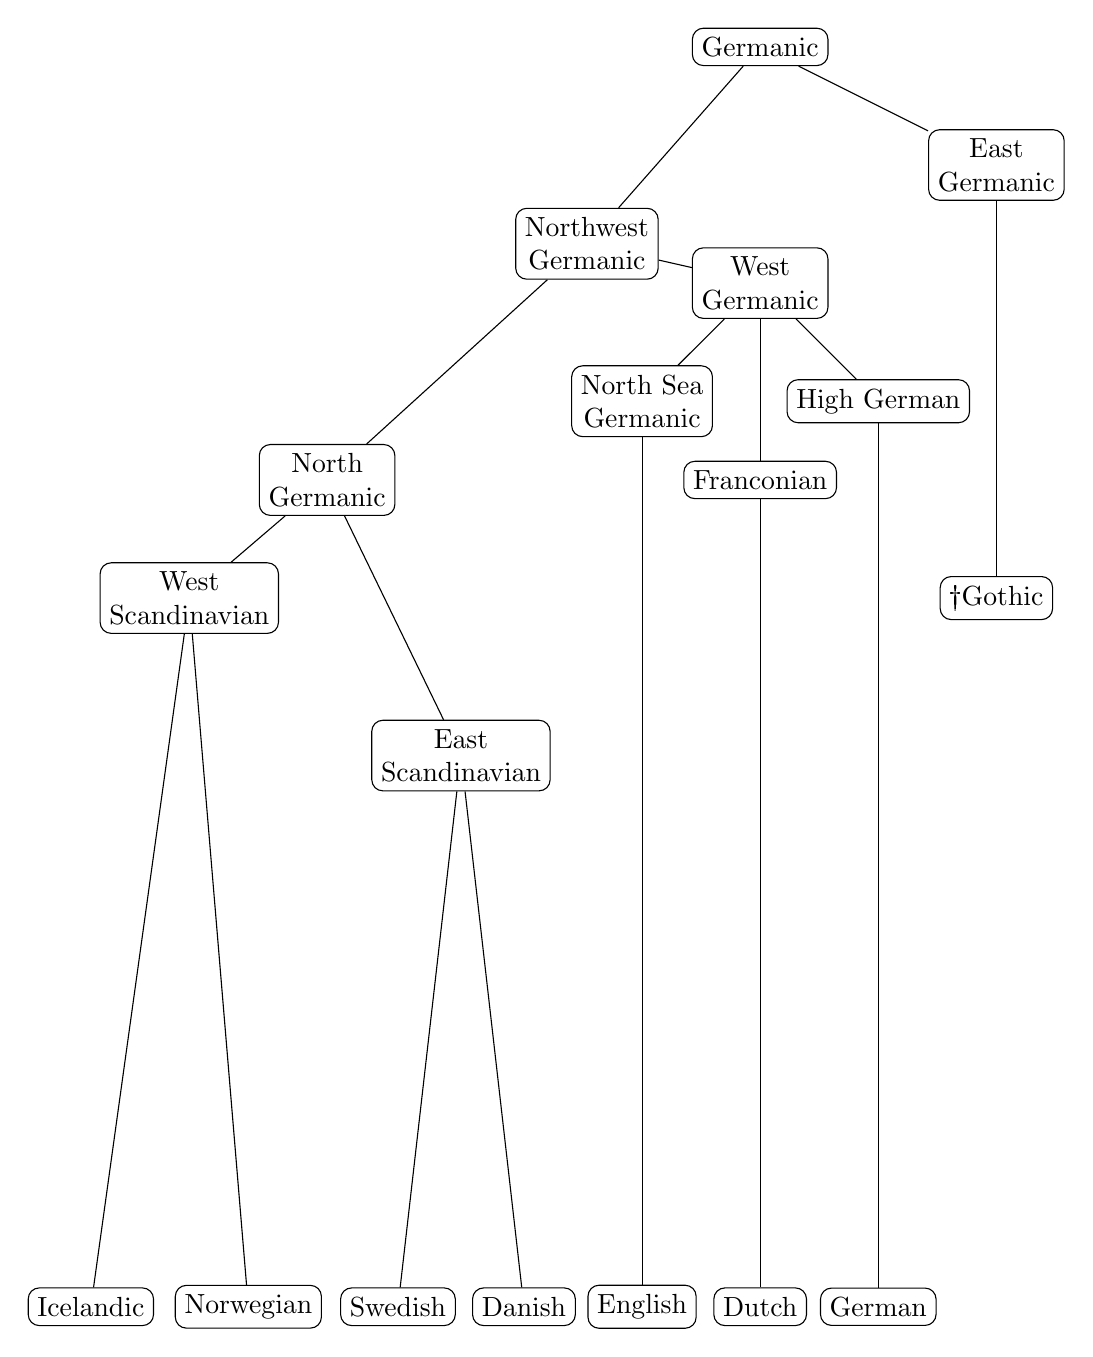
\begin{tikzpicture}[
  every node/.style = {shape=rectangle, rounded corners,
    draw, align=center,
    top color=white, bottom color=white}]]
  \node (G) at (8,16) {Germanic};
  \node (NWG) at (5.8,13.5)  {Northwest\\ Germanic};
  \node (NG) at (2.5,10.5) {North\\ Germanic};
  \node (WSc) at (0.75,9) {West\\ Scandinavian}; 
  \node (isl) at (-0.5,0) {Icelandic};
  \node (nor) at (1.5,0) {Norwegian};
  \node (ESc) at (4.2,7) {East\\ Scandinavian}; 
  \node (swe) at (3.4,0) {Swedish};
  \node (dan) at (5,0) {Danish};
  \node (WG) at (8,13) {West\\ Germanic};
  \node (NSG) at (6.5,11.5) {North Sea\\ Germanic};
  \node (eng) at (6.5,0) {English};
  \node (Frc) at (8,10.5) {Franconian}; 
  \node (nld) at (8,0) {Dutch};
  \node (HG) at (9.5,11.5) {High German}; 
  \node (deu) at (9.5,0) {German};
  \node (EG) at (11,14.5) {East\\ Germanic};
  \node (got) at (11,9) {\dag Gothic};
  
  \draw (G) -> (NWG);
  \draw (NWG) -> (NG);
  \draw (NG) -> (WSc);
  \draw (WSc) -> (isl);
  \draw (WSc) -> (nor);
  \draw (NG) -> (ESc);
  \draw (ESc) -> (swe);
  \draw (ESc) -> (dan);
  \draw (NWG) -> (WG);
  \draw (WG) -> (NSG);
  \draw (NSG) -> (eng);  
  \draw (WG) -> (Frc);
  \draw (Frc) -> (nld);
  \draw (WG) -> (HG);
  \draw (HG) -> (deu); 
  \draw (G) -> (EG);
  \draw (EG) -> (got);
  
\end{tikzpicture}
}
 \caption{A (partial) phylogenetic tree of Germanic languages}
 \label{germanic-tree}
\end{figure}

Languages which are descendants of the same proto-language are said to belong to the same \textit{\isi{language family}}. In practice, which languages are grouped together actually depends on whether the relationship between them has been proven. A family is thus not different in nature from any of its subgroups defined by a common proto-language, but whether we call it a family depends on the current state of our knowledge. The current partition of the world's languages into about 400 families (about half of these with only a single member) has however turned out to be remarkably stable for decades, indicating that the field might find itself near to a maximum time depth where enough similarites survive to prove genetic relationship. This maximum time depth is commonly assumed to lie between 6,000 and 8,000 years ago, with older relationships provable in the presence of old written records (as in the case of Afro-Asiatic\il{Afro-Asiatic languages}, a family with a time depth of about 10,000 years which 
includes ancient languages such as \ili{Hebrew}, \ili{Akkadian}, and \ili{Ancient Egyptian}).

Within the Indo-European language\il{Indo-European languages} family, the \ili{Germanic languages} form a \textit{\isi{taxon}}, i.e. a group of more closely related languages which in turn have a common ancestor. Often, families can be decomposed rather cleanly into several such taxa, whereas the question which taxon split off first is often difficult to answer and forms a large part of the debate among experts in the respective language family. The established taxa frequently correspond to a time depth of around 2,000 years, when the similarities between descendant languages are usually still so pervasive that the relationship is obvious to a layman taking a first glance at the basic vocabulary. For instance, it is quite obvious that \ili{English} \textit{wife}, \ili{German} \textit{Weib}, \ili{Dutch} \textit{wijf}, \ili{Swedish} \textit{viv}, and \ili{Icelandic} \textit{víf} are essentially the same word, and a dozen of these close parallels in basic vocabulary would be enough to define Germanic as a taxon.
 In contrast, proving that \ili{Armenian} \textit{kin}, \ili{Russian} \textit{žena}, \ili{Irish} \textit{bean}, \ili{Icelandic} \textit{kona}, and \ili{Persian} \textit{zan} are related in very much the same way, requires a lot more effort and expert knowledge, which is similar to the situation in many other families.

\section{Language contact and lateral connections}\label{sec:2:2}
What complicates the picture of neat family trees depicting in which order the languages of a family split off, is that languages are in contact\is{language contact} with each other, and that linguistic features do not only result from inheritance or random change, but also from \isi{borrowing} between languages which are in contact. To the non-linguist reader, the term \textit{borrowing} might seem slightly odd because the element taken from the donor language is never given back in any sense, in which case it helps to mentally equate borrowing with the copying of material. On the lexical level, a loan or \isi{loanword} is a word which gets copied by one language (the \isi{recipient language}) from another (the \isi{donor language}).

\ili{English} is a very good language for finding examples of contacts, as it represents a very interesting mix of inherited (Germanic) and borrowed (mostly Romance) features. On the level of morphology, English features two competing strategies of forming the comparative degree of an adjective, the Germanic suffix \textit{-er} as in \textit{larger} or \textit{thicker}, and the Romance-style pattern with \textit{more} as in \textit{more interesting} or \textit{more relevant}. The English lexicon is split roughly in half \citep{finkenstaedt_wolff_1973}, where the first half is dominated by basic vocabulary and words for everyday items and phenomena, which are typically either inherited from Proto-Germanic (\textit{eye}, \textit{rain}, \textit{hammer}) or borrowed from other \ili{Germanic languages} (\textit{window}, \textit{wing}, \textit{skin}). The other half mainly consists of terms of science and culture (\textit{science}, \textit{pious}, \textit{ignition}), all of which were borrowed from \ili{Latin} and 
\ili{Romance languages}. The convention is to consider the descent of the basic vocabulary and grammatical features as the relation defining the tree (and thereby the family membership), and to treat contact of any intensity as a secondary phenomenon, which makes English a Germanic rather than a Romance language.

Still, the sometimes very visible effects of language contact have always caused an undercurrent of historical linguistics to reject the tree model. Given the ubiquity of language contact, the underlying assumption of the tree model that languages continue to evolve independently after each split, and treating continued contact as the exceptional case, might seem unnatural. People in this school of thought have tended to adhere to an alternative \isi{wave model}, which is based on the observation that linguistic innovation tends to spread from a center to the periphery. Sometimes, innovations will sweep across language boundaries in situations of language contact, which then leads to borrowing. A language split occurs when a series of waves does not sweep across an entire language community. \citet{francois2014} provides a good recent overview of the theory behind wave models, and argues why they are attractive for describing some patterns of innovation. While generally accepted as well-suited for explaining areal phenomena and dialect continua, the strong assumption of wave-model advocates that any apparently tree-like signal in language evolution arises out of a pattern of overlapping waves is not advocated by many historical linguists any longer. While this view was once very popular due to certain phenomena in the history of Indo-European, it has been weakened by the abundance of quite clearly tree-like patterns in language families since studied. From the perspective of inference, wave models are problematic as well. The problem is that they have little explanatory value in the individual case, since every observable situation can be explained by many more different sequences of waves than sequences of splitting events which generate trees.

\largerpage[-1]
\section{Describing linguistic history}\label{sec:2:3}
Historical investigations about any given language often amount to proposing etymologies\is{etymology} for words. An etymology is a description of a word's history, typically featuring either the information which word in a reconstructed proto-language it evolved from, from which other language it was borrowed, or how it was derived from lexical material which already existed in the language. For instance, the etymology of the \ili{English} word \textit{house} is given by \cite{kroonen2013} as inherited from a reconstructed Proto-Germanic word \textit{*hūsa-}, which in turn is of obscure origin, although it might derive from a Proto-Indo-European root \textit{*kuH-} `to cover', which would connect the word to e.g. \ili{Latin} \textit{cutis} `skin' and \ili{Lithuanian} \textit{kiautas} `shell, rind, skin'. The etymologies one can establish thus vary in time depth, and tracing a word's history further into the past is a frequent type of contribution which would in this case advance our knowledge of Germanic. 
Etymological dictionaries for a single modern language will often include much more information about additional senses and when they developed, as well as the first attestations of some idioms involving the headword. This type of information is not required for the word to have an etymology, and most etymological dictionaries do not include such information, often due to a lack of historical data.

In classical historical linguistics, words which are derived from the same word in a common proto-language are called \textit{cognates}\is{cognate}, whereas borrowed words and their descendants are not counted as belonging to the same \isi{cognacy class}.
While the clean separation of inherited words and loanwords is crucial to the classical method, computational methods have tended to put less emphasis on this distinction. This leads to a somewhat unfortunate difference in terminology between classical and computational historical linguistics, as the latter customarily subsumes both inheritance and borrowing under the cognacy relation. As an alternative term to cover this more liberal notion of cognacy, \textit{correlate} has some currency, but I opt not to use it here because of the otherwise confusing frequent occurrence of the concept of correlates in the statistical sense in the text. Instead, I will use \textit{\isi{true cognacy}} for the stricter classical sense whenever the distinction is relevant, and otherwise stick to the more liberal usage established in computational historical linguistics.

Expanding on the basic distinction of inherited items and loans in the lexicon of a language lexicon, descriptions of loanwords are usually more fine-grained. Very often, loanwords of roughly the same age from the same donor languages can be grouped into strata\is{stratum} or layers. For instance, there is a rather thin stratum of Celtic\il{Celtic languages} loans in \ili{English}, which includes words such as \textit{basket}, \textit{beak}, and \textit{nook}. This Celtic stratum can be further subdivided into an \ili{Ancient Brittonic} layer (to which the mentioned words belong), and later borrowings from languages such as \ili{Welsh} (\textit{bard}, \textit{crag}) and \ili{Irish} (\textit{galore}, \textit{slogan}). In effect, the lexicon of every language can be split into an inherited core vocabulary, and a number of loanword strata which came into the language at different times from different languages.

\section{Classical methods}\label{sec:2:4}
This section provides a concise introduction into the mindset and the methods of classical historical linguistics, the discipline to which we owe the bulk of our current knowledge about the history of the world's languages, and against the results of which computational methods are commonly evaluated. Historical linguistics is a much broader field than a short introduction to core principles would suggest, and the non-linguist reader is encouraged to explore the field in its breadth by means of a handbook, such as the excellent recent one by \citet{bowern_evans_2015}.

\subsection{The comparative method}
The primary tool of historical linguistics is the \textit{\isi{comparative method}}, a well-tested set of principles which has been developing for about two centuries, and has proven its worth as a tool for reconstructing the history of many language families. The key idea is to build on the assumed (and rather robustly attested) regularity of sound changes to reduce the likelihood that observed similarities between words from different languages are only due to chance. For a group of languages, relationship is then proven by reconstructing the sound inventory and the phonetic shape of many words in an assumed common proto-language, and then explaining how the known forms in each descendant language evolved from their equivalent in the proto-language by a series of regular sound changes.



\subsubsection{Sound correspondences}
On the synchronic level, both inheritance and regular sound changes lead to recurring sound correspondences in cognate words. For instance, there is a fairly regular sound correspondence between word-initial \ili{English} \textit{p} {[pʰ]} and \ili{German} \textit{pf} [p⁀f], as evidenced by pairs like \textit{pan/Pfanne}, \textit{plum/Pflaume}, and \textit{pluck/pflücken}. The last two examples show that we cannot expect one-to-one correspondences across all comparable segments in cognate pairs: English \textit{u} [ø] can apparently correspond to German \textit{au} [ɑʊ̯​}]\todo{not plain [a]/} or \textit{ü} [ʏ].\todo{not [y]?} The reason for such a one-to-many correspondence can be either that two different phonemes have merged into English [ø], or that one proto-phoneme diverged into the two German variants due to a conditional sound law, i.e.\ a change which happened regularly in a specific phonological context, which might have left no traces in the observable forms.

\subsubsection{Sound laws}
In the Neogrammarian view, the sound correspondences between related languages are the result of \textit{sound laws}\is{sound law}, i.e.\ regular phonetic changes which occurred while the languages developed from their common proto-language. In the simplest case, a sound change replaces all occurrences of some sound by a different one. However, in reality, sound laws almost never occur unconditionally, i.e.\ they will typically only apply in a certain phonetic context (such as between vowels, or in stressed syllables). Due to this context dependency, sound changes can increase the number of phonemes in a language, whereas unconditional rules could only keep the number of phonemes constant (if the resulting phoneme was not present in the language before), or decrease it (if two phonemes merge). For instance, the phoneme [t⁀ʃ]\todo{if this is a phoneme, it should be //, not []} that is written \textit{ch} in modern \ili{English}, did not exist in West Germanic, and only developed during the Anglo-Frisian stage in a rather common process called 
palatalization, where velar plosives become palatals (often affricates) under the influence of adjacent front vowels. In other contexts, ancestral [k] was left untouched. This explains the seemingly irregular sound correspondence between English \textit{choose} (\ili{Old English} \textit{ċēosan}) and \ili{Dutch} \textit{kiezen}, whereas we have [k] in both English \textit{cat} and its Dutch cognate \textit{kat}.

The crucial idea of the Neogrammarian school of linguists is that such sound laws apply without exception, i.e.\ they apply to all instances of a sound in a particular context throughout the words of a language. These contexts can be quite complex, as can quickly be demonstrated using \ili{English} and \ili{German}. The sound law which produced the mentioned \textit{p/pf} correspondence between English and German is part of the second phase of the High German consonant shift. By comparing the contexts in which this correspondence as well as analogous instances of affricatization ([t] $\rightarrow$ [t⁀s] and [k] $\rightarrow$ [k⁀x]) occur, one finds that the law must have applied in four distinct contexts: word-initially, when geminated ([pː],[tː],[kː]), after liquids ([l] and [r]), and after nasals ([m] and [n]). For the \textit{p/pf} pair, we have already seen examples of the first context. Instances of the second context are \textit{apple/Apfel} and \textit{copper/Kupfer}. The liquid context is exemplified by \textit{carp/Karpfen}, and as examples of the nasal context we have \textit{swamp/Sumpf} and \textit{cramp/Krampf}. This pattern reliably repeats itself across all the lexical material which both languages inherited from West Germanic.

Since sound changes are historical events which happen during a short timeframe, the laws which shaped the history of a language can be arranged into a sequence in which they occurred. Because sound laws frequently interact (e.g.\ if one change creates a context where the next law can apply), we can often derive constraints on the possible order in which they must have occurred, leading at least to a partial relative chronology. For instance, we know that the third stage of the High German consonant shift, which in some \ili{German} dialects turned voiced plosives into voiceless ones (e.g.\ \textit{[b]} $\rightarrow$ \textit{[p]}, must have occurred after affricatization, because the voiceless stops would otherwise have become affricatized in turn. We can exlude this order of events based on the fact that the German cognate of English \textit{bread} is not \textit{*Pfrot}, but \textit{Brot}, which is pronounced something like [pʀoːt]\todo{maybe better [b̥]} in the dialects which underwent the third stage of the shift.

While we frequently can derive constraints on the relative order of sound changes in this way, an absolute chronology of sound changes is much more difficult to derive. Typically, it is necessary to rely on historical knowledge or written sources for this. For instance, we know for certain that the High German sound shift must have happened before the 8th century, because \ili{Old High German} texts from that time already display the results of that change. For written languages where we have no written sources in scripts which reveal the phonology, a (partial) relative chronology is often the best we can arrive at.

\subsubsection{Distinguishing inherited words from loans}
The work of establishing sound changes and their chronology is necessarily based on reflexes of the same proto-words across descendant languages. The groundwork of historical linguistics has therefore always revolved around the tasks of finding true cognates, distinguishing them from loans, and separating the loanwords in each language neatly into strata. This sometimes very complicated task forms the necessary preparatory work for later higher-level steps such as determining isoglosses, and reconstructing proto-languages in order to establish phylogenetic units.

In addition to reducing the likelihood of words becoming similar due to chance, the regularity of sound change also provides us with the most important source of hints about the etymology of words, especially when deciding whether some word was inherited, or borrowed from a sister language. For instance, the Proto-Germanic shift from [k] to [h] is enough to prove that \ili{Latin} \textit{cellarium} `pantry' and \ili{German} \textit{Keller} `cellar' cannot be true cognates, because we would expect something like \textit{*Heller} in this case. Although interactions between sound laws, and gaps in our knowledge about them, can make this type of argument quite complex, it is typically possible to recognize non-cognates, and estimate the time at which they were borrowed, for a large portion of a language's basic lexicon.

\subsubsection{Reconstructing ancestral forms}
With cognate sets and sound laws established, in theory it should become an almost mechanical task to project the attested words back to reconstructed proto-forms by reverse application of the sound laws. If this back-projection does not lead to the same proto-form if we start from different descendant languages, this is a hint that some of our current hypotheses about sound laws and cognacy relations must be wrong, and provides us with clues about the ways in which our theory needs to be revised.

In practice, there are many phenomena which complicate the picture, and make reconstruction of ancestral forms a non-trivial task. The most pervasive of these is \textit{analogy}, which subsumes a variety of very frequently occurring phenomena by which irregular changes can happen whenever the result becomes in some way easier to represent and process than the initial form. To quote two of the many examples given by \cite{campbell1999} in his introduction to historical linguistics, the vowel contrast between the \ili{English} adjective \textit{old} and its old comparative form \textit{elder} (which still survives in \textit{elder brother}) became leveled to yield current \textit{older}, and \ili{German} \textit{Natter} is cognate with English \texttt{adder}, which lost its initial \textit{n} due to reanalysis of its combination with the indefinite article, such that \textit{a nadder} became \textit{an adder}.

To give another more complex example from a different language family, the Proto-Uralic\il{Uralic languages} words \textit{*ükte} and \textit{*kakta} are one possible reconstruction for the numbers `one' and `two'. The latter should have resulted in \ili{Finnish} \textit{*kahda-} by regular sound change, but the actual form is \textit{kahde-}. In contrast, Finnish \textit{yhde-} `one' is the completely regular result of applying known sound laws to \textit{*ükte}. It is generally assumed that the irregular form \textit{kahde-} received its final vowel by analogy, making the words for the two numbers more similar. The decision that \textit{*kakta} and not \textit{*ükte} is the word that was reshaped is necessarily based on reflexes in other branches of Uralic, which demonstrates why analogy complicates reconstruction. In fact, because irregular changes also appear to have happened to \textit{*kakta} in other branches of Uralic, there is still no consensus whether \textit{*kakta} is actually the correct 
reconstruction.

Explanations involving analogy are very common in etymological research, and it seems that analogy is a force just as important as regular sound change in shaping words. For historical linguistics, relying too much on analogy when explaining word forms is quite risky, because allowing almost arbitrary sporadic changes to apply to only one or a few words makes it much easier to fit forms to any reconstructions, detracting from the strength of the method.

\subsubsection{Establishing phylogenies}
By reconstructing ancestral proto-forms for a set of cognates in a set of attested languages, and proving that the regular sound changes and additional assumptions such as analogies correctly generate the different attested forms from the reconstructed form, a historical linguist proves that the attested languages form a phylogenetic unit. By reconstructing older proto-languages as common ancestors of already established younger ones, it should in principle be possible to establish the entire phylogenetic tree of a language family, detailing in which order various genera split off the common proto-language, and how these in turn split into the attested languages.

If we continue this reconstruction process through the ages, shouldn't it be possible to trace the history of each language back to very few large families? If one assumes \textit{monogenesis}, i.e.\ that human language has only developed once, and not independently in different places, one could even imagine deriving a world tree, detailing how the modern human languages developed out of a single ancestral language of humankind.

Unsurprisingly, there are limits to the comparative method preventing us from getting this far. The more sound changes accumulate through the ages (especially under complicated conditions), the more indistinguishable the inherited similarities will be from chance similarities. To still isolate individual sound laws and unravel in which contexts and in which order they applied, we would need ever larger numbers of cognacy candidates. The most serious limitation for the method therefore lies in the fact that cognate density actually decreases. Due to semantic change, lexical replacement, and borrowing, the cognates shared between two related languages are bound to get lost with time. Since every language has only a finite number of basic lexemes, already after a few millennia the languages will cease to share enough cognates for regular sound correspondences to be established, and the comparative method ceases to work.

For well-documented language families, the limits of the comparative method in terms of establishing deep ancestry appear to have been reached quite some time ago. What is more, many families which are generally considered established (such as Afroasiatic, and Sino-Tibetan) are not proven as genetic units in the strict sense, as there are no single widely accepted reconstructions of the respective proto-languages. The maximum age of phylogenetic units which can still be safely established using the comparative method seems to lie at between 6,000 and 8,000 years before present, which leads us far into prehistory in most parts of the world, but is a far cry from being able to get back to the times when e.g.\ the Americas or Australia were settled. Any method which tries to answer questions at higher time depths based on language data will need to resort to statistical arguments, or typological similarities, both of which cannot rule out the possibilities of chance similarity (a risk which is high for 
typological variables due to universals) and ancient contact.

\subsubsection{Shared retentions and innovations}
But the methodological limits of the comparative method do not only appear at high time depths, but also when making family-internal classification decisions. To reliably separate one taxon from the rest of the family, the amount of lexical overlap in terms of shared cognates is considered an insufficient criterion. Even if we excluded the possibility of borrowing, a larger-than-average lexical overlap between two languages we want to group together can still be either due to shared retentions (the languages outside the group under consideration changed) or shared innovations (the change happened from the proto-language of the family to the taxon we are trying to establish). The existence of correspondences alone does not yet allow us to decide whether we are dealing with shared retentions or innovations. The main reason why many subgroupings which seem obvious on a lexical level are sometimes not generally accepted is that quite often, the hypothetical common proto-language is so close to the proto-language 
of the entire family that no regular changes can be detected to define the transition between the two proto-languages. The requirement of demonstrable shared innovations often severely limits the ability of classical historical linguists to clarify the internal structure of a language family beyond the level of securely established branches.

\subsection{Theories of lexical contact}
Whenever speakers of two different languages get in intensive contact with each other, this will invariably leave traces in those languages. According to \citet[Section 8.5]{hock_joseph_1996}, the main variable deciding about the shape of lexical influence between two languages is the difference in prestige. This difference is the standard explanation for the fact that languages do not only borrow needed words for new concepts (such as \ili{German} \textit{Computer} and \textit{Internet}), but also tend to replace perfectly workable and well-established terms for some concepts with those from a prestige language (German \textit{Service} instead of \textit{Dienstleistung}, or \textit{Ticket} instead of \textit{Fahrkarte}).

As \citet{thomason_kaufman_1988} elaborate in their analysis of contact situations, the decisive factor determining how a contact situation between a high-prestige and a low-prestige language plays out is whether it occurs under conditions of maintaining the low-prestige language, or language shift towards the high-prestige language. The first scenario will typically lead to a situation of widespread bilingualism, where even words for basic concepts tend to be replaced by their borrowed equivalents, as the familarity of the bilinguals with the higher-prestige language increases at the expense of the lower-prestige recipient language. The situation where the prestige gradient is not too high, and both languages continue to coexist for many generations, is the one where one would expect the largest amount of borrowings even of basic vocabulary items. The words borrowed from a language of comparable prestige are said to form an adstratum. For instance, \ili{English} has a North Germanic\il{North Germanic languages} 
adstratum from the time when the Vikings settled large parts of England, and started to intermarry with the local population. Words borrowed by English during this time include very basic vocabulary items such as \textit{to take} and \textit{they}.

In the second scenario, the target language is learned imperfectly by shifting speakers, which tend to retain many phonological and syntactic features of the original language, but typically not much lexical material except terms for local plants and animals. If the number of shifting speakers is demographically relevant, the structural \isi{substrate} influence will result in a changed variant of the target language. A case in point is the Western Uralic substrate in \ili{Russian} which shows itself in certain syntactic features which set Russian apart from its Slavic sister languages, such as the lack of a copula in the present tense, and the extensive use of the partitive genitive.

In the case where both languages are maintained (i.e.\ in the absence of language shift), \citet{thomason_kaufman_1988} distinguish five degrees of contact intensity, each with characteristic manifestations in the extent of lexical and structural borrowing. The first three stages represent different degrees of lexical borrowing, with accompanying weak structural borrowing that does not cause any shifts in the typological profile. Under circumstances of casual contact, we would only expect content words to be borrowed, and typically non-basic vocabulary. Under slightly more intense contact, conjunctions and adverbial particles will be among the first structural elements which are taken over. Only under very intense contact will we observe borrowing of other function words such as adpositions, pronouns, and low numerals. Bound morphemes such as derivational affixes may also be transferred at this stage, and they can stay functional in the borrowing language. The last two stages describe situations of strong 
and very strong cultural pressure, where the structural influence is so strong that typological changes can occur. On the lexical level, contact of this intensity will lead to massive borrowing which can even replace large parts of the basic vocabulary.

\subsubsection{Types of borrowing}
In the bilingual environment where most lexical borrowings occur, a loanword is initially borrowed in its original phonetic shape. With time, loans tend to get nativized by sound changes, often up to a point where they are not recognizably foreign any longer. An instance of this is \ili{German} \textit{Fenster} `window', which was borrowed from \ili{Latin} \textit{fenestra} into \ili{Old High German}, i.e.\ more than a thousand years ago. Without knowledge of Latin, no native speaker of German would suspect that this word was not inherited from the parent language. By contrast, more recent loans in German, such as \textit{E-Mail} from \ili{English}, tend to contain sounds foreign to German (the diphthong [eɪ]), or to deviate from the usual orthographic rules (the long vowel [iː] written as \textit{e}, instead of \textit{ie} or \textit{ih}), and are therefore instantly recognized as loanwords.

While from the perspective of cognacy, borrowing across families will tend to be detectable as words from a different cognate class, the quite common situation of \isi{internal borrowing} within the same language family often leads to a word getting replaced by a cognate word from a sister language. For instance, this is what happened with the \ili{English} word \textit{guard}, which replaced older \textit{ward} by a cognate borrowed from \ili{Frankish} via \ili{French}, where a regular sound change from [w] to [ɡ] had occurred (cf. \textit{William} vs. \textit{Guillaume}). Both cross-family and family-internal borrowing will commonly happen whenever living languages come into close contact.

A lot less frequently, words can also be borrowed from ancient languages, which might even be direct ancestors of the recipient language. This tends to happen with high-prestige written languages that persist as languages of religion or science. The most well-known examples are Latin in Western and Southern Europe, from which \ili{Romance languages} did not only inherit, but also borrow words, and \ili{Sanskrit}, which plays the same role across India. Less well-known examples of the same pattern include \ili{Old Church Slavonic}, from which many words were borrowed into later East Slavic languages such as Russian, and the influence of \ili{Pali}, the Middle Indo-Aryan language of Theravada Buddhism, on many languages of Southeast Asia. If a language borrows from its own ancestor or a close relative, this very frequently leads to doublets like the \textit{guard/ward} example, which are also called etymological twins. For instance, the Latin word \textit{dīrectus} developed into French \textit{droit} under regular sound change, but the word \textit{direct} was later borrowed into French in addition, where the two words now coexist.

In addition to loanwords, \textit{calques} are the second important type of lexical borrowing. A calque, also called loan translation, is a derived word which is composed of native lexical material after the model of a derived word in another language. For instance, the \ili{Hungarian} \textit{összefüggés} `correlation' is composed of the native lexemes \textit{össze} `together' and \textit{függ} `to hang' after the model of \ili{German} \textit{Zusammenhang} `correlation', literally `hanging-together'. Massive calquing tends to occur when the vocabulary of a language needs to be expanded rapidly to areas of life that it was not previously applied to (e.g.\ science or technology), and is especially pervasive when compounding is a preferred word formation strategy in both the model language and the newly expanded one, as has been the case for German and Hungarian. The term `borrowing' as used in this book does not include calques.

\subsubsection{Constraints on borrowing}
As \citet{haspelmath2008} states in his summary of loanword typology, an essential step towards a theory of language contact is to determine possible constraints governing which elements of a language are more likely to be borrowed, and in which order elements will be borrowed under intensive contact. From the viewpoint of historical linguistics, understanding these constraints can help to decide open questions in language classification. In the context of the present volume, this knowledge will be of some use in interpreting results, and feeds into the design of a simulation model of some aspects of actually occurring lexical transfer.

The most striking initial observation about borrowability is that the number of content words which can be transferred during intensive contacts seems almost unconstrained. Less than half of the vocabulary of modern \ili{English} is of Germanic descent, and \ili{Armenian} has borrowed so many words from neighboring \ili{Iranian languages} that its nature as a separate branch of Indo-European was only recognized very late in the history of Indo-European linguistics. However, we have already seen that words for the most basic vocabulary are typically exchanged only among languages of roughly equal prestige in long-term contact. This kind of contact is historically quite rare at least in the regions of the world that I will be concerned with here, meaning that basic vocabulary will be a very good predictor of genetic affiliation.

Beyond such general statements about basic and non-basic vocabulary, scholars have established some non-trivial constraints on the borrowability of different parts of the lexicon which seem worth mentioning. For instance, an important factor to which much influence has been attributed is the typological distance between the donor and recipient languages, because very different grammars make it harder to copy words, let alone grammatical features, without causing major changes to the recipient language's system. This helps to explain why conjunctions and adverbial particles are borrowed more often than other functional items. These elements belong to smaller subsystems which tend to be less integrated with the rest of the grammatical system, and are thus more likely to be integrable into the structural fabric of the borrowing language.

Calling into question the predictive power of such theories, \citet{thomason_kaufman_1988} attack the central role attributed to structural incompatibility as an explanation of resistance to lexical borrowing. Based on some very interesting extreme cases, they argue that any prediction about which parts of the lexicon and the grammatical structure are susceptible to borrowing will mainly need to build on sociolinguistic factors. Under social circumstances which are conducive to moderate borrowing, however, typological compatibility still appears to influence the extent of structural borrowing, sometimes leading to more intensive interference than one would expect at the given intensity of contact.

Beyond compatibility, an important inhibiting factor for the borrowability of a feature appears to be its overall typological markedness. For instance, morphemes which express more than one function (such as the combined case and number markers of Indo-European languages) are less likely to be borrowed than the typologically more common clearly separable and single-function morphemes (such as case endings of agglutinating languages). Beyond such individual cases, if we consider morphological means to express functions as generally more marked than syntactic means, this general principle can also explain the tendency for morphological complexity to reduce in contact situations.

On the lexical layer, there are differences in borrowability between different types of content words. Most prominently, nouns are borrowed more easily than verbs. This long-held view was substantiated by \citet{van-hout_muysken_1994}, who statistically analysed texts for different factors which predict the borrowability of lexical items from \ili{Spanish} into Quechua. Their explanation for finding many more borrowed nouns than verbs is the motivation of extending referential potential, i.e.\ giving words to new things. Since new things which need a name are much more common than new actions, this explains the higher borrowability of nouns. But they also find a signal in favor of borrowing lexemes which show little inflection in the donor language. The latter finding ties in well with the theory of language contact developed by \citet[Ch. 6]{myers-scotton2002}, who argues that the main reason for the higher borrowability of nouns as opposed to verbs is that introducing foreign noun phrases tends to be less 
disruptive to predicate-argument structure.

A well-known phenomenon that can be interpreted as reinforcing this theory was first observed by \citet{moravcsik1975}, who claimed that words for verbal concepts are never borrowed as verbs, and only become borrowable as nominalizations. The part of this extreme claim which still remains valid today in the presence of much more evidence is that languages with complex verbal morphology do not tend to borrow verb stems from other languages, nor act as donors of verbal stems. Instead, verbal concepts are much more likely to be borrowed in the shape of nouns, typically in the form of a source-language nominalization which is then combined with a light verb meaning `to do'. For instance, this pattern appears very strongly in the \ili{Arabic} influence on the languages of many Islamic cultures. The Semitic root-pattern morphology is so alien to languages from other families, that they will only borrow verbs in a nominalized form. For instance, the Arabic verb \textit{daʿ\={a}ʾ} `to summon' was borrowed as a 
verbal noun (\textit{duʿ\={a}ʾ}) into languages from other families, where it was combined with native light verbs to express the concept of praying. In \ili{Persian}, this gives us \textit{do'\^{a} kardan} `to pray', whereas the \ili{Turkish} and \ili{Uzbek} equivalents are \textit{dua etmek} and \textit{duo qilmoq}, respectively. This strategy of integrating Arabic loans is extremely common in all major Iranian and Turkic languages. Instances of the same strategy are observed many times across the globe by \citet{wichmann_wohlgemuth_2008}, who place it at the lower end of a tentative loan verb integration hierarchy. The partial cognacy relations which result from this type of borrowing become a problem for any attempt to automatically partition the words for a given concept across many languages into cognate classes.

\subsubsection{Mixed languages}
Some languages have interacted with other languages to such a degree that their genetic affiliation becomes difficult to define. The most common type of such mixed languages are the \textit{creoles}\is{creole}, fully developed languages which come into being when a \textit{pidgin}, a simplified auxiliary language as it tends to arise when speakers of very different languages need to communicate, gets nativized by children growing up with the pidgin as their primary language.

The prototypical creole languages all arose from colonization, where the colonial language invariably operates as the \textit{lexifier} of the creole language, i.e.\ virtually the entire lexicon is inherited from the colonial language, albeit undergoing sometimes significant semantic change. The substrate influence of the other language is seen in the grammatical structure (which often retains little similarity with the lexifier), and often in collocations and idioms. For instance, \ili{Tok Pisin}, the national language of Papua New Guinea, is an English-based creole where the word \textit{gras} `grass' has taken on the primary meaning `hair', via the indigenous conceptualization of hair as \textit{gras bilong het} `grass belonging to the head'. But apart from the prototypical colonial situation, other languages are sometimes discussed as possibly being creoles as well, especially when massive shifts within the grammatical systems can be shown to have occurred within few generations. The most famous example 
of this is \ili{English} itself, which was heavily restructured during the \ili{Middle English} period, losing almost all inflected forms and becoming extremely simplified in the remaining inflections such as plural formation. What makes this case less prototypical is that the two involved languages were related (making structural borrowing much easier), and that there was no clear developmental gap between the two cultures which would have ensured dominance. This also explains why in this case, the lower-prestige language would have to be treated as the lexifier.

While mixed languages can be difficult to classify in terms of phylogeny if our desire is to trace the development of the entire language system, on the description level of the lexicon, which the work described here is confining itself to, it is entirely unproblematic to just model creoles as immediate descendants of their lexifiers. Therefore, we do not need to be too concerned here with languages that might not have a clear position in a phylogenetic tree, and we can always assume an underlying tree-shaped skeleton to exist in our networks. On the lexical level, one could summarize the position I am taking as follows: there are no equal mixtures of languages, there are only admixtures. In biological terms, we have no hybridization, but potentially massive horizontal gene transfer.

\section{Automated methods}\label{sec:2:5}
Looking up many words in dictionaries, cross-referencing them and constantly re-performing these steps when revising earlier findings while solving the puzzle of a language family's development, can be a very time-consuming and even tedious task. Not surprisingly, the potential advantages of being able to automate subtasks in historical linguistics were seen as soon as computing technology became performant enough to operate on large quantities of string data. 

The earliest example of applying computers to a problem of historical linguists I was able to find is \citet{hewson1974}, who uses predefined correspondences between \ili{Algonquian languages} and simple sequences of substitutions to generate all possible projections from attested words into possible Proto-Algonquian forms, and filters out all candidate forms which are reconstructable by some sequence of substitutions from each modern form to arrive at a consistent reconstruction hypothesis. According to the author, this procedure resulted in the detection of 250 previously unknown cognate sets, and was then used as a core for a computer-generated etymological dictionary. From the description it is clear that the system exploits much previous knowledge, both in the representation and preprocessing of the input data, which will not be easily transferable to other language families.

One step closer to modern statistical methods, the COGNATE system first presented in \citet{guy1984} estimated the probability of sound correspondences using chi-square tests on a sound co-occurrence table based on string positions. The system was evaluated on 300-word lists from 75 languages of Vanuatu, and is reported to have yielded satisfactory results for closely related languages. Unfortunately, neither the system nor the test data appear to remain available.

\citet{embleton1986} summarizes early developments in lexicostatistics, but also foreshadows many of the approaches and concepts which still figure centrally in phylogenetic inference. For instance, Embleton proposes the use of clustering algorithms for deriving phylogenetic trees (including branch lengths) from cognate data, and uses a simulation model to analyze the amount of skew in tree inference introduced by borrowing. The discussion also addresses many of the major issues that the field is still struggling to solve, such as the lack of truly independent linguistic features, or the problems caused by selection bias in lists of shared roots or grammatical features that are extracted from the specialist literature.

A factor which hampered progress in this and many other computational fields was the lack of sufficient computing power for testing the already quite advanced algorithmic ideas of these pioneers of computational historical linguistics on substantial amounts of data. When it became clear that these limitations made the early tools too inflexible und unwieldy to attain general acceptance and widespread use among historical linguists, the field did not see any work for about a decade. It was only in the late 1990s that the successes of computational methods in biology inspired a second wave of attention for introducing automatization into other branches of science where the gene metaphor seemed fruitful. Among others, these included literary studies (tracing how works were derived from each other), anthropology (attempting to reconstruct ancient systems of kinship), and linguistics.

This section gives a rough overview of recent developments in applying computational methods to answering questions of relevance to historical linguistics. The discussion is restricted to methods which attempt to find answers to concrete questions about the past of words and languages, and does not include more general results which can be derived from large databases, such as computational proofs of claimed typological universals like sound symbolism, or global correlations involving extralinguistic features such as altitude, climate, and population size.

\subsection{Lexical databases}\label{sec:2.5.1}
The most basic prerequisite for any computational study in historical linguistics is an electronic database which contains the information a linguist would look up in dictionaries or other sources in a standardized format which can be processed by a computer. The absence of such databases has been one of the limiting factors in the expansion of the field, but some very useful resources have become available during the past decade, and the pace at which new resources appear seems to be accelerating.

While databases of typological features have only recently started to receive broad attention, most work so far has been performed on representations of the basic lexicon across a relevant set of languages. Such lexical databases either contain phonetic forms representing the realizations of a concept across the relevant languages in a unified format, or, especially when they cover data within well-known families, the realizations are cognacy-coded. The advantages and disadvantages of these types of databases, as well as examples of both types, are discussed in this section.

\subsubsection{Databases of phonetic forms}
The easiest way to generate some computationally tractable data about a set of languages is to take a list of basic concepts (the words for which still tend to be cognate among more distantly related languages), and dictionaries, and then digitalize the relevant entries, transcribing them from the orthography or the format used in the source into some cross-linguistically applicable string format, usually over some phonetic alphabet which allows to represent all the phonemes of the language family of interest. Many factors complicate this basic procedure, such as the need to bridge different gloss languages in different sources, the low availability of unpublished resources like fieldnotes, inadequate phonetic descriptions which make it impossible to reconstruct the pronunciation at the desired level of detail, grammatical properties which make expert knowledge necessary to isolate the relevant parts of dictionary forms, and imprecise glosses which leave the compiler without certainty that the intended 
concept was matched. Still, with some experience, very little is needed to compile a database of phonetic forms corresponding to a list of basic concepts. This is the main advantage of settling for phonetic forms, as opposed to more high-level data.

The earliest major effort to create a computer-readable database of basic vocabulary was part of the Automated Similarity Judgment Program (ASJP)\is{ASJP database}. The ASJP database aims to cover the words for 40 basic concepts across all documented languages, in a rather rough, but unified phonetic transcription. Version 18 \citep{asjp18}, the most recent version available at the time of writing, includes 7,655 wordlists. While some of these wordlists do not correspond to different languages, but variants of the same language, the number of languages still approaches about two thirds of the global estimate of currently spoken languages. Altogether, the database approaches a size of 310,000 entries, making it by far the largest currently available resource in one consistent format. Over the years, previous versions of ASJP have been used to investigate many linguistic questions like the stability of concepts against borrowing and semantic change, the question whether sound symbolism creates problematic 
amounts of lexical similarity between unrelated languages, and correlations between phoneme inventories and extralinguistic factors such as population size or geographic isolation.

More recently, \citet{greenhill2015} presented TransNewGuinea.org, a database covering more than 1,000 languages and dialects of New Guinea. The database represents a massive effort to make lexical data on the basic vocabulary of \ili{Papuan languages}, the least well-studied linguistic region of the world, readily available to a wider public on the web. Building on a list of 1027 lexical meanings, various types of published and unpublished resources were processed to build a database in a unified phonetic format that can be processed by computational tools. Due to the very sparse documentation of many languages, at the time of publication the total size of the database had only reached about 145,000 entries, or an average of just over 140 words per language. Work to expand the database by cognacy judgments is under way, but since the bulk of available material has already been processed, it will not be possible for this database to become much larger.

The Chirila database of \ili{Australian languages} by \citet{bowern2016} is another good example of a database spanning an entire linguistic region, with the goal to eventually make all known lexical data available. Due to the complicated legal situation when publishing full resources, and a cultural bias of many linguistic groups against giving outsiders access to their languages, only 230,000 of about a million database entries are freely available at the moment, but even this lower number puts Chirila among the largest available databases. In addition to documenting the word forms in the original sources, much effort is put into clarifying or reconstructing the most likely pronunciation in order to arrive at standardized phonemic representations.

The NorthEuraLex (North Eurasian Lexicon)\is{NorthEuraLex} database first presented in \citet{dellert2015a} is similar to the previous two databases in its aim to cover an entire linguistic area, but has the advantage of containing only very few gaps despite covering 1,016 concepts, which is only possible due to the much better documentation of minority languages in Europe and Russia. The version of NorthEuraLex which I will be using for evaluation covers 107 languages, making it comparable in size to the released parts of the Papuan and Australian databases. Since the compilation of NorthEuraLex was a substantial part of the necessary preparatory work for my experiments, as it provides the gold standard for evaluating my lexical flow methods, it will be discussed in much more detail in \chapref{sec:4}.

The examples of databases just listed are only the tip of an iceberg of smaller often unpublished databases which cover a single language family or the minority languages of one country. As can be seen from the recent dates of most publications, there has been an explosion in the number of large-scale lexical database projects during the last two years, a trend which can be expected to gain traction as the field continues to grow.

\subsubsection{Cognate databases}
The other type of lexical database does not consider the phonetic forms of primary importance, but encodes the presence or absence of cognate classes in each individual language. A phonetic database would focus on the information that the words for \textit{hand} in \ili{Armenian}, \ili{Albanian}, \ili{Greek}, and \ili{Georgian} are 
{[[d⁀z]εrkʰ]}, 
{[dɔɾə]},
{[çeɾi]}, and
\ipa{[χεlɪ]}, 
allowing a program to compare these strings in order to figure out whether they are related. In contrast, a cognate database would not provide the three words in a unified phonetic format, but instead encode the information that the first three words are cognates, while the fourth is unrelated, by assigning a \texttt{1} to the first three languages  and a \texttt{0} to Georgian in a column encoding the absence or presence of this cognate set.

The advantages of cognacy encoding are that binary characters are easier to handle computationally, and that many disturbing factors such as loanwords or morphology are already filtered out during data preparation, leading to much cleaner data. The disadvantage is that cognacy-encoded databases need to be compiled either by experts in the history of the respective language family, or by going through the published etymological literature in language families where such work exists. Both approaches require an enormous amount of work, which makes typical cognacy-annotated databases much smaller than phonetic form databases, and also limits the number of language families for which they are available.

A very early cognate database is the Dyen database which formed the basis of \citet{dyen_ea_1992}, an early lexicostatistical study of Indo-European. The database is a small and rather unreliable resource \citep{geisler_list_2010} which covers 200 concept across 84 \ili{Indo-European languages} in cognacy-encoded form. After substantial revisions, it today forms the core of \isi{IELex} \citep{ielex}, a database of increased quality which is continuously being updated, and will soon be released in a major revision. The most recent publicly available version groups about 35,000 words into 5,000 cognate sets.

An equivalent of IELex for the Uralic language\il{Uralic languages} family is collected under the name \isi{UraLex}. The latest available version of UraLex was published together with a phylogenetic analysis of the data by \citet{syrjanen_ea_2013}, when the database covered 226 concepts across 17 languages. Given the small size but high time depth of the language family, the very distributed state of etymological information, and considerable disagreement between different authors, even compilation of this small database has certainly been a substantial effort.

By far the largest effort so far is the Austronesian Basic Vocabulary Database (ABVD)\is{ABVD database} compiled by \citet{greenhill_ea_2008}, which covers 210 concepts across more than 1,400 languages, providing virtually complete coverage of the world's largest language family\il{Austronesian languages}. ABVD partially relies on orthographic forms instead of a fully unified transcription, otherwise it would provide another phonetic form database of a size comparable to the ASJP database, due to its deeper coverage of individual languages. What makes this database unique, however, is that words from a sample of 400 languages (an earlier version of the database) are grouped into more than 34,000 cognate sets. The low time depth of many genetic subunits tends to make these cognate sets a little less interesting than the long-distance cognates from the other databases, but the cognacy-annotated part of ABVD is poised to remain the largest database with expert cognacy annotations for quite some time.

\subsection{Phylogenetic inference}\label{sec:2.5.2}
A major focus of computational historical linguistics has been \isi{phylogenetic inference}, i.e.\ the task of inferring phylogenetic trees from language data. The bulk of work in phylogenetic inference has been character-based, typically building on cognacy data encoded in such a way that the presence of each cognate class is treated as a binary character. The older distance-based methods, where a single distance matrix between languages (which can be computed from string data in many different ways) is used to extract tree-like signals, have recently regained some popularity, especially for investigating language families where cognacy-encoded databases do not exist.

Phylogenetic inference already was a well-developed branch of bioinformatics when it started to be applied to large amounts of language data. Computing an optimal tree is inherently a very demanding problem because already the number of possible tree topologies over $k$ languages rises super-exponentially with $k$, and this does not yet include the inference of branch lengths. Exhaustive optimization according to some optimality criterion is therefore not an option. Instead, heuristic methods are employed, with the risk of hitting a local instead of the global optimum. The following summary is based on \citet{felsenstein2004}, a very popular book-length introduction to phylogenetic tree inference which is also recommended to the reader as an entry point to the field.

Phylogenetic inference methods can be classified as either distance-based or character-based. The distance-based case is the more general one, because any character-encoded dataset can be reduced to a distance matrix in a number of ways. However, the loss of information caused by reducing a character matrix into a simple language distance matrix will typically lead to lower-quality results, so that distance-based method will not typically be used if character-encoded data is available.

Assume we want to infer the best tree from a distance matrix. An ideal distance matrix would correspond directly to some tree by having the property that for any triple $A,B,C$ with structure $((A,B),C)$ [i.e $A$ and $B$ are closer, and $C$ more distantly related], the distance measure fulfills the conditions $d(A,B) < d(A,C)$ and $d(A,B) < d(B,C)$. However, a distance matrix which unambiguously encodes a single tree topology is rarely observed in practice. The reason can be noise introduced by errors in the underlying data, an inadequate distance measure, or a real non-tree-like signal resulting e.g.\ from loanwords in linguistics, or from horizontal gene transfer in biology. Multiple standard algorithms exist for quickly extracting a plausible tree from a distance matrix which does not consistently represent a tree. These approaches differ in complexity, and in the criterion they optimize.

The oldest and still frequently used distance matrix algorithm is \isi{UPGMA}, first defined by \citet{sokal_michener_1958} as an approach to hierarchical clustering. UPGMA (Unweighted Pair Group Method with Arithmetic Mean) progressively fuses clusters into larger phylogenetic units, starting with every node in its own cluster. The algorithm maintains a table of current distances between all clusters. At each step, the two clusters with the minimal distance are fused into a new cluster, and a corresponding node is introduced to the phylogeny. The distance between the new cluster and all existing clusters is defined as a weighted average of the distances to the two clusters, with the weights defined by their relative sizes. Branch lengths are simply defined by the distances among the clusters. UPGMA works quite well on data for which a clock assumption holds, i.e.\ when we can assume that the changes which increased the distance occurred at roughly equal rates throughout the tree. Under this condition, the 
UPGMA tree provides the optimal least-square fit between the branch lengths and the distance matrix.

If the length of tree branches is to be minimized wihout a clock assumption, the most popular quick approach is the \isi{neighbor-joining algorithm} by \citet{saitou_nei_1987}, which is not linked to a simple optimality criterion. Neighbor joining maintains a measure of isolatedness $u(i)$ for each node $i$, derived from its average distance to all other nodes. At each step, it connects the nodes $i$ and $j$ which have the smallest $d(i,j) - u(i) - u(j)$, i.e.\ distance corrected for isolatedness. The distance of the new node $ij$ to each existing node $k$ is then defined as $d(ij,k) := (d(i,k) + d(j,k) - d(i,j))/2$. i.e.\ the average of the distances to each of the two nodes, with a discount which increases as clusters become less closely connected. This procedure maintains a good balance between internal consistency of clusters, and quick inclusion of isolated nodes which are not particulary close to any other cluster.

If character-encoded data is available, the most straightforward optimality criterion is to build the tree which minimizes the number of assumed evolutionary events. This leads to the \textit{\isi{maximum parsimony}} paradigm, where the primary design decision is how to count the evolutionary events the number of which we want to minimize. The most straightforward definition is based on the minimal number of character-state changes we have to assume to fit the data to a given tree. Computing this number is typically done according to \citet{sankoff1975}, a dynamic programming algorithm which reconstructs the optimal character states at ancestral nodes as a byproduct. We will therefore take a look at the Sankoff algorithm in detail when reconstructing the presence of cognate sets at proto-languages in \sectref{sec:6.8}. Parsimony scores for any given tree can be computed very efficiently, but the challenge remains how to traverse the tree space in order to find a tree of maximum parsimony. The most advanced methods 
for doing that are based on the branch \& bound paradigm, where the entire search space is indexed by a decision tree. For each of the alternatives at the current decision node, lower and upper bounds for the still attainable parsimony scores are computed given the decisions already made. If the lower bound of one alternative is higher than the upper bound of the other, an entire (possibly huge) branch of the search tree can be ignored in our search for the maximum. With a good decision tree that maximizes the chances of large differences between alternatives, branch \& bound optimization can be quite efficient.

\citet{gray_jordan_2000} were the first to apply maximum-parsimony phylogenetic inference on substantial amounts of language data to answer an open question of historical linguistics. Using maximum-parsimony trees over 77 languages inferred from about 5,000 cognacy characters, Gray and Jordan compare two competing theories about the Austronesian\il{Austronesian languages} settlement of the Pacific. While the resulting trees clearly suggest a rapid expansion from Taiwan into Polynesia, they find that the overall signal does not fit the tree model extremely well, suggesting substantial interaction between populations even after the initial settlement. In contrast, \citet{holden2002} shows that the cognacy pattern for 92 concepts across 73 \ili{Bantu languages} fits a tree-like pattern rather well. The subgroupings with the highest support (i.e.\ which consistently appear across a range of maximum-parsimony trees on subsets of the data) were found to closely mirror the earliest farming traditions of sub-Saharan Africa, leading to the conclusion that the modern subgroups have largely remained in place since they became separated, without intensive contact or further large-scale migrations after the initial expansion.

The most modern and most successful approaches to phylogenetic inference are all \textit{probabilistic}, i.e.\ they build on a model specifying the probability of generating the character-encoded dataset from any hypothesized tree. This requires the generation of trees to be modeled explicitly by an evolutionary model, which can e.g.\ include separate mutation rates for each branch. However we define our evolutionary model, it will assign a probability $p(D|T)$ to the dataset $D$ given any tree hypothesis $T$. Now, if our goal is to find the tree $T$ which maximizes $p(D|T)$, we do not actually need to normalize $p(D|T)$ into a probability distribution by considering all other datasets, but it is enough to have some function which ranks trees in the same way as $p(D|T)$ on our fixed dataset $D$. A function $L(T|D)$ with this property is called a \textit{likelihood function}, and the resulting paradigm is therefore called \textit{\isi{maximum likelihood}}. As in the case of maximum parsimony, the challenge is 
to efficiently traverse the tree space in order to arrive at high likelihood values. Typically, the topology will be modified first, and the branch lengths then optimized given the topology. While naive optimization algorithms often work surprisingly well, a lot of technical machinery is needed to efficiently come up with good tree hypotheses on larger datasets. \citet[Ch. 16]{felsenstein2004} is still a good entry point into the ever-growing landscape of algorithms and heuristic techniques trying to solve this challenge.

Further exploiting the advantages of fully probabilistic models, the state of the art in phylogenetic inference relies on \isi{Bayesian methods}. If we have prior knowledge $p(T)$ about likely tree topologies, mutation rates and branch lengths (e.g.\ due to historical constraints), we can do better than a simple maximum-likelihood estimate by inverting $p(D|T)$ using Bayes' formula. This formula implies that $p(T|D)$ is proportional to $p(D|T)\cdot p(T)$, i.e.\ we can maximize the posterior probability $p(T|D)$ of the tree hypothesis given our prior knowledge $p(T)$ about possible tree structures and rates of change. What is more, if we normalize $p(T|D)$ across all possible trees, we actually get an explicit posterior probability distribution. This makes it possible to quantify our certainty about any given solution, and we can sum over the probability mass assigned to entire classes of trees in order to derive confidence windows in the tree space.

The problem is that the normalization factor for $p(T|D)$ will typically not be computable, because already the enumeration of all possible tree topologies becomes intractable very quickly. As soon as continuous branch lengths are involved, the normalization factor becomes an integral that can only be estimated. This is where the main challenge of implementing Bayesian methods lies, and again I point the reader to \citet[Ch. 18]{felsenstein2004} for an introduction and overview. The crucial finding is that if we use specialized sampling techniques, knowledge of the likelihood function suffices to sample trees from the posterior distribution in a way that converges towards the true distribution. Based on large numbers of samples generated in this way, all relevant properties of the posterior distribution can be estimated just as well as if we had access to the full distribution. Since many trees have to be generated and discarded to emulate independent sampling, Bayesian methods are very demanding computationally, and have only recently become feasible to run in acceptable runtimes due to the advancement of computing technology.

All current probabilistic models only infer an \textit{\isi{unrooted tree}}, in which the branch lengths are defined for the path between every pair of nodes, but the position of the root in the tree remains unspecified. The reason for this is that the most widespread models for $p(T|D)$ are agnostic to the position of the root in the tree, implying that there is no mathematical criterion that can be used to decide between possible root positions. Therefore, after inference the root must  be placed in some position on some branch of the tree in a \textit{\isi{rooting}} step based on external evidence. The simplest approach (and the only one which will feature in this book) is to define one of the languages as an \textit{\isi{outlier}}, which will be assumed to form a taxon separate from all other languages in the resulting rooted tree.

The application of Bayesian phylogenetic inference to linguistic data was pioneered by \citet{gray_atkinson_2003}, who derive a controversial very early date estimate for Proto-Indo-European. As \citet{bowern_atkinson_2012} exemplify for Pama-Nyungan\il{Pama-Nyungan languages}, the largest Australian language family, Bayesian phylogenetic inference is very useful for clarifying the higher-order structure of less well-researched language families.

\subsection{Phylogeographic inference}
Within the Bayesian paradigm, it becomes possible to also include other elements of language history into models, and then sample from the joint posterior distribution to generate the most likely scenario. This is the framework within which \citet{bouckaert_ea_2012} modeled the expansion of Indo-European\il{Indo-European languages}. They defined a phylogeographic model which not only includes the tree topology and time depths for each split, but also assigns a geographical location to every language at every point in time. As observations, the model was given the current geographical ranges of living Indo-European languages in addition to the cognacy overlaps in basic vocabulary already used previously for time depth estimates. The surprising result of their model is that the most likely ancestral homeland of Indo-European is Anatolia, as opposed to the much more widely accepted homeland in the Pontic steppes. This result is found to be stable under various conditions, including the inclusion of cognate data 
for ancient languages.

A different approach is exemplified by \citet{sicoli_holton_2014}. They attempt to determine the most likely homeland of the recently substantiated Den\'{e}-Yeniseian language\il{Den\'{e}-Yeniseian languages} family proposal, which would connect the Na-Dene languages of Northwest America to the  \ili{Yeniseian languages} of Central Siberia. Working on only 90 typological characters (lexical cognacy is hard to determine due to the high time depth), they compare different tree constraints in a Bayesian phylogenetic tree inference framework, and determine whether one topological constraint leads to a much better fit to the data than others. Finding no support in favor of Yeniseian splitting off before the diversification of Na-Dene, they conclude that the most likely historical scenario is an ancestral homeland of the family in Beringia, from where Na-Dene speakers migrated into North America in two separate waves, whereas the Yenisean languages are a result of a back-migration from the same area. This Out-of-Beringia dispersal is in conflict with previously dominating views assuming that the Yenisean languages branched off during the migration of Dene-Yenisean speakers from Central Asia into the American continent, but fits together well with recent findings of population genetics.

Much more than the results of phylogenetic inference, this type of work is faced with massive criticism by historical linguists, who remain skeptical about the possibility of deciding such difficult questions by mathematical means based on a very small number of datapoints. A major factor is that homeland questions were previously found to be almost inanswerable even given all the available information about the position of ancient languages, grammar, the full lexicon, and many historical facts. This skepticism is enhanced by the fact that the scenarios computed as most likely by such methods naturally tend to deviate from securely established facts in many details, suggesting that these methods might be too optimistic about the reconstructability of events which are essentially historical in nature. \citet{pereltsvaig_lewis_2015} give a book-length reply to Bouckaert et al.'s claim that the Indo-European homeland debate can be considered settled in favor of the Anatolian hypothesis due to their result. While 
their criticism against phylogeographic methods might jump to conclusions a little too easily, the book can still be recommended to any reader who would like to understand why phylogeographic inference, and the way its results were advertised as resolving a century-old question, was so badly received by historical linguists.

\subsection{Automating the comparative method}
Much closer to the heart of mainstream historical linguists, a small subtrend within computational historical linguistics has consisted in attempts to automate parts of the comparative method. Since each stage of the method has its very own heuristics and rules, the development of software tools for these purposes has become a very specialized area where the usual paradigm of applying off-the-shelf bioinformatics software does not lead very far. The decisive advantage of this approach is that it yields results which can be interpreted and evaluated in the trusted framework of historical linguistics. Soon, the field might lead to convenient helper tools which take over much tedious routine work involved in the comparative method, such as looking for possible cognates with non-identical meaning, or mechanically checking whether a hypothesized sound law covers all examples. Good overviews of the current state of the field are provided by \citet{steiner_ea_2011}, who present a very ambitious full pipeline for 
computational historical linguistics which has apparently not been completely realized, and by \citet{list2014}, a dissertation which describes the motivation and the design decisions behind LingPy, the most advanced publicly available workbench for computational historical linguistics.

\subsubsection{Phonetic distance measures}
From the computer's perspective, phoneme sequences, whether encoded in a language's orthography or in a unified phonetic format, are initially just sequences made of distinct symbols, none of which is inherently similar to any other. At least as a prefilter for anything that follows, a program for automating the comparative method will need some capability to decide whether two phoneme sequences are broadly similar. In computational systems, this basic intuition is invariably modeled by some string distance measure. This can be as simple as the number of shared bigrams (two-segment substrings), the longest common subsequence, or just a binary distinction where strings are judged as similar if they share the first letter, and as dissimilar otherwise. \citet{kondrak2005} systematically evaluates how far one can get using some of these simple measures, and achieves surprisingly good results on information retrieval and cognate detection tasks.

One of the most widely used non-trivial string distance measures is the \textit{\isi{Levenshtein distance}} or \textit{edit distance}, which counts the minimal number of elementary editing operations (deletions, insertions, or replacements) needed to transform the one string into the other. In its vanilla definition over an alphabet of distinct symbols, this measure is very efficient to compute using dynamic programming. The Levenshtein distance on either the orthography or some coarse-grained sound-class model tends to lead to a workable first approximation to phonetic form distance. Still, the fact that according to the Levenshtein distance, \textit{gown} is as far away from \textit{owl} as from \textit{gun}, might indicate that using the Levenshtein distance will lead to unsatisfactory results in many specific cases.

Typically, the solution is to estimate symbol similarity matrices, and count replacement of similar symbols by only a fraction of a full replacement when computing the edit distance. For instance, when assessing the similarity of \ili{English} orthographic strings, changing an \textit{o} to a \textit{u} should be much better than changing an \textit{l} to an \textit{n}. This natural extension to the Levenshtein distance leads to the algorithm first presented by \citet{needleman_wunsch_1970}, which maximizes the similarity score between strings by introducing gaps, and filling a dynamic programming table. Variants of the Needleman-Wunsch algorithm are still the preferred method for computing string distances in distance-based phylogenetics. In gene sequence alignment, there are standardized and well-tested similarity matrices which encode current knowledge about the different probabilities for each nucleotide base to turn into a different one due to mutation. Unfortunately, no such standard matrices exist for 
phonemes, due to the absence of a global inventory of attested sound changes. In practice, this makes the estimation of a new symbol distance matrix necessary for each dataset, and turns the process into a bit of a dark art. Methods which estimate the distance matrix from large amounts of data consistently fare better than attempts to manually encode the intuitions of historical linguists into a matrix, due to the impossibility for a human to assign an intuitive meaning to the distance weights.

\subsubsection{Phoneme sequence alignment}
Any method which uses dynamic programming to compute some minimal edit distance implicitly constructs an \isi{alignment}, i.e.\ a separation of the two or more aligned strings into columns of equivalent segments. A binary alignment specifies which phonemes are cognate in a pair of cognate words. For automated methods, the columns of each alignment provide sound correspondence candidates, which can be counted and correlated to build models of phoneme distances. Binary alignments can also be joined into multiple alignments of entire cognate sets in order to extract multi-way sound correspondences.

The optimal way to align phoneme sequences is still an active area of research, and no single approach has so far materialized as being the best across datasets. Depending on the language family, the trivial alignment (of identical positions, without assuming any gaps) might work just as well as gappy alignments, and whether vowels match might be almost irrelevant (in Semitic\il{Semitic languages}) or crucial (in Uralic\il{Uralic languages}).

As part of the data preprocessing, a variant of my previously published binary alignment method called Information-Weighted Sequence Alignment (IWSA) is introduced in \sectref{sec:4.3}. The information weighting uses language-specific trigram models to weight the phonemes by relevance, assigning a higher penalty to mismatching segments in high-information phonemes. This helps to detect partial cognacy, and avoids some of the skew introduced when comparing dictionary forms e.g.\ due to shared infinitive endings.

\subsubsection{Sound correspondence models}
In the same ways that global sound distance matrices are estimated, it is possible to infer sound distances for any pair of languages. These will tend to assign low costs to sound pairs which are equivalent across many alignments, and can therefore be interpreted as encoding some of the sound correspondences the comparative method operates with. For instance, given enough examples such as \textit{water}/\textit{Wasser}, \textit{street}/\textit{Stra\ss{}e}, and \textit{foot}/\textit{Fu\ss{}}, the alignment costs of \ili{English} [t] and \ili{German} [s] will be rather low, encoding the consequence of a part of the High German consonant shift. Since programs for inferring and modeling sound correspondences are part of the toolchain I am using for the evaluation, existing methods for performing this task are covered in \sectref{sec:4.4}.

\subsubsection{Cognate and loanword detection}
In principle, it would be possible to use inferred sound correspondences in a symbolic way, and to implement the logical criteria as they are applied in historical linguistics to separate cognates from loanwords. The problem with this approach is that it requires very clean decisions on the valid sound correspondences, so that word pairs which violate some of these correspondences could be sifted out as loans. Also, the computational models of sound correspondences are not sufficiently fine-grained to model contexts in ways that are explicit enough to represent sound correspondences as exceptionless.

Another huge problem for better models is data sparseness. Even in classical historical linguistics, where detail questions can often be resolved by means of many other sources of knowledge such as early attestations or historical and cultural knowledge, sound correspondences between more distant languages can often barely be established, even if the entire lexicons of two languages are taken as raw material for possible cognate pairs.

These reasons make it unfeasible in principle to apply these criteria to lexicostatistical databases, even the largest of which will only cover a portion of the relevant basic vocabulary. Current systems therefore remain in the probabilistic framework, typically applying some clustering algorithm to the distances of language-specific realizations in order to group them into cognate classes. Since an automated cognate detection module again forms a major part of the work presented in this book, an overview of possible approaches to this task is given in \sectref{sec:4.5}.

\subsubsection{Automated reconstruction}
To have a computer prove language relationship according to the standards of historical linguistics, we would need software which reconstructs the unattested common ancestor language of the claimed genetic unit, and demonstrates how the attested forms can be derived from them as the result of a series of sound laws. This is the task which the earliest work in computational historical linguistics has attempted to automatize, and having tools for reliably inferring ancestral strings remains a highly attractive goal. If an automated tool successfully reconstructed a language attested in ancient texts, or a proto-language which all experts in the respective language family find convincing, based on its modern descendant languages, this would be a very convincing argument in favor of computational methods.

Given the centrality of reconstruction to the comparative method, it is surprising how little work has been done in the area. What makes the task very difficult is the conditional nature of sound changes, and that it is difficult to model which sound changes are plausible and which are not. Moreover, the combinatorial problems involved in determining in which order sound changes applied, do not disappear when attempting to automate the task. Rule-based systems such as the ones presented by \citet{hewson1974} and \citet{oakes2000} tried to stick as closely as possible to the way in which sound laws are tested in historical linguistics. These approaches ran into the problem that for reconstruction tasks involving more than a handful of languages, there will frequently be no consistent solution, because some language will invariably display some changes which cannot be captured by the system's logic. There will always be some exceptional behavior like analogy modifying some words, which a historical linguist 
will be aware of and can decide to make part of the explanation, but which an automated method will not detect.

Like for the other tasks, progress towards workable systems has only been possible by modeling the problem probabilistically. As the endpoint of a series of papers working towards such a model, \citet{bouchardcote_ea_2013} present a fully Bayesian framework for reconstructing ancestral wordforms, and evaluate it on the ABVD database. In their eyes, an average normalized Levenshtein distance of 0.125 per wordform (i.e.\ getting about seven out of eight phonemes right) between the automated reconstruction and expert reconstructions of Proto-Austronesian is a great success. The model they are describing is certainly much more linguistically informed than an earlier Bayesian model by \citet{ellison2007}, and a separate evaluation on the Oceanic subgroup shows that the system's reconstructions differ only twice as much from two expert reconstructions than these differ among each other. However, given that Austronesian\il{Austronesian languages} is widely considered one of the easier cases for reconstruction due 
to a very simple phonology, and that a wrongly reconstructed vowel in a single word is sometimes problematic enough in classical historical linguistics to make or break an entire theory, the state of the art in automated reconstruction is still very far from a convincing implementation of the last step of the comparative method. By and large, automated reconstruction can still be considered an open problem.

\subsection{On the road towards network models}
The context of the approach I am exploring in this book takes us back to the phylogenetic inference problem. The crucial last step is that instead of treating conflicting signals in distance or character data as mere noise that makes it more difficult to infer the true tree, it is also possible to see some of the conflicting signal as caused by legitimate secondary connections. To get access to these connections, an obvious idea is to expand the tree model in order to explicitly represent relevant lateral signals. The idea of adding additional reticulation edges to a tree in order to do so, leads to the concept of a \isi{phylogenetic network}. \citet{huson_bryant_2006} give an overview of the most common types of phylogenetic networks, also performing a much-needed clarification of terminology which resolves some of the conceptual confusion plaguing this area. A slower-paced introduction to the topic is the more recent book by \citet{morrison2011}, which also serves as my main source for the following 
overview of the most important types of networks.

The notion of a phylogenetic network actually subsumes two very different types of networks which have not always been kept separate due to the use of a single vague term. Morrison advocates the usage of the term \textit{\isi{data-display network}} for undirected networks which simply visualize the conflicting signal in phylogenetic tree inference by means of additional virtual nodes and undirected edges which represent multiple alternative subgroupings. In contrast, the term \textit{\isi{evolutionary network}} is reserved for types of directed acyclic graphs that are true generalizations of directed rooted trees, where reconstructions of lateral signals (such as lexical admixtures) are represented explicitly by directed secondary arrows connecting nodes in the tree.

\subsubsection{Data-display networks}
Most popular types of data-display networks can be subsumed under the term of a \textit{\isi{splits graph}}. The defining property of a splits graph is that each edge represents a bipartition of the leaves according to some criterion. Intuitively, edges therefore visualize separability between clusters of nodes. An incompatible pair of bipartitions defines a reticulation, which is visualized by copying both edges, and drawing them into a parallelogram. Drawing these parallelograms will introduce some additional nodes which do not reflect any reconstructed common ancestor, which means that edges cannot be interpreted as representing actual evolutionary events. If there is too much conflicting information, or the data are insufficient to decide on a binary structure, some nodes will be unresolved and visualized as polychotomies (more than binary branching). Split graphs make it easy to get a first impression of the amount and location of conflicting signal for the phylogenetic tree inference task, but do not 
lend themselves well to any purpose beyond exploratory data analysis.

Many algorithms for computing splits graphs from various types of data have been proposed in the literature, which differ in the number of conflicting splits that will be visualized at the same time, and in the way possible splits are defined. I will only mention the two most popular types here, and refer to \citet[Section 3.3.1]{morrison2011} for more variants.

For data that comes in the shape of binary characters, the prototypical type of data-display network is the \textit{\isi{median network}}. In the most basic variant, every pair of conflicting splits leads to a duplication of the edges crossing that split, which can lead to exponentially many virtual nodes, and a very high-dimensional structure that is difficult to visualize. Various modifications have been developed with the goal of systematically excluding some less well-attested splits from the visualization. The most commonly used variant, the \textit{reduced median network}, isolates the highly conflicting characters in a preprocessing step, and generates more compatible replacement data as the basis for the median network computation.

Among the network types which can be extracted from distance data, the most popular type of splits graph is called a \textit{\isi{neighbor-net}}. The process for building a neighbor-net is similar to tree construction by neighbor joining. Going through pairwise distance scores from the shortest distance to the largest, a pair of nodes is linked at each step, and represented by the subsequent steps as a single virtual node whose distance to the other nodes is computed as the average of the individual distances. Unlike in neighbor-joining, each linked node remains eligible for additional linking until it is linked a second time to a different node. This procedure makes a planar representation possible, however complex the conflicting signal may be. Always selecting the closest pair of unlinked nodes ensures that the strongest conflicts are the ones that get visualized. While neighbor-nets are becoming the most popular type of data display networks due to their readability, one must be aware of the fact that 
some reticulations might not be supported by actual conflicts in character data, but result from the information loss incurred while summarizing the data in the form of a distance matrix. In contrast, reticulations in a median network always reflect conflicting information from at least one pair of characters.

The second group of data-display networks apart from splits graphs are \textit{parsimony networks} \is{parsimony network}, where each edges represent a link in some maximum-parsimony tree, and the edge length is directly interpretable as the number of character changes according to the maximum parsimony criterion. Parsimony networks are constructed from collections of maximum-parsimony trees, which makes them very costly to compute for larger datasets, and very prone to inaccuracies in the data. This makes them less adequate for often quite noisy linguistic data, and I am only mentioning them here to indicate that types of data-display networks other than splits networks exist. For an overview of different parsimony network inference methods, and pointers to the relevant literature, the reader is referred to \citet[Section 3.3.1]{morrison2011}. Morrison also discusses other types of data-display networks which aggregate trees generated from different parts of the data, and are not generated directly from entire character-encoded or distance-matrix data sets.

\subsubsection{Evolutionary networks}
In contrast to data-display networks, internal nodes in evolutionary networks actually correspond to inferred ancestor species, and lateral connections in a good network should correspond to actual instances of lateral contact. These networks obviously contain much more specific information than data-display networks, and inferring them is a very worthwhile, but much more difficult task. Many ways of inferring such networks have been proposed in the literature, but according to \citet{morrison2011}, most algorithms are not performant enough to be applied to interesting datasets, and not a single one exists in a readily usable implementation that could make it a standard tool in bioinformatics. What is more, existing methods have tended to make unrealistic simplifying assumptions in order to keep algorithms tractable, without much emphasis on asking whether the assumptions reflect properties of the respective problem.

Existing methods have generally prioritized computability by restricting the search space to classes of evolutionary networks with some additional constraints. One obvious idea is to limit the number of reticulations in the network, for example by allowing a maximum number of horizontal connections in the entire tree. This makes very fast inference possible, but is of limited use because it introduces knowledge of the same type which one would actually hope to retrieve from a network. Less ad-hoc constraints involve the notion of a \textit{\isi{reticulation cycle}}, which is defined as a configuration of two separate directed paths which start in a single node and meet again in another node. An instance of this would consist of directed paths from Proto-Germanic\il{Germanic languages} into \ili{Old Norse}, from Proto-Germanic into West Germanic, from West Germanic into \ili{English} (all due to inheritance), and a directed arc from Old Norse into English (via horizontal transfer).

To put a bound on the amount of reticulation, a very basic approach is to prevent any nodes from being shared between cycles. Among other things, this implies that every node can only be involved in a single horizontal transfer event. This rather strong constraint defines \textit{galled trees}\is{galled tree}, which have much nicer mathematical properties than general evolutionary networks, and inference of which is tractable for substantial numbers of nodes. However, this condition makes galled trees inadequate for our linguistic application, as they cannot model e.g. the transfer of \ili{English} loanwords into both \ili{German} and \ili{Hindi}.

Slightly more generally, \textit{galled networks}\is{galled network} allow reticulation cycles to share reticulation nodes, i.e.\ allow one node to serve as a source of horizontal information flow into more than two other nodes, but still prevent any overlap in other nodes. Even though it is weaker, this constraint still implies that each node can only receive information flow from at most two nodes, i.e.\ from its ancestor and one additional node. Thus, a galled network cannot model facts such as that \ili{English} received loanwords from both Norman \ili{French} and \ili{Old Norse}.

\citet{willems_ea_2014} describe an algorithm for inferring the slightly more general class of hybridization networks\is{hybridization network} from a distance matrix according to a generalization of the Neighbor-Joining principle. The method detects some nodes in the neighbor-joining tree as containing conflicting affiliations, and allows each such conflict node to be modeled as a hybrid of two contributors of lexical material, either by horizontal transfer or inheritance. In the case where two sources of horizontal transfer are inferred (true hybridization), one of them can receive an alternative interpretation as the influence of a close common ancestor, leading to a maximum of three incoming connections being visualized. The possibility for leaves to become source languages moves the generality of representable evolutionary histories only slightly beyond the level of galled trees. The advantage is that the models yields a quantitative estimate of the contribution by each of the two source taxa for each 
hybrid, and can designate one of the two sources as the likely ancestor, and the other as the contributor of a lateral signal.

\subsubsection{Network models in historical linguistics}
Unlike phylogenetic trees, phylogenetic networks have only started to be applied to linguistic data. Most existing work is based on data-display networks, which are mainly used to visualize the places in language trees where conflicting phylogenetic signals exist, and typically interpreting these as representing dialect continua as opposed to tree-like dispersal. A case in point is \citet{lehtinen_ea_2014}, who compute splits trees over the UraLex database, and interpret the results as showing dialect continua within the westernmost branches of Uralic\il{Uralic languages}.

\citet{list_ea_2014} have some success in inferring minimal lateral networks\is{minimal lateral network} from cognacy data. Minimal lateral networks are a less mainstream type of recombination network where all lateral connections are implictly assumed to have their endpoints in living languages, whereas the startpoints can be any internal node in a guide tree. This makes the computational problem a lot easier, and highlights the parts of the tree among which there is a strong lateral signal, but the results cannot be interpreted directly as encoding contact events.

Recently, \citet{willems_ea_2016} compared how splits graph, galled network, and their own hybridization network algorithms perform on a single set of cognacy data. They argue that the network models successfully identify donors and recipients of lexical material, and make it possible to quantify the degree of influence between languages. Unfortunately, their only evaluation is on a heavily modified version of the IELex database\il{Indo-European languages}, albeit with a lot of interesting detail. Discussing and comparing the results of the three algorithms on several genera, the hybridization networks consistently delivered a clearer picture, often deciding correctly which of the two sources contributed the horizontal signal, and fewer erroneous hybrids than the galled network. This difference might be due to an unfair comparison, because the galled networks frequently represented a language to be a mixture of more than two languages, which is not surprising given their higher generality. On larger datasets from other linguistic regions, contributions from more than two source languages might actually be desirable. Unsurprisingly given their status as mere data display networks, the splits networks turned out to be barely interpretable, as they included far too many lateral connections. 

\section{The lexical flow inference task}\label{sec:2:6}
In this section, I wrap up my overview of existing models in computational historical linguistics by defining the two tasks I am attempting to solve in this book, and putting them into the context of the overall methodological landscape. The first task, phylogenetic lexical flow inference, can be conceived as fully general evolutionary network inference without branch lengths. The second task, contact flow inference, focuses on determining historical contacts between attested languages, and only treats proto-languages as hidden common causes for subsets of the observed languages.

\subsection{Phylogenetic lexical flow}
Every rooted phylogenetic network can be analyzed as containing a tree topology and additional lateral connections cross-cutting the tree structure, which cause some nodes to have multiple incoming arrows. If we assume that major lexical influences will typically be monodirectional (as justified by my overview of current knowledge about language contact), assigning a direction to each lateral connection, as is the case in a directed acyclic graph, is an obvious modeling decision. Moreover, as we have seen in the discussion of existing phylogenetic network methods, it is desirable for a network to support any number of incoming and outgoing edges for leaves as well as ancestral nodes, making it possible to represent the very complex evolutionary scenarios which actually occurred in the history of human language.

Quite naturally, this leads to the task of inferring a completely unconstrained directed acylic graph (DAG) over the attested languages of a region, and their reconstructed ancestors according to some inferred tree. The phylogenetic lexical flow inference task which I am trying to solve is thus a lot more challenging than any type of evolutionary network that has so far been inferred over a moderately large number of languages. I hope to show that causal inference at least provides a starting point for addressing this task.

\subsection{Contact flow}
In order to make the problem a little simpler for possible inference algorithms, and not to build too much on unreliable estimates of cognate set presence in ancestral languages, we can confine ourselves to just inferring which languages are related by inheritance, and just inferring a model of lexical flow among the observed languages. This is mirrored in some sense by the way in which the history of languages is commonly described. For instance, if we want to summarize the history of the \ili{English} lexicon in a few sentences, we would typically not refer to previous stages of the languages involved, speaking of Norman French influences on Old English. Instead, the much more common way of expressing this is to simply talk about \ili{French} influence on English, although the actual process happened between ancestors of the two languages, which are quite arbitrarily called older versions of the modern national languages, as if \ili{Latin} were called Old Italian.

In this vein, we would expect an automated method which analyses the basic lexicon of modern European languages to infer a relation pair \textit{fra} $\arrowLA$ \textit{eng}, i.e.\ largely monodirectional influence of French on English. Similar well-known pairs in Europe would include \textit{swe} $\arrowLA$ \textit{fin} (\ili{Swedish} influence on \ili{Finnish}) and \textit{deu} $\arrowLA$ \textit{lav} (\ili{German} influence on \ili{Latvian}).

So how can we define a correct and complete \isi{contact flow network} among a set of living languages, in which the earlier stages at which the relevant contacts actually occurred are not explicitly represented? One possibility is to define the contact flow network in such a way that a flow involving at least one proto-language can be represented as the corresponding flow involving any of the descendant languages. For instance, Slavic\il{Slavic languages} influence on \ili{Romanian} might be represented by \textit{bul} $\arrowLA$ \textit{ron} (\ili{Bulgarian} on Romanian), by \textit{hrv} $\arrowLA$ \textit{ron} (\ili{Croatian} on Romanian), or both. Given the quantity of Slavic loans even in the basic vocabulary of Romanian, we might also want to consider as an error the absence of any such incoming arrow from a Slavic language. In contrast, if a pair of languages shares lexical material only due to common ancestry, this may be represented by a second type of edge, which will be representing by 
undirected arrows in my contact flow visualizations.

\section{The adequacy of models of language history}\label{sec:2:7}
After the short overview of computational models of language history and the place of my own models in this landscape, a good way to conclude the chapter might be to reconsider the relation of these models with linguistic reality from a more distant point of view. 

In some respect, every computational model is necessarily at odds with the ways in which language change is known to occur in reality, even if we only concern ourselves with the contents of their lexica. All the models I described quite literally assume that languages are ``bags of words'' to which new words get added, and from which other words are removed, as the language transitions across its different historical stages. Even if we buy into this model, and are ready to abstract over the fact that the disappearance of a word will never be a sudden event, but an abstraction over a process of declining usage, we are faced with an additional need for abstraction when mapping the history of a language. The quite common separation into discrete stages such as Old High German or Middle English already constitutes a very far-reaching and unnatural simplification given that the changes between the variants have obviously not all occurred at the same time. Some of the more advanced methods do yield probability distributions over reconstructed states at arbitrary points of time, but these distributions often only reveal just how uncertain we are about the exact order in which words appeared in or disappeared from an attested language. Computationally more tractable methods will tend to restrict themselves to inferring a limited number of intermediate historical states, most commonly the stages just before each split occurred in a tree model.

Even in the rare case where we can rely on written sources to get a glimpse of a historical variety, deciding whether some word existed in the language at the given point in time can be a difficult question. An attested occurrence of a word does not necessarily mean that it had currency within the language at the time of writing, it might well be that a it was merely used to evoke an impression of ancientness, or even only for humorous effect (e.g. when a Shakespearean phrase like `methinks' is used in contemporary English). On the other hand, a word that is missing might simply not be attested due the small corpus size, and we should not infer anything from its absence. For instance, the Hittites quite plausibly had a word for `to sneeze', even if none of their surviving texts might use it. 

Ultimately, already the concept of a language is an abstraction over the manifold variants and subsets actually represented in the brains of and used by its speakers. For professional reasons, my personal variant of German includes quite a few English words that should very likely not be considered loanwords in `German', although in my personal variant, they certainly are. It is important to keep in mind that reducing the languages involved to discrete and uniform units in order to model the connections between them in terms of a discrete graph structure, be it a phylogenetic tree or a more general structure like a lexical flow network, amounts to a significant leap of abstraction. 

While these abstractions over speaker variation as well as geographical and temporal variants might be seen as illegitimate simplifications by some, it is important to bear in mind that classical historical linguistics routinely builds on very similar abstractions. Generalizing over dialects in order to focus on the deeper questions of ancestry is an obvious choice given the field's primary interest, but even temporal developments occurring across centuries are typically only discussed if necessary for an argument. A typical etymological dictionary of a European language will describe most Latin elements in the dictionary just as borrowings from ``Latin'' instead of differentiating between Medieval and Classical Latin, and only mention that the source was Medieval Latin if the word in question is not attested in Latin texts from classical antiquity. In many cases, the other words were technically borrowed from Medieval Latin as well, but this is not specified if the word already existed in the classical language. Therefore, the fiction of uniform languages that can be treated as elementary units does not only form the basis of computational models, but has always been one of the central abstractions of historical linguistics.

The situation is quite different in dialectology and philology, where the differences between the variants used in different places or by different authors tends to be the focus of interest. Especially in dialectology, wave models have always been much more popular than in historical linguistics, because on the microlevel, the wave-like nature of spreading innovations becomes much more clearly visible. In the timeframe of historical linguistics, thousands of years after a change, when only one of the dialects might be attested, or a reconstruction of a single proto-language abstracts over dialectal differences, the result of a complex pattern of shared or isolated innovations will tend to look like a split, giving credibility to the tree metaphor. But even here, phylogenetic tree inference is quite commonly faced with the problem that the phylogenetic signal becomes less tree-like if the language sample includes dialects which were recently in contact, and in quite many language families, the difficulty in deciding which daughter language split off first may be due to the fact that the changes distinguishing the subfamilies were wave-like.

While some level of abstraction is necessary to see the major trends, models differ in their foci on different aspects of linguistic reality that they are primarily interested in. In phylogenetic inference, lateral transmission due to language contact is still mostly seen as disturbing noise that makes it more difficult to infer reliable trees. I would argue that models such as lexical flow models in which contact is not seen as irrelevant noise, but as a complementary force shaping language history that holds interest in its own right, as has been the perspective of classical historical linguistics, are inherently more interesting than even the most advanced tree models. 

Phylogenetic flow networks and contact flow networks differ in the importance they assign to the idea of common inheritance. While a phylogenetic flow network can explicitly model inheritance and borrowing, i.e. both of the primary forces shaping the lexicon, a contact flow network is much more similar in spirit to a wave model. Given what we know about the strengths and weaknesses of tree and wave models, if a contact flow model fits a dataset particulary well, we are very likely dealing with a set of neighboring languages through which innovations have tended to spread in waves. On the other hand, a phylogenetic flow model that only adds some directed lateral connections to a tree model will be a better fit for data covering a set of languages which became differentiated due to geographic separation, with only sporadic interaction at some points in history.

Finally, while I have tried to argue in this chapter that we can expect most instances of language contact to have a strong directional component, I should not conclude without acknowledging that this is another simplifying assumption which might be difficult to defend in some situations. Especially when we collapse the contacts which have happened during different historical stages, like in a contact flow network, it will sometimes have been the case that the main direction of borrowing between a pair of languages has shifted. An actual example of this would be the interaction between \ili{French} and Dutch. French is differentiated from other Romance languages by a layer of \ili{Frankish} loanwords which entered the language during the \ili{Old French} period. In a contact flow network over living languages, where \ili{Dutch} is likely to be the closest living relative of Frankish, this implies that we would want to infer an arrow from Dutch to French. But of course, much later Dutch then borrowed a substantial amount of cultural vocabulary from French, which should be reflected by an arrow in the opposite direction. Since we do not distinguish between historical stages in a contact flow network, this would be equivalent to connecting both languages by a bidirectional arrow.

Even if as in this book, we build on a framework that is able to infer such bidirectional links, it seems quite reductionist to be content with this summary when the true story is much more complex and interesting. Still, such a lexical flow model would arguably model the linguistic reality much better than a phylogenetic tree where both languages should be inferred to belong to different branches, and their lateral interaction will typically only lead to uncertainty about the internal structure of both branches. Tree models and network models occupy different positions in the trade-off between model adequacy and ease of inference, and as we are going to see in this book, striving for more adequacy inevitably comes at a cost to computational efficiency and reliability of results. Adding more detail, and coming even closer to inferring a realistic model of language history, will lead to even more challenging inference problems.


\chapter{Foundations: causal inference}\label{sec:3}
In this chapter, I give a concise introduction to the basic notions and methods of causal inference. Since this branch of statistics is quickly growing into a large field, the discussion is focused on leading the reader towards an understanding of the theory behind the methods I am developing. This implies that the exposition will only consider methods which are applicable to discrete data, and disregard the many methods which are being developed and improved for continuous observations.

\section{Philosophical and theoretical foundations}\label{sec:3:1}
This section starts with a look at the very basic intuitions and established principles of the field. After some general considerations about the well-known issues in linking correlation to causation, we motivate the need for causal thinking even in the absence of experiments, and turn to the central idea of using nature as an experimenter.

I then introduce the crucial notion of conditional independence between variables, which roughly amounts to a criterion for deciding whether the connection between two variables can be explained away by considering the possibility of mediating other variables. For instance, there probably is a measurable correlation between the occurrence of hats and trousers as pieces on the clothing of humans, which might disappear when we condition on gender. The gender of the body suffices to predict how likely we are able to find a hat or trousers on it, and there is no direct connection in the sense that putting a hat on one's head would cause one to also put on trousers, or the other way around.

Sets of conditional independence statements over a set of variables identify a graphical model over these variables, which is a decomposition of the joint distribution into factors given by a neighborhood relation in a graph. I will present some mathematical notions which were developed to make this relationship more precise, allowing us to exploit it for inferring graphical models from data.

Crucially, the Bayesian networks we can infer from data can be given a causal interpretation. If we see such a structure not as a compact way to model and a convenient handle for calculating a joint distribution, but as representing the actual information flow between the variables, we can interpret each directed edge in a graphical model as expressing a causal influence from the starting variable to the variable the edge goes into. Based on this initial idea, one can build an entire theory of intervention, allowing us to predict what would happen if one of the variables was given a certain fixed value by manipulation, as in an experiment. \cite{pearl2009} summarizes a wealth of previous work in this direction.

In this book, the emphasis is not on the philosophical issues about causality which the intervention calculus touches upon, but on exploring the idea of defining causal graphs over languages, and interpreting the directed arcs as indicating how languages influenced each other. In this section, we start with some general considerations about causality, and the way complex probability distributions are represented by directed graphs in the Bayesian network paradigm. I then introduce the central idea behind causal inference, i.e.\ giving a causal interpretation to the efficient representations generated by Bayesian network inference. The mathematical details are then the subject of the next section.

\subsection{Correlation and causation}
There are three major reasons why the common warning that correlation is not causation is true. The first is that correlation does not tell us the direction of causality. Secondly and even more importantly, for any observed correlation of two variables it is always possible (even likely) that there is a \textit{\isi{hidden common cause}} or \textit{\isi{confounder}} which influences both variables. In this case, the correlation is not due to a true causal connection which would link the two variables directly, but due to \textit{confounding bias}. The third problem is \textit{\isi{selection bias}}, a second type of bias which can cause non-causal correlations, and can occur whenever two observed variables have an influence on the sampling process. Selection bias is a very difficult problem for clinical studies, because participation in the study frequently depends on both the strength of symptoms and the availability of treatment, which can create a spurious impression for some treatment to have an effect on the symptoms.

To illustrate the general applicability of the causal inference framework, I will work with two running examples throughout this chapter. For our more classical example with actual statistical variables, take the variable $R$ to mean the average room temperature during the winter months, which we can measure in any household of an entire country. Let $O$ be the average outside temperature in the respective city during the same timeframe, $H$ the heating costs per square meter for the household, and $I$ some measure of the household income. In a wealthy welfare state where virtually everyone can afford as much heating as they want, I would assume the average room temperature $R$ to only be based on personal preferences $P$, and hence independent of both the outside temperature $O$ and household income $I$. Since people will try to maintain their desired room temperature $R$ by influencing $H$, there will obviously be a negative correlation between $H$ and $O$. On some level, this does mean that lower outside 
temperatures cause heating costs to increase, but this is only the case because people are trying to keep $R$ constant, i.e.\ the causality is mediated by the room temperature, on which both the amount of heating and the outside temperature have a causal effect.

To give an example of selection bias, assume a politician wanted to argue for a policy that prevents poor people from spending too much money on heating. In anonymized data provided by a consumer counseling service, there does indeed turn out be a strong correlation between $I$ and $H$, seemingly supporting the policy. The problem is that this is very likely a spurious correlation due to selection bias, because low-income households with high heating costs (e.g. due to high $P$) are much more likely to get counseling, and thereby becoming part of the study, than other households.

In lexical flow inference, I will model language varieties as variables which influence each other's lexica. The second running example in this chapter serves to establish and illustrate this view, taking the first steps to an abstract understanding of the approach before we turn to the data needed for an implementation in \chapref{sec:4}, and the actual mathematical details in \chapref{sec:6}. I will often be deliberately vague in this chapter when I write about computing the correlation between languages, or explaining the dependence between two languages based on a third one, in order to demonstrate how general the reasoning patterns are, and that they would apply to many ways of modeling language varieties as mathematical objects. The algorithms in Chapters 6 and 7 will be based on one particular way of fleshing out these reasoning patterns in terms of shared cognates, but the general reasoning patterns could just as well be applied to typological variables, measures on parallel texts, and many other mathematical 
models of language.

Generally, if we have some measure of determining whether two languages are related or not, we can frame this relation in terms of independence. For instance, the languages \ili{Japanese} (\textit{jpn}) and \ili{Icelandic} (\textit{isl}) are commonly assumed to not be demonstrably related, and should therefore be independent according to any reasonable measure. On the other hand, the languages \ili{Danish} (\textit{dan}) and \ili{German} (\textit{deu}) are related, and should therefore come out as dependent. Danish and German do, in fact, have a hidden common cause, namely their latest common ancestor Proto-Germanic (\textit{PGer}). In addition, Danish includes many loanwords from German, which a good model would detect as additional correlation in addition to the amount of correlation caused by the common proto-language, and ideally, it would make it possible to determine German as the source of borrowing. We would thus frame the Danish lexicon as being ``caused'' by the words of Proto-Germanic and German.

With this general idea in place, let us stop and consider the question to what extent we can say that the lexicon of a language is caused by the lexicon of its immediate ancestor, as well as the lexica of any donor languages. To get a more concrete picture of the actual process underlying this way of thinking, we need to move down to the level at which the process which perpetuates a language actually operates. This process boils down to the acquisition of a language by single speakers, which can effectively stretch across throughout much of their lifetimes. When a child acquires words, the languages of the parents or other close relatives will likely be the source of these words. During later development, speakers might be exposed to additional languages (such as a dominant state language) at school, at the workplace, or while traveling, which adds additional speakers to the list of causes for their lexicon. But even within the same language community, speakers will continually acquire new words which they hear 
from other humans that they are in contact with. On the most elementary level, the language of an individual speaker can thus with some justification be said to be caused by the languages of other speakers. The causal metaphors becomes more problematic if we lift it to the level of entire languages, summarizing thousands or millions of individual speaker histories to the level where we speak of Proto-Germanic causing German, even if not directly. It would even be wrong to say that the language of one generation is the main cause of the language of the next, because on the level of a population, a generation is just as artificial a category as the language stages I mentioned at the end of the previous chapter. Still, with the disconnect between our abstraction and the actual process in mind, conceiving of languages as being caused by their ancestors as well as additional donor languages will turn out to be a very fruitful metaphor.

\subsection{Causality without experiment}
At least since \cite{fisher1925}, one of the foundational works of modern statistics, the mainstream view on causality has been that it can only be determined by experiment, i.e.\ by manipulating one of the variables while observing the effect on the others. When analyzing observational data without the possibility of manipulation, the principle has been to avoid thinking in causal terms, because there was no way of giving a causal interpretation to observed correlations. This inability and prudent refusal to talk about causality has left classical statistics in a rather problematic situation. Most applied statistics is arguably motivated by causal thinking, because a prime motivation of research is to find out why things happen. For this reason, results obtained from observational data will invariably be given causal interpretations, as questionable as that may be from the statistical point of view.

A very promising and comparatively recent approach to alleviating this tension has arisen in the field of causal inference, where causal notions receive a systematic and consistent treatment with the help of graph theory. From the perspective of inference, the core idea is to see nature as an experimenter, in the sense that the random fluctuations in various variables are comparable to manipulations in experiments, even though they are not performed by humans, and certainly not under controlled conditions. For this reason, even more careful thinking is required to avoid the pitfalls which even controlled experiments suffer from. We must ensure that all the possibly relevant variables are taken into consideration, so that there are no confounders leading us to the wrong conclusions. Moreover, this view requires us to put belief into the \isi{common cause principle} (CCP), most often attributed to \citet[Ch. 19]{reichenbach1956}, where the original formulation reads as follows: ``If an improbable coincidence has occurred, there must exist a common cause''. In statistical terms, this principle implies that variables are typically not correlated by chance. Any significant correlation between two variables must be due either to a direct causal relationship (in whichever direction), or, if they are measured simultaneously, a common cause.

In our heating costs scenario, I would expect to see a correlation between $I$ and $H$, indicating that more wealthy households will have higher heating costs per square meter. It does not make sense to posit either that $I$ causes $H$ (a low wage makes it easier to keep each square meter of your house warm), or that $H$ causes $I$ (higher heating costs increase your wage), so according to the CCP there must be a common cause influencing both $I$ and $H$. After some research, we might find that rich people have a tendency to afford larger windows, which decreases their building's heat insulation and makes it more expensive to maintain the desired room temperature. We might therefore include the confounder into our model, as a variable $W$ measuring the window expanse per square meter. If we have no way of measuring this variable, it becomes a hidden confounder that we need to take care of.

For the language scenario, the CCP applies as well, because we would also expect any similarity between languages to be explainable either by chance (in case the correlation is not significant, for example), by a direct causal relationship (i.e. borrowing), or by a common cause (e.g., a common proto-language, or a common source language for shared loans). The case of an additional confounder that needs to be included into our theory may occur in the case of a common substrate layer.

\subsection{Conditional independence}
Two statistical variables $X$ and $Y$ are said to be \textit{independent}\is{independence}, which we write as $(X \independent Y)$, iff $p(x,y)=p(x)p(y)$ for all values $x$ of $X$ and $y$ of $Y$. Intuitively, independence means that we do not know any more about the value of $Y$ if given the value of $X$, and vice versa.

In our example scenario, we assumed the room temperature $R$ to be independent of the household income $I$. The definition implies that if we know the distribution of room temperatures and the distribution of household incomes, we can predict the joint probability $p(R,I)$ for any given values of $R$ and $I$. Knowing the average room temperature does not allow us to make a more educated guess about whether we are dealing with a high-income household, and vice versa. In contrast, we said that the outside temperature and the heating costs are not independent. Knowing the outside temperature will change our expectations about the heating costs, and vice versa.

There are many ways in which independence could be defined over languages. If two languages like \ili{Japanese} and \ili{Icelandic} are independent, the definition implies that if we know, for example, the word for some animal in Japanese, this will not help us in any way to predict how that animal might be called in Icelandic $(jpn \independent isl)$. In contrast, if we know that a snake is called \textit{slange} in \ili{Danish}, this will allow us to make a more educated guess about the \ili{German} word. Such an educated guess might be successful in some cases (German \textit{Schlange} `snake') and less successful in others (Danish \textit{ræv} vs. German \textit{Fuchs} `fox'), but knowledge of the one language helps us to predict the word in the other languages in enough cases to be statistically relevant $(dan \notindep deu)$. 

Moving one step further, the central notion for causal inference is the \textit{conditional independence} of a pair of (sets of) variables given a set of other variables. If two variables $X$ and $Y$ are dependent, but conditionally independent given a set of variables $Z$, we say that the dependence disappears when \textit{conditioning on} $Z$. Intuitively, if we know the values of the variables in $Z$, knowing the value of $X$ will not tell us anything new about the value of $Y$, and knowing $Y$ will not add to our knowledge about $X$.

For the formal definition, let $p$ be a joint probability function over a finite set $V$ of variables. For any sets $X,Y,Z \subseteq V$, we say that $X$ and $Y$ are conditionally independent\is{conditional independence} given $Z$ [in symbols: $(X \independent Y\ |\ Z)$] if $p(x|y,z) = p(x|z)$ whenever $p(y,z) > 0$.

In the heating example, we will certainly observe a dependence $(P \notindep R)$ between the temperature preference $P$ and the room temperature $R$. However, it is certainly not the case that the room temperature will drop just because we want it to do so, and a rising temperature in the bedroom will only increase our discomfort, but not the temperature at which we would want to sleep. Instead, the process connecting these two variables is mediated by the heating costs $H$, and we are going to have $(P \independent R\ |\ H)$ because if we are not allowed to manipulate the heating, our preferences will not have any impact on the room temperature any longer.

Conditional independence relations hold between many types of knowledge we might have about languages as well. For instance, \ili{Swedish} (\textit{swe}) is more closely related to \ili{Danish} than \ili{German} is, which is why on average, additional knowledge of German will not help us to understand a Swedish word if we already understand the Danish one $(swe \independent deu\ |\ dan)$. To illustrate, take the words for `bird' (\textit{fågel/fugl/Vogel}), where German would have helped almost as much as Danish, and the words for `ant' (\textit{myra/myre/Ameise}), where Danish is much closer to Swedish. The latter example also shows why we would likely get $(swe \notindep dan\ |\ deu)$ from any useful criterion of conditional independence.

The conditional independence relation $(X \independent Y\ |\ Z)$ has a number of interesting properties, most of which should be intuitively obvious. For instance, it satisfies \textit{symmetry}\is{symmetry property} in the sense that $(X \independent Y\ |\ Z)$ implies $(Y \independent X\ |\ Z)$, which we can interpret to mean that if $X$ does not tell us anything about $Y$, neither will $Y$ provide us with any information about $X$. This is a very natural assumption for languages as well, since language relatedness is a symmetric relation. 

It also has the \textit{decomposition} property\is{decomposition property} in the sense that jointly irrelevant pieces of information do not become relevant when considered separately, i.e.\ $(X \independent YW\ |\ Z) \Rightarrow (X \independent Y\ |\ Z)$. For instance, given that the knowledge of both a person's income and his or her temperature preferences does not allow us to draw any conclusions about the climate, it makes sense to assume that neither will income or preference data alone. To understand why the decomposition property holds for languages as well, consider the situation where two groups of languages do not share any features that are not explainable by a third set of languages. If this is the case, this third set will also explain all the overlap between individual languages from the two groups. For instance, if we have established that Proto-Indo-European can be used to explain all similarities between Indo-Aryan\il{Indo-Aryan languages} and \ili{Germanic languages} $(IndoAryan \independent 
Germanic\ |\ PIE)$, we can conclude that it will also explain the (fewer) similarities between individual language pairs such as \ili{Sanskrit} and \ili{German} $(san \independent deu\ |\ PIE)$, or \ili{Pali} and \ili{English} $(pli \independent eng\ |\ PIE)$.

Another property is \textit{weak union}\is{weak union property}, which states that an irrelevant piece of information $Y$ will not suddenly become relevant if we learn another irrelevant piece of information $W$, or $(X \independent YW\ |\ Z) \Rightarrow (X \independent Y\ |\ ZW)$. In the heating cost example, neither the household income nor the outside temperature allow us to say anything about the room temperature, and we would be very surprised if, say, a correlation between the two temperatures would appear once we look at rich households only. For groups of languages whose similarities are explained by a third language, like in the previous example situation $(IndoAryan \independent Germanic\ |\ PIE)$, we would not expect one of the languages from one group (say, \ili{Gothic}) to provide additional information that makes the remainder of the group appear more similar to Indo-Aryan\il{Indo-Aryan languages}, i.e. we would also expect $(IndoAryan \independent NWGermanic\ |\ PIE, Gothic)$. The weak union property thus mirrors the informativeness of languages in historical linguistics, where relevant (i.e. non-random) similarities will always become clearer if additional languages are taken into account.

Conversely, a \textit{contraction} property\is{contraction property} also holds, stating that information $W$ that is irrelevant after learning another piece of irrelevant information $Y$, must have been irrelevant all along: $(X \independent Y\ |\ Z)  \wedge (X \independent W\ |\ ZY) \Rightarrow (X \independent YW\ |\ Z)$. In the heating costs example, we know that the outside temperature $O$ is not connected in any way to household income $I$. Assume that in two separate studies of richer and poorer people, no connection between people's preferences $P$ and the outside temperature $O$ was found, i.e.\ it was established that $(P \independent O\ |\ I)$. In this situation, it would appear nonsensical if it turned out that in the overall population, we had $(P \notindep O)$. Similarly, considering the relationships between branches of Indo-European\il{Indo-European languages}, if we used Iranian\il{Iranian languages} evidence to explain the similarities between Slavic\il{Slavic languages} and \ili{Armenian} $(
Slavic \independent Armenian\ |\ PIE, Iranian)$, but also found that Slavic and Iranian are independent branches that did not remain in similarity-inducing contact after the split-up of Proto-Indo-European $(Slavic \independent Iranian\ |\ PIE)$, we know that we would have needed Iranian to split Slavic from Armenian. On the other hand, contraction does not exclude the possibility that $(Iranian \notindep Armenian\ |\ PIE)$, which we would actually not be surprised to find given the considerable influence of Iranian languages on Armenian.

Finally, there is an \textit{intersection} property\is{intersection property} stating that if given some other knowledge $Z$, two sets of variables are mutually irrelevant to a set of variables $X$, neither of them will be relevant to $X$ in isolation (nor jointly, by decomposition): $(X \independent W\ |\ ZY)  \wedge (X \independent Y\ |\ ZW) \Rightarrow (X \independent YW\ |\ Z)$. Expanding on the heating cost example to get an instance of this reasoning pattern, let us introduce the latitude $L$ into the picture. Obviously $L$ is going to influence $O$. Moreover, assume that due to historical scarcity of heating materials, people in climates with lower $O$ have developed a culture that reduces the window size $W$. In this situation, where both $(L \independent R\ |\ O, W)$ and $(L \independent W\ |\ O, R)$ hold, we would not expect to find either $(L \notindep R\ |\ O)$ or $(L \notindep W\ |\ O)$, because the average outside temperature should already provide all the necessary explanation for the connection 
between latitude and window size. To also motivate the intersection property among sets of languages, we will consider a likely configuration of conditional independence statements involving \ili{Irish} (\textit{gle}), \ili{Icelandic} (\textit{isl}), and \ili{Spanish} (\textit{spa}). Since these three languages come from separate branches of Indo-European, and have not been in contact since PIE split up, we would expect $(gle \independent isl\ |\ PIE, spa)$ and $(gle \independent spa\ |\ PIE, isl)$ to hold in the absence of selection bias. These constraints say that provided with background information about the common Indo-European elements, Icelandic does not tell us anything new about Irish if we already know Spanish, but neither does Spanish if we already know Icelandic. In this situation, it would be nonsensical to assume that both languages together would provide any relevant information about Icelandic, which is mirrored by the intersection property telling us that $(gle \independent isl, spa\ |\ PIE)
$. To understand why this reasoning pattern is only valid if the irrelevance is mutual, consider the same situation with \ili{Dutch} (\textit{nld}) and English instead of Icelandic and Spanish. The situation for Dutch is similar to the one for Icelandic, so that we will have $(gle \independent nld\ |\ PIE, eng)$, but the reverse does not hold any more, because English and Irish have been in contact $(gle \notindep eng\ |\ PIE, nld)$.  Here it makes sense that the reasoning pattern does not apply, because otherwise we had $(gle \independent nld, eng\ |\ PIE)$, which would imply the wrong statement $(gle \independent eng\ |\ PIE)$ by decomposition.

After stating the different properties of conditional independence, and understanding that they represent very general reasoning patterns that make sense in many domains, we can now take the decisive step connecting conditional independence constraints to graphs. If we picture the different variables as nodes, and the edges as communication channels which allow the transfer of information in both directions, we find that the conditional independence relation can be assigned a straightforward interpretation in terms of paths in a graph. If we define $(X \independent Y\ |\ Z)$ as meaning that every path from a node in $X$ to a node in $Y$ will be blocked by some node in $Z$, the relation has the same five properties, which are therefore called the \textit{graphoid axioms}\is{graphoid axioms}. Together, they have been found to characterize informational relevance very well in many different contexts, and the examples may already have convinced the reader how close the correspondence in fact is. Conditional 
independence relationships will give us testable elementary statements which we can use to construct graphs over languages, such as the one in \figref{fig:langGraph}, which will become our running example to illustrate my view on lexical flow networks. In this much simplified picture of the interactions as reconstructed by linguists, the edges represent information flow, and more specifically, the flow of lexical material, between various historical stages of the three major languages of East Asia. For instance, the theory represented by the graph states that the information flow from \ili{Old Chinese} to \ili{Old Japanese} was mediated either by \ili{Middle Chinese} or \ili{Old Korean}, whereas Middle Chinese directly influenced it. In the next section, we will establish a systematic correspondence of such path constraints with conditional (in)dependence statements such as, in this case, $(OC \independent OJ\ |\ OK, MC)$ and $(MC \notindep OJ\ |\ OK, OC)$.

\begin{figure}
 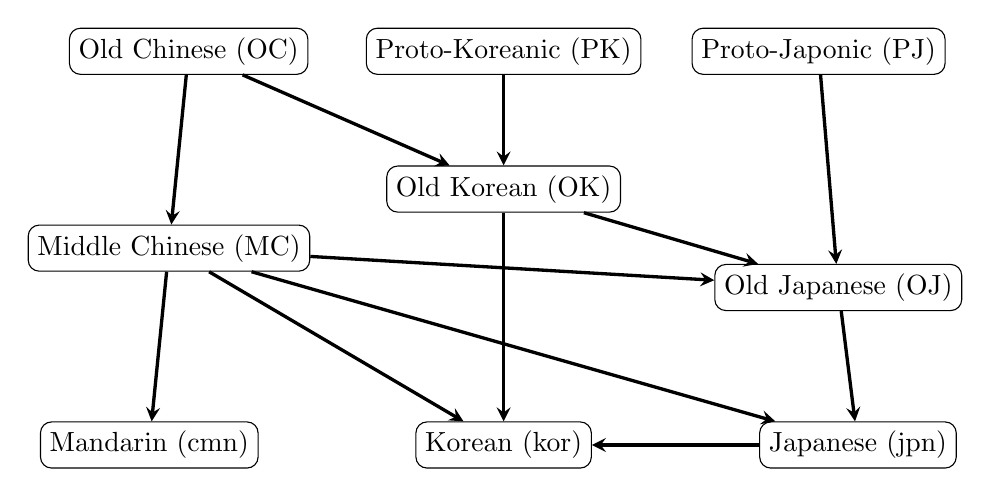
\begin{tikzpicture}
  [scale=.5,auto=left,every node/.style={shape=rectangle, rounded corners,
    draw, align=center}]
  \node (OC) at (1,11) {Old Chinese (OC)};
  \node (PK) at (9,11) {Proto-Koreanic (PK)};
  \node (PJ) at (17,11) {Proto-Japonic (PJ)};
  \node (MC) at (0.5,6) {Middle Chinese (MC)};
  \node (OK) at (9,7.5) {Old Korean (OK)};
  \node (OJ) at (17.5,5) {Old Japanese (OJ)};
  \node (cmn) at (0,1) {Mandarin (cmn)};
  \node (kor) at (9,1) {Korean (kor)};
  \node (jpn) at (18,1) {Japanese (jpn)};
  \begin{scope}[very thick, -stealth]
  \foreach \from/\to in {OC/MC,MC/cmn,PJ/OJ,MC/OJ,MC/jpn,MC/kor,OC/OK,PK/OK,OK/kor,OJ/jpn, OK/OJ,jpn/kor}
     \draw (\from) -> (\to);
  \end{scope}
  \end{tikzpicture}
 \caption{Example graph over (selected) languages of East Asia}
\label{fig:langGraph}
\end{figure}


As a final remark about conditional independence, it is worth emphasizing that conditioning on additional variables can not only remove dependencies, but it can also induce dependencies between otherwise independent variables. As stated earlier for our heating costs example, we are likely to observe an independence $(R \independent O)$ if we do not condition on anything else. However, this is only the case because people will regulate the heating to ensure a constant $R$. But any fixed investment $H$ into heating will be more or less effective at different outside temperatures. For fixed $H$, room temperature will therefore begin to depend on the outside temperature, so that we have a conditional dependence $(R \notindep O\ |\ H)$, whereas we had $(R \independent O)$. This is also the pattern underlying selection bias, which can be treated in the framework of conditional independence relations by introducing a hidden selection variable $S$, and assuming that the data are actually from the conditional 
distribution given $S$. This effectively turns every statement of the form $(X \notindep Y)$ into an underlying $(X \notindep Y\ |\ S)$, which does not contradict $(X \independent Y)$ in the underlying truth. 

Selection bias is a frequent problem in the application of statistical arguments within historical linguistics. For any linguist trying to prove that two groups of languages are related, it is difficult to avoid a natural tendency to filter the material in some way, e.g. by focusing on certain parts of the vocabulary that seem more promising. This becomes a problem as soon as statistical testing comes into play, where bias-free sampling is essential for estimating the amount of similarity that we would expect by chance, and therefore correctly determining the significance level. To illustrate that selection bias can also have an impact on purely data-driven approaches, assume that we want to assess by large-scale vocabulary comparison whether there is a hidden common ancestor between \ili{Basque} (\textit{eus}) and \ili{Albanian} (\textit{sqi}), such as a common Old European substrate. In a balanced sample of our vocabulary, we would very likely find $(eus \independent sqi)$. Now assume that we want to build the analysis on parallel word lists which include the oldest attested languages of Europe, such as \ili{Gothic} (\textit{got}). If the compiler of these word lists had any tendency to tune the selection of concepts towards those for which a Gothic word is known, e.g. in order to create a more fully populated table, the nature of the only available longer Gothic text (a Bible translation) will induce a selection bias. Both Basque and Albanian are heavily influenced in their religious vocabulary by \ili{Latin} and \ili{Romance languages}, which could easily lead to a statistically significant similarity on the word list $(eus \notindep sqi\ |\ got)$, even though we only considered data for the two languages, and might erroneously conclude that $(eus \notindep sqi)$. The same could happen in corpus-based approaches that rely on religious texts such as Bible translations, which are quite frequently the only available written records especially of smaller languages that do not have an indigenous writing tradition.

\subsection{Bayesian networks}
The more variables we consider, the more difficult it becomes to estimate and represent their joint distribution. However, if factorizations of the joint distribution function are possible, they can be used to build a directed acyclic graph (DAG) where each node contains the conditional probability distribution of one variable given a set of parent variables. The resulting \textit{Bayesian networks}\is{Bayesian network} provide a very compact way of representing joint distributions of many variables, and lend themselves very well to a range of important inference tasks. \cite{pearl1988} is the classical book on Bayesian networks, which explains many of the basic notions and issues in a very detailed and readable fashion, including the motivation of the following definitions.

Let $p(v)$ be the joint probability distribution on an ordered set $V = \{X_1,\dots,X_n\}$ of variables. A set $PA_j \subset V$ is said to be the \textit{Markovian parents} of a variable $X_j \in V$ if it is a minimal set of predecessors of $X_j$ that renders $X_j$ independent of all its other predecessors. In our East Asian example, $\{OJ,OC\}$ is not the set of Markovian parents of \ili{Japanese}, because according to the graph, this set does not explain all the overlap between \ili{Middle Chinese} and Japanese. Adding Middle Chinese to the set will still not give us the Markovian parents of Japanese, because the subset $\{MC,OJ\}$ already covers all paths from any other language into Japanese, and \ili{Old Chinese} is not a Markovian parent, because it is screened off by the other two languages in the set $\{MC,OJ\}$, which is therefore the set of Markovian parents of Japanese. Note that the situation could be different if we had chosen to model, say, Middle Japanese in addition, which would replace Old 
Japanese in the set of Markovian parents.

If a probability function $p$ admits the factorization $p(x_1,\dots,x_n) = \prod_i p(x_i\ |\ pa_i)$ relative to a DAG $G$, we say that $p$ and $G$ are \textit{(Markov) compatible}. In words, each variable must be independent of its non-descendants in the graph if the state of its Markovian parents is known. We say that a joint distribution fulfills the \textit{Markov condition}\is{Markov condition} if there is some graph to which it is compatible. As we have seen, the graph is mirrored by a factorization of the joint probability distribution, which can be used to compactly represent and efficiently perform calculations on joint and marginal probabilities.

Later textbooks such as \cite{koller_friedman_2009} build on a much more advanced theory and two decades of practical experience in applying graphical models to many problems. However, Bayesian networks have developed into a separate field which is mainly concerned with other tasks, such as the efficient inference of marginal distributions from joint distributions encoded as networks. This newer literature might therefore serve less well to lead the viewer towards an understanding of their importance for causal reasoning, a topic which we turn to in the next section.

\subsection{Causal interpretation of {B}ayesian networks}
From a philosophical angle, it appears attractive to give a causal interpretation to Bayesian networks, taking the directed arcs in Bayesian networks to represent direct causal influence of one variable on another. \cite{pearl2009} presents a range of ideas that follow from this viewpoint. Reinterpreting Bayesian networks not as convenient representations of joint probability distributions, but as causal DAGs which actually model the causal processes that generated the data, makes it possible to predict what happens if one of the variables is manipulated from the outside. Pearl develops this idea into a full intervention calculus, providing a framework for calculating answers to counterfactual questions as they arise in jurisdiction when, for instance, responsibility for an accident needs to be decided, and which previously were notoriously difficult to grasp mathematically. As Pearl shows, his fresh view of causality also provides a handle on long-standing statistical paradoxes like Simpson's paradox, where the direction of a correlation between two variables can revert in each individual case when we consider all values of a third value separately. Using the calculus of interventions with its true manipulation operation distinct from conditioning, the seeming paradoxes instantly disappear. As Pearl shows, they only existed due to a confusion of conditioning and manipulation, two operations which the classical statistical methods could not cleanly distinguish. By giving a causal interpretation to Bayesian networks, and thinking about experiments as manipulating the network, we gain a mathematical language for speaking about causality.

Stepping back from predicting the consequences of manipulation, the conditional independence relations we can extract from observational data can be exploited systematically to infer parts of the process which generated the data. This algorithmic side of causal analysis was further developed by \cite{spirtes_ea_2000}. Their book provides many of the technical proofs for the theory of inferred causation, and contains the first versions of several central algorithms which I will build upon in this book. It also provides a wealth of impressive examples, including a very in-depth discussion of how causal inference can be used on existing data to prove once and for all that smoking does cause lung cancer. The argument effectively destroys the tobacco industry's last line of defense, which consisted in claiming that the correlation might be due to a genetic predisposition which causes both a taste for cigarettes, and a propensity to develop lung cancer, an explanation which seems absurd, but cannot be ruled out by 
classical statistical methods.

In this book, I explore how this framework can be applied to languages. If we manage to model language graphs such as the East Asian example in \figref{fig:langGraph} as Bayesian networks, we can give a causal interpretation to the arrows, and should be able to use causal inference in order to infer the structure of the network which generated the observable data. If our observations consist of lexical data (as they do in this book), the causal graph can be interpreted as a minimal explanation of how the observed patterns could result from languages influencing each other, either by inheritance (as in the case of \ili{Old Chinese} and \ili{Middle Chinese}) or by borrowing (as in the case of \ili{Japanese} influence on \ili{Korean}). Each directed arc will represent the transmission of lexical material, and depending on how the underlying conditional independence tests are implemented, each link will correspond to a set of etymologies, detailing which words the model assumes to have been transmitted  along which path through the network.

Unfortunately, as we shall see, applying causal inference in practice to a new domain is a lot less straightforward and instantly rewarding than such examples would suggest. The proliferation of additional approximation tricks and processing steps in the literature is a tell-tale sign that one should never expect readily available implementations to yield useful results on a new problem, such as lexical flow modeling in my case. Still, most work on causal inference takes place within the confines of an almost canonical set of basic ideas and algorithmic procedures, and it is this core of the causal toolbox that I will be introducing throughout the rest of this chapter.

\section{Causal inference algorithms}\label{sec:3:2}
This section introduces the basics of \textit{causal inference} or \textit{causal discovery}, which is defined as the task to analyse a set of data (observations of three or more variables) to find a \textit{causal structure} (a partially directed acyclic graph) which mirrors the data-generating process as closely as possible. After laying out the basic assumptions and theorems which link conditional independence relations to constraints on the graph structure, I will give an overview of different approaches to testing for conditional independence, and then proceed to motivating and describing the most important causal inference algorithms. Pointers to the relevant literature will enable the reader to find proofs and more general variants of the various mathematical theorems which are needed to explain the motivation behind the algorithms, and why they work.

\subsection{Causal graphs}\label{sec:3.2.1}
I start by defining precisely the mathematical objects that I will be operating on. After defining different types of (partially) directed graphs which can be used to represent causal structures, and basic graph-theoretic notions which will be needed afterwards, I introduce the central notion of d-separation, and its generalization to ancestral graphs. Then, the main assumptions and theorems which link conditional independence relations and possible causal graphs are cited and put into context.

\subsubsection{Basic definitions}
A \isi{causal graph} $G = (V,E)$ consists of a set of nodes $V$ which represent random variables, and a set of edges $E \subset V \times V$ which will be taken to represent the causal connections between those variables. In the more general variant where the presence of hidden common causes and selection bias cannot be excluded, we have a partition $E = E_\rightarrow \cup E_\leftrightarrow \cup E_\text{---}$ into directed arcs which represent direct causal links, bidirected arcs which represent the existence of a hidden common cause for the two variables in question, and undirected arcs to represent the presence of selection bias inducing a dependence between two variables. For each of the three relation types, we will typically just write $X \text{ --- } Y$ for $(X,Y) \in E_\text{---}$, $X \rightarrow Y$ for $(X,Y) \in E_\rightarrow$, and $X \leftrightarrow Y$ for $(X,Y) \in E_\leftrightarrow$.

There is some convenient short-hand terminology which can be used to talk about the relations defined by the different edge types. For instance, the asymmetric directed arcs in $E_\rightarrow$ define the \textit{parent} relation\is{parent relation}, and in subsequent definitions I will write $pa(X) := \{Y \in V\colon (Y,X) \in E_{\rightarrow}\}$ ro refer to the set of parents of $X$.

A \textit{path}\is{path (in graph)} in a graph $G$ is a sequence $\langle X_0,\dots,X_n \rangle$ of distinct vertices $X_0,\dots,X_n$ where $(X_i,X_{i+1}) \in E$ for $0 \leq i < n$. If in addition, $(X_i,X_{i+1}) \in E_\rightarrow$ for all $0 \leq i < n$, we have a \textit{directed path}\is{directed path (in graph)} from $X_0$ to $X_n$. If there is directed path from $X$ to $Y$, or $X = Y$, $Y$ is called a \textit{descendant}\is{descendant (in graph)} of $X$, and $X$ an \textit{ancestor}\is{ancestor (in graph)} of $Y$. For the set of ancestors of any node $X \in V$, we will write $an(X)$. Applying this terminology to our example network of East Asian languages, there is a directed path from \ili{Old Chinese} to Mandarin\il{Mandarin Chinese}, but no directed path from \ili{Japanese} to Mandarin. Deviating from the standard terminology in historical linguistics, where every language has a single ancestor, and the recipient language of a layer of borrowings is not called a descendant of the donor language, in 
graph terminology Old Chinese is an ancestor of both Mandarin and Japanese, whereas Japanese is a descendant of both \ili{Old Japanese} and \ili{Middle Chinese}.

A \textit{\isi{directed cycle}} pattern exists whenever we have a directed path from $X$ to $Y$, but also a link $Y \rightarrow X$, allowing us to get back to the beginning of the path. Similarly, an \textit{\isi{almost directed cycle}} consists of a directed path $\langle X,\dots,Y \rangle$ and a bidirected arc $Y \leftrightarrow X$. In our East Asian language network, we do not have a directed cycle, and due to their temporal nature such cycles will not typically occur in language networks, unless we collapse different stages of three languages between which contacts in all directions have existed. For instance, if we did not treat \ili{Old Korean} (for which little lexical data is available) as distinct from Modern \ili{Korean}, we would get a directed cycle $OJ \rightarrow jpn \rightarrow kor \rightarrow OJ$. The existence of directed cycles in a lexical flow network will show us something was wrong with our data, and causal inference algorithms therefore assume that directed cycles will not occur.

If $E_\leftrightarrow$ and $E_\text{---}$ are empty, and there are no directed cycles in $E_\rightarrow$, $G$ is called a \textit{\isi{causal DAG}}. This type of structure is used to model situations in which \isi{causal sufficiency} holds, i.e.\ where there are no unobserved common causes which could act as confounders. In the presence of confounders, we will instead rely on \textit{ancestral graphs}\is{ancestral graph}, which do allow bidirectional links (nonempty $E_\leftrightarrow$), but do not contain any almost directed cycles, and additionally require that nodes connected by undirected edges $X_i - X_j$ do not have any parents, and are not connected to further nodes by $\leftrightarrow$ edges. The East Asian language network can be considered a causal DAG because all relevant causes of lexical overlap are explicitly modeled as nodes. If we had left out reconstructed languages such as \ili{Old Korean} and the two proto-languages, these would act as confounders, and the resulting structure could only be 
an ancestral graph.

Causal inference relies on certain configurations of directed and bidirected edges. Many of these configurations have special and mnemonic names. For instance, a pattern of the form $X \rightarrow Y \rightarrow Z$ is called a \textit{\isi{chain}} (e.g. $OC \rightarrow MC \rightarrow cmn$), and a pattern $X \leftarrow Y \rightarrow Z$, such as the pattern $kor \leftarrow MC \rightarrow jpn$, is called a \textit{\isi{fork}}.
Most importantly, a \textit{\isi{collider}} on a path is any node where arrow tips meet. In the directed graph case, colliders can only have the form $X \rightarrow Y \leftarrow Z$, such as in the pattern $MC \rightarrow jpn \leftarrow OJ$. In the more general case of ancestral graphs where bidirectional edges exist, the patterns $X \leftrightarrow Y \leftrightarrow Z$, $X \leftrightarrow Y \leftarrow Z$, and $X \rightarrow Y \leftrightarrow Z$ count as colliders just as well. An \isi{unshielded collider} or \textit{\isi{v-structure}} is a collider $X \rightarrow Y \leftarrow Z$ where $(X,Z) \notin E$. The five v-structures in the East Asian language network are $OC \rightarrow OK \leftarrow PK$, $OK \rightarrow OJ \leftarrow PJ$, $OK \rightarrow OJ \leftarrow MC$, $OK \rightarrow kor \leftarrow MC$, $OK \rightarrow kor \leftarrow jpn$. As we shall see throughout this book, the identifiability of v-structures is the cornerstone of constraint-based causal inference, because they are the source of all evidence 
of directionality.

\subsubsection{d-Separation}
To precisely capture the links between independence constraints and the graph structure, we will need the notion of \textit{\isi{d-separation}}. Intuitively, two variables are d-separated by a set of conditioning variables if every path by which information might flow from one node to the other through the graph, is blocked in some way by one of the variables we are conditioning on. In a directed graph, ways in which information flow can be blocked are a bit involved, so that a quite technical definition becomes necessary.

In Pearl's definition, a path $p$ in a DAG $G$ is said to be \textit{d-separated} by a set of nodes $\mathbf{Z}$ iff
\begin{enumerate}
  \item $p$ contains a noncollider, i.e.\ a chain $i \rightarrow m \rightarrow j$ or a fork $i \leftarrow m \rightarrow j$, with $m \in \mathbf{Z}$
  \item $p$ contains a collider $i \rightarrow m \leftarrow j$ such that $m \notin \mathbf{Z}$ and no descendant of $m$ is in $\mathbf{Z}$
\end{enumerate}
A set $\mathbf{Z}$ is said to d-separate $X$ from $Y$ iff $\mathbf{Z}$ d-separates every path from a node in $X$ to a node in $Y$. Paths and sets of nodes which are not d-separated are also called \textit{d-connected}.

To illustrate, let us first come back to the heating cost example, and consider the paths between household income $I$ and latitude $L$. We have assumed a path $I \arrowLA W \arrowAL O \arrowAL L$. This path is d-separated by the empty set $\{\}$ because it contains a collider. $\{W\}$ does not d-separate $I$ and $O$ because it contains the collider, but $\{O\}$ (in a chain) does. We have also assumed a second path $I \arrowLA W \arrowLA H \arrowAL O \arrowAL L$ which is d-separated by the empty set as well, but d-connected by $\{H\}$. The set $\{H\}$ also d-connects the first path because $H$ is a descendant of $W$. To summarize, both $\{W\}$ and $\{H\}$ d-connect the variables $I$ and $L$, whereas the set $\{O\}$ d-separates them because it d-separates both paths.

In the East Asian example network, \ili{Middle Chinese} and \ili{Old Korean} are d-separated by \ili{Old Chinese} because every other path between the two languages contains a collider. If we add \ili{Japanese} to the set $Z$, however, the two languages become d-connected, because now we have a path $OK \rightarrow OJ \leftarrow MC$ with a collider that gets unblocked because one of its descendants is in K. We thus have one d-connected path, which makes the two languages d-connected. To illustrate how this abstract reasoning corresponds to information flow, note that Old Korean and Middle Chinese will seem completely independent if we discard all the shared material from Old Chinese, e.g. by only looking at the lexical innovations in Middle Chinese, and checking whether they are reflected in Old Korean. However, if we additionally consider the loanwords from both languages in Japanese, we will find that if we determined a word in Japanese as not having existed in Middle Chinese, but we are sure that it 
already existed in Old Chinese, this will allow us to conclude that it must have been borrowed from \ili{Old Korean} via \ili{Old Japanese}, even if the word in question is not attested in any of the few sources in Old Korean. Knowledge of Middle Chinese starts to provide us with information about Old Korean, but only because both of these languages left traces in the lexicon of modern Japanese.

For the case where $G$ is an ancestral graph, \cite{richardson_spirtes_2002} introduce the more general notion of \textit{\isi{m-separation}}, which is identical to the definition of d-separation except that the more general definitions of collider and noncollider are used, where bidirected arrows are allowed. A \isi{maximal ancestral graph (MAG)} for a distribution $P$ then is an ancestral graph for $P$ with the additional property that for any pair of non-adjacent nodes there is a set by which they are m-separated. As we shall see, there is a direct correspondence between m-separation in $G$ and conditional independence relationships in $P$.

\subsubsection{Faithfulness}
To repeat the definition of a Bayesian network, a distribution $p$ fulfills the Markov condition with respect to a DAG $G$ if it factorizes according to the parent relationship defined by $G$, i.e.\ if $p(X_1,\dots,X_n) = \prod_{i=1}^k q(X_i\ |\ pa(X_i,G))$. If there is any such DAG, $p$ fulfills the \textit{\isi{Causal Markov Condition}}, one of the preconditions for constraint-based causal inference.

A distribution $p$ is called \textit{faithful to}\is{faithfulness} a DAG $G$ if the conditional independence relationships which hold in $p$ are exactly the ones implied by the d-separation criterion on $G$. We call the distribution $p$ as a whole \textit{faithful} if it is faithful to some DAG. This \textit{\isi{Causal Faithfulness Condition}} is the second precondition for causal inference. Informally, it ensures that there are no spurious independences which occur just because some numbers happen to cancel out perfectly. For instance, for an independence test based on vanishing partial correlation, this implies that the correlation must never become zero for a pair of dependent variables.

In the heating costs example, the previously determined d-separating sets on our paths $I \arrowLA W \arrowAL O \arrowAL L$ and $I \arrowLA W \arrowLA H \arrowAL O \arrowAL L$ imply that a distribution that is faithful to our scenario should show the conditional independence relationships $(I \independent L)$ and $(I \independent L\ |\ \{O\})$, but the conditional dependence $(I \notindep L\ |\ \{H\})$. Conditioning on $H$ is thus
predicted to induce a dependency between $I$ and $L$, which fits with our previous considerations because in a selection of households with identical heating costs, the richer households will tend to cluster in regions with lower latitudes, because the larger window panes of the rich will cause high heating costs even in less severe winters. As the constraints predicted by d-separation say, the dependence should disappear again if we additionally condition on $O$, because we then look at each region separately.

\subsubsection{(In)Dependence constraints and graph patterns}
Given faithfulness, a collider $A \rightarrow C \leftarrow B$ corresponds to the following two conditional (in)dependence constraints: $(A \independent B)$, but $(A \notindep B\ |\ C)$. We have seen this in the heating costs example, where the true pattern $W \rightarrow H \leftarrow R$ was reflected by the observations that $(R \independent W)$, the room temperature was independent of the window size, but $(R \notindep W\ |\ H)$, not for fixed heating costs.

In contrast, the fork $A \leftarrow C \rightarrow B$ as well as the chains $A \rightarrow C \rightarrow B$ and $A \leftarrow C \leftarrow B$ all correspond to  $(A \notindep B)$, but $(A \independent B\ |\ C)$. To distinguish between these possibilities, we would need additional variables and additional conditional independencies. This shows that conditional independencies alone do not completely determine causal structure. For instance, if we wanted to use conditional independence tests in order to decide which direction of borrowing is responsible for the shared lexical material between \ili{English} and \ili{Japanese}, we will not be able to do this based on data from another heavy recipient of English loanwords such as the Dravidian language \ili{Telugu} (\textit{tel}). We will find that $(tel \notindep jpn)$ due to shared loanwords from English, but that $(tel \independent jpn\ |\ eng)$, because these loanwords are the only source of lexical overlap between the two languages. In addition to the 
underlying fork $(tel \leftarrow eng \rightarrow jpn)$, this independence pattern could be due to a chain $(tel \rightarrow eng \rightarrow jpn)$ or a chain $(jpn \rightarrow eng \rightarrow tel)$, as long as we only take data from these three modern languages into account. This ambiguous configuration of (in)dependence constraints will appear very commonly when language isolates are involved.

So how much about the true graph can we determine from (in)dependence constraints? There are several central theorems in the literature which show that the relationship is rather close. Given causal sufficiency, for each faithful and Markovian probability distribution there is a DAG whose d-separation relationships correspond exactly to the conditional independencies in the distribution. Crucially for the inference task, it further turns out that the v-structures in a DAG $G$ alone fully determine the probability distributions that are compatible with G. If two graphs contain the same v-structures, causal inference cannot distinguish them, and they are Markov equivalent. Markov equivalence therefore partitions DAG structures into Markov equivalence classes\is{Markov equivalence}, the members of which cannot be distinguished by constrained-based causal inference. Each Markov equivalence class can be represented by a \textit{\isi{completed partially directed acyclic graph (CPDAG)}}, i.e.\ an acyclic graph where edges may be undirected, representing the fact that some of the Markov equivalent DAGs have an arrow in one direction on this edge, and some others have an arrow in the reverse direction.

In the absence of causal sufficiency, the correspondence between graph structure and independence constraints gets a little less direct. Again moving to the more complex case where latent common causes and selection bias might be present, we find that each Markov equivalence class of MAGs can be represented by a \textit{\isi{partial ancestral graph (PAG)}}. For an underlying DAG $G = (X \cup L \cup S,E_\rightarrow)$ over a set of observed variables $X$, a set of latent variables $L$, and a set of selection variables $S$, a PAG which represents $G$ is a graph $G' = (X, E')$ over $X$ with six edge types $\arrowLA$, $\arrowOA$, $\arrowOO$, $\arrowAA$, $\arrowLL$, and $\arrowOL$, if for every distribution $P$ that is faithful to $G$, we have
\begin{itemize}
 \item $(X_i,X_j) \notin E' \Rightarrow \exists Y \subseteq X \backslash \{X_i,X_j\}:\ (X_i \indep X_j\ |\ Y)_P$
 \item $(X_i,X_j) \in E \Rightarrow \forall Y \subseteq X \backslash \{X_i,X_j\}:\ (X_i \notindep X_j\ |\ Y)_P$
 \item $X_i \arrowLA X_j$ or $X_i \arrowOA X_j$ or $X_i \arrowAA X_j$ $\Rightarrow X_j \notin an(X_i,G')$
 \item $X_i \arrowLL X_j$ or $X_i \leftarrow X_j$ or $X_i \arrowOL X_j$ $\Rightarrow X_j \in an(X_i,G')$
\end{itemize}
This rather complex definition captures the type of graph structure we can optimally derive to approximate an underlying true causal graph, based only on conditional independence tests for a subset of observed variables. Whereas the definition of the arrow types $\rightarrow$ and $\leftrightarrow$ is as before, for the equivalence classes we additionally use the end symbol $\circ$ to designate uncertainty, such that $X_i \arrowLO X_j$ means ``$X_i \arrowLL X_j$ or $X_i \arrowLA X_j$'', and $X_i \arrowOA X_j$ means ``$X_i \arrowLA X_j$ or $X_i \arrowAA X_j$'' PAGs will be the output structures of the FCI and RFCI algorithms described in \sectref{sec:3.2.4}, which I will apply to language data in \chapref{sec:7}.

To characterize Markov equivalence classes of MAGs, and therefore the structures represented by PAGs, we need the definition of a special kind of path, which will later also play a role in PAG inference. A \textit{\isi{discriminating path}} for a vertex $V$ is a path $\langle X, \dots, W, V, Y \rangle$ of at least three edges, where $X$ and $Y$ are non-adjacent, and every vertex between $X$ and $V$ is a collider as well as a parent of $Y$.

Informally, a discriminating path provides an environment for a node $V$ which allows us to safely identify it as a collider even within a triangle. \cite{spirtes_richardson_1997} show that two MAGs are Markov equivalent if and only if they have the same undirected link structure and the same v-structures (i.e.\ are equivalent as CPDAGs), and furthermore have identical colliders among all nodes for which shared discriminating paths exist. Discriminating paths can therefore be seen as providing the environments in which unshielded colliders can safely be established, even in the presence of confounders.

\subsection{Determining conditional independence relations}\label{sec:3.2.2}
As we have seen in the previous section, any causal inference method which builds on inferring a causal graph from constraints will need a reliable way of deciding for any pair of observed variables $X$ and $Y$ whether they are dependent or not given different subsets $\mathbf{Z}$ of all observed variables. The reliability of these conditional independence tests are the main issue for the reliability of causal inference, because given perfect judgments, the theorems give us certainty that we will arrive at an equivalence class of correct structures. Causal inference algorithms mainly differ in how well they can recover from possible wrong conditional independence decisions.

\subsubsection{Testing for vanishing partial correlation}\label{sec:3.2.2.1}
The most straightforward statistical tests for conditional independence are based on testing for vanishing partial correlation. As \cite{baba_ea_2004} show, this is only guaranteed to work under the assumption that all involved variables are multivariate Gaussian, and does not provide us with a good test for other distributions, including discrete variables.

The \isi{Pearson correlation} coefficient $\rho_{XY}$ of two variables $X$ and $Y$ is defined as follows:
\begin{equation}
\rho_{XY} := \frac{Cov(X,Y)}{\sqrt{Var(X)}\cdot \sqrt{Var(Y)}}
\end{equation}
It is thus a normalization of the covariance $Cov(X,Y) := E[(X - E[X])(Y - E[Y)]$, which measures whether the two variables tend to deviate from their means in the same directions. We say that $X$ and $Y$ are \textit{correlated} if and only if $\rho_{XY} \neq 0$.

A conditional variant is defined by the \textit{\isi{partial correlation}} $\rho_{XY\cdot \mathbf{Z}}$, which is defined as the Pearson correlation $\rho_{R_XR_Y}$ of the residuals $R_X$ and $R_Y$ resulting from the linear regression of $X$ and $Y$ with $\mathbf{Z}$. For instance, to compute the residual $R_X$ for a vector of $n$ regression variables $\mathbf{Z} = \{Z_1,\dots,Z_n\}$ from $N$ observations, we need to find the $n$-dimensional coefficient vector $\mathbf{w}^{*}_X$ which optimizes the following minimization problem:
\begin{equation}
 \mathbf{w}^{*}_X = \argmin{\mathbf{w}} \left\{\sum_{i=1}^N (x_i - \langle \mathbf{w}, \mathbf{z_i} \rangle)^2 \right\}
\end{equation}
The observations of the residual $R_X$ are then $x_i - \langle \mathbf{w}^{*}_X, \mathbf{z_i} \rangle$ for $1 \leq i \leq N$,
from which we can compute the Pearson correlation with the analogous residual $R_Y$.

A more direct alternative is to compute $\rho_{XY\cdot \mathbf{Z}}$ via a recursive formula, which uses several partial correlations of lower order to compute one partial correlation of higher order, with Pearson correlation as the base case. For any $Z_0 \in \mathbf{Z}$, we have:
\begin{equation}
 \rho_{XY\cdot \mathbf{Z}} = 
 \frac{\rho_{XY\cdot \mathbf{Z}\backslash\{Z_0\}} - \rho_{XZ_0\cdot \mathbf{Z}\backslash\{Z_0\}} \rho_{Z_0Y\cdot \mathbf{Z}\backslash\{Z_0\}}}
      {\sqrt{1-\rho^2_{XZ_0\cdot \mathbf{Z}\backslash\{Z_0\}}} \sqrt{1-\rho^2_{Z_0Y\cdot \mathbf{Z}\backslash\{Z_0\}}}}
\end{equation}

To test for vanishing partial correlation in order to establish conditional independence,
\citet[5.5]{spirtes_ea_2000} use Fisher's z-transform of the partial correlation $\hat{\rho}_{XY\cdot \mathbf{Z}}$ in the sample:
\begin{equation}
 z(\hat{\rho}_{XY\cdot \mathbf{Z}}) := \frac{1}{2} \ln\left(\frac{1 + \hat{\rho}_{XY\cdot \mathbf{Z}}}{1 - \hat{\rho}_{XY\cdot \mathbf{Z}}} \right)
\end{equation}
If $N$ is the sample size, $\sqrt{N - |\mathbf{Z}| - 3} \cdot z(\hat{\rho}_{XY\cdot \mathbf{Z}})$ roughly approximates a standard normal distribution if the null hypothesis $\hat{\rho}_{XY\cdot \mathbf{Z}} = 0$ holds. To see whether the vanishing correlation assumption can be rejected, we thus test whether we have $\sqrt{N - |\mathbf{Z}| - 3} \cdot |z(\hat{\rho}_{XY\cdot \mathbf{Z}})| > \Phi^{-1}(1 - \frac{\alpha}{2})$ for the cumulative distribution function $\Phi$ of the standard normal distribution. This is the default option for conditional independence tests implemented in the R package \texttt{pcalg} by \cite{kalisch_ea_2012}.

\subsubsection{Testing for independence in the discrete case}\label{sec:3.2.2.2}
\citet[5.5]{spirtes_ea_2000} also describe standard procedures for conditional independence tests in the discrete case. If we see each cell count $x_{ij}$ in a table resulting from $N$ samples of two variables $X_i$ and $X_j$ as one multinomially distributed variable, the expected value of $x_{ij}$ under the independence assumption is $E(x_{ij}) = \frac{\sum_j x_{ij} \cdot  \sum_i x_{ij}}{N}$. If we add a third variable $X_k$ for which $(X_i \indep X_j\ |\ X_k)$, the corresponding cell $x_{ijk}$ will have the expected value $E(x_{ijk}) = \frac{\sum_j x_{ijk} \cdot  \sum_i x_{ijk}}{\sum_{i,j} x_{ijk}}$. Analogously, for $n$ conditioning variables $X_{k_1}, \dots, X_{k_n}$, we get
\begin{equation}
 E(x_{ijk_1\dots k_n}) = \frac{\sum_j x_{ijk_1\dots k_n} \cdot  \sum_i x_{ijk_1\dots k_n}}{\sum_{i,j} x_{ijk_1\dots k_n}}
\end{equation}

These expected cell counts can be tested against the observed values using standard tests. Under the independence assumption, the following two test statistics are both $\chi^2$-distributed for an appropriate number of degrees of freedom $df$:
\begin{equation}
 \chi^2 := \sum_{i,j,k_1,\dots,k_n} \frac{(x_{ijk_1\dots k_n} - E(x_{ijk_1\dots k_n}))^2}{E(x_{ijk_1\dots k_n})}
\end{equation}
\begin{equation}
 G^2 := 2 \cdot \sum_{i,j,k_1,\dots,k_n} x_{ijk_1\dots k_n} \ln \left( \frac{x_{ijk_1\dots k_n}}{E(x_{ijk_1\dots k_n})} \right)
\end{equation}
In principle, the degrees of freedom for a test of the conditional independence $(X_i \indep X_j\ | X_{k_1}, \dots, X_{k_n})$
can be computed from the number of categories $Cat$ for each variable as follows:
\begin{equation}
 df = (Cat(X_i) - 1) \cdot (Cat(X_j) - 1) \cdot \prod_{i=1}^{n} Cat(X_{k_i})
\end{equation}
This number is exponential in the number of conditioning variables, which will quickly lead
to zero entries in the table that need to be corrected for. In the absence of a general rule,
$df$ can be reduced by one for each zero entry as a rough heuristic.

\subsubsection{Testing for vanishing conditional mutual information}\label{sec:3.2.2.3}
A more general criterion for conditional independence stems from information theory, a branch of mathematics that is concerned with quantifying information and information flow. I will repeat the essential concepts of information theory here to provide some degree of self-containedness. The first chapters of any introductory textbook of information theory will introduce the same concepts with a lot more rigour and detail, also motivating the theory using a wealth of examples. For my purposes in this book, it satisfies to say that information theory will provide us with the mathematical tools for modeling languages as variables, and for defining the conditional independence tests that we will need to apply causal inference. The definitions as I state them in the following are adapted from \cite{cover_thomas_2006}.

The central concept of information theory is called \textit{\isi{entropy}}, and can be seen as a measure of the expected amount of information provided by a single outcome of (or alternatively, the uncertainty contained in not knowing the outcome of) a random variable $X$. In the discrete case (to which we will confine ourselves here), the entropy $H(X)$ of a discrete variable $X$ with the set of possible outcomes $\Omega(X)$ is defined as
\begin{equation}
 H(X) := - \sum_{x \in \Omega(X)} p(x) \log p(x)
\end{equation}

The entropy of a discrete variable $X$ can be seen as the average information content of a single observation of that variable, or as the expected value of the \textit{\isi{self-information}} $I(x) := - \log p(x)$ associated with an event $\{X = x\}$. Self-information is also called \textit{surprisal} because it measures the unexpectedness (or amount of surprise) associated with the observation that $X$ has the value $x$.

If we observe two information sources $X$ and $Y$ at the same time, some of the information we receive might coincide, which means that we cannot just add up the amount of information received by both sources to quantify our overall information. Instead, we generalize entropy to \textit{\isi{joint entropy}} $H(X,Y)$:
 \begin{equation}
  H(X,Y) = -\sum_{x} \sum_{y} p(x,y) \log p(x,y)
 \end{equation}
The amount of information we receive twice when jointly observing two information sources can be recast as the information
that one variable $Y$ provides about the state of the other variable $X$. This symmetric measure
is called the \textit{\isi{mutual information}} $I(X;Y)$:
 \begin{equation}
  I(X;Y) := H(X) + H(Y) - H(X,Y) = \sum_{y} \sum_{x} p(x,y) \log \left( \frac{p(x,y)}{p(x)p(y)} \right) 
 \end{equation}
Returning to individual events, we can define mutual information as the expected value of the \textit{\isi{pointwise mutual information}} $pmi(x;y)$
between two observations:
 \begin{equation}
  pmi(x;y) := \log \left( \frac{p(x,y)}{p(x)p(y)} \right) 
 \end{equation}
Pointwise mutual information is very useful for quantifying the strength of associations between
pairs of variable values. In \sectref{sec:4.4}, I will get back to PMI as a standard measure 
of association between sounds in models of sound correspondences.

Finally, we can measure the information which two variables $X$ and $Y$ provide about each other provided that the values of a set of certain other variables $\mathbf{Z}$ is known. This is called the \textit{\isi{conditional mutual information}} of $X$ and $Y$ given $\mathbf{Z}$:
 \begin{equation}
  I(X;Y|\mathbf{Z}) := \sum_{\mathbf{z}} p(\mathbf{z}) \sum_{y} \sum_{x} p(x,y|\mathbf{z}) \log \left( \frac{p(x,y|\mathbf{z})}{p(x|\mathbf{z})p(y|\mathbf{z})} \right) 
 \end{equation}
As \cite{yeung2008} demonstrates, it is easy to derive the following formula for computing conditional mutual information from joint entropies:
\begin{equation}
 I(X;Y|\mathbf{Z}) = H(X,\mathbf{Z}) + H(Y,\mathbf{Z}) - H(X,Y,\mathbf{Z}) - H(\mathbf{Z})
\end{equation}
The decisive property of mutual information for causal inference is that for joint distributions that are faithful to some causal graph, it provides us with a necessary and sufficient criterion for independence:
\begin{equation}
 X \indep Y \Leftrightarrow I(X;Y) = 0.
\end{equation}
More importantly for my application, this also extends to conditional mutual information, giving us the following characterization:
\begin{equation}
 (X \indep Y\ |\ Z) \Leftrightarrow I(X;Y|Z) = 0.
\end{equation}
Intuitively, this means that two sets of variables are independent given a third set of variables if and only if there is no information flow between the first two sets that could not be mediated by variables from the third set.

Given this equivalence, an obvious idea for implementing a very general independence test now is to check for vanishing mutual information. The problem with mutual information is, however, that it is hard to compute or estimate for any interesting type of variable. This means that to exploit this characterization of independence, we need to rely on other more easily computable measures which in all relevant respects behave just like joint entropy.

Assume we have a set of $n$ discrete random variables $X_1,\dots,X_n$ with the index set $[n] := \{1,\dots,n\}$. Then, the criteria for a real-valued function $h$ on subsets of $[n]$ to behave sufficiently like the joint entropy $H$ can be cast into three axioms that are known as the \textit{\isi{elemental inequalities}}, and are quoted here as in \cite{chaves_ea_2014}:

For all $S \subset [n] \backslash \{i,j\}, i \neq j,\ i,j \in [n]$:
\begin{itemize}
 \item $h([n] \backslash \{i\}) \leq h([n])$ (\isi{monotonicity})
 \item $h(S) + h(S \cup \{i,j\}) \leq h(S \cup \{i\}) + h(S \cup \{j\})$ (\isi{sub-modularity})
 \item $h(\emptyset) = 0$
\end{itemize}
Intuitively, the monotonicity condition ensures that uncertainty never becomes smaller if we consider a larger set of variables, and the sub-modularity condition ensures that the conditional mutual information derived from the entropy-like measure is always positive.

Together, these inequalities define an outer approximation to the region of vectors in the space of set functions $R_n$ which define some entropy function on all subsets of a set of $n$ discrete random variables. In less technical terms, this means that any set function for which the elemental inequalities hold is close enough in behaviour to entropy that we can use it to derive a consistent measure of conditional mutual information. For more background on this, the reader is referred to \citet[Ch. 14]{yeung2008}.

As we will see in \chapref{sec:6}, it is relatively straightforward to define measures for which the elemental inequalities hold. Based on a function which can in this regard be seen as a measure of entropy, this will make it possible to establish consistent (if unreliable) independence tests between sets of languages.

\subsection{The PC algorithm}\label{sec:3.2.3}
The first feasible and complete causal inference algorithm based on conditional independence tests is the PC algorithm as presented by \cite{spirtes_ea_2000}. This algorithm is a basic building block for many more recent approaches, and is the cornerstone for any understanding of constraint-based causal inference.

\subsubsection{Preconditions and assumptions}
The correctness and completeness of the PC algorithm depends on two very natural conditions, which are however only rarely met in applications to practical problems, and have therefore been weakened for later algorithms which build on the same basic principles.

The first prerequisite is the already mentioned causal sufficiency, i.e.\ we must assume that there are no unobserved common causes which act as confounders. If we try to circumvent this by operating with DAGs in which some nodes are unobserved, we quickly run into the problem that there are many DAGs over both observed and latent variables for which no equivalent DAG over only the observed variables exist, i.e.\ the Markov condition breaks down. The minimal example of this is a causal graph of the shape $X_1 \arrowAL L_1 \arrowLA X_2 \arrowAL L_2 \arrowLA X_3$, where $L_1$ and $L_2$ are unobserved. It is not possible to provide a DAG structure over $X_1$, $X_2$, and $X_3$ which corresponds by d-separation to the conditional independence constraints encoded in the larger structure. This will turn out to be a problem in my application, because this pattern is one of the most frequent among languages whenever two language families come into contact, e.g. in the configuration $deu \leftarrow Germanic \rightarrow fin \leftarrow Uralic \rightarrow yrk$, where \ili{Finnish} (\textit{fin}) is a Uralic language\il{Uralic languages} which was influenced by Germanic\il{Germanic languages}, unlike Eastern Uralic languages like \ili{Nenets} (\textit{yrk}).

The second prerequisite is faithfulness, which we already encountered in the context of defining the correspondence between independence constraints and the graphs they characterize. If the independence tests are too unreliable, and produce a pattern of independence constraints that violates faithfulness, this can be expected to mislead the algorithm, possibly to the point where it derives contradictory constraints which do not correspond to any causal structure.

\subsubsection{Basic version}
The basic architecture of the PC algorithm consists of three phases. In the first phase (Stage I), conditional independence tests are systematically performed to establish an undirected \textit{\isi{causal skeleton}}. For each pair of variables $A$ and $B$, we search for a minimal \textit{\isi{separating set}} $S_{AB}$ with $(A \independent B\ |\ S_{AB})$ (minimal in the sense that $(A \notindep B\ |\ S)$ for any $S \subset S_{AB}$). By doing so for every pair of variables, we construct an undirected graph $G$ with $\{A,B\} \in E$ whenever no such $S_{AB}$ could be found. The one observation which makes the PC algorithm tractable even for dozens of variables is that we do not need to test all possible separating sets $S_{AB}$ when attempting to separate $A$ and $B$. Instead, we can look for separating sets by increasing size, first removing all links between variables which are unconditionally independent from an initially complete graph, then all links which are independent given separating sets $S_{AB}$ of size 1, and so on.

In addition, two nodes $X_i$ and $X_j$ are d-separated in a DAG $G$ if and only if they are d-separated by either $pa(X_i,G)$ or $pa(X_j,G)$. Therefore, it suffices to check whether two variables are independent given their neighbors in order to check whether they are conditionally independent given any set of variables. As the graph gets sparser by the removal of links, so does the number of neighbors of $A$ and $B$ which the separating set $S_{AB}$ must consist of, which tends to make checking for all possible $S_{AB}$ tractable even for large set sizes.

In the next phase (Stage II), we check for the presence of v-structures. For each triple $A,B,C \in V$ with $\{A,B\} \notin E$, but $\{A,C\},\{B,C\} \in E$ (i.e.\ each \textit{\isi{unshielded triple}}), we add arrowheads pointing at $C$ (leading to a v-structure $A \rightarrow C \leftarrow B$) if $C \notin S_{AB}$. This inference is justified by the relationship between graph patterns and (in)dependence constraints established above. There is a v-structure $A \rightarrow C \leftarrow B$ if and only if we have $(A \independent B)$, but $(A \notindep B\ |\ C)$.  $(A \independent B)$ is given because we have an unshielded triple, without a direct causal connection between $A$ and $B$. The absence of $C$ in the separating set $S_{AB}$ implies that $(A \notindep B\ |\ C)$, because otherwise we would have found $S'_{AB} = \{C\}$ as a separating set before encountering $S_{AB}$. We infer the existence of a collider $A \rightarrow C \leftarrow B$ because all non-collider configurations would have led to $(A \independent B\ |\ C)$.

If our independence tests were completely reliable (and this is what the basic PC algorithm assumes), we can be sure that we have found exactly the correct v-structures at Stage II. This allows us to orient many of the remaining undirected edges (which were not part of any v-structure) in a third phase (Stage III), by repeatedly applying two simple criteria until no additional arrows can be inferred. If one direction of a link would lead to a new v-structure which was not detected at Stage II, we can add the arrow in the reverse direction (leading to a chain). Moreover, if we assume acyclicity (as implied by the Causal Markov condition), we can also orient any arrow where the reverse orientation would result in a cycle $A \rightarrow B_1 \rightarrow B_2 \rightarrow \dots \rightarrow A$. Enforcing the two principles can be achieved by applying four arrow propagation rules, which I will not cite here because they are subsumed by the ruleset of the more complex FCI algorithm in \sectref{sec:3.2.4}. Thanks to a proof by \cite{meek1995}, it has long been known that application of these four rules until the fixed point (until they do not apply any more) suffices to arrive at the CPDAG representing the Markov equivalence class of the true graph, i.e.\ containing all the arrows which are common to the causal graphs in the class. This even holds if we add background knowledge in the form of pre-directed arrows, as one would do if e.g.\ the temporal order makes the directionality of causation obvious.

\begin{figure}\small
\begin{minipage}{.23\textwidth}
  \begin{center}
   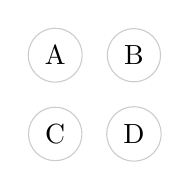
\begin{tikzpicture}
  [scale=.5,auto=left,every node/.style={circle,draw=black!20}]%{circle,border=black!20}]
  \node (v1) at (1,3) {A};
  \node (v2) at (3,3) {B};
  \node (v3) at (1,1) {C};
  \node (v4) at (3,1) {D};
  \end{tikzpicture}

  Conditional independence relationships:\\
  $(A \independent B\ |\ D)$\\
  $(A \independent B\ |\ C,D)$\\
  $(A \independent D\ |\ B,C)$\\
  \end{center}
\end{minipage}  
\begin{minipage}{.25\textwidth}
  \begin{flushleft} Stage I:
  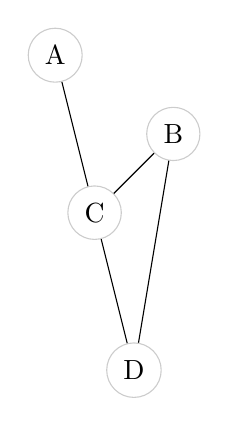
\begin{tikzpicture}
  [scale=.5,auto=left,every node/.style={circle,draw=black!20}]%{circle,border=black!20}]
  \node (v1) at (1,11) {A};
  \node (v2) at (4,9) {B};
  \node (v3) at (2,7) {C};
  \node (v4) at (3,3) {D};

  \foreach \from/\to in {v1/v3,v2/v3,v2/v4,v3/v4}
     \draw (\from) -- (\to);
  \end{tikzpicture}\\
  $S_{AB} = \{D\}$\\
  $S_{AD} = \{B,C\}$\\
  no further minimal separating sets found
  \end{flushleft}
\end{minipage}  
\begin{minipage}{.23\textwidth}
  \begin{flushleft} Stage II:
  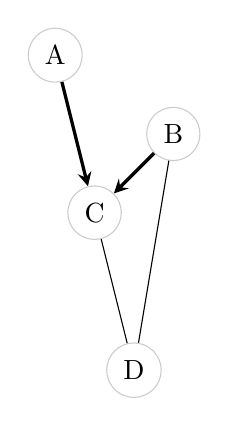
\begin{tikzpicture}
  [scale=.5,auto=left,every node/.style={circle,draw=black!20}]%{circle,border=black!20}]
  \node (v1) at (1,11) {A};
  \node (v2) at (4,9) {B};
  \node (v3) at (2,7) {C};
  \node (v4) at (3,3) {D};

  \foreach \from/\to in {v2/v4,v3/v4}
    \draw (\from) -- (\to);
    
  \begin{scope}[very thick, -stealth]
  \foreach \from/\to in {v1/v3,v2/v3}
    \draw (\from) -> (\to);
  \end{scope}
  \end{tikzpicture}\\
  ACD: $C \in S_{AD}$,\\ no arrows\\
  ACB: $C \notin S_{AB}$,\\ i.e.\ $A \rightarrow C \leftarrow B$
   \end{flushleft}
\end{minipage}  
\begin{minipage}{.23\textwidth}
  \begin{flushleft} Stage III:
  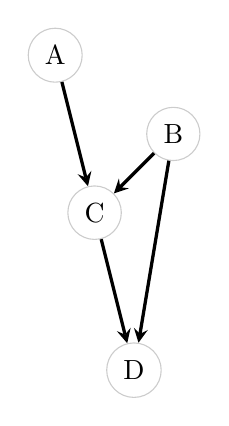
\begin{tikzpicture}
  [scale=.5,auto=left,every node/.style={circle,draw=black!20}]%{circle,border=black!20}]
  \node (v1) at (1,11) {A};
  \node (v2) at (4,9) {B};
  \node (v3) at (2,7) {C};
  \node (v4) at (3,3) {D};
  \begin{scope}[very thick, -stealth]
    \foreach \from/\to in {v1/v3,v2/v3,v2/v4,v3/v4}
    \draw (\from) -> (\to);
  \end{scope}  
 \end{tikzpicture}\\
  $C \rightarrow D$, otherwise new v-structure\\
  $B \rightarrow D$, otherwise directed cycle
   \end{flushleft}
\end{minipage}
\caption{Illustrating the phases of the basic PC algorithm}
\end{figure}

The result computed by the PC algorithm is the minimal graph structure whose d-separation relationships correspond exactly to the conditional independencies in the distribution, i.e. it will contain all those links which we must assume in order to explain the conditional independence properties of the data, and not a single additional link which would not be necessary. A procedure like the PC algorithm therefore implements Occam's razor, the scientific principle which requires us to pick among adequate explanations the one for which we need to make the smallest number of assumptions. The central role of Occam's razor is reflected by the importance of avoiding overfitting in machine learning, where it is typically possible to perfectly model the observable data using a complex model with many parameters (e.g. a fully connected graph), but due to the more difficult inference task, complex models are less likely to classify unseen examples well. It therefore makes sense for inference algorithms to infer the least complex model which still fits the observable data, and this is what the PC algorithm does for joint distributions of causally sufficient sets of variables.

\subsubsection{More recent variants}
The vanilla PC algorithm as I just presented it takes an unnecessary risk in selecting the neighbors out of which separating set candidates are formed. If the distribution is faithful to some DAG, $(A \indep B\ |\ pa(A))$ implies that $A$ and $B$ are independent given a set of nodes lying on undirected paths between $A$ and $B$. Conditioning on variables that are not on any connecting path will not cause any blockage of information flow. Therefore, it suffices to include only nodes on connecting paths in separating set candidates. \citet[5.4.2.3]{spirtes_ea_2000} call this modification the \textit{\isi{PC* algorithm}}, but advise shifting to the more exact separating set candidate selection criterion only after the graph was already thinned out, due to the high memory overload involved in maintaining a list of all connecting paths between any pair of nodes. I will be using a similar idea in \chapref{sec:6}, where the shape of my data allows me to adapt an explicit flow criterion for prefiltering the possible 
separating sets.

A major problem of the vanilla PC algorithm as well as its PC* variant is that the results can vary widely depending on the order in which separating sets are tried out, because the first one will be picked even though there might be many separating sets of the same minimal size. The \textit{Conservative PC} variant\is{Conservative PC algorithm} by \cite{ramsey_ea_2006} differs in not stopping as soon as a single sepset was found, but checking whether the middle variable is present in all or no separating sets of the current size. Unshielded triples where the relevant variable is contained in some, but not all separating sets, are not oriented as colliders, but marked as ambiguous, and prevented from taking part in the propagation rules. This rule will prevent uncertain directionality information from being propagated, but will often leave many edges unoriented.

The \textit{Stable PC} algorithm\is{Stable PC algorithm} by \cite{colombo_maathuis_2014} uses a majority rule to resolve this problem. This variant decides whether to orient each triple as a collider by counting the ratio of all minimal separating sets which contain $B$. Both conservativity and the majority rule remove the order-dependence in the presence of conflicting information, but the PC variants defined in this way still tend to yield either unstable or uninformative results, and must be re-run with different thresholds to detect the stable links.

\subsection{The FCI algorithm}\label{sec:3.2.4}
The FCI algorithm can be seen as a generalization of the PC algorithm to the situation where hidden common causes for some of the observed variables might exist. Such connections will be represented by the bidirected arrows (the edge set $E_\leftrightarrow$) in ancestral graphs.

\subsubsection{Basic version}
The original version of the \textit{FCI (Fast Causal Inference)} algorithm\is{FCI algorithm} was given by \cite{spirtes_ea_2000} as a variant of the PC algorithm in the absence of causal sufficiency. Much as the PC algorithm generates a CPDAG with the goal of approximating the underlying true DAG up to Markov equivalence, the FCI algorithm generates a PAG to represent the Markov equivalence class of the underlying true ancestral graph.

The basic procedure of FCI remains to systematically find separating sets for pairs of observed variables, thinning out a fully connected initial graph until we arrive at a skeleton which only connects pairs of variables that cannot be made independent by conditioning on any combination of the other variables. What makes the FCI algorithm much more complicated than the PC algorithm is that due to the possible existence of latent variables, we cannot assume that we can form a separating set for all pairs of m-separated variables from the neighbors in the current skeleton. To see this, consider the following minimal example taken from \citet[p.129]{spirtes_ea_2000}. We have two pairs of variables $A,B$ and $D,E$, each of which are dependent due to a hidden common cause. The only direct causal influence on $A$ among observed variables is $D \rightarrow A$, and the only influence on $E$ is $B \rightarrow E$. Assume further that neither of the variables $A,B,D,E$ has a direct causal influence on any other 
variable, observed or unobserved, and that there is an additional causal pattern $B \leftarrow F \leftarrow C \rightarrow H \rightarrow D$. This pattern induces a dependence $(A \notindep E)$, but the independence $(A \indep E\ |\ \{B,C,D\})$. There is a separating set which would allow us to delete the link, but this sets includes a variable which is not directly adjacent to either $A$ and $E$ in the true graph.

The question which sets we need to test in order to ensure that a pair of variables $X$ and $Y$ is not m-separated by any subset of the observed variables gives rise to the notion of an \textit{inducing path}. For two disjoint sets $L$ (latent variables) and $S$ (selection variables) of nodes in an ancestral graph which do not contain $X$ or $Y$, an \isi{inducing path} relative to $\langle L,S \rangle$ is a path between $X$ and $Y$ where every intermediate node is either a collider or in $L$, and every collider on the path is either in $S$ or an ancestor of $X$ or $Y$. A crucial result by \cite{richardson_spirtes_2002} shows that $X$ and $Y$ need to be connected in the true ancestral graph (are not m-separated by $Z \cup S$ for any $Z$ disjoint from $L$ and $S$) if and only if there is an inducing path from $X$ to $Y$ relative to $\langle L,S \rangle$.

For the systematic independence tests that are performed to arrive at a skeleton, the original version of the FCI algorithm relied on the notion of an inducing path graph, which, however, turned out \citep{zhang2006} to be less informative than the variant based on ancestral graphs, which is the only one that will be presented here.

After generating an initial skeleton just as in the first phase of the PC algorithm, we cannot yet be sure that all the pairs of still connected variables are actually m-connected in the true ancestral graph, because looking for separating sets only among the neighbors was sufficient to determine d-separation, but does not reliably check for m-separation. Some additional edges might have to be removed, and this is where the inducing path criterion comes in. If we partially orient the links in the initial skeleton by detecting v-structures, many of the paths in the skeleton between each pair of nodes $X$ and $Y$ cannot correspond to inducing paths in the underlying ancestral graph, whereas other might. It therefore suffices to check whether $(X \indep Y\ |\ Z)$ for each combination $Z$ of nodes $Z_k$ connected to $X$ by what might still represent an inducing path. If we manage to break every possible inducing path between the observed variables $X$ and $Y$ in this way, the inducing path criterion allows us to 
remove the link between $X$ and $Y$. In practice, the criterion used to find candidates $Z_k$ in the absence of latent variables checks whether each triple on the path forms either an unshielded collider or a triangle, which is the observable equivalent of an underlying inducing path.

In order to infer the directionality of links in the final skeleton, FCI again relies on the same basic procedure as the PC algorithm, after discarding the directionality information which was used to determine the final skeleton. After redetermining the v-structures as starting points, propagation rules are repeatedly applied, adding partial orientations to additional edges until no further changes occur. The four propagation rules given by \cite{spirtes_ea_2000} have the advantage of still being quite intuitive, but this first version of FCI did not aim to achieve completeness in the sense that it did not necessarily output the most specific maximal ancestral graphs.

\cite{zhang2008} closes this gap by developing and proving the completeness of a rather complex set of orientation rules, giving rise to the \isi{Augmented FCI (AFCI) algorithm}. Since this is the version of the rules which is used in my implementation of RFCI (see below), I will provide each rule here, and give an informal explanation of the intuition behind each of them, as well as their status in the overall inference system. For a compact notation of the conditions under which the rules apply, a star is used as an additional wildcard symbol to represent any arrow end state. This is different from the circle in that the circle represents a concrete state with the potential of being turned into an arrow or a line, whereas the star does not correspond to an actual state, and is only used to keep rule notations compact by matching any possible end symbol.

The first four rules ensure arrowhead completeness, i.e.\ they detect any arrowhead that is present in all members of the Markov equivalence class, based on the assumption that the inferred v-structures are correct. These rules are quite similar to the orientation rules used by the PC algorithm, with one additional rule that looks for discriminating paths which help to distinguish the configurations $A \leftrightarrow B \leftrightarrow C$ and $A \leftrightarrow B \rightarrow C$ in some cases:
\begin{itemize}
 \item $\mathcal{R}1:$ orient unshielded $A \arrowSA B \arrowOS C$ as $A \arrowSA B \rightarrow C$
 \item $\mathcal{R}2:$ orient $A \arrowSO C$ as $A \arrowSA C$ if $A \rightarrow B \arrowSA C$ or $A \arrowSA B \rightarrow C$ 
 \item $\mathcal{R}3:$ orient $D \arrowSO B$ as $D \arrowSA B$ if there is a pair of variables $A$ and $C$ with $(A,C) \notin E$
 which is in configurations $A \arrowSA B \arrowAS C$ and $A \arrowSO D \arrowOA C$
 \item $\mathcal{R}4:$ on a discriminating path $\langle D, \dots, A,B,C \rangle$,
 orient $B \arrowSO C$ as $B \rightarrow C$ if $B$ is in the separating set found for $D$ and $C$,
 and add arrows to form $A \leftrightarrow B \leftrightarrow C$ otherwise
\end{itemize}
Intuitively, the first rule $\mathcal{R}1$ exploits the assumption that in the previous step of the algorithm, we have found exactly the v-structures which are present in the true ancestral graph. This means that we can exclude any arrow that would lead to an additional collider, giving us additional chains. $\mathcal{R}2$ enforces the absence of almost directed cycles in the ancestral graph.

$\mathcal{R}3$ provides a way to infer additional arrows within shielded triples. If in the configuration it acts upon, we added an arrow from $B$ to $D$, the second rule would force us to assume $A \arrowSA D$ in order to avoid a cycle; in the unshielded triple $A \arrowSA D \arrowOS C$, the requirement not to introduce additional v-structures would force an additional arrow $D \rightarrow C$, leading to an (almost) directed cycle $B \rightarrow D \rightarrow C \arrowSA B$, which cannot exist. Therefore, the arrow $D \arrowSA B$ is the only option in this configuration. This inference by contradiction cannot be 
emulated by propagation rules.

The intuition behind $\mathcal{R}4$ is that discriminating paths show some of the behavior of unshielded triples, because on a discriminating path from $X$ to $Y$, the colliders are exactly the nodes which do not occur in any m-separating set for $X$ and $Y$, and the non-colliders are the nodes which occur in every such set. This property allows additional inferences of directionality, much in the same vein as the initial detection of v-structures, but in the presence of bidirectional arcs.

The second block of rules serves to infer the existence of line ends, i.e.\ they are
the overall system's way of detecting selection bias (undirected edges). If we can safely assume that no selection bias is present, these rules will never apply, and can thus safely be ignored:
\begin{itemize}
 \item $\mathcal{R}5:$ orient $A \arrowOO B$ 
 and all edges on an uncovered circle path $\langle A,C,\dots,D,B\rangle$
 where $(A,D) \notin E$ as well as $(B,C) \notin E$ as undirected (\arrowLL), if such a path exists
 \item $\mathcal{R}6:$ orient $B \arrowOS C$  as $B \arrowLS C$ if there is an $A$ with $A \arrowLL B$
 \item $\mathcal{R}7:$ orient $B \arrowOS C$  as $B \arrowLS C$ if there is an $A$ with $A \arrowLO B$, and $(A,C) \notin E$
\end{itemize}
A path is called \textit{uncovered} if every subsequence of length 3 on it forms an unshielded triple, i.e.\ every node is fixed as being either a collider or a non-collider. $\mathcal{R}5$ looks for cycles consisting of unshielded triples, none of which was found to be a v-structure. If we started adding arrows in either direction, $\mathcal{R}1$ would force us to continue adding arrows in the same direction until we arrive at a directed cycle, violating the ancestral graph conditions. Therefore, the only option in such a configuration are undirected links along the entire cycle. $\mathcal{R}6$ directly enforces the ancestral graph property that no arrowhead may point into an undirected edge. The purpose of $\mathcal{R}7$ is similar to $\mathcal{R}3$ in that it covers a reasoning pattern by contradiction that could not be covered by greedy propagation. The reasoning is as follows: If contrary to the rule we assumed $B \arrowAS C$, this would lead to a new v-structure unless $A \arrowLL B$, in which case we 
would again violate the ancestral graph conditions.
 
The third block of rules allows us to turn many partially directed edges $\arrowOA$ into
directed ones, and are therefore essential for the algorithm's ability to distinguish
bidirected from directed arcs in the ancestral graph. Two of these rules rely on finding
paths that are potentially directed, i.e.\ contain only links of the shapes
$\rightarrow$, $\arrowOA$, and $\arrowOO$ (with arrows in the direction of the path):
\begin{itemize}
 \item $\mathcal{R}8:$ orient $A \arrowOA C$ as $A \rightarrow C$ if $A \rightarrow B \rightarrow C$
 or $A \arrowLO B \rightarrow C$
 \item $\mathcal{R}9:$ orient $A \arrowOA C$ as $A \rightarrow C$ if there is an
 uncovered potentially directed path from $A$ to $C$ whose second element $B \neq C$ is not adjacent to $C$
 \item $\mathcal{R}10:$ orient $A \arrowOA C$ as $A \rightarrow C$ if there is a pattern $B \rightarrow C \leftarrow D$,
 and two uncovered potentially directed paths from $A$ to $B$ and from $A$ to $D$, the second elements of which
 (possibly $B$ or $D$) do not coincide, and are not adjacent
\end{itemize}
The rule $\mathcal{R}8$ is again a rule which enforces the non-existence of directed cycles, exploiting the additional conditions imposed on a mixed graph. More specifically, this rule prevents the situation where an arrowhead points into an undirected edge, a condition which was not enforced by $\mathcal{R}2$. The role of $\mathcal{R}9$ is very much analogous to $\mathcal{R}5$, in that it looks for and prevents configurations which would propagate into an almost directed cycle. $\mathcal{R}10$ encodes another instance of reasoning by contradiction. We know that the two potentially directed paths leading away from $A$ form an unshielded non-collider pattern in $A$ (as a collider would have been detected earlier), which implies that the edge from $A$ into at least one of the paths is directed. If we had $A \arrowAA C$ instead of $A \rightarrow C$, this initial directed link would propagate by $\mathcal{R}1$ along the entire path, leading to an almost directed cycle via $B \rightarrow C \leftarrow D$ and $A \rightarrow C$.

While the soundness of these propagation rules is comparatively easy to see given the explanations, their joint completeness in the sense that iterative application of these rules will lead to a maximally informative partial ancestral graph is highly non-trivial to prove, and requires large amounts of additional formal machinery. For details on these matters, the reader is referred to the theorems in, and especially the proofs in the appendix of, \cite{zhang2008}.

\subsubsection{More recent variants}
The RFCI (Really Fast Causal Inference) algorithm\is{RFCI algorithm} by \cite{colombo_ea_2012} reconsiders the necessity of the large number of conditional independence tests which typically need to be performed by the FCI algorithm, and manages to reduce the number and order of conditional independence tests by exploiting some additional properties of ancestral graphs. These changes make causal inference without causal sufficiency feasible for dozens of variables, and also make it more stable for small sample sizes, because tests of lower order have more statistical power.

Where FCI tested all subsets of a set of possible m-separators to arrive at the final skeleton, often leading to a combinatorial explosion of tests which needed to be performed especially in sparse graphs, RFCI confines itself to testing only very few sets beyond immediate neighbors, motivated by some important results. For ease of exposition, I will ignore the existence of a set of selection variables $S$ in the original statements, because I will always have $S = \{\}$, equivalent to absence of selecton bias, in my application.

As the first important result, the unshielded triple rule states that a minimal separating set $Z$ for $X_i$ and $X_k$ contains exactly those ancestors $X_j$ of $X_i$ or $X_k$ where both pairs $X_i$ and $X_j$ and $X_j$ and $X_k$ remain dependent given $Z\backslash\{X_j\}$. The RFCI algorithm exploits this by checking all unshielded triples $\langle X_i, X_j, X_k \rangle$ for violations of this pattern, which are then repaired by finding a new minimal separation set for the link ($X_i \arrowLL X_j$ or $X_j \arrowLL X_k$) that was found to be inadequate, and removing the offending link, possibly removing or creating new unshielded triples.

Secondly, the discriminating path rule states that if a path $\langle X_i, \dots, X_l, X_j, X_k \rangle$ is a discriminating path, and no pair of successive vertices on the path can be made independent by conditioning on any subset of the separating set $S_{X_iX_k}$, then if $X_j \in S_{X_iX_k}$, it is an ancestor and not a descendant of $X_k$, and otherwise it is an ancestor of neither $X_l$ or $X_k$, nor a descendant of $X_k$. This fact is used by the RFCI algorithm on triangles of the form $X_k \arrowAL X_l \arrowAS X_j \arrowOS X_k$, where on a minimal discriminating path $\langle X_i, \dots, X_l, X_j, X_k \rangle$, any edge between pairs of successive vertices violating the rule can be removed. These two rules replace the more straightforward check against all sets of vertices reachable by inducing paths given by the standard FCI algorithm, and manage to lead to many of the edge deletions performed by the refinement stage.

A slight decline in output informativity does persist, however, and can be expressed most concisely as a difference in conditions fulfilled by the PAGs returned by FCI and the ones returned by RFCI. In both variants, absence of an arc between $X_1$ and $X_2$ implies the existence of some separating set $Y$ such that $(X_i \indep X_j\ |\ Y)$, an arrowhead at $X_2$ expresses that $X_2$ is not an ancestor to $X_1$ in any MAG of the equivalence class, and a tail at $X_2$ that $X_2$ is an ancestor to $X_1$ in every such MAG. The difference is in the interpretation of edge existence. In the output of FCI, the existence of an edge between $X_1$ and $X_2$ implies that not a single combination of other nodes in the graph constitutes a separating set for $X_1$ and $X_2$, whereas in the output of RFCI, this guarantee only extends to separating sets built from adjacents of one of the two nodes. An RFCI-PAG might therefore have some spurious additional edges in comparison to the FCI-PAG, which means that it must be 
interpreted in a more cautious way.

The resulting PAG is less informative than the output of FCI in some situations, but as \cite{colombo_ea_2012} show, all the causal information it returns is asymptotically correct (i.e.\ guaranteed to become correct given sufficient amounts of data), and the output provably coincides with the output of FCI on a large class of ancestral graphs. The definition of this class mirrors the difference in edge semantics. The only situation where the RFCI-PAG can have an edge $X_i \arrowSS X_j$ in addition to the FCI-PAG is when there is an inducing path from $X_i$ to $X_j$ relative to the remaining adjacents of $X_i$ as well as another inducing path from $X_j$ to $X_i$ relative to the remaining adjacents of $X_j$ in the initial skeleton, but either there is no inducing path from $X_i$ to $X_j$ relative to the possible d-separation nodes for $X_i$, or no inducing path from $X_j$ to $X_i$ relative to the possible d-separation nodes for $X_j$ in the refined skeleton of FCI. What this rather involved condition boils 
down to is that the superfluous edges can only occur between variables that are not connected by ancestry, and will not have line ends in the output of RFCI (i.e.\ they will not be fully directed).

Since the RFCI algorithm appears to be alone in being able to infer PAGs for dozens of variables without running into severe combinatorial problems, it is the only existing algorithm which is directly applicable to the problem of contact lexical flow inference. I will therefore use my own Java implementation of RFCI to represent the state of the art in causal inference in the absence of causal sufficiency.

\subsection{Alternative algorithms}\label{sec:3.2.5}
While the PC algorithm and its derivatives are mathematically well-motivated and rest on firm theoretical grounds, in practice they suffer from severe error propagation issues if but a single conditional independence test yields an incorrect result. They are thus very unstable, a problem which can become so severe that it is typically necessary to re-run these algorithms with different threshold values for the conditional independence tests, on different variable orderings, and under addition of some random noise, then aggregating the results of the runs into a more stable picture.

However, as we will see in this section, there are good reasons to still focus on constrained-based causal inference for lexical flow inference. To start with, most algorithms in the vast landscape of existing approaches only work on continuous variables, or even only on variables that can be assumed to be normally distributed. Limiting the discussion to approaches which might be relevant for my application, I will only discuss two methods which could in principle be applied to the discrete case, but which I am not exploring any further in this book.

The most important alternative to the constraint-based paradigm can be found in the score-based approaches, which directly model the fit of candidate graphs $G$ to a data representation $D$ as an optimization problem for a score which can be chosen to favor minimal graphs. Using a hill climber or a more advanced general optimization algorithm, a candidate graph $G$ is iteratively modified slightly to test whether the score is improving, until a local maximum is reached. In addition to the advantage of not making any categorically wrong decisions, scores make it possible to quantify the certainty about the result graph. The most popular score-based approach is Greedy Equivalence Search (GES)\is{GES algorithm} as described by \cite{chickering2002}. The first phase of GES starts with the empty graph and greedily adds the edges which improve the score most, until a maximum is reached. In the second phase, some edges are removed again as long as this further improves the score. The main disadvantage of score-based methods is the requirement of causal sufficiency, making it impossible to treat hidden common causes correctly. Also, the huge search space tends to make these methods intractable if a structure is to be built over more than a handful of variables.

A different class of causal inference algorithms proceeds by modeling some of the imprecision in the conditional independence judgments based on Bayesian principles. These algorithms are much more stable and less error-prone in practice, but do not have the advantage of theoretical guarantees such as proofs of completeness. Recently, \cite{claassen_heskes_2012} have proposed to combine both paradigms in order to arrive at a both theoretically sound and computationally stable inference procedure. In their \isi{BCCD algorithm}, a Bayesian score is assigned to each input statement, quantifying the reliability of each piece of knowledge. By processing the constraints in decreasing order of reliability, the PC algorithm can be guided in such a way that errors due to bad conditional independence judgments happen late during the execution, therefore only causing local errors which are not propagated much further. While the algorithm compares favourably with FCI when unfaithful DAG approximations to MAGs are 
inferred, the evaluation on test sets spanning only five variables indicates that this approach will not scale to many variables either.

\chapter{Wordlists, cognate sets, and test data}\label{sec:4}

The purpose of this chapter is to describe the infrastructure that was developed to arrive at the linguistic dataset used for evaluation of the new algorithms I propose in Chapters 6 and 7. The first section describes the NorthEuraLex database, which has been the major data collection project within the EVOLAEMP project, and of which the author has been the coordinator and most active contributor. Further sections describe how the orthographic realizations as extracted from dictionaries were converted into a phonetic representation, the rather complex way in which phonetic strings were aligned to yield similarity scores, and the way in which cognate sets where inferred from these scores through clustering.

\section{NorthEuraLex}\label{sec:4.1}

\subsection{The case for a new deep-coverage lexical database}
Existing large-scale lexical databases only contain data for very few concepts. While Swadesh lists of between 100 and 250 concepts exist for many languages, there has so far not been an effort to collect such lists across many language families. The singular cross-linguistic database with truly global coverage is the ASJP database \citep{asjp17}, which by now covers a list of 40 very stable concepts across more than 5,000 languages.

Typically, algorithms for more advanced subtasks such as sound correspondence extraction and automated reconstruction are tested and evaluated on data covering a single language family. The best deep-coverage databases in a uniform format are maintained by experts in the respective language families.

The only deep-coverage lexical database which covers a multitude of language families is the intercontinental dictionary series (IDS) edited by \cite{ids}. This collection of dictionaries has the advantage of consisting of expert contributions, but has not been extended for a long time, and remains at just over 329 different languages from all over the world. The disadvantages of this database are that it does not cover any larger geographical area which could be used for contact models, that there are large gaps in lexical coverage even for languages where more complete resources would be available, and that it does not include a uniform phonetic representation across all languages, tending to favor orthographic forms instead.

Faced with this landscape, the members of the EVOLAEMP project made the decision to develop a new deep-coverage database for a contiguous geographical area that can be covered by collecting data from around a hundred languages.

\subsection{Selecting the language sample}
The linguistic interests of the author and the existence of previously collected data suggested Northern Eurasia as a good linguistic area to cover comprehensively. Within this area, the idea was to focus on a language family about which much is known already, in order to be able to evaluate the results of automated method against existing knowledge. Moreover, the language sample should be small enough to make comprehensive coverage within the time frame of the project feasible, while at the same time covering at least one family and all of its relevant contact languages in neighboring families, in order to have good test cases for models of lexical influence.

The feasibility constraint initially excluded Indo-European\il{Indo-European languages} with its hundreds of languages as the central focus, and most Siberian languages were not ideal due to the sparseness of established etymological knowledge. As a middle ground, the Uralic language family quickly appeared as an ideal test case, because it features comprehensive research which goes back in time at least as far as Indo-European linguistics, yet is manageable in size at about 30 to 40 languages, depending on how dialects are counted. The core of the language sample for NorthEuraLex is therefore formed by a high coverage of \ili{Uralic languages}. The 26 Uralic languages for which data were collected represent essentially all the Uralic languages for which published dictionaries or other comprehensive lexical resources are available, making it possible to retrieve almost-complete large word lists.

To extend this core of 26 languages in the direction of the desired sample size, we added to the sample all the languages which are known to have been in intensive contact with Uralic languages during their history. For the western branches of Uralic, these include Germanic\il{Germanic languages} (German, Swedish, Norwegian) and Baltic (Latvian and Lithuanian) languages. Contact with \ili{Slavic languages} (especially Russian) has of course been particularly intense across all the minority languages of Russia, but this also applies to the Saami and Finnic languages in the West. There are some very old loans from Proto-Iranian (including the words for `hammer', `a hundred') into Proto-Uralic, leading us to include \ili{Ossetian} as the closest living descendant of the Scythian languages. The central Uralic languages have been in intensive contact with \ili{Turkic languages} (Chuvash, Tatar, and Bashkir), whereas the \ili{Samoyedic languages} to the east had some contacts with \ili{Siberian Turkic languages} as well as \ili{Yeniseian languages}. The interaction of \ili{Hungarian} with many of its neighbors adds a substantial number of additional languages (Slovak, Croatian, Romanian, and Turkish) to the set. The inclusion of these languages provides many interesting example cases for models of lexical contact.

To further expand the language sample, we decided to more extensively sample all the language families touched upon, by including at least one language from each surviving branch of Indo-European and Turkic. Due to the familiarity of many project members with several Indo-European languages, the Indo-European sample was further extended by many national languages of Europe. In order to have some data that can be used to develop statistical tests of long-distance connections, and to enlarge the area of coverage eastwards, we decided to also collect data from all the well-documented Paleosiberian languages, and the other branches of the contested Altaic language family besides Turkic, i.e.\ Mongolian and Tungusic, as well as the even more contested Korean and Japanese.

To further increase variation in the data, and to close the gaps between linguistic areas we already covered, we further included the four major \ili{Dravidian languages} as well as a substantial sample of the indigenous languages of the Caucasus (all three families). Finally, we also added well-documented isolates such as \ili{Basque} and \ili{Burushaski}, as well as \ili{Arabic}, \ili{Hebrew}, and \ili{Mandarin Chinese}, languages of adjacent families with strong influences on many languages in the sample. These languages had to be added in order to be able to model e.g. the common Arabic influence on many languages of the Middle East as well as the Caucasus, which would otherwise appear closely related due to the many loans from Arabic.

Appendix A contains the resulting list of languages in the current version of NorthEuraLex,
along with their genetic affiliations according to Glottolog \citep{glottolog}.

\subsection{Selecting and defining the concepts}
With the language sample in place, the next question for the design of a lexical database is which concepts to cover. The only long concept list that currently seems to be in use for massively cross-linguistic lexical databases is the IDS list, which is based on \cite{buck1949}, who uses a rather subjectively compiled list geared towards \ili{Indo-European languages}. Using the results of the WOLD project, \cite{tadmor2009} distills a more empirically motivated ranking of the 100 concepts least susceptible to borrowing, the Leipzig-Jakarta list.

In order to define a list of 1,000 basic concepts on a more empirical basis, we decided to use existing digitalized dictionary data for 12 languages in order to develop computational criteria that capture the notion of basicness, and to use these criteria in order to rank a large list of concepts as to their appropriateness of inclusion into Swadesh-type lists (``swadeshness''). In \cite{dellert_buch_2015}, we ranked about 6,000 concepts defined by sets of German glosses (for disambiguation) by a linear combination of two measures. The first measure quantifies basicness in terms of average realization length, which is based on phoneme sequence length, but uses the information weighting which will be presented in \sectref{sec:4.3.1} to correct for language-specific effects of phoneme inventory size as well as for the differences between stems and dictionary forms. The second measure is the correlation of realization distances and overall language distances for a sample of language pairs drawn with equal probability 
from language pairs of all distances. Individual form distances were inferred by a variant of IWSA as presented in \sectref{sec:4.3.3}, and the language distances were aggregated from the form distances for 50 basic concepts by the dER measure \citep{jaeger2013}. This local-global distance correlation is high (in the vicinity of 0.9) for concepts where the form distances mirrored the overall language distances very well (e.g. \textsc{bone}), much lower for concepts which disturb the fit to the phylogeny due to frequent loans (e.g. \textsc{bread}), and near zero for words which were borrowed from a single language across the globe (e.g. \textsc{computer}). The combined measure thus favors concepts which are associated with short words in many languages, have similar realizations in related languages, and dissimilar realizations in unrelated languages. The 1,000 best concepts according to this initial ranking of 6,000 rather coarsely defined concepts formed our starting point which we then refined into the final concept list for NorthEuraLex.

Starting with the initial list, we began working on the languages for which lexical resources are most sparse, and to which the concept list was therefore supposed to be adapted with the goal of ensuring near-complete coverage even for smaller minority languages. For this task, I systematically extracted the Russian glosses from a series of Soviet school dictionaries that contain about 4,000 entries in both directions, which were designed with the needs of native-language school education in mind. These dictionaries, such as \cite{menovshchikov1988} for \ili{Siberian Yupik} and \cite{volodin1989} for \ili{Itelmen}, are sometimes the only published lexical resource for the languages in question. Beyond a rather small core vocabulary, these dictionaries often do not cover every concept that a historical linguist might be interested in (such as \textsc{louse} or \textsc{mother\_in\_law}), but much basic vocabulary that is essential to the native cultures such as different types of sleighs and tents, or names of birds 
and fish. Intersecting these specialized lists, a pan-Siberian list of region-specific, but very well-represented concepts such as \textsc{elk} and \textsc{eagle} emerged, which were used to replace some of the harder-to-find items from the automatically extracted concept list. After the data were collected, these concepts also turned out to rank rather highly in our ``swadeshness'' measure, because their realizations are short and phylogenetically informative across the entire region.

The resulting list of 1,016 concepts can be separated into four main categories. The list of nominal concepts (concepts which are predominantly expressed by nouns across the sample) contains 480 items, including typical Swadesh concepts such as 48 parts of the body, but also 34 North Eurasian animal names, and the words for months and days of the week. The next largest category of 340 items is subsumed as verbal concepts, because they are words describing actions which are cross-linguistically most frequently expressed by verbs, with a few exceptions where the best equivalents are verbal suffixes. Typologically most difficult to define is the list of 102 adjectival concepts, typically properties of objects, the words for which behave similarly to nouns in some, and similarly to verbs in other languages. Since we will typically only be interested in stems, we decided to collect the equivalent lexical items independently of their category in each target language. Finally, the list features 94 concepts which 
typically are covered by words from closed classes. These include personal pronouns, some basic adverbs (e.g.\ \textsc{today} and \textsc{tomorrow}), a few spatial adpositions (e.g.\ \textsc{behind} and \textsc{through}), cardinal numbers, as well as a few conjunctions.

Many concepts needed to be disambiguated by additional annotations. For instance, many languages (such as \ili{Spanish}) have different basic words for front teeth and back teeth, and our annotation for the concept \textsc{tooth} says that the word for the human incisor will always be listed first. Also the concept \textsc{uncle} is represented in many languages by at least two different words with the meanings \textsc{brother\_of\_father} and \textsc{brother\_of\_mother}, and our annotations define the first one as the default choice in this situation. To disambiguate verbal meanings, we often rely on prototypical arguments, as in \textsc{blow [wind]}, \textsc{melt [ice]}, and \textsc{knock [on wall]}. Sometimes, we also add paraphrases, as for \textsc{smoke}, which we annotate by \textsc{[emit smoke]} to distinguish it from `smoking cigarettes'.

Within the project, we produced translations of the concept list and the annotations into the other two most important gloss languages, English and Russian. While internally, \ili{German} is the primary language of the database, for ease of exposition I will only quote the English translations in this book. The full English version of the concept list with the annotations can be found in Appendix A.

\subsection{The data collection process}
Some details of the data collection process are described in \cite{dellert2015a}. In the two years since, data collection has progressed roughly in the same manner described there for the Uralic part of the dataset. A summary of the procedure is repeated here, with some changes that occurred during the following two years.

For the languages where several lexical resources were available, we did not base our decision on the immediate accessibility of the respective gloss language, but on a preference for work describing the standard language. For many \ili{Uralic languages}, this meant we did not rely on scientific dictionaries in German or English, but on Russian dictionaries of the standard languages. When starting to work with a dictionary for one of the target languages, it was frequently necessary as a first step to translate the concept list into the gloss language of that dictionary. For languages other than English or Russian, we did not produce independent versions of the concept list by translating the annotations, but relied on the previously collected data for the gloss language instead. This was our strategy for the following gloss languages: \ili{Norwegian} (for the \ili{Western Saami languages}), \ili{Swedish} (for some information on \ili{Southern Saami}), \ili{Finnish} (for \ili{Inari Saami} and \ili{Skolt Saami})
, \ili{Estonian} and \ili{Latvian} (for \ili{Livonian}), \ili{Hungarian} (for some information on Northern \ili{Mansi} and \ili{Nganasan}), \ili{French} (for \ili{Breton}), \ili{Japanese} (for some information on \ili{Ainu}), and \ili{Chinese} (for some information on \ili{Manchu}).

Given the list of relevant lemmas in the gloss language, the first step of the data retrieval process consisted in looking up all the lemmas in the gloss-to-target language dictionary, and keeping track of possible disambiguating information in a standardized format. Entries were usually typed in the original standardized orthographies to ensure ease of automated retrieval, and compatibility across different resources. For the second step, the lookup list produced in this way was reverted, and alphabetically sorted in the target language. All target lemmas were then looked up in the target-to-gloss language dictionary, in order to retrieve as much disambiguating information as possible on all the possibly relevant target lexemes. Frequently, information from example sentences found in the dictionary was included in annotations to the gloss-language translations in a standardized way.

The final stage consiste in defining a lookup filter which stores the selection decisions concerning the best equivalent of each concept in the target language. The decisions were mainly based on automatically generated PDF summaries of the lookup information in both directions (often about 500 pages of information for the 1,016 concepts in our final list). Sometimes, this process was supported by semi-automated translation of the gloss language into German. Often, we also relied on a variety of additional resources such as grammars, introductory textbooks, the Wikipedia in various languages, example sentences from the collaborative database Tatoeba \citep{tatoeba}, and Google phrase searches to clarify the contexts in which certain words are used.

\subsection{Difficulties and future development}
The main complication during data collection was that many of the selection choices were difficult to make based on the little information that is sometimes included in dictionaries, which are often the only resources available for smaller minority languages. While the preference for school dictionaries somewhat alleviated the situation, as only the most natural or basic translation for each gloss language lemma is given, more precise information especially on verbal concepts was found to be very difficult to obtain.

For these reasons, the version of NorthEuraLex which was used in the work described here is a first nearly complete version which, however, unavoidably still contains many errors. To further improve on data quality, much expert feedback will be necessary. Due to the design decision not to try to get word lists directly from experts, it was possible to get initial coverage of a large geographic region within little more than two years. Also, the uniform data collection process with extensive protocols and information tracking makes it feasible to continually revise and improve decisions, which would be much harder to organize if a different person were responsible for each language.

The data for the Uralic languages have been available for other researchers since early 2015 \citep{dellert2015a}. Larger parts of the data were also used in and are distributed together with a paper \citep{dellert2016a} that presents an early prototype of the lexical flow inference algorithm I am developing and evaluating in this book. As additional parts of the NorthEuraLex database reached pre-final stages, they were first used within the project to evaluate new methods of sound correspondence detection, linguistically motivated alignment, and cognate detection, and version 0.9 was released in June 2017 for download via a web interface which also provides capabilities for exploring the dataset in a browser.\footnote{\url{www.northeuralex.org}} The data which my work in this book builds on have thus been released under a CC-BY license which allows other researchers to build on and expand on these data, and due to its coverage of many language families central to historical linguistics, it is hoped that NorthEuraLex will become one of the more widely used cross-linguistic lexical databases.

Supported by an intramural research fund at the University of T\"ubingen, as well as by an MWK-RiSC grant from the Research Seed Capital program of the state of Baden-W\"urttemberg, I was able to start the second phase of NorthEuraLex in October 2018. During the coming two years, this funding will make it possible to expand the database by many additional languages, and to add an etymological annotation layer to some core families based on aggregating information from various etymological dictionaries. The additional languages planned for this round of expansion include 27 ancient and historical languages, as well as 62 additional living languages, from the families already covered by version 0.9. The focus among ancient and historical languages will be on Indo-European, with ten ancient languages (such as \ili{Gothic}, \ili{Sanskrit}, \ili{Hittite}, and \ili{Tocharian}) and ten older variants of modern languages (e.g. \ili{Old English} and \ili{Classical Armenian}). For the living languages, expansion focuses on Central Asia with 17 additional Turkic\il{Turkic languages}, five Mongolic\il{Mongolic languages}, and seven \ili{Tungusic languages}, the Caucasus with ten further languages from the three indigenous families, as well as increasing the density of coverage in Europe by 18 further living \ili{Indo-European languages} (e.g. \ili{West Frisian}, \ili{Galician}, and Upper \ili{Sorbian}). Altogether, these expansions are planned to increase the number of languages in NorthEuraLex from 107 to 196.

To improve the quality of the existing NorthEuraLex data beyond the state achievable by extraction work from dictionaries, it will be vital to get into contact with experts for the individual languages. This type of work is planned to be carried out much more systematically after the current stage of expansion. Initial contacts with expert communities have already been formed, and in addition, a database of native speaker contacts is maintained by the author. In initial experiments with native speakers of \ili{Hungarian}, \ili{Italian}, \ili{Ukrainian}, and \ili{Japanese}, the ratio of clearly wrong selection entries which had to be revised based on their feedback varied between 1.3\% and 3.9\%.

Regarding less well-documented minority languages, we have been able to get at least an impression of data quality by getting feedback from a native speaker of \ili{Udmurt}, with whom the reviewing process for the entire concept list took just under seven hours. This experiment resulted in improvements to just under 9\% of selection decisions in the initial non-expert version. Udmurt was a particularly difficult case due to the outdatedness of the available dictionaries, and a lack of example sentences in them. I would therefore expect the error rates for other smaller languages to be somewhere between the range observed for the well-documented languages, and the figure determined for Udmurt.

Some clear patterns emerged when comparing the errors made for the different languages. Problems very much tend to cluster around some concepts which turned out to be particulary difficult to look up in dictionaries, such as the difference between hitting on a table and hitting a person, or the differences between paws and claws. Even for the data which we will not manage to check with native speakers or experts, we will be able to flag the data for certain concepts as more or less reliable, allowing users of the database to reduce the expected error rate by excluding the data for such concepts when using our database. I estimate that in this way, error rates of under 2\% for a reduced list of 900 concepts will be possible for users who need better data quality for their applications.

\section{Transforming and encoding into IPA}\label{sec:4.2}
With the collected lemmas for each concept and the selection filters, we now have lists of parallel orthographic forms for more than 1,000 concepts across 107 languages. To make these strings of symbols comparable, it is necessary to convert all the data into some uniform phonetic representation. For this purpose, we made the decision to semi-automatically convert all the data into the relevant subset of the International Phonetic Alphabet (IPA). The following sections represent the reasons for as well as the advantages and difficulties associated with this design decision, also discussing possible alternative options. The technical details behind the conversion process cannot be explained for every language, but a general overview of the system architecture and its capabilities is given. Also, I describe and motivate our approach to segmenting the resulting IPA strings in such a way that the gappy bigram models as well as pointwise mutual information models of sound correspondences that will be used later on do not become too sparse.

\subsection{Encoding cross-linguistic sound sequence data}
Several encoding schemes for cross-linguistic lexicostatistical work have been developed before. One of the earliest and still rather popular options was introduced by Aharon Dolgopolsky in his seminal work \citep{dolgopolsky1964} on possible deep ancestral relationships among the languages of Northern Eurasia. The \isi{Dolgopolsky encoding} only distinguishes eleven fundamental sound classes. Vowels are not differentiated at all (class \texttt{V}), and consonants are almost exclusively differentiated by place of articulation, where dental and alveolar affricates are grouped together with velar obstruents (class \texttt{K}), and all sibilants fall in the same class \texttt{S}, as do all liquids (class \texttt{R}). Nasals are differentiated into labial \texttt{M} and other nasals \texttt{N}. The final two classes group together palatal approximants \texttt{J} and voiced labial fricatives \texttt{W}. While this encoding scheme is plausible for the purpose of detecting possible deep signals in order to assess the support for macrofamilies, it is much too coarse for computational tasks that are closer to mainstream historical linguists. For instance, virtually all instances of sound change take place within the same Dolgopolsky class. The encoding scheme is not designed for capturing sound shifts, but for abstracting over them.

A slightly more fine-grained encoding scheme is the SCA sound-class model\is{SCI encoding} used by the LingPy toolkit \citep{list_forkel_2016}. The version described in \cite{list2012sca} combines 28 sound classes with prosody classes, which are used to keep apart sound correspondences in different prosodic positions. Unlike the Dolgopolsky model, SCA distinguishes six vowel classes, and it adds five additional classes to encode consonants. The remaining seven sound classes are reserved for encoding different tones, indicating that this encoding scheme is especially suited for encoding data from tonal languages at a high level of detail. On the other hand, like in the Dolgopolsky model, there is only a single class for the sibilants, and no voicing contrast is modeled for any phoneme pair. Vowel features beyond tone, like length or nasalization, are not distinguished either, which makes the model very uneven in its ability to represent data from different language families.

Among widespread phonetic encoding schemes, the next in order of granularity is the \isi{ASJP encoding}, which was developed as part of the Automated Similarity Judgment Program (ASJP), and provides the unified encoding for the ASJP database which was already discussed in \chapref{sec:2}. On the most elementary level, this encoding distinguishes 41 sound classes, and uses both uppercase and lowercase characters of the Latin alphabet as well as digits to represent them as symbols. An extended version based on diacritics is also defined, but already the basic version can express many relevant distinctions. Still, some distinctions seem slightly idiosyncratic (cf. the introduction of a special class for the dental nasal, which is only phonemically distinct from the alveolar nasal in very few languages of the world), whereas other highly relevant distinctions are not made (e.g.\ between retroflex and apical consonants). Still, the ASJP encoding has the advantage of already being used by the largest massively cross-linguistic lexicostatistical database in existence, and has proven its usability for asking and answering many interesting questions about phonetic universals. At the same time, the ASJP encoding is seen by most linguists as still abstracting away over too much possibly relevant detail, discarding information that might have been valuable.

With the availability of larger lexical databases of higher quality, the general trend in the field has been to move towards full IPA. The technical difficulties in handling IPA in not fully standardized Unicode encoding can be circumvented via the \isi{X-SAMPA encoding} by \cite{wells1995}, and since all existing sound-class models can easily be defined in terms of equivalence classes of IPA symbols, it is trivial to project IPA-encoded data into more coarse-grained representations as desired. This is the approach exemplified by LingPy. If given input data in IPA, the system will estimate sound correspondences and compute alignments on the level of SCA classes or any user-specified model, and then map the output alignment back to the IPA input segments. This indirect approach helps to avoid sparsity problems when inferring sound correspondences from short word lists, but risks missing some correspondences, e.g.\ if \ipa{[t]} and \ipa{[d]} correspond to different sounds in a related language, as is the case for the language pair English and German. In contrast, the system I will describe in the following sections works on an only slightly reduced version of IPA internally. This makes it unnecessary to distinguish internal phonetic representations from display and input formats, but comes at the cost of higher minimum requirements in terms of the number of cognate pairs if the goal is to infer good correspondences. However phonetic encoding is handled internally, IPA support has the advantage of allowing the user to work at the customary level of detail, and in a well-established representation format. Therefore, fully fledged IPA input and output support will lead to much higher acceptance in the wider linguistic community.

\subsection{Implementing orthography-to-IPA transducers}
Faced with the problem of transcribing thousands of lexemes from dozens of unfamiliar languages into IPA, it seemed prudent to not perform the IPA conversion manually, but try to automatize it as much as possible in order to be able to revise misconceptions later on, without having to manually retranscribe thousands of lexemes after each incremental change.

While the majority of modern orthographies feature a reasonably straightforward grapheme-to-phoneme correspondence, there are some historically grown orthographies, especially of Western European languages, which make the task of automated transcription into IPA virtually impossible. This especially applies to \ili{English}, \ili{Danish}, \ili{Irish}, and to a certain extent \ili{French}. In these languages, phonology has changed considerably since the time their orthographies developed, and there have not been many reforms to reflect these changes. For all other languages (especially most Eastern European national languages, for which the current written standards materialized only in the nineteenth century), it proved feasible to derive an acceptable approximation to the standard pronunciation from the orthography, or a standard transcription.

Still, in most languages there are some phenomena which require much familiarity with the language to transcribe correctly. For instance, while the pronunciation of Standard \ili{German} word forms is largely predictable from the orthography, there are many recent loans, especially from \ili{French} and \ili{English}, which are pronounced rather closely to the original forms. A second issue with German and other \ili{Germanic languages} is that certain frequently recurring morphemes (such as verbal prefixes) deviate from the usual rules of pronunciation. For instance, the German verbal prefix \textit{ver-} is always syllabified separately, and the \textit{r} never becomes the onset of the next syllable. For instance, the correct pronunciation of \textit{verachten} `to despise' is \ipa{[fE5"PaXtn]}, not \ipa{[fE"\;RaXtn]}. But to teach an automated system to distinguish this case from, for instance, the pronunciation \ipa{[ve"\;Randa]} of \textit{Veranda} is a very complex task, which our current version of automated conversion from German orthography to IPA manages only imperfectly. To make it possible to still get correct output whenever we notice such errors in the IPA transcriptions for the NorthEuraLex data, our data format allows to override automated conversion by explicitly specifiying the correct IPA for any lexeme. For IPA processing, we internally use the X-SAMPA encoding, which is then converted to the Unicode characters for further processing and display.

Even for languages which have a recent and standardized orthography, automated conversion can be challenging. This especially applies to languages where some relevant phonemic distinctions are not written in the usual orthography, because there is no ambiguity for a speaker of the language. As a case in point, consider the non-distinctiveness of the phonemes \ipa{[e:]} and \ipa{[\ae :]} in \ili{Latvian}, both of which are written \textit{\={e}}. This type of problem can even affect new orthographies recently designed by linguists for previously unwritten languages. To maintain some amount of consistency with the orthography of the state language, there is a tendency to incompletely represent some aspects of the phonologies of minority languages. For instance, Cyrillic-based orthographies routinely follow the \ili{Russian} model of encoding palatalization by two separate series of palatalizing and non-palatalizing vowels. At the same time, features irrelevant to Russian such as vowel length and certain distinctions in vowel quality are often not represented. While relying on the grapheme inventory of Russian as much as possible might help the practical usage of the new orthographies by native speakers, it detracts from the value of official dictionaries and written sources to the linguist. Still, instead of relying on the older, phonologically often very precise transcribed dictionaries, in the interest of cross-source comparability and accessibility for possible corrections by native speakers, we opted to operate on the official orthographies in all but a few cases (\ili{Ainu}, \ili{Burushaski}), enhancing the lexical data with transcriptions where necessary (\ili{Persian}, \ili{Pashto}, \ili{Korean}, \ili{Japanese}, \ili{Chinese}).

Another challenge in designing orthography-to-IPA transducers is the necessity to abstract over dialectal distinctions, often maintaining the fiction of a single ``received pronunciation'' which then represents the entire language. If IPA transcriptions are included in a good dictionary, they are always abstractions tuned to some picture of the ideal standard language, sometimes consciously avoiding to over-commit to a specific pronunciation. For instance, both the English and German r-sound are routinely represented as \ipa{[r]} in dictionaries, although in reality, this realization is very uncommon in both languages. The symbol \ipa{[r]} merely abstracts away from dialectal variation within \ili{English} (usually between \ipa{[R]} and \ipa{[\:R]}) and \ili{German} (usually between \ipa{[K]} and \ipa{[\;R]}). In reality, historical linguists quite frequently take dialectal variation into account when reconstructing sound changes. Still, in the absence of comprehensive dialectal data, it seemed most feasible to take the phonological descriptions in introductory literature about the various languages at face value, and to implement simple transducers as first approximations, which can then be further improved based on native speaker feedback, more specialized literature, or analyzing recorded speech.

To obtain a preliminary solution in an acceptable timeframe, we relied on a very simple transducer formalism for the first experiments on a smaller number of languages. This architecture subsequently proved flexible enough to allow other project members to implement reasonably well-performing transducers for all of the NorthEuraLex languages.

Our transducer formalism essentially consists of ordered lists of replacement rules of the general form $\alpha\beta\gamma \rightarrow \alpha\beta'\gamma$. Each transducer file contains a list of such rules which defines a single pass through the string, where the rules are tried in the order they are given. Given a situation $\alpha \bullet \beta\gamma\delta$ during the traversal, we deterministically only apply the first rule in the order which matches a prefix of the pattern $\beta\gamma\delta$. This means that if a rule $\beta \rightarrow \beta'$ comes before the rule $\beta\gamma \rightarrow \beta^*\gamma$ in the order, the latter rule will never be applied, because the first one is deterministically chosen first. Crucially, $\alpha$ and $\beta$ are not contexts in the classical sense, because they are processed and merely copied over during the rule application, leaving the string traversal in the position $\alpha\beta\gamma\delta \bullet $, i.e.\ after the entire pattern.

Using several passes defined in separate transducer files, even this simple formalism proved sufficient and quite usable for the task at hand. The only additional capacity we introduced for convenience was the possibility to define symbol classes in order to express multiple rules concisely. For instance, to enforce a typologically very common change such as \ipa{[s]} $\rightarrow$ \ipa{[z]} between vowels, it is possible to define a symbol class [\textit{vow}] and then write rules of the form $[vow]s[vow] \rightarrow [.]z[.]$, where $[.]$ is a notation for copying the corresponding class on the left-hand side over to the right-hand side. This abstraction over simple replacement rules was the only additional feature we found necessary.

The simple nature of the formalism made a very naive prototype implementation using Java string operations performant enough to perform the entire work described in this book. Recently, Thora Daneyko has written a compiler which turns cascades of transducer files into finite-state transducers compatible with the HFST toolkit \citep{linden_ea_2011}. This promises to lead to better performance especially on longer strings, and will be a lot more accessible to other researchers who might want to use our transducers as well. A release of the HFST versions of our orthography-to-IPA converters is planned to accompany the next major version of NorthEuraLex.

\subsection{Tokenizing into reduced IPA}
Given IPA representations of all the NorthEuraLex data, the next step in my pipeline computes string distances for cognate detection. Many considerations come into play in this part of the architecture, mostly revolving around inference of a good general phoneme distance matrix and the estimation of language pair-specific sound correspondences to adapt this general distance matrix in every concrete case.

Any model which attempts to estimate segment similarity will quickly run into problems if too many parameters are to be estimated from too little data. For many language pairs where we would like to estimate correspondences (e.g.\ members of the same family), we often need to get by on little more than a hundred cognate pairs. \cite{list2012} has tackled this problem by internally reducing IPA (which his LingPy system accepts as input) to the 28 SCA equivalence classes, over which it is easy to estimate sound correspondences even based on only 100 or 200 cognate pairs.

If our goal is to derive full IPA correspondences based on the same amount of data, we quickly run into problems. For estimating sound correspondences, it turned out necessary to reduce the number of IPA segments a little. While coarticulation and other often combinable diacritics carry the number of theoretically valid IPA segments well into the thousands, there is a core of relevant segments which are encoded by a single symbol in IPA, and which can be used as a guideline to wriggle the number of IPA segments we need to consider down to a much more manageable 120. To get a sense of what would be needed to represent all languages of the world equally well, \cite{ladefoged_maddieson_1996} estimate that more than 200 vowels and 600 consonants are actually in use.

The key decision to keep things manageable was to only use IPA symbols which actually occur in the NorthEuraLex data, which excluded click sounds and some further very infrequent types of consonants. However, due to the presence of languages both with one of the richest consonant inventories (\ili{Abkhaz}) and the highest number of vowels (\ili{French}) within the sample, this measure alone is not enough to reduce the number of symbols below around 300. This very rich inventory includes many ejectives, large numbers of diphthongs and nasal vowels, and a full array of palatalized and labialized stops, plus a few pharyngealized ones (from \ili{Arabic}).

As a solution to this combinatorial problem, I decided to treat coarticulatory features such as labialization and nasalization as separate segments following the base phoneme. Apart from the obvious benefit that this brings down the number of symbols into the feasible range, this decision can also be justified from a linguistic perspective. Frequently, nasal vowels correspond to subsequent nasal consonants in cognates, because the nasalization of vowels before nasals is a quite freqent phenomenon (cf. \ili{Italian} \textit{anno} \ipa{[an:o]} and \ili{French} \textit{an} \ipa{[\~A]} `year'). In an analogous way (though to a lesser degree), high front vowels are associated with palatalization, and rounded vowels with labialization. Also, support for the most frequently occurring affricates was added, at the cost of not representing any other double articulations.

The resulting list of 107 IPA segments is given in the following table, together with their phonological definition and the closest neighbors according to the global segment distance matrix whose inference will be described in the following section. Upon inspection, the reader will see that the list of segments is quite expressive, and can represent many historically relevant distinctions with ease.

My architecture includes code for tokenizing arbitrary IPA strings into these segments, which are internally handed as Unicode strings. During tokenization, the length symbol is replaced by a repetition of the preceding segment, because support for long vowels and diphthongs would again have increased the number of segments beyond the feasible range, and many sound changes between diphthongs and vowels can easily be described in a two-segment model. Also, it is vital for the implementation of various algorithms that the full phonetic features of each segment be retrievable from the segment in isolation.

\newpage \footnotesize
\begin{center}
\begin{tabular}{lll}
  \hline
  \ipa{\_} & internal word boundary & \ipa{A\ }\color{gray}\ipa{}\\
  \ipa{-} & gap symbol (models deletion and insertion) & \ipa{\super P\ P\ \super G\ ’\ \super Q\ Q\ }\color{gray}\ipa{\super h\ \:z\ \super j\ 7\ \;H\ }\\
  \ipa{m} & bilabial nasal & \ipa{\~{}\ }\color{gray}\ipa{}\\
  \ipa{M} & labiodental nasal & \ipa{\~{}\ }\color{gray}\ipa{n\ }\\
  \ipa{n} & alveolar or dental nasal & \ipa{\textltailn \ \~{}\ \:n\ N\ M\ }\color{gray}\ipa{}\\
  \ipa{\:n} & retroflex nasal & \ipa{n\ }\color{gray}\ipa{}\\
  \ipa{\textltailn } & palatal nasal & \ipa{n\ }\color{gray}\ipa{}\\
  \ipa{N} & velar nasal & \ipa{\~{}\ }\color{gray}\ipa{n\ g\ }\\
  %\ipa{\;N} & uvular nasal & \ipa{}\\
  \ipa{p} & voiceless bilabial stop & \ipa{\t{pf}\ }\color{gray}\ipa{b\ B\ }\\
  \ipa{b} & voiced bilabial stop & \ipa{B\ }\color{gray}\ipa{p\ w\ V\ }\\
  \ipa{t} & voiceless alveolar or dental stop & \ipa{\:t\ c\ T\ D\ }\color{gray}\ipa{d\ \t{tC}\ \t{ts}\ }\\
  \ipa{d} & voiced alveolar or dental stop & \ipa{\textbardotlessj \ D\ \:d\ T\ }\color{gray}\ipa{t\ }\\
  \ipa{\:t} & voiceless retroflex stop & \ipa{\:d\ t\ }\color{gray}\ipa{}\\
  \ipa{\:d} & voiced retroflex stop & \ipa{\:t\ d\ }\color{gray}\ipa{\:R\ }\\
  \ipa{c} & voiceless palatal stop & \ipa{\t{tC}\ \t{tS}\ t\ S\ }\color{gray}\ipa{k\ \t{ts}\ \c{c}\ \t{t\:s}\ }\\
  \ipa{\textbardotlessj } & voiced palatal stop & \ipa{d\ }\color{gray}\ipa{g\ \t{dZ}\ j\ -\ }\\
  \ipa{k} & voiceless velar stop & \ipa{\t{c\c{c}}\ \c{c}\ q\ \;G\ }\color{gray}\ipa{x\ g\ X\ }\\
  \ipa{g} & voiced velar stop & \ipa{G\ H\ \;G\ Q\ \t{\textbardotlessj J}\ \c{c}\ \t{dz}\ h\ }\color{gray}\ipa{K\ \textbardotlessj \ k\ N\ \textcrh \ }\\
  \ipa{q} & voiceless uvular stop & \ipa{\t{qX}\ X\ G\ \;G\ x\ k\ K\ }\color{gray}\ipa{}\\
  \ipa{\;G} & voiced uvular stop & \ipa{\textcrh \ g\ q\ k\ x\ }\color{gray}\ipa{}\\
  \ipa{P} & glottal stop & \ipa{Q\ \super j\ -\ }\color{gray}\ipa{i\ 6\ }\\
  \ipa{\t{ts}} & voiceless alveolar sibilant affricate & \ipa{\t{tS}\ T\ \t{tC}\ s\ }\color{gray}\ipa{z\ }\\
  \ipa{\t{dz}} & voiced alveolar sibilant affricate & \ipa{z\ -\ }\color{gray}\ipa{g\ \t{dZ}\ }\\
  \ipa{\t{tS}} & voiceless palato-alveolar sibilant affricate & \ipa{\t{t\:s}\ \t{tC}\ \t{ts}\ T\ c\ C\ S\ \t{dZ}\ }\color{gray}\ipa{}\\
  \ipa{\t{dZ}} & voiced palato-alveolar sibilant affricate & \ipa{Z\ \t{d\textctz}\ j\ \t{tS}\ z\ G\ }\color{gray}\ipa{\t{dz}\ \textbardotlessj \ d\ }\\
  \ipa{\t{t\:s}} & voiceless retroflex sibilant affricate & \ipa{\t{tS}\ S\ }\color{gray}\ipa{c\ }\\
  \ipa{\t{tC}} & voiceless alveolo-palatal sibilant affricate & \ipa{\t{tS}\ c\ \t{ts}\ S\ C\ }\color{gray}\ipa{t\ s\ }\\
  \ipa{\t{d\textctz}} & voiced alveolo-palatal sibilant affricate & \ipa{\t{dZ}\ j\ Z\ }\color{gray}\ipa{}\\
  \ipa{\t{pf}} & voiceless labiodental affricate & \ipa{p\ }\color{gray}\ipa{}\\
  \ipa{\t{c\c{c}}} & voiceless palatal affricate & \ipa{k\ }\color{gray}\ipa{}\\
  \ipa{\t{\textbardotlessj J}} & voiced palatal affricate & \ipa{g\ }\color{gray}\ipa{}\\
  \ipa{\t{qX}} & voiceless uvular affricate & \ipa{q\ X\ }\color{gray}\ipa{K\ }\\
  \ipa{s} & voiceless alveolar sibilant & \ipa{T\ C\ S\ \t{ts}\ z\ }\color{gray}\ipa{\:s\ }\\
  \ipa{z} & voiced alveolar sibilant & \ipa{\textctz \ Z\ \t{dz}\ D\ \t{ts}\ }\color{gray}\ipa{s\ \t{dZ}\ }\\
  \ipa{S} & voiceless palato-alveolar sibilant fricative & \ipa{\:s\ C\ \t{tC}\ \t{tS}\ s\ Z\ \t{t\:s}\ }\color{gray}\ipa{T\ }\\
  \ipa{Z} & voiced palato-alveolar sibilant fricative & \ipa{\t{dZ}\ z\ \t{d\textctz}\ S\ }\color{gray}\ipa{G\ \textctz \ j\ r\ }\\
  \ipa{\:s} & voiceless retroflex sibilant fricative & \ipa{S\ }\color{gray}\ipa{s\ }\\
  \ipa{\:z} & voiced retroflex sibilant fricative & \ipa{-\ }\\
  \ipa{C} & voiceless alveolo-palatal sibilant fricative & \ipa{S\ s\ \t{tS}\ \t{tC}\ \super j\ }\color{gray}\ipa{}\\
  \ipa{\textctz } & voiced alveolo-palatal sibilant fricative & \ipa{z\ }\color{gray}\ipa{\super j\ }\\
  \ipa{F} & voiceless bilabial fricative & \ipa{f\ }\color{gray}\ipa{}\\
  \ipa{B} & voiced bilabial fricative & \ipa{v\ w\ b\ V\ }\color{gray}\ipa{\super w\ }\\
  \hline
\end{tabular}
\captionof{figure}{The IPA sound classes used for my data, with ranking of neighbors showing the two highest degrees of associatedness. (Part 1)}%
  \addtocounter{figure}{-1}
\end{center}

\begin{center}
\begin{tabular}{lll}
\hline
  \ipa{f} & voiceless labiodental fricative & \ipa{F\ }\color{gray}\ipa{v\ }\\
  \ipa{v} & voiced labiodental fricative & \ipa{V\ B\ w\ \super w\ }\color{gray}\ipa{f\ 0\ }\\
  \ipa{V} & labiodental approximant & \ipa{v\ w\ B\ }\color{gray}\ipa{b\ }\\
  \ipa{T} & voiceless dental non-sibilant fricative & \ipa{\t{ts}\ \t{tS}\ s\ t\ d\ }\color{gray}\ipa{S\ }\\
  \ipa{D} & voiced dental fricative & \ipa{d\ z\ t\ }\color{gray}\ipa{\:d\ }\\
  \ipa{\*r} & alveolar approximant & \ipa{r\ }\color{gray}\ipa{R\ }\\
  \ipa{\:R} & retroflex approximant & \ipa{}\\
  \ipa{\c{c}} & voiceless palatal fricative & \ipa{k\ x\ g\ }\color{gray}\ipa{-\ }\\
  \ipa{J} & voiced palatal fricative & \ipa{j\ }\color{gray}\ipa{-\ }\\
  \ipa{j} & voiced palatal approximant & \ipa{J\ \t{d\textctz}\ \t{dZ}\ \super j\ }\color{gray}\ipa{I\ Z\ i\ }\\
  \ipa{x} & voiceless velar fricative & \ipa{X\ q\ h\ \textcrh \ \c{c}\ \;G\ }\color{gray}\ipa{k\ \super P\ G\ }\\
  \ipa{G} & voiced velar fricative & \ipa{g\ q\ K\ }\color{gray}\ipa{Z\ X\ H\ \t{dZ}\ }\\
  \ipa{X} & voiceless uvular fricative & \ipa{x\ \textcrh \ q\ h\ }\color{gray}\ipa{-\ K\ G\ k\ }\\
  \ipa{K} & voiced uvular fricative & \ipa{G\ r\ \;R\ R\ q\ 5\ X\ }\color{gray}\ipa{g\ \t{qX}\ }\\
  \ipa{\textcrh } & voiceless pharyngeal fricative & \ipa{h\ X\ \;G\ x\ }\color{gray}\ipa{Z\ }\\
  \ipa{Q} & voiced pharyngeal approximant & \ipa{P\ -\ g\ }\color{gray}\ipa{}\\
  \ipa{h} & voiceless glottal transition & \ipa{H\ \textcrh \ x\ X\ g\ }\color{gray}\ipa{\super h\ \c{c}\ -\ }\\
  \ipa{H} & breathy-voiced glottal transition & \ipa{h\ g\ }\color{gray}\ipa{\super h\ G\ }\\
  \ipa{R} & alveolar flap & \ipa{r\ K\ \;R\ }\color{gray}\ipa{\*r\ }\\
  \ipa{\:r} & retroflex flap & \ipa{r\ }\\
  \ipa{r} & alveolar trill & \ipa{\*r\ \;R\ R\ K\ 3\ \:r\ }\color{gray}\ipa{Z\ 5\ }\\
  \ipa{\;R} & uvular trill & \ipa{r\ K\ R\ }\color{gray}\ipa{}\\
  \ipa{\;H} & voiceless epiglottal trill & \ipa{a\ }\color{gray}\ipa{}\\
  \ipa{\t{t\textbeltl}} & voiceless alveolar lateral affricate & \ipa{-\ }\\
  \ipa{\textbeltl } & voiceless alveolar lateral fricative & \ipa{l\ L\ \textsuperimposetilde{l}\ }\color{gray}\ipa{-\ }\\
  \ipa{\textlyoghlig } & voiced alveolar lateral fricative & \ipa{l\ }\color{gray}\ipa{}\\
  \ipa{l} & alveolar lateral approximant & \ipa{L\ \textsuperimposetilde{l}\ \textbeltl \ \textlyoghlig \ }\color{gray}\ipa{\:l\ }\\
  \ipa{\:l} & retroflex lateral approximant & \ipa{l\ }\\
  \ipa{L} & palatal lateral approximant & \ipa{l\ \textbeltl \ \textsuperimposetilde{l}\ \super j\ }\color{gray}\ipa{\textlyoghlig \ }\\
  \ipa{w} & voiced labio-velar approximant & \ipa{B\ v\ V\ \textsuperimposetilde{l}\ 0\ u\ }\color{gray}\ipa{U\ \super G\ 4\ b\ Y\ \super w\ X\ o\ }\\
  \ipa{4} & labialized palatal approximant & \ipa{u\ y\ }\color{gray}\ipa{w\ Y\ }\\
  \ipa{\textsuperimposetilde{l}} & velarized alveolar lateral approximant & \ipa{l\ L\ w\ \textbeltl \ }\color{gray}\ipa{}\\
  \ipa{i} & high front unrounded vowel & \ipa{9\ I\ \super j\ 1\ W\ e\ }\color{gray}\ipa{P\ j\ -\ 7\ E\ }\\
  \ipa{y} & high front rounded vowel & \ipa{Y\ \o \ \oe \ 0\ 8\ W\ u\ 9\ U\ 4\ }\color{gray}\ipa{o\ }\\
  \ipa{I} & near-high near-front unrounded vowel & \ipa{i\ e\ E\ }\color{gray}\ipa{Y\ \oe \ j\ \super j\ 1\ @\ \o \ 8\ -\ }\\
  \ipa{Y} & near-high near-front rounded vowel & \ipa{y\ \o \ 8\ 0\ \ae \ I\ }\color{gray}\ipa{U\ 4\ \oe \ @\ }\\
  \ipa{1} & high central unrounded vowel & \ipa{7\ i\ \oe \ I\ }\color{gray}\ipa{-\ u\ @\ }\\
  \ipa{0} & high central rounded vowel & \ipa{y\ \o \ u\ 8\ U\ \oe \ w\ Y\ o\ }\color{gray}\ipa{6\ B\ v\ }\\
  \ipa{U} & near-high near-back rounded vowel & \ipa{u\ 0\ 8\ y\ \o \ \oe \ Y\ w\ }\color{gray}\ipa{5\ O\ o\ A\ 2\ -\ }\\
  \ipa{W} & high back unrounded vowel & \ipa{7\ y\ @\ \o \ 9\ -\ u\ }\color{gray}\ipa{i\ 6\ e\ }\\
  \ipa{u} & high back rounded vowel & \ipa{0\ U\ 8\ y\ o\ 4\ 7\ w\ W\ }\color{gray}\ipa{\o \ 2\ \oe \ B\ }\\
  \hline
\end{tabular}
\captionof{figure}{The IPA sound classes used for my data, with ranking of neighbors showing the two highest degrees of associatedness. (Part 2)}%
  \addtocounter{figure}{-1}
\end{center}

\begin{center}
\begin{tabular}{lll}
\hline
  \ipa{e} & high-mid front unrounded vowel & \ipa{E\ I\ 9\ @\ \ae \ i\ }\color{gray}\ipa{W\ P\ \super j\ }\\
  \ipa{\o } & high-mid front rounded vowel & \ipa{\oe \ y\ 0\ Y\ W\ U\ o\ 9\ }\color{gray}\ipa{8\ I\ u\ }\\
  \ipa{9} & high-mid central unrounded vowel & \ipa{i\ e\ y\ E\ W\ \o \ }\color{gray}\ipa{-\ \oe \ }\\
  \ipa{8} & high-mid central rounded vowel & \ipa{\oe \ y\ 0\ Y\ u\ U\ O\ E\ }\color{gray}\ipa{\o \ I\ }\\
  \ipa{7} & high-mid back unrounded vowel & \ipa{W\ @\ 1\ O\ u\ -\ }\color{gray}\ipa{E\ o\ }\\
  \ipa{o} & high-mid back rounded vowel & \ipa{O\ \super w\ u\ \o \ 6\ 5\ 0\ }\color{gray}\ipa{@\ U\ w\ \super G\ 2\ y\ \oe \ 7\ }\\
  \ipa{@} & mid central unrounded vowel & \ipa{2\ 7\ W\ e\ a\ o\ }\color{gray}\ipa{-\ O\ I\ \super G\ 5\ E\ Y\ A\ }\\
  \ipa{E} & low-mid front unrounded vowel & \ipa{e\ I\ 9\ \ae \ 3\ 8\ }\color{gray}\ipa{5\ 7\ i\ @\ }\\
  \ipa{\oe } & low-mid front rounded vowel & \ipa{\o \ y\ 8\ 0\ U\ }\color{gray}\ipa{1\ I\ 9\ O\ o\ Y\ u\ }\\
  \ipa{3} & low-mid central unrounded vowel & \ipa{r\ E\ }\color{gray}\ipa{}\\
  \ipa{2} & low-mid back unrounded vowel & \ipa{@\ O\ a\ }\color{gray}\ipa{u\ o\ U\ }\\
  \ipa{O} & low-mid back rounded vowel & \ipa{o\ 5\ 2\ 8\ 7\ 6\ }\color{gray}\ipa{@\ U\ \oe \ \super w\ }\\
  \ipa{\ae } & near-low front unrounded vowel & \ipa{A\ Y\ E\ a\ e\ }\color{gray}\ipa{Q\ 6\ 5\ }\\
  \ipa{5} & near-open central unrounded vowel & \ipa{O\ A\ a\ o\ U\ }\color{gray}\ipa{K\ -\ E\ \ae \ }\\
  \ipa{a} & low front unrounded vowel & \ipa{6\ A\ 2\ 5\ Q\ \;H\ \ae \ @\ }\color{gray}\ipa{P\ \super h\ }\\
  \ipa{A} & low back unrounded vowel & \ipa{6\ 5\ \ae \ a\ \_\ }\color{gray}\ipa{U\ 9\ @\ }\\
  \ipa{6} & low back rounded vowel & \ipa{a\ A\ o\ }\color{gray}\ipa{O\ 0\ \ae \ P\ }\\
  \ipa{\super h} & aspiration & \ipa{-\ ’\ }\color{gray}\ipa{h\ }\\
  \textasciiacute & ejectivity & \ipa{-\ \super h\ }\color{gray}\ipa{\super P\ }\\
  \ipa{\super j} & palatalizion & \ipa{P\ L\ i\ j\ -\ }\color{gray}\ipa{C\ \textctz \ I\ }\\
  \ipa{\super w} & labialization & \ipa{o\ v\ O\ }\color{gray}\ipa{-\ w\ }\\
  \ipa{\super P} & laryngealization & \ipa{-\ }\color{gray}\ipa{’\ }\\
  \ipa{\super G} & velarization & \ipa{-\ }\color{gray}\ipa{w\ o\ }\\
  \ipa{\super Q} & pharyngealization & \ipa{-\ }\color{gray}\ipa{}\\
  %\ipa{\textsuperimposetilde{}} & uvularization & \ipa{}\\
  \ipa{\~{}} & nasalization & \ipa{N\ n\ m\ M\ }\color{gray}\ipa{-\ }\\
\hline
\end{tabular}
\captionof{figure}{The IPA sound classes used for my data, with ranking of neighbors showing the two highest degrees of associatedness. (Part 3)}%
  \addtocounter{figure}{-1}
\end{center}

\normalsize
\section{Information-Weighted Sequence Alignment (IWSA)}\label{sec:4.3}
In this section, I present a new variant of sequence alignment for aligning and quantifying the similarity of phonetic representations. In a nutshell, the crucial innovation is that it attempts to take varying information density in lemmas into account. This measure of information content serves a double purpose in our approach: It is used as a generalized approach to replace manual stemming (making it possible to directly use dictionary forms), and for normalizing word length in order to correct for effects of phoneme inventory size.

\subsection{The case for information weighting}\label{sec:4.3.1}
Assume we are faced with the task of assessing the closeness of the \ili{English} word \textit{to freeze} and its \ili{German} equivalent \textit{gefrieren}. The architecture described so far is able to convert these orthographic forms into the plausible IPA representations \ipa{[friiz]} and \ipa{[g@fKiiK@n]}. The normalized Levenshtein distance between these forms is 0.667, which is clearly a little high for a pair of cognates from closely related languages. Assuming that we use alignment weights, and that our global distance matrix additionally tells us that \ipa{[r]} and \ipa{[K]} are a good fit, and (optimistically) that sound correspondence detection will have determined that English \ipa{[z]} clearly coincides with German \ipa{[K]} in some contexts, we would still be left with a normalized distance of at least 0.444, i.e.\ only slightly better than, say, the distance between \textit{sink} \ipa{[sINk]} and \textit{song} \ipa{[sON]}.

The reason for our problems is, of course, that there is some additional material in the German form which would traditionally need to be stripped in order to only map the core portion, the stem \textit{frier-}, to \textit{freeze}. If we cannot extract the stems manually because it would require too much time, or because too little is known about the languages in question (which is frequently the case for languages where automated methods might yield new results), is there a mathematical model that can tell us which bits to ignore, and then a way to incorporate this information into the sequence distance computation?

\subsection{Gappy trigram models}\label{sec:4.3.2}
An important intuition for developing a mathematical model of ignorability is that the irrelevant material will be unsurprising. For instance, the infinitive ending \textit{-en} is present in virtually every German verb, so seeing it at the end of a verbal lexeme is completely unsurprising. Put differently, using the information-theoretic notion of surprise as high information, we will generally find that the low-information segments can more justifiably be ignored when comparing lexical material across languages. The easiest way to model information content mathematically builds on the probability of seeing the item in question given the knowledge we already have. In phonetic strings, the knowledge we have are the surrounding segments. If the probability of seeing a segment given the neighboring segments is very high, this implies low information content. These considerations lead us to the use of (gappy) n-gram models for each language and major word class (nouns, verbs, adjectives, and others).

Formally, if we write $c_{abc}$, $c_{abX}$, $c_{Xbc}$, $c_{aXc}$ for the trigram and extended bigram counts, we can define the \textit{\isi{information content}} of the segment $c$ in its context $abcde$ as 
\begin{equation}
  I(abcde) := 1 - \max\left \{\frac{c_{abc}}{c_{abX}}, \frac{c_{bcd}}{c_{bXd}}, \frac{c_{cde}}{c_{Xde}} \right \}
\end{equation}
In words, we use the minimum of the probabilities of not seeing $c$ given the two segments before, the two segments after, and the immediate neighbors of $c$. To derive information content values for peripheral segments of the string, we add the word boundary symbol $\#$ twice before the beginning and after the end of each string, both for deriving the trigram and extended bigram counts and for defining the positions $a_{-1}$, $a_{-0}$, $a_{k+1}$, and $a_{k+2}$ in a string $a$ of length $k$. For instance, in \ili{German} verbs, we receive $I($[\ipa{h@n}\#\#]$)$ = 0.012, correctly capturing the aforementioned pattern of German verbs ending with the infinitive ending \textit{-en}.

According to this definition, morphological material beyond the stem will typically have very low information content, because the inflection of citation forms (e.g.\ the infinitive ending verbs) will largely be predictable from the word class. For instance, expressing the relative information content using shades from white to black, the information content of the segments in the \ili{German} word \textit{vergehen} `to pass' is [{\color[rgb]{0.403,0.403,0.403}\ipa{f}}{\color[rgb]{0.772,0.772,0.772}\ipa{E}}{\color[rgb]{0.856,0.856,0.856}\ipa{5}}{\color[rgb]{0.238,0.238,0.238}\ipa{g}}{\color[rgb]{0.485,0.485,0.485}\ipa{e}}{\color[rgb]{0.485,0.485,0.485}\ipa{e}}{\color[rgb]{0.924,0.924,0.924}\ipa{@}}{\color[rgb]{0.988,0.988,0.988}\ipa{@}}], i.e.\ the infinitive ending disappears completely (as has happened diachronically to the English cognate \textit{forgo}), and the verbal prefix \textit{ver-} only contains a fraction of the information in the root \textit{geh-}, where the information about the long vowel amounts to little more than a single segment due to the German dichotomy of short \ipa{[E]} vs.\ long \ipa{[e:]} (see \tabref{t:info-content-model} for exact numbers). Interestingly, this definition of information content models affixal and root-template morphology equally well. For \ili{Arabic} \textit{nabaḥa} `to bark', we get the desired result [{\color[rgb]{0.056,0.056,0.056}\ipa{n}}{\color[rgb]{0.769,0.769,0.769}\ipa{a}}{\color[rgb]{0.122,0.122,0.122}\ipa{b}}{\color[rgb]{0.731,0.731,0.731}\ipa{a}}{\color[rgb]{0.070,0.070,0.070}\ipa{\textcrh}}{\color[rgb]{0.814,0.814,0.814}\ipa{a}}] where the vowels contain a lot less information that would be relevant for cross-language comparison. Our simple information model is thus powerful enough even to detect the three-consonant root structure of \ili{Semitic languages}.

\begin{table}
\centering
\begin{tabular}{cccccccc}
  \ipa{[f]} & \ipa{[E]} & \ipa{[5]} & \ipa{[g]} & \ipa{[e]} & \ipa{[e]} & \ipa{[@]} & \ipa{[n]}\\ \hline
  0.597 & 0.228 & 0.144 & 0.762 & 0.615 & 0.615 & 0.076 & 0.012\\ 
 \end{tabular}
\vspace*{5mm} 
 
\begin{tabular}{cccccc}
  \ipa{[n]} & \ipa{[a]} & \ipa{[b]} & \ipa{[a]} & \ipa{[\textcrh]} & \ipa{[a]} \\ \hline
  0.944 & 0.231 & 0.878 & 0.269 & 0.930 & 0.176\\ 
 \end{tabular}\vspace*{0.5cm}
 \caption{Information content in German \textit{vergehen} \textnormal{`to pass'} and Arabic \textit{nabaḥa} \textnormal{`to bark'}}
\label{t:info-content-model}
\end{table}

\subsection{Implementing IWSA}\label{sec:4.3.3}
Given a language-specific information content model which assigns an information content value to every segment in our tokenized IPA strings, the next question to answer is how we can make the information content inform our pairwise comparisons. The solution I adopted is to use information content in a modified edit distance measure which is computed by aligning two strings $a$ (length $n$) and $b$ (length $m$). To compute this distance measure, the dynamic programming table is filled by the recursion
\begin{equation}
 M(i,j) := M(i-1,j-1) + d(a_i,b_j) \cdot s(a_i,b_j),
\end{equation}
where $d(a_i,b_j)$ is the segment distance inferred from the data (as described in the next section), and the \isi{combined information content} $s(a_i,b_j)$ is defined as the quadratic mean of both information content scores:
\begin{equation}
 s(a_i,b_j) := \sqrt{\frac{I(a_{i-2}\dots a_{i+2})^2 + I(b_{j-2}\dots b_{j+2})^2}{2}}
\end{equation}
The quadratic mean is optimal for combining information content values for three reasons. First, it rewards high similarity of aligned segments with equally high information content, which is the core mechanism for finding matching stems. At the same time, it does not strongly penalize alignment of dissimilar low-information segments, which is important for deriving low distance scores for cognates that differ e.g.\ in a prefix, or in an infinitive ending. Finally, the quadratic mean strongly discourages alignment of a high-information segment with a low-information segment if the segment similarity is low, which is important to prevent a low-cost match of parts of the stem which call cognacy into question with irrelevant parts of the other string.

In the case of a gap, we simply define the combined information score $s(a_i,-)$ as the score $I(a_{i-2}\dots a_{i+2})$ of the non-gap segment, which means that we penalize the deletion of high-information segments, but not of irrelevant ones.

The information content also gives rise to the alternative language-specific definition of phonetic string length which was used in \cite{dellert_buch_2015} for measuring basicness:
\begin{equation}
  l(a) := \sum_{i=1}^{a.length} I(a_{i-2}\dots a_{i+2})
\end{equation}
Here, the indices which reach across the length of the word are intended to denote the boundary symbol $\#$ discussed before. For instance, where the \ili{German} verb \textit{gehen} \ipa{[gee@n]} `to go' has string length 5 by the standard definition, we get $l($\ipa{[gee@n]}$) = I($[\#\#\ipa{gee}]$) + I($[\#\ipa{gee@}]$) + I($[\ipa{gee@n}]$) + I($[\ipa{ee@n}\#]$) + I($[\ipa{e@n}\#\#]$) = 1.533$, i.e. it is comparable to a three-segment word like its \ili{English} cognate \textit{go} in information content ($l($\ipa{[g@U]}$) = 1.619$).

But this definition of word length does not only discount predictable morphemes like German \textit{-en}, it also corrects for the effect of higher average word length in languages with small phoneme inventories. In a language with a small phoneme inventory (like \ili{Spanish}), information values will generally be lower because the probability mass for each segment needs to be distributed over fewer possible contexts.

The string distance measure is normalized through division by the maximum of the so-defined sequence lengths, with the same reasoning as the equivalent normalization for the Levenshtein distance, i.e.\ dividing by the length of the longer string:
\begin{equation}
  d(a,b) := \frac{M(n,m)}{\max\{l(a),l(b)\}}
\end{equation} 

I  propose to call this Information-Weighted Sequence Alignment (IWSA)\is{IWSA (Information-Weighted Sequence Alignment)}. The associated string distance measure is the information-weighted distance (IWD)\is{IWD (Information-Weighted Distance}, and it is this distance that $d(a,b)$ for phonetic strings $a$ and $b$ will denote throughout the rest of this book.

\subsection{Inspecting the results of IWSA}\label{sec:4.3.4}
To illustrate how IWSA improves the quality of phonetic string distances over more simple normalized weighted edit distances, we will now take a look at examples from two language pairs. To compute the alignments and the distance values, I use the language-specific phoneme distance models whose inference will be motivated and described in the next section. Since both the vanilla weighted edit distance and IWD are used on the same distance models, it is still a fair comparison.

Turning first to \ili{English} and \ili{German} as a language pair that readers of English will have some valid intuitions about, \figref{iwsa-example-eng-deu} shows the information-weighted alignment for the already mentioned cognate pair \textit{gefrieren/freeze}. Again, transparency is used to visualize information content. To visualize the phoneme distances $d(a_i,b_j)$ in the optimal alignment, a color continuum is used, from green (low phoneme distance) via yellow and brown towards red (high phoneme distance). The pink color of the pair \textipa{g}/- indicates that it would typically count as evidence against cognacy if we have to remove a \textipa{[g]} to turn the German word into its English counterpart, which makes sense given minimal non-cognate pairs such as \textit{Gold/old}. However, here we have \textipa{[g]} at the beginning of the word in front of the vowel \textipa{[@]}, a pattern which never occurs in stem syllables because they are always stressed in German, and \textipa{[@]} is only 
possible in unstressed syllables. Therefore, the frequent occurrence of the verbal prefix \textit{ge-} leads to low information content (high transparency), which means that the deletion of the \textipa{[g]} counts very little towards the overall distance score, keeping the score in the region below 0.4 where cognate pairs will typically end up. Without information weighting, the additional problem with the \ipa{K}/\ipa{z} correspondence would have carried the score well beyond this threshold.

\begin{figure}
 \centering
 \setlength\tabcolsep{0.1cm}
\begin{tabular}{cccccccccll}
\hline
{\color[rgb]{0.671,0.306,0.212} \textbf{\ipa{g}}} & {\color[rgb]{0.580,0.576,0.349} \textbf{\ipa{@}}} & {\color[rgb]{0.239,0.773,0.239} \textbf{\ipa{f}}} & {\color[rgb]{0.337,0.643,0.212} \textbf{\ipa{K}}} & {\color[rgb]{0.655,0.898,0.655} \textbf{\ipa{i}}} & {\color[rgb]{0.655,0.898,0.655} \textbf{\ipa{i}}} & {\color[rgb]{0.475,0.467,0.184} \textbf{\ipa{K}}} & {\color[rgb]{0.949,0.949,0.925} \textbf{\ipa{@}}} & {\color[rgb]{0.996,0.988,0.988} \textbf{\ipa{n}}} & DEU: gefrieren & `gefrieren'\\
{\color[rgb]{0.671,0.306,0.212} \textbf{\ipa{-}}} & {\color[rgb]{0.580,0.576,0.349} \textbf{\ipa{-}}} & {\color[rgb]{0.094,0.729,0.094} \textbf{\ipa{f}}} & {\color[rgb]{0.294,0.620,0.165} \textbf{\ipa{\*r}}} & {\color[rgb]{0.647,0.894,0.647} \textbf{\ipa{i}}} & {\color[rgb]{0.647,0.894,0.647} \textbf{\ipa{i}}} & {\color[rgb]{0.388,0.376,0.047} \textbf{\ipa{z}}} & {\color[rgb]{0.949,0.949,0.925} \textbf{\ipa{-}}} & {\color[rgb]{0.996,0.988,0.988} \textbf{\ipa{-}}} & ENG: freeze & `gefrieren'\\ \hline
\end{tabular}
{\color[rgb]{0.255,0.447,0.000} \textbf{0.361784}}\\
 \caption{Visualization of IWSA between German \textit{gefrieren} and English \textit{freeze}}
 \label{iwsa-example-eng-deu}
\end{figure}

To provide more examples of the strengthening effect of cognate identifiability, \tabref{iwsa-ranking-eng-deu} lists the ten examples in the NorthEuraLex data where the IWD score increased or decreased most drastically compared to simple weighted edit distance (WED) on the same phoneme distances. Unsurprisingly, the differences are strongest in the verbs, because the \ili{German} infinitive ending \textit{-en} is the single situation where the German dictionary entries systematically contain morphological material in addition to the stem. If we do not strip the infinitive ending, the German verb \textit{backen} looks about as similar to its \ili{English} equivalent \textit{to bake} as \textit{reinigen} does to its non-cognate counterpart \textit{to clean}. Just as intended, information weighting massively increases the distances between such non-cognate pairs, while decreasing the distance between cognates. A counterexample is the non-cognate pair \textit{setzen} and \textit{to place}, which are less 
distant under information weighting. However, the distance score remains well above our later cognacy threshold of 0.45, meaning that these two words will not cause any problems to cognacy detection.

\begin{table}
\centering
\begin{tabular}{llccc}
 \hline \hline
 German & English & WED & IWD & Difference\\ \hline
 \textit{wecken} \ipa{[vEk@n]} & \textit{wake} \ipa{[weIk]} & 0.477 & 0.207 & -0.269\\
 \textit{backen} \ipa{[bAk@n]} & \textit{bake} \ipa{[beIk]} & 0.517 & 0.258 & -0.259\\
 \textit{setzen} \ipa{[zE\t{ts}@n]} & \textit{place} \ipa{[pleIs]} & 0.904 & 0.653 & -0.251\\
 \textit{fischen} \ipa{[fIS@n]} & \textit{fish} \ipa{[fIS]} & 0.263 & 0.019 & -0.244\\ 
 \textit{fallen} \ipa{[fal@n]} & \textit{fall} \ipa{[fOOl]} & 0.590 & 0.357 & -0.233\\ 
 \hline
 \textit{verkaufen} \ipa{[fE5kaUf@n]} & \textit{sell} \ipa{[sel]} & 0.698 & 0.899 & +0.202\\
 \textit{färben} \ipa{[fE5b@n]} & \textit{dye} \ipa{[daI]} & 0.729 & 0.941 & +0.212\\
 \textit{reinigen} \ipa{[KaIniig@n]} & \textit{clean} \ipa{[kliin]} & 0.508 & 0.729 & +0.221\\
 \textit{eilen} \ipa{[aIl@n]} & \textit{rush} \ipa{[r2S]} & 0.694 & 0.928 & +0.234\\
 \textit{zuhören} \ipa{[\t{ts}uuh\o\o K@n]} & \textit{listen} \ipa{[lIsn]} & 0.615 & 0.851 & +0.236\\
 \hline
\end{tabular}
\caption{Comparison of normalized weighted string distances on German and English}
\label{iwsa-ranking-eng-deu}
\end{table}

A second language pair, \ili{Arabic} and \ili{Hebrew}, serves to demonstrate that information weighting is a more generalizable principle which models more complex phenomena than simple affix detection and removal. Again, we start by taking a look at an example pair of cognate words. Abstracting over some complications, Semitic\il{Semitic languages} etymologies are always based on three-consonant roots, and the intervening vowels are secondary material which expresses derivations from the same root. In this case, the Arabic form for `snow' can be reduced to the root pattern $\Theta$ - L - Ǧ, and the Hebrew form reduces to Š - L - G. The phoneme distances inferred from NorthEuraLex data for this language pair correctly encode close correspondences $\Theta$/Š, L/L, and Ǧ/G between the two languages, and as shown in \figref{iwsa-example-arb-heb}, the information weighting correctly infers that the vowels do not contain much information, whereas consonants are very important. This results in a very low alignment score for the dissimilar cognate forms \textit{$\theta$alǧ} and \textit{šeleg}.

\begin{figure}
 \centering
 \setlength\tabcolsep{0.1cm}
\begin{tabular}{cccccll}
\hline
{\color[rgb]{0.043,0.714,0.043} \textbf{\ipa{T}}} & {\color[rgb]{0.729,0.608,0.490} \textbf{\ipa{a}}} & {\color[rgb]{0.188,0.710,0.153} \textbf{\ipa{l}}} & {\color[rgb]{0.722,0.533,0.427} \textbf{\ipa{-}}} & {\color[rgb]{0.278,0.475,0.043} \textbf{\ipa{\t{dZ}}}} & ARB: \ipa{T}alǧ & `snow'\\
{\color[rgb]{0.082,0.725,0.082} \textbf{\ipa{S}}} & {\color[rgb]{0.729,0.608,0.490} \textbf{\ipa{E}}} & {\color[rgb]{0.271,0.737,0.239} \textbf{\ipa{l}}} & {\color[rgb]{0.722,0.533,0.427} \textbf{\ipa{E}}} & {\color[rgb]{0.329,0.514,0.110} \textbf{\ipa{g}}} & HEB: šeleg &  `snow'\\ \hline
\end{tabular}
{\color[rgb]{0.220,0.482,0.000} \textbf{0.312547}}\\
 \caption{Visualization of IWSA between Arabic \textit{$\theta$alǧ} and Hebrew \textit{šeleg} `snow'.}
\label{iwsa-example-arb-heb}
\end{figure}

In \tabref{iwsa-ranking-ara-heb}, the comparison of IWD and WED is repeated for this language pair. This time, I quote selected examples from both ends of the difference ranking in order to demonstrate a wider variety of cases. All the pairs in the first half of the table feature cognate roots, although some derivations can differ. The words for `to cough' show different verb stems of the same root, whereas the words for `soon' are only partial cognates. As is visible in the still high distance score for those word pairs, these two phenomena do cause some trouble for the algorithm. However, the first two examples show that information weighting helps considerably in recognizing clearer cognates. The second half of the table shows some representative instances of word pairs which are non-cognate, but receive too low distance scores without information weighting. In all these cases, information weighting provides the necessary focus on the root consonants to show that the word pairs are not cognates.


\begin{table}
\centering
\fittable{
\begin{tabular}{lllccc}
 \hline \hline
 Concept & Arabic & Hebrew & WED & IWD & Diff.\\ \hline
 \textsc{water \footnotesize (plant)} & \textit{saqā} \ipa{[saqaa]} & \textit{hiška} \ipa{[hiSka]} & 0.667 & 0.491 & -0.176\\
 \textsc{calculate} & \textit{ḥasaba} \ipa{[\textcrh asaba]} & \textit{xišev} \ipa{[XiSEv]} & 0.424 & 0.297 & -0.127\\
 \textsc{cough} & \textit{saʿala} \ipa{[saQala]} & \textit{hišta'el} \ipa{[hiStaPEl]} & 0.510 & 0.394 & -0.115\\
 \textsc{week} & \textit{usbūʿ} \ipa{[usbuuQ]} & \textit{šavu'a} \ipa{[SavuPa]} & 0.539 & 0.432 & -0.107\\
 \textsc{soon} & \textit{qarīban} \ipa{[qariiban]} & \textit{bəkarov} \ipa{[b@kaKov]} & 0.651 & 0.577 & -0.074\\
 \hline
 \textsc{bathe} & \textit{istaḥama} \ipa{[ista\textcrh ama]} & \textit{taval} \ipa{[taval]} & 0.515 & 0.690 & +0.175\\
 \textsc{soup} & \textit{ḥasāʾ} \ipa{[\textcrh asaaP]} & \textit{marak} \ipa{[maKak]} & 0.566 & 0.745 & +0.179\\
 \textsc{fall} & \textit{saqaṭa} \ipa{[saqAt{\super Q}A]} & \textit{nafal} \ipa{[nafal]} & 0.641 & 0.847 & +0.206\\
 \textsc{gather} & \textit{ǧamaʿa} \ipa{[\t{dZ}amaQa]} & \textit{asaf} \ipa{[asaf]} & 0.515 & 0.727 & +0.212\\
 \textsc{want} & \textit{šāʾa} \ipa{[SaaPa]} & \textit{ratsa} \ipa{[Ra\t{ts}a]} & 0.455 & 0.670 & +0.225\\
 \hline
\end{tabular}
}
\caption{Comparison of normalized weighted string distances on Arabic and Hebrew}
\label{iwsa-ranking-ara-heb}
\end{table}

\section{Modelling sound correspondences}\label{sec:4.4}
With IWSA (or any other sequence alignment algorithm) in place, the task of computing good alignments and phonetic distances $d(a,b)$ for words $a$ and $b$ from different languages $A$ and $B$, reduces to deriving good phoneme distances $d(a_i,b_j)$. At the minimum, the phoneme distance matrix should encode some of our phonological knowledge (e.g.\ that \ipa{[b]} is closer to \ipa{[p]} than to \ipa{[l]}), and ideally also some of the knowledge historical linguists rely on when assessing plausible changes. For example, a shift from \ipa{[s]} to \ipa{[h]} is rather common, whereas a correspondence between \ipa{[s]} and \ipa{[w]} is not, which would in practice make us more skeptical about a proposed cognate pair with the latter correspondence than one with the former. We could attempt to manually code this historical knowledge into a phoneme distance matrix, or derive it from phonological theory using feature overlaps, but in practice, it has proven much more viable to estimate these distances from cross-linguistic data.

Using such global sound similarities, loanwords from $B$ in $A$ will tend to have lower distance values than possible true cognates between $A$ and $B$. To bring the true cognates closer together according to the measure, the linguistically motivated approach would be to take a look at a range of cognate candidates to see whether recurrent sound correspondences appear, and then use these correspondences to decide which words are true cognates. The question is how this information on recurrent sound correspondences can be detected by a computer, and how they can be used to modify the phoneme distances $d(a_i,b_j)$ in such a way that true cognates receive lower overall distance scores. In current systems, the inference of global sound similarities and of pairwise sound correspondences tends to be approached in very similar ways, allowing me to cover both as parts of a single discussion in this section. But before introducing this approach, a more general view of the problem, and computational perspectives on 
it, is in order.

\subsection{Perspectives on sound correspondences}
In mainstream historical linguistics, sound changes are taken to apply without exception to all words in a language. But this does not lead to exceptionless correspondences in attested languages, since sound changes tend to be conditioned on phonetic environments. Moreover, these sound changes can feed or bleed each other, i.e.\ one change can create or destroy the necessary environment for another change. Other phenomena we discussed in \chapref{sec:2}, such as analogies and partial cognacy, further complicate the picture. These complexities are what makes historical linguistics difficult, and why the resulting pattern we can observe between a pair of languages after millennia of independent sound changes is much less regular than one might hope given that changes occur without exception.

This surface irregularity, and the fact that even the entire lexicon of two languages, let alone a list of 200 basic vocabulary items, would typically not suffice to unravel the regular processes generating the chaotic-looking result, has led computational historical linguists to adapt statistical techniques for handling sound correspondences as mere tendencies, while acknowledging the central role of regular sound changes for successfully reconstructing and proving phylogenetic facts. For combinatorial reasons, automated methods typically only derive single-segment correspondences, without attempting to model contexts. This will make even the most regular sound correspondences seem irregular, further increasing the need for statistical modeling.

\cite{hruschka_ea_2015} present the first fully probabilistic account of sound correspondences, enhancing the Bayesian paradigm that was so successful in phylogenetic inference by an explicit sound change model with support for regular context-free replacements. Inferring good phylogenetic trees over 26 \ili{Turkic languages} directly from a large IPA-encoded and pre-aligned dataset, they assume a regular sound change to have occurred whenever assuming it makes the tree more likely than if the observed pattern is generated by independent sporadic replacement events. The resulting trees explicitly include the sound changes on each branch, and when they occurred. While this gives a mathematically very satisfying account of sound correspondences, the approach presupposes cognacy judgments and aligned input data, making it unsuitable as a component for a more universally applicable toolchain which needs sound correspondences in order to automatically infer good cognacy judgments. Also, the low time depth and very regular phonology of Turkic languages leads to the question how well this approach would generalize to other, more complex language families.

One general approach to extracting sound correspondences in the absence of cognacy judgments uses techniques developed for inferring translation correspondences from parallel texts. This line of research was pioneered by \cite{kondrak2002}, whose ALINE system clearly outperforms older systems like COGNATE by \cite{guy1984} and JAKARTA by \cite{oakes2000} at the task of detecting a gold-standard list of sound correspondences between some pairs of closely related languages. \cite{list2014} repeats the evaluation against his own Sound Class Algorithm, and shows that it further improves upon the ALINE system on the same dataset. Previous work on inferring sound correspondences has tended to focus on very few language pairs, and only very rarely beyond a single language family. This may in part be due to the lack of a lexical database in uniform transcription that would span several language families, and partly due to the necessity of being deeply familiar with the languages in question in order to be able to 
assess the results from a linguistic perspective.

The most large-scale work on cross-linguistically reoccurring sound correspondences was done by \cite{brown_ea_2013}, who used a very simple heuristic to extract a frequency ranking for correspondences between ASJP classes from the ASJP database. For each pair of related languages, they extracted all word pairs which differed in exactly one position (as an approximation to cognacy), and counted every such difference which occurred in more than one word pair as a recurrent sound correspondence. Segment distances derived from the cross-linguistic prominence of segment correspondences showed a good agreement with various psycholinguistic measures of phoneme similarity.

\subsection{Modeling sound correspondences as similarity scores}
The essential concept behind modern work on sound correspondence detection has been pointwise mutual information (PMI), which we already encountered in \chapref{sec:3}. In words, it is defined as the logarithm of the observed number of cooccurrences of two events divided by the number of cooccurrences we would expect if both events were independent. Pointwise mutual information has successfully been applied in many areas of computational linguistics. For instance, it is a well-established method for inferring multi-word expressions \citep[e.g.][]{bouma2009}. Applying this to sound correspondences by writing the joint probability of occurrences between two segments $s_1$ and $s_2$ as $p(s_1,s_2)$, the pointwise mutual information of these segments would be defined as
\begin{equation}
 i(s_1,s_2) := \log \frac{p(s_1,s_2)}{p(s_1)p(s_2)}
\end{equation}

The problem of pointwise mutual information for sound correspondences is that due to the non-random nature of phoneme sequences (e.g.\ a preference for the consonant-vowel pattern CVCVCV over CCCVVV), there will always be non-zero mutual information between any pair of consonants and vowels, even if the languages the correspondences are inferred for are completely unrelated. It is unclear how one could correct for this effect.

The decisive idea which helped to successfully address this problem goes back to \cite{kessler2001}. The solution is still a PMI-based approach in comparing actually observed instances of aligned phonemes to expected values, but differs in the way the expected values are estimated. The estimation in these approaches is based on resampling through permutation, i.e.\ aligning a sample of word pairs with different meaning in the same way that the cognacy candidates are aligned, and then counting the number of times each pair of segments occurred in one column in the resulting alignments. With slight modifications, this is the approach used to derive pairwise sound correspondences taken by \cite{list2012} in the LexStat method. To compute alignments, LexStat mixes a global linguistically motivated similarity score matrix with the PMI-based sound correspondence scores into combined scores.

\subsection{Inferring global correspondences from NorthEuraLex}
In my architecture, I stay within the tradition of the permutation framework, although with some slight adaptations due to the use of information weights, and the necessity to derive segment distances in the range $[0,1]$ for IWSA. This means that we need to map the permutation-based PMI scores, which will typically end up in the range between -5 and 5, onto distance values in this range. Inspection shows that a score lower than -1 always indicates that the two segments involved should never be aligned, and that values higher than 2 are an indication of near perfect correspondences, meaning that alignment of such segments should not cost anything. Taking the simplest possible approach to building on these considerations in order to map the PMI score $pmi(a,b)$ between segments $a$ and $b$ to distances in the desired range, in a first step we disallow values above 2 and below -1 to yield a truncated version $tpmi(a,b) = \min(2,\max(-1,pmi(a,b)))$. In the second step, the values from the range $[-1,2]$ are 
inverted (because high PMI means low distance), and mapped linearly to the desired range by shifting the minimal value to $0$ and scaling by a factor of $3$, leading to the transformation $(2 - tpmi(a,b))/3$. We end up with the following formula for inferring global segment distances:

\begin{equation}
  w_{glo}(a,b) := \frac{2 - \min\left(2,\max\left(-1,\ln \left( \frac{c(a,b)}{\hat{c}(a,b)} \right)\right)\right)}{3}
\end{equation}

The interesting decisions are now hidden behind the symbols $c$ and $\hat{c}$. Unlike in List's approach, the counts $c$ do not count the number of times the symbols were aligned directly, but each instance in a candidate cognate pair (an alignment with normalized Levenshtein distance smaller than 0.5) only counts with its combined information content. Using the notation $al(w,v)$ for the optimal information-weighted alignment of a word pair $(w,v)$ according to the current segment distances, $al(w,v).sc$ for the distance score resulting from that alignment, and $al(w,v).v$ and $al(w,v).w$ to refer to the individual strings (with gap symbols) in which positions can be indexed by subscripts, this way of counting pairs of aligned segments can be written in one expression as follows:

\begin{equation}
 c(a,b) := \sum_{L_1,L_2 \in \mathcal L} \hspace*{0.3cm} \sum_{\substack{(w,v) \in lex(L_1,L_2),\\ al(w,v).sc < 0.5}} \hspace*{0.3cm} \sum_{\substack{1 \leq i \leq al(w,v).len,\\ al(w,v).w_i = a,\\ al(w,v).v_i = b}} s(al(w,v).w_i,al(w,v).v_i)
\end{equation}

Without taking information content into account when counting occurrences, regularly recurrent morphology would inflate the similarity between some very distinct phonemes. For instance, the frequent mapping of \ili{Turkish} infinitive endings \textit{-mak} and \textit{-mek} on the \textit{-u} in closely related \ili{Tatar} would result in a spurious correspondence between \ipa{[m]} and \ipa{[u]}. More generally, information content weighting of counts removes the effect of reoccurring morphological material in non-stemmed data.

As in other permutation-based methods, the expected count $\hat{c}(a,b)$ to compare $c(a,b)$ against is derived from the exact same computations on permutations of the input data. More concretely, we collect the original data pairs $(w,v) \in lex(L_1,L_2)$ which were considered cognate candidates ($al(w,v).sc < 0.5$) into two parallel lists $wl$ and $vl$, which we then randomly permute to derive scrambled databases $lex'(L_1,L_2) := (wl,\pi(vl))$ for random permutations $\pi$. Given the large amounts of data in NorthEuraLex, 10 resamples were typically enough to derive very stable values for $\hat{c}(a,b)$.

\begin{figure}
    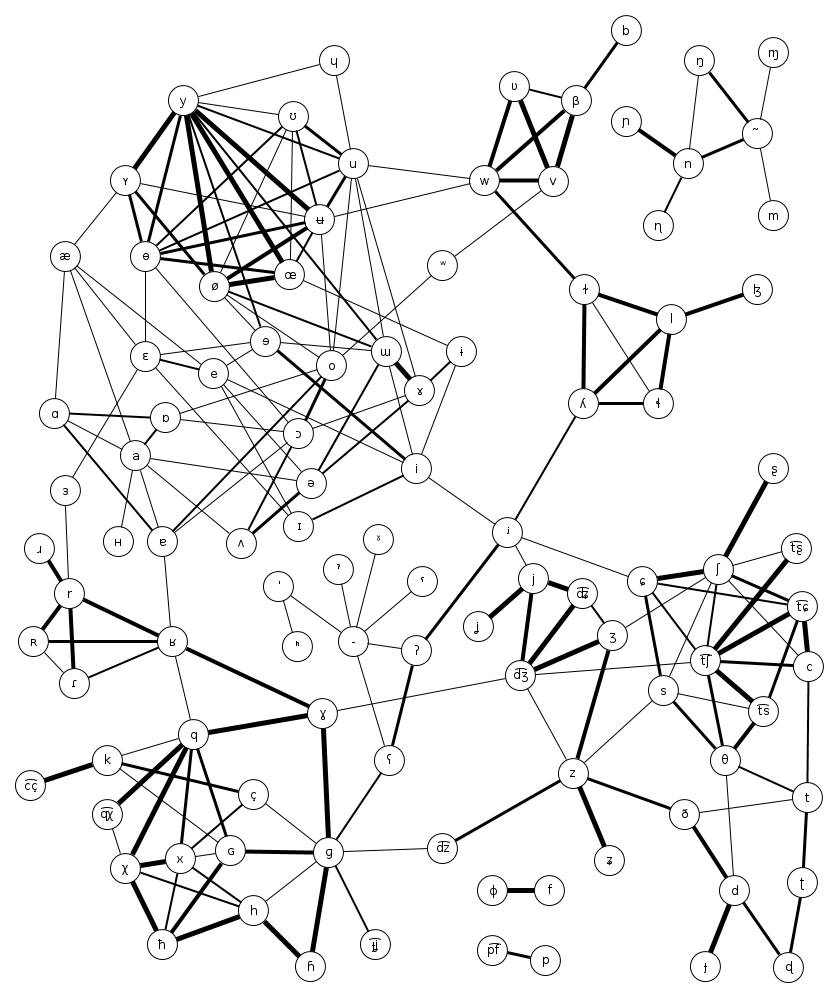
\includegraphics[width=\textwidth]{figures/phoneme-neighbor-graph.png}
    \caption{Visualization of phoneme similarity as inferred from the NorthEuraLex data}
    \label{fig:phonemDistGlobal}
\end{figure}

After iterating the scoring scheme three times in order to include more distant cognates based on rough earlier approximations, the result derived from a final number of more than 300,000 good cognacy candidate pairs in NorthEuraLex is visualized in \figref{fig:phonemDistGlobal}. All segment distance scores lower than 0.5 are visualized as links, and the thickness of the lines represents the similarity of the segments. A perhaps more readable representation of global sound segment correspondences was given in the overview of the IPA inventory already, where the neighbors are sorted by ascending distance, and distances between 0.5 and 0.6 are additionally given in gray color. The asymmetry in some of the neighbor relations is due to the fact that values vary slightly with the random permutations used for estimating $\hat{c}(a,b)$. In tests, this slightly non-deterministic behavior remained even for 100 resamples, and only has negligible effects in later computations.

\subsection{Inferring pairwise correspondences for NorthEuraLex}
To infer sound correspondence models for each pair of languages, we repeat the procedure that we
used for inferring the global sequence similarities on cognate pairs for that language pair.
The core idea is that if strong sound correspondences are found, they will represent the
type of correspondences we can expect in true cognates. Because the local model for unrelated
languages will not find any correspondences beyond random noise (or at least, the signal will
be weaker than the global sequence similarities), we need to maintain the global correspondences
in order to find loanwords between unrelated languages. This motivates the design choice
to define the combined distance $d(s_1,s_2)$ between two segments as the minimum
of the global distance $d_{glo}(s_1,s_2)$ and the local distance $d_{L_1,L_2}(s_1,s_2)$.
In this, the architecture presented here differs significantly from the approach implemented
in LingPy, where the alignment scores are based on a mixture of global and pair-specific
correspondence scores, and not the minimum.

We conclude the discussion of sound correspondence inference by taking a closer look at the inferred correspondences for several language pairs. \figref{fig:driftGraphEnDe} visualizes the inferred correspondences between \ili{English} and \ili{German} in the form of what I will call a \textit{\isi{drift graph}}. Between all the IPA segments present in one language, we visualize all segment distances below a value of 0.5, and use the thickness of lines to represent segment similarity. Global correspondences which were not strengthened by inference of correspondences remain in black, whereas green arrows represent correspondences which were strengthened from the perspective of the first language. The arrows can thus be read as the regular sound changes which would be inferred under the assumption that the first language developed into the second one.

For \ili{English} and \ili{German}, most sound correspondences are inferred correctly. For instance, English \ipa{[p]}, while corresponding to German \ipa{[\t{pf}]} in most contexts, often corresponds to \ipa{[f]} due to subsequent simplification, as can be seen in examples such as the cognate pairs \textit{ripe} and \textit{reif}, \textit{sharp} and \textit{scharf}, and \textit{sheep} and \textit{Schaf}. Also, an apparent chain shift \ipa{[D]} $\rightarrow$ \ipa{[d]} $\rightarrow$ \ipa{[t]} $\rightarrow$ \ipa{[\t{ts}]} becomes very clearly visible. The detected shifts correctly represent the High German consonant shift which occurred in the southern parts of the West Germanic dialect continuum, giving rise to \ili{Old High German}. Other prominent correspondences include \ipa{[s]} $\rightarrow$ \ipa{[z]} (as in \textit{sun} \ipa{[s2n]} vs. \textit{Sonne} \ipa{[zOn@]}), \ipa{[v]} $\rightarrow$ \ipa{[b]} (as in \textit{give} \ipa{[gIv]} vs. \textit{geben} \ipa{[ge:b@n]}), and \ipa{[w]} $\rightarrow$ \ipa{[v]} 
(as in \textit{water} \ipa{[wO:t@]} vs. \textit{Wasser} \ipa{[vas5]}).

\begin{figure}
    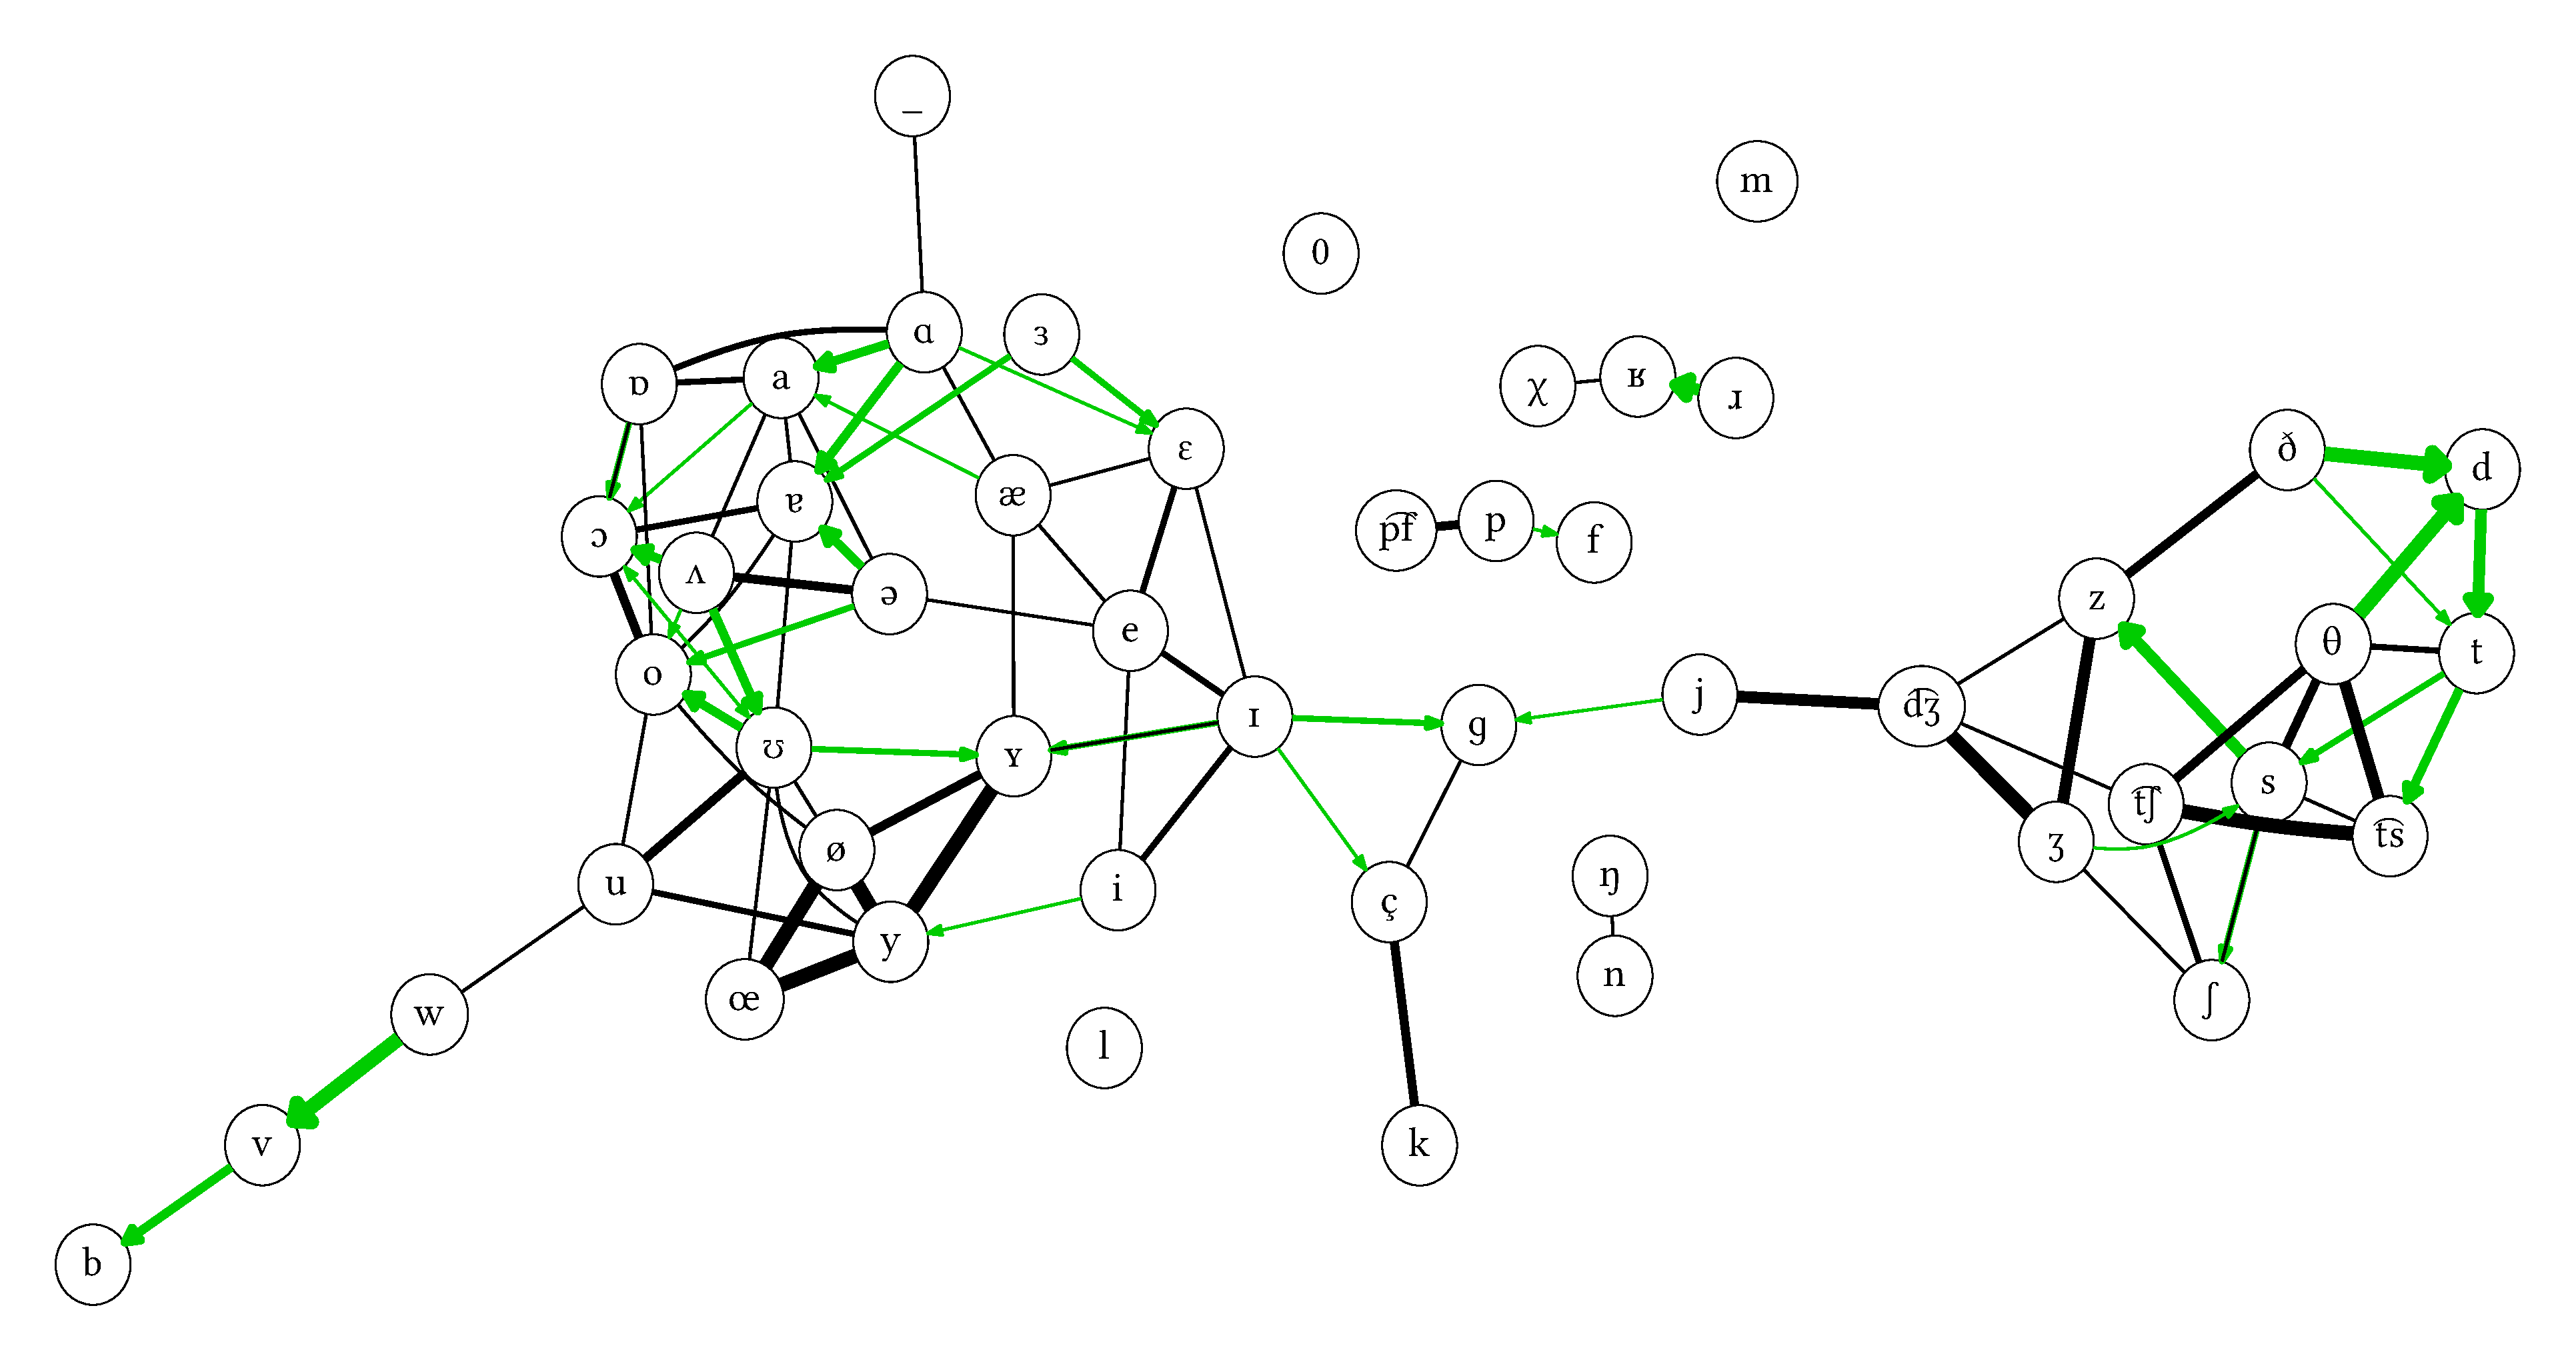
\includegraphics[width=\textwidth]{figures/drift-graph-en-de.pdf}
    \caption{Drift graph of inferred correspondences from English to German}
    \label{fig:driftGraphEnDe}
\end{figure}

Turning to another pair of closely related Indo-European languages, we take a look at the drift graph from \ili{Lithuanian} to \ili{Latvian} in \figref{fig:driftGraphLtLv}. Here, we have some very prominent correspondences without which an automated system would fail to find many cognates even between this closely related pair of languages. The three most prominent correspondences are Lithuanian \ipa{[k]} and Latvian \ipa{[\t{ts}]}, (reflected in cognate pairs such as \textit{kepti/cept} `to bake' and \textit{lokys/l\={a}cis} `bear'), Lithuanian \ipa{[g]} vs. Latvian \ipa{[\t{dz}]} (as in \textit{giesm\.{e}/dziesma} `song' or \textit{gyventi/dz\=ivot} `to live'), and Lithuanian \ipa{[V]} vs. Latvian \ipa{[f]} (due to devoicing in Latvian in pairs such as \textit{t\.{e}vas/t\={e}vs} `father' or \textit{\v{z}uvis/zivs} `fish'). There is a problematic (though weak) correspondence between \ipa{[n]} and \ipa{[O]}. Inspection of the alignments shows that this happens in cognates where Lithuanian \textit{an} \ipa{[5n]} corresponds to Latvian \textit{o} \ipa{[uO]} (also reflecting ancestral \textit{*an}) in word pairs such as \textit{ranka/roka} `hand' and \textit{antras/otrais} `second', which cannot be modeled by single-segment correspondences.

\begin{figure}
    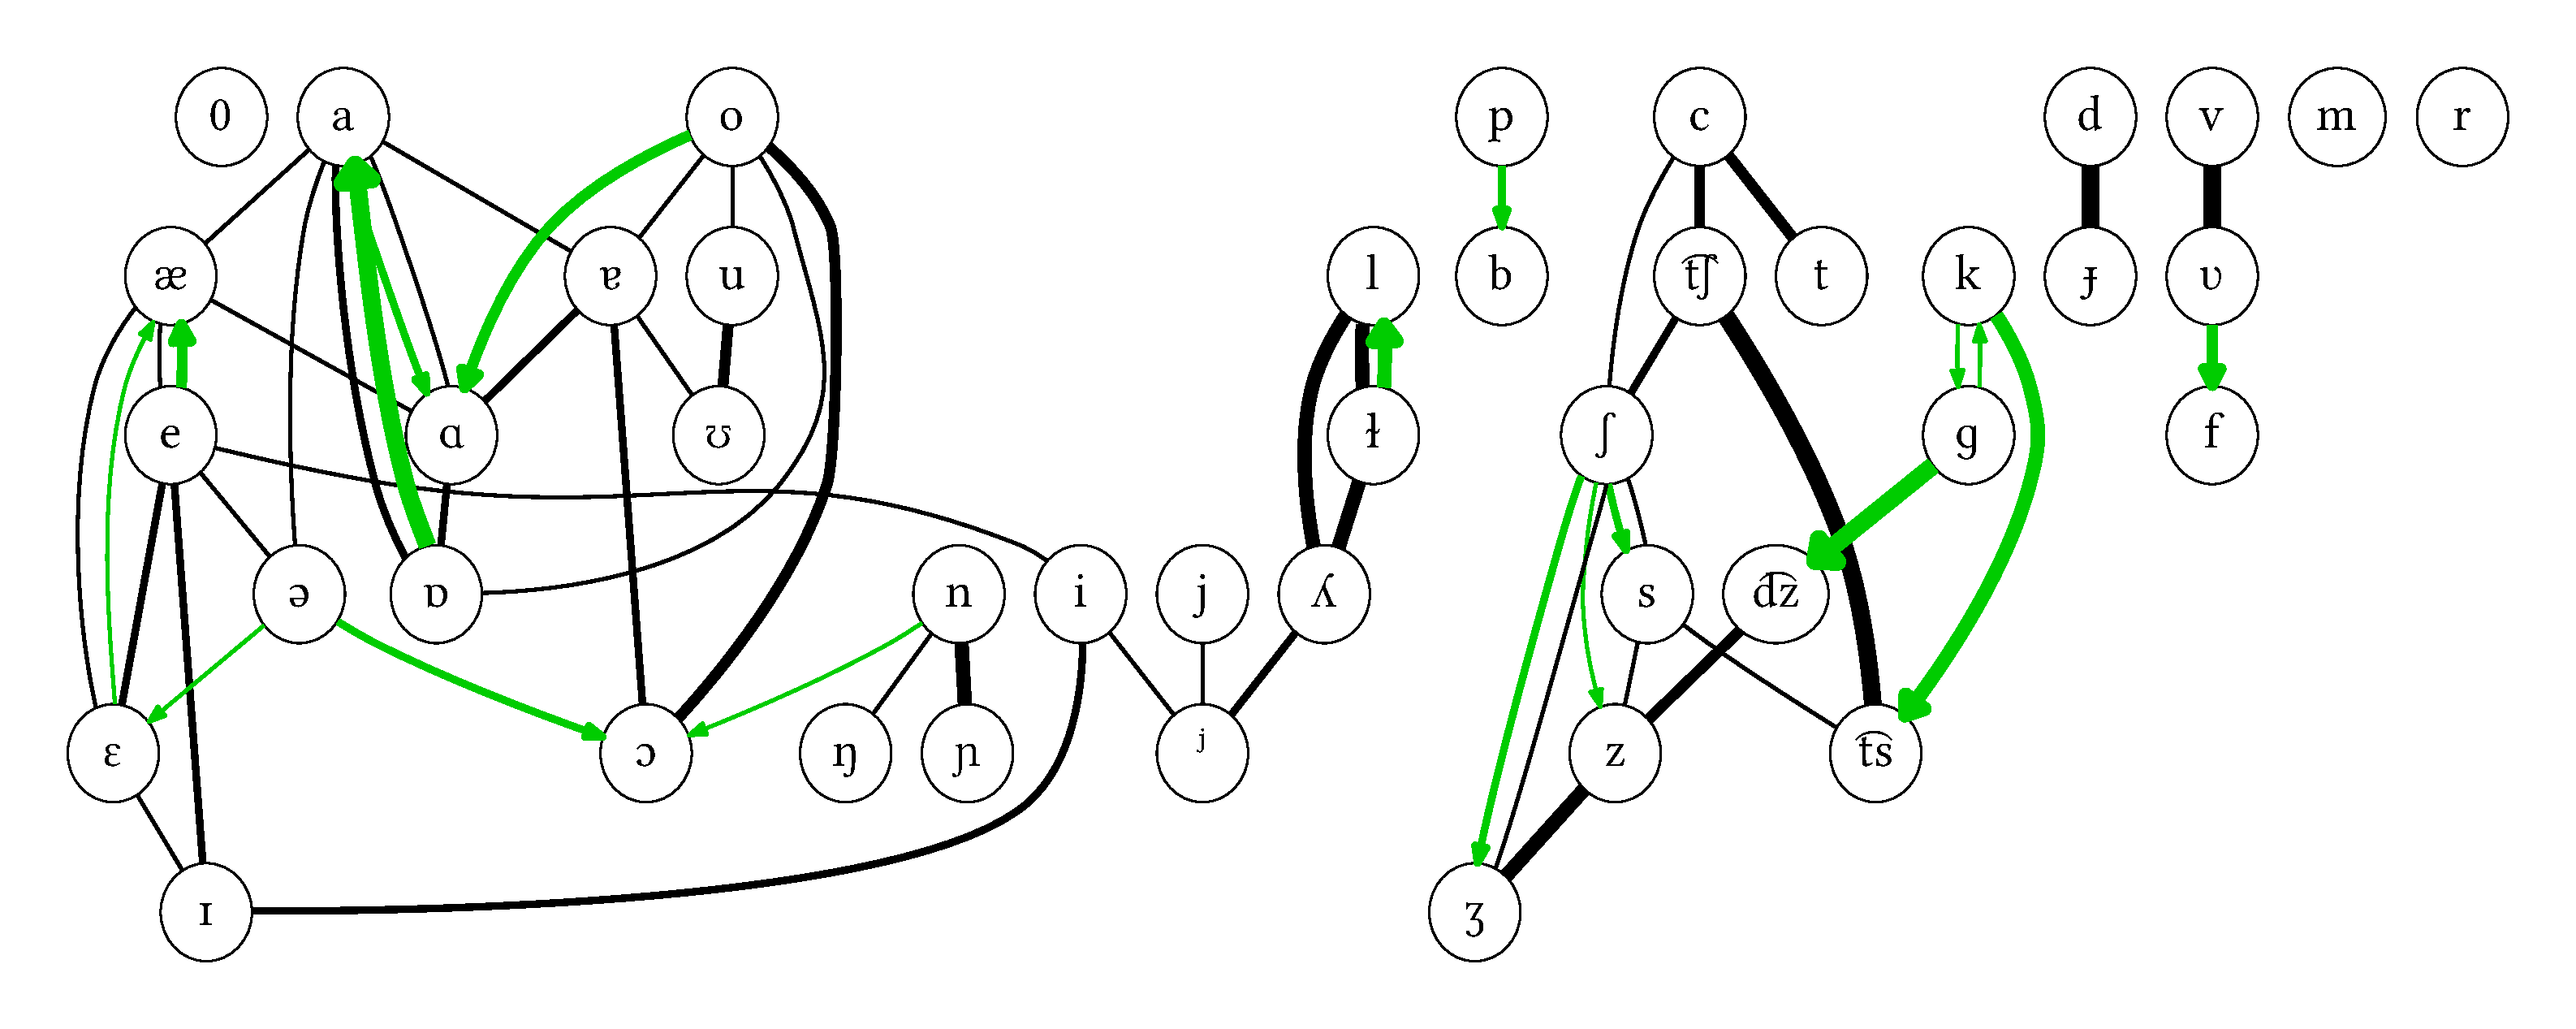
\includegraphics[width=\textwidth]{figures/drift-graph-lt-lv.pdf}
    \caption{Drift graph of inferred correspondences from Lithuanian to Latvian}
    \label{fig:driftGraphLtLv}
\end{figure}

Moving to a second language family, we inspect the drift graph from \ili{Finnish} to \ili{Northern Saami} in \figref{fig:driftGraphFiSe}. While some of the inferred shifts make a lot of sense, we quickly notice that some of the inferred correspondences are a lot less plausible than the examples we have seen so far. For instance, there are weak correspondences \ipa{[E]}/\ipa{[S]} and \ipa{[n]}/\ipa{[c]} which seem completely out of place. Inspection of the relevant alignment pairs shows that much like in the case of the erroneous correspondence between Lithuanian and Latvian, these patterns are due to non-root segments. Some Finnish nouns in \textit{-e} which historically ended in \textit{*-ek} are cognate with Northern Saami nouns in \textit{-a\v{s}}. Examples in the NorthEuraLex database include \textit{murhe/mora\v{s}} `sorrow', \textit{perhe/beara\v{s}} `family', and \textit{k\"a\"arme/gearpma\v{s}} `snake'. The reasons for the erroneous inference of \ipa{[n]}/\ipa{[c]} are more subtle. Relevant pairs 
include \textit{sanoa/dadjat} `to say' and \textit{huono/headju} `bad'. In both of these cases, Saami \textit{dj} \ipa{[cc]} overlaps in alignments with Finnish \textit{n}, a situation which occurs too often to be attributable to chance, and is therefore resolved by matching the Finnish \ipa{[n]} with one of the \ipa{[c]} sounds of the Saami geminate.

\begin{figure}
    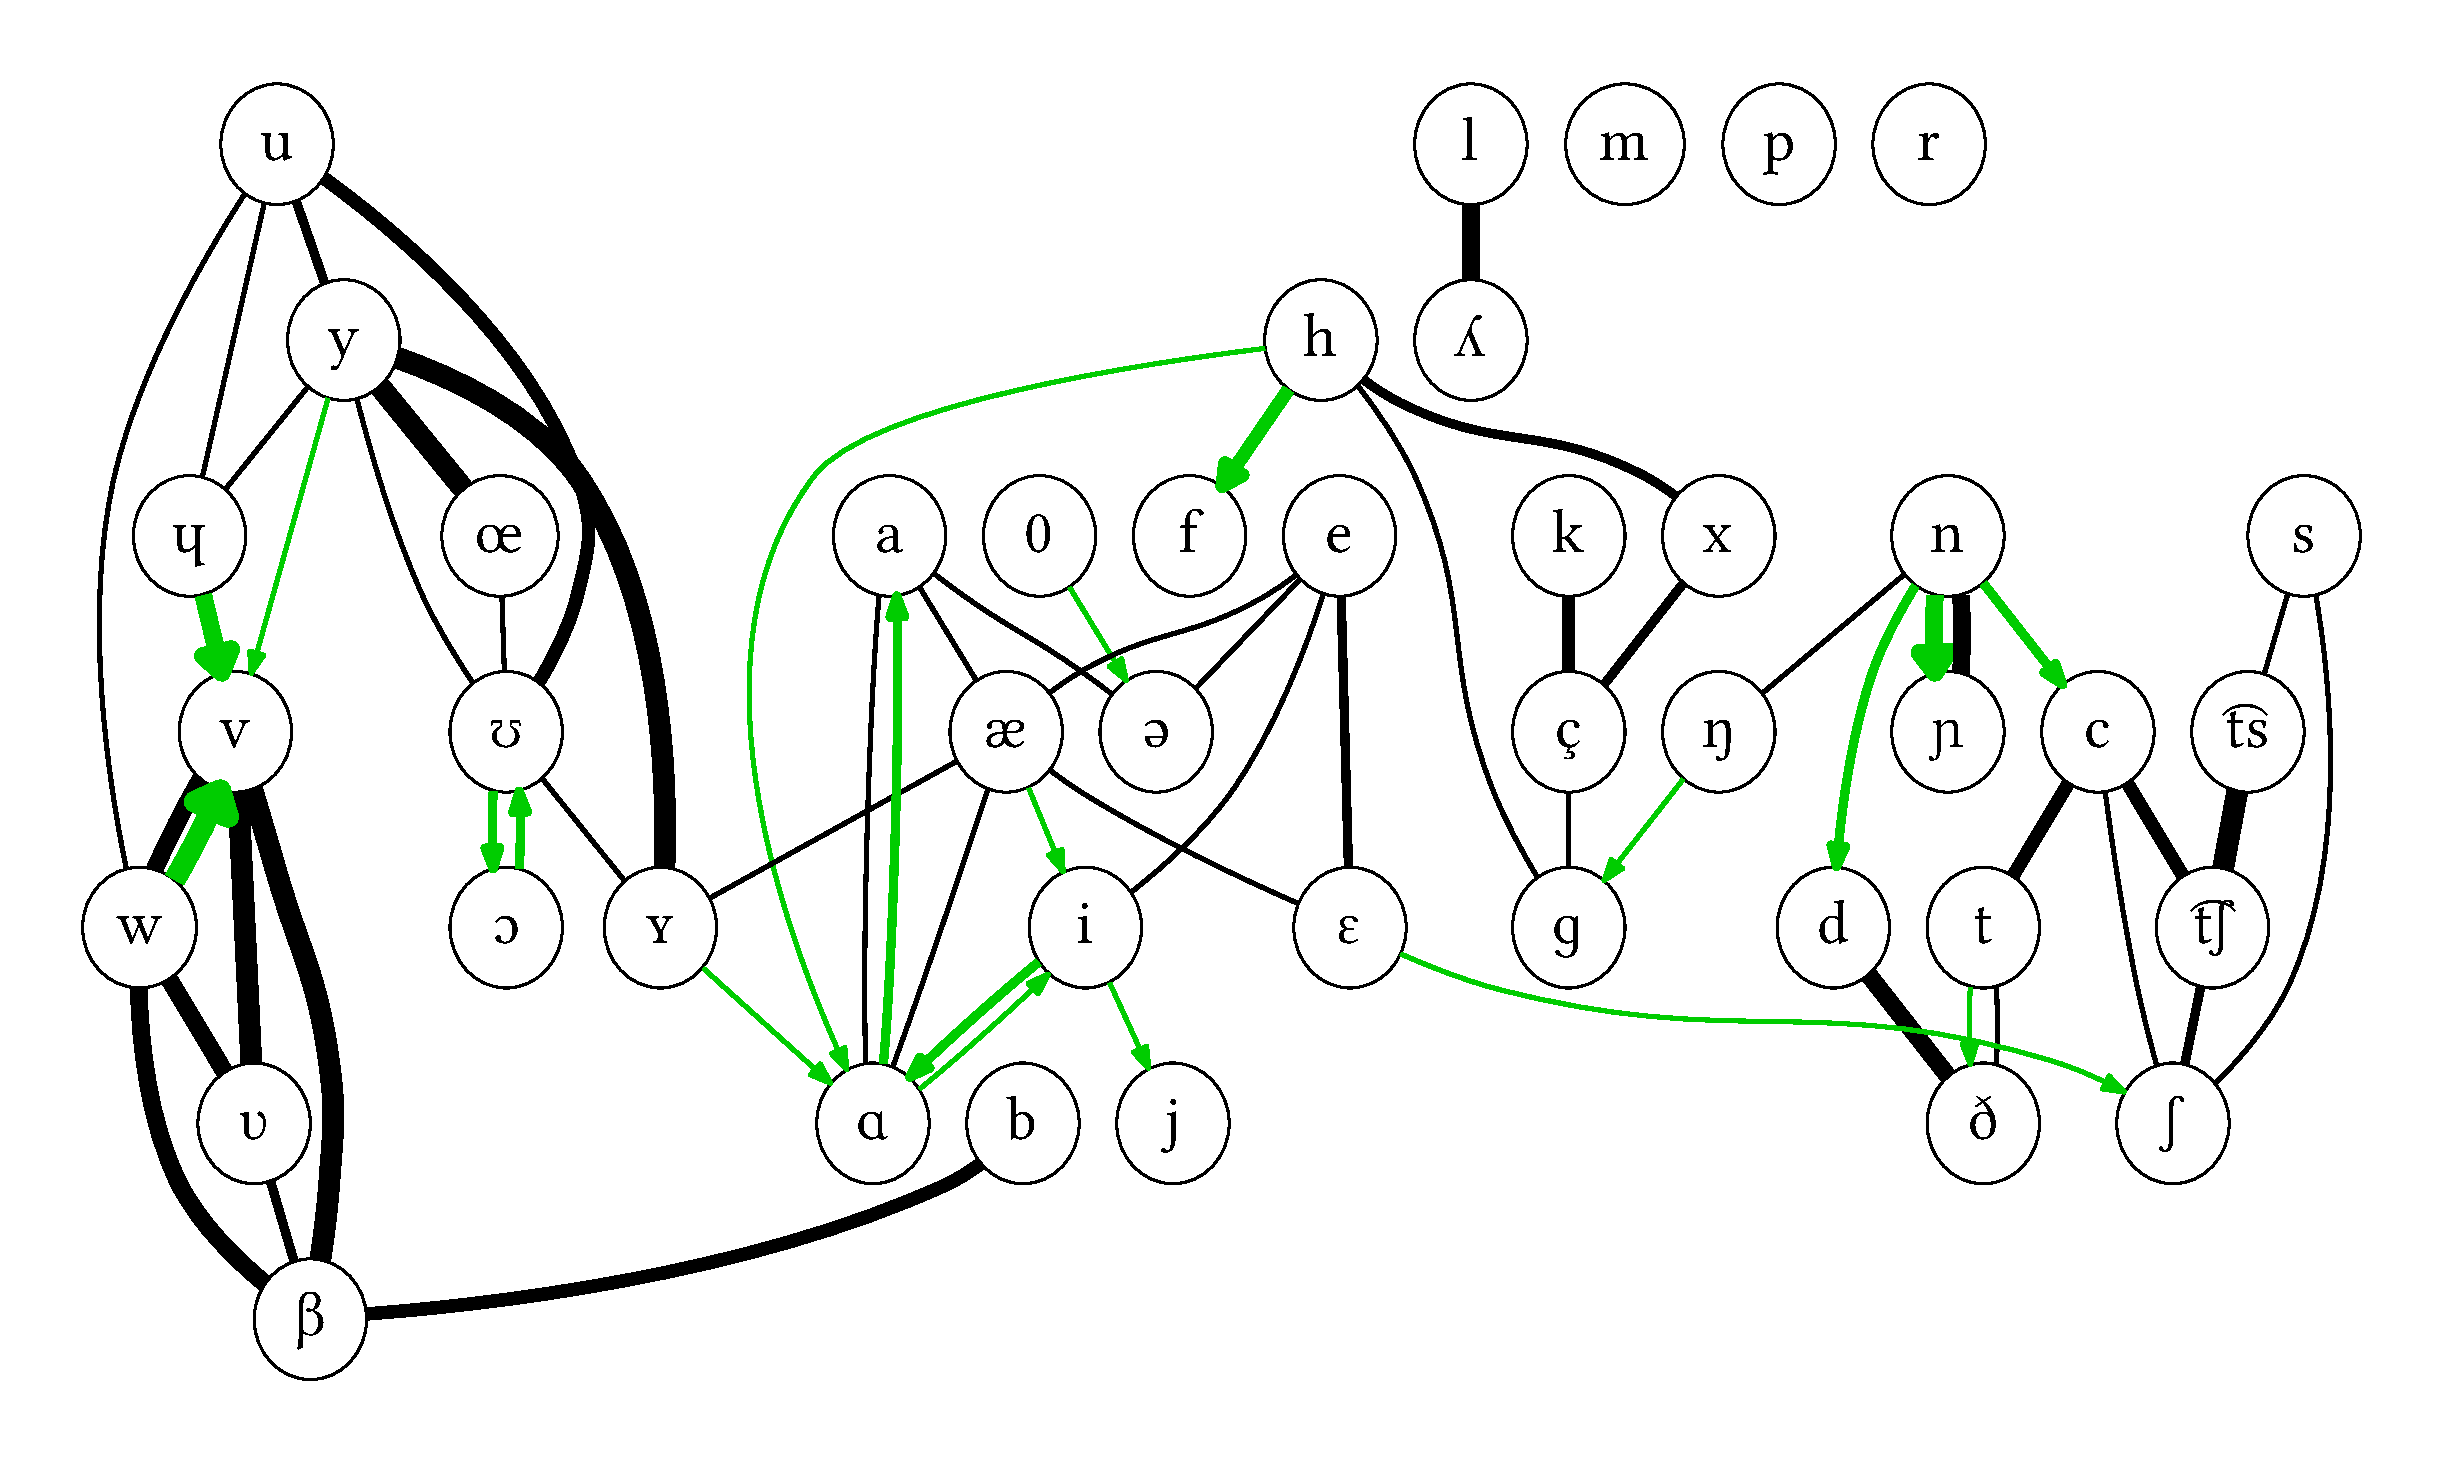
\includegraphics[width=\textwidth]{figures/drift-graph-fi-se.pdf}
    \caption{Drift graph of inferred correspondences from Finnish to Northern Saami}
    \label{fig:driftGraphFiSe}
\end{figure}

Much more difficult to recognize, due to the low number of cognates, are the major sound shifts which separate \ili{Finnish} from \ili{Hungarian}. The relevant drift graph in \figref{fig:driftGraphFiHu}, however, still clearly shows two of the major sound shifts which occurred in the history of Hungarian. The correspondence \ipa{[k]}/\ipa{[h]} is correctly inferred from cognate pairs such as \textit{kala/hal} `fish' and \textit{kuulla/hall} `to hear', and the correspondence \ipa{[p]}/\ipa{[f]} covers pairs such as \textit{puu/fa} `tree' and \textit{p\"a\"a/f\H{o}} `head'. The vowel correspondences are a lot more chaotic, and also less well-represented, leading to fewer local correspondences among vowels, except a tendency to map Finnish \textit{e} \ipa{[E]} to Hungarian \textit{\'e} \ipa{[e]}, due to cognate pairs such as \textit{pes\"a/f\'eszek} `nest', and a mapping of the vowel \ipa{[u]} (much more frequent in Finnish than Hungarian) to \ipa{[6]}, which is very frequent in Hungarian, but does not occur 
in Finnish. The mapping of Finnish \textit{\"a} \ipa{[\ae]} to the gap symbol is mainly due to the fact that an overwhelming majority of dictionary forms of Finnish words ends in a vowel, whereas Hungarian has undergone a process of monosyllabification (as evidenced in some of the examples above). The purpose of the cheap vowel-to-gap mappings for modeling Finnish-Hungarian cognates is therefore to reduce the costs of deleting the trailing vowel from the Finnish lexemes, which contains little information that would be relevant for comparison with Hungarian.

\begin{figure}
    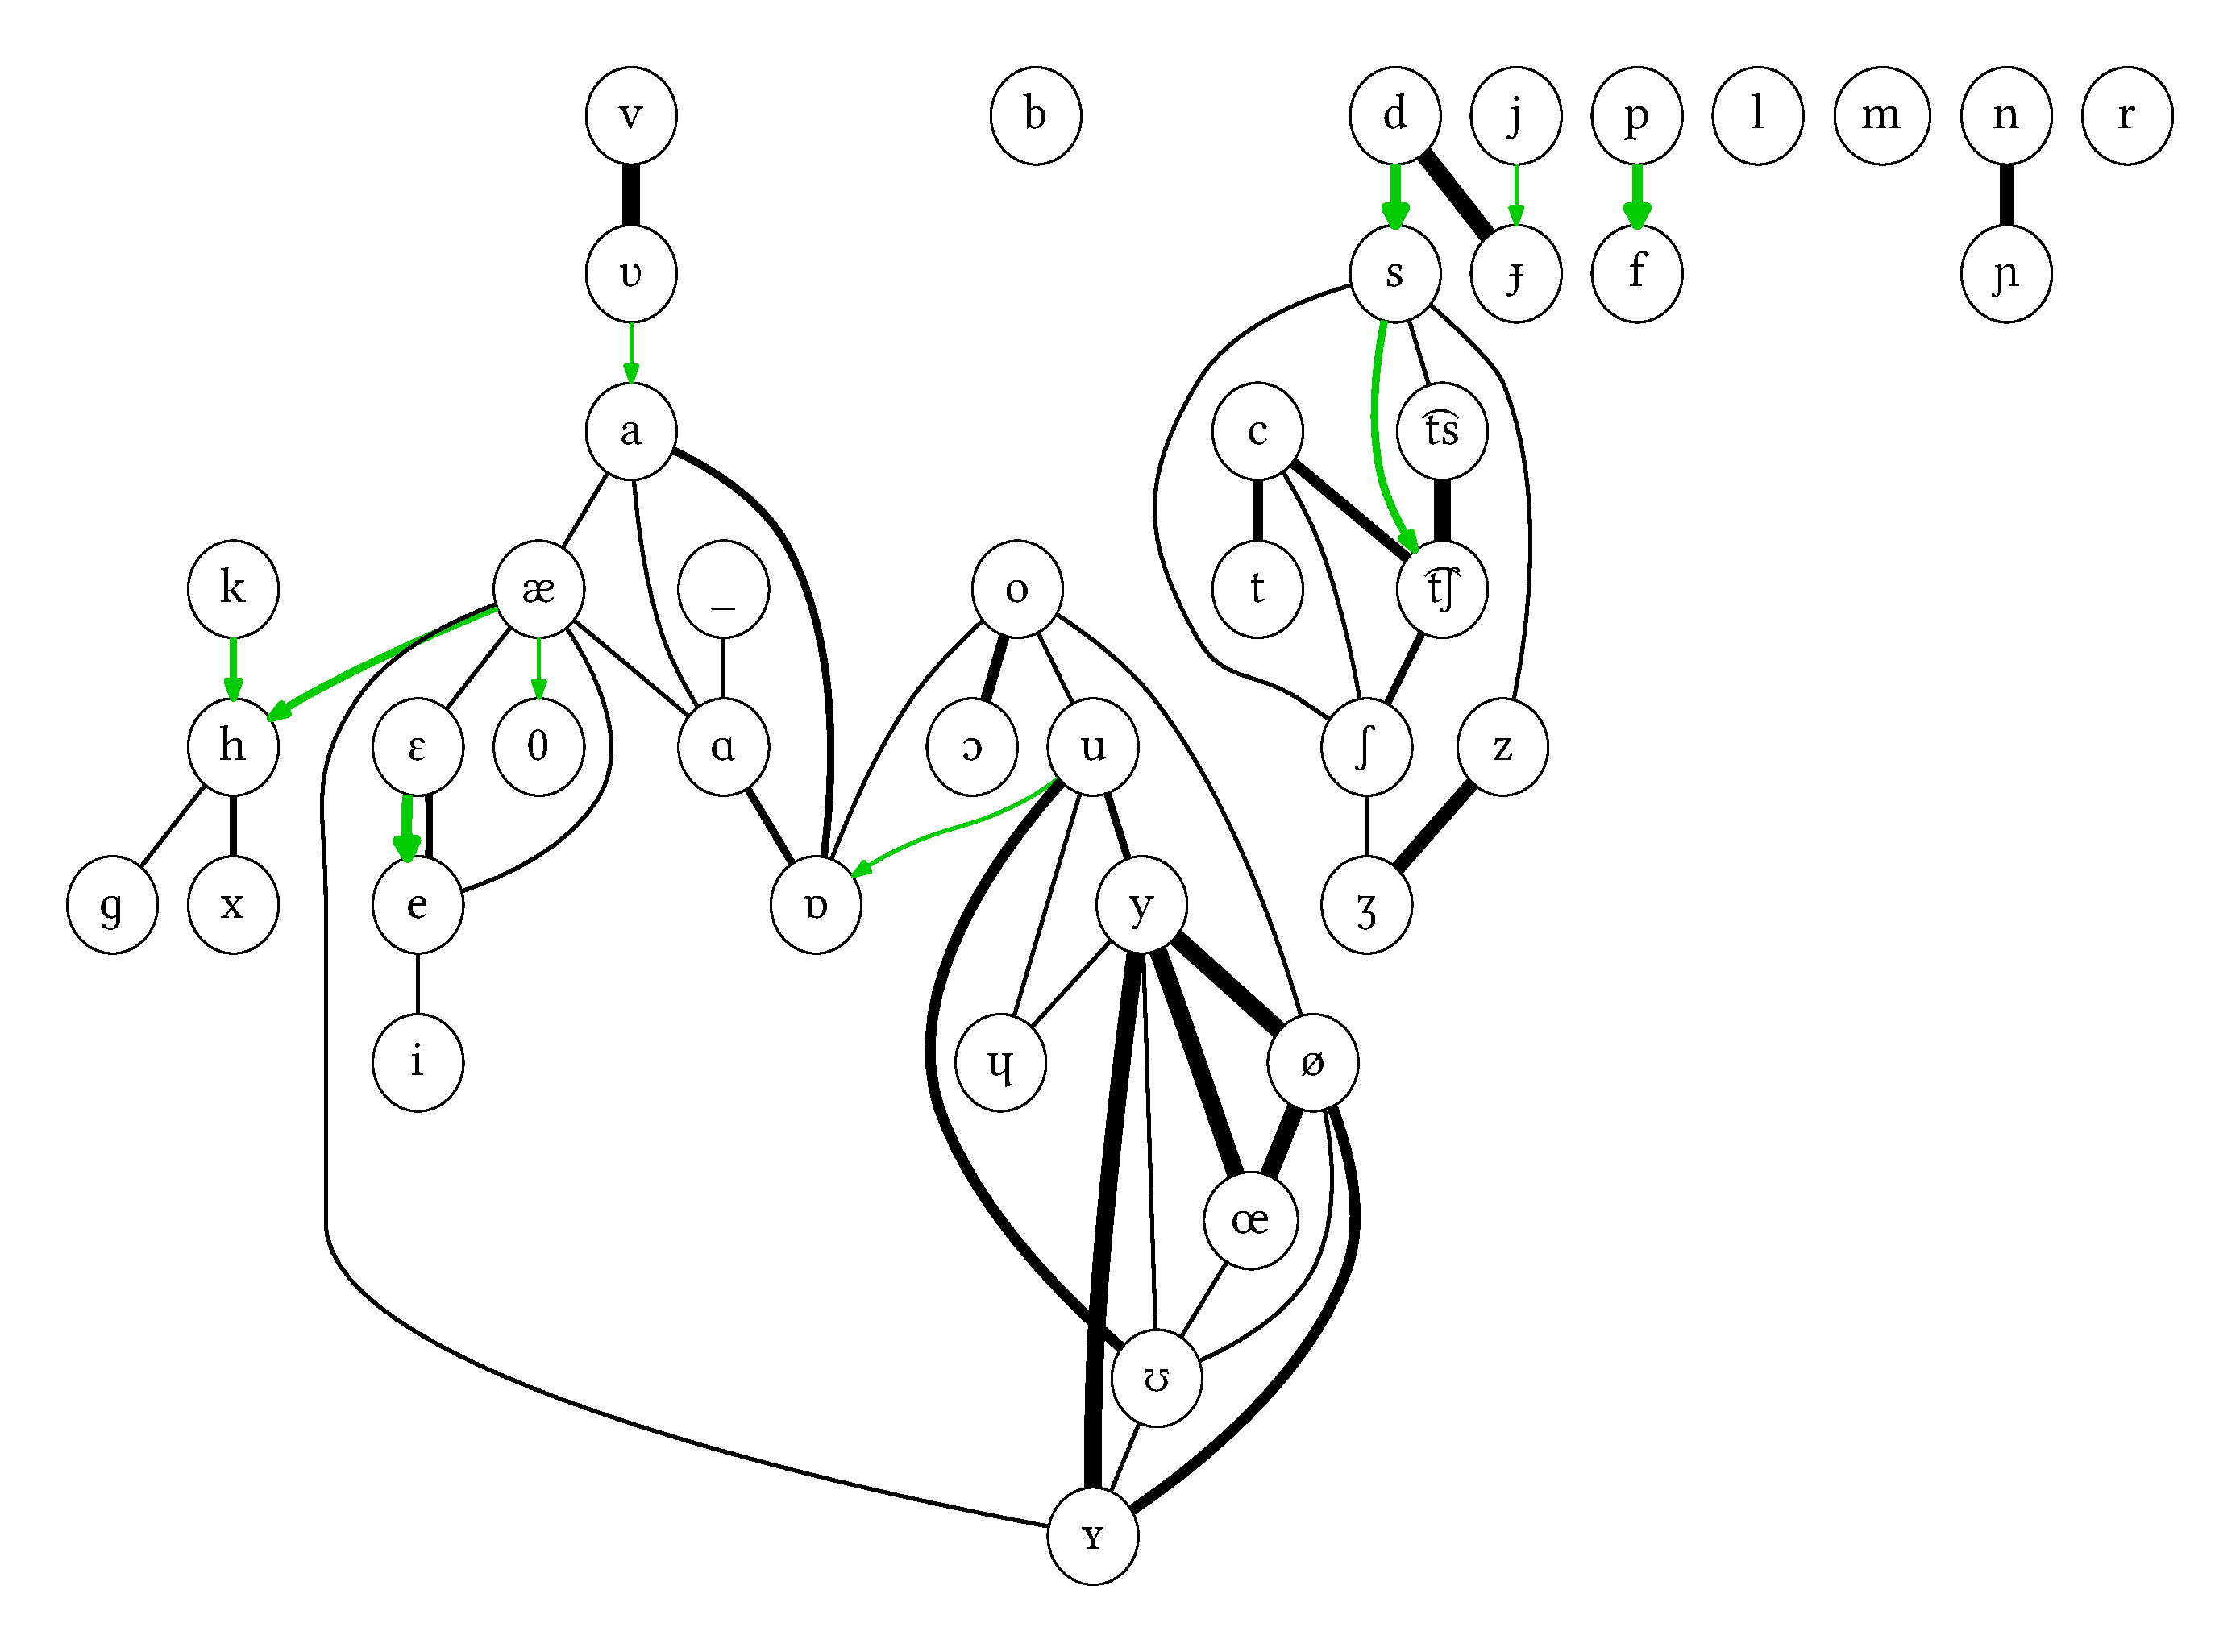
\includegraphics[width=\textwidth]{figures/drift-graph-fi-hu.pdf}
    \caption{Drift graph of inferred correspondences from Finnish to Hungarian}
    \label{fig:driftGraphFiHu}
\end{figure}

Finally, to illustrate that no local sound correspondences are inferred for a typical pair of unrelated languages, the drift graph from \ili{Basque} to \ili{Nivkh} is given in \figref{fig:driftGraphEuNiv}. As expected, we see almost no green arrows in this drift graph, and the two arrows which do exist are very thin, indicating only small changes to the phoneme distances. Here, the spurious correspondence \ipa{[i]}/\ipa{[c]} is due to the fact that a large class of Basque verbs ends in \textit{-i}, whereas the dictionary form of the Nivkh verb virtually always ends in \textit{-t'}, which is pronounced \ipa{[c]}. Without information weighting detecting and modeling that these elements are not very informative, the effect of this systematic pattern would have been much stronger. The \ipa{[s]}/\ipa{[h]} correspondence is due to the low frequency of word-initial \ipa{[h]} in Nivkh and the high frequency of \ipa{[s]} (written \textit{z}) in Basque, combined with a handful of spurious similarities such as \textit{azal} and \textit{hal} `skin'.

\begin{figure}
    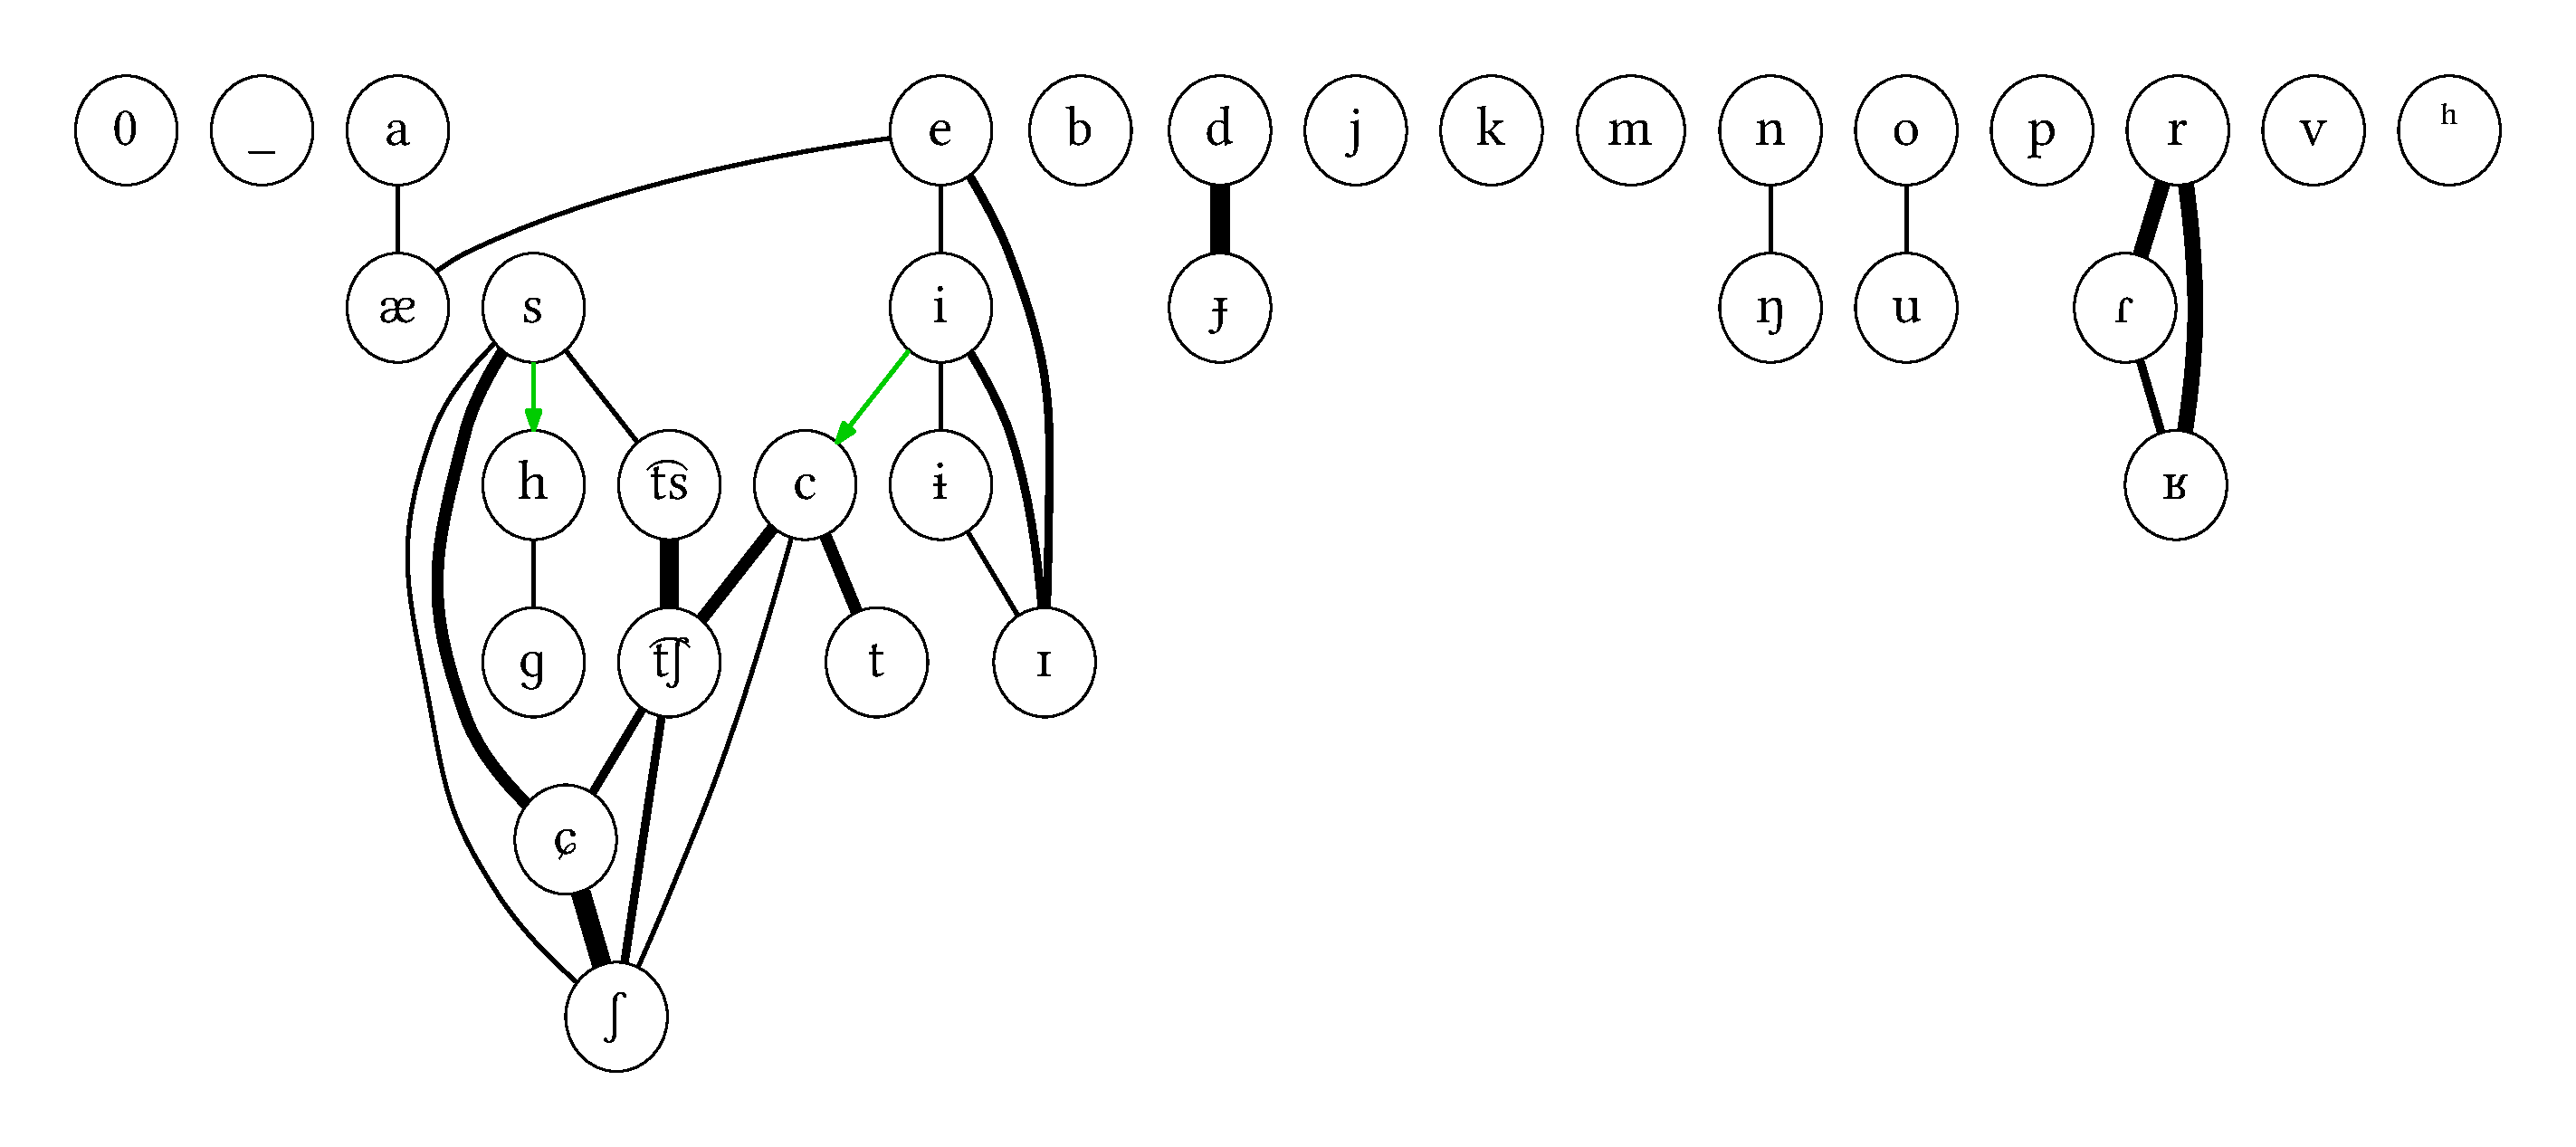
\includegraphics[width=\textwidth]{figures/drift-graph-eu-niv.pdf}
    \caption{Drift graph of inferred correspondences from Basque to Nivkh}
    \label{fig:driftGraphEuNiv}
\end{figure}

\subsection{Aligning NorthEuraLex and deriving form distances}

Unlike the LexStat sequence distance by \cite{list2012}, IWSA does not need to be modified by using an end-space free variant of the dynamic programming algorithm, because recurrent prefixes and suffixes are treated by the information weighting, and compounds must not be treated as full cognates. For a recent treatment of partial cognacy, the case I am avoiding, the reader is referred to recent work on detecting partial cognacy by \cite{list_ea_2016}.

The main building block of my procedure for deriving form distances from NorthEuraLex is thus IWSA on word class-specific information models, combined with a scoring scheme which maps both global and pair-specific phoneme distance scores onto $[0,1]$ by cutting off extreme values of mutual information.

\section{Cognate clustering}\label{sec:4.5}
The final step in the pipeline from raw phoneme sequence data to an estimate of cognate sets is to derive cognate sets from the normalized sequence distances. For this step, I will not attempt to introduce any new ideas. Instead, this section gives an overview of current approaches to the cognate clustering problem, and motivates the use of a comparatively well-established method for the purposes of my research.

\subsection{The cognate detection problem}
The binary cognacy judgments problem can be simplified considerably by exploiting the fact that cognacy judgments should be transitive, i.e.\ if we assume a pair of words $w_1$ and $w_2$ to be cognates, and a third word $w_3$ to be cognate with $w_2$, we must also assume that $w_1$ and $w_3$ are cognates. Mathematically, this reduces a solution to the cognate detection problem to a partition $W = W_1 \uplus W_2 \uplus \dots \uplus W_n$ of a set of phonetic strings $W$, such that $w_i$ and $w_j$ represent words with a common ancestor iff $w_i,w_j \in W_k$ for one of the sets $W_k$. From an algorithmic perspective, deriving such a partition is a clustering problem, for which well-defined solutions exist if there is a distance matrix which defines the dissimilarity between each pair of data points. This is the approach taken by practical solutions to cognate clustering, at least as a final step.

\subsection{Approaches to cognate clustering}
A very quick and simple method for cognate detection was proposed by \cite{turchin_ea_2010}, who reduce the phonetic forms to nine consonant classes of roughly the same granularity as the Dolgopolsky classes, and approximate cognacy judgments by defining two words to be cognate iff the first two consonant classes are identical. The binary judgments are not explicitly used to create cognate sets, because the authors are only interested in statistical evidence of language-wide long-distance relationships. Still, a definition based on identity is trivially transitive, turning this into a very quick and at least partially linguistically motivated way of partitioning a list of phoneme sequences into rough cognate classes.

We now come to the more mainstream approaches, where some distance matrix between surface forms is given. On data of this type, a wide range of well-understood clustering algorithms can in principle be used to derive cognate sets. Popular algorithms include hierarchical (i.e.\ tree-building) clustering algorithms such as single-linkage clustering, complete linkage clustering, and UPGMA \citep{sokal_michener_1958}. Centroid-based clustering algorithms such as k-means clustering \citep{lloyd1982} are only of very limited use to this application, because we do not have an explicit feature representation of the objects (put differently, the objects are not explicitly represented as vectors in a space). While kernelized variants of some clustering algorithms could in principle be used, the usage of clustering algorithms which operate on the level of single links is much more natural on data which comes in the shape of a distance matrix.

Hierarchical clustering algorithms are the most obvious choice for a task where we have nothing more than distance values for all pairs of objects. For instance, UPGMA derives a hierarchical clustering (a tree) over the data points by iteratively adjoining the element that has the smallest average distance to one of the existent clusters (= subtrees) as a sister node to the head of that subtree. To derive a partition into cognate sets from such a hierarchical clustering, all one needs to do is to stop the process at a user-defined threshold value before the entire tree is constructed, and to treat the subtrees created so far as cognate sets. Since the output of this variant does not include a tree structure, it is called flat UPGMA.

The disadvantage of any hierarchical clustering method is that it is difficult to avoid chaining effects, where very distant points are erroneously clustered together through a dense chain of intermediate points which build a bridge between the two distant points. Since no alternative clustering paradigm is without such weaknesses, UPGMA remains the default method for deriving cognate clusters from form distance matrices. For instance, the cognate clustering in LingPy is implemented by running UPGMA up to a user-defined threshold on user-definable form distances, the default being the distances inferred by LexStat or SCA.

Moving beyond UPGMA, attractive alternative clustering algorithms for the cognate detection task have recently been found in the community detection literature. Community detection algorithms can be applied to cognacy detection by creating a node for each word form, and connecting all pairs of forms below a certain distance threshold. In the algorithms which operate on weighted networks, the weights of the connections can be defined from the form distances. The communities found in the network, subgraphs which are in some sense more strongly connected internally than to other parts of the graph, can then be interpreted as representing cognate clusters.

Among community detection algorithms, label propagation\is{label propagation algorithm} by \cite{raghavan_ea_2007} is conceptually the most simple, and it is also very efficient because it is based on local update decisions. The core procedure of the unweighted variant is to start with a unique label on each node, and then to iteratively reassign the labels, letting each node adopt the label shared by most of its neighbors. In situations where there is no single such label, the new label is selected through uniform sampling among the best options. The process is stopped once every node has at least as many neighbors with its current label as with any other label. As the authors show, nodes with identical labels agree very well with the community structure in several interesting types of networks. While label propagation has the advantage of avoiding chaining effects, it has a problematic tendency to assign every node to one of the larger clusters, leading to quite a few false positives if some words do not 
have any cognate in the input set.

The InfoMap community detection algorithm\is{InfoMap algorithm} by \cite{rosvall_bergstrom_2008} tends to perform better in this respect, and has therefore gained some traction in the field as a useful alternative to UPGMA. InfoMap is based on sampling random walks through the network to derive a representation of information flow. Concepts of information theory are used to map partitions into two-level encodings for random walks, where efficient encodings lead to shorter descriptions of the random walks. Using general optimization techniques to derive a partition whose two-level encoding minimizes the expected description length of a random walk, the algorithm infers a macro-structure which compactly represents the network, and can be interpreted to reveal the community structure.

Very recently, \cite{list_ea_2017} compared the performance of Turchin's criterion as well as UPGMA on edit distance, UPGMA on SCA distance, UPGMA on LexStat distance, and InfoMap on LexStat distance, on a reasonably wide range of single-family datasets contributed by experts. Surprisingly, they find that the accuracy across all the approaches only varied between 82\% and 89\%, with LexStat performing best, and a very slight advantage for InfoMap clustering over UPGMA. \cite{rama_ea_2017} combine PMI-based distance scores with InfoMap clustering, and evaluate the resulting system on a range of datasets against LexStat, as well as an alternative distance score derived from Pair Hidden Markov Models (PHMM). On a range of test sets, they find that PMI scores trained in an unsupervised fashion using online expectation-maximization, in combination with the Needleman-Wunsch algorithm and InfoMap clustering, beat LexStat by a small margin on a number of datasets. On average, both LexStat and their best system are 
again not much better than normalized Levenshtein distance (0.819/0.842 vs. 0.804) in the B-Cubed F-score measure used by both papers to measure accuracy. It therefore seems relatively easy to achieve a quite respectable performance using any method, while improving on the already good baseline performance of simple methods appears to be quite difficult. From the perspective of a historical linguist, it is at least promising to see that the correspondence-based LexStat distances and PMI-based distances come out on top across approaches and datasets.

Within the machine learning paradigm, cognate detection can alternatively be viewed as a binary classification problem. This implies using test data to let a system learn to make correct binary decisions (cognate or non-cognate) for pairs of words. Early work in this direction is summarized by \cite{rama2015}, who trains a Support Vector Machine (SVM, a mainstream model in machine learning) over a feature representation that encodes shared subsequences, and shows that this feature set outperforms earlier SVM-based attempts. Moving to non-linear classifiers, \cite{rama2016} applies a convolutional neural network (CNN) on handcrafted representations of ASJP data, and shows that this approach is quite successful at deciding cognacy between pairs of words from smaller families. Unfortunately, the results are not compared to other approaches outside the binary classification paradigm.

Since the results of pair-wise classification will typically not lead to a consistent result (as the cognacy relation is transitive, whereas binary decisions taken in isolation will typically not be), it will typically need to be combined with an additional clustering stage in order to arrive at a partition into cognate sets. This is the approach taken by \cite{jaeger_sofroniev_2016}, who train an SVM to predict pairwise probabilities of non-cognacy from phonetic distances, overall language distance, and average word length, and combine the result with UPGMA clustering to derive the cognate sets. The method is reported to slightly outperform LingPy's LexStat method on the cognate clustering task, and seems to profit from better clustering methods. Given sufficient amounts of training data, supervised machine learning methods for classification have thus started to show some promising results for the cognate detection task.

Unfortunately, the way in which all these methods have so far been evaluated does not tell us much about their performance on a dataset like NorthEuraLex which spans several language families. For such multi-family datasets, it makes sense for a system to put more effort into avoiding false positives, whereas for intra-family comparison, the probability that two similar-looking words for the same concept are not cognate is very small. Since we do not yet have a cognacy-annotated subset of NorthEuraLex which spans several language families, supervised machine-learning methods are impossible to apply. Still, comparing my own IWSA-based system to LingPy provides some indication of how it would fare against these methods, given that they have so far not managed to outperform LingPy significantly.

\subsection{Deriving cognate sets from NorthEuraLex}
By using the same variant of the UPGMA algorithm as LingPy, I am opting for a well-established method for deriving cognate sets inference from form distances. To derive the threshold value for my IWSA-based distances, manual inspection of the cognate sets for a handful of concepts on different threshold values suggested 0.45 as leading to results which best fitted my knowledge about the true cognate sets in Indo-European and Uralic. Since a part of the evaluation we are going to see in the next section is threshold-independent, the empirically determined thresholds from this step will be combined with this impression to decide on the threshold value used for the cognate clustering that the following chapters will build on.

\subsection{Evaluation on IELex intra-family cognacy judgments}
As previously mentioned, the lack of fully cognacy-annotated cross-family data sets makes it difficult to quantitatively evaluate the quality of the cognacy judgments produced by my architecture. Still, it is necessary to at least test on a small subset whether the results are measurably better than the LingPy output, just as the initial inspection in the last section suggested. Also, this small subset can help us in deriving good threshold values if we systematically analyse the precision-recall tradeoff provided by threshold selection.

For this purpose, I was able to use a dataset kindly provided by Pavel Sofroniev, who created the intersection of IELex with an earlier version of the NorthEuraLex database. For the languages and concepts which are covered by both databases, the referenced word forms were manually compared and mapped to each other, producing a database of NorthEuraLex IPA strings with the cognacy annotations given in IELex. After being updated to reflect version 0.9 of NorthEuraLex, the dataset now covers 6,106 words for 185 concepts across 37 Indo-European languages, providing a very interesting test set for cognate detection that is available as part of the supplementary material for this book (see Appendix C).

To derive the LexStat distances and cognacy judgments, I converted the entire NorthEuraLex database into the tabular input format required by LingPy, doing some trivial symbol replacements until LingPy found the input to be free of errors, and running the LexStat method on the entire database, building on code by Johannes Wahle for deriving cognate sets from the ASJP-encoded version of NorthEuraLex. In this code, LingPy is called according to recommendations by Mattis List, which included setting LexStat's threshold parameter to 0.7, and letting the scorer run without preprocessing, but with many iterations. Setting the \texttt{runs} parameter to a rather large number of 1,500 yielded stable results which barely changed when adding additional iterations, and had the advantage of still being able to infer cognate sets from NorthEuraLex in under six hours on an average office machine.

The cognate sets produced by my architecture and by LingPy were then reduced by ignoring all forms which were not in the test set, and throwing away all cognate sets which contained no form from the test set. The resulting cognate sets were converted into 100,155 pairwise cognacy judgments, on which it is easy to define pairwise performance measures like precision and recall. Each pair of words which are cognate according to IELex is counted as a true positive (TP) if it ends up in the same automatically derived cognate set, and as a false negative (FN) if it is not. Assuming the cognacy judgments in IELex to be complete, any pair of words which are inferred to belong to the same cognate set, but assigned to different cognate set IDs in IELex, is counted as a false positive (FP), and any pair that is not cognate in IELex, and is also assigned to two different cognate sets by an automated system, counts as a true negative (TN).

For evaluation, we compare the performance of three form distances in terms of average pairwise precision, and select optimal threshold values for each distance by means of the precision-recall curve. The three distances we are going to infer are LexStat distances to represent the state of the art, and the mixed scores with constant information (WED) as well as with information weighting (IWD) as computed by my implementation, to measure possible improvements due to my way of inferring sound correspondences, and further improvements due to information weighting. \figref{precision-recall-curves} shows the precision-recall curves for all three distances, which visualizes the behavior of the tradeoff between precision and recall under changing threshold values. In the low-recall range (i.e. for the easy cases), LexStat is better than the other two methods, but its precision decays more quickly with higher recall. This makes IWD and WED better suited for the more difficult instances. The fact that the IWD curve is always higher than the WED curve shows the global advantage of information weighting for separating cognates from non-cognates.

\begin{figure}[ht]
 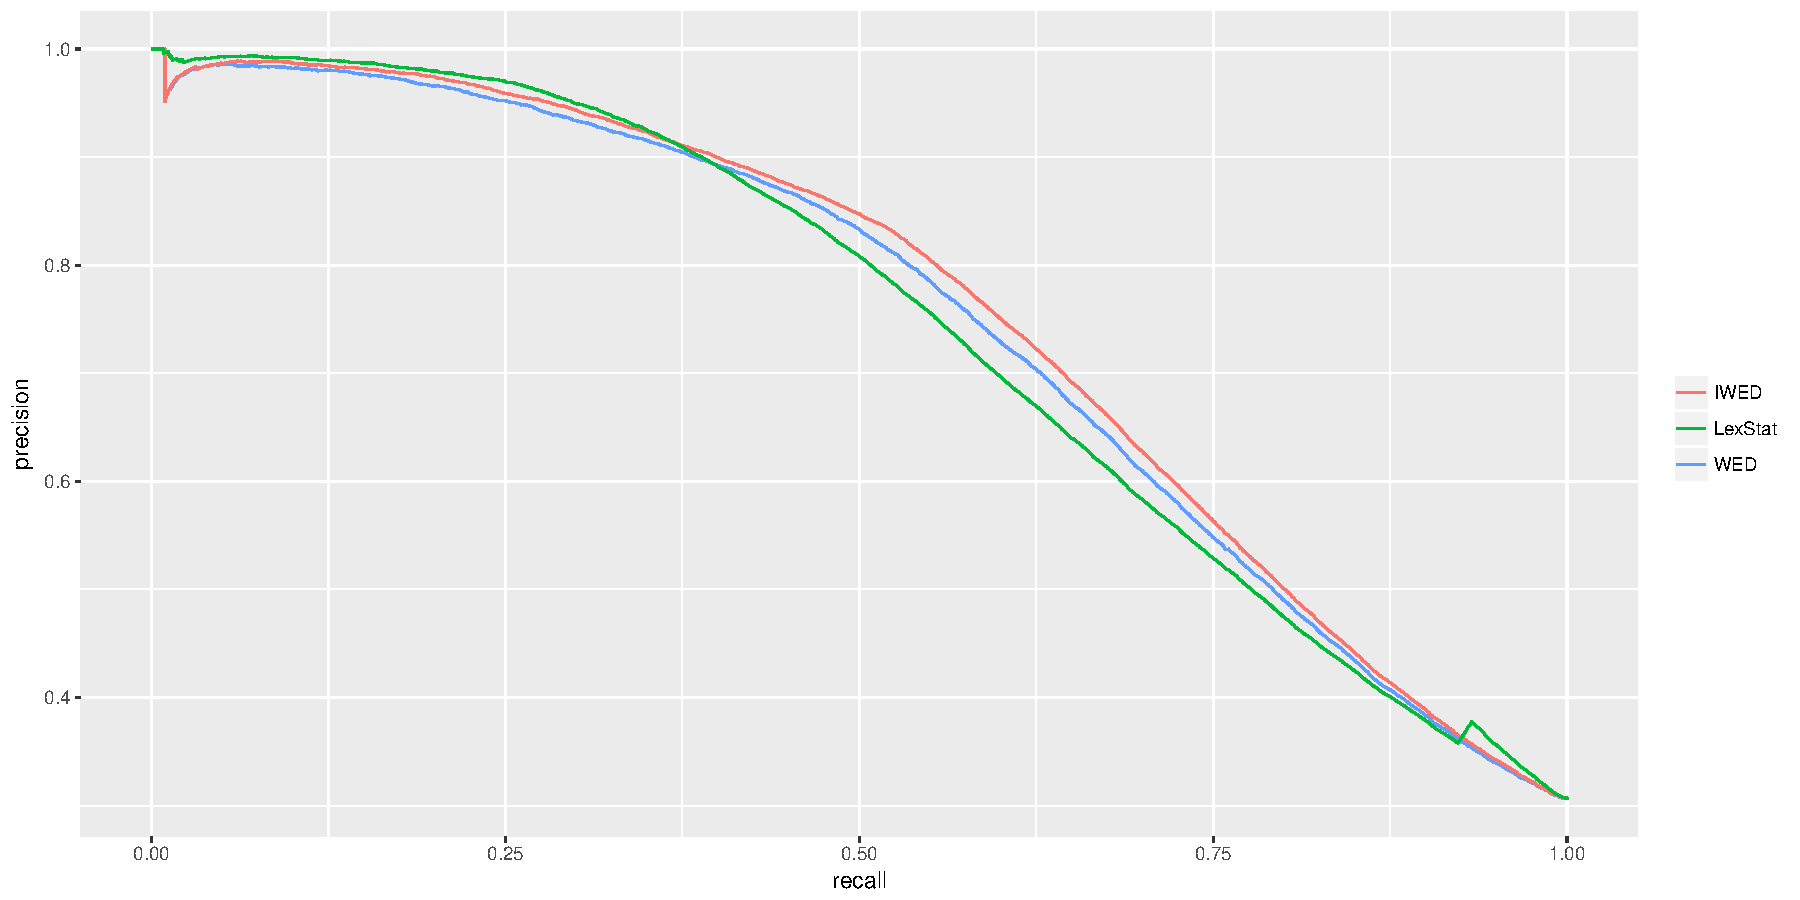
\includegraphics[width=\textwidth]{figures/precision-recall-curves.pdf}
 \caption{Precision-recall curves for cognate detection variants.}
 \label{precision-recall-curves}
\end{figure}

\tabref{average-precision-thresholds} includes the corresponding average precision values, which is defined as the precision integrated over all possible recall values. This gives us a possibility to quantify and compare performance independently of the choice of threshold value. According to this measure, IWD is better than WED, which in turn performs better than LexStat.

\begin{table}
 \centering
 \begin{tabular}{lccc}
  \hline \hline
  Method & LexStat & WED & IWD\\
  \hline
  Average Precision & 0.733 & 0.747 & \textbf{0.766}\\
  \hline
  Threshold for max. F-score & 0.831 & 0.590 & 0.591\\
  Maximal F-score & 0.630 & 0.662 & \textbf{0.681}\\
  \hline
  Threshold for 85\% Precision & 0.737 & 0.495 & 0.462\\
  F-score at 85\% Precision & 0.585 & 0.612 & \textbf{0.632}\\
  \hline
  Threshold for 90\% Precision & 0.698 & 0.430 & 0.387\\
  F-score at 90\% Precision & 0.544 & 0.537 & \textbf{0.556}\\
  \hline
 \end{tabular}
 \caption{Quantitative comparison and data for motivating the thresholds chosen for cognate detection}
 \label{average-precision-thresholds}
\end{table}

The remaining entries of the table contain the necessary numbers for motivating our threshold decisions for IWD and LexStat. If we had no preference for either recall or precision, we could simply maximize the F-score. However, since spurious cognates are a lot more problematic for lexical flow than unrecognized deep cognacy, we want to select for high precision. The figure shows the threshold values corresponding to accuracy values of 85\% and 90\%, and the F-score that can be achieved by choosing that threshold value. It turns out that our initial choice of 0.45 for IWD, and the recommendation of 0.7 for LexStat, are in the range that should lead to precision in the desired range. To avoid overfitting to what also constitutes our test set, I only take this information as confirming the initial decisions, and do not optimize the threshold values further.

The already mentioned \isi{B-Cubed measures} have become the standard for cognate detection since \cite{hauer_kondrak_2011} used them for evaluation, demonstrating the usefulness of measures which go beyond pairwise comparison by taking the inferred clusters into account. For a single word, a recall measure can be defined as the percentage of gold-standard cognates (including the word itself) which occur together with the word in the same result cluster, and an analogous precision measure for each word as the percentage of words in the result cluster which are cognates to the word according to the gold standard. B-Cubed precison and recall are the averages of these clustering accuracy measures across words, and the B-Cubed F-score is again the harmonic mean of B-Cubed precision and recall. To make my results comparable to the recent literature on cognacy detection, I compute these measures in addition to the pairwise performance measures explained above.

The values of all six evaluation measures for the chosen threshold values are given in \tabref{lingpyComparisonIELex}. The numbers show an insignificant advantage of half a percentage point in B-Cubed F-score for LexStat, indicating that IWSA and LexStat perform almost exactly equally well on IPA-encoded dictionary forms for intra-family cognacy judgments. Note that this task is not the one my infrastructure is designed to be particularly good at, so that this evaluation merely shows that on dictionary forms, my system keeps up with the state-of-the-art systems for general cognate detection.

\begin{table}
 \centering
\begin{tabular}{lcccccc}
  \hline \hline
  & \multicolumn{3}{c}{Pairwise} & \multicolumn{3}{c}{B-Cubed}\\
  Method & precision & recall & F-score & precision & recall & F-score\\ \hline
  IWD-0.45 & 0.927 & 0.429 & 0.586 & 0.887 & 0.518 & 0.654\\
  LexStat-0.7 & 0.929 & 0.434 & 0.591 & 0.885 & 0.526 & 0.660\\
  \hline
 \end{tabular}
 \caption{Comparing cognate clustering performance on the intersection of IELex and NorthEuraLex}
 \label{lingpyComparisonIELex}
\end{table}

\subsection{Evaluation on WOLD cross-family cognacy judgments}
To conclusively demonstrate that the infrastructure presented in this chapter is better than the current version of LingPy for the purposes of cross-family cognate detection, a test set which includes cognacy judgments for a dataset which spans multiple families would be necessary. Since such datasets do not currently exist, evaluation must resort to the second-best option of complementing the family-internal evaluation provided by IELex by an evaluation on at least some cognate sets which range across family boundaries.

Fortunately, since cross-family cognates are invariably loanwords (except for a few cases where deep connections are assumed), we can rely on an existing rather comprehensive loanwords database which again has some overlap with the NorthEuraLex data. The World Loanword Database (WOLD)\is{WOLD (World Loanword Database)} was a major data collection effort coordinated by Max Planck Institute for Evolutionary Anthropology in Leipzig, the results of which are summarized in \cite{tadmor2009}. The database is available online \citep{wold}, and was published under a creative commons (CC-BY) license. It contains the realizations of a list of 1460 concepts for a geographically well-balanced sample of 41 languages, and expert judgments on the loanword status for all these words, complete with information on the sources of borrowings. There are eight vocabularies for languages also contained in NorthEuraLex 0.9: \ili{English} \citep{wold-eng}, \ili{Dutch} \citep{wold-nld}, \ili{Romanian} \citep{wold-ron}, \ili{Kildin Saami} \citep{wold-sjd}, \ili{Sakha} \citep{wold-sah}, \ili{Japanese} \citep{wold-jpn}, \ili{Mandarin Chinese} \citep{wold-cmn}, and Ket \citep{wold-ket}. Going through these WOLD vocabularies and extracting all borrowings whose donor languages (or one of their descendants containing reflexes of the same cognate set) are also contained in NorthEuraLex, were not accompanied by a semantic change, and for which the concept was covered by NorthEuraLex, resulted in an evaluation set of 414 loans within NorthEuraLex, of which 214 were intra-family loans, and 200 occurred across family boundaries. This test set is also available as part of the supplementary materials (see Appendix C), to my knowledge providing the first (if modest) benchmark for cross-family cognate detection.

Ideally, we would expect each pair of cognates defined by such a borrowing event to end up in one of the automatically inferred cognate sets. This is what the comparison of the two systems on this dataset was based on. Again, the cognate sets inferred over NorthEuraLex were reduced to a list of pairwise cognacy judgments. Since this dataset provides us with no indication which of the words not affected by borrowing are cognates or not, we unfortunately cannot sensibly compute precision values for this dataset. Instead, I will only rely on the recall values in my evaluation. For a useful comparison, it would usually be a problem if recall is not balanced against precision, but recall still provides meaningful information as long as I keep the parameters fixed, and do not further optimize the system to the new dataset. Using exactly the same system with the threshold values that I demonstrated to be on an equal footing with LingPy on the family-internal cognate classification task, I evaluate whether it manages to detect a higher proportion of cross-family loanwords.

\tabref{lingpyComparisonWOLD} shows the results of the comparison. Since loans are phonetically more similar than the reflexes of inherited cognates, it comes as no surprise that the recall values are higher than in the previous experiment. The interesting finding is in the comparion of intra-family and cross-family loans. In contrast to the IELex data, there is a clear advantage for my system on intra-family loans, probably due to the fact that LexStat requires the existence of sound correspondences, which are of course only partially adhered to by loanwords. The most significant difference is visible in the cross-family loans. Here, LingPy recognizes less than 60\% of the cross-family loans as cognates, whereas my system recognizes cognacy for almost 65\% of pairs. The reason for the difference is that LingPy's infrastructure is dependent on the existence of regular sound correspondences, which is not a problem if the task is to find true cognates within a single family, as was the case in all datasets 
that LingPy has previously been evaluated on \citep{list_ea_2017}. Taking the minimum of global and pair-specific phoneme distances makes my system much more flexible in this regard, while still maintaining a competitive performance for intra-family cognate detection. 

The results indicate that while for the within-family cognacy detection task, the systems show equal performance, my infrastructure seems clearly preferable for preparing cross-family cognacy datasets, the essential preprocessing step for cognacy-based lexical flow inference. In theory, my system might of course also cluster together many more cross-family non-cognate pairs than LingPy, causing precision (which we have no way of measuring) to be much lower than for LingPy, but I would consider that very unlikely given the very similar precision values on the IELex data. Still, it will of course be worthwhile to revisit this issue once larger fully annotated cross-family datasets become available, which would require massive data collection efforts on an even larger scale than the WOLD project.

\begin{table}
 \centering
\begin{tabular}{lcc}
  \hline \hline
  method & recall on intra-family loans & recall on cross-family loans\\ \hline
  LexStat-0.7 & 0.768 & 0.594\\
  IWD-0.45 & 0.888 & 0.645\\
  \hline
 \end{tabular}
 \caption{Comparing cognacy judgments on cross-family loans from the World Loanword Database (WOLD)}
 \label{lingpyComparisonWOLD}
\end{table}

\subsection{A look at the cognate sets}
To illustrate the quality of the results, and the type of data hidden behind everything which is yet to follow, we inspect the NorthEuraLex data and the inferred cognate sets for the concept \textsc{fish} in detail. \figref{cognate-sets-example} contains the standardized IPA representations for all of the NorthEuraLex languages, grouped into cognate sets using UPGMA on my distance measure. I will use the given numbering from 1 to 38 to refer to the cognate sets in the discussion.

\begin{figure}[p!]
\centering \footnotesize
\begin{tabular}{clllll} \hline 
1 & \texttt{gld}: \ipa{[sOgdata]} & & & & \\ 
\hline 
2 & \texttt{kor}: \ipa{[mulgogi]} & & & & \\ 
\hline 
3 & \texttt{sah}: \ipa{[balWk]} & \texttt{tat}: \ipa{[bal7k]} & \texttt{dar}: \ipa{[baliq]} & \texttt{bak}: \ipa{[balWq]} & \texttt{chv}: \ipa{[pul@]} \\ 
 & \texttt{azj}: \ipa{[bAlWg]} & \texttt{kaz}: \ipa{[bAl@q]} & \texttt{uzn}: \ipa{[baliq]} & \texttt{tur}: \ipa{[balWk]} & \\ 
\hline 
4 & \texttt{yux}: \ipa{[Anil]} & & & & \\ 
\hline 
5 & \texttt{slk}: \ipa{[riba]} & \texttt{bul}: \ipa{[riba]} & \texttt{ces}: \ipa{[rIba]} & \texttt{pol}: \ipa{[R1ba]} & \texttt{ukr}: \ipa{[rIbA]} \\ 
 & \texttt{bel}: \ipa{[r1ba]} & \texttt{rus}: \ipa{[r1b@]} & \texttt{hrv}: \ipa{[riba]} & \texttt{slv}: \ipa{[riiba]} & \\ 
\hline 
6 & \texttt{eus}: \ipa{[arAjn]} & & & & \\ 
\hline 
7 & \texttt{kal}: \ipa{[aalisaGaq]} & \texttt{ykg}: \ipa{[al\super jKa]} & & & \\ 
\hline 
8 & \texttt{evn}: \ipa{[ollo]} & & & &\\ 
\hline 
9 & \texttt{heb}: \ipa{[dag]} & & & &\\ 
\hline 
10 & \texttt{fra}: \ipa{[pwasO\~{}]} & \texttt{cym}: \ipa{[p@sgOd]} & & &\\ 
\hline 
11 & \texttt{ket}: \ipa{[ULd \super jiC]} & & & &\\ 
\hline 
12 & \texttt{pes}: \ipa{[m66hi]} & \texttt{pbu}: \ipa{[mAhaj]} & \texttt{hin}: \ipa{[m@tsj]} & \texttt{mal}: \ipa{[matsjam]} & \\ 
\hline 
13 & \texttt{oss}: \ipa{[k@sag]} & \texttt{bre}: \ipa{[pEsk]} & \texttt{isl}: \ipa{[fIskYr]} & \texttt{gle}: \ipa{[I@s\super Gk]} & \texttt{nor}: \ipa{[fIsk]}\\ 
 & \texttt{sqi}: \ipa{[pESk]} & \texttt{dan}: \ipa{[fesg]} & \texttt{lat}: \ipa{[pIskIs]} & \texttt{swe}: \ipa{[fIssk]} &\\
\hline 
14 & \texttt{lit}: \ipa{[ZUV\super jIs]} & \texttt{lav}: \ipa{[zifs]} & & &\\ 
\hline 
15 & \texttt{ava}: \ipa{[t\t{tS}uQa]} & & & &\\ 
\hline 
16 & \texttt{ddo}: \ipa{[besuro]} & & & &\\ 
\hline 
17 & \texttt{hin}: \ipa{[m@\t{tS}\super hlii]} & \texttt{ben}: \ipa{[ma\t{tS}\super h]} & & &\\ 
\hline 
18 & \texttt{hye}: \ipa{[\t{dz}uk]} & & & &\\ 
\hline 
19 & \texttt{kat}: \ipa{[t\super hEvzi]} & & & &\\ 
\hline 
20 & \texttt{bsk}: \ipa{[\t{tC}\super humO]} & & & &\\ 
\hline 
21 & \texttt{kpv}: \ipa{[\t{tC}eri]} & \texttt{koi}: \ipa{[\t{tC}\super jeri]} & \texttt{che}: \ipa{[\t{tS}’@r@]} & \texttt{tel}: \ipa{[\t{tC}eep2]} & \texttt{ain}: \ipa{[\t{ts}ep]}\\ 
\hline 
22 & \texttt{kmr}: \ipa{[masi]} & \texttt{enf}: \ipa{[kari]} & & &\\ 
\hline 
23 & \texttt{mnc}: \ipa{[nimaxa]} & & & &\\ 
\hline 
24 & \texttt{jpn}: \ipa{[sakana]} & \texttt{arb}: \ipa{[samak]} & & &\\ 
\hline 
25 & \texttt{ckt}: \ipa{[@nneen]} & & & &\\ 
\hline 
26 & \texttt{niv}: \ipa{[c\super ho]} & \texttt{cmn}: \ipa{[y]} & & &\\ 
\hline 
27 & \texttt{mns}: \ipa{[Xul]} & \texttt{hun}: \ipa{[h6l]} & \texttt{sme}: \ipa{[kUOlli]} & \texttt{sjd}: \ipa{[kuuLL]} & \texttt{sma}: \ipa{[k0EliE]}\\
 & \texttt{mrj}: \ipa{[kol]} & \texttt{mdf}: \ipa{[kal]} & \texttt{nio}: \ipa{[kol1]} & \texttt{krl}: \ipa{[kAlA]} & \texttt{olo}: \ipa{[kAlA]}\\
 & \texttt{fin}: \ipa{[kAlA]} & \texttt{sel}: \ipa{[q\ae l1]} & \texttt{ekk}: \ipa{[kAlA]} & \texttt{smj}: \ipa{[gUuOllE]} & \texttt{yrk}: \ipa{[xALA]}\\
 & \texttt{myv}: \ipa{[kal]} & \texttt{vep}: \ipa{[kAlA]} & \texttt{mhr}: \ipa{[kol]} & \texttt{liv}: \ipa{[kAlAA]} & \texttt{smn}: \ipa{[kyeli]}\\ 
 & \texttt{kca}: \ipa{[Xu\textbeltl ]} & \texttt{ale}: \ipa{[qAX]} & \texttt{sms}: \ipa{[kuEll\super j9]} & \\ 
\hline 
28 & \texttt{pbu}: \ipa{[kab]} & & & &\\ 
\hline 
29 & \texttt{kan}: \ipa{[miinu]} & \texttt{tam}: \ipa{[miin]} & & &\\ 
\hline 
30 & \texttt{bua}: \ipa{[zagahaN]} & \texttt{khk}: \ipa{[\t{ts}a\;Gas]} & \texttt{xal}: \ipa{[\t{ts}a\textcrh s5n]} & &\\ 
\hline 
31 & \texttt{udm}: \ipa{[\t{tC}or1g]} & \texttt{abk}: \ipa{[Ap\super hs1\t{dz}]} & & &\\ 
\hline 
32 & \texttt{itl}: \ipa{[@\textltailn \t{tS}]} & & & &\\ 
\hline 
33 & \texttt{deu}: \ipa{[fIS]} & \texttt{eng}: \ipa{[fIS]} & \texttt{nld}: \ipa{[vIs]} & \texttt{ket}: \ipa{[jiC]} &\\ 
\hline 
34 & \texttt{por}: \ipa{[pejS@]} & \texttt{cat}: \ipa{[pES]} & \texttt{ita}: \ipa{[peSSe]} & \texttt{ron}: \ipa{[peSte]} & \texttt{spa}: \ipa{[peT]}\\ 
\hline 
35 & \texttt{lbe}: \ipa{[\t{tS}awa\t{qX}]} & & & &\\ 
\hline 
36 & \texttt{ell}: \ipa{[psari]} & \texttt{ady}: \ipa{[p\t{ts}a\:z@j]} & & &\\ 
\hline 
37 & \texttt{ess}: \ipa{[iqa\t{t\textbeltl}juk]} & & & &\\ 
\hline 
38 & \texttt{lez}: \ipa{[Ked]} & & & &\\ 
\hline 
\end{tabular}
\caption{Inferred cognate sets and NorthEuraLex forms for \textsc{fish}}
\label{cognate-sets-example}
\end{figure}

The largest inferred cognate set 27 correctly clusters a large number of Uralic\il{Uralic languages} words, all of which derive from Proto-Uralic \textit{*kala}. Note that the algorithm sucessfully detects the regular alternation between Western Uralic \ipa{[k]}, Ob-Ugric \ipa{[X]}, and \ili{Hungarian} \ipa{[h]}, as well as the large variety of diphthongs in the Saami reflexes. However, set 27 also contains a false positive: \ili{Aleut} \ipa{[qAX]} actually belongs together with \ili{Siberian Yupik} \ipa{[iqa\t{t\textbeltl}juk]} (set 37), both going back to Proto-Eskimo-Aleut \ipa{*iqa{\textbeltl}uG}, which might actually be deeply related to the Uralic word according to \citet[footnote 51]{fortescue1998}. This would make the inclusion of the Aleut word in this cluster an instance of successful deep cognacy detection, although of course the phonologically closer Yupik word is missing. The \ili{Udmurt} form \ipa{[\t{tC}or1g]} in set 31 actually belongs to the other Permian forms in set 21, which again 
erroneously includes the \ili{Chechen} word \ipa{[\t{tS}’@r@]}, an impressive instance of chance similarity with \ili{Komi-Zyrian} \ipa{[\t{tC}eri]}. Set 21 also includes the non-cognate, but phonetically similar words from \ili{Ainu} and \ili{Telugu}.

The situation of the words for \textsc{fish} in Indo-European\il{Indo-European languages} is much more complicated than in Uralic. The most important set comprising the Western branches of Indo-European, ultimately going back to a PIE form \textit{*pis\'{k}-}, decomposes into several sets (10, 13, 33, 34) in the automated clustering. The main problem is that due to the one-to-one correspondence model, the bigram \ipa{[sk]} cannot be matched to the single segment \ipa{[S]} which it is reflected by in West Germanic (cluster 33, with \ili{Ket} \ipa{[jiC]} erroneously added due to the rhyme). The separate development into \ipa{[S]} in some \ili{Romance languages} led to an additional cluster (set 34), which cannot be integrated with cluster 33 due to the additional imperfect match between \ipa{[p]} and \ipa{[f]} in the first segment, although this is due to a regular sound correspondence. \ili{Welsh} \ipa{[p@sgOd]} in set 10 is indeed a loan from Romance, and is thus not particularly close to its \ili{Irish} 
equivalent \ipa{[I@s\super Gk]} in set 13.

Pokorny's Eastern Indo-European root \textit{*\'{g}dʰ\={u}-} is reflected in NorthEuraLex by the Baltic\il{Baltic languages} words (set 14) and the \ili{Armenian} word (set 18), which would thus form a single cluster in an ideal result. However, this reconstruction is not uncontested, so that it is equally acceptable for the words to form separate clusters. The Slavic\il{Slavic languages} innovation \textit{*ryba} (set 5) and the Indo-Iranian\il{Indo-Iranian languages} substrate word \textit{*m\'{a}tsyas} (sets 12 and 17) are reliably and correctly detected as outliers, although the latter set is split in half due to an undetectable multi-segment sound change from \ili{Sanskrit} \ipa{[tsj]} (reflected by \ili{Hindi} and \ili{Malayalam} loans in set 12) to \ipa{[\t{tS}\super h]} in Prakrit and the modern \ili{Indo-Aryan languages} (set 17). \ili{Pashto} \ipa{[kab]} (set 28) represents an Eastern Iranian word that might also be reflected by \ili{Ossetian} \ipa{[k@sag]}, which was erroneously 
grouped together with the other Indo-European words in set 13, due to the very similar second and third consonants.

Both the Turkic\il{Turkic languages} (set 3) and the Mongolic\il{Mongolic languages} (set 30) words for \textsc{fish} are reliably clustered together and correctly separated from all the other sets, due to very regular sound correspondences bridging the sometimes highly divergent forms. The inherited Dravidian\il{Dravidian languages} word is detected correctly as well (set 29), and despite the identical initial segment it is correctly not thrown together with the Indo-Iranian word (set 12), even if the latter was additionally borrowed by Malayalam.

According to \cite{nikolayev_starostin_1994}, \ili{Adyghe} \ipa{[p\t{ts}a\:z@j]} (in set 36) and \ili{Abkhaz} \ipa{[Ap\super hs1\t{dz}]} (in set 31) are both reflexes of a Proto-Northwest-Caucasian\il{Northwest Caucasian languages} \textit{*p:ə\v{s}A}, a relationship which is also quite apparent in the surface forms. To Nikolayev and Starostin, who assume the existence of a North Caucasian macrofamily, the first part of \ili{Tsez} \ipa{[besuro]} (set 16) also belongs to this set. Since a common descent of the two language families is not generally accepted as proven, it appears acceptable for the Tsez word to show up as a singleton set.

Coming to the Paleosiberian languages, \cite{fortescue2005} groups the \ili{Chukchi} word \ipa{[@nneen]} (set 25) and Itelmen \ipa{[@\textltailn \t{tS}]} (set 32)  together as reflexes of Proto-Chukotko-Kamchatkan\il{Chukotko-Kamchatkan languages} *\ipa{@nn@}, making this pair of words a false negative. Deciding whether set 7, grouping \ili{Tundra Yukaghir} \ipa{[al\super jKa]} with \ili{Greenlandic} \ipa{[aalisaGaq]}, is acceptable requires some digging into the etymological literature, since the forms are suspiciously similar, and ancient Yukaghir-Eskimo contacts are not unlikely. According to \cite{fortescue_ea_2010}, however, the first two syllables of the Greenlandic form go back to a Proto-Eskimo stem *\ipa{aGula}- `to move', whereas \citet[Lemma 1627]{nikolaeva2006} reconstructs Proto-Yukaghir *\ipa{ol\super joG@} in the meaning of `fish', excluding the possibility of a loan.

Unavoidably, there are a number of obvious false positives, typically sets of size two which were clustered together due to some random partial similarity. The instances I would count as such false positives are the sets containing \ili{Kurdish} and \ili{Enets} (set 22), \ili{Japanese} and \ili{Arabic} (set 24), \ili{Udmurt} and \ili{Abkhaz} (set 31), as well as \ili{Greek} and \ili{Adyghe} (set 36).

For the remaining singleton sets (1, 2, 4, 6, 8, 9, 11, 15, 19, 20, 23, 35, 38), I could not find any indication in the etymological literature that some of these should have been clustered together with any other set, so that these can be counted as correct classifications.

From this example and the discussion, it should be obvious that automated cognate clustering across many language families, especially while avoiding false positives, is a very challenging task for a computer if it is not given parts of the expected result (family relationships) as part of the input. Many improvements to the method could be made, like a model which would support multi-segment correspondences, or more sophisticated clustering. Also, having a large portion of the basic vocabulary at one's disposal should make it easier to at least bring some parts of the comparative method to bear on the task of automated cognate detection. Still, it is also clear that despite the presence of noise, there is already a lot of relevant signal even in the words for a single concept. Across 1,016 slices of equal size and similar structure, the false positives will tend to be distributed equally across language pairs, whereas an accumulation of true cognates will make the true affiliations of languages clearly 
visible.

\section{Deriving a gold standard for lexical flow}\label{sec:4.6}
The obvious way to go about evaluating the network inference algorithms is to check how well it concurs with previous knowledge about language contacts in some linguistic regions. For this purpose, I will be using the cognate data derived from NorthEuraLex, and focus on four linguistic areas of interest, which are discussed in detail. For the other NorthEuraLex languages, and the contacts between them, research into the available literature was performed a little more superficially, resulting in a set of 205 language contacts among the 107 NorthEuraLex languages and their ancestors. All the contacts which are part of the gold standard are given in Appendix A.3.

\subsection{Defining the gold standard}
To define the gold standard, the best result we could hope to achieve on the NorthEuraLex data, it was necessary to review literature on the history of all the languages involved, and define a list of language contacts which are likely to have had sufficient influence on the vocabulary covered by NorthEuraLex to still be visible in the cognacy relations.

In principle, we can just decide for each pair of languages whether they have a common ancestor (which would correspond to a \arrowAA edge), or whether there has been lexical transfer between unrelated languages. As argued in the discussion of the simulation model, for basic vocabulary lexical transfer will virtually always have a dominant direction, giving rise to \arrowLA edges in the gold standard. Finally, there is the case of languages which belong to the same family (have a distant common cause), but have exchanged substantial amounts of lexical material later in their development. The prime example case for this could be the relation between \ili{English} and \ili{French}. Proto-Indo-European certainly qualifies as an unobserved common cause for both languages (\textit{fra} \arrowAA \textit{eng}). However, the number of such ancient cognates between the two languages which still have the same meaning is quite low compared to the number of cognates both languages share due to massive borrowing from 
French into English since the Norman conquest (\textit{fra} \arrowLA \textit{eng}). Faced with good reasons for accepting both arrow patterns, it seems sensible to do just that during the evaluation. For this particular language pair, it makes sense to accept as valid any ancestral graph with either \textit{fra} \arrowAA \textit{eng} or \textit{fra} \arrowLA \textit{eng}, which can be expressed by reusing PAG notation as \textit{fra} \arrowOA \textit{eng}. Both the absence of an edge between English and French and a wrongly directed edge \textit{eng} \arrowLA \textit{fra} would be counted as errors.

The difficult issue for defining a good gold standard is the treatment of lateral connections between proto-languages, i.e.\ causal influences between the latent variables. For instance, the influence of Proto-Baltic on Proto-Finnic might become visible as a directed arc from any Baltic\il{Baltic languages} to any Finnic language\il{Finnic languages}. On some level, it is wrong to state that \ili{Latvian} influenced \ili{Veps} (\textit{lav} \arrowLA \textit{vep}), but the alternative (\textit{lav} \arrowAA \textit{vep}), while technically more justified, is problematic as well, because it blurs the distinction between ancient relationship and contact that we would like our algorithms to detect. For this reason, I will collect contact relationships between larger phylogenetic units (\textit{Eastern Baltic} \arrowLA \textit{Finnic}), and compile them out into statements connecting the attested languages (\textit{lav} \arrowLA \textit{vep}, \textit{lit} \arrowLA \textit{vep}, \textit{lav} \arrowLA \textit{fin}, 
\textit{lit} \arrowLA \textit{fin}, \dots) for the contact flow evaluation. While this makes it easy to evaluate precision (essentially, any directed contact from a Baltic to a Finnic language is accepted as correct), it complicates the definition of recall. Do we expect each lexical transfer between proto-languages to be represented as an arrow between one pair of descendant languages in the result? What if due to further events on both involved families, the lexical transfer is barely visible in the observed languages? For the simulated data, we have a full model of the ground truth, and can define precise threshold values to decide which ancient contacts we would expect to still be detectable. For the real data, this task would amount to compiling full etymological information for the entire database, which is a worthwhile long-term goal, but completely unfeasible for a single person in a few years. Therefore, selection of contact events which we expect to find represented has to build on aggregated 
statements about the amount of lexical influence in the literature, and estimates how well the affected layers of the lexicon are actually represented in the data. Moreover, all kinds of biases might be introduced as a result of an uneven distribution of research effort, which can result from all kinds of extralinguistic factors, from a very local bias like an individual researcher's aesthetic preferences to very global biases if, e.g. for political reasons, it is easier for researchers from one country to get funding for work on the contacts with one neighboring nation over another. My gold standard derived from available literature might therefore well be incomplete, but it still contains a large number of contact events which are so clearly visible in the data that any automated system which tries to infer directional contact should be able to find them.

In the linguistic overviews accompanying the four case studies using subsets of NorthEuraLex which are described in the following sections, I will state each contact event that is included in my overall gold standard for NorthEuraLex (again available as part of the supplementary materials) in brackets after the point which justifies it. For instance, English borrowed some basic vocabulary from North Germanic during the Viking settlement (\textit{North Germanic} \arrowOA \textit{eng}), and was heavily influenced by French after the Norman conquest (\textit{fra} \arrowOA \textit{eng}). I also state the NorthEuraLex representatives of each phylogenetic unit the first time I mention it, e.g.\ North Germanic (\textit{isl}, \textit{nor}, \textit{swe}, \textit{dan}).

\subsection{Case study 1: the Baltic Sea area}
The first case study on real data will deal with the languages around the Baltic sea, which is a comparatively easy case because only two language families are involved (Indo-European and Uralic), and almost all instances of language contact occurred among neighbors, or across the sea, without migrations complicating the picture. The linguistic history of the region is thus not very involved, but still complex enough to provide some interesting test cases for lexical flow inference.

The basic linguistic layout of the lands around the Baltic sea is that of a border region where the Indo-European languages of central and eastern Europe meet the westernmost Uralic languages. For a comprehensive overview of the linguistic history of this region, the reader is referred to the volume on Circum-Baltic languages as an areal grouping, edited by \cite{dahl_koptjevskaja-tamm_2001}, from where some of the information in this overview is taken. \figref{baltic-cognacy} visualizes the NorthEuraLex languages around the Baltic sea at their rough geographical coordinates, with the overlap in inferred cognate sets between each language pair visualized by a line, which gets thicker and less transparent with the amount of overlap. This cognacy strength visualization is a convenient way to summarize the shape of the lexical flow inference problem.

\begin{figure}
 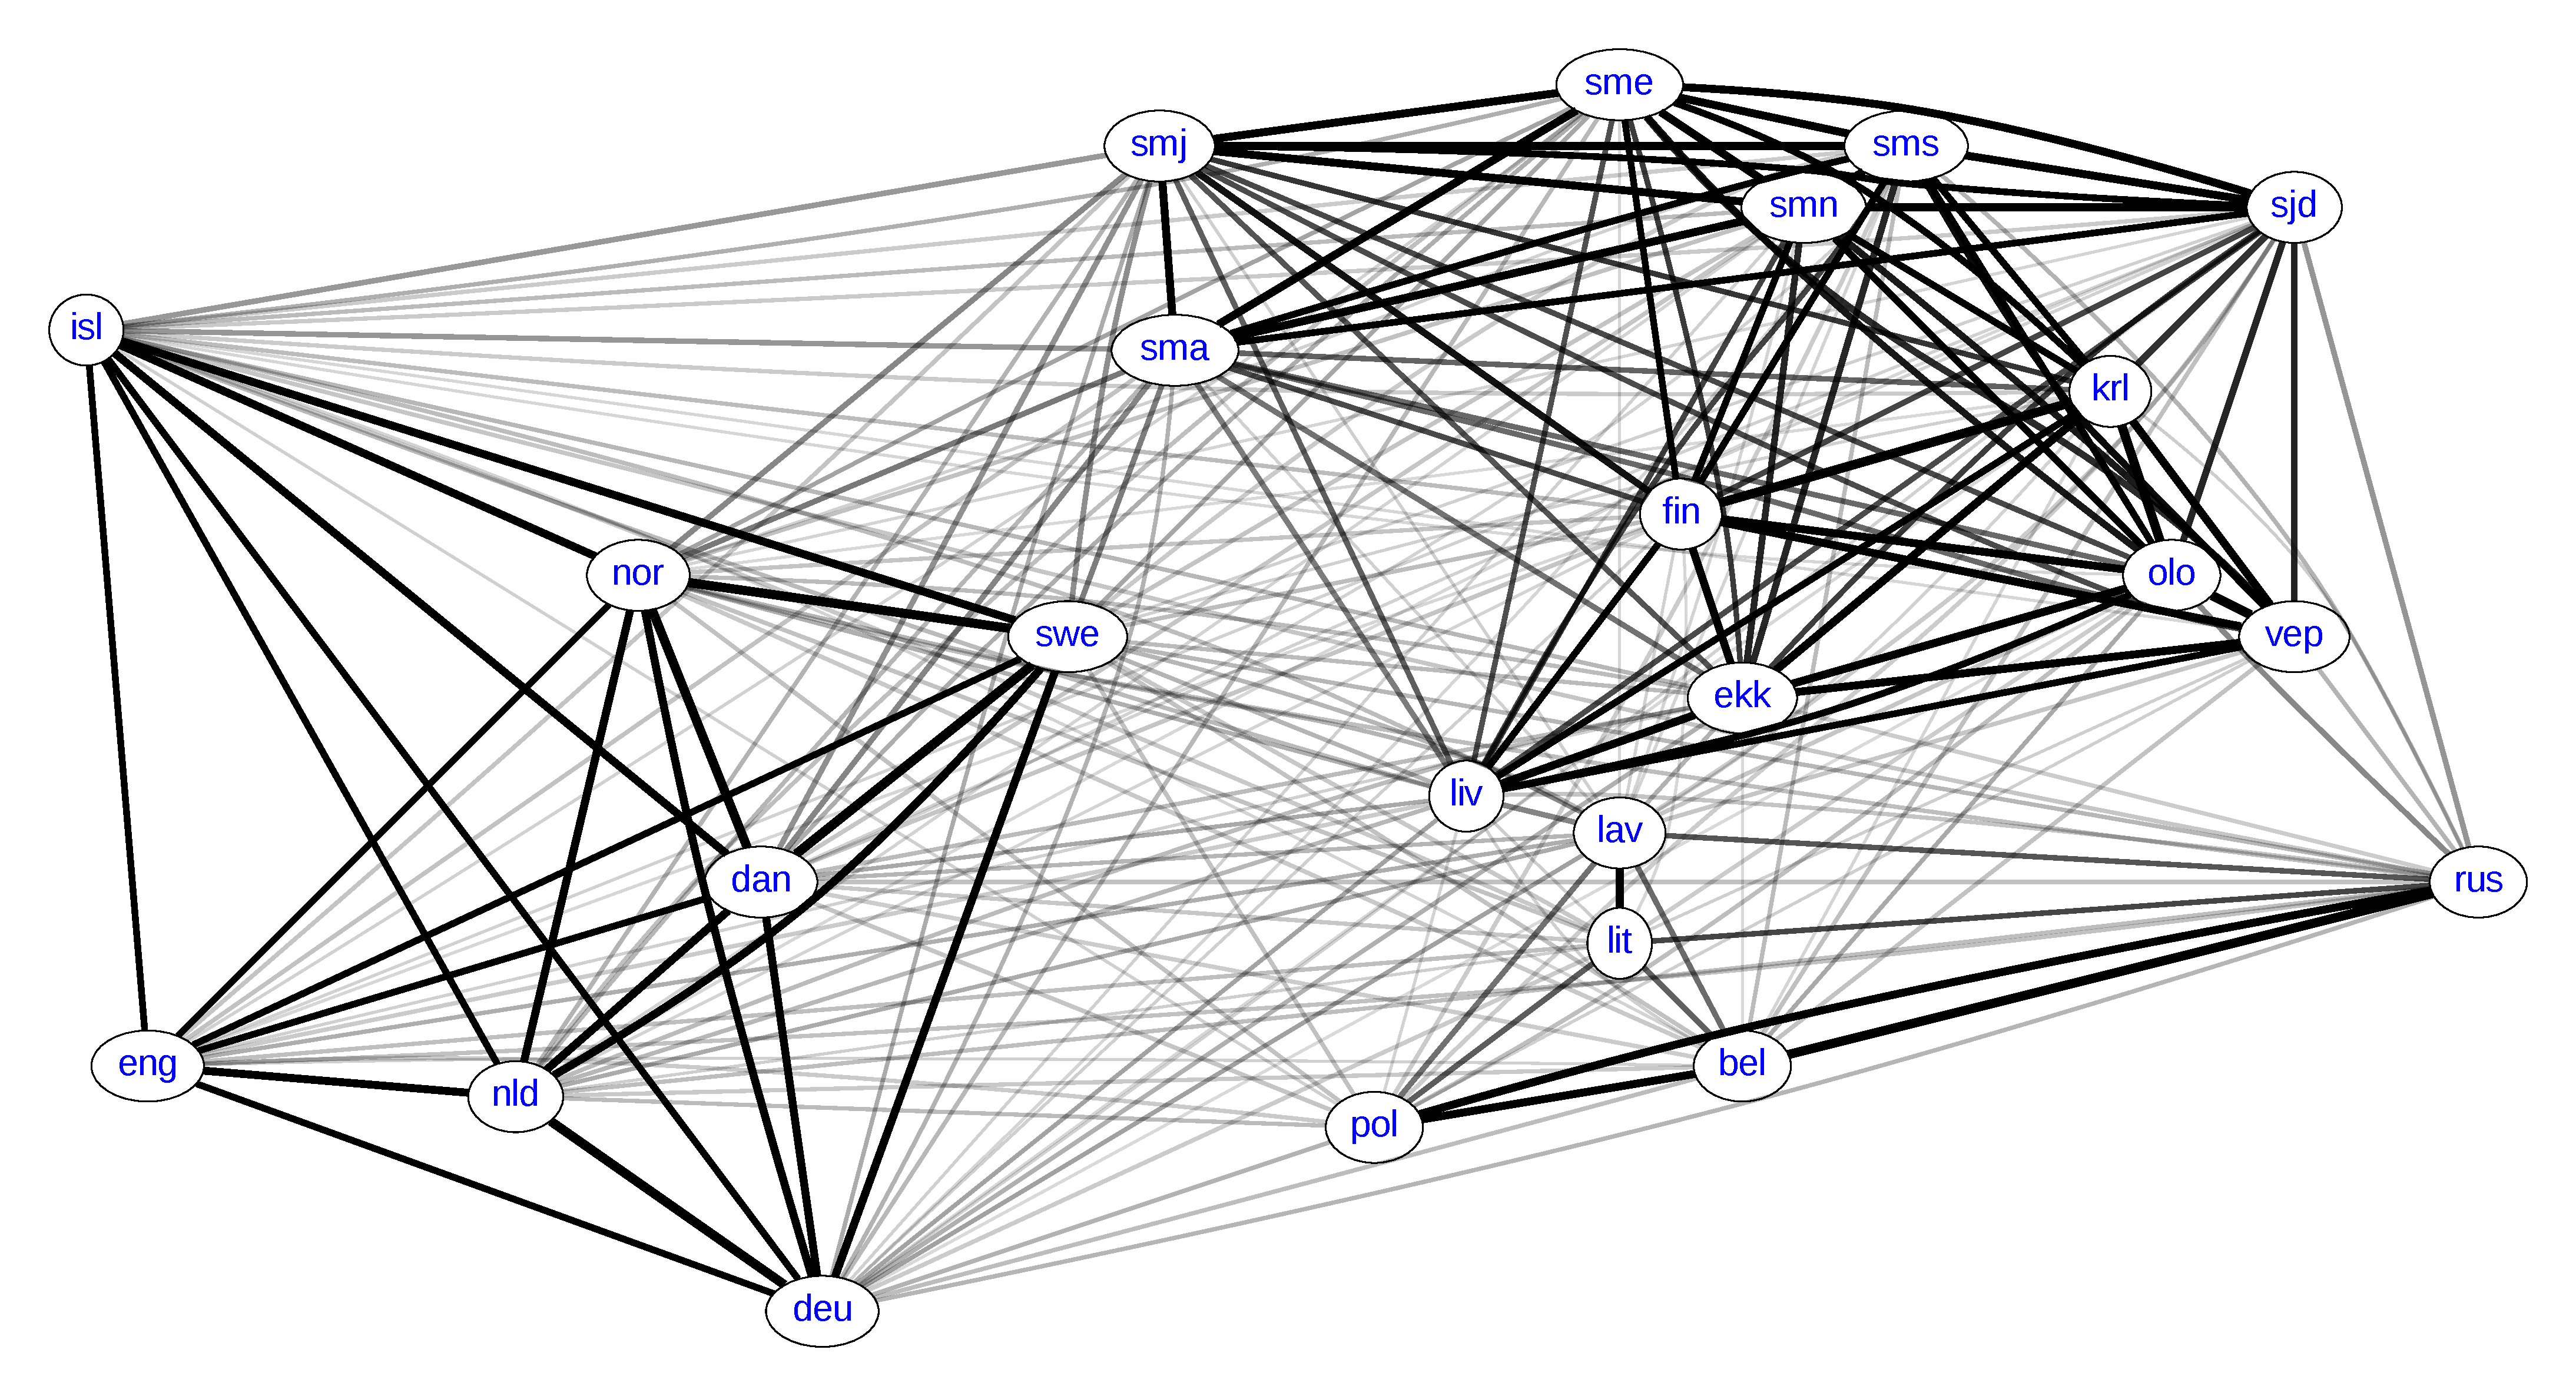
\includegraphics[width=\textwidth]{figures/cognacy-strength-baltic.pdf}
 \caption{Visualization of inferred cognate overlap in the Baltic Sea data}
 \label{baltic-cognacy}
\end{figure}

On the Indo-European side, southern Scandinavia is the homeland of the \ili{North Germanic languages} (\textit{swe}, \textit{dan}, \textit{nor}, \textit{isl}), which have evolved from the \ili{Old Norse} of the Viking Age, whose Western dialect developed into the West Scandinavian languages \ili{Icelandic} (\textit{isl}), \ili{Faroese}, and \ili{Norwegian} (\textit{nor}), whereas the Eastern dialect gave rise to \ili{Danish} (\textit{dan}) and \ili{Swedish} (\textit{swe}). The position of Norwegian in this genealogical tree is a little problematic, because Norwegian has a lot of dialectal variation, and two quite different written standards. The \ili{Nynorsk} standard can, with some justification, still be called a West Scandinavian language, whereas the \ili{Bokm\aa{}l} variant represented in NorthEuraLex is much more similar to the East Scandinavian languages. As another native language of the region of high historical significance, \ili{German} (\textit{deu}), which belongs to the West Germanic branch, is 
also part of this case study. From a historical perspective, it would have made more sense to include \ili{Low German} instead of Standard High German, but no variant of Low German is featured in NorthEuraLex so far.

The only \ili{Slavic languages} with any relevance for the Baltic sea region are \ili{Polish} (\textit{pol}) as well as \ili{Russian} (\textit{rus}) and closely related \ili{Belarusian} (\textit{bel}). The Slavs originally settled a homeland somewhere in Eastern Poland or Western Ukraine, and began their rapid expansion in all directions as late as 500 AD \citep{kobylinski2005}. In later centuries, when Russian had become the state language of a great power with major strategic interests in the region, it started to exert a dominating influence on all languages on the eastern coast of the Baltic sea as well \citep{decsy1988}. \cite{smolicz_radzik_2004} summarize how during its short history, literary Belarusian has continually been remolded to be either lexically closer to Polish (\textit{pol} \arrowOA \textit{bel}) or to Russian (\textit{rus} \arrowOA \textit{bel}) depending on the political situation, and show that its present role, despite being the titular state language of Belarus, is in many ways more 
similar to an endangered minority language.

The \ili{Baltic languages}, which show so much similarity with the Slavic languages that a single Balto-Slavic branch of Indo-European is generally assumed, once settled a large area north of the Slavs, but have since been gradually displaced by expanding Germans and Slavs, except for two surviving languages of the Eastern Baltic branch, \ili{Lithuanian} (\textit{lit}) and \ili{Latvian} (\textit{lav}), which are the national languages of the respective modern states. \ili{Old Prussian}, the ancient language of Prussia which became extinct through replacement with German in the 18th century, is the single relatively well attested Western Baltic language, but it cannot be included in NorthEuraLex because information on only a fraction of the relevant concepts is available.

According to \cite{viitso1998}, the \ili{Finnic languages} (\textit{fin}, \textit{krl}, \textit{olo}, \textit{vep}, \textit{ekk}, \textit{liv}) form an ancient dialect continuum reaching around the Gulf of Finland, where \ili{Finnish} (\textit{fin}) and Standard \ili{Estonian} (\textit{ekk}) became national languages during the 19th century, and others have survived as small minority languages of northwestern Russia, predominantly in the Republic of Karelia. Of these smaller languages, NorthEuraLex contains two written variants of \ili{Karelian} (\ili{North Karelian} \textit{krl} and \ili{Olonets Karelian} \textit{olo}), and the \ili{Veps} language (\textit{vep}). Moreover, NorthEuraLex contains data for the recently extinct \ili{Livonian} (\textit{liv}) of Latvia.

The \ili{Saami languages} (\textit{sma}, \textit{smj}, \textit{sme}, \textit{smn}, \textit{sms}, \textit{sjd}) form another ancient dialect continuum \citep{sammallahti1998} across northernmost Scandinavia, which is conventionally split into at least ten languages, six of which have standardized literary variants. Western Saami (\textit{sma}, \textit{smj}, \textit{sme}) consists of \ili{Southern Saami} (\textit{sma}), \ili{Lule Saami} (\textit{smj}), and \ili{Northern Saami} (\textit{sme}), which is by far the most thriving of the Saami languages, and is becoming a lingua franca for all Saami speakers due to its large number of speakers, the central position it takes in the dialect continuum, and its state-sponsored role as a media and academic language. The Eastern Saami languages (\ili{Inari Saami} \textit{smn} and \ili{Skolt Saami} \textit{sms} in Finland, as well as \ili{Kildin Saami} \textit{sjd} on the Kola peninsula) are all severely endangered, with only a few hundred speakers left for each of them.

As shown by \cite{aikio2006contacts}, already the Nordic Bronze Age culture before 500 BC appears to have had intensive trade contacts with Finnic tribes in the Baltics, and Saami tribes in Finland. During the early Middle Ages, when the Saami had settled Northern Scandinavia, and Southern Finland had been colonized by the Finns, these contacts intensified. After christianization, Swedish settlers started to colonize parts of Finland's coastal areas in the 12th century. The influx of settlers continued into the times of the Northern Crusades, as a result of which Western Finland became part of the Swedish state. \ili{Swedish} as the language of administration and education had a strong influence on the western dialects of \ili{Finnish}, which later became the basis for the written standard (\textit{swe} \arrowLA \textit{fin}). At the same time, Russian missionaries had started to spread the orthodox faith among the Finnic tribes of the east, which both influenced the later national borders between Swedish 
Finland and Novgorod (and later Russia), and contributed to the concept of separate Finnish and Karelian nationalities. The lexical impact of \ili{Russian} on the \ili{Karelian} dialects was of a similar nature as that of Swedish on Finnish in the west (\textit{rus} \arrowLA \textit{krl, olo}). According to \cite{puura_ea_2013}, Russian influence on spoken \ili{Veps} has been quite strong as well due to near-complete bilingualism. In contrast, the recently published dictionaries such as \cite{zajceva2010} are quite purist, which means that only very few Russian loans are visible in the NorthEuraLex data for this language. This hints at a more general problem with representing minority languages in lexical databases. Due to purist attitudes, Russian loans, even if they are the first words that come to mind for certain concepts, will not be accepted as part of their language by dictionaries or native informants, even though the words given instead might already have fallen out of actual use.

\cite{zachrisson2008} provides an overview of later interactions between North Germanic peoples and the Saami. Since the late Middle Ages, when \ili{Saami languages} were still spoken much further to the south, the development of the centralized Scandinavian nation states, and accompanying christianization, has been causing the Saami population to assimilate, or migrate further to the north. For centuries, the language policy of the Scandinavian nation states was to ban the use of Saami languages at school and in public life \citep{corson1995}, which has led to intensive pressure of the North Germanic state languages\il{North Germanic languages} on the \ili{Western Saami languages} (\textit{swe} \arrowLA \textit{Western Saami}, \textit{nor} \arrowLA \textit{Western Saami}). The same pattern, along with its role as a trade language, has led to massive Finnish influence on \ili{Northern Saami} (\textit{fin} \arrowOA \textit{sme}), \ili{Inari Saami} (\textit{fin} \arrowOA \textit{smn}), and, chiefly after the 
Skolts' resettlement during the aftermath of the Second World War \citep{feist2011}, on \ili{Skolt Saami} (\textit{fin} \arrowOA \textit{sms}). The \ili{Eastern Saami languages}, which were once spoken across Karelia, had previously been influenced \citep{sergejeva2000} by neighboring North Karelians (\textit{krl} \arrowOA \textit{Eastern Saami}), and then of course by the Russian state language (\textit{rus} \arrowLA \textit{sjd, sms}).

Some of the earliest language contacts in the region occurred between Finnic and Baltic tribes at a time when the Slavs had not yet expanded to the north. \cite{suhonen1988} lists a large number of ancient Baltic\il{Baltic languages} loans in the \ili{Finnic languages}, covering semantic fields such as basic tools and agriculture, many animal and plant names, and female kinship terms (\textit{Baltic \arrowLA Finnic}). While the frequency of Baltic loans is highest in \ili{Finnish}, \ili{Estonian}, and \ili{Olonets Karelian}, this effect, as Suhonen himself points out, might be simply due to the less well-developed lexicography in the smaller Finnic languages. Moreover, \cite{suhonen1973} counts more than 2,200 recent \ili{Latvian} loans in the \ili{Livonian} language (\textit{lav \arrowLA liv}), an interesting case of overwhelming influence of a written majority language on a barely written minority language, while the majority language is itself but a regional minority language in a much larger state.

In Estonia and Latvia, Hanse traders and especially the crusaders of the Teutonic Order, who founded their state in the Baltics in the 13th century, brought the \ili{German} language with them. As \cite{rot1988} demonstrates, German had an enormous impact on the cultural vocabulary of both the \ili{Estonian} language (\textit{deu} \arrowLA \textit{ekk}) and then still widespread \ili{Livonian} (\textit{deu} \arrowLA \textit{liv}). Some of these words were also borrowed into \ili{Latvian} (\textit{deu} \arrowOA \textit{lav}). Although both countries ended up protestant after the reformation, the early missionary activities by the orthodox church are still visible in the religious vocabularies of both languages, and further influence of the dominant language during Imperial \ili{Russian} and Soviet times has left traces (\textit{rus} \arrowLA \textit{ekk}, \textit{rus} \arrowOA \textit{lav}).

Further to the south, \ili{Lithuanian} was not influenced by German to the extent that the other languages of the Baltics were, due to a separate statehood tradition which aligned Lithuanians more closely with Poland than with their other neighbors. As \cite{senn1944} writes, 16th-century Lithuanian still showed quite a bit of influence of \ili{Polish} and \ili{German}, but most of these loans were removed from the language due to later purist attitudes, such that modern Lithuanian contains almost no borrowings in its basic vocabulary.

On the south coast of the Baltic sea, exchange between Germans and Slavs has led to some mutual influence, which has left the basic vocabulary largely untouched, however. Also, the more recent loans from German into Polish do not exceed a handful among the concepts covered by NorthEuraLex. The influence of German on its much more closely related northern neighbors has been more pronounced, with written German being a strong influence on the development of all three modern written standard languages of Scandinavia (\textit{deu} \arrowOA \textit{dan}, \textit{swe}, \textit{nor}), while Icelandic stayed untouched by these developments due to its isolation. During the centuries of Danish rule over Norway, the more widespread Bokm\aa{}l of the two competing written forms of Norwegian, was very much molded after the model of Danish on every level (\textit{dan} \arrowOA \textit{nor}), which is still visible in the fact that it now resembles its East Scandinavian neighbors much more (to the point of mutual intelligibility) than its West Scandinavian sister language Icelandic.

To summarize, \figref{baltic-goldstandard-phylo} visualizes the gold standard for phylogenetic lexical flow inference on the dataset. The proto-languages are located roughly at their reconstructed positions, with some modifications which had to be made for readability. Inheritance relationships are visualized with black arrows, bidirectional contact with light green lines (not in this case study), and unidirectional contacts are shown as dark green arrows. Sometimes, some arrows will deviate from the gold standard motivated in the text. In such cases, the deviating arrows will represent the closest equivalent to a relevant contact where one of the proto-languages was not present in the reduced tree.

\begin{figure}
 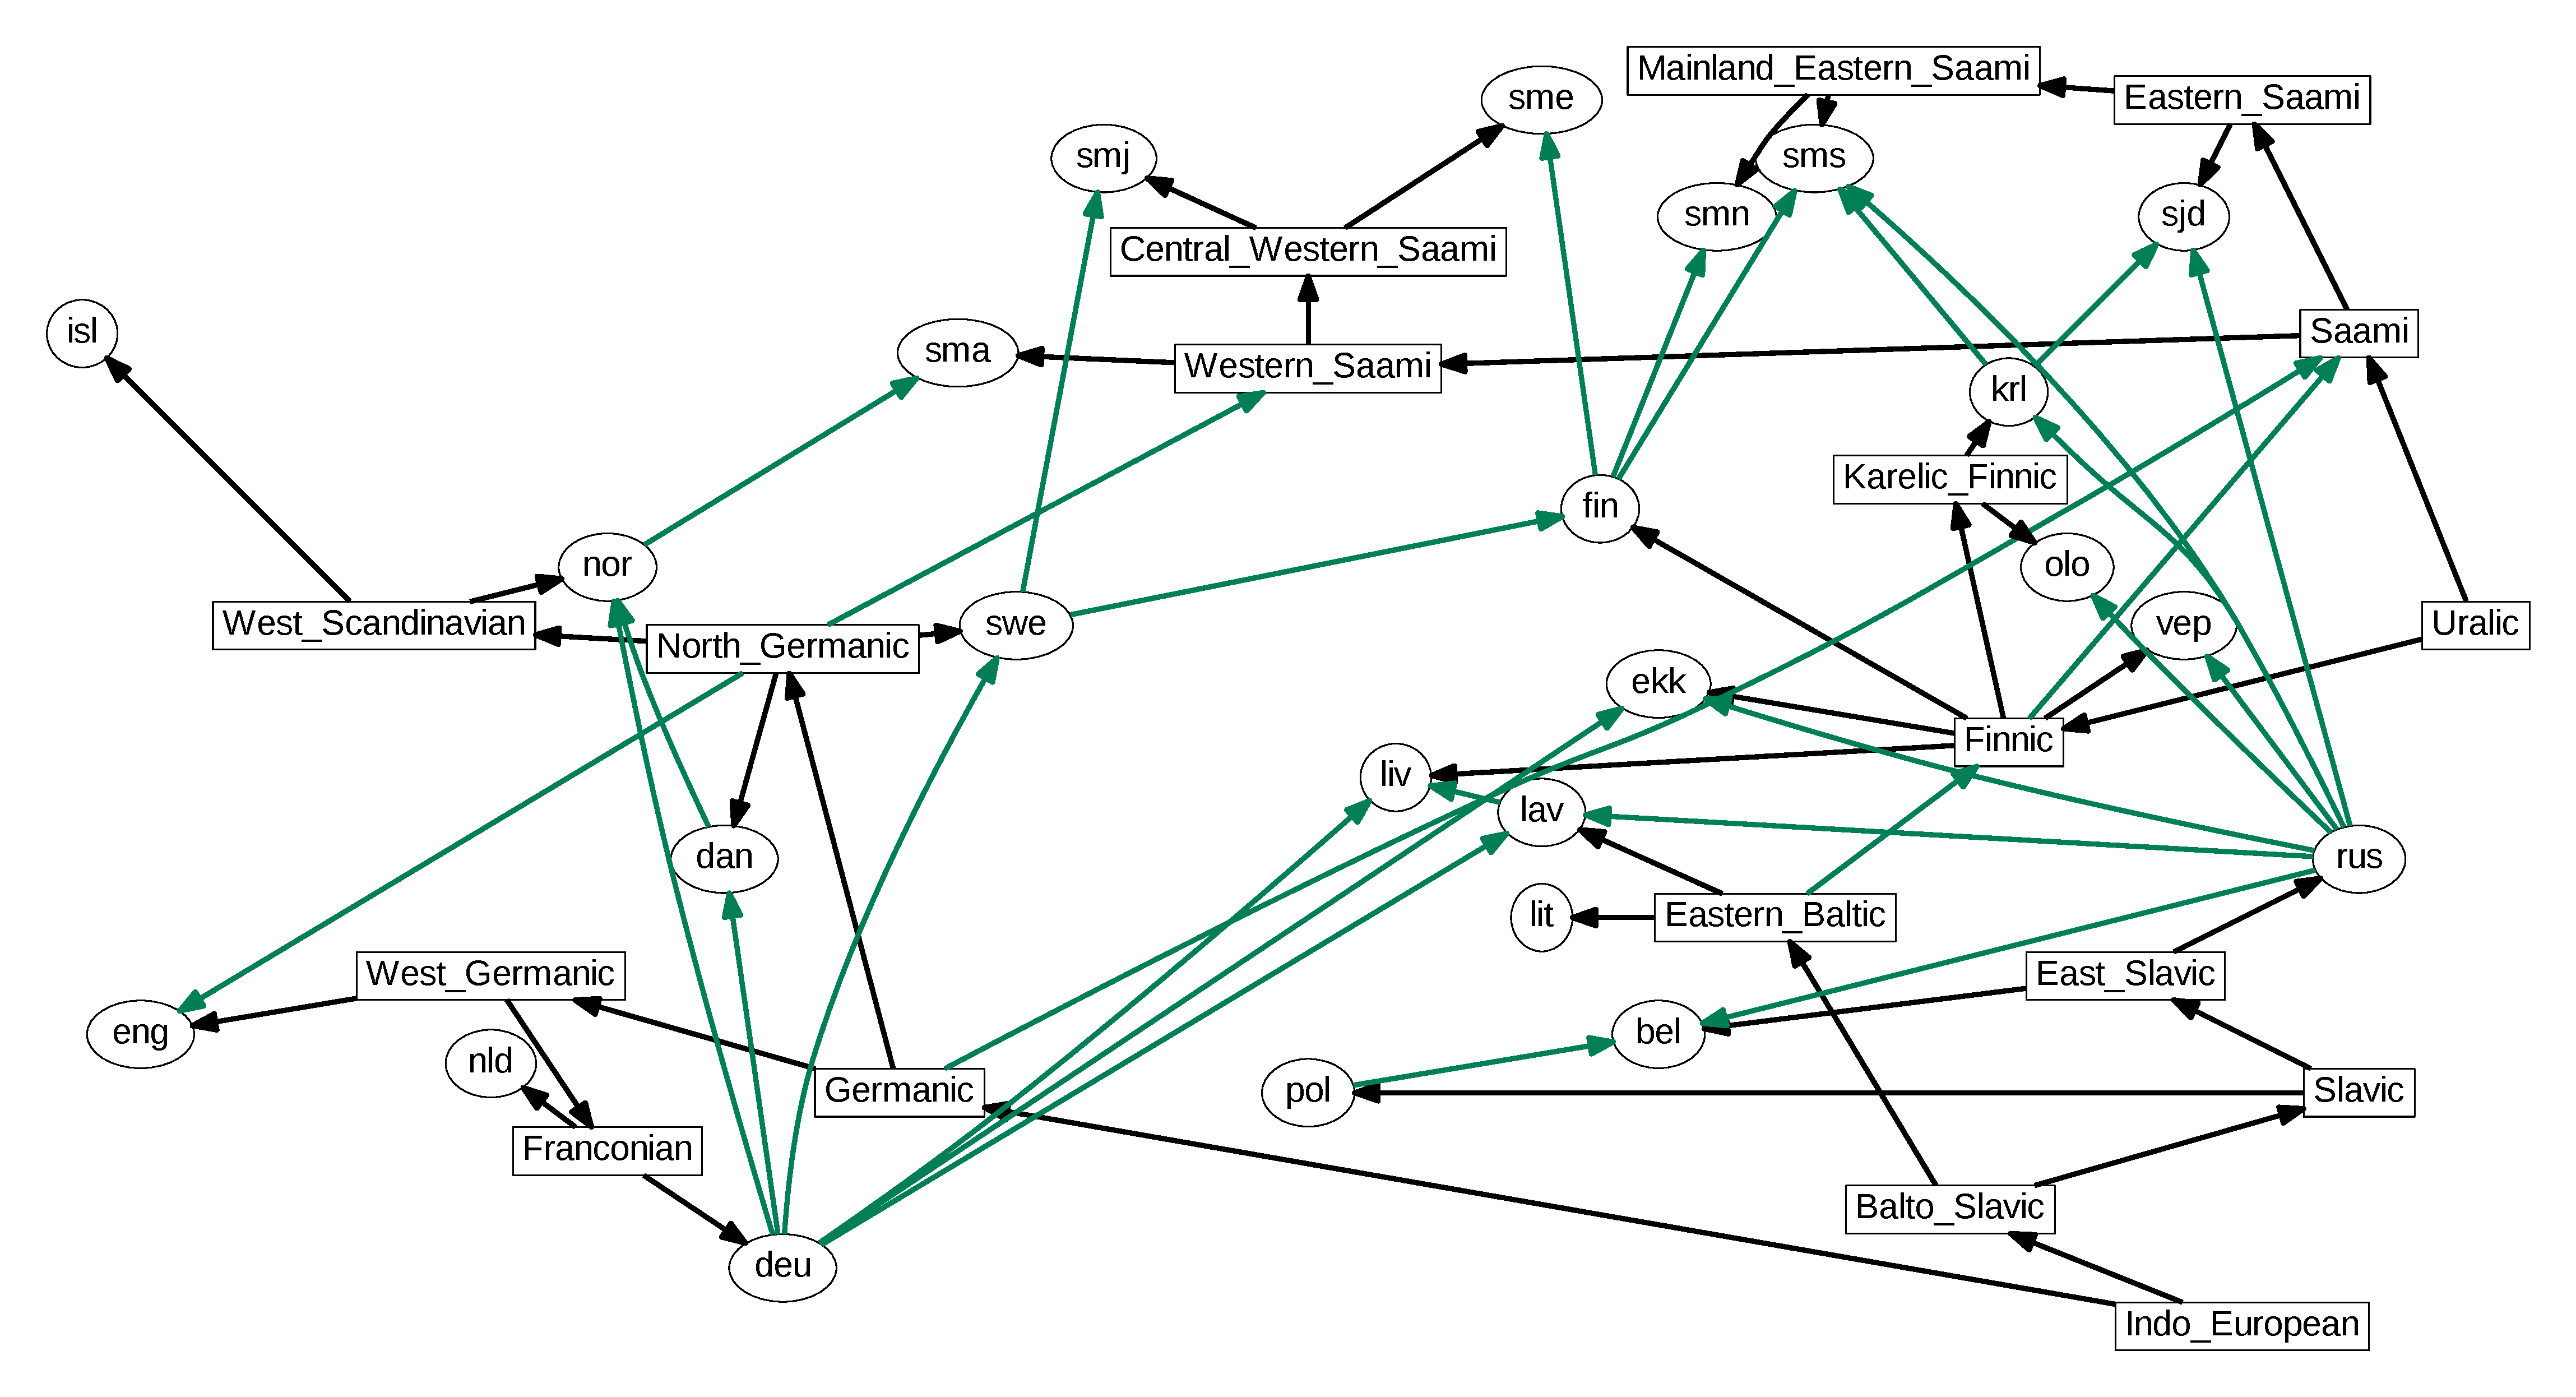
\includegraphics[width=\textwidth]{figures/goldstandard-phylo-baltic.pdf}
 \caption{Gold standard for phylogenetic flow on Baltic Sea data}
 \label{baltic-goldstandard-phylo}
\end{figure}

\subsection{Case study 2: Uralic and contact languages}
The second case study expands our horizon eastwards, to the point that it includes the Uralic languages with all their contact neighbors. This leads to a focus on European Russia, Scandinavia, and Western Siberia. Hungarian as a geographic outlier requires us to additionally include some further languages of Central and Eastern Europe, whereas the historical contacts of Uralic languages in Central Russia with Turkic neighbors leads us to also include some of the northern outliers of that family into the sample. We end up with a contact inference problem for a region stretching across 6,000 kilometers from west to east, and more than 3,000 kilometers from north to south, all of which is covered reasonably well by NorthEuraLex.

The Uralic language family\il{Uralic languages} consists of about 36 living languages (24 of which are covered by NorthEuraLex), which fall into nine firmly established branches. From west to east, these are Finnic, Saamic, Mordvinic, Mari, Permian, Hungarian, Mansi, Khanty, and Samoyedic. The highly divergent \ili{Samoyedic languages} are traditionally seen as forming the primary split within Uralic, with all the other branches being grouped together as Finno-Ugric\il{Finno-Ugric languages}. However, previously undetected cognates between Samoyedic languages and Eastern branches of Finno-Ugric have recently been discovered \citep{aikio2002,aikio2006etym}, which has considerably increased the number of reconstructable roots of Proto-Uralic, and contributed to a tendency to not necessarily assume this primary split to hold any longer. Moreover, a recent reanalysis of vowel correspondences \citep{hakkinen2007} has yielded some evidence that the primary split might have been between Finno-Permic\il{Finno-Permic languages} comprising the five western branches, and Ugro-Samoyedic on the other side, which then split into the four eastern branches. For the purposes of this work, the question of the internal structure of Uralic can be considered as open, and we will simply assume a comb-like structure formed by all the safely established branches.

The western branches Finnic and Saami were already described as part of the linguistic background for the first case study. Considering their relationship with the rest of Uralic, the Saami languages share so much lexical material with Finnic that these two branches have traditionally tended to be seen as forming a single Finno-Saamic\il{Finno-Saamic languages} phylogenetic unit. \cite{aikio2012} summarizes arguments for and against a closer affinity. The main problem is that the two branches do not show enough shared innovations in phonology to exclude ancient contacts as an explanation for their considerable lexical overlap. However, there still are some shared morphological innovations which are difficult to explain by contact alone.

The \ili{Mordvinic languages} (\textit{myv}, \textit{mdf}) and the \ili{Mari languages} (\textit{mhr}, \textit{mrj}), both of which could also be treated as dialect continua with two written standards each, have often been grouped together as the Volga-Fennic languages, but after a reassessment by \cite{bereczki1988}, this is now generally seen as a purely geographic grouping. Instead, as \cite{gruenthal2007} shows, if Mordvinic is considered part of a larger phylogenetic unit, it tends to be grouped together with Finnic and Saamic on lexical grounds.

Further to the east, the \ili{Permian languages} (\textit{kpv}, \textit{koi}, \textit{udm}) form the last branch of what some authors accept as the Finno-Permic branch of the Finno-Ugric languages. The Permian languages are closely related, with \ili{Udmurt} (\textit{udm}) in the Republic of Udmurtia being the most divergent. With more than 300,000 speakers, Udmurt is among the more viable minority languages of Russia. The other branch of Permic is formed by the highly divergent dialects of the Komi language, two of which are written languages. The 150,000 speakers of \ili{Komi-Zyrian} (\textit{kpv}) are distributed across a wide area in the northeastern part of European Russia. It is also one of the official languages in the Komi Republic, a very large territory covering much of the area west of the northern half of the Ural mountains. \ili{Komi-Permyak} (\textit{koi}), with little over 100,000 speakers, is the written standard for the Komi-Permyak Okrug in the Perm Krai, the Russian region south of the Komi Republic. The region around the Kama river where Udmurt and Komi-Permyak are spoken today is currently considered the most likely candidate for a Uralic urheimat \citep{hakkinen2009}, though alternative theories about a Siberian urheimat remain justifiable if one still assumes Samoyedic to form the primary split. Previous theories placing the homeland farther into Europe were based on archeological continuity arguments, and are now considered obsolete due to their lack of reliability \citep{hakkinen2006}.

In Western Siberia, the dialects of \ili{Khanty} (\textit{kca}) and \ili{Mansi} (\textit{mns}) have traditionally been grouped together as the \ili{Ob-Ugric languages}, but the close affinity is not accompanied by any shared innovations, and is therefore now seen by many uralists, like \cite{salminen2002}, as more likely due to intensive lexical contact (\textit{mns} \arrowOA \textit{kca} and \textit{kca} \arrowOA \textit{mns}). The \ili{Mansi} dialects are spoken by less than 1,000 people in the western parts of the Khanty-Mansi Autonomous Okrug, which covers a large part of the middle Ob and its tributaries east of the central Urals. \ili{Khanty} dialects are still spoken by almost 10,000 speakers in the eastern parts of the okrug, as well as neighboring areas to the north and east. \ili{Hungarian} (\textit{hun}) has been so much reshaped by its intensive contacts with other language families during the century-long migration of its speakers, that it now appears to form a branch of its own, although many 
isoglosses with the Ob-Ugric languages, particulary Mansi, do exist (such as the intensive use of verbal particles, highly unusual of Uralic), causing it to be placed next to the Ob-Ugric languages in all proposals of larger subunits. Lexically, the overlap with Khanty is stronger than that with Mansi, which is generally attributed to mutual contact (\textit{kca} \arrowOA \textit{hun} and \textit{hun} \arrowOA \textit{kca}).

Finally, the \isi{Samoyedic languages} (\textit{yrk}, \textit{enf}, \textit{sel}, \textit{nio}) form the easternmost branch of Uralic. The internal structure of this branch is not very clear. On lexical grounds, the southernmost surviving language Selkup (\textit{sel}) is clearly divergent from its northern relatives, but according to many other criteria, the Nganasan language (\textit{nio}) on the remote Taimyr peninsula is clearly the outlier. Perhaps due to its isolation, Nganasan is a very conservative language which shares some striking features (consonant gradation, vowel harmony) with the westernmost branch Finnic, hinting that these traits may have been present already at a very early stage of Uralic. By far the most viable of the Samoyedic languages is Nenets (\textit{yrk}), whose Tundra variant with more than 20,000 speakers is spoken in the far north on both sides of the Ural mountains. Closely related Enets, whose forest variant (\textit{enf}) is represented in NorthEuraLex, was once spoken along 
the entire lower Yenisei, but has been brought close to extinction under pressure of both Tundra Nenets and Russian. Selkup is still spoken by about 1,000 people in the region between Ob and Yenisei, and is the last surviving Southern Samoyedic language, which once also included the now extinct Kamassian and Mator languages of the Sayan mountains west of Lake Baikal.

While the contacts between Western Uralic and Germanic or Baltic languages in the Baltic sea region were already described in the preceding section, the complex contact history of \isi{Hungarian} (or Magyar) warrants some more detailed remarks. During their long migration from the Ural region (where the closest relatives Khanty and Mansi still reside) to central Europe, a process which most probably took about 2,000 years, \ili{Hungarian} first had intensive contact with the \ili{Permian languages} (\textit{hun} \arrowOA {Permian} or \textit{Permian} \arrowOA {hun}). Leaving the area of Uralic speakers on their way to the southwest, Hungarians next encountered and were influenced by Iranian\il{Iranian languages} tribes (\textit{Iranian \arrowLA hun}), and later ended up under G\"okt\"urk rule on the Black Sea, where Western \ili{Turkic languages} became the source of a lot of cultural vocabulary (\textit{Turkic \arrowLA hun}). After the collapse of the Khazar empire, the Hungarians then undertook their final migration westward, conquering and settling in the Carpathian Basin at the end of the ninth century. Here, they acquired further strata of loans from both West Slavic\il{West Slavic languages} and South Slavic\il{South Slavic languages} (\textit{West Slavic, South Slavic \arrowLA hun}), especially in the semantic fields of agriculture and household items. \ili{German} influence is especially visible in the fields of military and engineering, whereas \ili{Latin} provided the words for many religious and philosophical concepts. While the rapidly expanding Kingdom of Hungary had Latin as its official language well into the 19th century, limiting the influence of Hungarian on the Slavic minorities, Hungarian language policy during the late stages of the Austro-Hungarian empire developed a strong tendency towards Magyarization. This led to Hungarian influence especially on \ili{Croatian} and \ili{Slovak}, although this is barely visible in the basic vocabulary. The same is true for \ili{Turkish} influence during the period of Ottoman rule in the 16th and 17th centuries.

The other major historical influence on Uralic languages is caused by the direct neighborhood of the Volga-Fennic and southern Permian languages with the Turkic languages \ili{Chuvash} (\textit{chv}), \ili{Tatar} (\textit{tat}), and \ili{Bashkir} (\textit{bak}). In the case of the \ili{Mari languages}, the influences of neighboring Chuvash (\textit{chv \arrowLA Mari}) and Tatar (\textit{tat \arrowLA Mari}) is the strongest. Among \ili{Permian languages}, \ili{Udmurt} has become most influenced by its Turkic southern neighbors Tatar (\textit{tat \arrowLA udm}) and Bashkir (\textit{bak \arrowLA udm}). These contacts, including layers of loans which have not had much influence on the basic vocabulary, are described extensively by \cite{rona-tas1988}.

After the initial splits, there has been some limited contact between neighboring branches of Uralic. According to \cite{hausenberg1998}, Komi merchants caused \ili{Komi-Zyrian} to become an influential trade language of the north, with some influence on \ili{Nenets} (\textit{kpv} \arrowOA \textit{yrk}) and \ili{Mansi} (\textit{kpv} \arrowOA \textit{mns}), which is however only barely visible in the basic vocabulary of these languages. In the east, \ili{Khanty} and \ili{Selkup} have interacted quite intensively (\textit{kca} \arrowOA \textit{sel}), and \ili{Enets} was heavily influenced through mixed marriages with the closely related and much more vital Nenets community (\textit{yrk} \arrowOA \textit{enf}) before its few remaining speakers started shifting towards \ili{Russian} \citep{siegl2013}.

The pervasive development in all the Uralic minority languages, however, is a shift towards \ili{Russian} as the language of school and the workplace. While some of these languages still have hundreds of thousands of speakers, in all cases the speaker communities are dominated by the old people in rural areas, whereas city life as well as mass culture and all modern economic activity takes place exclusively in Russian. This very strong tendency puts the future of all the Uralic minority languages very much into question, even more so as the current political climate tends to be hostile to any activities which can be interpreted as fostering separatist tendencies within Russia \citep{taagepera2013}.

But Russian influence does of course reach back much farther than the introduction of a comprehensive school system by the Soviets. Russian influence on the lexicon is observable in all minority languages, but some languages (\ili{Kildin Saami}, \ili{Erzya}, \ili{Hill Mari}, \ili{Udmurt}, \ili{Komi}) show more Russian influence even in basic vocabulary than others which tend to be more purist at least in their written variants (\ili{Moksha}, \ili{Meadow Mari}). The following contacts are reflected so strongly in the basic vocabulary that they were added to the gold standard: \textit{rus} \arrowLA \textit{olo, vep, sjd, sms, myv, mrj, udm, koi, kpv, kca, mns, yrk, sel, enf, nio}.

Among the languages which are included in this case study chiefly by virtue of having been in contact with \ili{Hungarian}, \ili{Romanian} is a Romance language whose lexicon was heavily influenced by surrounding \ili{Slavic languages} (\textit{Slavic} \arrowOA \textit{ron}). According to \cite{schulte2009}, there are also traces of \ili{German} (\textit{deu} \arrowOA \textit{ron}) and Hungarian (\textit{hun} \arrowLA \textit{ron}) loans in the basic vocabulary. Outside the scope of this case study, Romanian also contains a layer of ancient loans from \ili{Albanian} or a closely related language (\textit{sqi} \arrowOA \textit{ron}), many loanwords from written \ili{Latin} (\textit{lat} \arrowOA \textit{ron}) as well as some from \ili{Greek} (\textit{ell} \arrowOA \textit{ron}). A substantial number of later loans came from \ili{Turkish} (\textit{tur} \arrowLA \textit{ron}), and the words for many concepts of modern life were borrowed from \ili{French} (\textit{fra} \arrowOA \textit{ron}).

\figref{uralic-cognacy} visualizes the cognacy overlaps between the \ili{Uralic languages} and their neighbors. The rather chaotic picture already indicates that this case study is more of a challenge for lexical flow detection than the Baltic Sea study. The highest overlaps cluster the Western Uralic languages (Finnic and Saami) together. Also, the Germanic\il{Germanic languages} and \ili{Slavic languages}, the two Baltic languages as well as the four \ili{Turkic languages} clearly appear as clusters. The central and eastern branches of Uralic are clearly least distinctive, mirroring the unclear second-level structure of the family. \ili{Hungarian} has overlaps of medium strength with many Uralic languages as well as Slavic neighbors, making it a major challenge to detect its affinity with the \ili{Ob-Ugric languages}.

\begin{sidewaysfigure}
 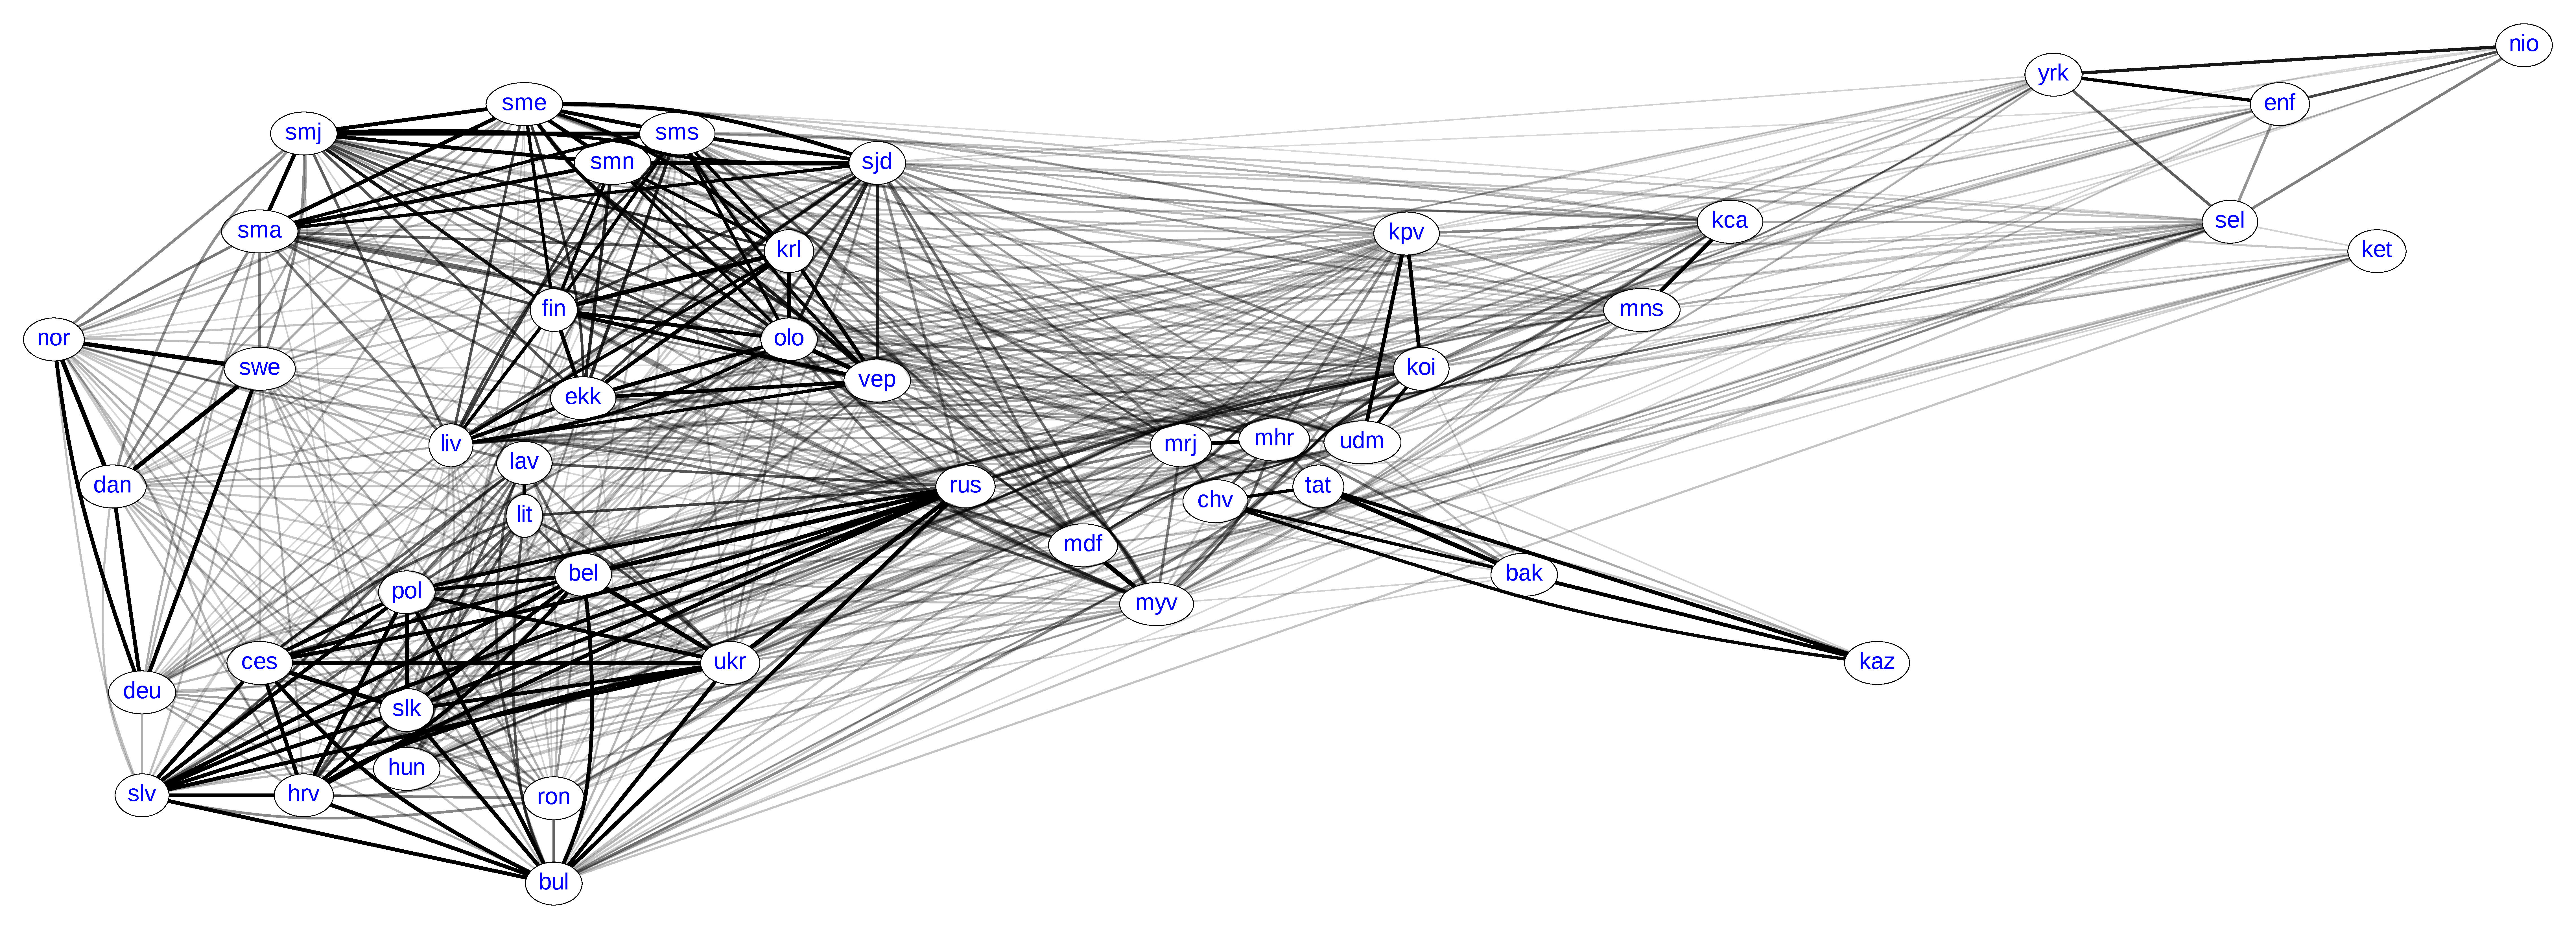
\includegraphics[width=\textwidth]{figures/cognacy-strength-uralic.pdf}
 \caption{Visualization of inferred cognate overlap in the Uralic data}
 \label{uralic-cognacy}
\end{sidewaysfigure}

\figref{uralic-goldstandard-phylo} visualizes the ideal result of phylogenetic flow inference. Note that some of the connections of \ili{Hungarian} are light green lines, indicating that the direction of influence is unclear, which makes an undirected arc in an automatically inferred network just as acceptable as an arrow in either direction.

\begin{sidewaysfigure}
 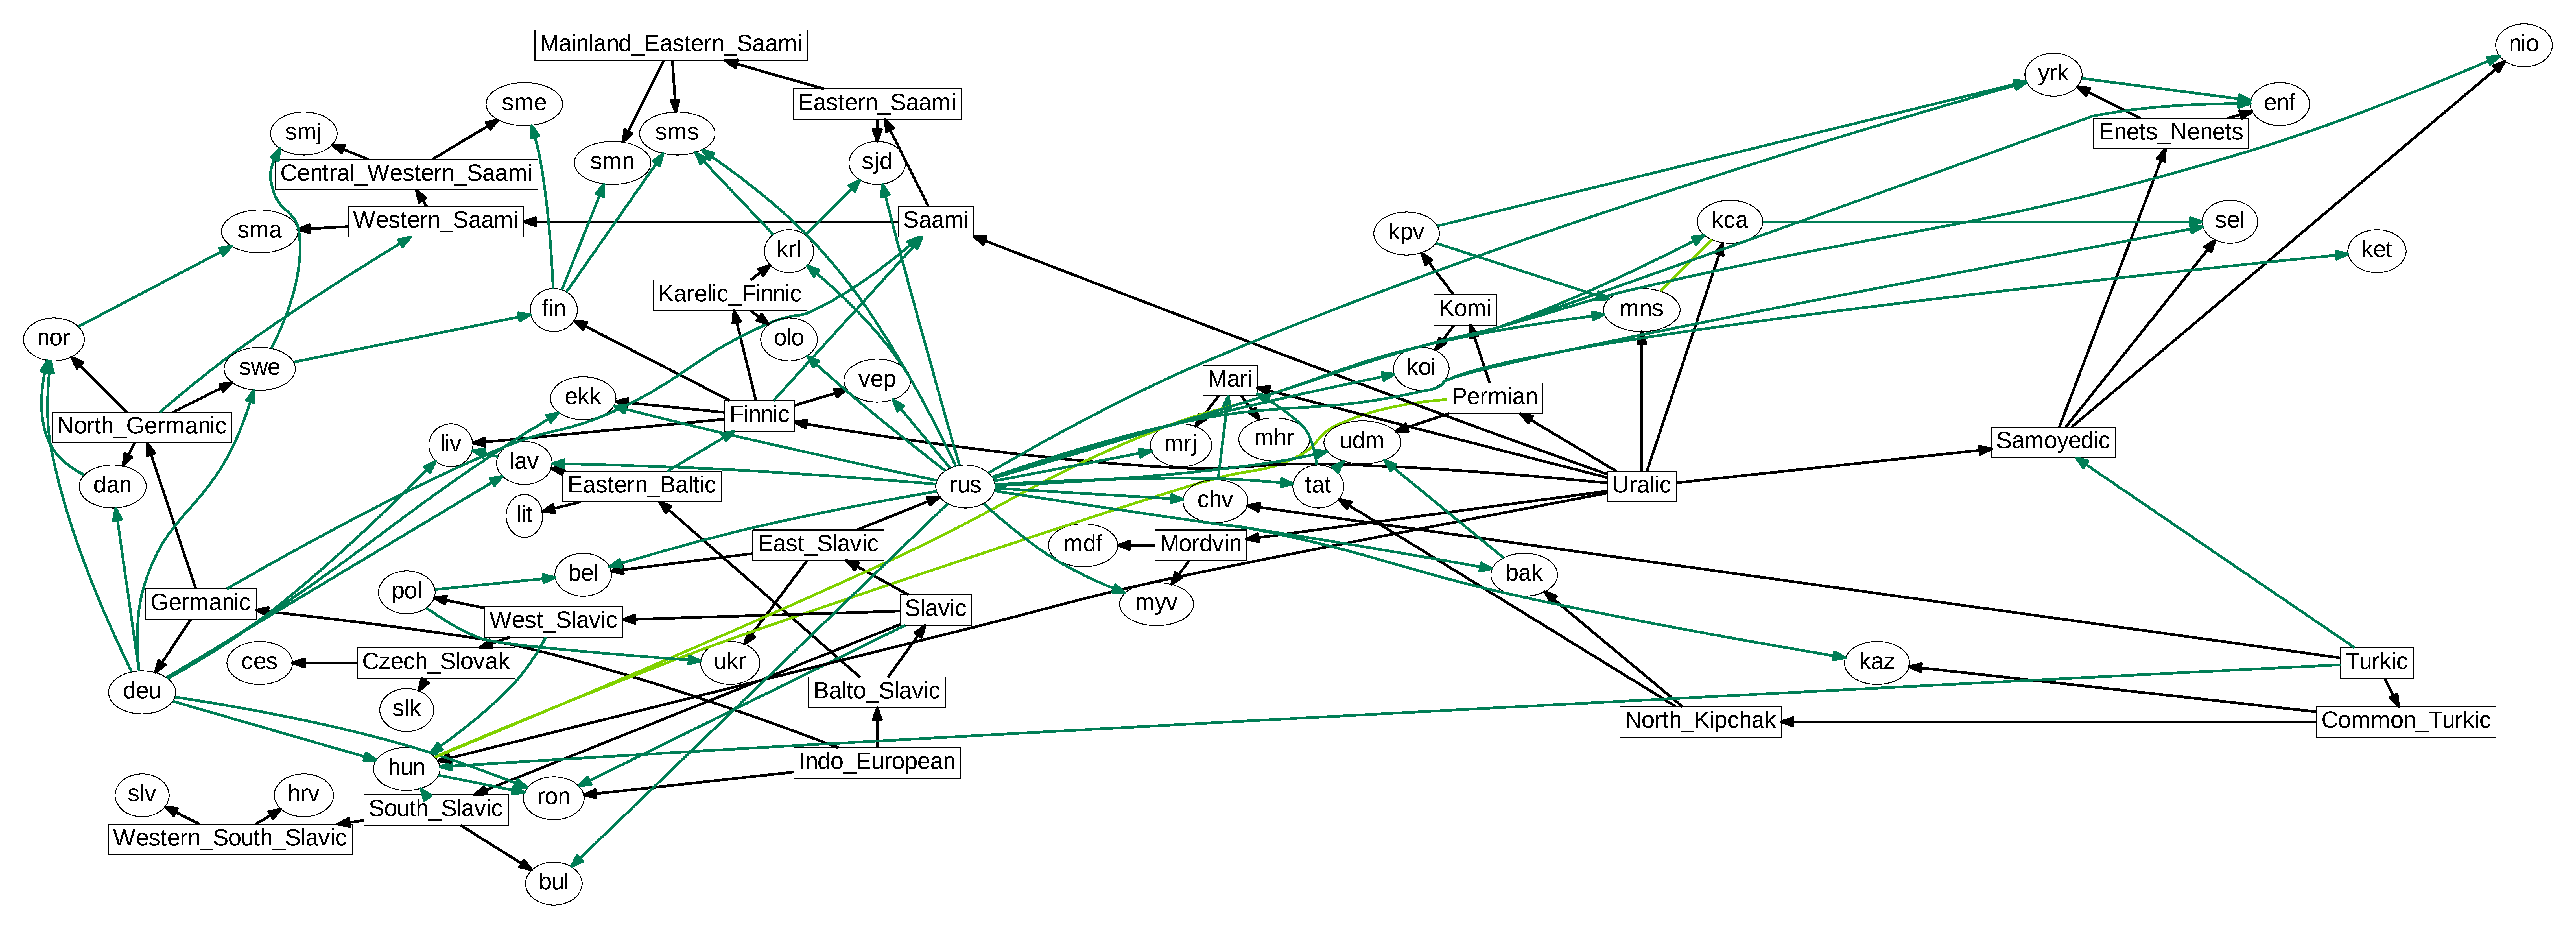
\includegraphics[width=\textwidth]{figures/goldstandard-phylo-uralic.pdf}
 \caption{Gold standard for phylogenetic flow on Uralic data}
 \label{uralic-goldstandard-phylo}
\end{sidewaysfigure}

\subsection{Case study 3: the linguistic landscape of Siberia}
The next case study deals with inferring contacts between the languages of Siberia. Siberia is a sparsely populated region where many ancient language families were able to survive until today, although all of the oldest languages have become small minority languages on the verge of disappearing. The number of language families in this test set is much larger than in the previous ones, and the high number of isolates generates additional challenges to lexical flow inference.

The dominant influence of the colonial language \ili{Russian} is of course visible in every minority language of Siberia. Some languages show less influence in the basic vocabulary than others, however. For instance, \ili{Itelmen} has borrowed extensively from Russian even in its basic vocabulary, whereas pressure on related \ili{Chukchi} was noticeably lower, most likely due to much later colonization (early 18th vs. early 20th century). While Russian has borrowed some words from \ili{Turkic languages}, this has not left measurable traces in the basic vocabulary, and borrowings from other Siberian languages only occur in specialized areas of local significance, such as reindeer herding, tent styles, and animal and plant names.

In western Siberia, the eastern branches of Uralic\il{Uralic languages} (\textit{mns, kca, sel, yrk, enf, nio}) have interacted with each other as well as Siberian languages to varying degrees. The influences of Khanty on Selkup (\textit{kca} \arrowOA \textit{sel}) and of Nenets on Enets (\textit{yrk} \arrowOA \textit{enf}) were already discussed, as were the western contacts of the Ket language. Concerning influences on Uralic from the east, Samoyedic\il{Samoyedic languages} has borrowed a few dozen words from Early Turkic\il{Turkic languages} (\textit{Turkic \arrowLA Samoyedic}), which are summarized by \cite{dybo2007}. Also, \cite{anikin_helimski_2007} list substantial numbers of loans from Tungusic\il{Tungusic languages} into Samoyedic (\textit{Tungusic} \arrowLA \textit{Samoyedic}).

All three language families (Turkic, Mongolic, and Tungusic) which are subsumed as Core Altaic\il{Altaic languages} by advocates of a deep relationship, play major roles in the linguistic landscape of Siberia. While the exact relationship between these three well-established families (whose typological similarities are indeed quite striking) is an eternal bone of contention, it is clear that even if there were no ancestral relationship, the three proto-languages must have been in very intensive and long-lasting contact with each other. During recorded history, the \ili{Turkic languages} have formed the westernmost of the three families (starting out in the Altai region), the \ili{Mongolic languages} have been in the center (Mongolia and adjacent areas), and the Tungusic\il{Tungusic languages} tribes originally settled in the east (Manchuria). The contemporary distribution pattern still shows this general tendency, but has been complicated by many migrations of these highly mobile nomadic peoples. For 
instance, the westernmost Mongolic language \ili{Kalmyk} (\textit{xal}) is spoken in Kalmykia, a republic in European Russia, whereas the easternmost Turkic language \ili{Sakha} (\textit{sah}) is spoken in the Sakha republic (also called Yakutia) which covers a large part of Eastern Siberia. Tungusic peoples have spread throughout Siberia, with the westernmost speakers of \ili{Evenki} (\textit{evn}) neighboring the Kets\il{Ket} on the Yenisei, and the \ili{Manchu} (\textit{mnc}) in the south at one point conquering China and becoming the ruling elite of Qing, the last imperial dynasty of China.

\ili{Turkic languages} (\textit{tur}, \textit{azj}, \textit{tat}, \textit{bak}, \textit{kaz}, \textit{uzn}, \textit{sah}, \textit{chv}) are present throughout Russia, the Caucasus, Central Asia, Northern Iran, and Turkey. The following summary is based on the handbook of Turkic languages edited by \cite{johanson_csato_1998}, with some additional information from \cite{menges1995}. In genealogical terms, the Oghur subbranch\il{Oghur Turkic languages}, to which the \ili{Chuvash} language (\textit{chv}) of European Russia belongs, is a clear outlier, with at least 2,000 years of separate development, which puts the date of the latest stage of Proto-Turkic at about 500 BC. The Chuvash language is closely related to the extinct languages of the Bulgars and Khazars, and some scholars consider it likely that the \ili{Hunnic} language was Oghur Turkic as well.

The rest of Turkic, also called \ili{Common Turkic}, forms a much closer genealogical unit,
which probably still formed a single dialect continuum in 550 AD, when the Turkic expansion set in. This is also the date of the first written records in a Turkic language, the Orkhon inscriptions of the G\"okt\"urk khaganate. During the Turkic expansion in the 6th-11th centuries, Common Turkic separated into five branches, four of which are represented in NorthEuraLex.

The major \ili{Oghuz Turkic languages} are \ili{Turkish} (\textit{tur}), \ili{Azeri} or Azerbaijani (\textit{azj}), and \ili{Turkmen}. The Oghuz tribes arrived in Central Asia during the 8th century, formed a new warrior elite governing older Iranian states, and then started to spread to the southwest in the 11th century, founding the Seljuk Empire and invading Anatolia, where they later formed the Ottoman Empire and modern Turkey.

The Kipchak tribes\il{Kipchak Turkic languages} spread to the northwest, their farthest outliers in the Ural region mixing with the local population and separating into \ili{Bashkir} (\textit{bak}) and \ili{Tatar} (\textit{tat}), whose contacts we already discussed when covering Uralic and its neighbors. Most Turkic languages of the North Caucasus belong to the Cuman branch of Kipchak, others to the Nogai branch, which also includes the \ili{Kazakh} (\textit{kaz}) language. Finally, \ili{Kyrgyz} and some related smaller languages form another branch of Kipchak.

The Karluk tribes\il{Karluk Turkic languages} migrated to the southeast, came into intensive contact with Islam, and played a big role in the politics of China, before becoming the ruling class of the Timurid empire. The Karluks later gave rise to the modern \ili{Uzbek} (\textit{uzn}) and \ili{Uyghur} ethnicities.

The final direction, the northeast, led some Turkic tribes into Siberia\il{Siberian Turkic languages}, where most (such as the Tuvans and Chulyms) stayed near the Altai mountains, whereas one tribe migrated far to the north and became the Sakha or Yakuts, now the titular nation of the Russian federal subject which is largest in area, the Sakha Republic, which covers more than 3 million square kilometers, and where the \ili{Sakha} language (\textit{sah}) is still spoken by 400,000 people, about 40\% of the population.

The final branch of Common Turkic, Arghu\il{Arghu Turkic languages}, only consists of \ili{Khaladj}, a minority language of 40,000 speakers in central Iran, which lets it fall outside the scope of a comprehensive lexical database of Northern Eurasia.

Only two of the Turkic languages in NorthEuraLex, \ili{Kazakh} and Sakha, are relevant for the Siberian case study. Spread across the steppe zone directly to the south of Western Siberia, the Kazakhs were in intensive contact with Mongolian tribes, and borrowed many words for military and administrative terms from them (\textit{Mongolic} \arrowLA \textit{kaz}). \ili{Sakha} (\textit{sah}) is the only Siberian Turkic language currently represented in NorthEuraLex, but by far the one which has had most influence on the linguistic history of Siberia. Sakha contains some lexical material borrowed from its Mongolic\il{Mongolic languages} southern neighbors (\textit{bua}, \textit{xal} \arrowLA \textit{sah}), whereas a lot of the vocabulary of modern life was taken over from \ili{Russian} (\textit{rus} \arrowLA \textit{sah}).

The \ili{Mongolic languages} (\textit{khk}, \textit{bua}, \textit{xal}) are concentrated in Mongolia and neighboring regions of Russia and China. A very comprehensive overview of the family is given by \cite{janhunen2003}, which is also my main source about Mongolic languages. As a language family, the time depth of Mongolic is not very high, as all the living and attested languages are descended from dialects of \ili{Middle Mongol}, the language of the Mongol Empire in the 13th century. The most divergent Mongolic language, the probably now extinct \ili{Moghol} language of Afghanistan, is actually a remnant of one of Genghis Khan's armies which was stationed there during those times. The other outlier is the \ili{Daur} language of Inner Mongolia and neighboring provinces of China, which is already very close (50\% lexical overlap) to \ili{Khalkha Mongolian}. The remainder of the language family is split into two dialect continua. Southern Mongolic contains several minority languages of Northern China, some of them (\ili{Mongguor}, \ili{Dongxiang}) with hundreds of thousands of speakers, whereas the larger dialect cluster, Central Mongolic, which covers the northern half of the language family's area, subsumes about 80\% of all speakers of Mongolic languages. Since documentation of all smaller Mongolic languages exists mostly in Chinese and is difficult to come by, NorthEuraLex currently only contains three variants of Central Mongolian, with very different and interesting contact histories.

\ili{Khalkha Mongolian}\il{Mongolian} (\textit{khk}), the national language of the Republic of Mongolia, is by far the most stable of all Mongolic languages, partly at the cost of other Central Mongolian languages which only count as dialects of the national language. While being rather purist in recent times, Khalkha Mongolian has small layers of loanwords from \ili{Old Turkic} (\textit{Turkic} \arrowLA \textit{khk}), \ili{Sanskrit}, \ili{Persian}, \ili{Arabic}, Tungusic, and Chinese, most of which do not involve the most basic vocabulary, and a large layer of recent \ili{Russian} loans (\textit{rus} \arrowLA \textit{khk}) for scientific and technical vocabulary. Dialects subsumed under the name \ili{Buryat} (\textit{bua}) are spoken in Southern Siberia, Eastern Mongolia, and adjacent areas of China. The variant included in NorthEuraLex is based on Russian sources, and therefore includes many loanwords from Russian (\textit{rus} \arrowLA \textit{bua}). The Buryats, the most populous indigenous nation of Siberia at the beginning of Russian conquest, have exerted considerable cultural influence on many of the neighboring peoples, especially \ili{Sakha} and the \ili{Tungusic languages}. \ili{Kalmyk} (\textit{xal}) is a written variant of \ili{Oirat}, a group of Mongolic dialects of limited mutual intelligibility with Khalkha whose 360,000 speakers are spread throughout the westernmost parts of Mongolia, Xinjiang, Kyrgyzstan, and Kalmykia on the lower Volga. During their expansion, the Oirats often formed federations with Kipchak\il{Kipchak Turkic languages} tribes, from whom they borrowed quite a bit of cultural vocabulary (\textit{Kipchak} \arrowLA \textit{xal}). The remaining Oirat communities seem to be in the process of losing their ancestral language, and even the official language of Kalmykia, with some 80,000 speakers left, is only spoken fluently by the elderly, ever since the transmission of Kalmyk culture to the younger generations was interrupted by Stalin's deportations, which led to the demise of a substantial part of the Kalmyk population, and left heavy traces on their language (\textit{rus} \arrowLA \textit{xal}).

The \ili{Tungusic languages} (\textit{evn}, \textit{gld}, \textit{mnc}), though covering a very large geographical area, are thinly dispersed and under threat. A compact overview of the Tungusic languages and their current situation is given by \cite{janhunen2005}. \ili{Xibo}, the largest surviving Tungusic language by number of speakers, and one of only two languages which are still learnt by children, is spoken by the descendants of a single tribe which was deployed to the border by the Qing government. Due to a lack of accessible resources on Xibo, the closely related and well-documented \ili{Manchu} language (\textit{mnc}), the national language of the Qing dynasty, which now only has a handful of elderly speakers left, was chosen to represent this branch of Tungusic. The Manchu of the written sources contains many loanwords from Chinese (\textit{cmn \arrowLA mnc}) and Mongolian (\textit{khk \arrowLA mnc}).

The second branch of Southern Tungusic is dominated by \ili{Nanai} (\textit{gld}), still spoken by about 1,400 speakers, less than 10\% of ethnic Nanai on both sides of the Chinese-Russian border. The core of the language community is formed by three almost exclusively Nanai villages in the Khabarovsk Krai. Like most other minority languages, it remains in daily use only among elderly speakers, whereas the younger generations have switched to Russian. The Nanai language has borrowed from \ili{Chinese} and from \ili{Russian} (\textit{cmn, rus \arrowLA gld}), but also shares some lexical items with \ili{Mongolic languages}, probably due to borrowing (\textit{bua \arrowLA gld}), since the shared vocabulary contains items beyond those reconstructed even by advocates of common inheritance.

While \ili{Evenki} (\textit{evn}), the largest Northern Tungusic language, still has some 30,000 speakers, due to its very wide geographical dispersal across much of Eastern Siberia and Manchuria it has split into many very divergent dialects, and its speakers tend to live in mixed-language settlements where they almost always form a minority. For this reason, Evenki speakers in Siberia today tend to not only prefer Russian for communication, but are often able to communicate with their non-Russian neighbors (Sakha, Buryat) in their respective languages. The Evenki lexicon, depending on the dialect, contains strong influences from \ili{Russian} (\textit{rus  \arrowLA evn}), \ili{Sakha} (\textit{sah \arrowLA evn}), and \ili{Buryat} (\textit{bua  \arrowLA evn}).

The oldest language families still present in Siberia (all of which now marginalized and severely endangered) are grouped together as the \ili{Paleosiberian languages}, a convenience term without any grounding in phylogeny. From a comparative point of view, they can be split into not fewer than five small language families and isolates. From northwest to southeast, these families are Yeniseian, Yukaghir, Chukotko-Kamchatkan, Nivkh, and Ainu.

In central Siberia, the \ili{Ket} language (\textit{ket}) is the last surviving Yeniseian language\il{Yeniseian languages}, whose relatives were once spoken along most of the river Yenisei. Ket is typologically vastly different from all other Siberian languages, in being a tonal as well as a predominantly prefixing language, and featuring an extremely complex verbal morphology that is more similar in structure to many North American languages than to anything in the Old World (except perhaps Northwest Caucasian\il{Northwest Caucasian languages}). According to \cite{vajda2009}, before the relatively recent and limited influence of \ili{Russian} (\textit{rus} \arrowLA \textit{ket}), which set in so late that it mostly resulted in language shift, there were contacts with the Samoyeds to the east (predominantly the Selkups\il{Selkup}, from which the Ket took the reindeer terminology), the \ili{Evenki} to the east, and to a much smaller extent with Turkic tribes to the south. However, most of these contacts were hostile, and only led to a bare minimum of lexical material being transferred. Among the NorthEuraLex languages contained in the WOLD, Ket is the language with the lowest overall borrowing rate, at 9.7\% of the investigated part of the lexicon. This reflects the fact that, as Vajda explains, the Ket culture with their hunter-gatherer economy only managed to survive in central Siberia until today because the mosquito-infested marshlands make it impossible to keep even reindeer in the upper Yenisei region, making their homeland entirely unattractive for conquest and colonization. This limited the intensity of language contacts until Soviet times, when collectivization and the boarding school system caused the traditional lifestyle to disappear, and the dominance of Russian as the school language caused the number of Ket speakers to dwindle, with as little as 100 speakers left in 2008.

Much further to the east, we can find the last remnants of the Yukaghir language\il{Yukaghir languages} family (\textit{ykg}, \textit{yux}) which in precolonial times still covered a large area between the Lena and Anadyr rivers, but is now reduced to two isolated pockets of a few dozen elderly speakers on the eastern border of the Sakha republic. The more northerly of the two surviving varieties, \ili{Tundra Yukaghir} (\textit{ykg}), is reasonably well-documented, whereas \ili{Kolyma Yukaghir} (\textit{yux}), forming the southern end of an ancient dialect continuum and not mutually intelligible with the Tundra variant, has only recently seen systematic documentation efforts, culminating in the first full grammar by \cite{maslova2003}. Reconstructed Proto-Yukaghir shows some overlap in basic vocabulary with \ili{Uralic languages}, which is predominantly taken as a very early loanword layer from Proto-Uralic (or a predecessor spoken in Siberia). According to an analysis by \cite{hakkinen2012}, this layer of 
about 50 loanwords can be separated into an older (Pre-Proto-Uralic) and a younger (Proto-Uralic) layer. For simplicity, and because I will not be attempting to move beyond established families, these early contacts are reflected by a single arrow $Uralic \rightarrow Yukaghir$ in the gold standard. In the less basic vocabulary, an additional layer of about 30 later loans from Samoyedic\il{Samoyedic languages} increases the impression of deep affinity, but is not visible in the NorthEuraLex data. The Yukaghirs are suspected to have been the original inhabitants of an even larger area, which were then gradually displaced by three consecutive waves of migration. The Tungusic peoples were the first to introduce reindeer as mounts and pack animals into the region, allowing them to hunt more efficiently, and forcing the Yukaghir hunter-gatherers further to the north (\textit{evn} \arrowLA \textit{Yukaghir}). As described by \cite[p. 52]{menges1995}, the Turkic \ili{Sakha} people were the next to move northward, 
introducing horses, metalworking and a limited form of agriculture to what is now the Sakha republic (\textit{sah} \arrowLA \textit{Yukaghir}). Easily taking control of the few attractive pastures, they marginalized the sparse \ili{Evenki} population, who in turn took additional territory from the Yukaghirs, forcing them to evade even further to the northeast. Finally, \cite{viires_vahtre_1993} describe how Russian colonization (\textit{rus} \arrowLA \textit{ykg}, \textit{yux}) with tribute demands, hostage taking and the spread of diseases, drastically worsened the living conditions for all native peoples, bringing the already marginalized Yukaghirs close to extinction. The younger generations of surviving ethnic Yukaghirs have shifted completely to \ili{Russian} and/or Sakha.

The largest Paleosiberian language family is Chukotko-Kamchatkan\il{Chukotko-Kamchatkan languages} (\textit{ckt}, \textit{itl}), whose speakers form the indigenous population of easternmost Siberia, from Chukotka in the extreme northeast to the Kamchatka peninsula in the south. Being polysynthetic languages, they are typologically similar (but not provably related) to neighboring Eskimo-Aleut\il{Eskimo-Aleut languages}. The Kamchatkan branch of the family consists of the single moribund language \ili{Itelmen} (\textit{itl}), and diverges a lot from the northern branch Chukotkan, which consists of \ili{Chukchi} (\textit{ckt}) and three further languages which are so similar to Chukchi that they could be considered dialects of a single language. While severely endangered like all Paleosiberian languages, Chukchi with almost 7,000 speakers has by far the highest chances of survival, although according to \cite{dunn2000}, the newly created written standard variant is at odds with some important cultural 
traditions, with negative impacts on the language's viability. The Chukotko-Kamchatkan languages show some ancient lexical influences from Eskimo-Aleut (\textit{Eskimo-Aleut} \arrowLA \textit{Chukotko-Kamchatkan}), and also some from Yukaghir\il{Yukaghir languages}, although the latter largely concern reindeer herding and climate-specific terminology, and both are barely visible in the basic vocabulary \citep{volodin_skorik_1997}. \ili{Russian} influence has only recently become dominant due to mixed marriages and its pervasive role in economic life, after the Chukchis had successfully resisted colonization during the centuries before. In contrast, \ili{Itelmen} has been under massive Russian influence for several generations (\textit{rus} \arrowLA \textit{itl}), and has even borrowed many functional elements in a situation of complete bilingualism \citep{viires_vahtre_1993}.

The \ili{Nivkh} language (\textit{niv}) was once spoken across the Lower Amur and Northern Sakhalin, and is still spoken by about 200 elderly people distributed across dozens of villages in the area. The language of this people of fishermen and hunters shows some typological similarities with Chukotko-Kamchatkan\il{Chukotko-Kamchatkan languages}, and some overlap in basic vocabulary with all of the neighboring languages, but too little to show regular sound correspondences, leaving conservative scholars no choice but to classify the language as an isolate. An overview of the language is given by \cite{gruzdeva1998}. Throughout their history (which does not seem to have involved any migrations for thousands of years), the Nivkhs were influenced culturally by neighboring Tungus peoples, especially the \ili{Nanai} (\textit{gld \arrowLA niv}). Some lexical overlap with the neighouring \ili{Ainu} dialects can be observed as well, hinting at intensive ancient contacts, but it is not always clear in which direction 
the words were borrowed. All the words for concepts which are not immediately relevant to the traditional lifestyle, including everything concerning agriculture, were only recently borrowed from \ili{Russian} (\textit{rus} \arrowLA \textit{niv}), which has completely replaced the ancient language in the younger generations, although the size of the ethnic population has remained stable at about 5,000 people since the beginning of colonization.

The \ili{Ainu} (\textit{ain}) language of Hokkaido and historically Sakhalin is another isolate which is sometimes counted as a Paleosiberian language. Descending from an indigenous population which probably once settled much of northern Japan, only the Hokkaido dialect has barely survived into our time, with fewer than ten elderly speakers remaining. Ainu shows some lexical overlap with its northern neighbor \ili{Nivkh} (probably \textit{ain} \arrowLA \textit{niv}), and has borrowed massively from \ili{Japanese} (\textit{jpn} \arrowLA \textit{ain}) during the past two millennia. While there has also been some lexical influence of Ainu on Japanese \citep{schmidt2009}, this was mostly restricted to local animal names, and will not become visible in the set of concepts covered by NorthEuraLex.

\ili{Korean} (\textit{kor}), the southern neighbor of Nivkh and the Tungusic languages, is still widely considered an isolate. However, as summarized by \cite{beckwith2005}, it can also be seen as forming a Koreanic family together with some very sparsely attested languages that were spoken in 7th-century Korea and do not seem to be directly ancestral to Modern Korean. These include the language of the kingdom of Silla as well as one of two languages spoken in the kingdom of Paekche, the other being related to the language of Koguryŏ, whose genetic affinity is contested. The most popular proposals for deep genetic affinity of the Koreanic languages include \ili{Japanese} (which is typologically extremely similar, although this can be explained by contact), and the \ili{Altaic languages}, especially Mongolic\il{Mongolic languages} and Tungusic\il{Tungusic languages}. There are definitely correlates with both Mongolic and Tungusic in the basic vocabulary, but they are difficult to distinguish from possible 
borrowings. \cite{janhunen1996} reconstructs a shared homeland of the three families in Manchuria, and explains the similarities as due to intensive contact between the three proto-languages. For the purposes of the gold standard, I will assume that all shared material with Mongolic and Tungusic is due to ancient contact (\textit{Mongolic}, \textit{Tungusic} \arrowLA \textit{kor}). The more relevant source of similarity is \ili{Chinese}, represented in NorthEuraLex by \ili{Mandarin Chinese} (\textit{cmn}), because this language constitutes a very strong common source of vocabulary throughout the sinosphere, i.e.\ all cultures which were strongly influenced by China during their history. In our dataset, Chinese constitutes a very strong common cause which will lead to very much material being shared between Korean and Japanese. Equating the \ili{Middle Chinese} of the period with modern Mandarin Chinese is very problematic, and will lead to cognates not being recognized due to the massive phonetic changes 
defining Mandarin. Still, since the pronunciation of Middle Chinese can only be reconstructed, and has been with the help of Korean and Japanese, this real source of loanwords cannot be included in a lexical database which is based on verifiable data. I therefore add \textit{cmn} \arrowLA \textit{kor} and \textit{cmn} \arrowLA \textit{jpn} to the gold standard, knowing that Mandarin Chinese is unlikely to explain the lexical overlap due to Chinese well enough. Loanwords in modern (southern) Korean, in addition to a very large layer of loans from Chinese (more than 50\% of the lexicon, or roughly comparable to the Romance influence on English), are predominantly due to a strong recent influence of \ili{English} (\textit{eng} \arrowLA \textit{kor}).

\ili{Japanese} (\textit{jpn}), though technically not an isolate (because the \ili{Ryukyuan languages} are other descendants of \ili{Old Japanese}), can be treated as such for the purposes of our case study. If arguments for deep relationships to other language families are made, these will typically tend to group Japanese together with Koreanic\il{Koreanic languages} \citep[e.g.][]{martin1966}, or more recently Austronesian\il{Austronesian languages} \citep[e.g.][]{murayama1976}, which is outside the scope of our dataset. More importantly, the \ili{Chinese} influence during the century-long period of Chinese innovations spreading into Japan was considerable, albeit to a slightly smaller degree than with \ili{Korean}. According to \cite{schmidt2009}, later influences on Japanese include \ili{Portuguese} in the 16th century, and \ili{Dutch} during the long isolationist Edo period, both of which have only left a handful of words within the scope of NorthEuraLex. Finally, there has been a massive influence of \ili{English} since 1945 (\textit{eng} \arrowLA \textit{jpn}), from which most words for the modern material culture continue to be taken.

In the extreme east, we also add some \ili{Eskimo-Aleut languages} (\textit{ess}, \textit{ale}) to the language sample. Since \ili{Siberian Yupik} (\textit{ess}) is spoken in villages on the coast of Chukotka, this language family qualifies as a Siberian family, although it mainly covers the northernmost parts of North America. Like Chukotko-Kamchatkan, the family is split into a highly divergent branch consisting of a single language (\ili{Aleut} \textit{ale}), and a rather close-knit larger branch. This larger branch consists of the \ili{Yupik languages} (\textit{ess}) of the Alaskan coast (plus the aforementioned villages on Chukotka), as well as a dialect continuum of \ili{Inuit languages} (\textit{kal}), of which \ili{Greenlandic} or Kalaallisut (\textit{kal}) forms one extreme point, and which includes, among many others, the \ili{Inuktitut} and \ili{Inupiaq} languages of the Canadian Arctic. In contrast with Standard Chukchi, Siberian Yupik and Aleut show lexical traces of \ili{Russian} colonization (\textit{rus} \arrowLA \textit{ale}, \textit{ess}). In a similar way, Greenlandic has borrowed quite a few words from the colonial language \ili{Danish} (\textit{dan} \arrowLA \textit{kal}), including words for numbers beyond twelve, and the names of many imported animals, plants, and European household items. Since there is no connection of this contact to the Siberian case study, it is only part of the global gold standard.

With so many small language families in a comparatively small area (at least in terms of maximum sustainable population), suggestions for larger phylogenetic units in the area abound. One of the more promising possible deep relationships is that between Uralic\il{Uralic languages} and Yukaghir\il{Yukaghir languages}, which has been discussed ever since any substantial material on Yukaghir has become available. The hypothesis was already considered proven by \cite{collinder1940}, and continues to be enhanced by new evidence, e.g.\ by \cite{piispanen2013}. Recent work by other researchers such as \cite{aikio2014} remains highly critical of these suggestions, as it is very difficult to exclude early loans as an explanation for the similarities. As the gold standard, I take the analysis in terms of loanword layers by \cite{hakkinen2012}, thereby not assuming any commonly inherited lexical material.

A suggestion which seems very plausible, and is already accepted by many specialists for the languages involved, is the Den\'{e}-Yeniseian family\il{Den\'{e}-Yeniseian languages} proposed by \cite{vajda2010}. This family links Ket and the \ili{Yeniseian languages} in central Siberia to the \ili{Na-Den\'{e} languages} of central Alaska and northwestern Canada, whose most prominent members are, however, the \ili{Navajo} language and other Apachean languages of Arizona and New Mexico. Since North American languages are outside the scope of NorthEuraLex, this possible deep relationship is not an issue for this case study, so that we can treat Ket as an isolate.

The most far-reaching deep ancestral connections are proposed by Michael D. Fortescue, an expert in Chukotko-Kamchatkan and Eskimo-Aleut, who authored etymological dictionaries for both of these families. Unlike earlier hypotheses based on typological grounds, Fortescue rejects a possible deep connection between Chukotko-Kamchatkan\il{Chukotko-Kamchatkan languages} and Eskimo-Aleut\il{Eskimo-Aleut languages}. Instead, \cite{fortescue2011} suggests a possible link of Chukotko-Kamchatkan with \ili{Nivkh}, and recent articles like \cite{fortescue2016} provide arguments in favor of an Eskimo-Uralic macrofamily, first proposed by \cite{bergsland1959}, which remains unproven but continues to attract attention. All of these proposals rely on so little lexical material that one cannot expect any of these possible deep connections to show up in lexical flow models.

\figref{siberia-cognacy} shows the cognacy overlaps in Siberia. While the partition into language families is quite clearly visible, there are some disturbing star-shaped patterns stretching from languages such as \ili{Aleut}, Yupik\il{Siberian Yupik}, and \ili{Itelmen} across all of Siberia. These overlaps are of course only due to shared loanwords from \ili{Russian}, and need to be explained away by the network inference algorithm.

\begin{sidewaysfigure}
 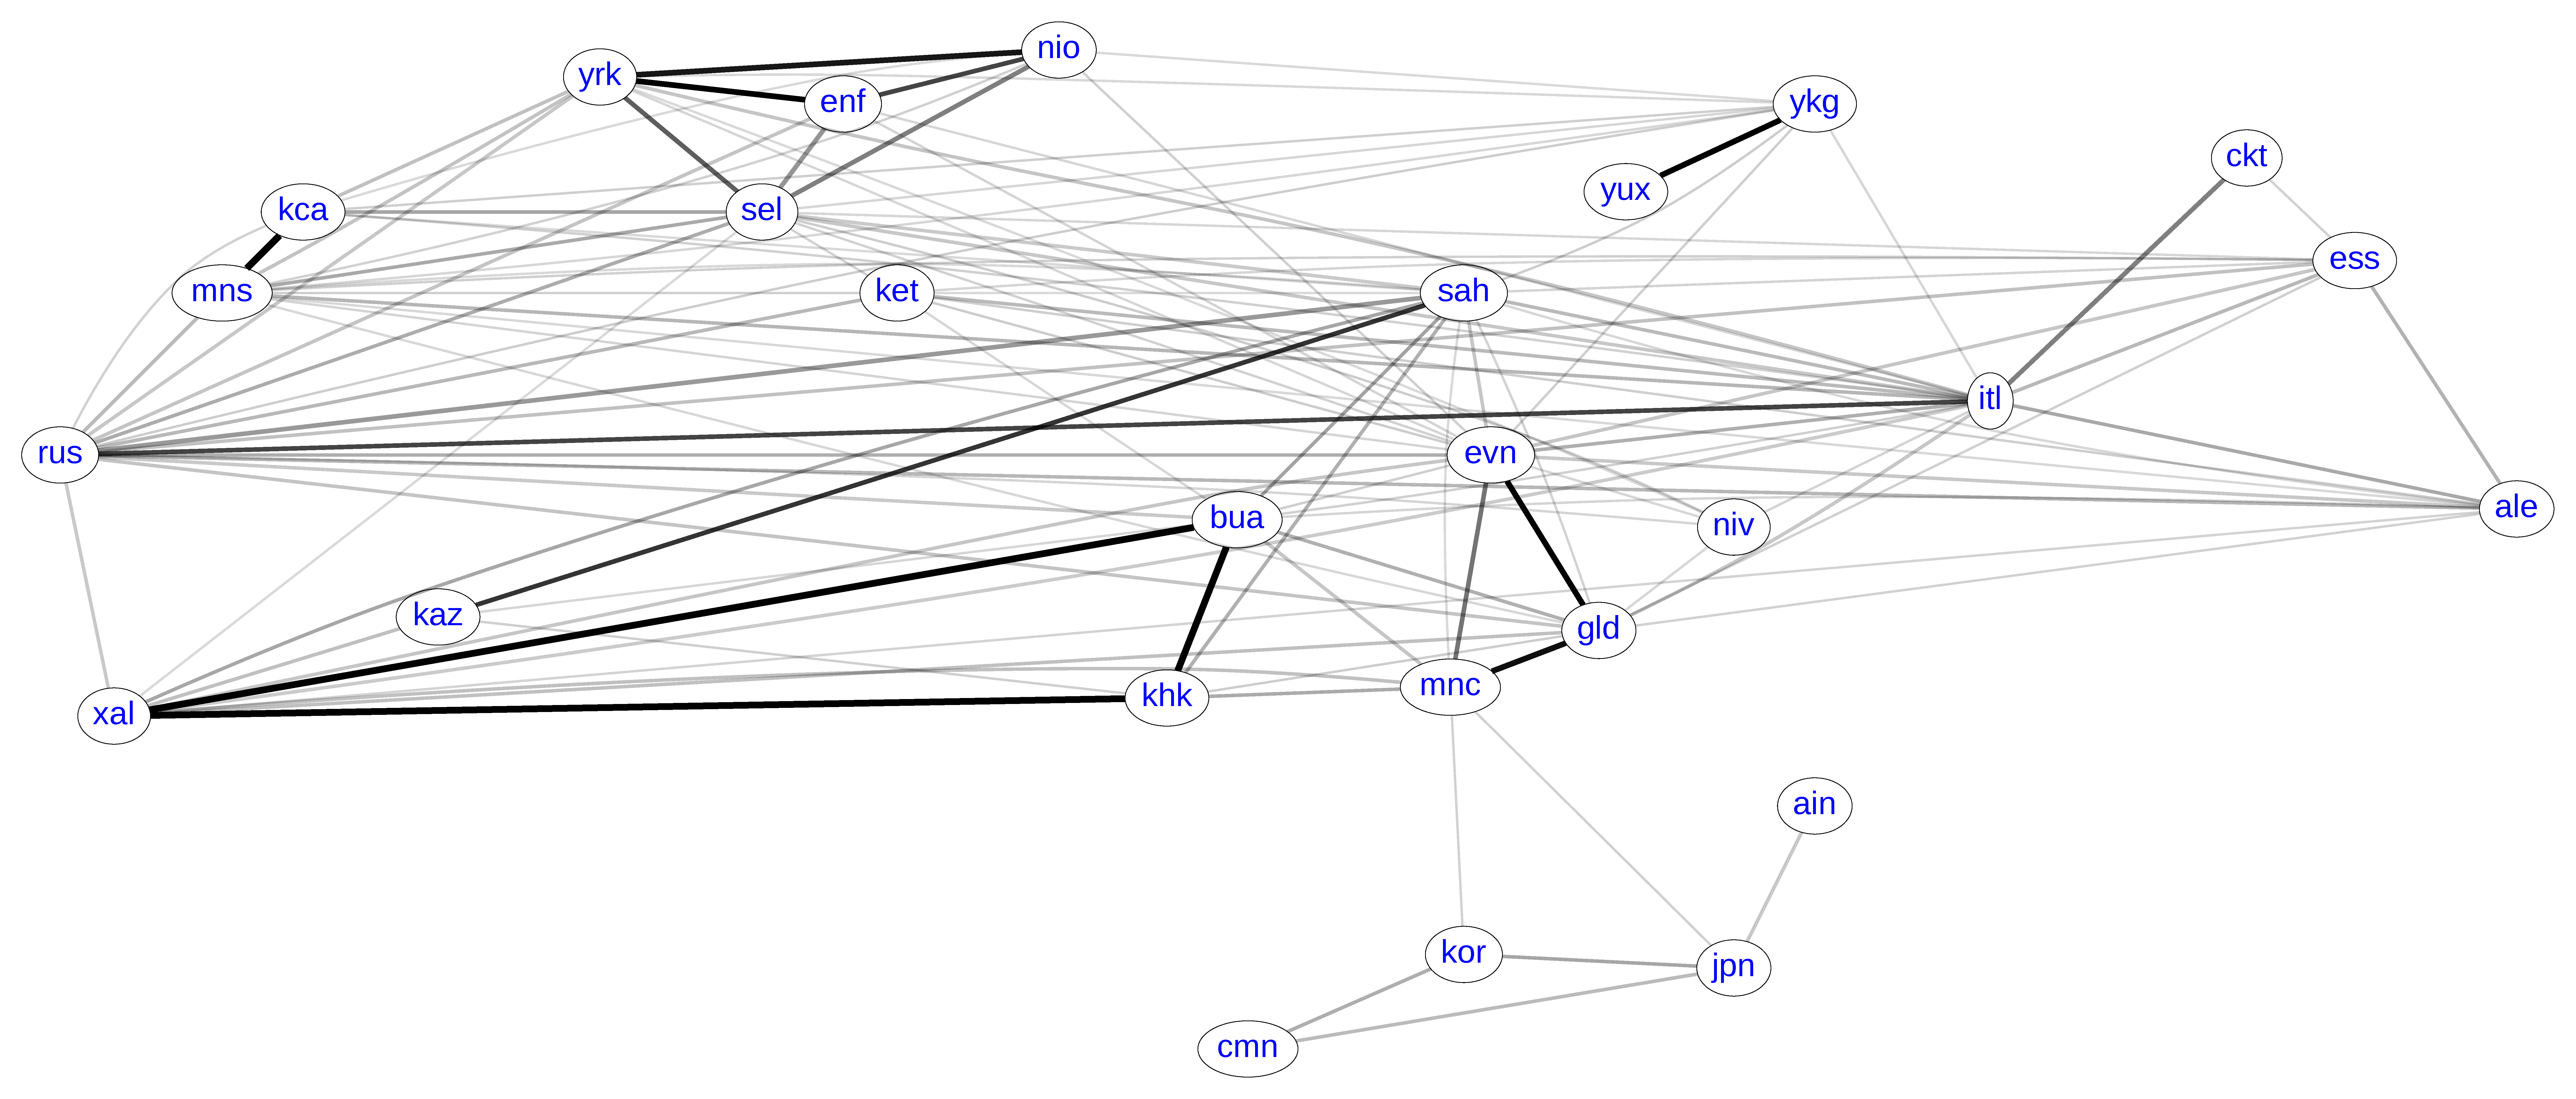
\includegraphics[width=\textwidth]{figures/cognacy-strength-siberia.pdf}
 \caption{Visualization of inferred cognate overlap in the Siberian data}
 \label{siberia-cognacy}
\end{sidewaysfigure}

\figref{siberia-goldstandard-phylo} visualizes the gold standard network arising from the previous discussion. The star shape of arrows from \ili{Russian} into almost all the languages of Siberia show that unlike in the previous two case studies, we now only have one major cause of lexical overlap between the many small families and isolates. The challenge in this case study is the correct detection of the many isolates. For reasons which will become clear in the next chapter, the directionality of influence between an isolate and a member of a different family is difficult to detect for causal inference. The directionality of contacts between isolates has always been a problem for historical linguists, and we cannot expect the less refined automated methods to solve it.

\begin{sidewaysfigure}
 
\includegraphics[width=\textwidth]{figures/goldstandard-phylo-siberia.pdf}
 \caption{Gold standard for phylogenetic flow on Siberian data}
 \label{siberia-goldstandard-phylo}
\end{sidewaysfigure}

\subsection{Case study 4: a visit to the Caucasus}
The Caucasus is by far the linguistically most complex region covered by the NorthEuraLex database. In addition to three indigenous language families, many \ili{Turkic languages}, several branches of Indo-European\il{Indo-European languages} (Iranian\il{Iranian languages}, \ili {Armenian}, and Slavic\il{Slavic languages}), and even a Mongolic language (\ili{Kalmyk}) exist in the region. The Caucasus has been famous for its high density of widely divergent languages since antiquity, receiving the very fitting epithet \textit{\v{g}abal al-alsun} `mountain of tongues' by the Arab geographer al-Mas\textquoteleft udi in the 10th century.

Starting out with the indigenous families, the \textit{Abkhazo-Adyghean} or \textit{Northwest Caucasian} languages\il{Northwest Caucasian languages} (\textit{abk}, \textit{ady}) are a small group of four living languages, which fall into the two primary branches Abkhaz-Abaza\il{Abkhaz-Abaza languages}, consisting of \ili{Abkhaz} (\textit{abk}) and closely related \ili{Abaza}, and the Circassian\il{Circassian languages} dialect continuum, with the literary languages \ili{Adyghe} (\textit{ady}) in the west, and \ili{Kabardian} in the east. Both branches are only represented by a single language in the current version of NorthEuraLex, such that Abkhaz-Abaza will be synonymous with \textit{abk}, and Circassian with \textit{ady}. The Northwest Caucasian languages are typological outliers in Europe, with their predominantly ergative case alignment, phoneme inventories which are very rich in consonants but with minimal numbers of vowels, and, perhaps most interestingly, a very complex verbal morphology where 
verbs agree with up to three arguments, instead of just the subject, as is the case in typical European languages. According to \cite{hewitt2004}, both languages in our sample have borrowed some words from \ili{Turkic languages}. The dominant influence, however, occurred after the \ili{Russian} conquest of the Caucasus (\textit{rus} \arrowLA \textit{abk, ady}). In addition, Abkhaz has come under significant pressure by \ili{Georgian} (\textit{kat} \arrowLA \textit{abk}) as the state language of the Georgian SSR. This pressure has subsided since independent Georgia lost control of Abkhazia after a civil war in 1992, which is now a de-facto independent state without international recognition.

The \textit{Nakho-Daghestanian}\il{Nakho-Daghestanian languages} or \textit{Northeast Caucasian}\il{Northeast Caucasian languages} languages (\textit{che}, \textit{ava}, \textit{lez}, \textit{dar}, \textit{lak}, \textit{ddo}) are spoken mainly in the Russian republics of Daghestan, Chechnya, and Ingushetia. The family is well-known for featuring the world's most extensive case systems, and the largest noun class systems after the \ili{Bantu languages}. NorthEuraLex contains a sample of six Northeast Caucasian languages, falling short of the goal of having one representative on each branch, but containing all the literary languages for which large dictionaries are readily available. The about 40 languages of the family can be grouped into seven uncontested branches, but the structure of the larger subunits is still subject to debate, much as in the case of Uralic. Traditionally, the family was split into a Nakh\il{Nakh languages} branch containing the closely related literary languages \ili{Chechen} (\textit{che}) 
and \ili{Ingush}, and a Daghestanian\il{Daghestanian languages} branch comprising all the other branches. Among the languages of Daghestan, a general consensus seems to be that the \ili{Avar-Andic languages}, to which the lingua franca \ili{Avar} (\textit{ava}) belongs, are more closely related to the \ili{Tsezic languages}, which are represented in NorthEuraLex by \ili{Tsez} (\textit{ddo}), than to the other branches of Nakho-Daghestanian. The other Daghestanian branches are the \ili{Dargin languages} represented by Literary \ili{Dargwa} (\textit{dar}), the \ili{Lezgic languages} represented by \ili{Lezgian} (\textit{lez}), and the isolates \ili{Lak} (\textit{lak}) and \ili{Khinalugh}, the latter of which is not part of NorthEuraLex. While Tsez and many other small Daghestanian languages are endangered, the five large literary languages in our sample can be considered sociolinguistically stable, even though bilingualism with \ili{Russian} is by now almost universal \citep{hewitt2004}. During their history, 
all Northeast Caucasian languages have borrowed substantial amounts of lexical material from \ili{Persian}, Oghuz Turkic\il{Oghuz Turkic languages}, and \ili{Russian}, the languages of neighboring empires vying for control of the Caucasus (\textit{rus}, \textit{pes}, \textit{azj} \arrowLA \textit{che}, \textit{ava}, \textit{lez}, \textit{dar}, \textit{lak}, \textit{ddo}). Influence from smaller \ili{Turkic languages} such as \ili{Kumyk} and \ili{Nogai} has also existed for centuries. Due to the close similarity of these languages with \ili{Azeri} in their basic vocabulary, most of these influences can be subsumed under the incoming lexical flow from Azeri, although some signal will be lost due to the absence of these Turkic languages of the Caucasus in our sample. Finally, Avar has influenced the other languages of Daghestan due to its role as a lingua franca of the region (\textit{ava} \arrowOA \textit{lez}, \textit{dar}, \textit{lak}, \textit{ddo}).

The third language family native to the Caucasus, \textit{Kartvelian}\il{Kartvelian languages} or South Caucasian\il{South Caucasian languages}, consists of the \ili{Georgian} language (\textit{kat}), the only indigenous Caucasian language with an ancient literary tradition, three closely related minority languages which are often treated as variants of Georgian, and more distantly related \ili{Svan}, all of which are not yet represented in NorthEuraLex. Like most languages in the region, Georgian was influenced intensively by \ili{Persian} (\textit{pes} \arrowLA \textit{kat}) and \ili{Turkic languages} (\textit{azj} \arrowLA \textit{kat}). Russian influence on basic vocabulary is rather limited in comparison, because Georgian was influenced much more from its southern neighbors when its statehood and cultural identity was formed in the Middle Ages. \cite{khalilov1993} systematically describes the language contacts between Georgian and neighboring \ili{Northeast Caucasian languages}. The main conclusion 
is that the borrowings from \ili{Daghestanian languages} into eastern dialects of Georgian do not appear in the Georgian literary language, and should therefore not be visible in our dataset. In the reverse direction, intensive borrowing took place in the nominal domain, where also many Iranian\il{Iranian languages} loans were transmitted into Daghestan via Georgian. The only two Daghestanian languages in the sample whose lexicon was significantly influenced by Georgian are \ili{Avar} (\textit{kat} \arrowLA \textit{ava}) and \ili{Tsez} (\textit{kat} \arrowLA \textit{ddo}), the immediate eastern neighbors of Georgian. Contacts with \ili{Nakh languages} such as \ili{Chechen} did exist, but did not leave substantial traces in the basic vocabulary of either Georgian or Chechen.

The \textit{Iranian}\il{Iranian languages} branch of Indo-European (\textit{kur}, \textit{pes}, \textit{oss}, \textit{pbu}) has been one of the decisive factors which shaped the linguistic landscape of the Caucasus. The Iranian languages are classified into the two subgroups Western Iranian\il{Western Iranian languages} and Eastern Iranian\il{Eastern Iranian languages}, each of which can be separated into a northern and a southern branch. NorthEuraLex contains the dominant language of each of the four groups.

\ili{Ossetian} (\textit{oss}), one of two extant Northeast Iranian languages (the other being \ili{Yaghnobi} in Tajikistan), is taken to be a direct descendant of the \ili{Scytho-Sarmatian languages} spoken by Iranian peoples all over the Central Asian steppes since the 8th century BC. Modern Ossetian is split into two varieties, the larger of which, Iron, is spoken by about 570,000 speakers in both North and South Ossetia, and is the variant represented in NorthEuraLex. According to \cite{thordarson2009}, evidence from placenames in the Northwest Caucasus suggests that the Ossetes once lived further to the west, where Turkic\il{Turkic languages} and \ili{Circassian languages} are spoken today, and that a Nakh language related to \ili{Ingush} was spoken in North Ossetia. These interactions have left their traces in the lexicon, and Iron Ossetic contains layers of loanwords from Circassian (\textit{ady} \arrowLA \textit{oss}), Nakh (\textit{che} \arrowLA \textit{oss}), and Turkic languages (\textit{Turkic} \arrowLA \textit{oss}).

\ili{Pashto} (\textit{pbu}), the only important Southeast Iranian language, is spoken by about 50 million people in Southern Afghanistan and Northern Pakistan. Modern Pashto is not of immediate relevance to the Caucasus, but an important second datapoint in addition to Ossetian for reconstructing the cognate sets present in Eastern Iranian, which can be expected to lead to a clearer picture. The two largest lexical influences on Pashto are \ili{Persian} and \ili{Hindi}-\ili{Urdu} (\textit{pes}, \textit{hin} \arrowOA \textit{pbu}), the languages of neighboring states with a lot of cultural influence on the mountains inhabited by Pashtun tribes. Some additional religious and scientific terminology was borrowed directly from \ili{Arabic} as well (\textit{arb} \arrowLA \textit{pbu}).

Modern \ili{Persian} (\textit{pes}), the only major Southwestern Iranian language, is spoken under different names in Iran (Farsi), Northern Afghanistan (Dari), and Tajikistan (Tajik). As the state language of the Persian empire as well as modern Iran, and the predominant language of literature and science in the region, Persian has been a major source of lexical material for all neighboring languages, including \ili{Turkish} and \ili{Hindi}. In these contacts, Persian also served as a transmitter language for much religious and scientific vocabulary which the Persians borrowed from the Arabs together with Islam (\textit{arb} \arrowLA \textit{pes}). Loans from Turkic\il{Turkic languages} and \ili{Mongolic languages} into Persian do exist, but they are mostly confined to the military and the administration.

By far the most important Northwestern Iranian language is \ili{Kurdish}, with an estimated 30 million speakers. Of the different variants of Kurdish, NorthEuraLex samples the \ili{Kurmanji} language (\textit{kmr}) by a dialect spoken in Turkey near the Syrian border, i.e.\ in the center of the Kurdish-speaking lands. During its history, all variants of Kurdish have borrowed substantially from their \ili{Arabic}-speaking southern neighbors (\textit{arb} \arrowLA \textit{kmr}), and to a much lesser degree from the Armenians\il{Armenian} to the north. Also, as any state language on a minority language, Turkish has left lexical traces in the NorthEuraLex variant Kurmanji (\textit{tur \arrowLA kmr}), whereas an Iranian variant would have displayed a strong recent influence from Persian.

\ili{Armenian} (\textit{hye}), the oldest Indo-European language of the Caucasus, forms a separate branch of the family, with possible deep affinities to \ili{Greek}. In addition to a layer of very early loans from Kartvelian\il{Kartvelian languages} (\textit{kat} \arrowLA \textit{hye}) and some borrowings from \ili{Northeast Caucasian languages}, Armenian has been under pervasive influence from various \ili{Iranian languages} throughout its history, to the point that it was long itself considered an Iranian language. \cite{bailey1987} discusses the different layers of Iranian loanwords which have been the subject of more than a century of research, and are so rich that their analysis contributed to a better understanding of the development of Middle Iranian. Since some of the loans go back as far as the Old Iranian period, it makes sense to include \textit{Iranian} \arrowOA \textit{hye} in the gold standard in order to model the ancient connections. As later cultural vocabulary overwhelmingly came from 
variants of \ili{Persian}, I additionally include a link \textit{pes} \arrowOA \textit{hye}.

Turkic presence in the Caucasus goes back to the arrival of Oghur tribes in the 7th century, who formed the Bulgar and Khazar khanates in the Pontic and Caspic steppes. Too little is known about these languages to decide whether Turkic loans in the North Caucasus can be traced back to this time, or whether they occured during the time of the Pecheneg khanates, who occupied the same area in the 10th and 11th centuries. The influence of their \ili{Pecheneg} language, which belongs to the Oghuz\il{Oghuz Turkic languages} branch of Turkic, is approximated in the gold standard by \ili{Azeri} (\textit{azj}). The next Turkic-speaking steppe state, the Cuman-Kipchak confederation of the 12th century, brought the Kipchak languages\il{Kipchak Turkic languages} spoken by today's Turkic inhabitants of the North Caucasus, such as \ili{Karachay-Balkar} in the Northwest Caucasus, the \ili{Nogai} language in the center, and \ili{Kumyk} in Northern Daghestan. These languages especially influenced the \ili{Circassian 
languages}, \ili{Chechen}, and the Northern Daghestanian languages \ili{Dargwa} and \ili{Avar} (\textit{Kipchak} \arrowLA \textit{ady, che, dar, ava}). All of these contacts will be represented by means of the only Kipchak language, \ili{Kazakh}, in the language sample for this case study. As an additional datapoint, I also add \ili{Uzbek} (\textit{uzn}) to the dataset, which does not appear to have any relevant contacts into the Caucasus beyond the Common Turkic layer represented by the other three languages. On the south side of the Caucasus, \ili{Ottoman Turkish} borrowed extensively from Arabic (\textit{arb} \arrowLA \textit{tur}), the language of the southern half of the Ottoman Empire, and in turn influenced the \ili{Arabic} dialects in Syria and Iraq. Like most languages of the region, Turkish, Azeri, and Uzbek have many loans from \ili{Persian} (\textit{pes} \arrowLA \textit{tur, azj, uzn}).

Eastern influences on \ili{Russian} (\textit{rus}) and the lexical sources for the Mongolic language Kalmyk (\textit{xal}) were already discussed in the previous section. The \textit{Semitic} languages\il{Semitic languages} represented in NorthEuraLex, \ili{Arabic} (\textit{arb}) and \ili{Hebrew} (\textit{heb}), were not strongly influenced by any languages from the north. Still, Arabic needs to be included as an important source of religious and scientific vocabulary for the entire Islamic world. Hebrew, the most important Northwest Semitic language which shares hundreds of cognates in basic vocabulary with Arabic, did not interact much with any languages of the Caucasus area, but still seemed worthwhile to include as a test case for the absence of lexical flow.

The cognate overlaps visualized in \figref{caucasus-cognacy} show that the lexical flow inference problem on this set is again different in structure from the other three example scenarios. This time, there are multiple poles causing lexical overlaps across much of the region, as Arabic, Iranian, Russian, and Turkic material are all very widespread. A large part of the lexical flow inference task consists in answering the question whether e.g.\ some of the overlaps with Arabic can be explained away by Persian or Turkic as intermediates.

\begin{figure}
 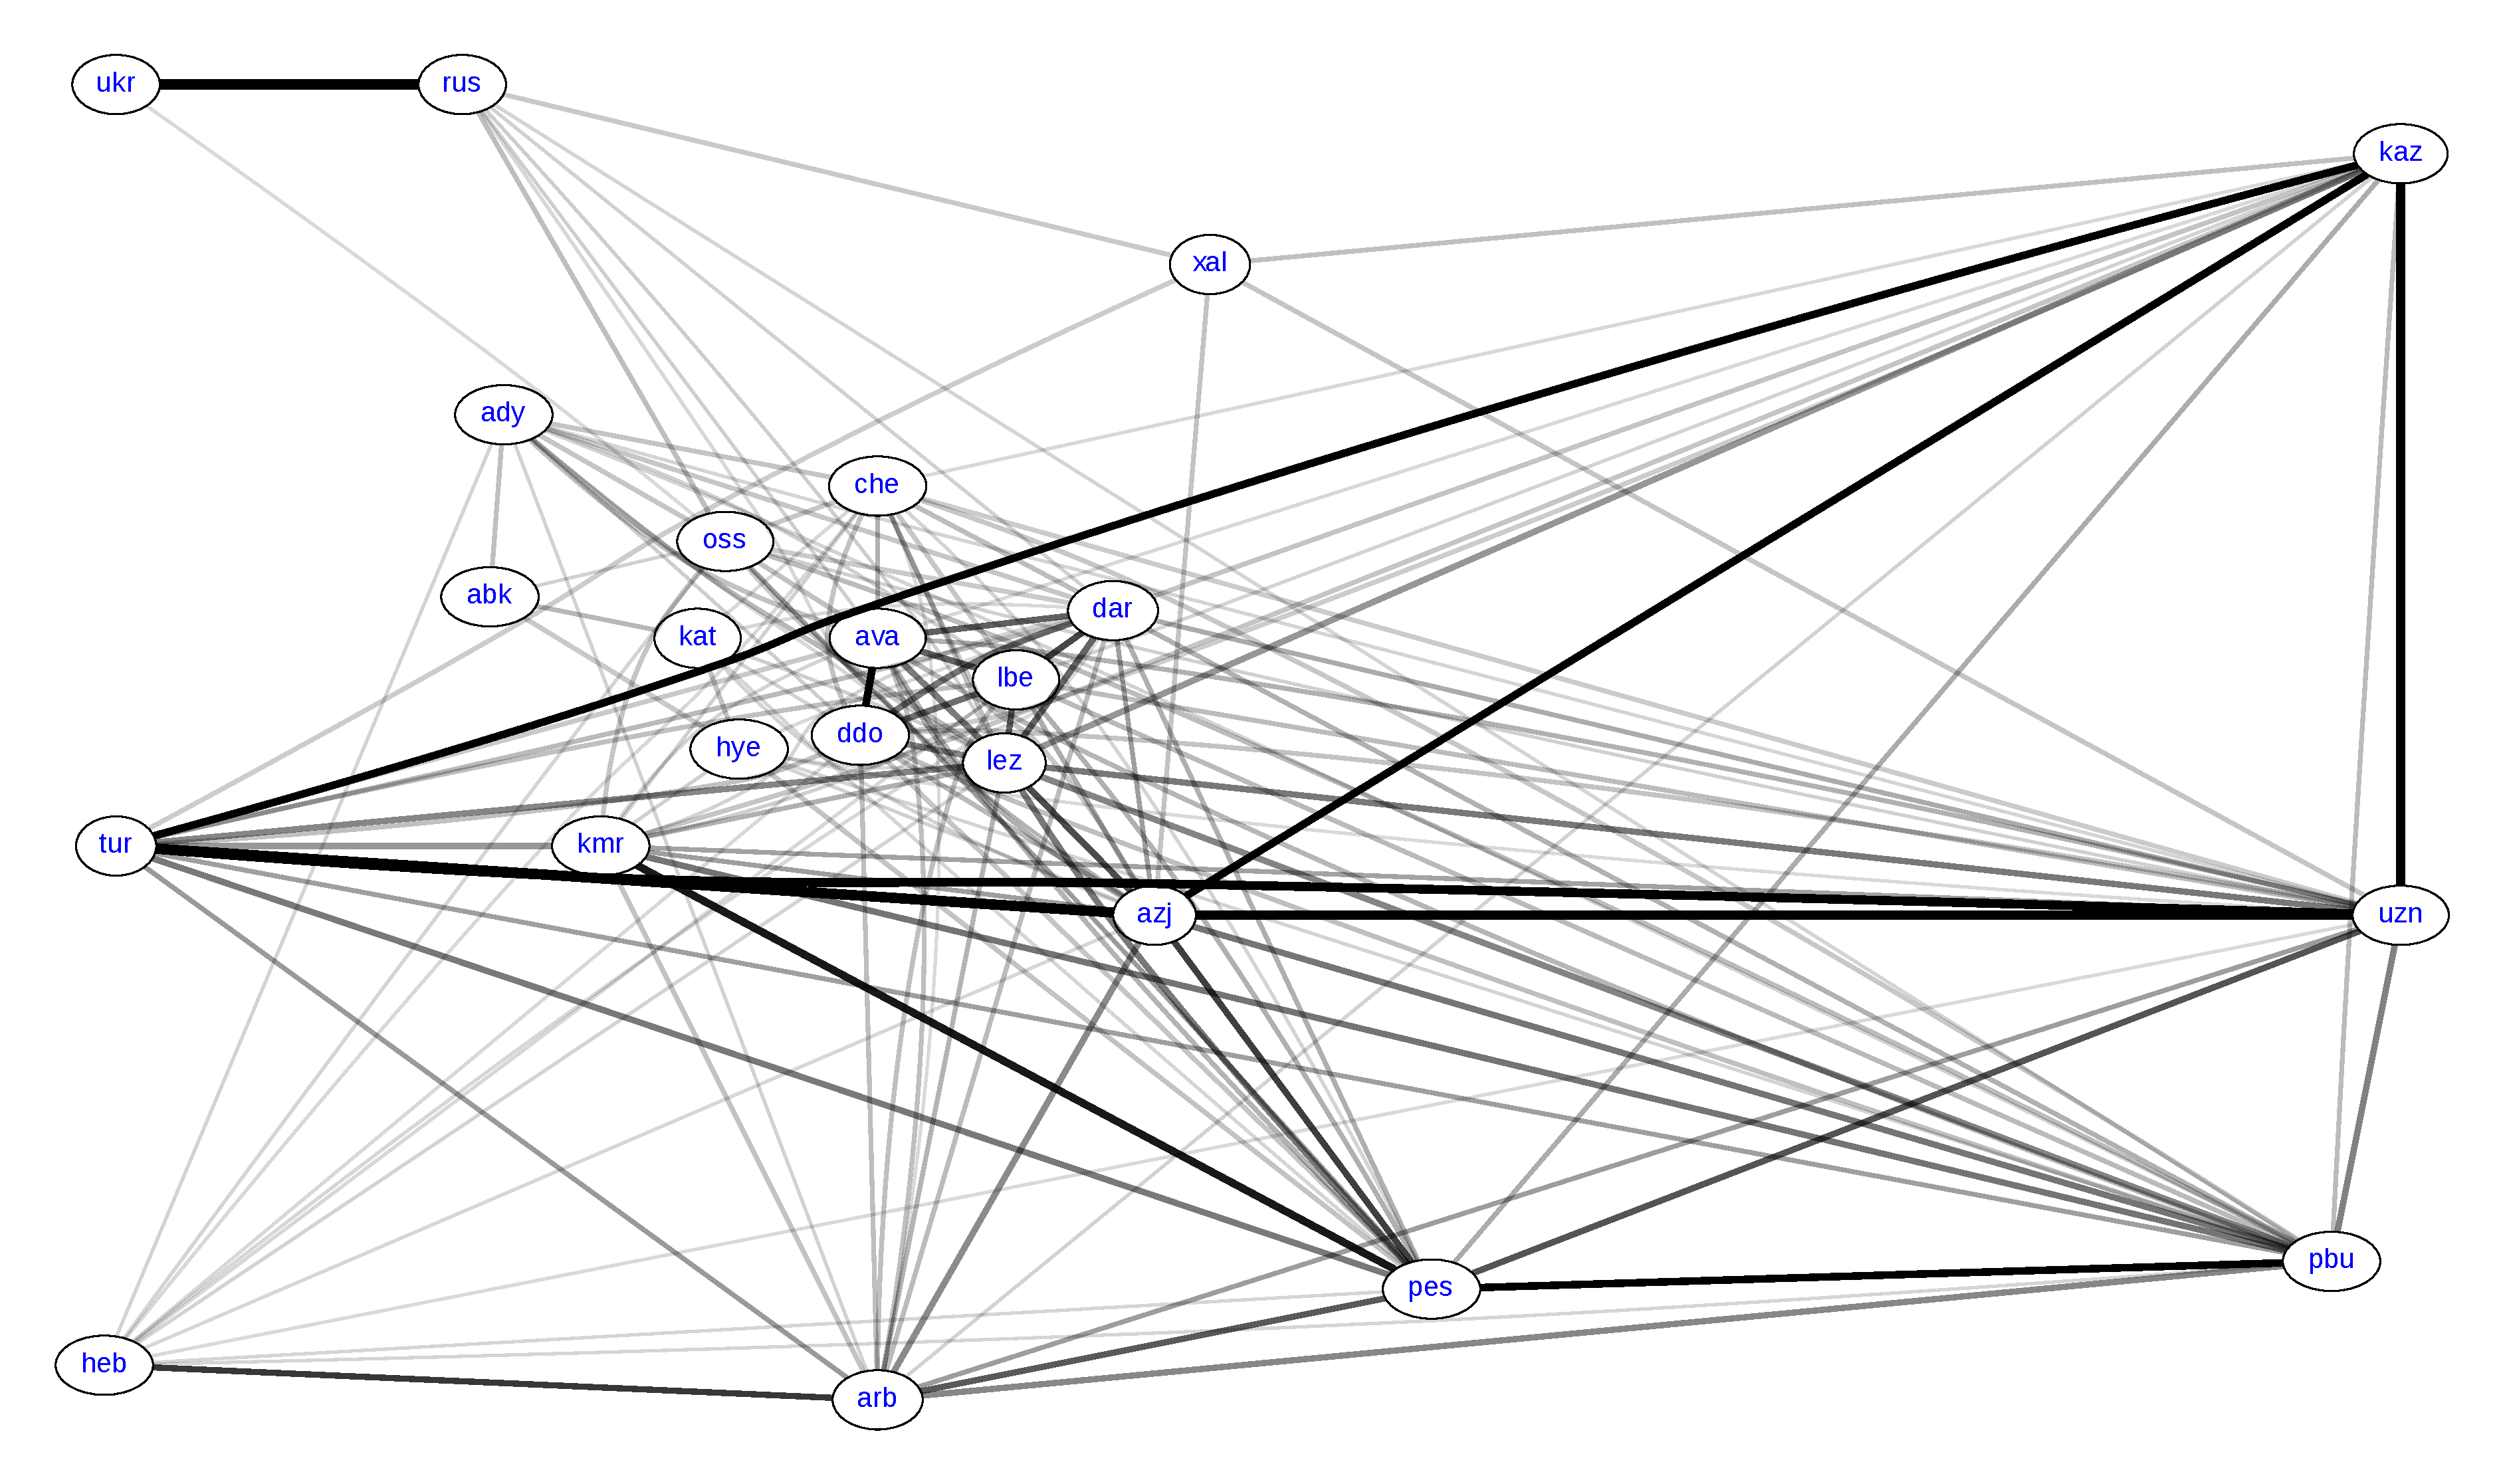
\includegraphics[width=\textwidth]{figures/cognacy-strength-caucasus.pdf}
 \caption{Visualization of inferred cognate overlap in the Caucasian data}
 \label{caucasus-cognacy}
\end{figure}

\figref{caucasus-goldstandard-phylo} shows the gold standard for phylogenetic inference. It is easy to glimpse that this scenario is by far the most challenging to get right, due to the very complex interactions among the native languages of the Caucasus, which are additionally influenced by the four major external sources of lexical material mentioned above. 

\begin{figure}
  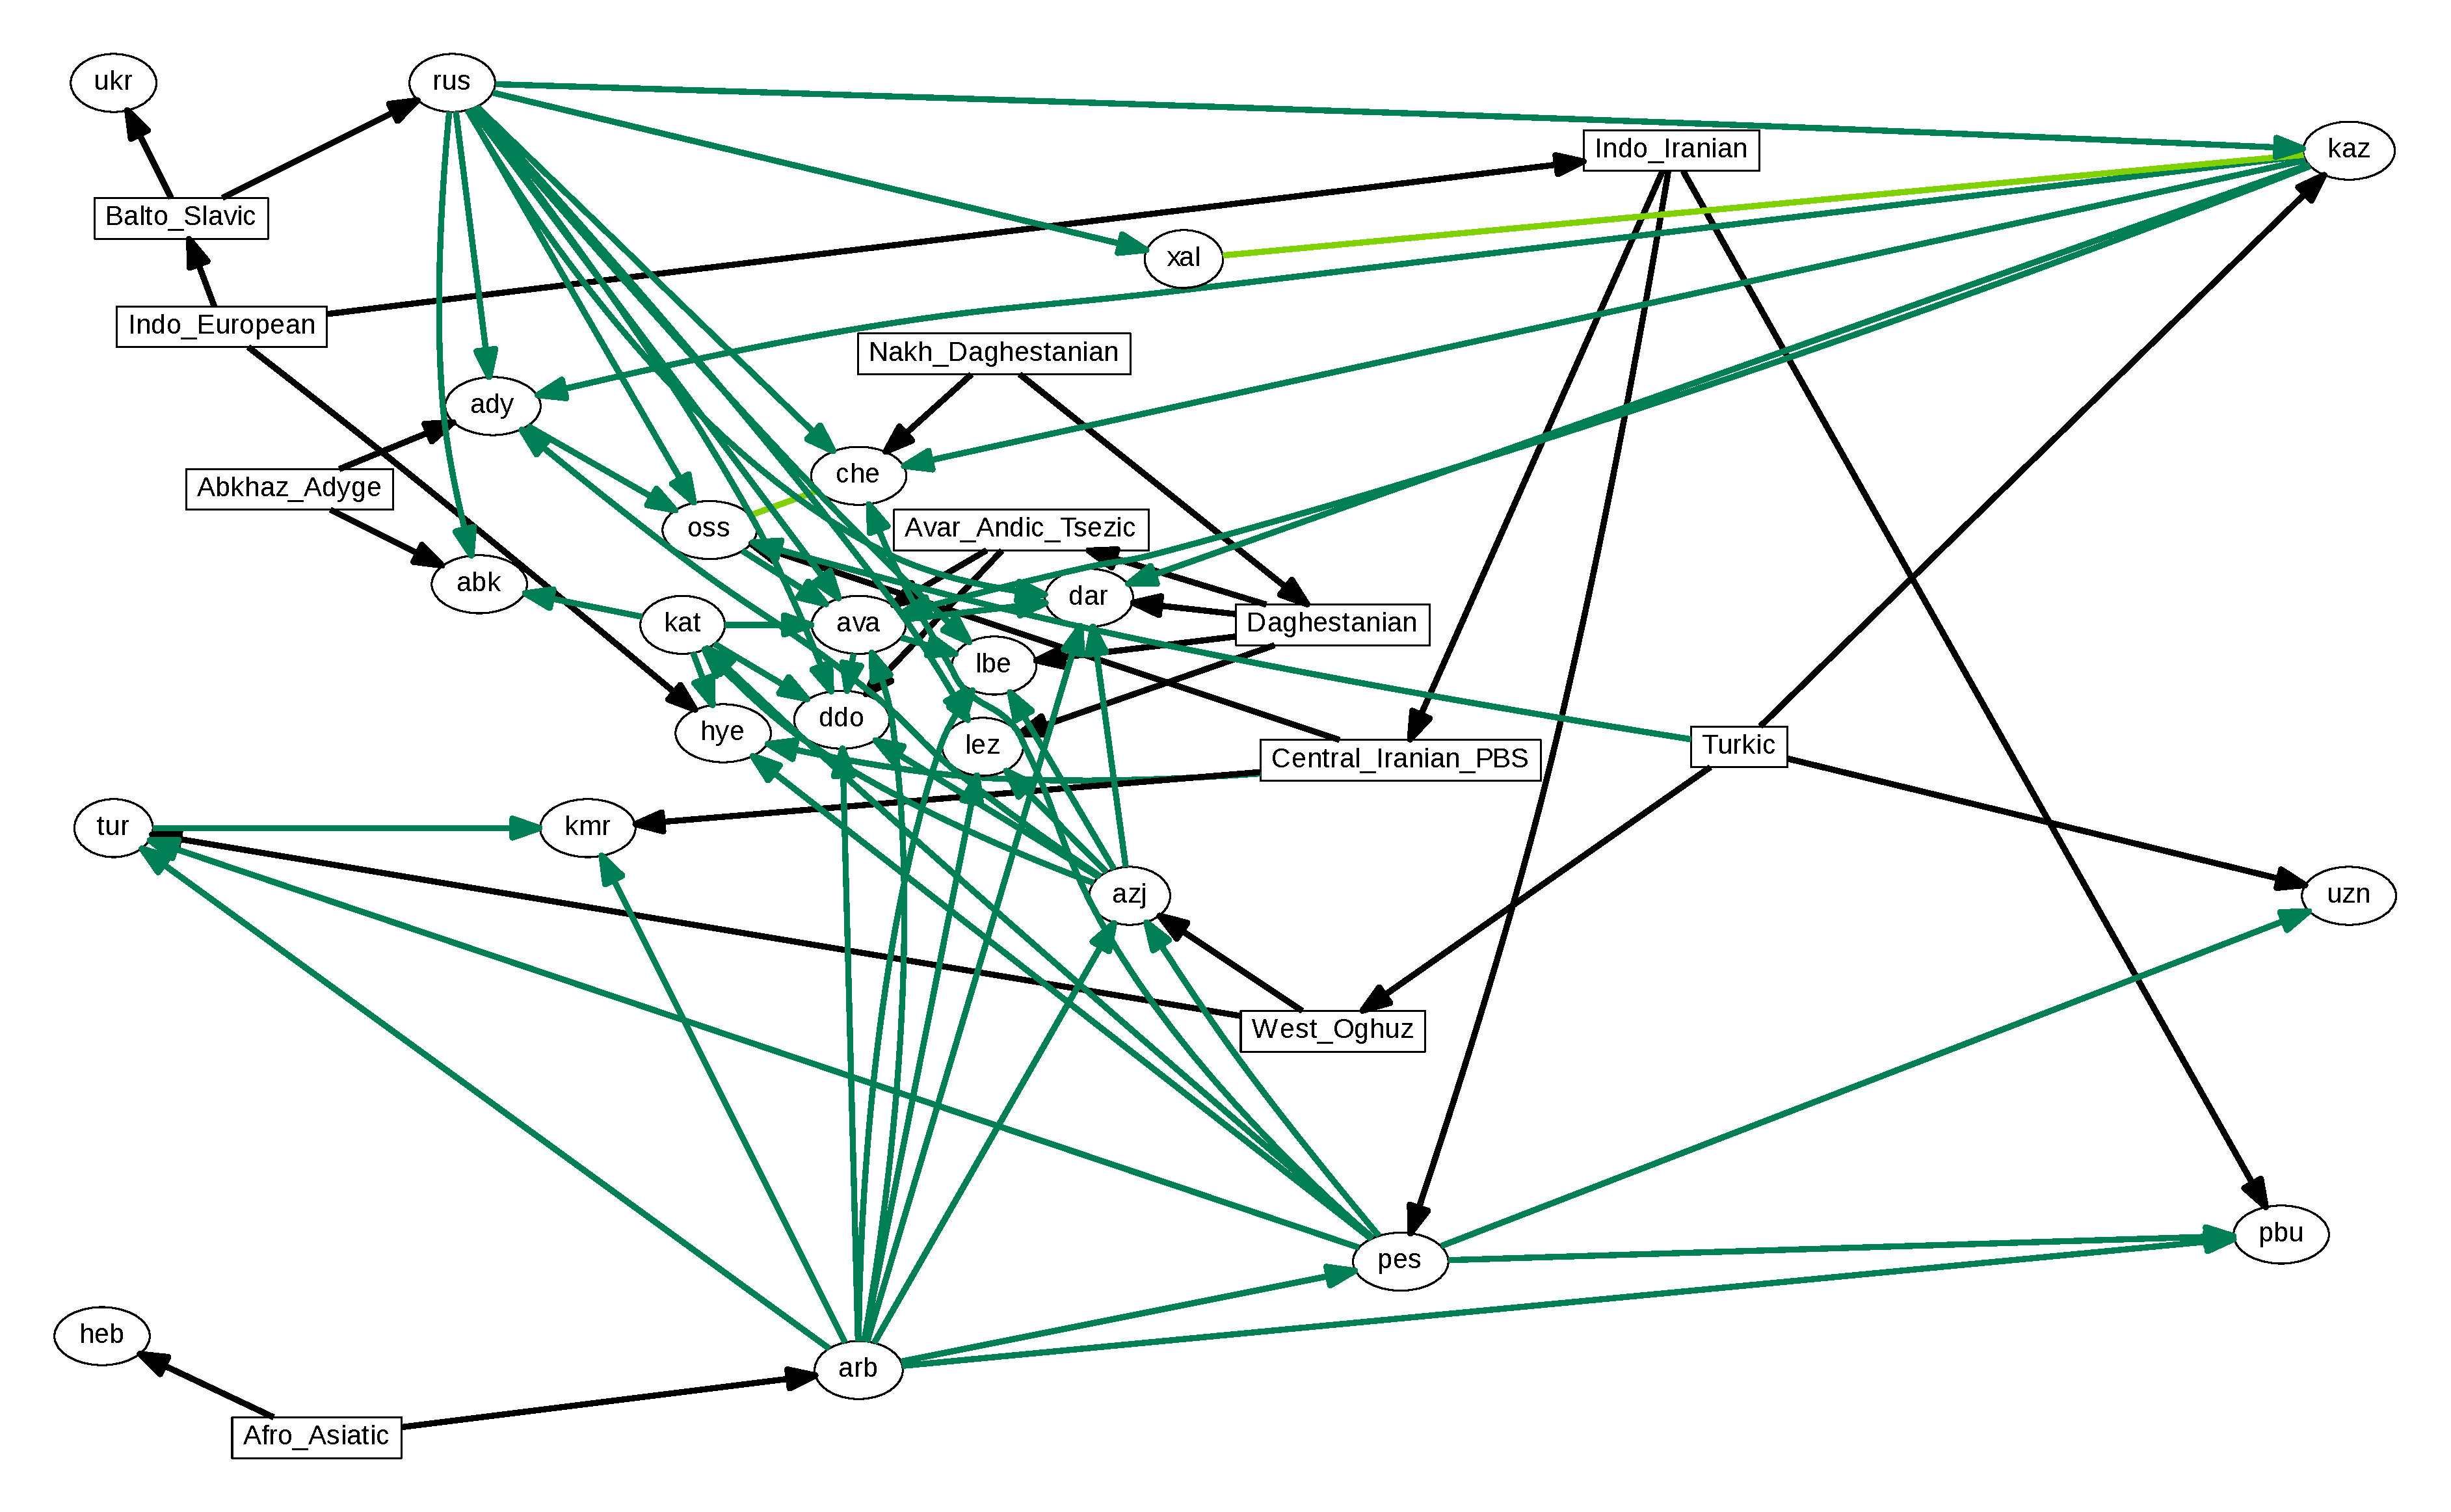
\includegraphics[width=\textwidth]{figures/goldstandard-phylo-caucasus.pdf}
  \caption{Gold standard for phylogenetic flow on Caucasian data} 
  \label{caucasus-goldstandard-phylo} 
\end{figure} 

After presenting the four test scenarios derived from true linguistic histories, we now turn to the way in which any number of additional test scenarios can be synthesized in order to gain a better picture of the comparative performance of different approaches to lexical flow inference.

\chapter{Simulating cognate histories}\label{sec:5}
After some general remarks on the place of simulation studies in computational historical linguistics as well as the in-silico approach to evaluation, this chapter presents the simulation model which I am using in parallel to the NorthEuraLex data to evaluate lexical flow inference methods.

Unlike more detailed existing simulation models like \cite{hochmuth_ea_2008}, which have components for explicitly generating and modifying phonetic strings and modeling the geographical spread of languages, my model limits itself to modeling contact in the form of transmitting discrete units, i.e.\ it models loanwords on the level of cognacy, without generating actual phonetic forms. This creates data different from what historical linguistics would apply to decide whether lexemes were inherited or borrowed, but the shape of the data is exactly what will be needed to evaluate lexical flow inference algorithms. 

\section{Simulation and in-silico evaluation}

\subsection{Advantages and shortcomings of simulation}
A simulation model is an algorithm which models the behavior of some real-world system, and uses randomness to generate output which is similar to the output of the real system. For instance, an adequate model of an economy should generate time series of measures such as interest rates, inflation, and unemployment which behave just as erratically as their real-world equivalents. An adequate model of tree growth should generate trunk shapes and branch structures which look just like the ones we can observe on real trees.

A very popular application of simulation models is as a way of testing assumptions about how the actual data can be explained. If our model generates data which are indistinguishable from our real data according to some relevant measure, we can take this as evidence that we have correctly understood and formalized an interesting aspect of the problem.

Within linguistics, this paradigm has previously mainly been applied to language competition. \cite{schulze_ea_2008} give an overview of different attempts to let a distribution of language sizes (by number of speakers) emanate from minimalistic models, with the goal of mirroring the observable distribution as closely as possible. Many of the more successful models are agent-based, modeling individual speakers which can choose to take over the language of neighboring speakers based on a prestige value, or just the dominant language in the neighborhood.

Combining previous models for explaining the distibution of language sizes, \cite{oliveira_ea_2008} arrive at a model which captures the observable distribution of language family sizes. While the final model given in the appendix of the paper is rather simple, the authors report that in additional experiments, adding more complexity to the models (e.g.\ by including the effects of war and similar historical contingencies) did not have any influence on the overall good fit with observed family sizes. I will take this as an indication that attempting to include such effects into my model is just as unlikely to lead to different behavior, allowing me to keep my own simulation simple as well.

Establishing knowledge about real-world systems on the basis of simple simulations is frequently criticized as too reductionistic, and spectacularly wrong predictions resulting from simulation models may have contributed to wide-spread scepticism towards modern economic theories. The practical and far less controversial advantage of simulation models is that they allow us to generate arbitrary amounts of data to test algorithms on. This in-silico evaluation allows us to compensate for insufficient amounts of actual test data, or as additional cross-validation of models developed on (and optimized for subsets of) actual data.

This is the paradigm in which \cite{embleton1986} already worked. Her simulation model represents an early attempt to adequately model the influence of borrowing between neighboring languages on cognate-based phylogenetic inference. The model is similar in spirit to the one I am presenting in this chapter, in that it operates on the level of individual cognate replacement events. Unlike my model, it assumes that the process of language split can be modeled by recursive subdivision of a two-dimensional area, precluding the possibility of geographical spread. Also, borrowing events are modeled as independent, i.e. for every new borrowing event sampled according to a global borrowing rate, a language picks one of the neighboring languages as the donor language at random, whereas the model I present in this chapter samples an additional level of contact channels in order to mirror the strong tendency for loans to occur in `packages' triggered by historical events. 

\cite{murawaki2015} presents another approach which explicitly simulates the transmission of lexical items by borrowing among neighboring language varieties, but does not have a phylogenetic component. The structures produced are thus very similar to my concept of contact flow networks. Based on the cognacy overlaps resulting from simulation on different network typologies, Murawaki then performs phylogenetic analysis, with the somewhat surprising result that the phylogenetic signal tends to look tree-like on tree-like spatial structures, even if inheritance is not modeled. This could indicate that the usually very good fit of tree models does not necessarily have to result from tree-like evolution, but that wave-like change can just as easily lead to tree-like signals in certain geographical configurations, which has interesting implications for the debate between family tree and wave models of language change.

Unlike the other models, the rather complex simulation model by \cite{hochmuth_ea_2008} generates phonetic data, to which the authors then apply modern standard tools for phylogenetic tree and network inference. While they find the amount of simulated lateral contact to have little impact on the performance of tree inference algorithms, the behavior of phylogenetic network algorithms is described as very erratic.

The main difficulty in using simulation models is that they are necessarily based on a set of assumptions about the nature of the data, which might not be true in reality. What if the way in which we generate data fails to capture an important case that occurs in real data, and is then not covered by the algorithm which we developed and tested on simulated data? To keep this problem under control, it is always best to evaluate a system both against simulated and real data. In the realm of causal inference, there has been a very strong tendency to develop the theory and algorithms either on very well-studied toy examples, or on massive amounts of simulated data. This makes it difficult to assess the performance of these methods on large real-world datasets, a problem that we are going to be faced with again when evaluating their potential for lexical flow inference.

\subsection{Principles of in-silico evaluation}
When assessing the performance of a heuristic algorithm (i.e.\ one without provable properties), the classical framework is to collect a set of gold-standard data, and to let the algorithm run on the data, comparing the output to the gold-standard using a useful definition of true and false positives and negatives, and then quantifying the performance in terms of precision and recall. Since gold-standard data are often difficult to acquire in large quantities (the last chapter provides a very good example of the efforts that may be required), the conclusions made from evaluating an algorithm on real data often rest on unstable grounds.

In the absence of a large enough amount of gold-standard data, one can use simulated data to get an impression of how the algorithm would perform on other data of the same shape. To get informative results, quite a bit of effort needs to be invested into developing a simulation model which is adequate for the purpose. The main requirements are that the model should not be overly complex in order to decrease the risk of overfitting the algorithm to certain (possibly hidden) properties of the gold-standard data. In a simulation model, it is always tempting to capture all aspects of the real data, but such an approach will often require many decisions to be made with inadequate backing in data or theory.

For instance, the actual linguistic history of a region is shaped by many historical events such as invasions, political ideas, technical innovations, and the shape of trade networks. A simulation model could try to emulate all of these phenomena in order to arrive at realistic simulated histories, and use these events to generate linguistic data. The problem is of course that such a model would require a very explicit (and formalized or at least quantitative) theory of political events, predictions about the conditions under which they will occur, and many other components which would quickly explode into separate research projects if we want to justify all of the myriad decisions which would be involved in designing such a model. Keeping the model complexity low, and the number of design decisions at a minimum, helps to avoid introducing too many unwarranted assumptions.

To configure the parameters even of a small model, it is good scientific practice to use structural features or at least statistics estimated from real data to increase (and quantify) the amount of realism. For instance, we might want to put data on historically observed unemployment rates into an economic model, to estimate how strong we expect oscillations in this measure to be in reality. For a simulation of language history, we will need to estimate (and inform the model) how often languages tend to split, and how intensively they can borrow from neighboring languages.

\section{Generating phylogenies}
A core component of any simulation model in computational historical linguistics (and also of some of the more advanced statistical methods) is a generative description of possible tree shapes. In statistical methods, these models are used to efficiently sample the space of possible trees in order to find good phylogenies. In in-silico evaluation, some part of the generated tree is removed from the input data for an algorithm which tries to reconstruct the missing information, and can then be evaluated against the truth.

Evolutionary models of species trees in biology as in linguistics are minimally based on two modules: the first one describes how languages or species split, and the second one models the process of languages or species becoming extinct. Moreover, if we explicitly model a genome, at least the possible mutations during inheritance need to be modeled. In all these respects, the simulation model presented here makes very simple assumptions in order to avoid dependence on too many parameters and choices. If even a simple model yields cognate histories which are interesting enough for evaluation, there is no reason to introduce additional complexity.

\subsection{Models of lexical replacement}
On the level of cognate sets, the central evolutionary process to take into account is the gradual replacement of existing words for many basic concepts with new lexical material. Semantic change is a phenomenon which appears to occur even in geographically isolated languages, and should therefore be modeled as a language-internal process. Internal replacement of words is also the main mechanism which makes the descendants of an ancestral language which has split dissimilar over time.

While some results suggest that semantic change happens more quickly for some concepts than for others \citep{pagel_ea_2007}, and that these different rates of lexical replacement have cognitive correlates \citep{vejdemo_hoerberg_2016}, for simplicity we will assume both that semantic change occurs at equal speed to all concepts, and that the rates are constant across languages. Any other design choice would lead to additional parameter settings which are difficult to motivate on the basis of available literature, and at the time depth of 5,000 years we will be simulating, the possible existence of ultraconserved words in real data is not much of an issue.

A constant replacement rate $\rho$ is the only parameter which defines the behavior of lexical replacement. $\rho$ defines the probability for a given word in a given language to be replaced by a word from a new cognate set during the current simulated year. We are therefore not simulating semantic change that would lead to loss of differentiation between concepts, and since we will only consider cognate sets for each concept separately, we also do not model the fact that the new cognate set for a concept might arrive there by extension from a different concept.

In the simulations I am running, the base replacement rate is set to $\rho := 0.00036$. This is the rate we arrive at if we assume a retention rate of $70\%$ after 1,000 years. I am setting the retention a bit lower than the 81\% derived for a 215-concept list by \cite{swadesh1955} to account for the unavoidable presence of lower-stability concepts in a list of 1,000 concepts. Most of the early assumptions about retention rates, especially their constancy across time, has been rejected in many individual cases by subsequent research. In a computational study covering three large language families, \cite{atkinson_ea_2008} substantiate the suspicion that lexical change tends to occur in bursts, rather than gradually. In order to keep the number of parameters low, I still stick to Swadesh's original model while acknowledging that the assumption of a constant replacement rate across languages, concepts, and time is a very rough approximation to a much more complex reality. It is worth noting, however, that this does not mean I am assuming a constant effective replacement rate. As I am going to demonstrate, the combination of a Swadesh-style fixed base rate with a fully developed model of borrowing does yield quite realistic variation in the effective replacement rate. I therefore see no immediate need to further complicate the model by an additional parameter, even though the vast majority of contemporary models tend to treat the replacement rate as a further parameter that itself varies across time and across language varieties.

\subsection{Simulating how languages split and die}
With language-internal lexical replacement in the model, all that is needed for a basic model of linguistic evolution is a model of the process by which a language splits into several descendants, and the disappearance of languages. For a realistic model of splits, we would need an explicit geographical model where every language takes up a certain territory, where a larger territory would make it more likely for the language to develop dialects and then split. Moreover, the process should be modified by the possible presence of stabilizing factors such as states, and the ease at which people can migrate throughout their language community. For a good model of extinction, we would similarly have to model at least the effect of armed conflicts, competition between languages of different prestige and cultures at different technology levels, natural disasters, and assimilation processes within states.

Instead of trying to model all these details (a process which would again involve many decisions that are difficult to justify), we resort to a popular basic model of species evolution in biology. A \isi{branching process} is a Markov process describing the development of a number of nodes each of which generates some number of children with a given probability at each discrete time step. If the possible values for the number of children are $0$, $1$, and $2$, we are modeling a process where branches of the population can die out, stay at the same size, or multiply. These three options are sufficient to generate any binary branching language tree. The simplest parametrization results when we set the probabilities for each number of children to $p(2) := \sigma,\ p(1) := 1 - \sigma$. In this formulation, we can interpret the parameter $\sigma$ as the split rate, expressing how likely it is for a language to disintegrate into two separate languages.

To simulate how languages become extinct, we could simply assume an extinction rate $\delta$, and delete during each simulated time unit each language from the tree with this probability. However, previous research summarized by \cite{holman2005} has shown that the distribution of language family sizes and tree shapes generated by such a branching process differs significantly from the patterns we observe in actual language trees.

To arrive at more realistic datasets, it seems necessary to adapt at least a very simple model of geography in order to simulate at least some of the effects of competition between languages, and the survival of remnants of older language families in isolated geographical positions, such as islands and mountain valleys. My central modeling assumption is that languages never disappear if left alone, but only because speakers of another language migrate and become dominant (e.g.\ \ili{English} in North America), a state conquers a new territory and imposes its language on the newly acquired population (e.g.\ the Roman Empire in Gaul, or later colonial empires), or a population shifts to a more prestigious language for economic reasons (e.g.\ from \ili{Livonian} to \ili{Latvian}, and many other minority languages). The crucial point is that I will assume extinction to happen exclusively due to the spread of another language. Even if exceptions to this rule might exist, I consider this a much more sensible 
default assumption than to assume that some languages just happen to become extinct without being in contact with other languages.

My model subsumes all of these situations by having a language that splits expand into a neighboring territory, which might previously have been occupied by another language, which then becomes extinct during the process. That said, a splitting language will always prefer to spread into an unoccupied territory first, so that the map will tend to become filled with languages before competition and replacement sets in. To create geographical niches in which less frequently splitting families can survive longer (the Caucasus), and hub areas were languages tend to replace each other much more frequently (the Steppes), only a randomly shaped island or continent of about half the size of a square grid of cells is treated as occupiable territory. The neighborhood relation is defined primarily by adjacency, but it also connects diagonals (i.e.\ a language can have up to eight neighbors). Many of the random continent shapes will feature drawn-out peninsulae with only one access point, or landbridges which serve as 
bottlenecks for expansion.

When creating a scenario, between two and ten initial language families (all unrelated, i.e.\ with cognate sets modelled as completely independent) are put in random positions on the landmass, and an overall split probability $\sigma$ is selected uniformly from the range $[0.0004,0.0001]$. The purpose of varying $\sigma$ is to emulate the consequences of overall political instability or a geography prone to migrations in a single parameter that may vary between scenarios. For the simulation study, we will be operating on grids of $10 \times 10$ cells, with a random connected landmass occupying 50 of the 100 tiles. This means that only 50 languages can exist at any given time, a number which is in the tractable range for the algorithms I will develop. Depending on the split rate $\sigma$, many extinct languages and a very complex contact history can be hidden behind the final set of observable living languages.

\section{Modeling lexical contact}

\subsection{Modeling the preconditions for contact}
The simplest possible contact model would just establish contact between any pair of living languages with a small probability per simulated year, and would let contact break down again after a random number of years. Initial explorative analysis of such a model quickly showed that the possibilities for contact should be influenced by a model of geographical proximity, which is trivially given by our model which assigns a single cell to each language, in a grid which defines a neighbor relation between speakers or geographical positions which can be occupied by languages.

This type of geographical constraint also appears obvious on the basis of general considerations. If we imagine a historical contact situation were words were exchanged, the prototypical cases would be people from neighboring villages who meet and transfer the words for new concepts that the neighboring culture does not yet have. The more long-distance influences which happened through trade typically had much influence on the technological and sometimes cultural vocabulary, but did not tend to influence the basic vocabulary so much that we would necessarily have to model it.

\subsection{A monodirectional channel model of language contact}
Most contacts between languages which have severe consequences for one of the languages involved are monodirectional. While some lexical material might be mutually exchanged, e.g.\ to talk about trade goods derived from different modes of subsistence in different climate zones (as was the case for \ili{Nenets} reindeer herding and \ili{Komi} agricultural vocabulary), if the basic vocabulary is affected, this typically entails that one language is in a dominant position, and the other language is heavily influenced by the other. As \cite{sankoff2001} puts it, ``language contacts have [...] taken place in large part under conditions of social inequality resulting from wars, conquests, colonialism, slavery, and migrations~---~forced and otherwise''. Typical examples of this within the NorthEuraLex sample are the contact of a technologically advanced civilization with a less advanced ethnic group (e.g.\ \ili{Chinese} influence on \ili{Mongolian}), the language of a conquering elite influencing the language of a population they control (e.g.\ Norman \ili{French} and \ili{English}), or both (colonial languages, like English influence on \ili{Hindi}).

These general observations imply that monodirectionality is a reasonable default assumption for lexical flow affecting basic vocabulary. My simulation model emulates the window of time in which one language dominates and influences another by generating directed channels through which lexical items may flow at a certain rate, inheriting the channels through splits by handing them on to the daughter language which stays in place, and closing the channels again after some time. This does not make it impossible to model the historically rare case where two languages exchanged large amounts of lexical material on a relatively equal footing, as e.g.\ resulting from intensive trade contact of neighboring cities. The simulated histories will occasionally include such situations as well, since there is nothing to prevent that two monodirectional lexical transfer channels in reverse directions will be opened independently.

\subsection{Opening and closing channels}
The probability $\alpha_t(l_1,l_2)$ of a channel opening from language $l_1$ to $l_2$ can simply be modeled as dependent on the neighborhood relation. We could assign $\alpha_t(l_1,l_2) := \alpha(\lVert (x_t(l_1),y_t(l_1)) - (x_t(l_2),y_t(l_2)) \rVert)$ for any function $\alpha$ assigning channel opening probabilities to any distance. In the current implementation, however, I am simply drawing a global $\alpha$ value for each scenario from a uniform distibution over the interval $[0.0001,0.0003]$, and set $\alpha(l_1,l_2) := \alpha$ whenever $l_1$ and $l_2$ occupy neighboring cells, and to $\alpha(l_1,l_2) := 0$ for languages with a distance of more than one cell. To make this number easier to grasp, it means that if we have 49 living languages filling a square of $7 \times 7$ cells (the most compact configuration which can result from the simulation model), we expect between $0.0156$ and $0.0468$ new contacts channels to be opened during each simulated year, i.e.\ a new contact every $21$ to $64$ years. To 
justify these rates, it is necessary to compare them to the number of contacts arising in a similar cluster of real languages in a geographic area. One obvious option to do this is to reconsider the NorthEuraLex gold standard from the last chapter. Taking the gold standards for a low-contact area (Siberia) and a high-contact area (the Caucasus) together, we have the very convenient number of 44 languages in the set we consider. The gold standard contains 89 contacts which shaped the history of these languages during the past 3,000 years, with older contacts mostly being under the detectability threshold. On average, a new contact has therefore opened every $33.708$ years, which is well within the range determined for a slightly larger language sample in the simulation model.

While a channel persists, lexical material will be transmitted from the donor language to the recipient language at a certain rate, randomly replacing cognate sets for different concepts. After some amount of simulated years, the channel might break down, and lexical influence might cease. The most obvious historical parallel to this is if the speakers of one language moved away from the speakers of a contact language, which is likely to decrease the intensity of contact between the speakers. A case in point would be the Turkic\il{Turkic languages} influence on \ili{Hungarian}. Hungarian was subject to a lot of lexical influence from \ili{Bulgar} or a related Turkic language on its way towards Middle Europe, and there was some additional (though far weaker) influence during the \ili{Turkish} occupation of large parts of Hungary in the 17th century. For the past three hundred years, the Hungarians have not been neighbors to any Turkic nation, which has caused the lexical flow from Turkic to Hungarian to stop 
completely.

The straightforward idea resulting from these considerations is to model the closing of channels in a very similar framework to their opening. Again, we define a contact breakoff probability $\omega_t(d)$ which could be dependent on the geographic distance $d$ at time $t$. For the simulated language histories generated at the end of this chapter, I am using a constant $\omega := 0.002$, i.e.\ each contact is expected to last for 500 years on average. Letting the duration of contacts vary is motivated by the different duration of real-word causes of language contacts, such as the frequency of migrations, the existence of states, or the stability of colonial rule. Given that during the time contact is established, its duration is not yet known, it makes sense to decide randomly on a year-to-year basis whether a contact persists. Simulating this with a constant rate that does not depend on any other factors is an answer to the basic requirement of keeping the number of parameters low. The choice for the value 
of $\omega$ is a little harder to justify than others, because it interacts heavily with subsequent choices for simulating channel behavior. Ultimately, the value mostly influences how many of the generated contacts will break down before they had the chance to leave noticeable traces. Since it would be much more economical to just open fewer contact channels instead of opening many which do not result in any borrowings, it makes sense to set $\omega$ low enough for most contacts to actually have visible consequences. On the other hand, if too many contacts persist for thousands of years, we risk creating the unrealistic scenario of a language's lexicon becoming almost completely replaced by that of a neighboring language, due to our not simulating differences in concept stability. Using these two constraints and experimenting with different values for $\omega$, the chosen value yielded a good compromise where most contacts have noticeable consequences, while still leaving a large part of the recipient 
language's basic vocabulary intact.

\subsection{Simulating channel behavior}
To simulate the behavior of a channel, we simply transmit every word for each concept with a given probability. There is thus no notion of more or less stable concepts, and we also abstract away from the layered structure of loanwords (where e.g.\ month names are usually borrowed as a package). The only complex decision remaining is how to determine the strength $\tau_t(l_1,l_2)$ of the channel, which will influence the rate of transfer $\beta_t(l_1,l_2)$. The design decision in the model presented here is to generate a constant strength $\tau_t(l_1,l_2)$ for each channel when it is created, again dependent on the distance $d$ of the languages at that time. In my implementation, $\tau_t(l_1,l_2)$ is only changed when a new channel is established, and is set to $\tau_t(l_1,l_2) := (1 - d) \cdot X$ for a random variable $X$ that is uniformly distributed over $[0,1]$. In the current implementation, the relation from channel strength to transfer rate is $\beta_t(l_1,l_2) := 0.01\tau_t(l_1,l_2)$. For languages with 1,000 basic concepts, this effectively sets the maximum possible transfer rate (for $X = 1$ and $d = 0$) to 10 loanwords per simulated year. This maximal rate makes it possible to generate very strong superstrate influences which occur within few generations, such as the introduction of the Norman French layer into English. At a more typical rate of 1 loanword per year, we expect that during an average contact lasting 500 years, about 40\% of the recipient's lexicon will be replaced.

\subsection{Overview of the simulation}
To summarize, Algorithm \ref{alg:simulation} again specifies the entire simulation procedure in pseudocode. As is evident from the discussion above, very simple choices were made for the majority of the many parameters we introduced, although the simulation model could be made more complex in many places, leaving some potential for increasing the model's realism as additional quantitative results become available.

\begin{algorithm}[H] \small
  \begin{algorithmic}[1]
  \STATE $\mathcal{L} := \{(w_{i1},\dots,w_{in})\ |\ 1 \leq i \leq k\}$, ($k$ proto-languages of random words for $n$ concepts)
  \STATE $t := 0$
  \WHILE{$t < t_{max}$}
    \FOR{each $L \in \mathcal{L}$}
      \IF {$rnd() < \sigma$}
        \STATE $L_1 := copy(L), L_2 := copy(L)$
        \STATE $\mathcal{L} := \mathcal{L} \cup \{L_1,L_2\}$
        \STATE $living(L) := false$
        \STATE $pos(L_1) := pos(L)$
        \IF {$pos(L)$ has unoccupied neighbor $newpos$}
          \STATE $pos(L_2) := newpos$
        \ELSIF {$pos(L)$ has neighbor $newpos$ occupied by $L_3$}
          \STATE $pos(L_2) := newpos$
          \STATE $living(L_3) := false$
        \ENDIF
      \ENDIF
    \ENDFOR
    \FOR{each $L_i \in \mathcal{L}$ where $living(L_i)$}
      \FOR{$1\leq x \leq n$}
        \IF {$rnd() < \rho$}
          \STATE $w_{ix} := w_{*}$ for a new cognate ID $w_{*}$
        \ENDIF
      \ENDFOR
    \ENDFOR
    \FOR{each $L_i,L_j \in \mathcal{L}$ where $living(L_j)$}
      \IF {$\tau(L_i,L_j) > 0$ and $rnd() < \omega(d(L_i,L_j))$}
        \STATE $\tau(L_i,L_j) := 0$
      \ELSIF {$\tau(L_i,L_j) = 0$ and $rnd() < \alpha(d(L_i,L_j))$}
        \STATE $\tau(L_i,L_j) := rnd() \cdot (1 - d(L_i,L_j))$
      \ENDIF
    \ENDFOR
    \FOR{each $L_i,L_j \in \mathcal{L}$ where $living(L_j)$ and $\tau(L_i,L_j) > 0$}
      \FOR{$1\leq x \leq n$}
        \IF {$rnd() < \beta(\tau(L_i,L_j))$}
          \STATE $w_{jx} := w_{ix}$
        \ENDIF
      \ENDFOR
    \ENDFOR
    \STATE $t := t + 1$
  \ENDWHILE
  \RETURN $\mathcal{L}$
  \end{algorithmic}
  \caption{simulate\_network($k,t_{max},n,\rho,\delta,\sigma,\alpha(d),\omega(d),\beta(\tau)$)}
  \label{alg:simulation}
\end{algorithm}


\section{Analyzing the simulated scenarios}
The final step towards establishing the quality of the simulated data as a test set is to inspect the results a posteriori, and see in how far they show the desired properties of being similar to the real data, while still displaying structural variability.

To make the inspection and tracing of simulated language histories easier, the following naming convention was adapted: identifiers of living languages start with a capital \texttt{L}, whereas dead languages have a \texttt{D} in that position. The second position in a language name is occupied by a numeric phylum ID, i.e.\ the independently generated ancestor language. Languages with an identical phylum ID are thus deeply related, whereas similarities between languages with different phylum IDs can only be explained by contact. The remainder of the language ID encodes the true phylogenetic tree by appending to the parent's name a pair of different random vowels or random consonants in order to produce the names for the two children resulting from a split event. As a result, we can tell at a glance that \texttt{D1fab} is a common ancestor of \texttt{L1fabu}, \texttt{L1fabewi}, and \texttt{L1fabexizo}, as well as a sister language of \texttt{D1faw}, and a descendant of \texttt{D1fa}.

To give an impression of the kind of histories arising from the simulation model, \figref{simulated-tree} shows the trees of two language families in contact, where, just as in the gold standard visualizations, contact channels are represented by green arrows, and inheritance relationships are represented by black arrows. The thickness of arrows represents the size of the lexical contribution from each source. For instance, the language \texttt{L1ra} has diverged quite a lot from its sister language \texttt{D1re} due to being heavily influenced, among others, by \texttt{L0z} and \texttt{L1fevah}. In contrast, the layer of loans from \texttt{L1fabewu} in \texttt{L1fabexizo} is not very large.

\begin{figure}
 \begin{center}
 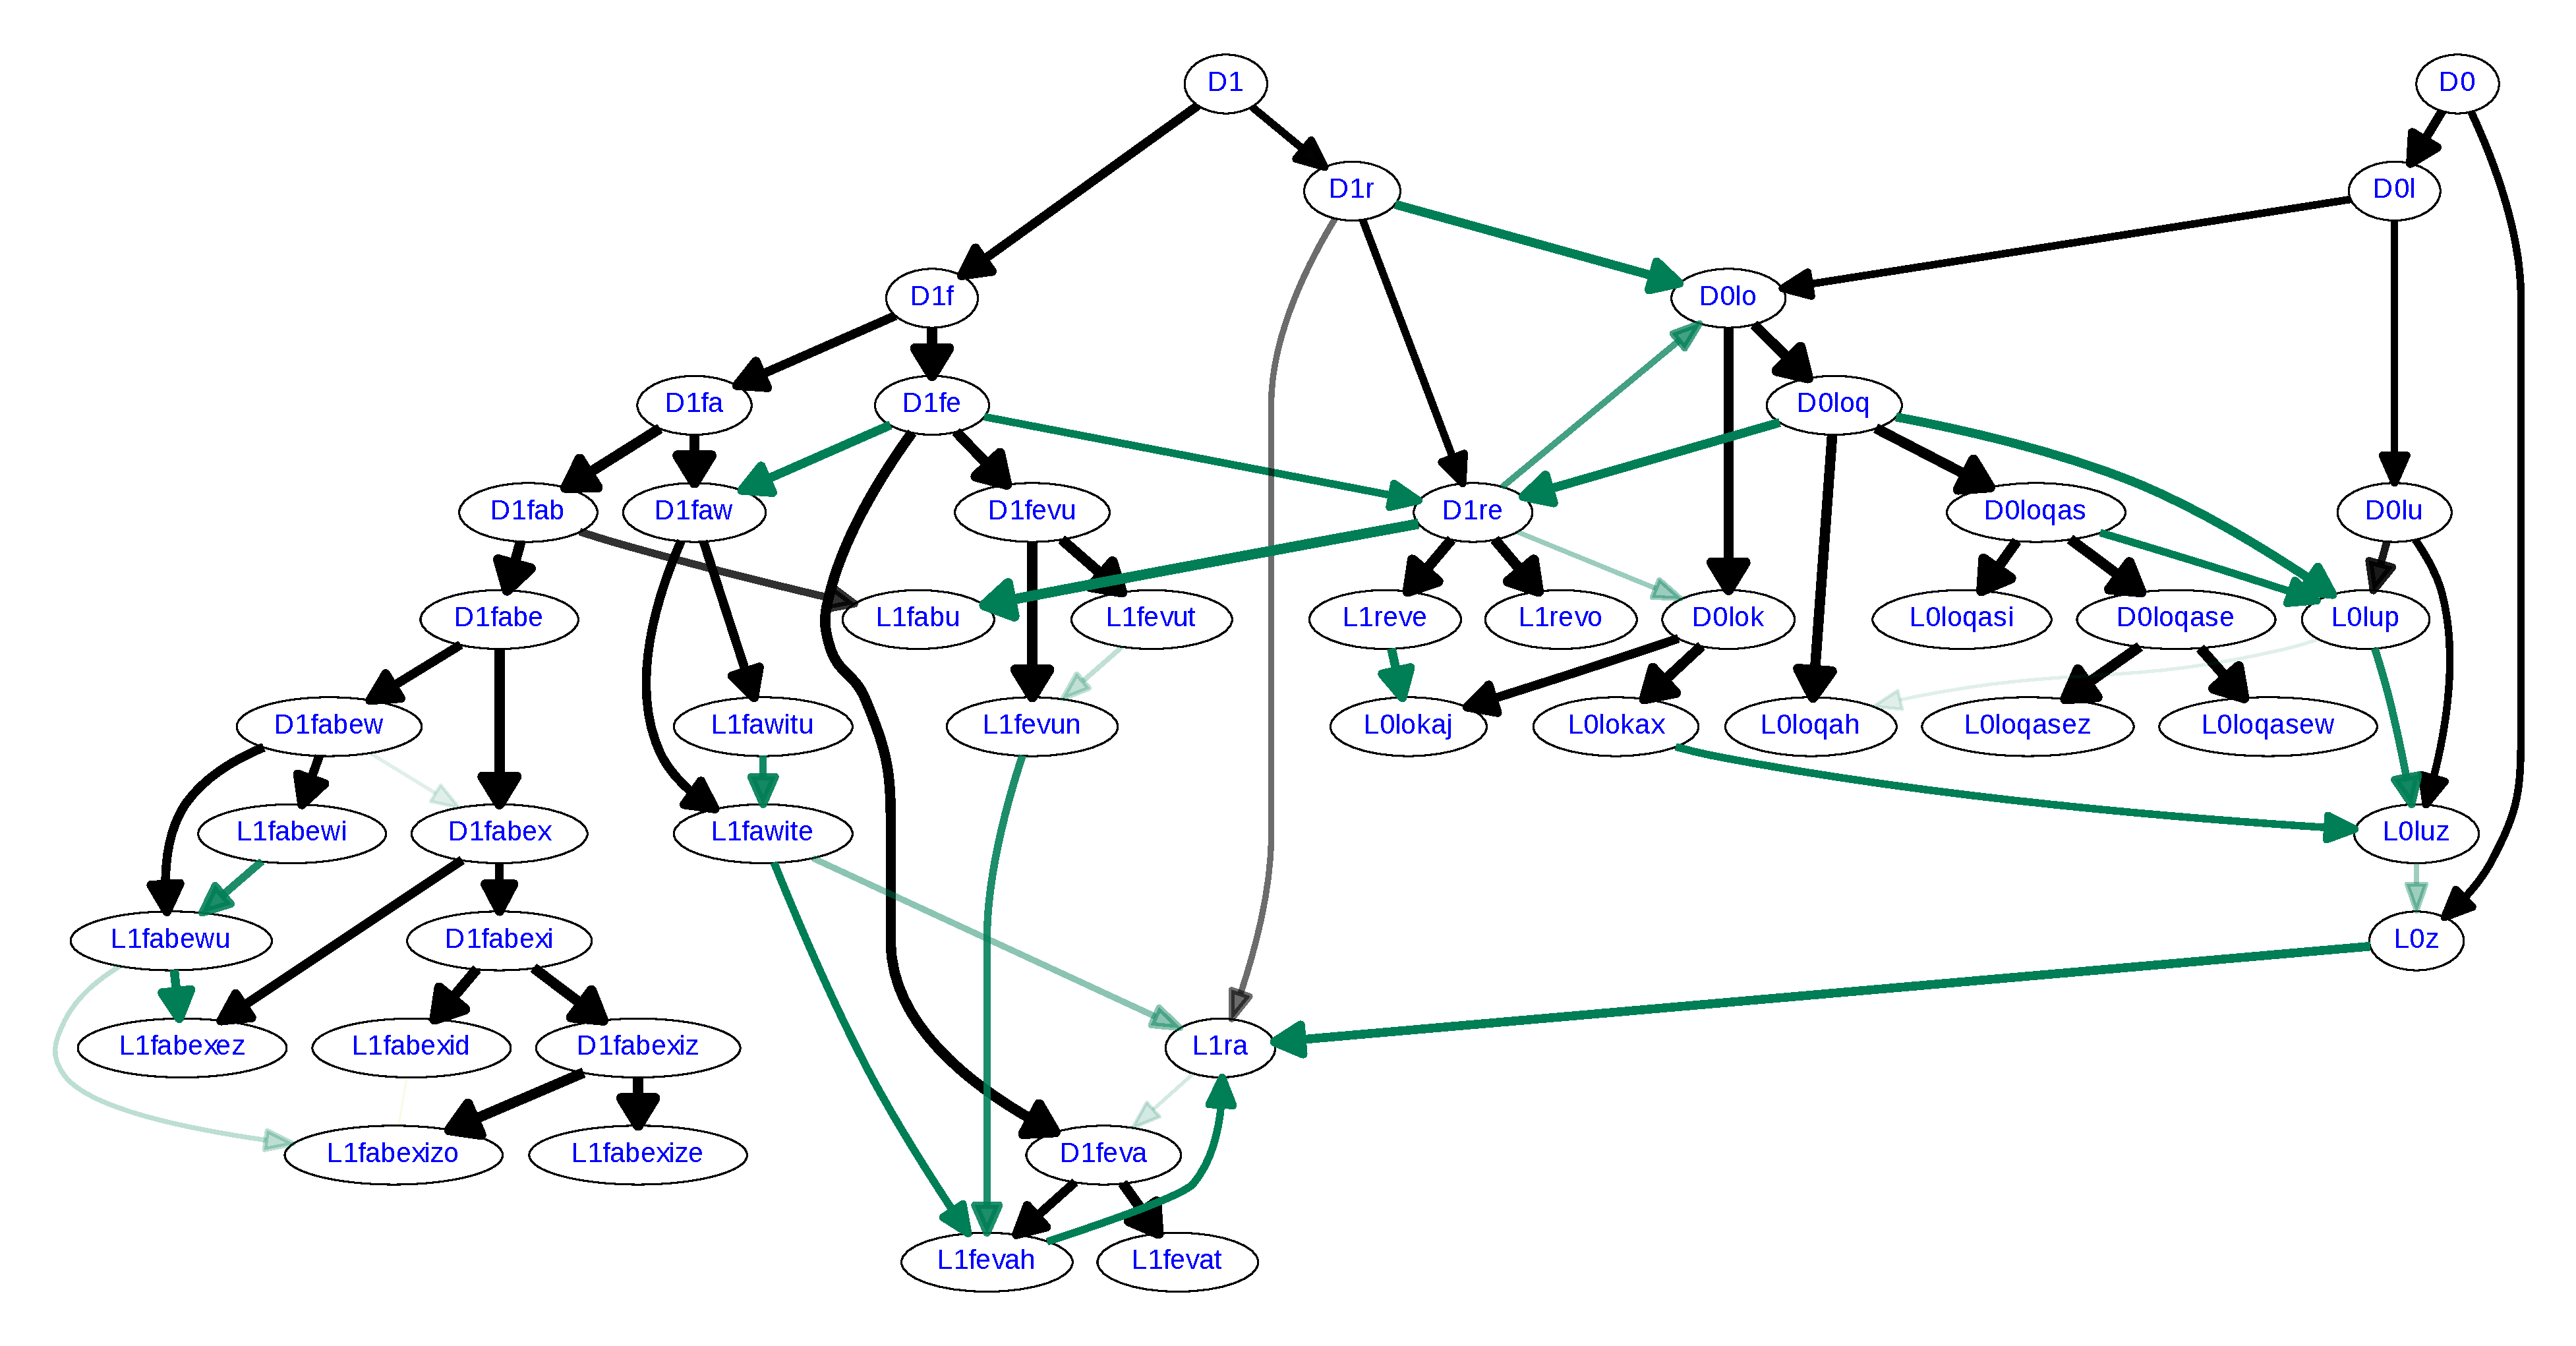
\includegraphics[width=\textwidth]{figures/sim-example-goldstandard-graph.pdf}
 \caption{An example of a simulated scenario, with complex interactions}
 \label{simulated-tree}
 \end{center}
\end{figure}

To showcase the geographic model, the maps in \figref{simulated-maps} shows the final positions of each language for the same scenario, as well as the state of the simulation after 1,800 and 3,400 simulated years (i.e.\ 3,200 and 1,600 years before the final state). The three maps give an impression of how the initial population splits to fill the available space, and what type of contact is simulated by the model. Open contact channels are visualized in dark green (monodirectional contact) and light green (bidirectional, i.e.\ contact channels in both directions are open). The thickness of these lines represents the intensity of the contact, i.e.\ the rate at which lexical material is transmitted across each channel.

As in the cognate overlap maps used to visualize the shape of the inference problems in \chapref{sec:4}, the thickness of the black lines visualizes the strength of cognate overlaps between living languages at the respective point in time. In the comparison between the three stages, it becomes very obvious how some lines which were still strong thousands of years ago have faded into the background, reflecting the loss of similarity caused by lexical replacement.

\begin{sidewaysfigure}
\begin{subfigure}{0.25\hsize}
 \centering
 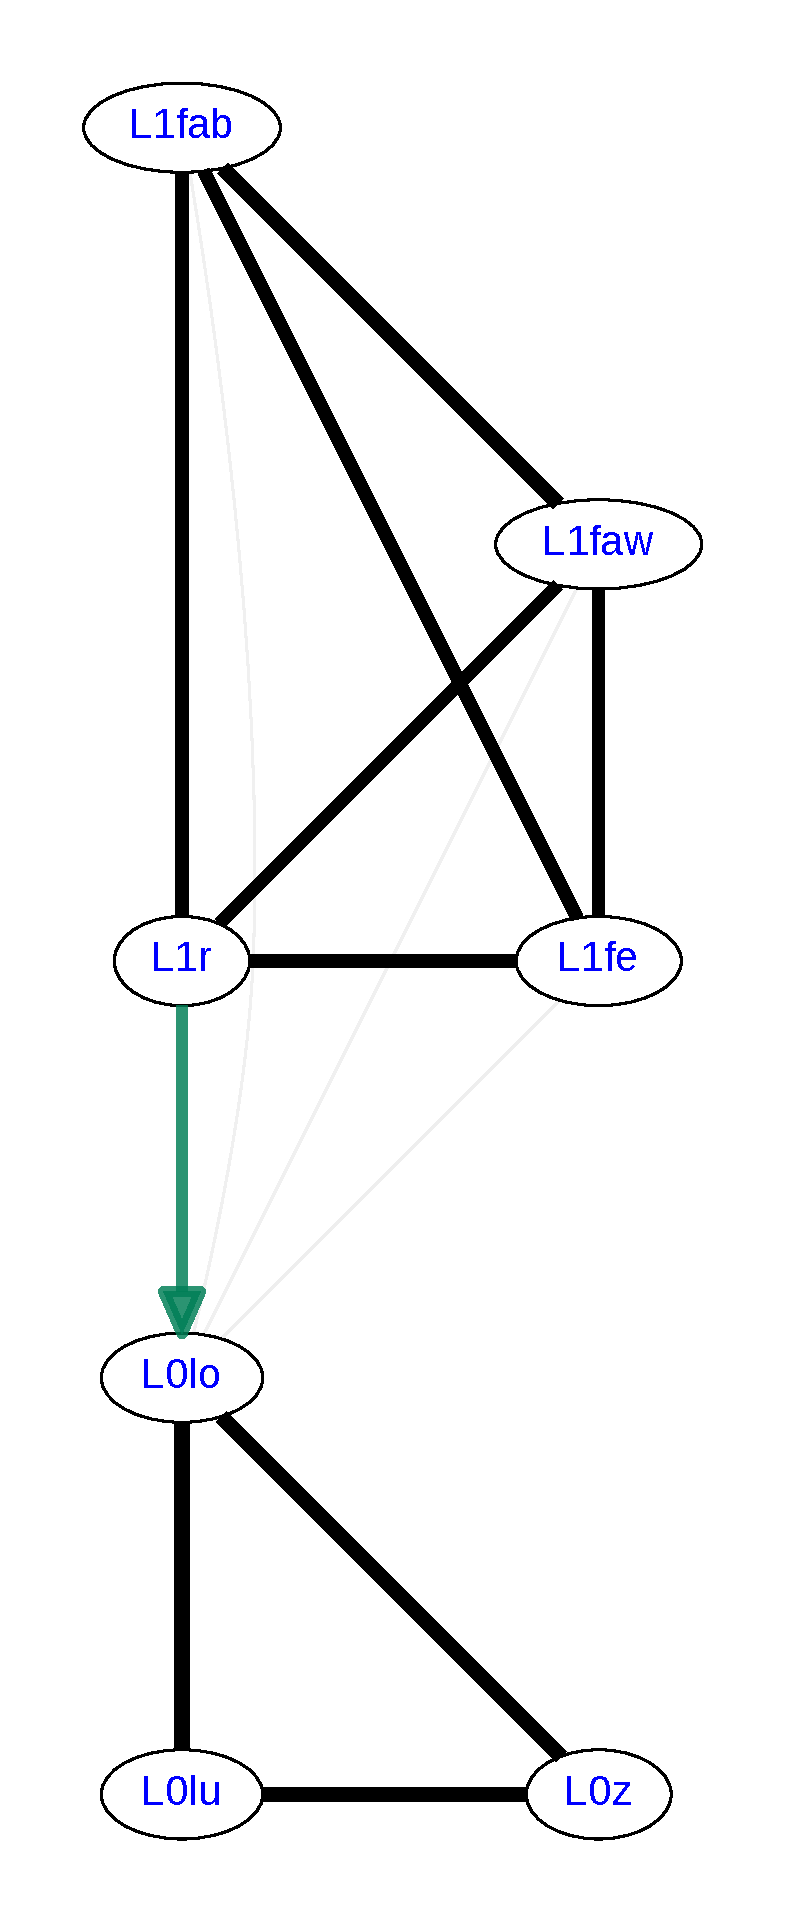
\includegraphics[scale=0.15]{figures/sim-example-initial-map.pdf}
 \caption{Situation after 1,800 simulated years.}
 \label{simulated-map-pastA}
\end{subfigure}
%
\begin{subfigure}{0.25\hsize}
 \centering
 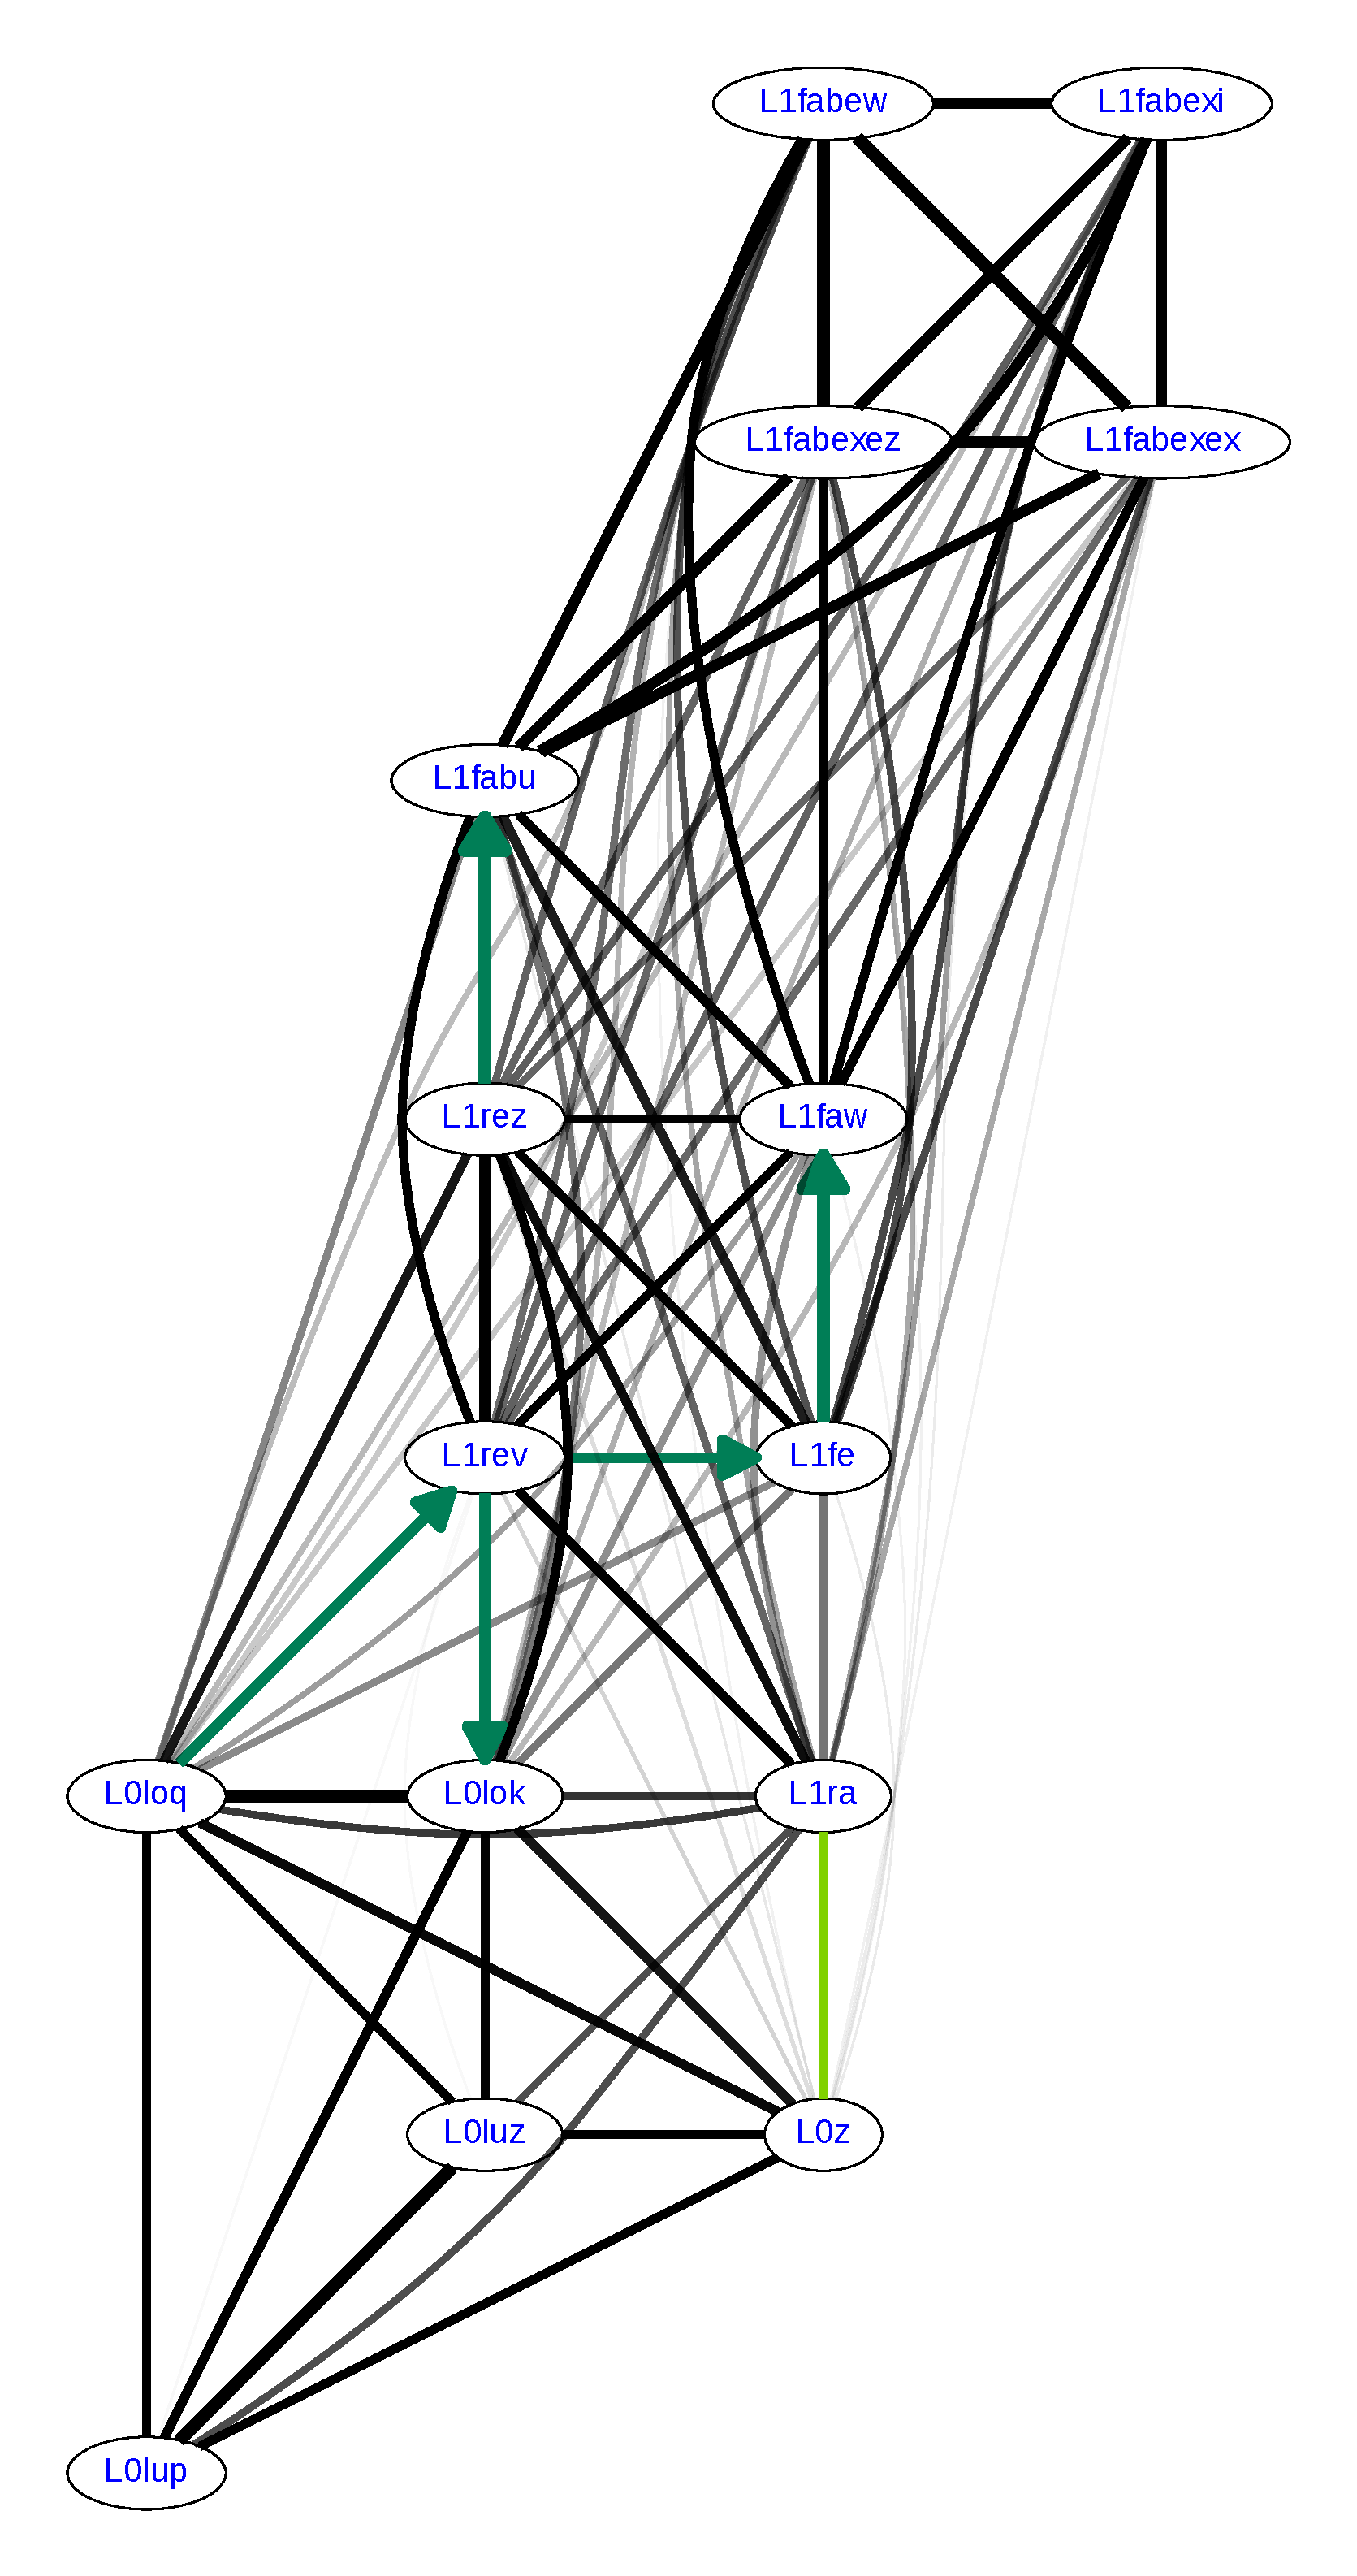
\includegraphics[scale=0.15]{figures/sim-example-past-map.pdf}
 \caption{Situation after 3,400 simulated years.}
 \label{simulated-map-pastB}
\end{subfigure}
%
\begin{subfigure}{0.4\hsize}
 \centering
 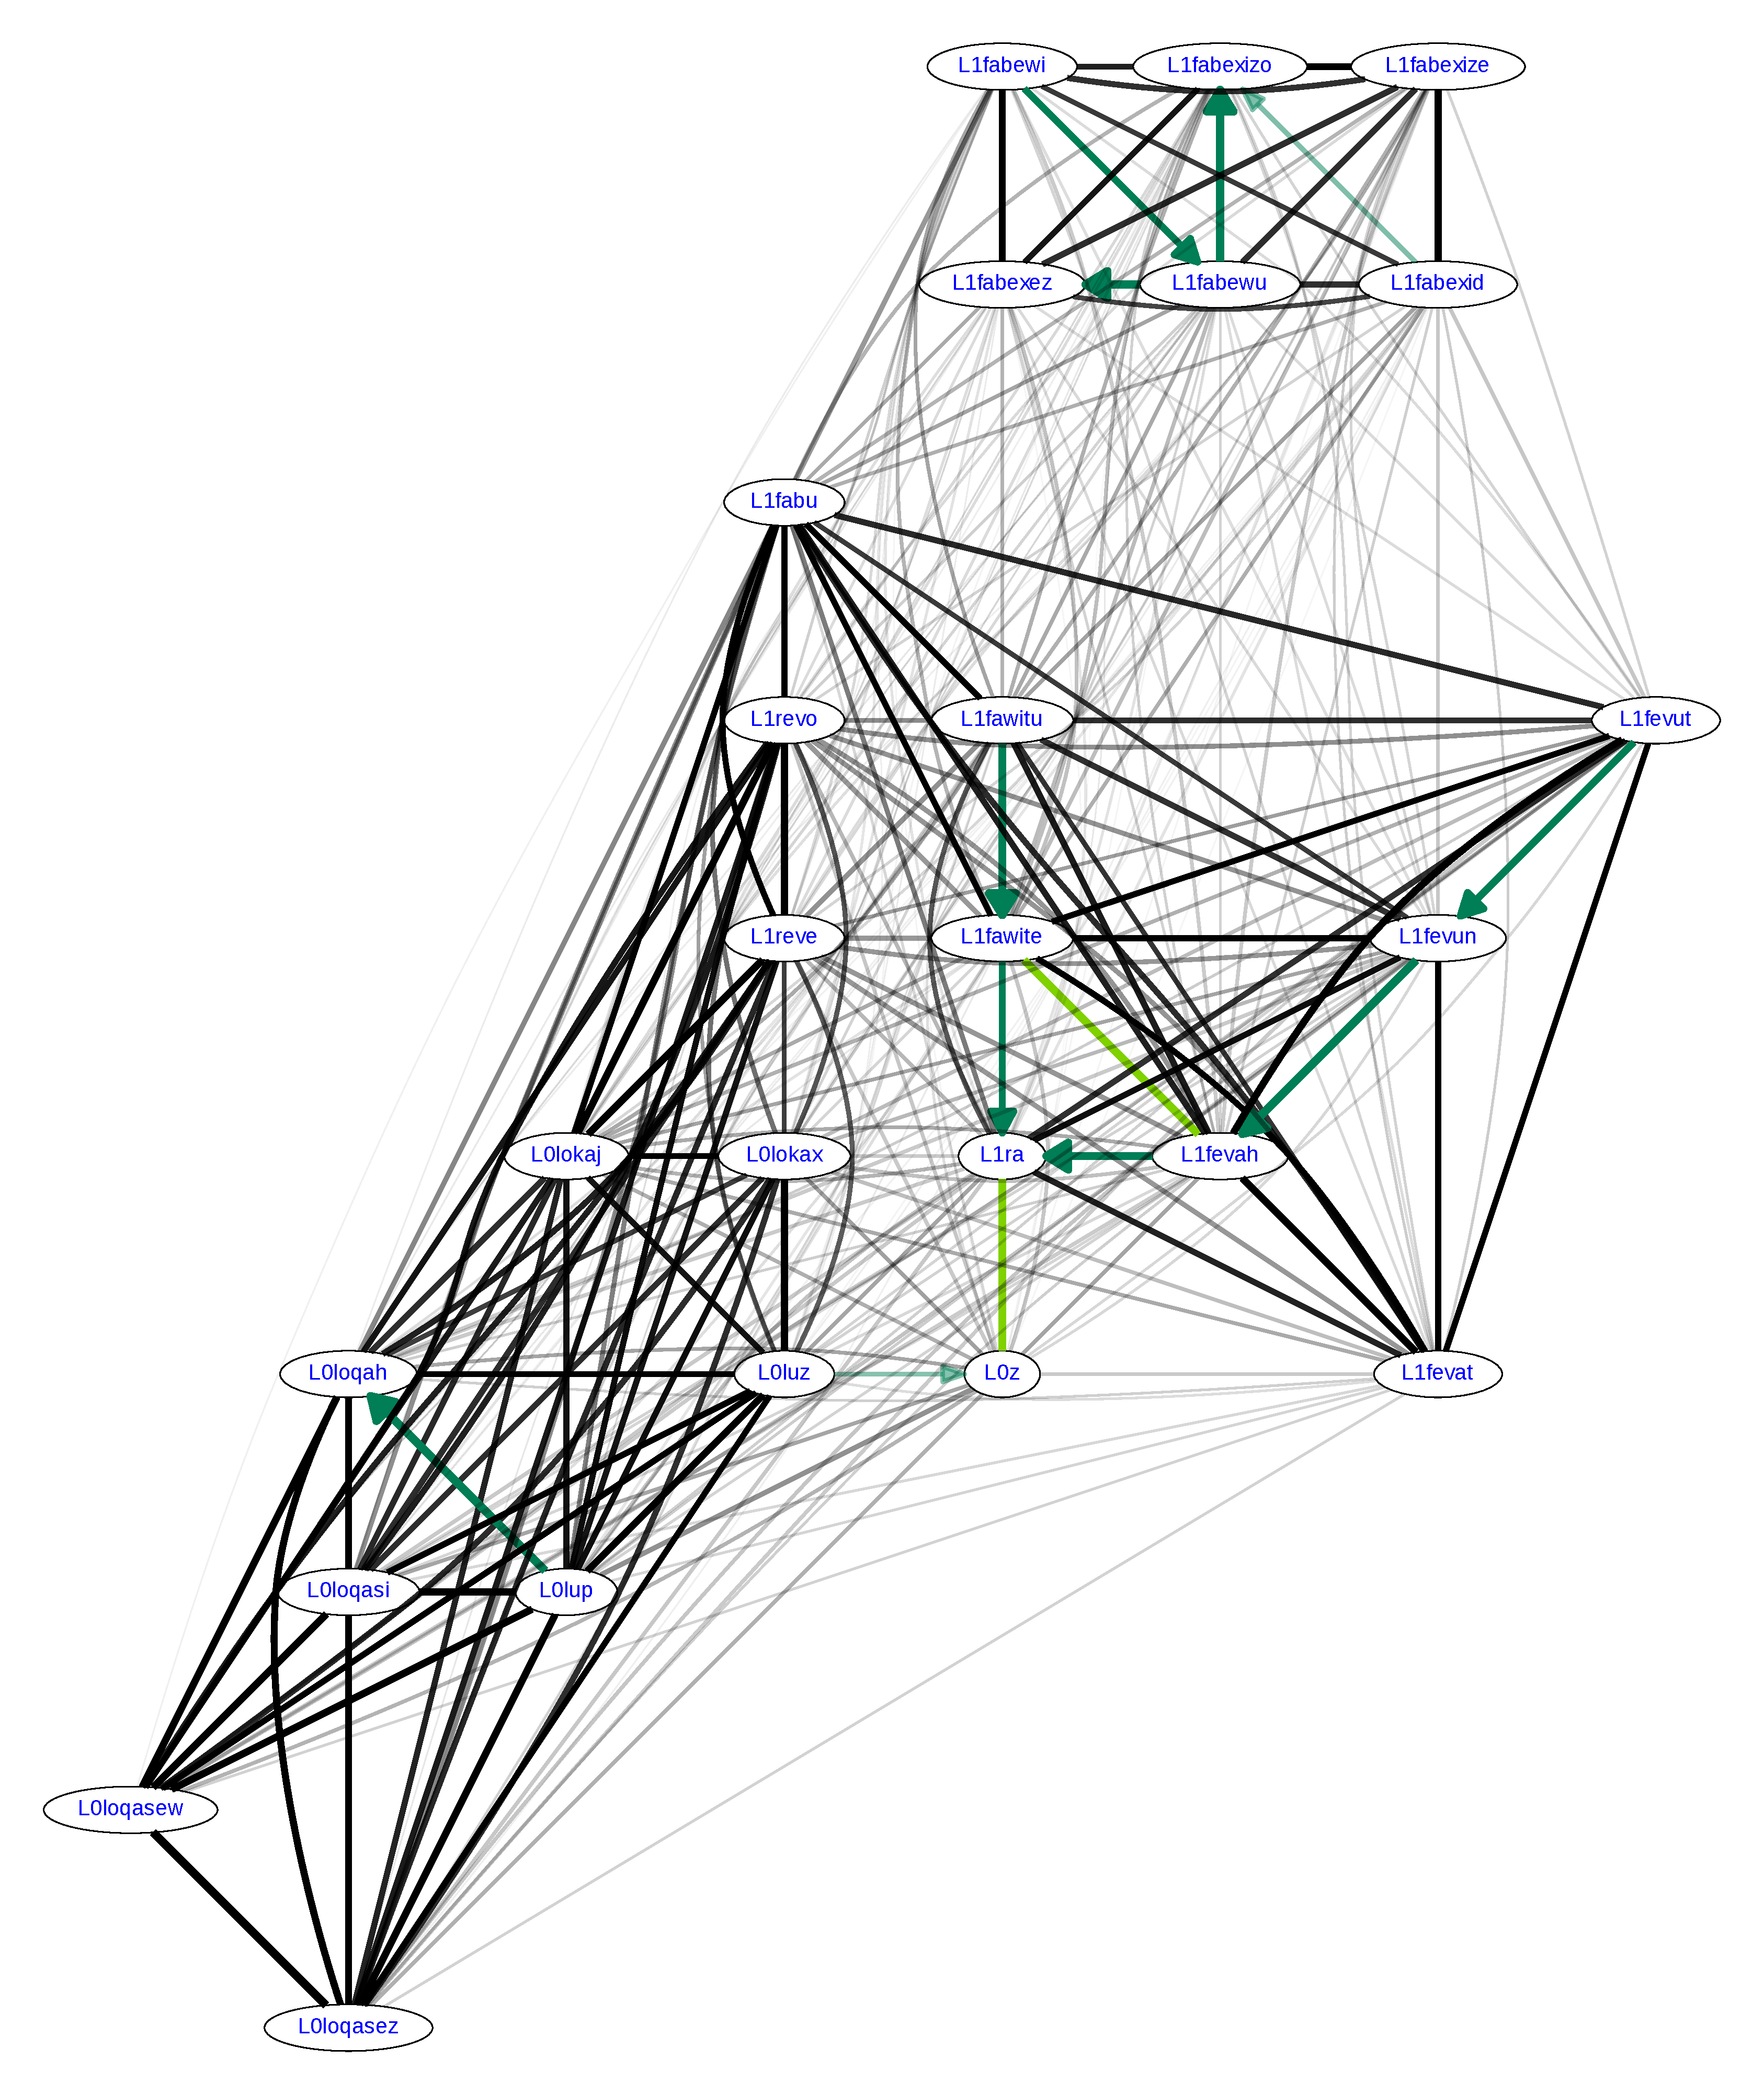
\includegraphics[scale=0.15]{figures/sim-example-present-map.pdf}
 \caption{Final situation after 5,000 simulated years.}
 \label{simulated-map-present}
\end{subfigure}
 \caption{Maps visualizing the situation of the example scenario at three points in time}
 \label{simulated-maps}
\end{sidewaysfigure}

To generate the evaluation set, a total of 50 scenarios were generated by simulation. Taken together, the simulated data contain 2,139 living languages distributed over 297 language families. In addition, a total of 7,128 intermediate (proto-)languages was modeled while producing the data for the living languages. In total, while generating the history of the languages, a total of 2,250,891 borrowing events were generated and logged, of which 380,571 events (16.9\%) turn up in the stored etymologies of one of the 2,139,000 lexical items in living languages.

In order to decide in which respects the simulation model does make sense (or not), the next section addresses the question whether the simulated data are similar enough to the NorthEuraLex data to be able to serve as additional test cases for validating my results. The section thereafter will answer the question whether the generated histories are non-trivial enough to provide some challenge to phylogenetic and lexical flow inference methods, and also varied enough to cover a wide array of situations we would expect to be faced with in actual linguistic histories.

\subsection{Are the scenarios realistic?}
The most trivial question to ask about the realism of the simulated histories is whether the distribution of cognate class sizes is similar enough to the one inferred from the NorthEuraLex data. The average size of cognate sets in the NorthEuraLex data is 2.253, whereas the simulation produces scenarios with average cognate sizes $2.164 \pm 0.192$, with the maximum being $2.656$, and the minimum $1.801$. This shows that the simulated cognate sets are similar in the size to the ones inferred by NorthEuraLex, indicating that the types of overlaps and therefore the information geometry will behave similarly. But since the average size of cognate sets heavily depends on the number of languages in the dataset, it might be more relevant to compare the average number of cognate sets per concept per language, and compare this measure across scenarios. In the simulated data, this number varies around $0.577 \pm 0.095$, with the minimum at $0.388$ and the maximum at $0.800$. The equivalent measure computed from the 
inferred correlate sets in NorthEuraLex is $0.497$, again fitting very well into the distribution of simulated scenarios. Finally, \figref{cognate-class-sizes} shows the distribution of cognate class sizes in the simulated data next to the one for the classes automatically inferred from NorthEuraLex. It is clearly visible that both distributions are very similar, except for a much higher ratio of two-element cognate classes resulting from automated cognate detection. This fits well with the observations made when inspecting the inferred classes for \textsc{fish}, and is very likely an artefact of UPGMA clustering, which is sensitive to spurious pairwise similarities between elements which should form singleton classes. This difference also becomes visible when fitting Pareto distributions to the observed counts. The maximum likelihood estimates of the alpha parameter are $\alpha = 0.284$ for the NorthEuraLex data, but only $\alpha = 0.189$ for the simulated data. 

\begin{figure}
 \begin{center}
 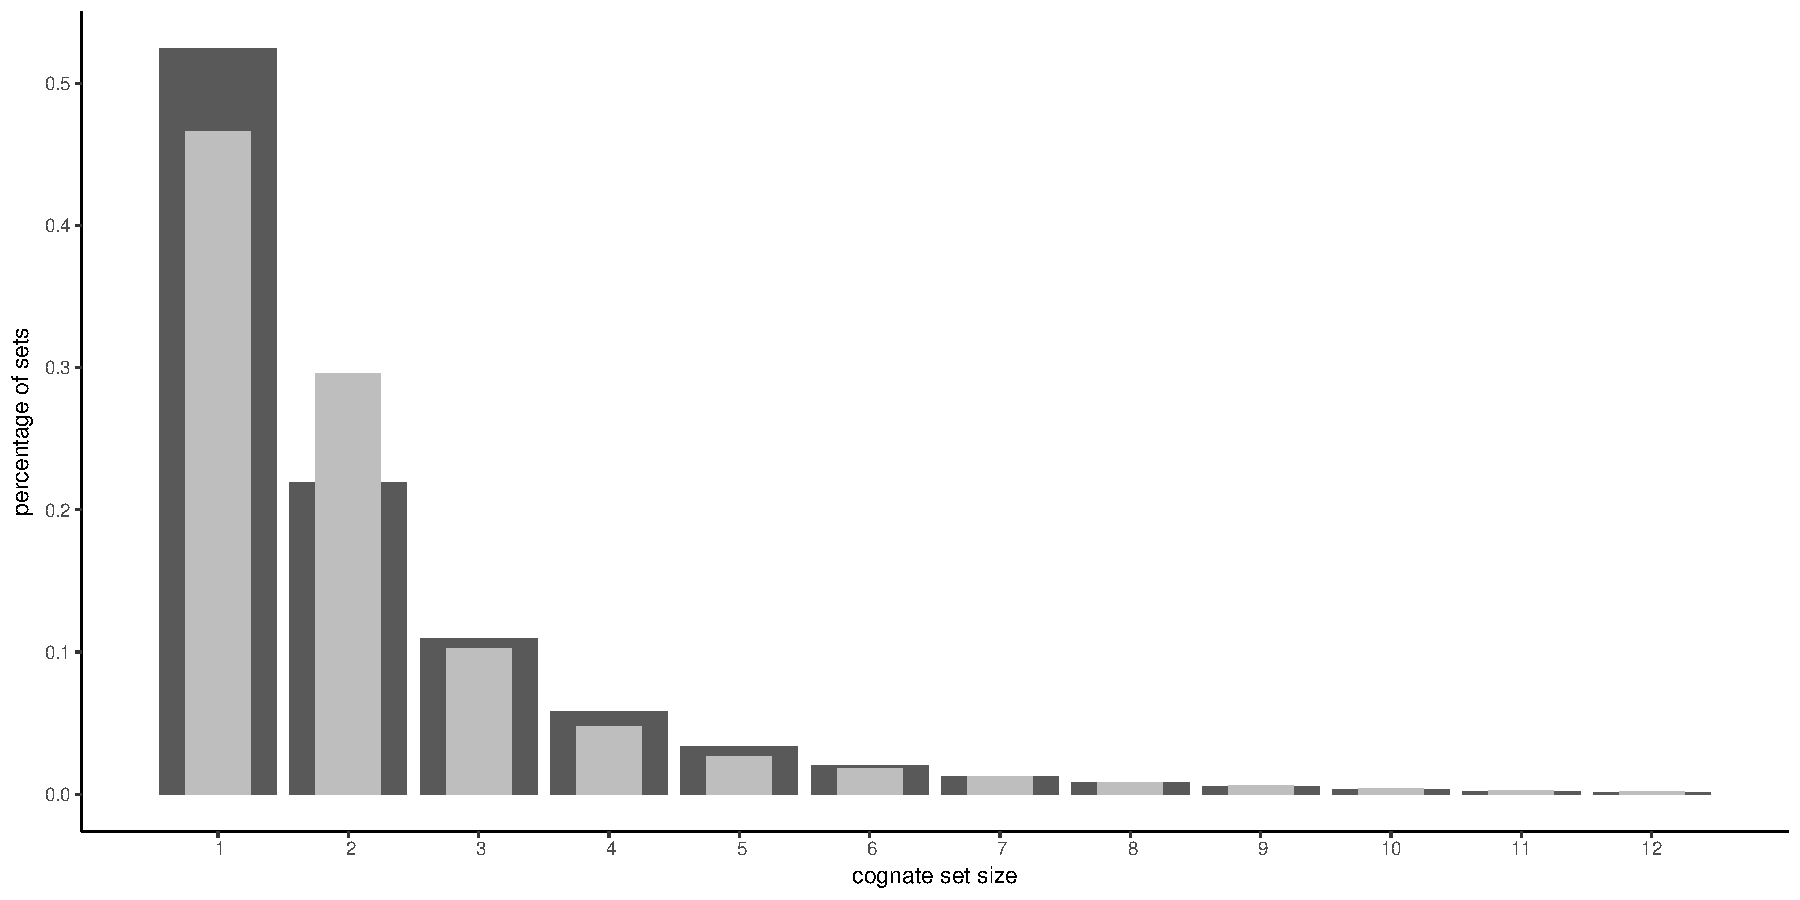
\includegraphics[width=\textwidth]{figures/cognate-set-sizes.pdf}
 \caption{Distributions of cognate class sizes on NorthEuraLex (gray) and simulated data (black)}
 \label{cognate-class-sizes}
 \end{center}
\end{figure}

To get a first impression of how realistic the amount of contact in the simulated data is, we can compute the percentage of words in the final data which were borrowed at some point in their history. Across all scenarios, 23.92\% of all attested words have at least one borrowing event as part of their history. Between scenarios, the ratio varied between 1.27\% and 38.53\%, with the mean at $23.07 \pm 8.71\%$. This is very much in line with the numbers derived from the WOLD database and summarized in \cite{tadmor2009}, where the ratio of loans in content words varied between 1.3\% (\ili{Mandarin Chinese}) and 65.6\% (Selice \ili{Romani}), and the average ratio of loans across all languages was $24.2\%$. Therefore, both the overall frequency of loans and the variance of the ratio across simulated languages and scenarios are very realistic.

With respect to lexical replacement, we can compute the distribution of word ages from the logged histories. For each word in a living language, we can trace back the history to the point where the word came into existence as a word for the concept in question by a replacement event (a mutation, in biological terms), or back all the way to one of the initial languages. Across all scenarios, 16.93\% of the words could be traced back to one of the initial languages. Unsurprisingly, the distribution almost exactly fits an exponential curve with our loss rate of about 0.036\% per year, leading to e.g.\ 3.42\% of words older than 4,500 years, 6.83\% between 2,000 and 2,500 years old, and 16.29\% younger than 500 years. The language-wide averages of word ages were distributed around $2357.43 \pm 133.84$. I have found it impossible to find even rough cross-linguistic estimates for the word age distribution across entire lexica of modern languages. Still, we can use some etymological resources to get a first 
impression whether the numbers seem realistic. \cite{sammallahti1988} provides the most up-to-date overview of the known lexicon of Proto-Uralic\il{Uralic languages} as well as some later proto-languages of branches such as Finno-Ugric\il{Finno-Ugric languages}. He counts 124 Uralic stems as being reconstructable for Proto-Uralic (perhaps 7,000 years ago), about 290 additional ones for Proto-Finno-Ugric (5,000 years ago), and 150 more for Proto-Finno-Permic\il{Finno-Permic languages} (a contested subgrouping of perhaps 4,000 years). \cite{janhunen1977} reconstructs about 700 stems in total for Proto-Samoyedic\il{Samoyedic languages}, at about 2,500 years of age. A typical dictionary of a fully known language that is sorted by lexical roots, such as \cite{de_vaan_2008} for \ili{Latin} or \cite{lehtisalo_1956} for \ili{Nenets}, covers the history of about 2,000 roots. We can thus assume that this is roughly the number of etyma which we can assume for an unwritten language. Fitting an exponential curve to these 
five data-points, our replacement rate of 0.036\% per year, or about 30.24\% per millennium, fits almost perfectly. Calculating the distribution of word ages across this curve (and counting every word older than PFU as 5,000 years old in the same way as I need to do it for the simulated data), we arrive at a mean age of $2317.5$ years, which again fits very well into the distribution of values derived from the simulated data. The distorting effect of borrowings on reconstructability therefore seems to have a very negligible influence.

Another interesting question to ask about the distribution of word ages is whether there are conservative languages which tend to conserve more ancient words across the basic lexicon, whether due to limited lexical contact, or an inherent tendency to slower lexical replacement. This is equivalent to the question whether different languages can have vastly different average replacement rates across a timescale of thousands of years. While there is considerable evidence that replacement rates can vary a lot on the short term \citep{atkinson_ea_2008}, it is unclear whether these differences are random fluctuations which might equal out with time, or whether they are inherent properties of language systems which remain in place for millennia. On the simulated data, while the underlying model of divergence operates at a global replacement rate for all languages, replacement by borrowing leads to very different retention rates. In the most conservative simulated language, the average word age was $3475.92$, as 
opposed to $1892.89$ in the language with the least stable vocabulary. This shows that a mixture of a variance in global replacement rate for each scenario already leads to an interesting and realistic range of measurable conservativity in the simulated languages.

The next relevant point of comparison is the shape of the trees. An essential observable property of binary trees is their balancedness, which can be defined in many different ways, each capturing a different type of asymmetric behavior. \cite{holman2005} analyzes linguistic trees in this framework, making the very interesting observation that language trees have different structure than would be generated by simple birth and death processes, even if we allow different diversification rates for each branch. Holman uses the weighted imbalance score by \cite{purvis_ea_2002}, to show that actual language trees are much more unbalanced than such a model would predict. The imbalance score for a binary node $l$ with children $l_1$ and $l_2$ is computed as $I(l) := \frac{B - \lceil S/2 \rceil}{S - \lceil S/2 \rceil - 1}$, where $S$ is the number of nodes on the subtree under $l$, and $B$ is the maximum of the sizes of the two subtrees under $l_1$ and $l_2$. $I(l)$ will be 0 for a maximally balanced node (in the 
sense that a node with this number of descendants could not be more balanced), and close to 1.0 if one of the children is a leaf and many other nodes are descendants of the other child. For an entire tree, the \isi{weighted imbalance score} is a weighted mean over these node-based scores, where the weight $w(l)$ is $1$ if S is odd, $w = (S-1)/S$ if S is even and I > 0, and $w = 2(S-1)/S$ if S is even and $I = 0$ (such that completely balanced nodes count twice). This score is defined in such a way that the expected value for trees generated by a birth and death process is 0.5. As Holman shows, the weighted imbalance scores for actual language trees are significantly higher than that, clustering around 0.7. The simulated trees have weighted imbalance scores between $0.587$ and $0.820$, with the mean at $0.698 \pm 0.053$, which fits Holman's results surprisingly well. It seems that a simple death-by-replacement model on a constrained geography is all that is needed to explain the imbalance in empirically 
observed trees, without any need to allow for branch-specific diversification rates or similar devices.

There are some additional phenomena which are so commonly observed in historical linguistics that realistic datasets should contain some instances of them. One of these are isolates\is{isolate}, which can here simply be defined as phyla with only one surviving descendant language. According to the Glottolog classification, roughly half of the world's families are isolates, and this is also roughly the ratio of isolates in NorthEuraLex (9 out of 21 families). While isolates are not interesting for evaluating phylogenetic methods, they can still be involved in some interesting contact scenarios, and should therefore be present at least in a few scenarios. So does the simulation model, where isolates can only occur if one of the initial languages never splits during 5,000 simulated years, or if all but one of the potentially many languages from a family are replaced by neighboring families branching and expanding into its territory, produce a significant number of isolates? Across all scenarios, only 16 of the 
270 families generated by the simulation model are isolates, a number which is unrealistically low compared to the large numbers of isolates we observe in many regions of the world. While this is not a problem for evaluation purposes (as long as some isolates are present), it might still be worthwhile to speculate why so many more isolates occur in reality. One possible explanation is that the over-simplified geography (without remote mountain valleys) does not generate enough niches for smaller families to survive. Moreover, the constraint of having exactly one language per place will counteract the arising of true isolates. In reality, if two villages with closely related dialects of an isolate are surrounded by completely unrelated languages, the two villages might prefer close contacts among each other, counteracting the divergence into separate languages.

As a final point, a problem of realistic complexity should contain substrates. To recapitulate, a substrate relationship is one possible result of language shift, when the speakers of one language rapidly shift to another language, but the shift is incomplete in leaving traces of the ancestral language (a substrate) in the new language. In historical linguistics, the term \textit{\isi{substrate language}} is often used in the sense of an otherwise unattested language whose existence can only be reconstructed from a layer of words which have no etymology in the respective family. With access to the simulated history of each word in a large datastructure, it becomes possible to compute the ratio of words which were borrowed at some point from a substrate language, and the number of languages without living descendants which became sources of such borrowings. Analyzing the histories of all words in the simulated dataset, we find that 5.04\% of all words have a substrate history by our definition. Averaging 
across scenarios, $65.16 \pm 37.05$ languages, i.e.\ slightly less than half of the $142.56 \pm 62.66$ extinct languages, played the role of a substrate language during the history of at least one word. Of $78.62 \pm 37.41$ contacts, $26.14 \pm 17.24$ occur with a donor language which leaves no living descendant in an average scenario. It is difficult to assess how realistic these numbers are, because in the real world, words without an etymology are often difficult to attribute to one common substrate donor. Still, there tend to be many instances of unknown substrates even in the history of a very limited linguistic region such as Northern Europe. The most famous instance is an unknown substrate in Germanic\il{Germanic languages} consisting of mainly maritime vocabulary such as \textit{*strand\={o}} `beach' and \textit{*seglan} `sail'. Originally assumed to comprise a third of the common Germanic lexicon, it has been shrinking in size as additional Indo-European etymologies for Germanic lexemes are being 
established. While some scholars like \cite{hawkins1990} continue to advocate it, it now seems to be on the way to becoming a minority position. Less contested instances of substrates in the North are a layer of pre-Uralic lexical material in the \ili{Saami languages} \citep{aikio2004}, and a different pre-Uralic substrate which heavily influenced the \ili{Samoyedic languages} \citep[e.g.][]{helimski1998}. Given the ubiquity of such examples even in an area with a rather short post-glacial settlement history, it makes sense to have substrate relationships occur so frequently in the simulated data.

\subsection{Are the scenarios interesting?}
The second question about the adequacy of the simulation model is whether the simulated scenarios are difficult and varied enough to make the results of evaluation interesting. To answer the first question, this section analyzes how well the tree signal is recoverable from the overlap of cognate classes alone, and, answering the same question from a slightly different angle, how well the cognate class boundaries coincide with phylogenetic units. Then, the identifiability of contact events is analyzed in order to quantify the maximum performance that we could hope an ideal system to achieve on the lexical flow inference task. For an answer to the second question, the section goes through some phenomena that we might expect to occur in actual linguistic histories of geographical areas where several language families are neighbors for several millennia, and discusses to what extent these phenomena also occur in the simulated data.

A very direct way of assessing the difficulty of phylogeny inference is to measure the recoverability of the tree signal from the cognate data. If the cognate overlaps perfectly encode the tree structure, we should have $|c(A,B)|$ > $|c(A,C)|$, $|c(B,C)|$ in all configurations where $A$ and $B$ are more closely related than either is with $C$, or more precisely, if the lowest common ancestor of $A$ and $B$ is a descendant of the lowest common ancestors of $A$ and $C$ as well as $B$ and $C$. In the simulated scenarios, the cognate overlaps match the criterion for $89.32 \pm 6.87\%$ of such triples. On the automatically inferred cognates derived from NorthEuraLex and the reduced Glottolog tree, the value is $82.28\%$, i.e.\ comparable in complexity to the more difficult simulated scenarios. In the most difficult scenario, the inequality only holds for $64.91\%$ of triples, and the easiest scenario (with only one contact in 5,000 years) has $100\%$. Given the presence of errors in automated cognate judgments, it is hardly surprising that the NorthEuraLex task is on the more difficult end of the scale.

A more strict measure of the difficulty of the inference task is the fit of cognate set boundaries to phylogenetic units. More precisely, we are interested in the percentage of cognate sets which exactly correspond to the descendants of a single phylogenetic node. Note that this correspondence is not only destroyed by borrowing, but also by lexical replacement in one language of the unit, though the latter situation will produce a new cognate set which is aligned to a phylogenetic unit of trivial size. On the simulated scenarios, the distribution of this percentage can be summarized as $17.33 \pm 4.98\%$. The value of $10.06\%$ on NorthEuraLex cognates and the Glottolog tree is close enough to this distribution to provide additional evidence that the simulated scenarios are quite realistic in difficulty. However, the NorthEuraLex data are by this measure more challenging even than the worst of 50 simulated scenarios at $10.28\%$. This is again easily explainable by the existence of erroneous automated 
cognacy judgments, as both false positives and false negatives will destroy perfect alignments of cognate classes with phylogenetic units. On the tree signal, the errors apparently almost cancel out, not detracting much from recoverability, whereas the matches of entire cognate sets are much more sensitive to uncertain cognacy judgments. This has problematic implications for algorithms building on cognate set overlaps, such as the lexical flow inference procedure I will be exploring.

An important question to ask about the data concerns the identifiability of contact events. How many of the contact channels still have visible consequences in the living languages, in the sense that they are part of the histories of enough words in living languages to go beyond the detection threshold of 20 loans? This measure gives us an upper bound on the performance we could hope to achieve with any algorithm which reconstructs previous reflexes of cognate sets and then tries to infer contact events. In the simulated data, 67.6\% of all simulated contacts were still visible by this definition, resulting in an average of $49.68 \pm 23.16$ detectable contacts per scenario. This number implies that certainly enough interesting contact patterns occur in the simulated data, and the consequences of two thirds of these are still in principle detectable in the output data.

Finally, a few words can be said about the variability of patterns encountered in the simulated data. Using graph terminology, there are 27,164 unshielded triples in the gold standard flow graphs. 15.05\% of these are colliders, where a single language is influenced by two different languages. 550 (13.45\%) of these colliders connect languages which have not interacted in any way before. As we will see in the next chapter, this type of collider is easily detectable using v-structure tests, giving us very reliable directionality information. The problem is that out of 12,179 lateral connections whose directionality we will want to determine, only 870 take part in such strict colliders, and 4,088 lateral connections are part of any type of collider. This means that we only have completely reliable directionality information for 7.14\% of these connections, and some direct evidence for 33.6\%. The directionality of two thirds of our lateral links would thus have to be determined by some form of constraint 
propagation, which will cause some problems if our unshielded collider tests are not completely reliable. To sum up, the simulated instances are definitely challenging enough to provide useful information about the potential of causal inference for lexical flow inference.

Coming to phenomena of more immediate linguistic interest, we first consider chains of loans, where lexical material is transmitted from one language to another through a third language which serves as a bridge, whereas the first two languages are not directly in contact. Such chains would mirror the phenomenon of wanderw\"orter such as \textit{sugar} or \textit{wine}, which were not borrowed from one original language into every language which now uses them, but travelled from language to language together with the trade goods, reaching remote geographical areas via trading intermediates. In the simulated data, 16.4\% of words with a borrowing history were borrowed twice, and 2.9\% were borrowed three or more times. There is thus a fair amount of wanderwort-like word histories in the data, adding to the realism of the simulated scenarios.

Another phenomenon whose frequency is worthwhile to investigate is \isi{internal borrowing} within the same language family, i.e. the situation in which a word can be replaced by a cognate word. In the simulated data, because related languages are more likely to be neighbors, internal borrowing happens quite often, so that in $26.280\%$ of all generated borrowing events one cognate set was replaced by the same set, not changing anything about the data. Across scenarios, this percentage was pretty stable at $29.531 \pm 5.80\%$, although there are some outliers with the maximum at $67.3\%$. Set-internal borrowings are obviously a problem for contact detection algorithms which work on the level of cognate sets, because such borrowings do not leave any detectable traces.

\section{Potential further uses of simulated scenarios}
In addition to their usage as test cases for evaluating my methods, other researchers might want to use simulated scenarios as generated by my model as well. For instance, because each event during the simulation is logged in a format which allows the complete history of each word to be tracked explicitly, it becomes possible to evaluate loanword detection algorithms on much larger datasets than the real datasets which are currently and will ever be available.

This also applies to the comparative evaluation of methods and algorithms for tasks wich are closely related to lexical flow inference, such as the inference of different types of phylogenetic networks. In this context, the simulation could be used to assess the impact of lateral transfer on the reliability of phylogenetic inference methods, e.g.\ for practical experiments reinforcing the empirical findings by \cite{greenhill_ea_2009} or the mathematical results of \cite{roch_snir_2012}, both indicating that phylogenetic inference is quite robust to realistic amounts of lateral transfer.

For all these purposes, the simulated scenarios are distributed together with this book in various standard formats (trees in Newick format, cognacy data in a Nexus format readable by the most common software tools in phylogenetic inference). Moreover, my Java programs for generating more scenarios of this type, as well as the parsers for the log files which are necessary to extract statistical information of the type I was covering in this chapter, will be packaged and released as standalone executables along with their source code in order to allow other researchers to adapt the simulation model to their requirements, or experiment with different parameter settings than the ones I have been operating on here.

\chapter{Phylogenetic lexical flow inference}
In many respects, this chapter represents the core of this book. It discusses both the idea of and the methodological difficulties in applying causal inference to data in the shape of overlapping cognate sets in detail, before defining PLFI (phylogenetic lexical flow inference), the first of two algorithms I describe in this book, and then evaluating it on both NorthEuraLex and the simulated scenarios.

This algorithm requires adding reconstructions of all known proto-languages to the model, which makes it causally sufficient, allowing me to work with the much simpler PC algorithm, and postponing the need to get into the complexities of the RFCI algorithm to the next chapter.

In Section 6.1, I discuss possible ways of modeling lexicostatistical data as statistical or information-theoretic variables, and motivate my decision to stick to coarse-grained cognate overlap judgments for the purposes of this book. Section 6.2 then introduces my cognate-based information measure, which allows me to derive a very natural measure of conditional mutual information between languages in Section 6.3.

Sections 6.4 and 6.5 are concerned with ways to specialize parts of the PC algorithm in order to balance out assumptions that are not met by conditional independence tests based on this measure. These include the development of an explicitly flow-based criterion for defining plausible separating sets, and of two heuristic criteria for aggregating evidence of directionality. These criteria become necessary because the separating set membership criterion of the PC algorithm is found to be too unstable on cognacy overlap data.

Section 6.6 describes how I arrived at the guide tree for my experiments on NorthEuraLex, which is then used in Section 6.7 to perform ancestral state reconstruction in order to create the data for the proto-languages. Before deciding on maximum-likelihood construction as the basis of the PLFI algorithm, I evaluate several alternatives on the simulated data from Chapter 5.

Section 6.8 then puts the results of the previous sections together to define the PLFI algorithm, which is finally evaluated in the last section of this chapter, both on the NorthEuraLex gold standard developed in Chapter 4, and the simulated data from Chapter 5.

\section{Modeling languages as variables}
Everything starts with the idea of detecting conditional independence relationships between sets of languages, making it possible to apply causal inference algorithms to the lexical flow inference task. To take up the idea foreshadowed by the language examples in Chapter 3, I will assume the lexicon of each language to quite literally be caused by the lexicon of its ancestor language and possibly other languages which influenced its development. Put differently, the model is intended to determine how the lexicon of a language came about as a mixture of lexical material from other languages, and summarize the results in a causal graph.

As the crucial step towards this goal, we need a formalism which makes it possible to treat languages as information-theoretic variables. Depending on a range of choices about how we model languages, there are many possibilites to define useful measures of information content and mutual information between languages. While a single rather simple measure on cognate sets will be used later, in this section the idea will be put into a wider context by discussing more generally the different ways in which languages might be treated as statistical or information-theoretic variables.

\subsection{Languages as phoneme sequence generators}
The reductionist premise of lexicostatistical databases is to view each language simply as a (possibly many-to-many) mapping from concepts to lexical realizations. This means we could treat languages as variables generating sequences of phoneme n-grams, and measure information-theoretically how much about the generated sequence in one language we know given the sequence generated by another language. For unrelated languages, we could expect the mutual information to be not significantly different from zero. A significance threshold for an independence test could be based on the amount of mutual information we would expect if the two word lists were randomly sampled from the two languages.

The question what a good sampling procedure would look like, is quite involved, and again depends on how we model the generated phoneme sequences. The most straightforward way to model the phoneme emission would be to use n-gram distributions, to treat concept realizations as events producing bags of n-grams, and measure the mutual information between the resulting distributions. This is a formal answer to the intuitive question: given the n-grams for a realization of some concept in language A, how much on average do we already know about the realization of the same concept in language B? To come back to one of our examples from Chapter 3, the phonetic bigram representations of \textit{slange} \ipa{[slAN@]} and \textit{Schlange} \ipa{[SlAN@]}, the \ili{Danish} and \ili{German} words for `snake', share three out of four elements (\{\ipa{[lA]}, \ipa{[AN]}, \ipa{[N@]}\}, giving them a very high mutual information, whereas knowing either word does not help us at all to predict the \ili{Finnish} equivalent \textit{käärme} \ipa{[k\ae\ae rmE]}, which does not share a single bigram with the Germanic words.

While this is an attractive idea, initial exploratory experiments quickly show that the information content of n-gram overlaps is not very high. For instance, the global bias towards CVCV-type syllable structures will lead to spurious mutual information, as e.g.\ CV-type bigrams such as \ipa{[pa]} or \ipa{[ku]} will always be more common than CC or VV-type n-grams.

The realization-based mutual information measure can be somewhat improved upon by building it only on aligned positions. Essentially, we optimally align all the realizations for each pair of languages, count how often each pair of n-grams (for reasons of data sparseness, only unigrams and bigrams are feasible) is aligned, and compare this to the distribution we would expect if the words were randomly chosen. Again, the threshold needs to be computed by resampling, because the two n-gram distributions computed in this way will not be independent due to the fact that the alignment algorithm will always find some vowels (and often some consonants) to align even in completely random and unrelated words. In exploratory experiments, the necessary threshold turned out to be so high that the common signal between languages from different branches of Indo-European could not be distinguished from noise. While it might be possible to arrive at a sufficiently sensitive independence test by refining this approach, the process is hampered by the fact that error causes are very difficult to track down and interpret in such a model.

\subsection{Languages as cognate set selectors}
A third possibility (and the one which I am going to build upon) starts with structures that are situated one step higher in the usual toolchain of computational historical linguistics. Assume we have a good cognate detection method in place. Then, we can use this module to group the realizations of each concept $i$ into a set of cognate sets $Cog_i := \{cog_{i,1}, \dots, cog_{i,n_{i}}\}$.

In terms of a probabilistic model, this leaves us with a quite complex chain of random variables building on the basic view of languages as string generators. For each language $j$, we could start with a lexicon generator variable $Lex_j \colon \Omega \rightarrow \Sigma^*$ for some universal alphabet $\Sigma$ of phonetic symbols. Possible observations of such a variable could be phonetic strings such as \ipa{[\ae\ae\ae]}, \ipa{[ktk@@N]}, and infinitely many other highly improbable strings. Alternatively (and especially to model resampling), $Lex_j$ can be defined as selecting strings from a predefined set $L_j \in \Sigma^*$ containing all the strings of the lexicon, that is, in our case, a phonetic representation of all the lemmas in our database. On the NorthEuraLex data, the English variable would generate words such as \ipa{[taUn]}, \ipa{[fi:v@]}, \ipa{[hEvI]}, \ipa{[aI]}, but the assignment of these forms to meanings would be assumed to be entirely random.

Any automated cognate detection procedure can now be conceptualized as a very complex function of all the lexicon generator variables which generates a set of cognate sets for each concept $C_i$:
\begin{equation}
 cog(X_1,\dots,X_n)\ \colon\ \Omega \rightarrow \bigotimes_{i = 1}^{n} \wp\left(\bigcup_{j=1}^{m} Lex_j\right)^*
\end{equation}
Unrelated languages can now be seen as independently sampling one or several of these cognate sets for each given concept. For related languages, we should then be able to measure a dependence in the form of non-zero mutual information. Intuitively, the more closely two languages are related, the more knowing which cognate sets one language picked will help us to predict the sets picked by the other language. If we know for one Germanic language (such as German) that it picked its word for `honey' from the cognate set of English \textit{honey}, this will be much more helpful for predicting to which class the \ili{Icelandic} word will belong, than knowing the cognate set of the equivalent in a more distantly related language like \ili{Greek}.

Mathematically, we can now model each language $L_j$ as a variable picking for each concept a random subset of the set of cognate sets, i.e.:
\begin{equation}
  L_j: \Omega \rightarrow \bigotimes_{i = 1}^{n} \wp(Cog_i)
\end{equation}
From a probabilistic point of view, this is the shape of the variables I am going to operate on, although it would be very difficult to assign explicit joint probability distributions to sets of such variables. Instead, I will only use an information geometry on these variables.

\section{A cognate-based information measure}
We now turn to the question of how to estimate conditional mutual information between languages modeled as cognate set selectors. The basic idea is to define an easy-to-compute and intuitive measure $h$ on outcomes of cognate set selection, which mimics joint entropy in adhering to the basic properties of a submodular information measure. Based on this measure, I will then be able to define an equivalent of conditional mutual information between languages.

A simple information content measure $i$ turns out to be easy to find: one can simply define $i(L_j)$ for a language variable $L_j$ as the number of cognate sets selected by the language across concepts:
\begin{equation}
 i(L_j) := \sum_{i = 1}^n | L_{j,i}(\omega)|
\end{equation}
I will treat this definition as the self-information of $L_j$, i.e.\ the outcome of a random variable measuring the entropy of language $L_j$. There is a very intuitive parallel between this measure and the view of entropy as a measure of descriptive complexity: given a set of concepts and a set of cognate sets for each concept, the minimum description length for the lexicon of $L_j$ can be seen as the length of the minimal specification of the mapping from concepts to cognate sets, which will be linear in the number of cognate sets touched by the language.

The equivalent of the joint entropy $h(L_j,L_k)$ can now be defined as the number of cognate sets selected by one of the two languages, i.e.\ the union of the outcomes represented by both languages: 
\begin{equation}
 h(L_j,L_k) := \sum_{i = 1}^n | L_{j,i}(\omega) \cup L_{k,i}(\omega)|
\end{equation}
Analogously, we can define $h(\mathbf{Z})$ for all subsets $\mathbf{Z} = \{Z_1,\dots,Z_m\} \subseteq \mathcal{L}$ of our set of languages $\mathcal{L}$. In Appendix C, I show that this measure adheres to the elemental inequalities defining a submodular information measure. According to the theory introduced in Section 3.2.2.3, this establishes that the measure $h(\mathbf{Z})$ for a set of languages $\mathbf{Z} = \{Z_1,\dots,Z_m\}$, is similar enough to a measure of joint information to lead to a consistent definition of conditional mutual information.

We have seen previously how cognacy data can be pictured as representing each language as a long binary vector in which each dimension represents a cognate set, and the values 1 and 0 represent the presence or absence of each cognate set in that language. By the information measure just introduced, the information content $i(L_j)$ of a language $L_j$ is then simply the number of ones in its vector representation, and the joint entropy is the number of ones in the disjunction of the language vectors, i.e. the vector which has a zero in the components where every language vector has a zero, and a one in all components where at least one language vector has a one. This representation is of course very sparse, since there will sometimes be dozens of cognate classes for any given concept observed across a hundred languages. Measures based on such a representation can be expected to be very prone to sampling errors, e.g. if a cognate for a word exists in a language, but simply was not attested in our lexical 
resource, or it has shifted slightly in meaning, which is why we do not observe the full path. 

Structurally, these problems are very similar to the reasons why the idea of learning more dense embeddings of such sparse vectors in a lower-dimensional space has gained a lot of traction in computational linguistics, leading to a variety of techniques for distributed representations which are summarized e.g. by \cite{goldberg2016}. The general idea of applying embeddings here would be to find a good representation of the cognacy features for each concept as vectors in a lower-dimensional vector space, so that concepts which pattern similarly across languages will have similar representations. The representations of the cognate sets picked by a language would then be concatenated to form a more dense language vector. This procedure allows information sharing between cognate set presence or absence features, which would not only correct for the fact that the features are not independent (because generally, already having a word from cognate class A for some concept makes it less likely that it will also have a word from cognate class B for it), but also provide a way of smoothing out gaps in the data based on the knowledge provided by similar languages (e.g. predicting that the word for `honey' in any Germanic language will belong to the same cognate class as English \textit{honey}, even if for some reason there is a gap in the database).

On such embedded cognacy vectors, conditional independence tests could be defined e.g. through cosine similarities or Pearson correlations (after centering), but it would also very likely be possible to define a joint entropy measure $h(L_j,L_k)$ based on combinations of embedding-based language vectors. While given the experience in mainstream areas of natural language processing, such representations would very likely yield better results due to better information sharing, its results would no longer be interpretable in terms of discrete lexical transmission events, and the resulting notion of lexical flow would only be a very abstract information-theoretic measure instead of being directly mappable to the paths by which certain words traveled. In this book, I will therefore only explore the count-based joint entropy measure defined above, and leave the exploration of embedding-based measures to future work.

\section{Conditional mutual information between languages}
To arrive at the needed measure of conditional mutual information $i(L_i;L_j|\mathbf{Z})$, I can now simply use the standard definition on the information measure: 
\begin{equation}
 i(L_i;L_j|\mathbf{Z}) = h(L_i,\mathbf{Z}) + h(L_j,\mathbf{Z}) - h(L_i,L_j,\mathbf{Z}) - h(\mathbf{Z})
\end{equation}
Applying the definition of $h$ I just developed, and writing $cog(L_1,...,L_k)$ for the set of cognate sets shared by the languages $L_1,\dots,L_k$, $i$ becomes a count of conditional cognate overlap, which can be seen intuitively as the number of items in unblocked lexical flow. Note that the blocking of information flow was also the intuition behind the concept of d-separation which I introduced in Section 3.1.2.1, and the close correspondence between conditional independence constraints and d-separation in Bayesian networks is what will make it possible to infer networks via sequences of tests for vanishing conditional cognate overlap.

In order to be able to define a global threshold value for conditional independence tests, conditional mutual information needs to be normalized by the number of remaining cognates not touched by any of the conditioning languages, yielding the normalized conditional mutual information $I(L_i;L_j|\mathbf{Z})$:

\begin{equation}
 I(L_i;L_j|\mathbf{Z}) := \frac{|cog(L_i,L_j)\backslash\{c\ |\ \exists \{Z_1,\dots,Z_k\} \subseteq \mathbf{Z}\colon c \in cog(Z_1,\dots,Z_k)\}|}{\max\{|cog(L_i,Z_1,\dots,Z_k)|,|cog(L_j,Z_1,\dots,Z_k)|\}-|cog(Z_1,\dots,Z_k)|} 
\end{equation}

Informally, $I(L_1;L_2|Z)$ thus quantifies the share of cognates between $L_1$ and $L_2$ which cannot be explained away by having been borrowed through a subset of the languages in $Z$. To use this measure of dependence as a conditional independence test, we simply check whether $I(L_1;L_2|Z) \leq \theta_{L_1,L_2}$ for a threshold $\theta_{L_1,L_2}$, which could be derived from the number of false cognates between $L_1$ and $L_2$ which we expect due to automated cognate detection. In practice, I am setting $\theta_{L_1,L_2} := 0.025$ for all language pairs because the distribution of false cognates is difficult to estimate, and language-specific thresholds did not lead to better results in initial experiments on a smaller language set. On the NorthEuraLex data, this means that languages which share 25 cognates or less will be unconditionally independent, and every link the algorithm establishes will explain an overlap of at least 26 cognates.

Based on this conditional independence test, the first stage of the PC algorithm will derive a causal skeleton which represents a scenario of contacts between pairs of input languages that is only as complex as necessary to explain the lexical overlaps. The model thus assumes that all similarities are primarily due to mutual influence, and never infers the existence of hidden common causes, such as proto-languages. As we shall see, to arrive at a phylogenetic network, we will need to introduce the proto-languages as additional variables.

\section{Improving skeleton inference}
When applying my newly developed conditional independence test to small test cases, it quickly becomes clear that they do not reflect the constraints defined by the gold standards very well. The main problem for skeleton inference is the way in which separating set candidates are selected in the PC and PC* algorithms. In this section, I develop an alternative to these two standard candidate selection techniques, and a comparison of the performance of all three variants will be part of the evaluation at the end of this chapter.

\subsection{Problem: stability on discrete information}
The PC algorithm as presented in Section 3.2.3 is only tractable because it tests separating set candidates by ascending order of cardinality, and builds on the assumption that any separating set must be a subset of immediate neighbours of $L_i$ and $L_j$ in the current skeleton. Conditioning on any set of neighbours is possible in the vanilla PC algorithm because the faithfulness assumption implies that true dependencies will always ``shine through'', no matter how many intervening variables we condition on. For our model, this is a problematic assumption, because being allowed to select any neighbours makes it too easy to screen off languages from each other in our information geometry of limited granularity.

A small simplified example based on the NorthEuraLex data will show why this is a problem for skeleton inference. In the gold standard, there is a contact link between \ili{Norwegian} (\textit{nor}) and \ili{Southern Saami} (\textit{sma}). In the cognacy data, we have $|cog(nor,sma)| = 114$, i.e.\ the two languages share 114 cognate sets, of which some are false positives, but most reflect North Germanic\il{North Germanic languages} loans. At some stage of skeleton inference, $sma$ is still connected to its neighbour \ili{Northern Saami} ($sme$), and one of the remaining neighbours of $nor$ is \ili{Swedish} ($swe$). Now, most of the North Germanic material is of course also present in Swedish, leaving a quite high overlap $|cog(sma,swe)| = 111$, a large part of which is shared between all three languages: $|cog(nor,sma,swe)| = 96$. Using these overlaps, we first get a successful conditional independence test $(nor \indep sma\ |\ swe)$, because
\begin{equation*}
\begin{split}
I(nor;sma|swe) & = \frac{|cog(nor) \cup cog(swe)|+|cog(sma) \cup cog(swe)|}
     {\max(|cog(nor) \cup cog(swe)|,|cog(sma) \cup cog(swe)|)-|cog(swe)|}\\
     & - \frac{|cog(nor) \cup cog(sma) \cup cog(swe)| + |cog(swe)|}
     {\max(|cog(nor) \cup cog(swe)|,|cog(sma) \cup cog(swe)|)-|cog(swe)|}\\
     & = \frac{18}{1008} = 0.018
\end{split}
\end{equation*}
Now, after deleting the link $nor \arrowLL sma$ due to the successful test, the neighbour relation between Norwegian and Swedish persists, also giving us $(swe \indep sma\ |\ nor)$, so that the resulting skeleton lacks any hint of the contact between North Germanic and Western Saami.

This example demonstrates that for skeleton inference to work on my coarse-grained data, the decision to remove a link between two languages should not be based only on the numbers of cognates shared with some set of immediate neighbours. The PC* algorithm already goes one step towards the solution by considering only neighbours on connecting paths, but this will not solve the problem in this case, either: There is a connecting path $nor \arrowLL swe \arrowLA fin \arrowOA sme \arrowLL sma$, which would also make $swe$ a possible element for separating set candidates, causing exactly the same problem.

\subsection{Flow Separation (FS) independence}
We will now see how it is possible to at least partially correct for the lack of faithfulness by exploiting the fact that we have more than just a single conditional mutual information value to perform each conditional independence check. $I(L_i;L_j|\mathbf{Z})$ is computed from as many as 1,016 individual ``concept stories'' which provide us with a much richer picture of what is going on, and can help us to quantify the information flow much more precisely. To explain away a cognate that is shared between two languages $L_i$ and $L_j$, it must have been possible for the lexeme in question to have travelled between the two languages on some other path. Therefore, any minimal separating set must form a union of acyclic paths between $L_i$ and $L_j$. In effect, this constitutes an explicit model of the lexical flow helping us to decide more reliably which links can be deleted. In our example case, we now get $I(nor;sma|\mathcal{L}\backslash\{nor,sma\}) = 0.051$, i.e.\ the link will correctly not disappear whichever 
separating set candidate we condition on.

The adapted mutual information measure will be called \textit{\isi{flow separation (FS)}}. Adopting the convention of using two-letter shorthands for the different skeleton inference methods, \textit{PC} will be used for the vanilla PC variant, and \textit{PS} as a shorthand for PC* (``PC-Star''). My implementation of FS uses a depth-first search of the current graph to get all connecting paths which contain four nodes or less, and generates all combinations of these paths which lead to separating set candidates of a given cardinality. Longer paths would need to be considered in theory, but did not lead to different results on my data, at a much higher computational cost. The cognate sets for each concept are tested separately against these paths in a highly optimized fashion, making the FS-based independence test not significantly slower than the PC and PS variants.

\section{Improving directionality inference}
Similar problems in applying the vanilla PC algorithm face us in directionality inference, the second stage of constraint-based causal inference algorithms. The two standard v-structure detection procedures which were already introduced in Chapter 3, will from now on be referred to as \textbf{VPC} (\textbf{V}anilla \textbf{PC}) and \textbf{SPC} (\textbf{S}table \textbf{PC}). Both of these variants build on the separating sets used to infer the skeleton, but the uncertain nature of independence checks on our data again forces us to explore alternative approaches. The first variant only replaces v-structure detection and then works with the propagation rules from Stage 3 of the PC algorithm, and the second variant I will introduce here tries to infer the directionality signal independently of the skeleton. In both cases, the basic idea behind directionality detection will still be informed by the theory of causal inference.

\subsection{Problem: monotonic faithfulness and v-structures}
To recapitulate, in the second stage of the PC algorithm and related algorithms, VPC and SPC directionality inference on the causal skeleton is performed by asking whether the central language $B$ in each pattern of the form $A \arrowLL B \arrowLL C$ was part of the separating set that was used for explaining away the link $A \arrowLL C$. The idea is that if $B$ was not necessary to explain away any possible correlation between $A$ and $C$ (i.e.\ there is a separating set not containing $B$), this excludes all causal patterns except $A \rightarrow B \leftarrow C$. This is based on the assumption that in each of the three other possible causal scenarios, we would see some information flow between $A$ and $C$ if we do not condition on $B$.

This type of reasoning is again justified by the causal faithfulness assumption, which states that we can derive exactly the conditional independence relations implied by the true graph through d-separation. More specifically, the scenario $A \rightarrow B \leftarrow C$ would be characterized by the conditional independences $A \indep C$ and $(A \not \indep C\ |\ B)$, whereas $(A \indep C\ |\ B)$ would hold in all other scenarios for the unshielded triple $A - B - C$.

Unfortunately, this version of faithfulness only holds in the probabilistic case, and does not apply to information-theoretic causal inference. If we have $A \indep C$, it necessarily follows that $(A \indep C\ |\ B)$, which means that we will never encounter the pattern characterizing $A \rightarrow B \leftarrow C$, because of a spurious independence $(A \indep C\ |\ B)$ that is not induced by d-separation. In our application to languages, the problem can be made intuitive by stating that additional languages can only be used to ``explain away'' cognates for a given language pair, but we will never find additional cognates given the information from other languages.

\cite{steudel_ea_2010} show that the independence relations derived from a submodular information measure still follow a weaker notion of faithfulness, which they call \textit{\isi{monotone faithfulness}}. Monotone faithfulness relaxes the enforced correspondence between d-separation and conditional independences by only requiring that $(A \indep C\ |\ \mathbf{B})$ implies d-separation of $A$ and $C$ by a set $\mathbf{B}$ if $\mathbf{B}$ is minimal among all conditioning sets that render $A$ and $C$ independent. It turns out that the correctness proof for the PC algorithm can be adapted directly to show that it will return monotonically faithful representations if the input consists of monotonically faithful observations.

So what does this mean for the results of the PC algorithm on my cognate data? Even the weaker requirement of monotonic faithfulness still implies the very strong assumption that every scenario in which $A$ has an influence on $B$ and $B$ on $C$, this would become visible as a dependence between $A$ and $C$ (because $A$ and $C$ would not be d-separated by the empty set). While this assumption may be unproblematic for continuous statistical variables, we cannot expect it to hold for my information-theoretic notion of independence. Again, the underlying problem is that I am modeling languages (and mutual information between them) as discrete sets of entities (or their overlap), which is far too coarse-grained to detect clean and consistent causal signals.

The assumptions behind the PC algorithm therefore imply the following statements which do not hold for languages: 
\begin{itemize}
 \item If two unrelated languages borrow from a third language ($A \leftarrow B \rightarrow C$),
 some words will always be borrowed into both languages ($I(A;C) \neq 0$).
 \item If one language influences another one which in turn influences a third one ($A \rightarrow B \rightarrow C$),
 this will always cause some lexical material to be transferred from the first one to the third ($I(A;C) \neq 0$).
\end{itemize}
While the first assumption might be defendable in my model (it is indeed very common that e.g.\ a language with state support leaves some common core of lexical items in all minority languages), the second one is extremely problematic, since it is easily conceivable that if a language $A$ borrows from a language $B$ which in turn borrows from a language $C$, none of the lexical material from $C$ will appear in $A$, especially if there is a temporal order to these contacts.

For our information-theoretic language variables, the inadequacy of the faithfulness assumption leads to many erroneous v-structures and a chaotic picture if we apply the second stage of the PC algorithm as is. In addition, since there will often be many separating sets of the same size, we are quickly faced with a well-known weakness of the PC algorithm: The results of its second stage are highly dependent on the order in which separating set candidates are tried out. In practice, this means that many possible orders have to be tested, often giving rise to conflicting evidence which needs to be reconciled. Crucially, this implies that we cannot directly rely on the separating sets to detect v-structures in a way that is robust enough for propagation as in the PC algorithm. Instead, we need a more robust way of detecting v-structures in cognate overlap patterns.

\subsection{Unique Flow Ratio (UFR): flow-based v-structure testing}
Above all, it is the lack of reliability in the independence tests which will lead to chaotic results if the separating set criterion is applied in the standard way. This lack of reliability is partially caused by erroneous cognacy judgments (which could be improved by hand-crafted annotations), but more importantly by a lack of statistical power in tests which involve distantly related languages, i.e.\ where the lexical overlaps only consist of a handful of items. But, even if the independence tests are correct (and they are more likely to be thanks to the FS criterion), there are typically many alternative separating sets, indicating that not much useful information can be extracted from the fact that a language was contained in some separating set.

To improve on the situation, and develop an alternative v-structure test which gets the maximum out of the little data I have available in my application, I need to get back to the motivation why the PC-algorithm and its variants detect v-structures by considering separating sets in unshielded triples. The essential idea justifying the inference of a v-structure $A \rightarrow B \leftarrow C$ was to decide whether $B$ was necessary to separate $A$ and $C$ by inspecting the separating sets, and seeing whether $B$ was in all (VPC) or the majority (SPC) of them.

Can this basic idea be applied more directly to the cognate set overlaps between languages? It turns out that a flow-based criterion can also help us here, as we can explicitly calculate how much of the overlap between $A$ and $C$ can only be explained via paths involving $B$ on the causal skeleton. The essential idea is thus the same as the one behind the flow-separation independence test.

Let $c(L_1,\dots,L_k) := |cog(L_1,\dots,L_k)|$ be the number of cognate IDs shared between between all the languages $L_1,\dots,L_k$, and define $c(A-B-C)$ (the \textit{\isi{unique flow}}) as the number of cognates which no path excluding $B$ could have transported between $A$ and $C$. Now, we can quantify the answer to the question how much $B$ is needed to remove $A \arrowLL C$ based on the answers of two simpler questions. The first question is whether there is as much unique flow as expected if $B$ were needed for the separation. This can be captured by a single score measuring, with appropriate normalizations, the strength of unique flow in comparison to the flow we would expect if the true pattern were $A \arrowLA B \arrowLA C$ or $A \arrowAL B \arrowLA C$, i.e.\ if both arrows represented independent sampling of a certain number of items in the donor language, and the transmission of the sampled material in the recipient language. Due to the independence, the expected ratio of material shared 
between all three languages can be computed as the product of the two ratios on the links, leading to the following score quantifying how much of potential overlap is reflected by unique flow through $B$:

\begin{equation}
 ufr_1 := \frac{\frac{c(A-B-C)}{\min(c(A),c(B),c(C))}}
	      {\frac{c(A,B)}{\min(c(A),c(B))}\cdot\frac{c(B,C)}{\min(c(B),c(C))}}
\end{equation}

A second question about the relevance of $B$ for separation is how relevant the flow through $B$ is for generating the actual overlap between the three languages, i.e.\ which ratio of the cognates shared can only be explained by transmission through $B$. This leads to a simple quotient as the second score:

\begin{equation}
 ufr_2 := \frac{c(A-B-C)}{c(A,B,C)}
\end{equation}

While $c(A-B-C)$ is quite costly to compute, it has the advantage of not requiring reuse of unreliable separating sets, and being determined only by the data and the skeleton. Based on these two quantitative answers to the partial questions, I can define a combined score by multiplication, as a good v-structure should score low on both measures:

\begin{equation}
 ufr := ufr_1 \cdot ufr_2
\end{equation}
 
To observe the behavior of this \textit{\isi{Unique Flow Ratio (UFR)}} score, and to determine a good threshold for v-structure decisions, I produced five additional histories using the simulation model of Chapter 5, and extracted all triples of connected variables in the gold-standard graph. For these triples, it is thus known whether they constitute colliders or not, providing me with a training set of 1,277 instances in order to determine the threshold value. To make the test cases more realistic, I emulated the noise level inherent in automatically clustered cognate data by adding a number of spurious cognates to each pairwise overlap. This noise for each link was sampled uniformly from between 0 and 20 additional cognates. The resulting distribution of $ufr$ scores for both colliders and non-colliders is visualized in Figure \ref{ufr-scores}. The distribution shows that as intended, almost all $ufr$ values for colliders are very close to zero. In contrast, the values for non-colliders are distributed 
equally across the entire value range [0,1], with highest densities near 0.1 and 0.95, i.e. near the extreme values, but only a tiny fraction are as low as typical collider scores.

\begin{figure}
 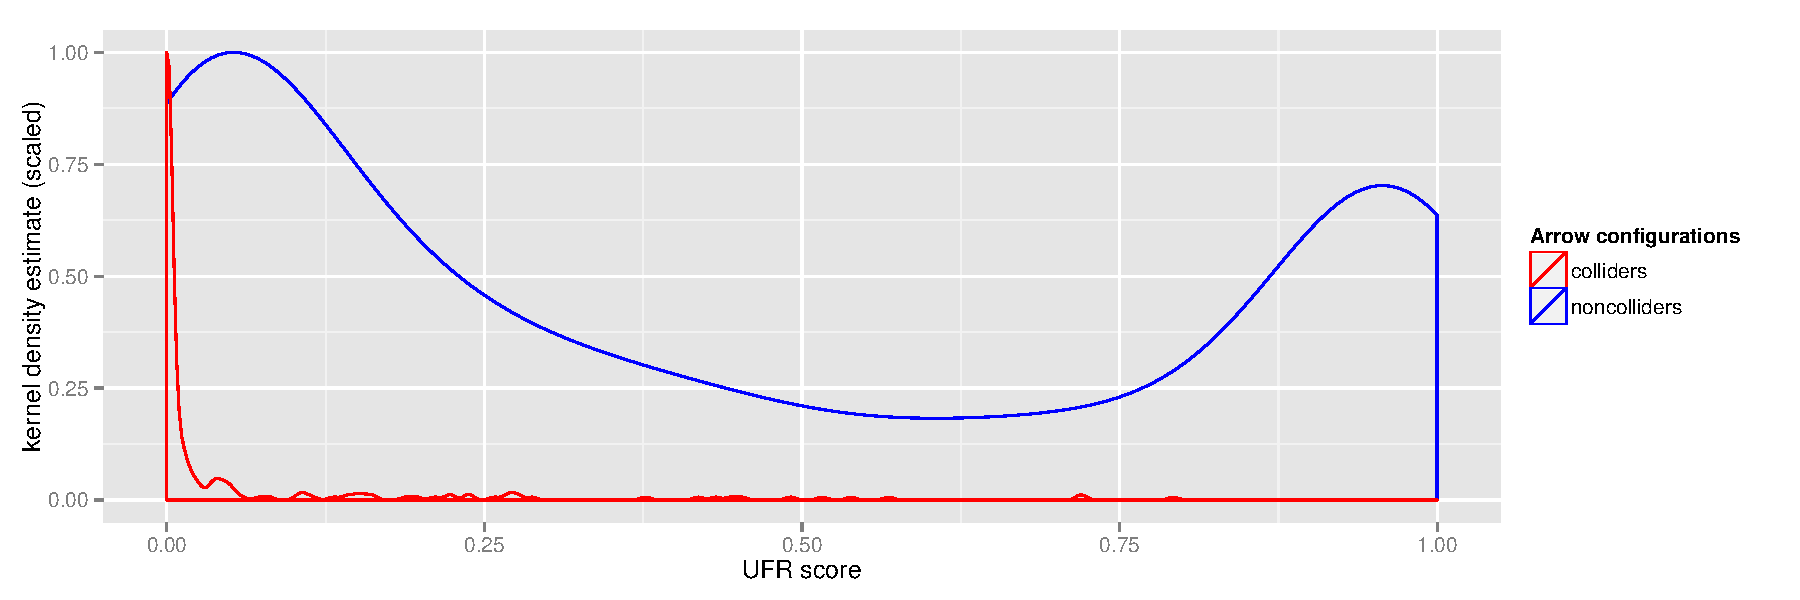
\includegraphics[width=\textwidth]{figures/ufr-density.pdf}
 \caption{UFR scores for collider and non-collider test instances}
 \label{ufr-scores}
\end{figure}

Analysing the precision-recall tradeoff on the $ufr$ values, the optimal threshold in terms of F-score was found to be as low as $0.004$. This is the value I chose to adapt, so that the test $ufr < 0.004$ constitutes the UFR criterion for v-structure detection. 

\subsection{Triangle Score Sum (TSS): aggregating directionality hints}
Another possibility to stabilize directionality inference is to move away from the framework of propagating binary v-structure decisions, instead embracing the fact that on noisy data, the different triples that each link in the skeleton takes part in may yield conflicting evidence of different strength. The obvious idea then is to quantify the directionality evidence present in each triple, and to combine these scores into an aggregate measure where conflicting evidence cancels out, and random spurious patterns in a single triple are overwritten by a larger number of more well-behaved triples. The basic quantification of directionality evidence in a triple can again be expressed in terms of the difference between the three-way overlap we observe, and the overlap we would expect in a non-collider.

If we continue to only consider the unshielded triples that are still present in the skeleton, and try to aggregate an evidence score from these measures, we are frequently faced with the problem that there is an unshielded triple only for one direction, or that there is a severe imbalance in evidence strength for both sides. This means that small errors in the skeleton can still propagate into large errors in directionality inference.

This leads to the idea of not considering only unshielded triples, but all sets of three languages in the dataset for deciding each link, making the directionality inference step independent from skeleton inference. The resulting score infers for every pair of languages in the entire graph whether a connection between them would look directional, based on the triangle scores of that pair with every other language.

In the discussion that follows, shorthands will be used to compactly represent the relevant overlap quantities. For the shared material between each pair of variables, we use the Greek letter corresponding to the member of the triple that is not involved, i.e.\ $\alpha := \frac{c(B,C)}{\min(c(B),c(C))}$, $\beta := \frac{c(A,C)}{\min(c(A),c(C))}$, and $\gamma := \frac{c(A,B)}{\min(c(A),c(B))}$.\\
In addition, I will use $\delta := \frac{c(A,B,C)}{\min(c(A),c(B),c(C))}$ for the amount of information shared between all three variables. In the notation, the hat diacritic will be used to denote expected overlaps, as opposed to observed values. I will be predicting the expected value $\hat{\delta}$ for the overlap based on the other observable overlap ratios, and then derive a quantification of the evidence against the assumed collider from the difference between observed $\delta$ and expected $\hat{\delta}$.

Let us now derive an approximate expression for $\hat{\delta}$ in the pattern $A \arrowLA B \arrowAL C$, which in the absence of latent variables is the only v-structure scenario. The only way in which a cognate set can come to be shared between all three languages in this scenario is if it was already shared between $A$ and $C$, and was borrowed into $B$ from one of the two languages. The percentage of material shared between $A$ and $C$ is given by $\beta$, and the percentage of material in $B$ borrowed from $A$ and $C$ is simply $\gamma$ and $\alpha$, respectively. Assuming independent sampling, the percentage of items which end up in $\delta$ via the transfer $A \arrowLA B$ should be equal to $\gamma \cdot \beta$, and the percentage transmitted via $C \arrowLA B$ should be $\alpha \cdot \beta$. When we simply add up these percentages, we will count some of the expected transferred items twice. The probability for each element in $cog(A,B,C)$ to have been selected twice is simply $\beta$, because this is the 
probability that a random element picked for transfer from $A$ or $C$ is shared by both nodes. We therefore expect $\delta \cdot \beta$ items to have been counted twice. Using this as a correction, we receive $\hat{\delta} = \gamma \beta + \alpha \beta - \hat{\delta}\beta$. Resolving this expression for $\hat{\delta}$, we arrive at the following equation for the expected three-way overlap in a collider:

\begin{equation}
 \hat{\delta}(A \arrowLA B \arrowAL C) := \frac{\beta(\alpha + \gamma)}{1 + \beta}
\end{equation}

Note that we considered the shielded case here. The situation of an unshielded triple is covered by $\beta := 0$, which causes the definition to collapse to $\hat{\delta} = 0$, capturing the intuition I already used in UFR, namely that a v-structure should result in zero three-way overlap that cannot be explained by other paths.

Turning the fitting of $\delta$ to $\hat{\delta}$ into a fit score could be done in a number of ways, but the easiest way turned out to be to form the quotient of the smaller by the larger of the two values, with special treatment for boundary cases to avoid division by zero:

\begin{equation}
   ts(A \arrowLA B \arrowAL C ) :=
   \begin{cases}
     1 - \frac{\min(\delta,\hat{\delta}(A \arrowLA B \arrowAL C))}{\max(\delta,\hat{\delta}(A \arrowLA B \arrowAL C))} & \text{if } \delta > 0 \text{ or } \hat{\delta}(A \arrowLA B \arrowAL C) > 0\\
     0 & \text{if } \delta = 0 \text{ and } \hat{\delta}(A \arrowLA B \arrowAL C) = 0
   \end{cases}
\end{equation}
\linebreak
$ts(A \arrowLA B \arrowAL C)$ measures the strength of evidence which the cognacy overlaps between the three languages provide against the v-structure pattern. Because all triangle scores are on the same scale, but cover overlaps of different strengths, we cannot directly add up these triangle scores to aggregate the directionality information they encode into a global evidence score. To avoid strong influences from languages with little overlap to the pair in question, it is necessary to weight the contributions to the triangle score sum by their relevance to the link in question. One simple way to define these weights is by considering the strength of the connection of the third variable $C$ to either of the two variables involved, and then normalizing these weights to keep the weighted sum in the $[0,1]$ range. In practice, making the weight differences a little more pronounced helped to moderate the contribution of distant third languages, leading me to square the weights before normalization:

\begin{equation}
 w'(A \arrowLA B; C) = \max\left(\frac{c(B,C)}{c(B)},\frac{c(A,C)}{c(A))}\right)^2
\end{equation}

The normalization of weights then happens in the obvious way:
\begin{equation}
 w(A \arrowLA B; C) = \frac{w'(A \arrowLA B; C)}{\sum_{D \notin\{A,B\}} w'(A \arrowLA B; D)}
\end{equation}

Finally, the weighted sum of triangle scores over all third variables $C$ gives us the definition of the \textit{\isi{Triangle Score Sum (TSS)}} after which the directionality inference method is named: 
\begin{equation}
 tss(A \arrowLA B) = \sum_{C \notin\{A,B\}} w(A \arrowLA B; C) \cdot ts(A \arrowLA B \arrowAL C)
\end{equation}

The TSS can be calculated on each link for arrows in both directions, and the results have the same scale, yielding a natural decision criterion in terms of the evidence strength quotient:

\begin{equation}
 sc(A \arrowLA B) = \frac{tss(A \arrowLA B)}{tss(B \arrowLA A)}
\end{equation}

To understand better how TSS works, let us take a look at an example from the Baltic Sea scenario. For the link betwen \ili{Russian} and \ili{Kildin Saami} ($sjd$), the triangles with the heighest weight are given by \ili{Skolt Saami} ($sms$), due to its high overlap with Kildin Saami, as well as by \ili{Polish} ($pol$) and \ili{Belarusian} ($bel$), both due to their high overlap with Russian. Together, these three triangles account for $62.3\%$ of the total weight sum, meaning that if a strong tendency arises from these three triangles, it will not be inverted by the remaining low-overlap triangles. Let us start with $ts(sjd \arrowLA rus \arrowAL bel)$. If this were a true v-structure, we would expect a three-way overlap of 34.55 cognates. In reality the overlap is higher at 47, giving a moderate counterevidence score of $ts(sjd \arrowLA rus \arrowAL bel) = 0.265$. From the reverse perspective, we have a much better fit at $ts(rus \arrowLA sjd \arrowAL bel) = 0.068$, because the prediction in this case 
would be an overlap of 50.42 cognates. The first triangle thus delivers a score contribution that is almost four times higher for the arrow direction $rus \arrowLA sjd$. The scores for the other two triangles we consider point in the same direction: $ts(sjd \arrowLA rus \arrowAL pol) = 0.362$, but $ts(rus \arrowLA sjd \arrowAL pol) = 0.105$, and $ts(sjd \arrowLA rus \arrowAL sms) = 0.232$ is much higher than $ts(rus \arrowLA sjd \arrowAL sms) = 0.073$. From these three triangles, we can begin to approximate $tss(rus \arrowLA sjd) = 0.300 \cdot \frac{0.068}{0.265} + 0.165 \cdot \frac{0.105}{0.362} + 0.148 \cdot \frac{0.073}{0.232} + \dots \approx 0.2786$. The actual value with the full triangle sum is $tss(rus \arrowLA sjd) = 0.6658$, i.e. the missing triangles will equal the score out quite a bit, although the general tendency for more evidence against $sjd \arrowLA rus$ (i.e. a signal against the wrong directionality) remains.

The challenge of the TSS approach is to decide on a threshold for turning the evidence strength quotient $sc(A \rightarrow B)$ on each link into a directionality decision $A \arrowLA B$. For instance, is $sc(A \arrowLA B) = 0.667$, i.e.\ 50\% more evidence in this direction than the other, enough to make the decision? Reusing the five scenarios generated to derive the best $ufr$ threshold, I extracted the 211 links that were not part of the phylogenetic tree, of which 187 are monodirectional. For each link $A \arrowLA B$ I computed $sc(A \arrowLA B)$. If $sc(A \arrowLA B) < 1.0$, evidence pointed in the right direction, making this an instance where TSS worked correctly. Counterbalancing this are the cases where $sc(A \arrowLA B) > 1.0$, i.e. where the implied arrow was inverted. Figure \ref{ufr-scores} shows the distribution of $sc(A \arrowLA B)$ for the good instances, and the inverse for bad instances. The separation is disappointingly bad, indicating that the possible advantage of a pairwise criterion 
like TSS over a triple-based like UFR is much reduced by the more difficult classification task. Still, it is clearly visible that the correct arrows tend to cluster closer to 0, and the inverted arrows closer to 1. This gives me an empirical basis for deciding on a threshold value, because I want as many good instances as possible below the threshold, while keeping as many bad instances as possible above it, because I prefer not assuming an arrow at all to inferring wrong directionality of contact.

\begin{figure}
 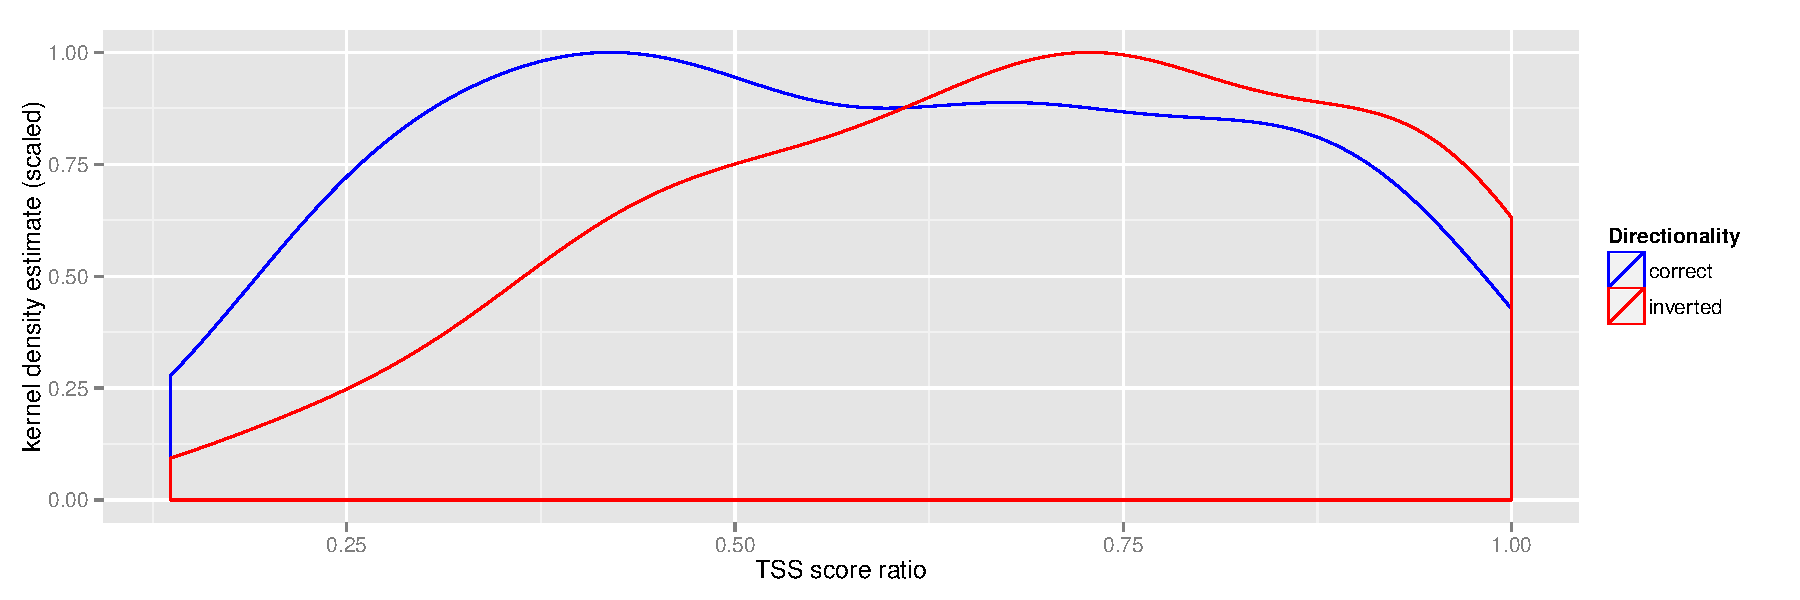
\includegraphics[width=\textwidth]{figures/tss-density.pdf}
 \caption{TSS scores for correct and inverted arrows}
 \label{tss-scores}
\end{figure}

This is another instance of a precision-recall tradeoff, where in addition to the correct and inverted TSS scores, the bidirectional links filter in as additional false instances in either direction. Aiming for a precision of 70\%, we can only get a recall of 21\% with a threshold value of 0.424. On the other hand, if we want to find two thirds of all arrows (66\% recall), we can only achieve that with a threshold of 0.982, i.e. we would have to add arrows very aggressively. A good compromise needs to be found somewhere between these values. Precision remains about constant at 64\%, i.e. about two thirds of inferred arrows are correct, across a very large range of threshold values between 0.555 and 0.720, which is when it starts to drop significantly. At the threshold value of 0.72, the maximum of this range, recall is at 47\%, which seems to be a reasonable compromise given the overall low performance.

In these considerations, we have not considered how the performance of TSS and UFR varies with the number of shared cognates defining each link, i.e. with data sparseness. Unavoidably, the rather simple TSS method can easily be misled by noisy or sparse data. My general impression is that TSS works considerably better on the NorthEuraLex data than the test cases suggest, possibly because the relevant contacts shaping real datasets tend to include large numbers of cognates. The evaluation will shed more light on this question, showing that the intuition is largely, but not always, correct.

\section{The phylogenetic guide tree}
As explained at the start of this chapter, in order to infer fully general evolutionary networks via causal inference, I will need to infer data for the proto-languages. To establish the proto-languages that need to be reconstructed, and as a guiding datastructure for the reconstruction, I need some phylogenetic tree over the attested languages as a starting point. A fully integrated system that starts with word lists and returns a lexical flow network as a result, would therefore include at least a rudimentary component for phylogenetic tree inference. As we have seen in Section 2.5.2, phylogenetic tree inference is already a very well-established field, and any of the methods discussed by \cite{felsenstein2004} can in principle be used for this purpose.

The purpose of my investigation is to compare the performance of different network inference variants on the best possible guide tree, and not to provide a fully integrated software package. My software implementation therefore requires the user to specify cognate sets over the input data, and some phylogenetic tree over the same languages, with branch lengths. This leaves it to the user to plug in cognate detection or tree inference algorithms of their choice, making it possible for my system to profit from future advances in these two subfields, although basic methods for a one-pass processing from word lists to lexical flow network will be provided as part of the release version of my software.

For my experiments on the simulated data from Chapter 5, I will simply use the binary tree created by the simulated language split events, together with the branch lengths defined by the times at which these events occurred. This tree is then reduced to the languages which still lived at the end of the simulation, first removing all the branches leading only to extinct languages, and then removing non-branching nodes in the resulting tree while maintaining consistent branch lengths.

For the NorthEuraLex data, I will use the expert tree defined by Glottolog, again reduced to only those leaves which are attested in the database. Adding branch lengths to this non-binary tree is one of only two places where I found it necessary to use existing phylogenetic inference tools. According to a suggestion by Gerhard Jäger, the inferred cognates were encoded as binary features and given to the IQ-Tree software \citep{nguyen_ea_2015} as input for inferring branch lengths on the unrooted Glottolog tree. For the output, the tree was re-rooted with Mandarin Chinese (\textit{cmn}) as an outlier. None of the family-internal branch lengths inferred by the selected model GTR2+FO+ASC+G4 seemed unplausible on inspection (see Appendix B.2 for a visualization), so that the resulting tree seems adequate as input for reconstruction methods.

\section{Deriving proto-language models}
If I want to be able to treat proto-languages as observed variables in the causal inference paradigm, I need to put some effort into deriving at least a good hypothesis about the presence or absence of each cognate class at each ancestral node in our phylogenetic tree. The idea essential to reconstruction then is to assume that the proto-language of some group of observable languages is most likely to have contained those cognate sets which are present in a large (and diverse) subset of its descendant languages.

This is very similar to the reconstruction of ancestral genomes in bioinformatics, from where we can take a variety of readily applicable algorithms. In addition to the mainstream ASR (Ancestral State Reconstruction) techniques in this tradition, I also present a naive threshold-based approach that will be used as a baseline. After evaluating the different methods on the simulated data, only the best two methods will be used to arrive at a usable reconstruction of ancestral cognacy in the NorthEuraLex dataset, and this reconstruction will be treated just like actual observations for phylogenetic network inference.

\subsection{Ancestral state reconstruction algorithms}
From the large number of ASR methods discussed in the literature, I will only sample a few very common and robust variants that are trivial to extend from nucleotides to cognacy data. The treatment of the methods cannot be complete, and I neither have the space to give examples of each reconstruction algorithm here, nor to provide the full algorithmic details for each method. Still, my explanations should suffice to provide the reader with correct intuitions about each method, and the formal statements are precise enough to completely describe the core features of any implementation.

\subsubsection{Naive threshold-based approaches}
For the initial experiment, I opted for a simple recursive criterion. For each node in the expert tree, it includes those cognate sets that are present in a majority (more than 50\%) of its immediate daughter languages. This implies we start at the observable languages and their cognate sets, and reconstruct upwards in the expert tree, arriving at the root language(s) in a single bottom-up pass through the entire tree.

If we introduce the notation $P(l = A)$ for the probability of cognate class $A$ being reconstructed for some concept in the language $l$ with children $l_1,\dots,l_k$, the \isi{majority-based reconstruction} can be written as a recursive formula
\begin{equation}
   P(l = A) :=
   \begin{cases}
     1 & \text{if } \frac{1}{k} \sum_{i=1}^k P(l_i = A) > 0.5\\
     1 & \text{if } k = 0 \text{ and the word for the concept was assigned to class } A\\
     0 & \text{else }
   \end{cases}
\end{equation}
\linebreak
This simple definition directly implements an important property of any useful reconstruction, namely that a word which was borrowed once at an intermediate stage and therefore now turns up in every language of a branch with many languages, will not end up in the proto-language if there is no other branch which also features a cognate. This usage of the tree to channel the information is superior to an even more naive criterion that would simply count the occurrences of each cognate class at the leaves under each ancestral node.

The main problem of this approach is of course that it tends to err very much on the safe side, as reconstruction stops as soon as there is a configuration of two subgroups for which different ancestral states are reconstructed, which occurs very often in real data. On the other hand, the few reconstructions this method arrives at tend to be extremely reliable. A threshold lower than 0.5 could be introduced for nodes which are more than binary-branching, but this would quickly lead to far too generous reconstruction.

In sum, threshold-based approaches can only be expected to show a very low performance, and do not offer many options to fine-tune them to the specific task. I will still use the majority-based approach as a baseline for comparison with more advanced alternatives.

\subsubsection{Parsimony-based approaches}
The most direct modern approach to ASR is based on maximizing parsimony, which can be seen as a formalization of Occam's razor, i.e.\ the principle of selecting the simplest hypothesis which explains all the data. In the context of ASR, parsimony can simply be described by the number of state changes which the model needs to assume. If we reconstruct the ancestral states in such a way that the number of mutations the model needs to assume is minimized, we are maximizing the parsimony of our reconstruction.

The standard algorithm for maximum parsimony is the \isi{Sankoff algorithm}, originally defined by \cite{sankoff1972}, which uses dynamic programming to keep track of the minimal number of replacement operations which needs to be assumed for smaller subproblems, and fills a table for each node, storing the total number of replacement operations which each state at that node would imply. For the current optimal solution in each cell, backpointers are stored which make it possible to reconstruct the configuration of ancestral states which led to the minimum number of replacement events for the entire problem. In my application, there are two useful variants of this basic Sankoff algorithm, which differ in whether we consider the presence of each cognate set as an independent character, or treat the different cognate sets for one concept as the different values of a single multistate character.

In the first version, which I will call \textit{\isi{multi-value MP reconstruction}}, a separate run of this basic Sankoff algorithm is performed for each presence-absence character, meaning that the table for each node only has two cells (one for presence, one for absence). Formally, each cognate set $A$ is reconstructed for the subset $L_A \subseteq L$ of all languages for which $\sum_{(l_i,l_j) \in E} 1_{l_i \in L_A, l_j \notin L_A}$ is minimal, under the condition that $l \in L_A$ holds for every language $l$ where the cognate set $A$ is attested, and $l \notin L_A$ for every language $l$ where it is not. In this version, it is possible that absence is reconstructed for all cognate sets, leaving a node without reconstruction, or that presence is reconstructed for more than one cognate set at a given node, hence the name I am using.

The second version, which I will call \textit{\isi{single-value MP reconstruction}}, reconstructs exactly one cognate set from the set of ancestral nodes, out of a set of candidates defined by the cognate sets occurring in the attested languages assigned to that phylogenetic unit. The Sankoff table has as many cells as there are candidate cognate sets. Formally, given a cost function $c(A,B)$ for the replacement of cognate sets (typically, $c(A,A) := 0$ and $c(A,B) := 1$ for $A \neq B$), this variant assigns a tuple of cognate sets $(A_1,\dots,A_n)$ to all the nodes $(l_1,\dots,l_n)$ such that that $\sum_{(l_i,l_j) \in E} c(A_i,A_j)$ is minimal, while keeping one set $A_j$ of the cognate sets  assigned to each attested language $l_j$ fixed.

The main problem of parsimony-based ASR is that different branch lengths cannot be accounted for. This exploits existing knowledge only suboptimally, since if one of two languages forming some phylogenetic unit is known to be more conservative (which would be reflected by a shorter branch length or a lower replacement rate in phylogenetic tree models), this will make it more likely that the ancestral set survived in this language, making it more informative for the reconstruction. A related more general problem of MP is that there will often be a large number of maximally parsimonious reconstructions, i.e.\ parsimony alone does not give us a sufficient decision criterion for finding a single reconstruction.

\subsubsection{Fully probabilistic approaches}
More recent approaches to ASR work in the maximum-likelihood (ML) paradigm. These fully probabilistic methods treat the discrete states $y$ at internal nodes as unknown parameters whose values need to be estimated given the data $x$ we observe. An obvious choice is the maximum likelihood estimator, which maximizes $P(y|x)$, the probability of different parameter values given the observed data, with the help of Bayes' rule:
\begin{equation}
 P(y|x) = \frac{P(x|y)P(y)}{\sum_y P(y)P(x|y)}
\end{equation}
While the denominator is hard to compute, it is independent of $y$ and is therefore irrelevant for maximizing the expression. Maximum likelihood estimation assumes that no prior information about plausible values $P(y)$ is available, which reduces the task of maximizing $P(y|x)$ to maximizing the likelihood $P(x|y)$ that we see the data given parameter values $y$. A good ML estimator will typically converge to the most likely value of $y$, although it is possible that other values of $y$ are almost as likely, and that the ML estimate $\hat{y}$ is even an outlier in the space of plausible parameter values. Still, ML estimates of model parameters provably maximize the agreement of the model with the data in many types of inference problems, given ML estimation a strong independent motivation outside the Bayesian paradigm.

In the application to ASR, optimization is based on an explicit parameterized evolutionary model $P_{ij}(\theta)$ which fully describes how each state $i$ is likely to evolve along a given phylogenetic tree, and thereby assigns a probability $P(x|y,\theta)$ to the observed data for each set of parameter values. If the evolutionary model is Markovian (the probability of each state change only depends on the parent state, not on earlier states), dynamic programming can be used to efficiently derive the internal states $y$ which maximize $P(x|y,\theta)$. For different applications, different evolutionary models are plugged into this basic paradigm.

Apart from the different evolutionary models, the main dividing line between approaches to ML-based ASR is in the method the optimal ancestral states at internal nodes are calculated. In the computationally simpler \isi{marginal reconstruction} as introduced by \cite{yang_ea_1995}, reconstruction of states at an internal node $A$ is done by re-rooting the tree such that $A$ becomes the root, and then computing the likelihoods for the different states at each node in a bottom-up fashion, summing over all possible combinations of states in the children $ch(A) = \{B_1,\dots,B_n\}$ down to the leaf nodes:
\begin{equation}
 \hat{y}_A :=  \arg \max_i L_A(i),\ L_A(i) := \sum_{j_1,\dots,j_n} \prod_{k=1}^n P_{ij_k}L_{B_k}(j_k)
\end{equation}
These values can again be computed by dynamic programming, meaning that the computation is only more time-consuming than the Sankoff algorithm by a factor linear in the number of ancestral nodes.

By contrast, in the more complex \isi{joint reconstruction}, the likelihood is jointly maximized over reconstructed values at all nodes, which is computationally a lot more demanding. Moreover, according to \cite{yang_ea_1995}, this variant is less suitable for retrieving optimal reconstructions at each ancestral node (because suboptimal local solutions can be necessary for an optimal global reconstruction), which leads me to disregard it as an option for the current application.

Implementing marginal reconstruction from stretch is non-trivial, and the implementation details of existing systems are not fully specified in the literature. This makes ML reconstruction the second of the two places in my infrastructure where it seemed more prudent to rely on third-party software instead of engineering my own implementation to behave exactly like a reference implementation. For marginal ML reconstruction, I am using a somewhat brittle interface from my Java code into the R package \texttt{phangorn} via system calls to \texttt{Rscript}, and a custom method on the R side for output in a Nexus format which can be read back into Java and mapped onto the original character information.

In analogy to multi-value MP reconstruction, \textit{\isi{multi-value ML reconstruction}} operates on binary characters which encode the presence or absence of each cognate set at each node. For non-attested nodes, the marginal reconstruction assigns probability values to each of the two values \texttt{0} (absence) and \texttt{1} (presence) of each character. If the probability of \texttt{1} at an ancestral node is above 50\%, the corresponding cognate set is reconstructed for the respective proto-language. This variant shares its basic properties with multi-value MP reconstruction. Ancestral nodes can remain without any reconstructed cognate set if for each cognate set character, the probability of the value \texttt{1} was below 50\%.

For \textit{\isi{single-value ML reconstruction}}, we only use one multi-state character for each concept, where each state encodes one of the possible cognate sets. The marginal reconstruction then produces a probability distribution over all the possible cognate sets at each ancestral node, and we only reconstruct the one with the highest probability. The behavior of the resulting method is again similar to single-value MP reconstruction in that exactly one cognate set will be reconstructed for each ancestral node. Due to limits in the \texttt{phangorn} implementation which are well-justified for its main field of application in biology, there is no support for ambiguity in the input data. This prevented me from modeling the synonyms in the NorthEuraLex data, so that the single-value ML reconstruction only builds on the first form in each list of concept realizations.

Maximum-likelihood methods for ASR work on a single phylogenetic tree with branch lengths, which is typically inferred by a different (often Bayesian) method. This can lead to problems because the likelihood of the individual tree hypothesis that the reconstruction is based on is usually quite low, and a reconstruction which takes more than a point estimate of plausible trees into account will be much more sound if computationally feasible.

To account for the uncertainty in the tree reconstruction, Bayesian methods which account for the uncertainty in both the ancestral characters and the tree structure have been developed. The hierarchical Bayes method by \cite{huelsenbeck_bollback_2001} is able to model uncertainty in the tree, branch lenghts, and the substitution model at the same time, but is reported to lead to very high uncertainty in the results. The advantages of this more accurate quantification of uncertainty are unclear in an application where only a single optimal reconstruction can be used. This and the prohibitive computational complexity associated with fully Bayesian methods justify confining myself to the simpler maximum-likelihood paradigm.

\subsection{Evaluation of ASR algorithms on simulated data}
It is easy to evaluate the different ASR methods on the simulated data. Let us act as if we lost the true configurations of all dead languages in the simulated set, and are left with a reduced version of the true tree which only contains the living leaves, plus the internal nodes which are necessary to keep the branching structure over these leaves. We can then feed the reduced true tree and the data from the leaves into the different reconstruction algorithms.

To compare the results, we return to the true data we discarded, and compute the percentage of bits (representing presence or absence of each cognate class) at the reconstructed nodes that correspond to the true values, as well as precision and recall on the level of reconstructed classes. Finally, we analyse the difference in reconstruction quality for proto-languages of different age, to find out whether one of the algorithms is more robust at higher time depths.

The following five previously introduced ASR methods were compared in this way:
\begin{enumerate}
  \item \textbf{Mjrty} (majority-based), i.e.\ using the naive criterion of reconstruction or presence in the majority of children
  \item \textbf{MPsgl} (single-value MP), i.e.\ using the Sankoff algorithm to reconstruct exactly one correlate set for each concept at each node
  \item \textbf{MPmlt} (multi-value MP), i.e.\ using the Sankoff algorithm to reconstruct a binary presence/absence value for each correlate set and concept
  \item \textbf{MLsgl} (single-value ML), i.e.\ using a marginal estimator on multistate characters, and selecting the most likely cognate set for each ancestral node
  \item \textbf{MLmlt} (multi-value ML), i.e.\ using a marginal estimator on binary presence/absence values, reconstructing the correlate set if presence is more likely than absence
\end{enumerate}

Running the different reconstruction algorithms and comparing the results on our 50 simulated linguistic histories, we get the numbers in Table \ref{asr-overall-results}. The overall picture is clearly in favor of the MP and ML methods, but the differences between the two are not very pronounced. Only for the single-value variants, there is a clear advantage for ML over MP. For both MP and ML, the single-value variants shows higher recall than the multi-value variants, because they always produce some reconstruction even if evidence is not very strong, but this comes at a significant cost to precision. The very conservative majority method has the highest precision, but achieves this at a much higher cost to recall than the MLmlt method almost equalling it in precision. Overall, MLsgl is clearly the best method, as it achieves the highest recall by a significant margin, without compromising too much on precision.

\begin{table}
 \centering
 \begin{tabular}{cccccc}
  \hline \hline
  \# & Mjrty & MPsgl & MPmlt & MLsgl & MLmlt\\ \hline
  Accuracy & 0.9804 & 0.9774 & \textbf{0.9830} & 0.9803 & 0.9829\\
  Precision & \textbf{0.8463} & 0.5720 & 0.8199 & 0.6292 & 0.8255\\
  Recall & 0.3212 & 0.5874 & 0.4586 & \textbf{0.6289} & 0.4386\\
  F-score & 0.4656 & 0.5796 & 0.5882 & \textbf{0.6291} & 0.5813\\
  \hline
 \end{tabular}
 \caption{Performance of different ASR algorithms on simulated data}
 \label{asr-overall-results}
\end{table}

To check the suspicion that the differences between the algorithms might become more pronounced at higher time depths, where the few really difficult reconstructions are, we can evaluate the performance separately on proto-languages of different ages. Figure \ref{asr-results-by-age} visualizes the performance of the five reconstruction methods across twenty different age ranges.

\begin{figure}
 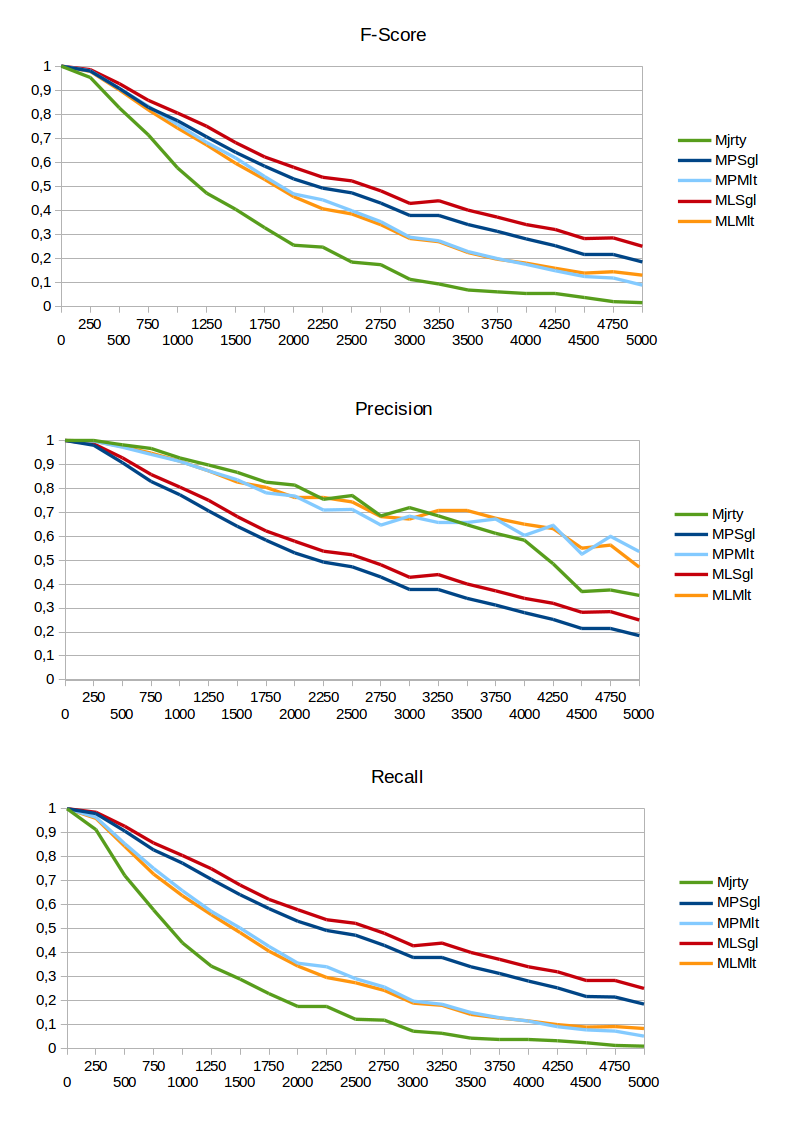
\includegraphics[width=\textwidth]{figures/recon-eval-timedepth.png}
 \caption{Development of ASR performance with age of reconstructed language}
 \label{asr-results-by-age}
\end{figure}

Whereas F-scores are satisfactory for reconstructed languages that go back only a few hundred simulated years, already at a time depth of 1,000 years substantial differences in the performance of the different algorithms start to appear. At higher time depths, recall becomes so low that the F-scores are already surprisingly close to zero. Still, there are some interesting developments at this highly problematic range. At a time depth of 5,000 years there is a clear split between three methods which essentially do not reconstruct anything useful any more (the majority method and the multi-state methods, all with recall under 10\%), and the other three methods which still manage to reconstruct at least some cognate sets (recall of 20-30\%), albeit with a high error rate (less than 40\% of the reconstructed cognate sets are correct). We can conclude that the acceptable overall performance of all methods in the previous analysis was mainly due to the dominance of simple reconstruction tasks if we evaluate across 
entire trees with many more younger languages than old ones. The task of reconstruction at higher time depths is still very much an unsolved problems. At these higher time depths, the two multi-state methods perform better precisely because they are biased towards assuming some reconstruction even if not enough evidence is available. However, since the overall advantage of the maximum-likelihood methods remains stable for proto-languages of any age, we at least know that they are clearly our best methods for phylogenetic flow inference, and will therefore be the default reconstructions used for the further experiments. The superiority of ML reconstruction over MP reconstruction was recently confirmed by \cite{jaeger_list_2017} on a different test set comprising real data from Indo-European, Austronesian, and Sinitic languages. In contrast to my simulated data, the performance of the methods is only evaluated against reconstructions at the level of the respective proto-language, i.e. at a high time depth. Just 
as in my experiment, the ML-single variant (ML-multi in their terminology) wins by a large margin.

\section{Phylogenetic Lexical Flow Inference (PLFI)}
Given a tree skeleton predetermined either by previous knowledge or inferred by means of a phylogenetic method, we can now apply ASR methods to derive cognate sets for the tree's internal nodes, and proceed to apply causal inference to the resulting dataset. Of course, this means that the performance of the method will hinge very much upon the quality of the reconstruction.

Very optimistically assuming that the output of our ASR method approximates the true history very closely, we treat all the nodes in our phylogenetic tree as observable languages, and apply lexical flow inference to a mixture of attested languages and reconstructed proto-languages. This is the algorithm which I propose to call \isi{Phylogenetic Lexical Flow Inference (PLFI)}. Algorithm \ref{plfi-algorithm} gives a description of all PLFI variants in pseudocode.

The PLFI algorithm requires either an expert tree, or a tree inferred by some phylogenetic tree inference algorithm, as input in addition to the cognacy data. After a preprocessing stage where the tree is reduced to the leaves for which data are available, some ancestral state reconstruction method (MLsgl by default) is applied to the tree and the data at the leaves in order to infer the presence or absence of each cognacy class at every non-leaf node in the reduced tree. The causal graph is then built over all the tree nodes.

The PC algorithm starts out with the fully connected graph, i.e. a network in which every pair of nodes is connected by a link. This graph is progressively thinned out to yield the skeleton by means of conditional independence tests based on separating set candidates. In each iteration, the algorithm increases the size $s$ of separating sets it considers. At each stage, it iterates through all the links remaining in the graph, and tries to build a separating set of size $s$ from the neighbors of the two languages it tries to separate.

Unlike in the vanilla PC algorithm, there is a defined order in which the links are tested for deletability. The PLFI algorithm always starts with the weakest remaining link, on the grounds that such links are more likely to arise due to random fluctuation in the noisy cognacy judgments. The links which represent the highest overlap are always checked last.

The separating set candidates which are tried out for the conditional independence tests depend on the skeleton inference method. If the skeleton inference method is set to $FS$, the flow-separation criterion introduced in Section 6.4 is applied, so that every separating set candidate is composed of paths connecting the two languages in the current skeleton. Using one of the other skeleton inference methods, this first stage of the algorithm can also be configured to behave just like the vanilla PC algorithm or like PC*.

For the directionality inference stage, the user has the choice between four variants. The vanilla PC variant only differs from stable PC and the UFR criterion in the way in which v-structures are detected. In all three cases, the three standard directionality propagation rules of the PC algorithm are applied until all links are directed or none of the rules applies any longer. The only directionality inference method which works differently is the TSS-based variant, which infers the directionality on each arc separately by checking the TSS ratio against the threshold determined in Section 6.5. 

\begin{algorithm}\footnotesize
  \begin{algorithmic}[1]
  \STATE ASR method $asrM \in \{Mjrty,MPsgl,MPmlt,MLsgl,MLmlt\}$
  \STATE skeleton inference method $sklM \in \{PC,PS,FS\}$
  \STATE directionality inference method $dirM \in \{VPC,SPC,UFR,TSS\}\)
  \STATE $T := phyloInference(\{L_1,\dots,L_n\})$, or an expert tree
  \STATE $T := reduce(T,\{L_1,\dots,L_n\})$, the phylogenetic tree reduced to attested leaves
  \STATE $T := asr(T,asrM)$, add cognate classes to ancestral nodes by reconstruction
  \STATE $\mathcal{L} := nodes(T)$
  \STATE $G := (\mathcal{L},E) := (\mathcal{L},\{\{L_i,L_j\}\ |\ L_i, L_j \in \mathcal{L'}\})$, the complete graph
  \STATE $S \colon \mathcal{L} \times \mathcal{L} \rightarrow \wp(\mathcal{L})$, the separating set storage
  \STATE $s := 0$
  \WHILE{$s < |\mathcal{L}| - 2$}
    \FOR{$\{L_i,L_j\} \in G$ by increasing strength of remaining flow}
      \IF {$sklM \in \{PC, PS\}$}
        \FOR{each subset $S \in \wp(N)$ for neighbors $N$ of $L_i$ or $L_j$}
          \IF {$sklM = PC$ or all elements of $N$ are on paths from $L_i$ to $L_j$}
	        \IF {$|S| = s$ and $I(L_i;L_j|S) < 0.025$}
	          \STATE remove $\{L_i,L_j\}$ from $G$, $S(L_i,L_j) := S(L_i,L_j) \cup \{S\}$
	        \ENDIF
          \ENDIF
	    \ENDFOR
      \ELSIF {$sklM = FS$}
	    \FOR{each combination $P_1,...,P_k$ of paths from $L_i$ to $L_j$ of length $\leq 4$}
	      \IF {$|S| = s$ for $S := \bigcup\{P_1,\dots,P_k\}$}
	        \IF {ratio of $c(L_i,L_j)$ not explainable by flow across $S$ is $<$ 0.025}
		      \STATE remove $\{L_i,L_j\}$ from $G$, $S(L_i,L_j) := S(L_i,L_j) \cup \{S\}$
	        \ENDIF
	      \ENDIF
	    \ENDFOR
      \ENDIF
    \ENDFOR
    \STATE $s := s + 1$
  \ENDWHILE
  \IF {$dirM = TSS$}
    \FOR{$\{L_i,L_j\} \in G$}
      \IF{$sc(L_i \arrowLA L_j) < 0.72$}
         \STATE add arrow $L_i \rightarrow L_j$ to network
      \ENDIF
    \ENDFOR
  \ELSE
    \FOR{$L_i,L_j,L_k \in \mathcal{L}$ where $\{L_i,L_j\},\{L_j,L_k\} \in E$ but $\{L_i,L_k\} \notin E$}
      \IF{$(L_i \rightarrow L_j \leftarrow L_k)$ is a v-structure according to $dirM$ and $S(L_i,L_k)$}
	\STATE add arrows $L_i \rightarrow L_j$ and $L_k \rightarrow L_j$ to network
      \ENDIF
    \ENDFOR
    \STATE propagate arrows according to rules $\mathcal{R}_1$ to $\mathcal{R}_3$
  \ENDIF
  \RETURN network consisting of $G$ and arrows
  \end{algorithmic}
  \caption{PLFI($L_1,\dots,L_n$)}
  \label{plfi-algorithm}
\end{algorithm}

\section{Evaluation of PLFI}
There are two main ways to evaluate phylogenetic lexical flow inference which promise to be of interest. First, we can evaluate on perfect proto-data to determine the theoretical maximum performance the method could achieve if we had access to a perfect reconstruction. This gives us an upper bound on performance, because any real reconstruction will deviate from this perfect picture. To generate the input data for PLFI, we simply take the final state of the simulation for all languages, whether living or dead. This implies we include data from entire unattested lineages, including what we have earlier called para-languages and substrates, so that in this scenario, we have actual causal sufficiency, and the PC algorithm should be applicable without restrictions.

The more realistic evaluation of the method builds on reconstructed proto-data. Here, we reduce the known tree to ancestors of living languages, leaving only the lowest common ancestor in the cases were internal nodes become unary because one of two branches is deleted. Then, we apply one of the ASR algorithms to produce the data for the internal nodes of the reduced tree. To limit the number of cases to consider, we only evaluate on the two ML reconstruction methods which performed best on the simulated data, in order to be certain that our findings on simulated data carry over to the NorthEuraLex dataset.

\subsection{Evaluation metrics for phylogenetic flow}
Since causal inference as we employ it consists of the two stages of skeleton inference and directionality detection, for both of which we have multiple options at our disposal, it makes sense to first evaluate performance at the skeleton inference task, and then evaluate the different methods for directionality detection on the results of the best skeleton inference method.

For each connection $L_1 \arrowLL L_2$ which was found by the phylogenetic flow algorithm in the reconstructed network $G_{res}$, we can ask whether it corresponds to a lateral connection $L_1 \arrowLL L_2$ in $G_{true}$. If this is the case, we call the inferred connection a true positive ($tp$), otherwise a false positive ($fp$). If a lateral connection in $G_{true}$ does not have an equivalent in $G$, we count it as a false negative ($fn$). If for a pair of languages $L_1$ and $L_2$, neither graph has a connection $L_1 \arrowLL L_2$, we count it as a true negative ($tn$). From these four numbers $tp$, $fp$, $fn$, and $tn$, we can compute precision and recall, the standard measures of performance on binary classification tasks. The \textit{\isi{skeleton recall}} (SkRc) is then defined as $\frac{tp}{tp+fn}$, i.e the ratio of links in the true skeleton which the algorithm managed to reconstruct. Analogously, the \textit{\isi{skeleton precision}} (SkPr) can be written as $\frac{tp}{tp+fp}$, i.e.\ the ratio of 
links in the reconstructed skeleton which are correct. Both measures can be combined in a standard way via $2 \cdot \frac{SkPr \cdot SkRc}{SkPr+SkRc}$ to the \textit{\isi{skeleton F-score}} (SkFs), a combined performance measure which reaches high values if precision and recall are well-balanced.

For the evaluation on perfect proto-data, it is easy to adapt these standard performance measures, because there are no complications due to gaps in our knowledge which ASR cannot close. When evaluating on reconstructed proto-data, the situation is a little more complicated because some of the true connections cannot conceivably be found in the absence of substrates, and even in a perfect result, only the links between ancestors of related languages will be represented. For simulated contacts between pairs of languages where either only the donor or recipient of lexical material is in the input data (again, cases like substrate languages), we need to define which structures in the result graph would count as correctly reflecting reality, and which structures we would not accept as equivalent to the true story. In terms of precision, we will accept a link where either the reconstructed donor or the reconstructed recipient is the lowest ancestor of the true donor or recipient in the reduced tree, but not if 
both donor and recipient are wrongly detected, or contact is inferred between descendants. For each connection $L_1 \arrowLL L_2$ in the inferred network $G_{res}$, we therefore ask whether it is compatible with some connection in $G_{true}$, in the sense that it reflects a lateral connection $A_1 \arrowLL A_2$ for two languages $A_1 \in anc(L_1)$ and $A_2 \in anc(L_2)$ in $G_{true}$. For example, if a link $isl \arrowLA eng$ is found, we would accept it on the grounds of $North\ Germanic \arrowLA eng$.

While the definition of true positives and false positives remain rather straightforward in this way, the definition of false negatives becomes a bit more involved. Is $North Germanic \arrowLA eng$ captured by the inferred skeleton if it features a connection from any North Germanic\il{North Germanic languages} language to \ili{English}? Or should we require that all North Germanic languages should be connected to English by a lateral connection? Recall that the last option would require separate exclusive lexical flows of detectable size from every single North Germanic languages into English, which will typically not be possible. For this reason, I choose to relax the condition and only require the weaker representation. More formally, a link $L_1 \arrowLL L_2$ in $G_{true}$ which is not present in $G_{res}$ does not count as a false negative if there are descendants $D_1 \in des(L_1)$ and $D_2 \in des(L_2)$ in the phylogenetic tree such that $D_1 \arrowLL D_2$ in $G_{res}$.

With the skeleton in place, we can proceed to measure the quality of directionality inference on the links. The idea is to consider all correct links in the skeleton for which a directionality can be derived from the gold standard, and then analyse for which of these links the correct orientation was inferred. The fact that we actually have three possibilities for the gold standard ($\arrowLA$, $\arrowOA$, and $\arrowAA$), relative to which we have three possibilities for the result ($\arrowLA$, $\arrowAL$, $\arrowLL$), makes it a little less natural to define positives and negatives than for the skeleton measures. However, if we decide to count an arrow which points in the wrong direction as a false positive, and take the equivalence of $\arrowLL$ and $\arrowAA$ as well as the compatibility of $\arrowOA$ in the gold standard with both $\arrowLA$ and $\arrowLL$ in the result into account, we arrive at a plausible solution, which is defined by Table \ref{arrow-eval-def}.

\begin{table}
\centering
\begin{tabular}{rlll}
  \hline \hline
  & $\arrowLA$ in result & $\arrowAL$ in result & $\arrowLL$ in result \\ \hline
  $\arrowLA$ in standard & \textit{true positive} + & \textit{false positive} + & \textit{false negative}\\ 
                                  & \textit{true negative} & \textit{false negative} & \\ \hline
  $\arrowOA$ in standard & \textit{true positive} & \textit{false positive} & \textit{true negative}\\ \hline
  $\arrowAA$ in standard & \textit{false negative} & \textit{false negative} & \textit{true negative}\\ \hline
\end{tabular}
 \caption{Table of elementary definitions for arrow evaluation}
 \label{arrow-eval-def}
\end{table}

Based on these elementary definitions, we can again define precision and recall measures in the standard way. Informally, the \textit{\isi{arrow recall}} (ArRc) then measures how many of the arrows in the gold standard on links in the derived skeleton also occur in the inferred network with the correct directionality. To complement this measure, \textit{\isi{arrow precision}} (ArPr) quantifies how many of the arrows in the reconstruction are justified by the gold standard. The trade-off between these two measures is of the same nature which one would typically capture in the precision-recall paradigm. If a directionality inference algorithm aggressively infers arrows even in the face of conflicting or weak evidence, this will increase arrow recall at the expense of arrow precision. A very cautious directionality inference scheme which assumes bidirectionality by default, will lead to a higher arrow precision at the cost of arrow recall. To handle this trade-off, we again mix both measures into the \textit{\isi{arrow F-score}} (ArFs) defined as $2 \cdot \frac{ArPr \cdot ArRc}{ArPr+ArRc}$, which will be our primary measure for comparing the performance of the different variants.

\subsection{Overall quantitative results for NorthEuraLex data}
Our first step for the evaluation is to compare the different methods in terms of skeleton precision and recall as well as arrow precision and recall on the entire NorthEuraLex dataset. This will allow us to choose the best method for the case studies in the next section.

Table \ref{skeleton-evaluation-nelex} compares the skeleton precision and recall obtainable by the different conditional independence checks on our two maximum-likelihood reconstructions. While the single-value ML reconstruction led to the highest overall F-scores in the reconstruction experiments on simulated data, we find that the multi-value reconstruction consistently leads to better performance in all measures, especially in recall. These are the consequences of using the reconstruction with the highest precision, as this reconstruction will introduce the least noise, letting the patterns appear more clearly. The noise introduced by single-value reconstruction is so strong that it not only decreases the precision (leading to spurious lateral connections), but also the recall (letting weaker conditions disappear into the noise).

\begin{table}
 \centering
 \begin{tabular}{ccccccc}
  \hline \hline
   & \multicolumn{3}{l}{MLsgl reconstruction} & \multicolumn{3}{l}{MLmlt reconstruction}\\ 
   & PC & PS & FS & PC & PS & FS\\ \hline
  skPrc & \textbf{0.970} & 0.907 & 0.856 & 0.965 & 0.914 & 0.859\\
  skRec & 0.265 & 0.376 & 0.431 & 0.404 & 0.502 & \textbf{0.557}\\
  skFsc & 0.416 & 0.532 & 0.574 & 0.570 & 0.648 & \textbf{0.676}\\
  \hline
 \end{tabular}
 \caption{Comparing skeleton performance of MLsgl and MLmlt reconstructions on the NorthEuraLex data}
 \label{skeleton-evaluation-nelex}
\end{table}

The arrow performance measures are only defined for the intersection of links in the inferred skeleton and the gold standard, which will be a smaller or a larger set depending on the skeleton performance. Therefore, arrow performance cannot be reliably compared across reconstructions and skeleton inference variants. Still, we can compare the performance of the four directionality inference methods on the best skeleton. This is done in Table \ref{arrow-evaluation-nelex}. As the results show, the two standard directionality inference methods used in the causal inference literature do not work at all, due to the non-exact conditional independence tests and the resulting difficulty to detect v-structures based on separating sets. On the multi-value reconstruction, the stable PC variant does not even manage to infer a single correct arrow. The two directionality inference methods introduced in this chapter fare a lot better, but there is an interesting contrast in their behavior on the different reconstructions. 
The single-value reconstruction gives an advantage to UFR, whereas TSS is clearly superior on the multi-value reconstruction.

\begin{table}
 \centering
 \begin{tabular}{ccccc}
  \hline \hline
   & \multicolumn{4}{l}{FS on MLsgl reconstruction}\\ 
   & VPC & SPC & UFR & TSS\\ \hline
  arPrc & 0.185 & 0.154 & \textbf{0.615} & 0.546\\
  arRec & 0.114 & 0.050 & \textbf{0.585} & 0.585\\
  arFsc & 0.141 & 0.076 & \textbf{0.600} & 0.565\\
  \hline
 \end{tabular}\\[0.5cm]
  \begin{tabular}{ccccc}
  \hline \hline
   & \multicolumn{4}{l}{FS on MLmlt reconstruction}\\ 
   & VPC & SPC & UFR & TSS\\ \hline
  arPrc & 0.240 & 0.000 & 0.410 & \textbf{0.500}\\
  arRec & 0.122 & 0.000 & 0.695 & \textbf{0.689}\\
  arFsc & 0.162 & (0.0) & 0.516 & \textbf{0.579}\\
  \hline
 \end{tabular}
 \caption{Comparing arrow performance of MLsgl and MLmlt reconstructions on the NorthEuraLex data}
 \label{arrow-evaluation-nelex}
\end{table}

Finally, to rank the different variants for overall performance, we can multiply the skeleton and arrow F-scores, capturing the intuition that the best approach should result in both a good skeleton and correct directionality information. The resulting numbers are given in Table \ref{variant-comparison-nelex}, motivating our use of the MLmlt-FS-UFR variant for the case studies. Depending on the application, a different variant which is tuned towards more reliability at the expense of only finding the most prominent patterns, might be preferable. For applications where the focus is on precision (e.g.\ if computational means for deciding a research question are needed), the numbers on NorthEuraLex suggest that the MLsgl-FS-TSS variant might be the best option.

\begin{table}
 \centering
 \begin{tabular}{lccc}
 \hline \hline
PLFI Variant & skFsc & arFsc & skFsc $\ast$ arFsc\\ \hline
\texttt{MLmlt-FS-UFR} & 0.6759 & 0.5793 & 0.3916\\
\texttt{MLmlt-PS-UFR} & 0.6477 & 0.5405 & 0.3501\\
\texttt{MLmlt-FS-TSS} & 0.6759 & 0.5157 & 0.3486\\
\texttt{MLsgl-FS-TSS} & 0.5736 & 0.6000 & 0.3442\\
\texttt{MLsgl-FS-UFR} & 0.5736 & 0.5647 & 0.3239\\
\texttt{MLmlt-PS-TSS} & 0.6477 & 0.4737 & 0.3068\\
\texttt{MLsgl-PS-UFR} & 0.5315 & 0.5455 & 0.2899\\
\texttt{MLsgl-PS-TSS} & 0.5315 & 0.5075 & 0.2697\\
\texttt{MLmlt-PC-UFR} & 0.5699 & 0.4333 & 0.2470\\
\texttt{MLmlt-PC-TSS} & 0.5699 & 0.3175 & 0.1809\\
\texttt{MLsgl-PC-UFR} & 0.4156 & 0.4242 & 0.1763\\
\texttt{MLmlt-PS-VPC} & 0.6477 & 0.2069 & 0.1340\\
\texttt{MLmlt-PC-SPC} & 0.5699 & 0.2105 & 0.1200\\
\texttt{MLmlt-FS-VPC} & 0.6759 & 0.1622 & 0.1096\\
\texttt{MLsgl-PC-TSS} & 0.4156 & 0.2424 & 0.1007\\
\texttt{MLsgl-PS-VPC} & 0.5315 & 0.1852 & 0.0984\\
\texttt{MLmlt-PC-VPC} & 0.5699 & 0.1714 & 0.0977\\
\texttt{MLsgl-PC-SPC} & 0.4156 & 0.2308 & 0.0959\\
\texttt{MLsgl-FS-VPC} & 0.5736 & 0.1408 & 0.0808\\
\texttt{MLmlt-PS-SPC} & 0.6477 & 0.1132 & 0.0733\\
\texttt{MLsgl-PS-SPC} & 0.5315 & 0.0889 & 0.0472\\
\texttt{MLsgl-PC-VPC} & 0.4156 & 0.1081 & 0.0449\\
\texttt{MLsgl-FS-SPC} & 0.5736 & 0.0755 & 0.0433\\
\texttt{MLmlt-FS-SPC} & 0.6759 & 0.0000 & 0.0000\\
  \hline
 \end{tabular}
 \caption{PLFI variants ranked by combined F-score on the NorthEuraLex data}
 \label{variant-comparison-nelex}
\end{table}


\subsection{Qualitative discussion of NorthEuraLex scenarios}
 To put some flesh on the performance measures on all of NorthEuraLex, we now turn back to the case studies discussed in Chapter 4. In the four following subsections, the lexical flow network inferred by the MLmlt-FS-UFR variant of the PLFI algorithm is given along with a second visualization which is color-coded for the difference to the gold standard.
 
 In the result graphs as in the gold standard, green arrows represent lateral connections for which directionality information could be inferred, and green lines mark lateral connections with conflicting evidence of directionality. In addition, yellow is used for links for which no causal evidence is available (typically isolated groups of two languages), and black arrows show the Glottolog tree which was part of the input, and remained an immutable part of the skeleton during all computations. The thickness of the lines symbolizes the unexplained cognacy overlap at the end of skeleton inference, i.e.\ the ratio of shared lexical material for which no other paths through the remaining graph exist. Evaluating these link weights in the lexical flow networks inferred by my algorithms would require a much more fine-grained gold standard which includes not only the contacts discussed in the literature, but a quantification of each contact's strength in addition. Some of this work was already done when compiling the gold standard, where some links will be left out because they did not seem to concern the subset of the lexicon covered by the database, but as we are going to see in the following discussion, even this simple pre-selection was not very successful. An evaluation of inferred contact strengths would therefore require a much more refined gold standard building on intersecting available lists of loanwords for many language pairs with the NorthEuraLex data, which will have to be postponed to future work.
 
 In the evaluation scheme I will use here, the evaluation graph symbolizes the fit of the inferred lexical flow network to the gold standard. It does not include link weights, but otherweise uses the same layout as the result graph, to which it adds red as well as additional dashed and dotted grey lines and arcs to highlight all types of errors in both the inferred skeleton and the inferred directionality information. The predefined phylogenetic tree backbone remains in black. Filled green arrows now stand for directional influences between related and unrelated languages that are compatible with the gold standard, whereas green lines symbolize lateral connections between related languages, which are always acceptable as possible artifacts because of imperfect phylogenetic trees or non-tree-like signals caused by dialect continua and similar phenomena leading to overlapping isoglosses. Empty green arrows represent links among related languages for which no directional contact is in the gold standard, but which are directional in the result.
 
 Other edge types encode various types of errors. Dotted light gray is used for false negatives in skeleton inference, i.e.\ lateral connections that were part of the gold standard, but are not found in the result graph. These arrows are kept rather unconspicious because the type of error they symbolize is arguably less problematic than the other categories. Spurious links (false positives in the skeleton inference) are dashed lines in dark gray, a pattern which is used for both arrows and undirected links between unrelated languages that are not justified by the gold standard. Finally, red is the color of the most problematic types of errors. Red lines with the empty diamond have the inverse direction to the one they should have according to the gold standard, whether among a pair of related or unrelated languages. Red lines are correctly inferred links which have a directionality in the gold standard, but are either bidirectional or undirected in the result. Figure \ref{eval-graph-colors} summarizes the 
different edge types used in evaluation graphs for easier reference. Intuitively, evaluation graphs with large numbers of red connections indicate low performance, and a perfect network would only contain black and green (plus perhaps some dotted) connections.
 
 \begin{figure}
   \centering
   \fittable{
   \begin{tabular}{|ll|}
     \hline
     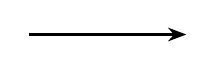
\begin{tikzpicture}[baseline=-0.5ex] \definecolor{tempcolor}{HTML}{000000} \draw[tempcolor,-Stealth,thick] (1,0.0) -- (3,0.0); \end{tikzpicture} & predefined arrow (defined by underlying tree) \\
     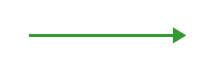
\begin{tikzpicture}[baseline=-0.5ex] \definecolor{tempcolor}{HTML}{339933} \draw[tempcolor,-Triangle,thick] (1,0.0) -- (3,0.0); \end{tikzpicture} & correct directed link across families (skeleton TP, arrow TP, arrow TN) \\
     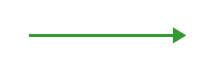
\begin{tikzpicture}[baseline=-0.5ex] \definecolor{tempcolor}{HTML}{339933} \draw[tempcolor,-Triangle,thick] (1,0.0) -- (3,0.0); \end{tikzpicture} & correct directed link within family (skeleton TP, arrow TN) \\
     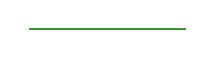
\begin{tikzpicture}[baseline=-0.5ex] \definecolor{tempcolor}{HTML}{339933} \draw[tempcolor,thick]    (1,0.0) -- (3,0.0); \end{tikzpicture} & correct undirected link (skeleton TP, arrow TN) \\
     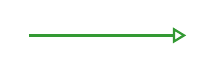
\begin{tikzpicture}[baseline=-0.5ex] \definecolor{tempcolor}{HTML}{339933} \draw[tempcolor,-{Triangle[open]},thick] (1,0.0) -- (3,0.0); \end{tikzpicture} & spurious arrow within family (skeleton TP, arrow FP) \\
     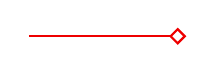
\begin{tikzpicture}[baseline=-0.5ex] \definecolor{tempcolor}{HTML}{ee0000} \draw[tempcolor,-{Turned Square[open]},thick] (1,0.0) -- (3,0.0); \end{tikzpicture} & inverted arrow on correct link (skeleton TP, arrow FP, arrow FN) \\
     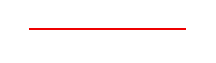
\begin{tikzpicture}[baseline=-0.5ex] \definecolor{tempcolor}{HTML}{ee0000} \draw[tempcolor,thick]    (1,0.0) -- (3,0.0); \end{tikzpicture} & missing arrow on correct cross-family link (skeleton TP, arrow FN) \\
     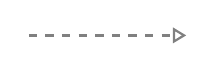
\begin{tikzpicture}[baseline=-0.5ex] \definecolor{tempcolor}{HTML}{808080} \draw[tempcolor,-{Triangle[open]},thick] (1,0.0) -- (3,0.0) [dashed]; \end{tikzpicture} & spurious directed link (skeleton FP) \\  
     \begin{tikzpicture}[baseline=-0.5ex] \definecolor{tempcolor}{HTML}{808080} \draw[tempcolor,thick]    (1,0.0) -- (3,0.0) [dashed] ; \end{tikzpicture} & spurious undirected link (skeleton FP) \\     
     \begin{tikzpicture}[baseline=-0.5ex] \definecolor{tempcolor}{HTML}{c0c0c0} \draw[tempcolor,-{Triangle[open]},thick] (1,0.0) -- (3,0.0) [dotted] ; \end{tikzpicture} & missing directed link (skeleton FN) \\
     \begin{tikzpicture}[baseline=-0.5ex] \definecolor{tempcolor}{HTML}{c0c0c0} \draw[tempcolor,thick]    (1,0.0) -- (3,0.0) [dotted] ; \end{tikzpicture} & missing undirected link (skeleton FN) \\
     \hline
   \end{tabular}
   }
   \caption{Summary of combined color, line style and shape coding used in evaluation graphs}
   \label{eval-graph-colors}
 \end{figure}
 
 After a quick summary of the result for each case study, I will mostly focus on individual cases of red and spurious links, and go into the details of the computation to elucidate why this variant of PLFI failed on these links. These investigations will help to get a full picture of why PLFI is not a perfect method, and lead to some ideas for possible future improvements beyond the current state.
 
 \subsubsection{Case study 1: the Baltic Sea area}
  \begin{figure}
 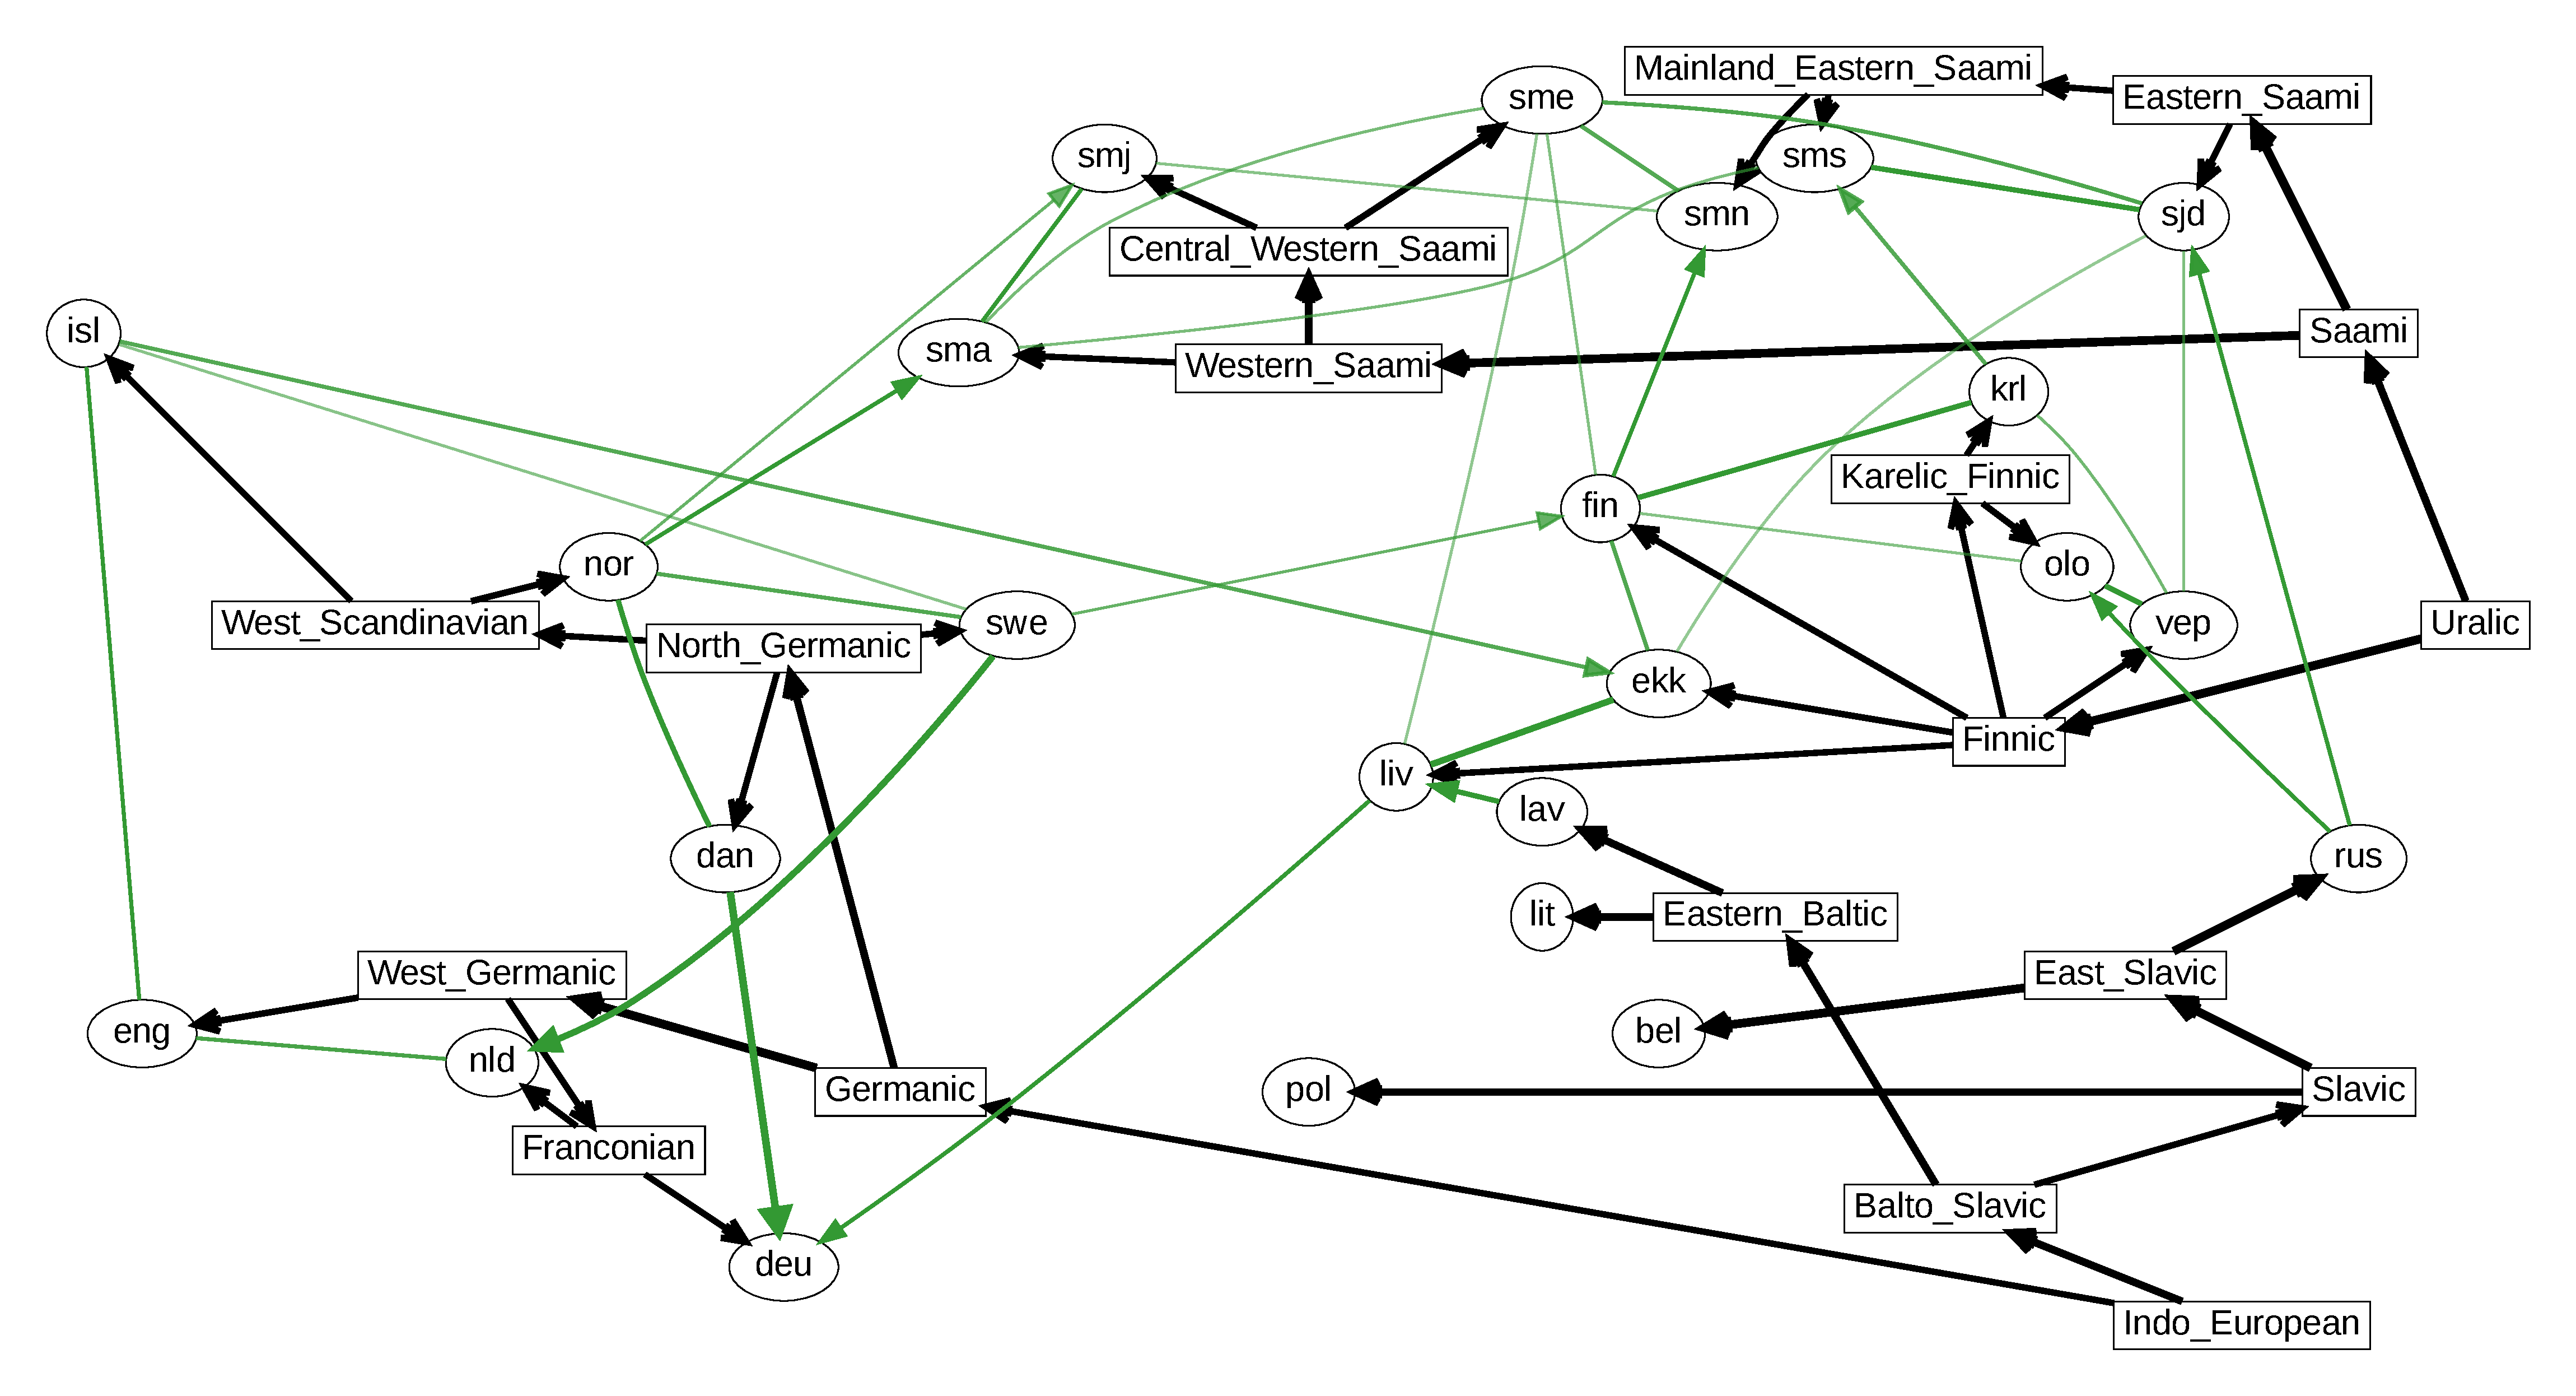
\includegraphics[width=\textwidth]{figures/baltic-fs-ufr-ml-multi.pdf}
 \vspace*{5mm}
 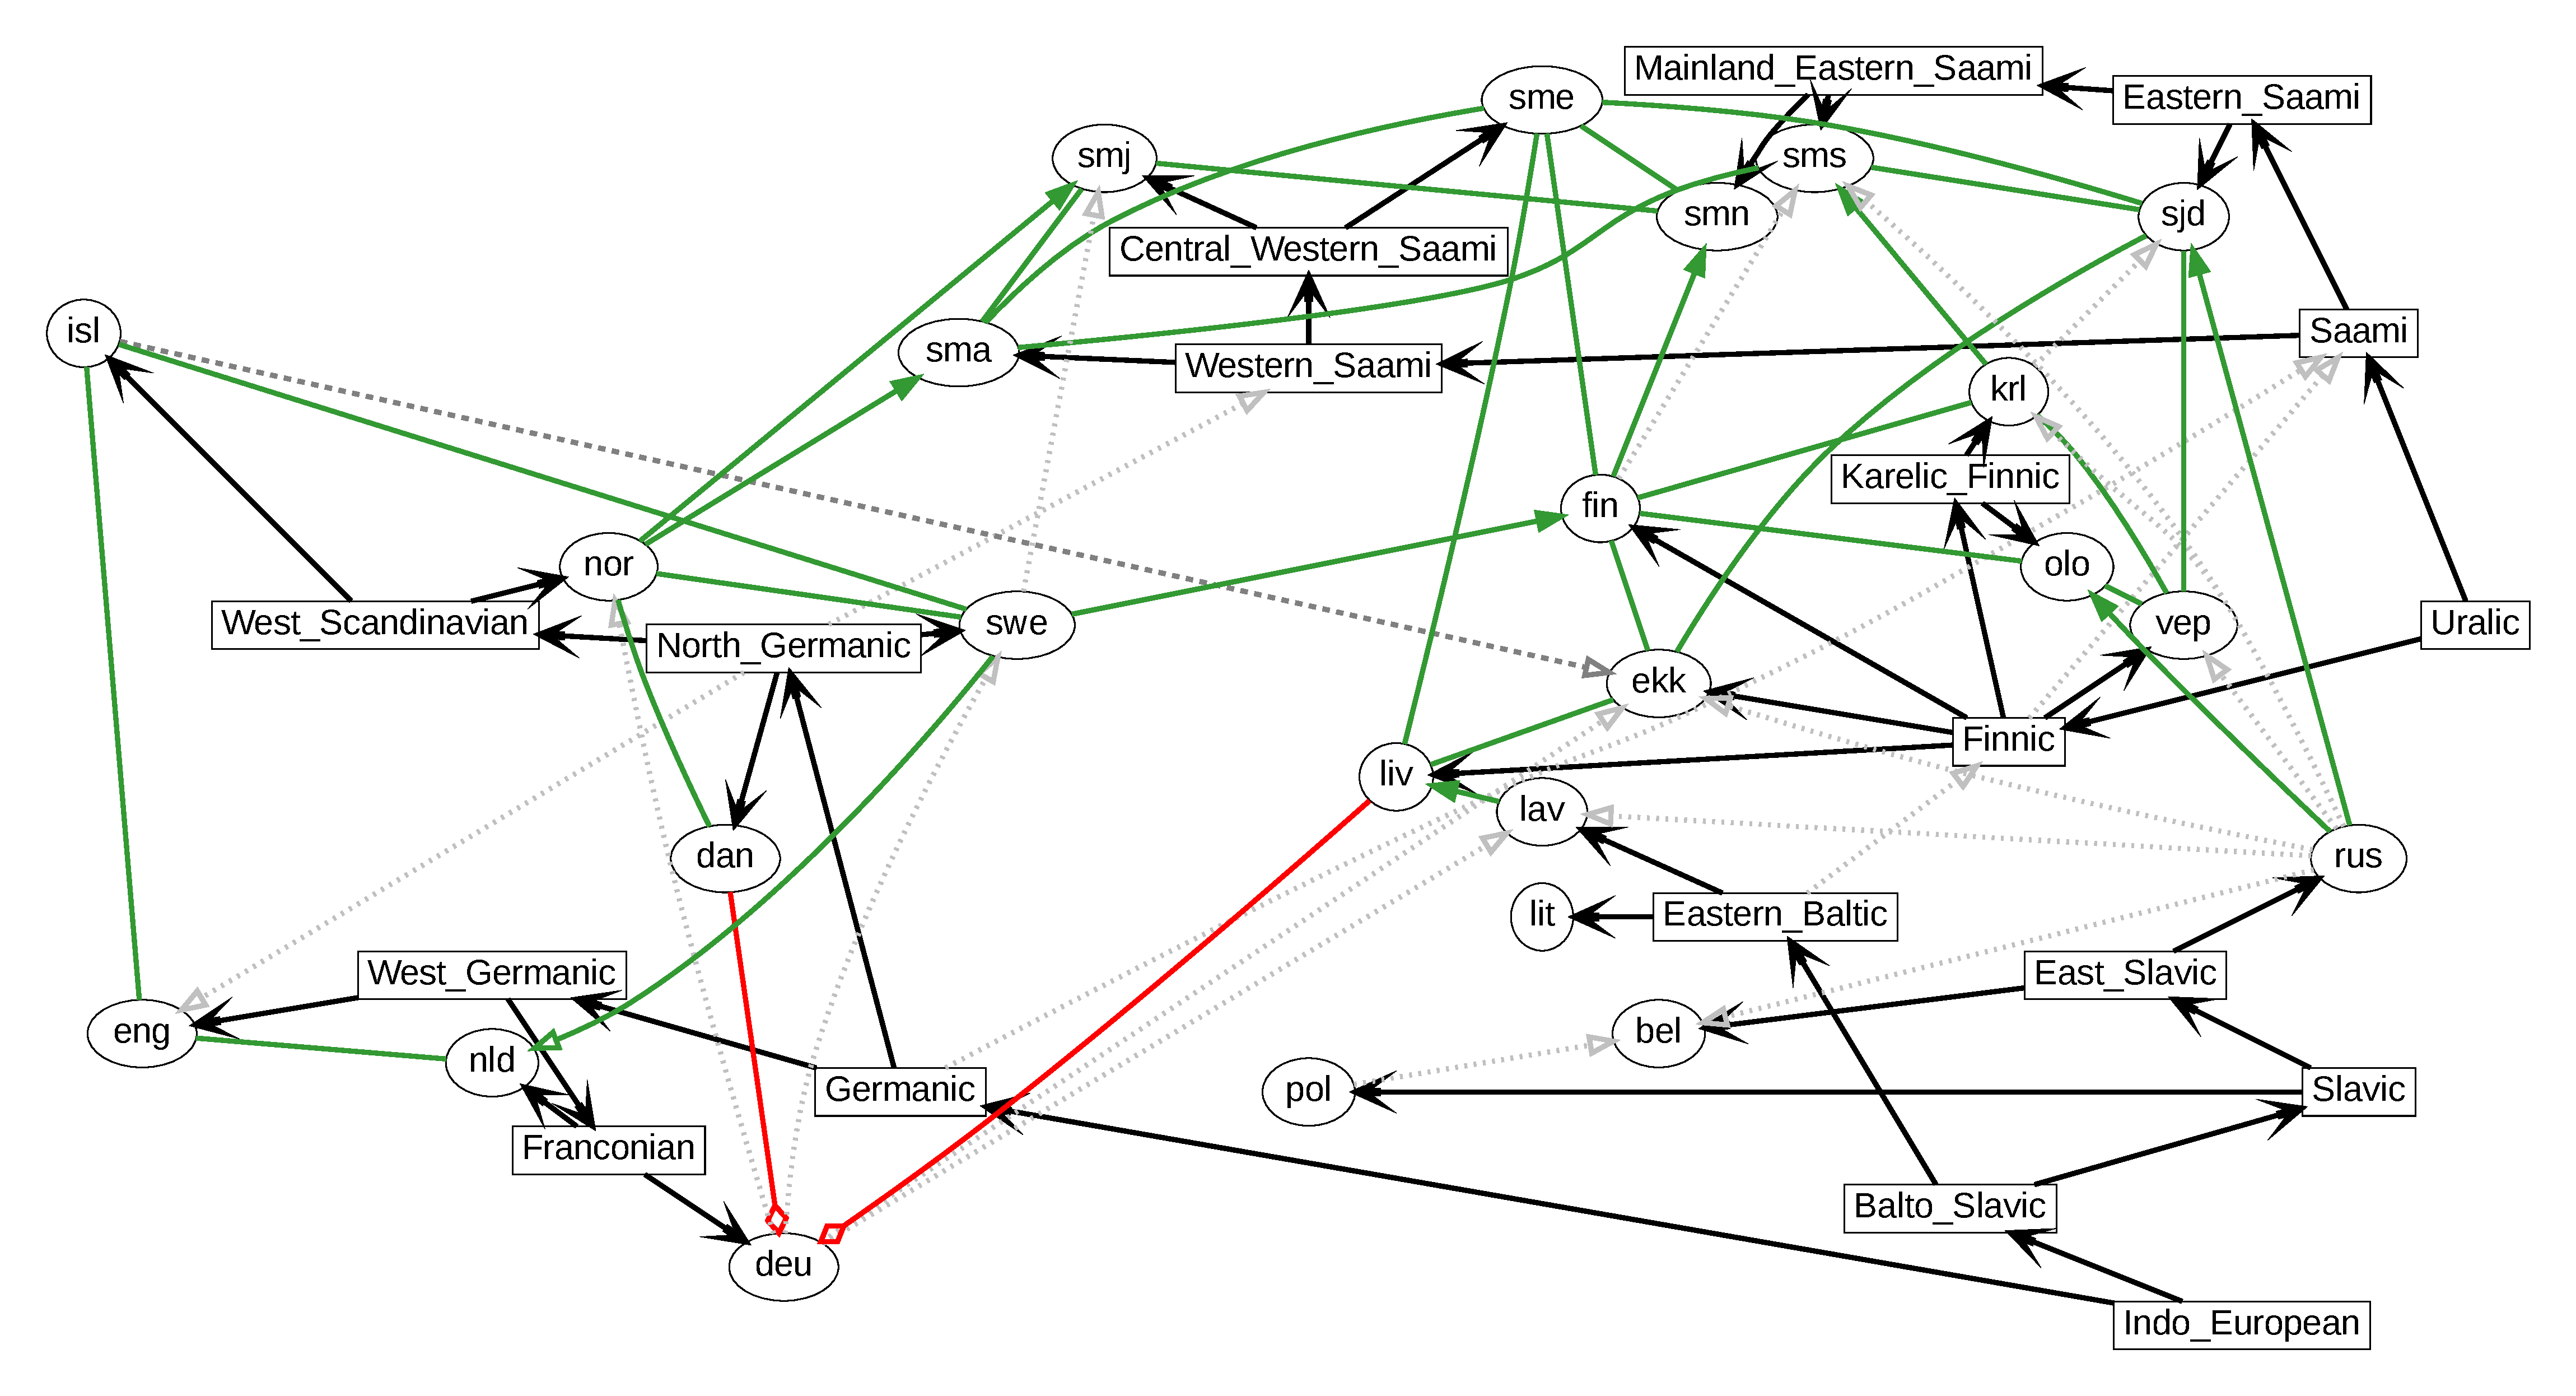
\includegraphics[width=\textwidth]{figures/baltic-fs-ufr-ml-multi-eval.pdf}
 \caption{Result graph (top panel) and evaluation graph (bottom panel) of phylogenetic flow on Baltic Sea data}
 \label{baltic-result-phylo}
 \end{figure}
 Already at first glance, the visualization of results for the Baltic sea case in Figure \ref{baltic-result-phylo} displays only very few errors. The major contacts in the area are all inferred successfully: North Germanic\il{North Germanic languages} influence on Western Saami\il{Western Saami languages} (here imperfectly represented as influence from \ili{Norwegian} on the individual languages), \ili{Russian} influence on all the minority languages on its territory (invisible in the cases of \ili{Veps} and \ili{North Karelian}, due to the mentioned purism of the sources), \ili{Swedish} influence on \ili{Finnish}, and \ili{Latvian} loans in \ili{Livonian}.
 
 Some other influences in the gold standard, such as the Baltic\il{Baltic languages} influence on Finnic\il{Finnic languages} and the Finnic influence on Saami\il{Saami languages}, were not visible in the data, most likely because the multi-value reconstruction these results are based on did not project sufficiently many cognate sets to the level of these proto-languages. This is something we will observe in many cases, due to the cautious reconstructions in this paradigm. Only in graphs derived from single-value reconstructions do the numbers of cognate sets in the ancestral languages become so high that influences between them cannot be explained away completely by their descendants.
 
 Other contacts in the gold standard are imperfectly represented by undirected lateral signals, such as the \ili{German} influence on the continental Scandinavian languages. This is represented by an inverted link from German to \ili{Danish}, whose close relationship with \ili{Norwegian} is recognized, but not as directional, and a second lateral connection involving \ili{Dutch} and \ili{Swedish}. This part of the skeleton could hint at a problem with the language sample in this case study, since much of the German material in Danish and Swedish was actually borrowed from \ili{Low German}, an unobserved language the closest relative to which in our dataset is Dutch. A different problem causes the spurious link from \ili{Icelandic} into \ili{Estonian}. This should actually be another link from German, the Germanic language which by far had the largest lexical influence on Estonian. Now the problem is that some of the material shared with German can be inferred as having flowed through \ili{Livonian}, which contains an even larger share of German loanwords. Some other Germanic words which cannot have travelled via Livonian are present in rather archaic forms in Icelandic, causing most cognates for the remaining overlap to be detected for that language instead of other Germanic languages.
 
 The wrong directionality of the arrow from \ili{Danish} into \ili{German} is simply due to the fact that the unshielded triple $dan \arrowLL deu \arrowLL Franconian$ is detected to be a v-structure due to a very low UFR score of 0.0013. This erroneous low score is due to high overlap of 461 words between Danish and reconstructed Franconian, of which not a single item can be explained only by paths going through German. This is due to the existence of alternative routes, one through inheritance from Germanic, and the other through the Dutch-Swedish connection. We thus have a case where the logic of UFR breaks down due to the complex interplay of path configurations.
 
 Coming to the final inverted arrow $liv \arrowLA deu$, here it is the unshielded triple $lav \arrowLL liv \arrowLL deu$ which does not look like a v-structure at all. This triple has a very high UFR score of 0.6364, caused by the fact that out of the 22 items shared exclusively by \ili{Latvian} and \ili{German} (mostly German loans in Latvian), 21 are also shared by \ili{Livonian}. From the pattern $lav \arrowLA liv \arrowOO deu$ which arises after Latvian influence on Livonian was successfully detected, the propagation rule infers the erroneous link $liv \arrowLA deu$ because otherwise a previously rejected v-structure would have to be assumed. To interpret the result, to the flow model Livonian very much looks like a transmitter of Latvian words into German, after having explained away the contact link from German into Latvian demanded by the gold standard.
 
 To sum up, the two serious mistakes that were produced for this scenario are caused by the fact that the UFR-based v-structure test is not as reliable as it would have to be to guarantee a correct result. As always in constraint-based causal inference, even a single erroneous v-structure test can have strong effects due to propagation. Interestingly, the alternative method TSS has no problem at all to assign the correct directionality to the arrows involving German, once more showcasing the motivation for the alternative method. Since the TSS method makes other mistakes, a way towards avoiding inverted arrows (the worst type of mistake) could be to aggregate the results of both methods, only returning the arrows on which all directionality inference methods agree.
 
 \subsubsection{Case study 2: Uralic and contact languages}
 Moving on to the second case study, we see in Figure \ref{uralic-result-phylo} that while there are a few more problematic arrows, the overall results are still rather convincing. Since the Western part of this case study was already covered by the previous experiment, I will not comment further on the Baltic Sea area here, except for one interesting point. In the absence of \ili{Dutch} from the language set, the West Germanic\il{West Germanic languages} material present in \ili{Swedish} is now inferred as being shared with Standard \ili{German}, the only West Germanic language remaining in the dataset. This highlights one property of the inference method: if relevant languages are not part of the dataset, the method will find the most plausible explanation involving only the attested languages and their recontructed ancestors. The addition or removal of one language can have consequences beyond the immediate vicinity of the language in question, due to alternative routing of lexical flow and changed propagation patterns for directionality information.
 
 Moving to European Russia, we see that the most dominant trend of the region, the pervasive influence of \ili{Russian} on many of the minority languages of the Russian Federation is inferred correctly (dark green arrows pointing outwards from $rus$). The spurious arrows mainly concern inferred secondary influences between branches of Uralic\il{Uralic languages}, on which there is often no consensus among scholars, and which are therefore not represented in my gold standard. For instance, the inferred influence of \ili{Komi} ($koi$) on \ili{Khanty} ($kca$) is not implausible at all, and neither is Khanty influence ($kca$) on \ili{Mansi} ($mns$). On the other hand, most of the long-distance arrows are clearly spurious, such as influence of \ili{Estonian} ($ekk$) on \ili{Hungarian} ($hun$), and of \ili{Erzya} ($myv$) on Mansi ($mns$). Let us inspect a third example, the reconstructed secondary influence of \ili{Udmurt} ($udm$) on \ili{Nganasan} ($nio$), more closely. The reason why the link remains during skeleton inference is legitimate: there is some material shared between Samoyedic\il{Samoyedic languages} and the \ili{Permian languages}, but not the rest of Uralic. The reason why Nganasan and Udmurt were selected to model these lexical isoglosses is again due to the imperfect nature of the cognate detection. All the other Samoyedic languages have undergone much more disruptive sound change than Nganasan, causing the system to find more cognates between the more conservative Nganasan and the other Uralic languages. To a lesser extent, the same pattern applies on the Permian side, where Udmurt has undergone fewer sound changes than Komi. Finally, the erroneous arrow is caused by the fact that according to the UFR criterion, the Erzya ($myv$) lexicon does not look like a mixture of Russian and Udmurt, and neither does Udmurt form a v-structure with Erzya and Nganasan, causing the arrow from Russian into Erzya to be propagated by the principle of avoiding additional v-structures.
 
 While a connection of \ili{Romanian} ($ron$) with \ili{Bulgarian} ($bul$) is inferred correctly by skeleton inference, the directionality of influence between the two languages is inferred to be the opposite of the real situation, where the Romanian lexicon is an obvious mixture of Slavic and Romance elements. The problem here is that Romanian is the only Romance language\il{Romance languages} in the dataset, meaning that on the reduced skeleton, the mixed character of the Romanian lexicon would have to be detected from a v-structure \textit{Indo-European} $\arrowLA ron \arrowAL bul$ with Bulgarian or some other Slavic language\il{Slavic languages}. The UFR score for this triangle is rather close to zero at 0.0340, but not close enough for our empirically determined threshold. An additional Romance language in the dataset would yield a much cleaner v-structure $Romance \arrowLA ron \arrowAL bul$, whereas too little of the Romance material in $ron$ can be reconstructed for \textit{Indo-European}.
 
 A second interesting area where some problems of the method become visible is the interaction between the Turkic\il{Turkic languages} and Uralic languages of the Volga region. The inferred network displays some shared material between \ili{Chuvash} ($chv$) and the two \ili{Mari languages} ($mrj$ and $mhr$), but cannot decide on the directionality of either connection. According to the gold standard, there should be arrows from Chuvash into both Mari languages, but this presupposes that $mrj \arrowLA chv \arrowAL mhr$ is not a v-structure. Unfortunately, a v-structure is exactly what we get by the UFR criterion, since on the rather dense skeleton, transmission via $chv$ is not needed to explain even a single item shared between $chv$ and both variants of Mari, as all of these are projected up to Proto-Mari. Here, the fact that local criteria are used is really showing its negative consequences, because nothing forces the model to explain how this Turkic material ended up in Proto-Mari, which is independent of any Turkic influence conditioned on its two descendants.
 
 A larger part of the Turkic element in \ili{Meadow Mari} ($mhr$) is wrongly attributed to influence from \ili{Bashkir} ($bak$), as it is correctly inferred for \ili{Udmurt}. As the orange color indicates, this is a problem of skeleton inference. Here, the reasons can be traced back to the fact that cognacy data are too coarse-grained to distinguish between different closely related donor languages. While Chuvash and Bashkir are not very closely related, their divergence has primarily happened on the phonetic level, which is not visible in the inferred cognacy data. Taking a look at the actual forms, it instantly becomes clear that Chuvash has been the main source of Turkic material in Mari, but this fact is hidden by the cognate set abstraction. A future improved measure of conditional mutual information which is computed from phonetic distances (see Section 6.1.1) could prove superior here.
 
 While skeleton inference performed with good overall precision, the one truly inexplicable link remaining in the inferred skeleton is the connection between the Balto-Slavic and Samoyedic proto-languages. Inspecting the cognate sets the distribution of which is explained by flow on the spurious link, we see that it mainly consists of Balto-Slavic cognate classes for concepts like \textsc{apple} and \textsc{cat}. As Russian loanwords, these cognate classes are also present in a majority of \ili{Samoyedic languages}, causing them to be reconstructed for the proto-language. It is unclear how this effect can be avoided in general, and how the system could successfully infer that a widespread cognate class in a minority language family might be due to separate borrowings from the majority language, without predetermining the desired result by explicitly modeling which languages are majority and minority languages. This problem is going to become even more visible in the Siberian case study.
 
\begin{sidewaysfigure}
 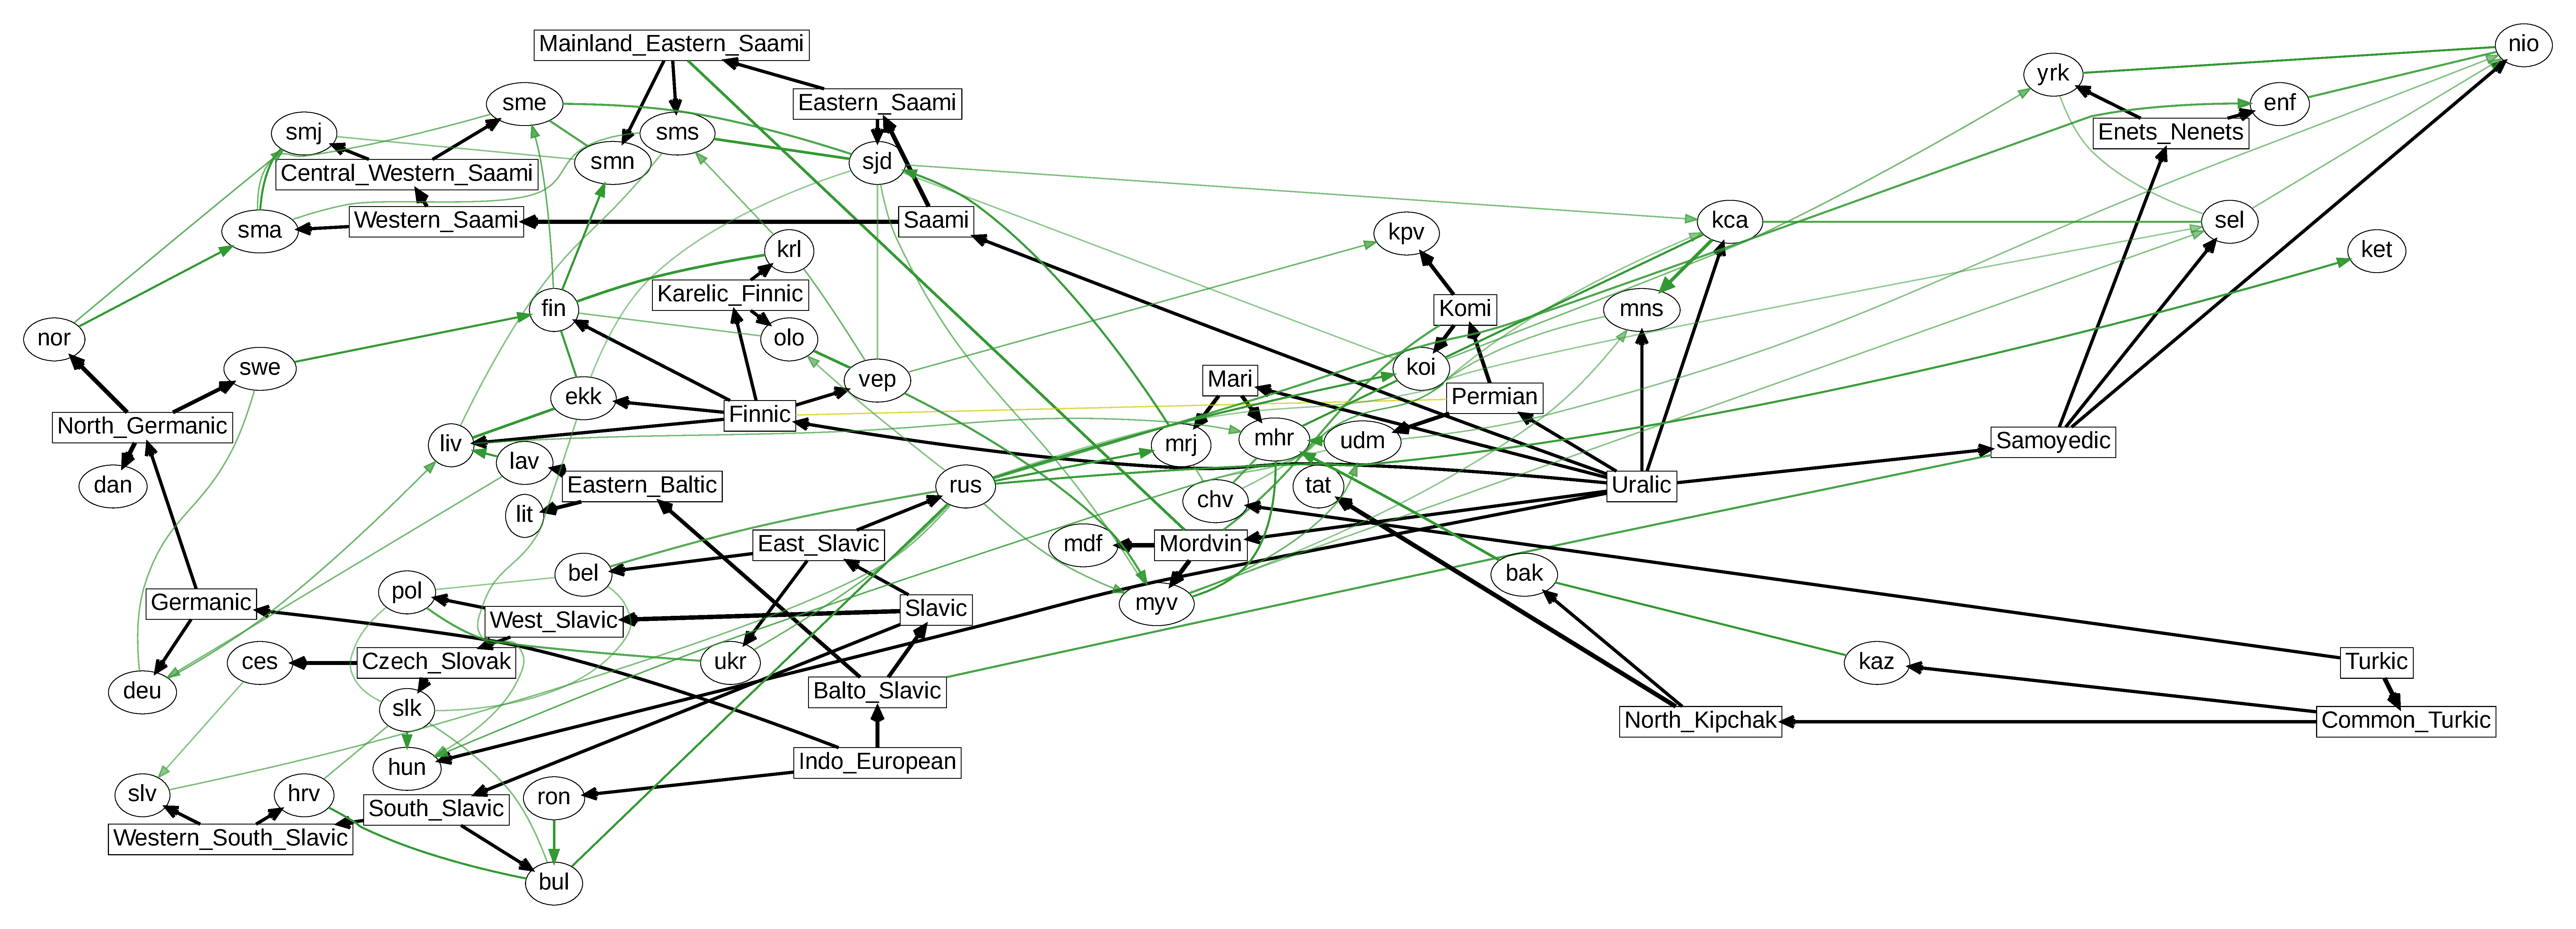
\includegraphics[width=\textwidth]{figures/uralic-fs-ufr-ml-multi.pdf}
 \vspace*{5mm}
 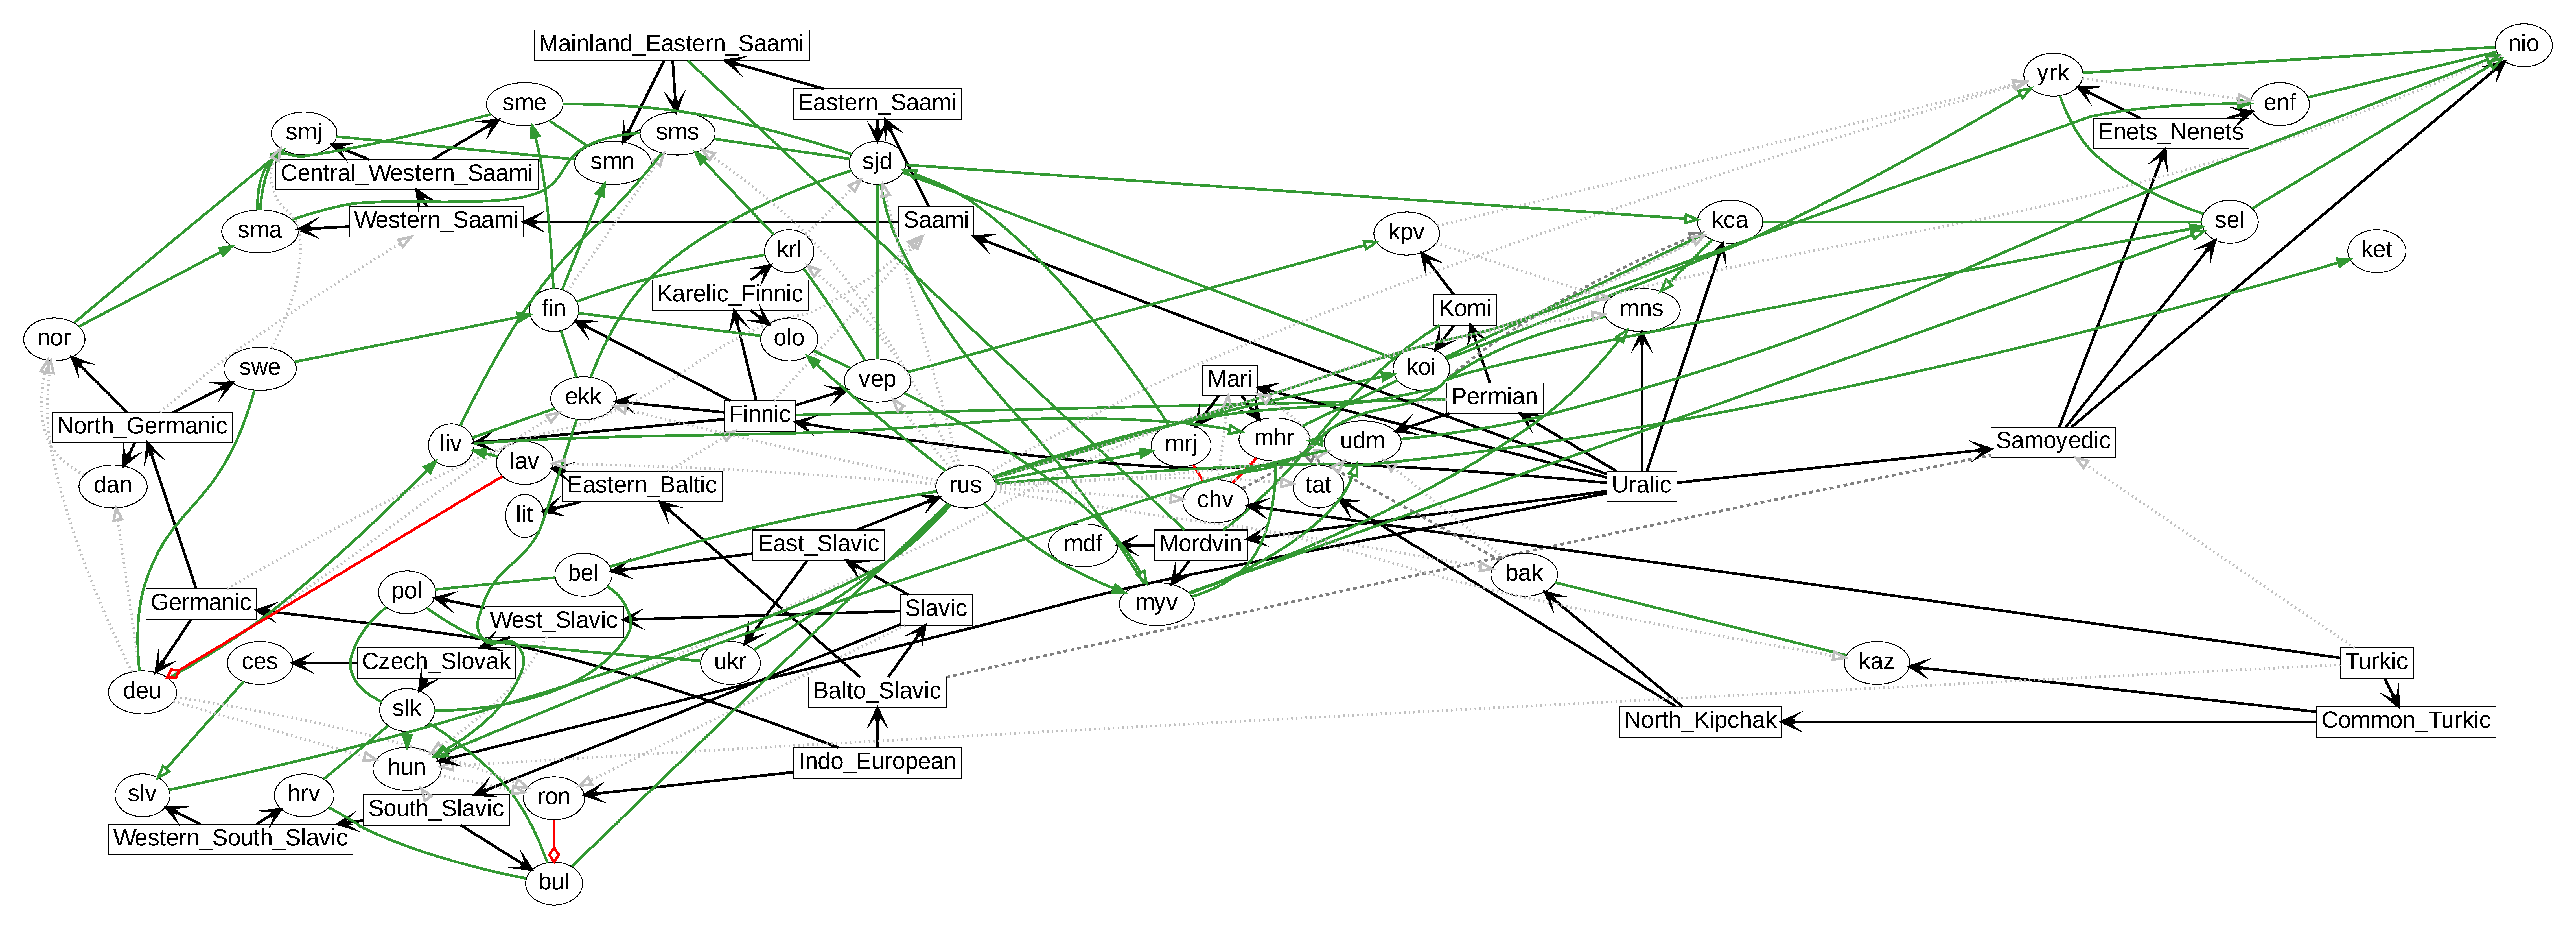
\includegraphics[width=\textwidth]{figures/uralic-fs-ufr-ml-multi-eval.pdf}
 \caption{Result and evaluation of phylogenetic flow on Uralic data}
 \label{uralic-result-phylo}
 \end{sidewaysfigure}
 
 \subsubsection{Case study 3: the linguistic landscape of Siberia}
 The Siberian data display the same large-scale pattern which we already saw in European Russia: all the minority languages have borrowed much of the vocabulary for modern life from \ili{Russian}. As desired, this pattern also appears as the dominant feature of the linguistic area in the inferred lexical flow network visualized in Figure \ref{siberia-result-phylo}. However, two of the arrows, the ones from Russian to \ili{Sakha} ($sah$) and \ili{Evenki} ($evn$), do not have the desired direction. Again, the reason lies in incorrect results of v-structure tests. The triangle $bua \arrowLL sah \arrowLL rus$ does not look at all like a v-structure, because a very large part of the material shared between Russian and \ili{Buryat} ($bua$) is also shared with Sakha, to the point where in a similar pattern to the German-Livonian problem discussed before, conditioning on Sakha actually screens off Russian from Buryat. Due to the failed v-structure test, the correct arrow from Buryat into Sakha is propagated into Russian. The other failed test is for the v-structure $Tungusic \arrowLA evn \arrowAL rus$, which again misses the UFR criterion, albeit at a rather low UFR score of 0.057. Since the inheritance from Tungusic\il{Tungusic languages} is fixed, the only way to resolve this triple in such a way that no v-structure arises, is again by inferring an arrow into Russian.
 
 Coming to the spurious connections, the influence of \ili{Russian} on the two \ili{Yukaghir languages} was detected as going into Proto-Yukaghir, again because of the impossibility for the reconstruction algorithm to decide that a cognate class appearing in both daughter languages should not be projected to the proto-language. Assuming two separate arrows into the two individual languages is simply not the parsimonious solution if we do not include the knowledge that Proto-Yukaghir had already ceased to exist when the Yukaghirs were colonized. Exactly the same problem also leads to the spurious connections between Russian and Proto-Chukotko-Kamchatkan\il{Chukotko-Kamchatkan languages} as well as between Russian and Eskimo-Aleut\il{Eskimo-Aleut languages}.
 
 An erroneous v-structure $sah \arrowAA xal \arrowAL kaz$ is inferred due to zero unique flow between the \ili{Turkic languages} across the Mongolic language $xal$\il{Kalmyk}, indicating that the true pattern $sah \arrowAL xal \arrowAL kaz$ is very unlikely. In fact, the inferred configuration is not as incorrect as the evaluation criteria imply. Arrows between $xal$ and $kaz$\il{Kazakh} in both directions can be justified based on the gold standard, as it includes arrows $Mongolic \arrowLA kaz$ and $Kipchak \arrowLA xal$. The problem can thus be reduced to the fact that $Kipchak$ is not a node in the reduced tree for this scenario, because other Kipchak languages\il{Kipchak Turkic languages} like \ili{Bashkir} and \ili{Tatar} are not part of the language sample.
 
 The spurious connections of \ili{Selkup} ($sel$) to \ili{Chinese} and \ili{Itelmen} are due to a slightly too high noise level in cognate detection. For instance, Selkup and Chinese have an overlap of 28 cognate classes according to the inferred cognacy relation, and the 0.025 threshold would have kicked in at 25 cognate classes. This scenario also provides a nice example for why spurious connections are very problematic, because the Selkup-Chinese connection is also responsible for the inverted arrow from \ili{Japanese} into Chinese, due to an inferred v-structure $sel \arrowLA cmn \arrowAL jpn$. Still, by focusing only on all of these problems one must not forget that in many other cases, PLFI works just as intended, and that many of these errors will disappear under the TSS directionality criterion, again making the case for a combined approach to enhance stability.
 
\begin{sidewaysfigure}
 
\includegraphics[width=0.8\textwidth]{figures/siberia-fs-ufr-ml-multi.pdf}
 \vspace*{5mm}
 
\includegraphics[width=0.8\textwidth]{figures/siberia-fs-ufr-ml-multi-eval.pdf}
 \caption{Result and evaluation of phylogenetic flow on Siberian data}
 \label{siberia-result-phylo}
\end{sidewaysfigure}

\subsubsection{Case study 4: a visit to the Caucasus}
With the Caucasus scenario, we finally encounter the most complex test case. As can be seen on visual inspection of the evaluation graph in Figure \ref{caucasus-result-phylo}, the more peripheral influences from \ili{Arabic} and \ili{Russian} into the Caucasus area are inferred correctly, but in the chaotic situation among Caucasian languages, there is just too much interacting and contradictory signal for PLFI to perform well.
 
The problems within Daghestanian\il{Daghestanian languages} might also be due to imperfections in the gold standard (the Caucasus being the only region where it was almost impossible to find literature on language contacts for some languages), but the case of \ili{Georgian} ($kat$), an isolate in this dataset, points to a further issue that requires some consideration.
 
The underlying signal indicating language contact always comes in the shape of cognate classes present in some child language of an ancestral language which does not contain them, but a more distant language does. This is the pattern which makes the data non-tree-like, and causes lateral connections that cannot be explained away. Now, the directionality inference can recognize that the recipient language is a mixture of its own ancestor and the donor language. This entire mechanism cannot work reliably for isolated languages, because there is no proto-language in the model, and if we assumed an additional proto-language representing an earlier stage of the isolate, the reconstruction algorithm could not decide based on the single descendant language which cognate classes must have existed at that node, and would project all the inherited material up into the proto-language. The only reason why the arrow from Russian into the Siberian isolate Ket was inferred successfully in the previous case study was the 
other erroneous arrow from Sakha into Russian. This problem only occurs among isolates, however. An additional Slavic language in the dataset would have shared most of the Russian loans as well, and Proto-Slavic would have provided the necessary third language for a negative collider test involving the link from Ket into Russian. In a sense, the method faces the same limitations which historical linguists face when trying to infer the directionality of loans between isolates. This is notoriously difficult to do, and can only be done when loanwords are recognizable due to language-internal reasons, e.g.\ because they do not adhere to some phonological constraints governing the rest of the lexicon.
 
Finally, let us investigate the reason why the important connections $tur \arrowLA kmr$ and $pes \arrowLA tur$ could not become part of the skeleton. The reason is that with \ili{Azeri} ($azj$), there is another Turkic language that is lexically very close to \ili{Turkish}, but has interacted with both \ili{Iranian languages} even more, because of lexical contact on a more equal footing with \ili{Kurdish} as minority languages of Iran. The overlap of Azeri with \ili{Persian} and Kurdish therefore subsumes the overlaps of both languages with Kurdish, leaving only the links with Azeri in the skeleton. The signal behind the spurious arrow from Azeri into Kurdish is actually the one which should have created the missing arrow from Turkish into Kurdish.
 
Finally, let us explore why the nature of \ili{Azeri} and \ili{Uzbek} as \ili{Turkic languages} with many \ili{Persian} loans is not understood by the algorithm, which instead produces the wrongly directed arrows $azj \arrowLA pes$ and $uzn \arrowLA pes$. Here, Persian is the language which looks like a mixture of elements of Azeri and Uzbek, the assumed transmitted material being exactly the Persian loans the two Turkic languages share, because these are projected into and then explained by Turkic. On a more abstract level, this phenomenon is another example of how the indistinguishability of inherited words and widespread loans can result in erroneous arrows. Unlike other erronous v-structures, this is purely a reconstruction problem which also hits the TSS criterion, where the arrow $uzn \arrowLA pes$ has an evidence ratio of $3.575$. In the global NorthEuraLex network, this problem does not occur, because the many other Turkic languages untouched by Persian produce a Turkic reconstruction that does not 
contain any of these. The situation could therefore be improved by considering more Turkic languages. It is an interesting question whether to a historical linguist, all the Persian elements in Turkish and Uzbek would actually be recognizably foreign if only three Turkic languages were attested.
 
  \begin{figure}[ht!]
 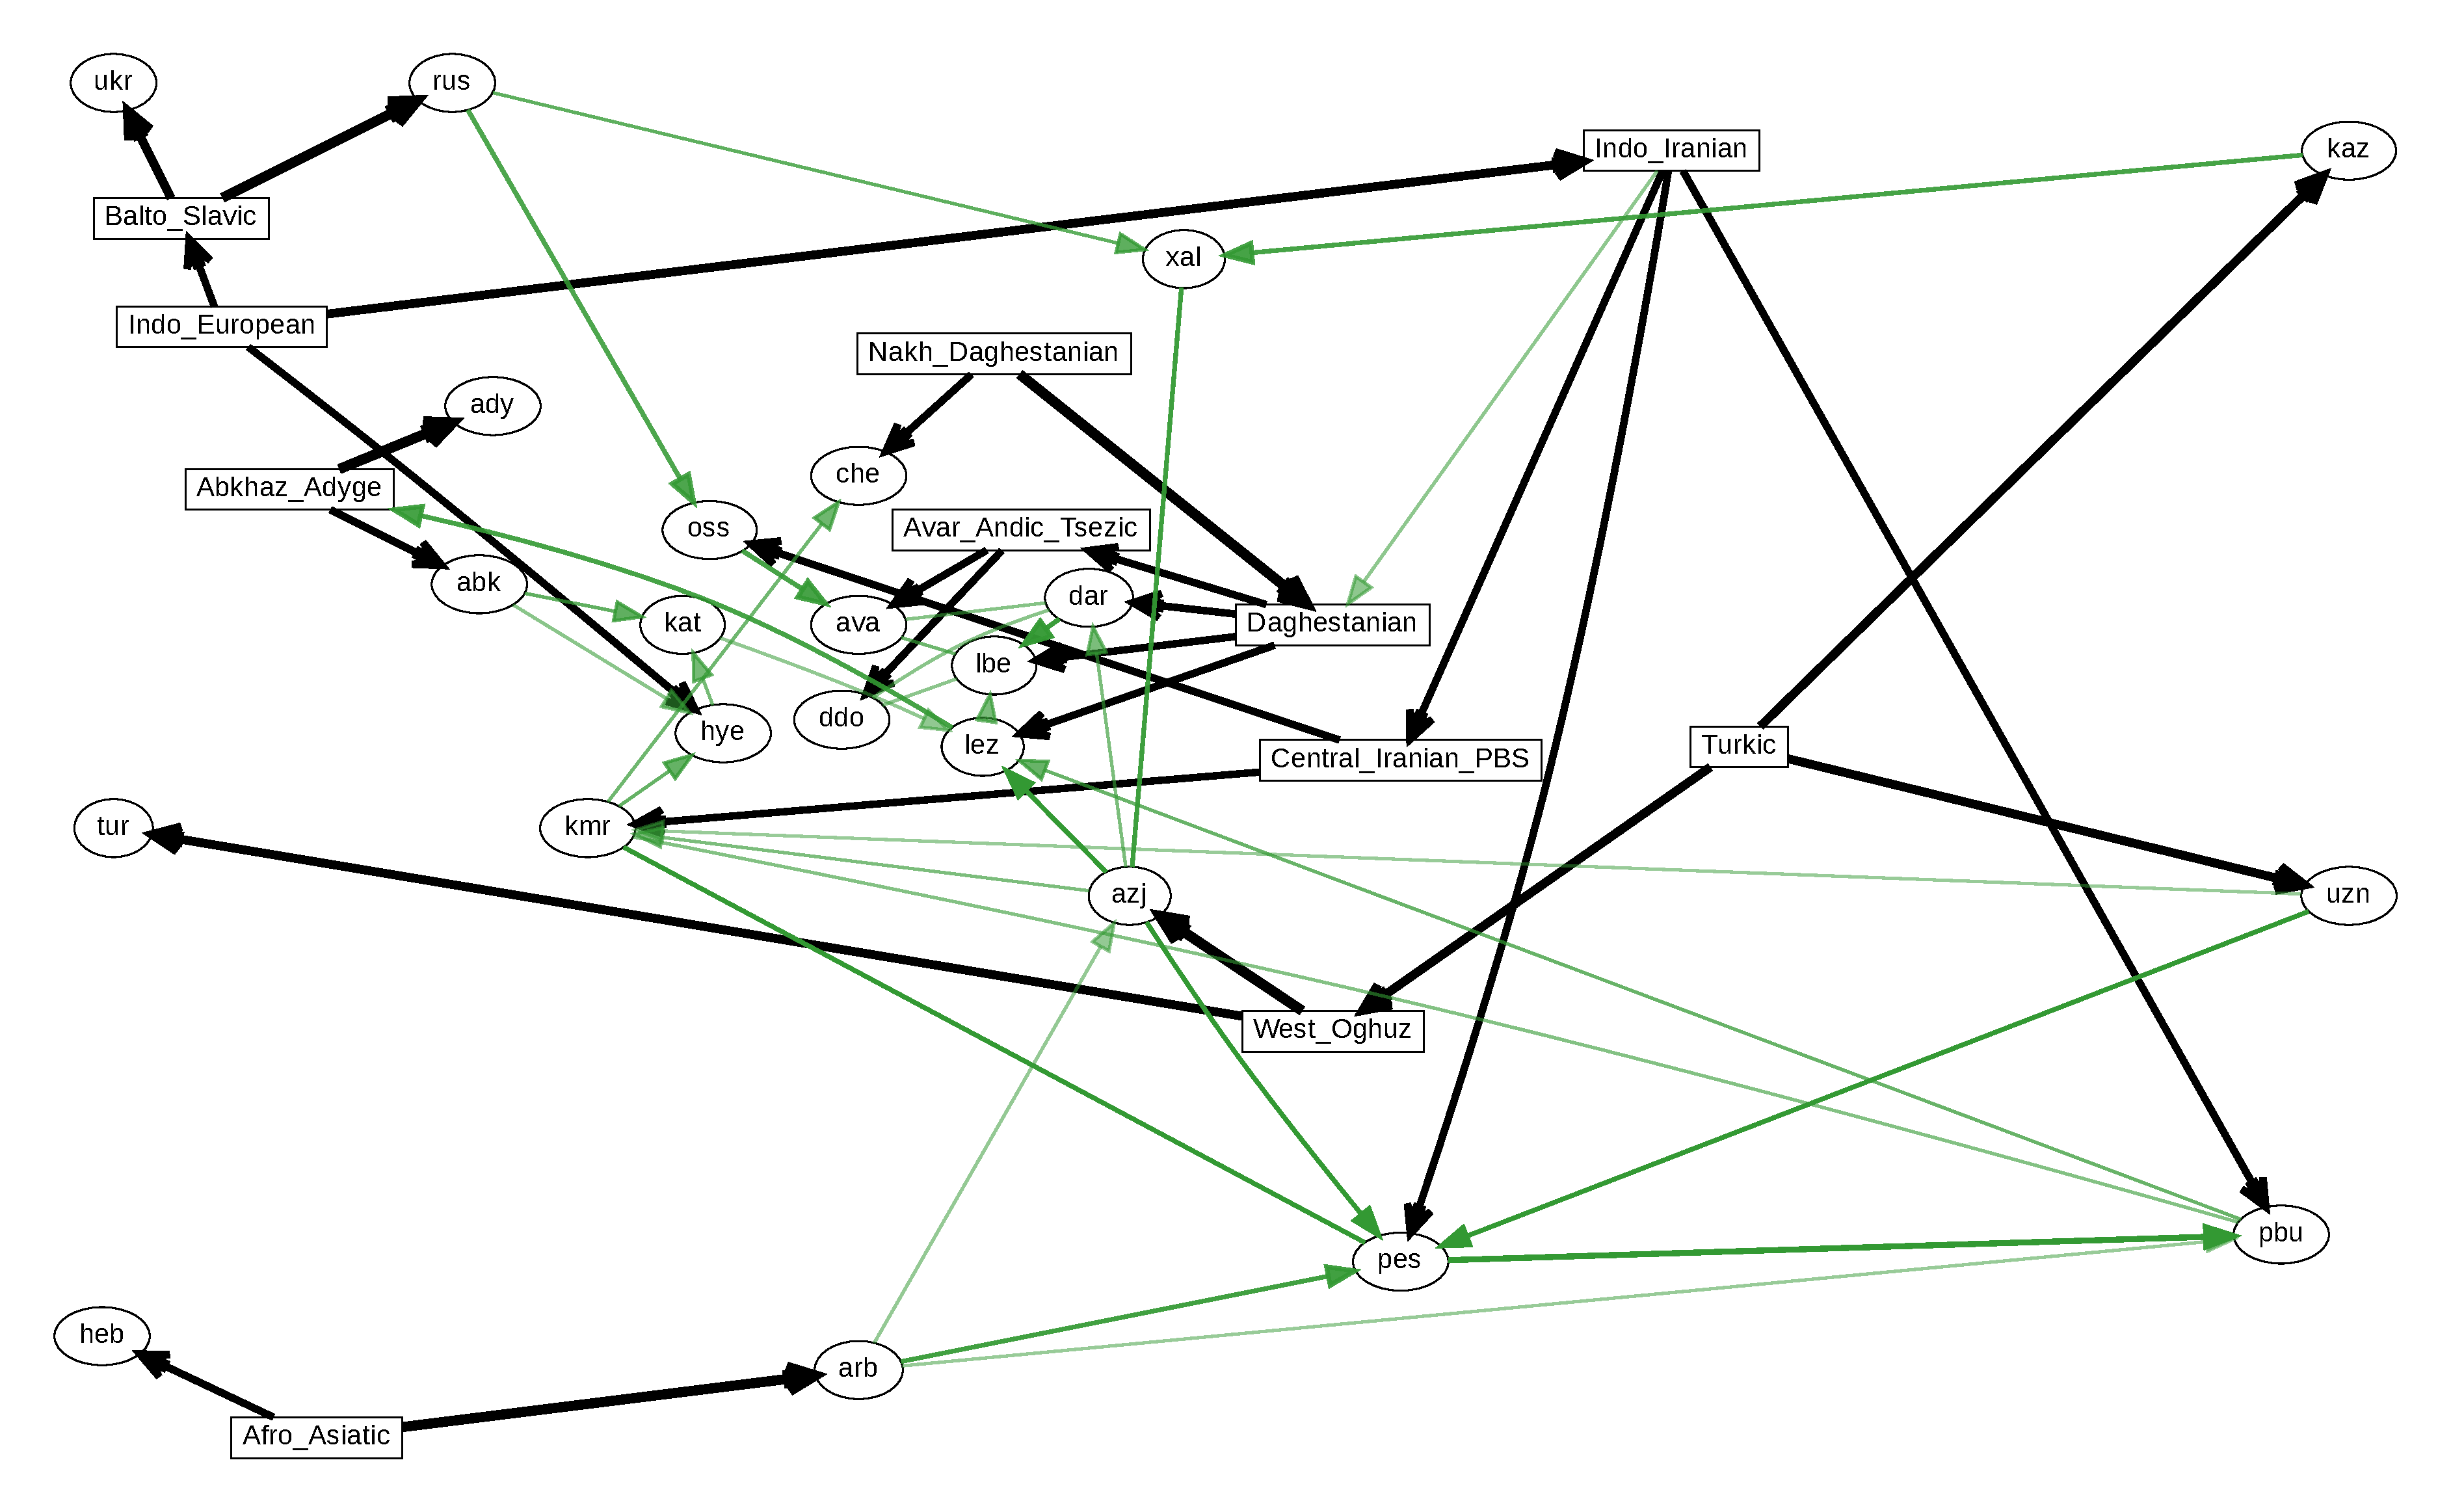
\includegraphics[width=\textwidth]{figures/caucasus-fs-ufr-ml-multi.pdf}
 \vspace*{5mm}
 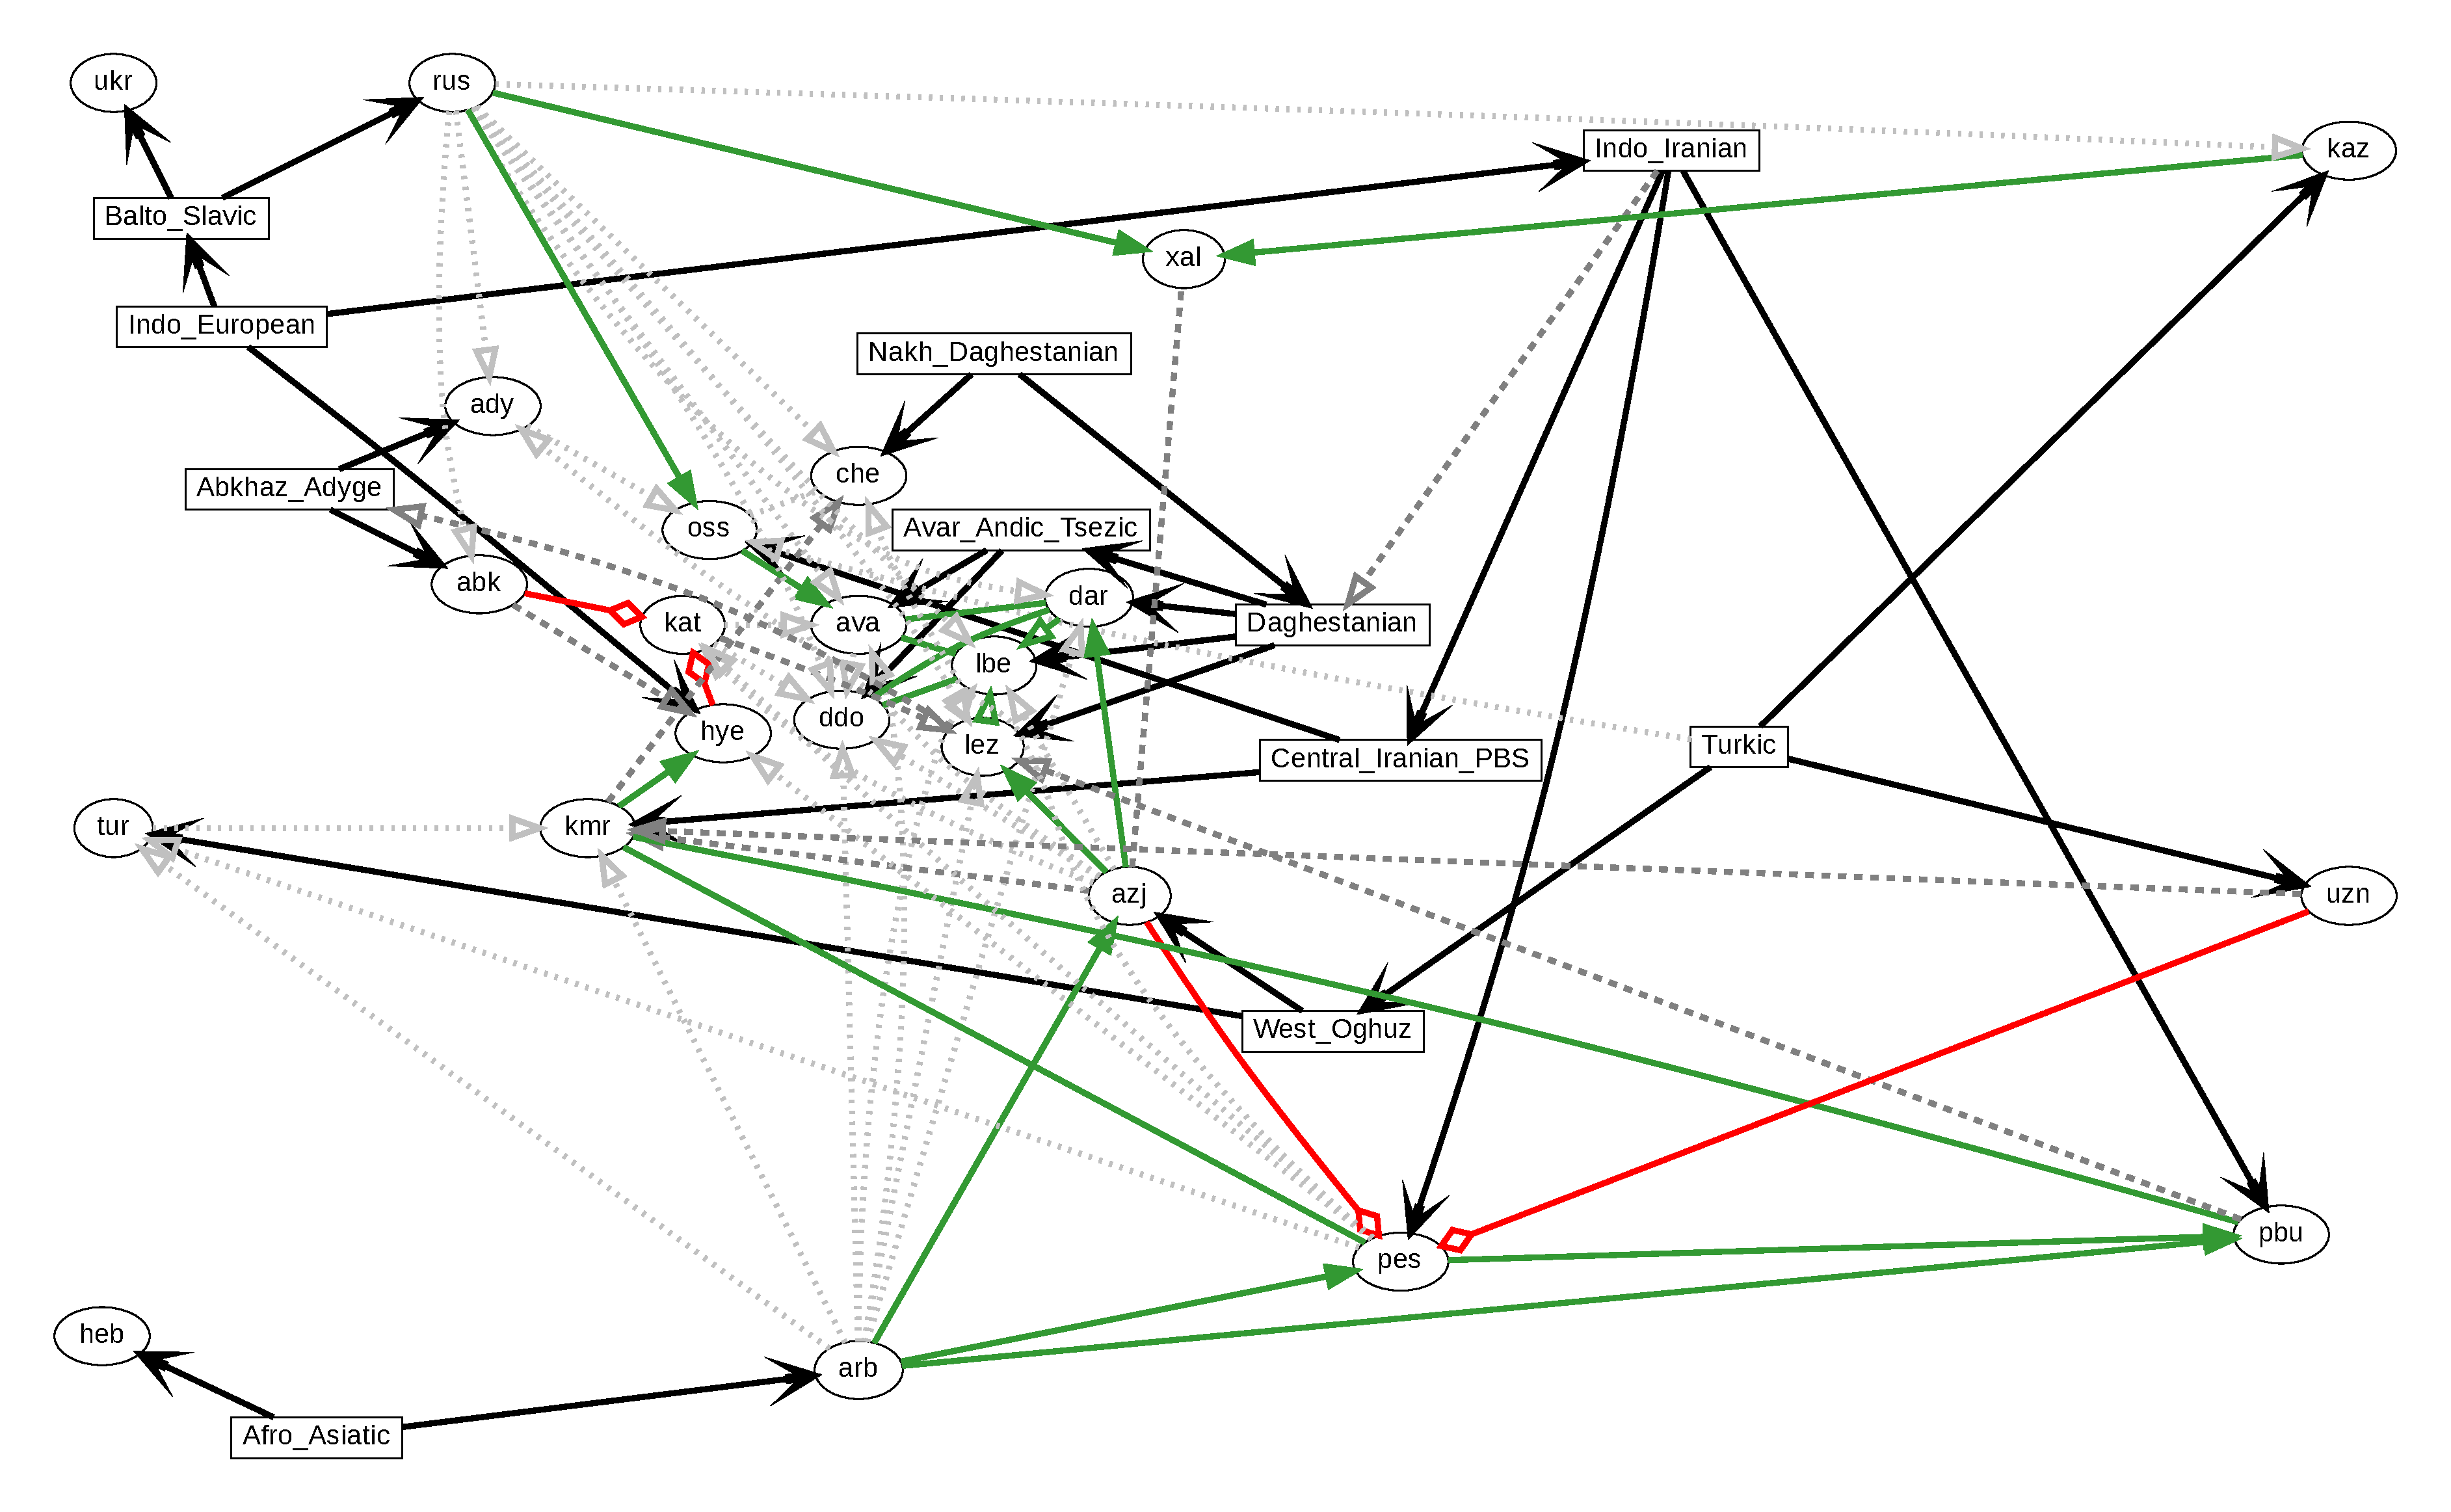
\includegraphics[width=\textwidth]{figures/caucasus-fs-ufr-ml-multi-eval.pdf}
 \caption{Result and evaluation of phylogenetic flow on Caucasian data}
 \label{caucasus-result-phylo}
 \end{figure}

\subsection{Evaluation on simulated data}
As the final analysis in this chapter, we now return to the simulated data. There are two important questions answers to which the simulated data will help us find. First, we want to quantify how much potential performance we lost by using ancestral state reconstruction methods and acting as if the reconstructed data were actually observed. Second, we want to know whether the performance on the simulated data is comparable to what we observed on NorthEuraLex, and whether our previous findings about the relative advantages of the different skeleton and directionality inference methods generalize beyond my dataset.

We start by comparing the skeleton performance measures for the three skeleton inference methods on the perfect data (i.e.\ the picture we get if we take the actual states of the simulation when the proto-languages split) to the results on the two best reconstructions. The results are given in Table \ref{perfect-vs-reconstruction-skeleton}. If the best skeleton inference method is picked on both types of data, we see an only moderate decrease in F-score from about 87\% to 79\% for the more exact single-value reconstruction, and to 74\% for the more generous multi-value reconstruction. Precision and recall suffer about equally, showing that the reconstructed data contain a more noisy version of the same signal. We see that a good reconstruction method can help us a long way towards results comparable to what we would get on perfect data, confirming our impression that it is possible in principle to extract information about historical language contacts from a cognacy-encoded dataset covering only their living 
descendants. Interestingly, while flow-separation methods worked best for the NorthEuraLex data, the performance of PS is comparable on perfect data, and even superior on the reconstructed data, especially due to a much higher recall at comparable precision. Interpreting this result, erroneous reconstructions appear to have a rather strong effect on the reliability of connecting paths, indicating that while not clearly superior on perfect data, on noisy reconstructions the PS variant is surprisingly robust.

\begin{table}
 \centering
  \begin{tabular}{cccc}
  \hline \hline
  \# & PrfPC & PrfPS & PrfFS\\ \hline
  skPrc & \textbf{0.901} & 0.870 & 0.829\\
  skRec & 0.780 & \textbf{0.915} & 0.915\\
  skFsc & 0.837 & \textbf{0.892} & 0.870\\
  \hline
 \end{tabular}\\[0.5cm]
 \begin{tabular}{ccccccc}
  \hline \hline
  \# & MLsPC & MLsPS & MLsFS\\ \hline
  skPrc & \textbf{0.851} & 0.798 & 0.711\\
  skRec & 0.539 & \textbf{0.722} & 0.659\\
  skFsc & 0.660 & \textbf{0.758} & 0.684\\
  \hline
 \end{tabular}\\[0.5cm]
\begin{tabular}{ccccccc}
  \hline \hline
  \# & MLsPC & MLsPS & MLsFS\\ \hline
  skPrc & \textbf{0.855} & 0.797 & 0.710\\
  skRec & 0.527 & \textbf{0.720} & 0.658\\
  skFsc & 0.652 & \textbf{0.757} & 0.683\\
  \hline
 \end{tabular}
 \caption{Comparing skeleton performance for perfect ancestral data and the two best reconstructions}
 \label{perfect-vs-reconstruction-skeleton}
\end{table}

The consequences of reconstruction vs. observed data for arrow performance are again not easily quantifiable in our framework, because they result in different skeletons. Still, within each variant we can compare the arrow performance resulting from the different directionality inference methods. To maintain comparability with the NorthEuraLex results, only the numbers for the FS method are given in Table \ref{perfect-vs-reconstruction-arrows}. The apparently low arrow performance for the perfect ancestral data is due to the higher skeleton recall, which leaves many weak links in the skeleton where overlaps are small and directionality evidence therefore uncertain.

Instead, these numbers provide us with a further piece of the answer to the second question. Contrary to what we saw on the NorthEuraLex dataset, TSS directionality can now compete with the UFR criterion across reconstructions. The theoretical considerations leading to the TSS method seem to apply much better on this dataset. So what is the underlying reason? The only obvious difference between the two types of scenarios is that the simulated data have perfect cognate clustering, whereas the automated cognate clustering that I performed to derive cognacy overlap data from NorthEuraLex is quite noisy. Essentially, this noise causes non-zero values for $\delta$ even in unshielded colliders, making these more difficult to detect, and preventing the TSS method from reaching its full potential. In contrast, the UFR method can handle noise much better, but as we have seen in the case studies, it tends to run into problems in dense graphs where unshielded triples are rare, which is the case in the Caucasus as well as in many of the simulated scenarios. The fact that the statistical assumptions behind causal inference hold much better for perfect cognacy judgments also shows in the much better performance of the VPC and SPC directionality inference methods on the simulated data. While both were completely useless on noisy cognacy data, on clean cognacy data they do manage to capture some of the signal, although their results remain very unreliable, and the specialized directionality inference methods perform better by a significant margin.

\begin{table}
 \centering
  \begin{tabular}{ccccc}
    \hline \hline
   & \multicolumn{4}{l}{FS on perfect ancestral data}\\ 
   & VPC & SPC & UFR & TSS\\ \hline
  arPrc & 0.414 & 0.362 & \textbf{0.438} & 0.371\\
  arRec & 0.415 & 0.313 & \textbf{0.585} & 0.366\\
  arFsc & 0.414 & 0.336 & \textbf{0.501} & 0.368\\
  \hline
 \end{tabular}\\[0.5cm]
 \begin{tabular}{ccccc}
  \hline \hline
   & \multicolumn{4}{l}{FS on MLsgl reconstruction}\\ 
   & VPC & SPC & UFR & TSS\\ \hline
  arPrc & 0.490 & 0.512 & 0.432 & \textbf{0.555}\\
  arRec & 0.362 & 0.290 & \textbf{0.423} & 0.343\\
  arFsc & 0.417 & 0.370 & \textbf{0.428} & 0.424\\
  \hline
 \end{tabular}\\[0.5cm]
 \begin{tabular}{ccccc}
  \hline \hline
   & \multicolumn{4}{l}{FS on MLmlt reconstruction}\\ 
   & VPC & SPC & UFR & TSS\\ \hline
  arPrc & 0.485 & 0.508 & 0.435 & \textbf{0.561}\\
  arRec & 0.354 & 0.288 & \textbf{0.422} & 0.347\\
  arFsc & 0.409 & 0.368 & 0.428 & \textbf{0.428}\\
  \hline
 \end{tabular}
 \caption{Comparing skeleton performance for perfect ancestral data and the two best reconstructions}
 \label{perfect-vs-reconstruction-arrows}
\end{table}

Again, we can combine skeleton and arrow F-scores by multiplication to derive an overall performance figure for each of the compared methods, which makes it possible to quantify approximately how much overall performance we lose due to reconstruction. The resulting numbers are ranked by the best result on perfect ancestral data in Table \ref{variant-comparison-perfect-vs-reconstructed}, which compares the performance on the two reconstructions against the perfect data, also quantifying the losses or gains in percentages. Overall, the FS-UFR variant is clearly the best-performing on the perfect data, whether FS-TSS is the best on reconstructed data. Moreover, most methods perform between 20\% and 30\% worse on both single-value and multi-value ML reconstruction on the perfect data. Encouragingly, the specialized directionality inference method TSS does not follow the general pattern, but provides a method that at less than 10\% decrease is stable against the negative consequences of reconstruction, and this 
at moderate performance.

\begin{table}
 \centering
 \begin{tabular}{cclrlr}
 \hline \hline
PLFI Variant & perfect data & MLsgl & (diff) & MLmlt & (diff)\\ \hline
\texttt{FS-UFR} & 0.436 & 0.293 & (-32.8\%) & 0.293 & (-32.8\%)\\
\texttt{FS-VPC} & 0.360 & 0.285 & (-20.8\%) & 0.279 & (-22.5\%)\\
\texttt{PS-VPC} & 0.346 & 0.273 & (-21.1\%) & 0.271 & (-21.7\%)\\
\texttt{FS-TSS} & 0.320 & 0.290 & (- 9.4\%) & 0.293 & (- 8.4\%)\\
\texttt{PC-VPC} & 0.313 & 0.232 & (-25.9\%) & 0.237 & (-24.3\%)\\
\texttt{FS-SPC} & 0.292 & 0.253 & (-13.4\%) & 0.251 & (-14.0\%)\\
  \hline
 \end{tabular}
 \caption{Analysis of consequences of reconstructed data for selected PLFI variants}
 \label{variant-comparison-perfect-vs-reconstructed}
\end{table}

Finally, we can compare the combined scores to elucidate to what extent the methods behave similarly on the simulated and the NorthEuraLex data. In Table \ref{variant-comparison-simulated-and-nelex}, the different variants are ranked by their overall performance on the simulated data, and the equivalent figure on the NorthEuraLex data is given for comparison. The difference in percent, plus the rank of each method in the ranking by performance on the NorthEuraLex data, are given in addition to facilitate interpretation of results. Apart from the already mentioned advantage of TSS on simulated data, and of UFR on noisy-cognate data, the methods agree on four of the top-five methods, and the advantage of specialized skeleton and directionality inference techniques persists for the simulated data. This shows that my findings for NorthEuraLex generalize well to the simulated data, validating both the simulation model and the PLFI paradigm.

\begin{table}
 \centering
 \begin{tabular}{lrrrr}
\hline \hline
PLFI Variant & simulated & NorthEuraLex & difference & rank on NELex\\ \hline
\texttt{MLmlt-FS-UFR} & 0.293 & 0.392 & +0.099 & 1\\  
\texttt{MLmlt-FS-TSS} & 0.293 & 0.349 & +0.056 & 2\\
\texttt{MLsgl-FS-TSS} & 0.293 & 0.344 & +0.051 & 3\\
\texttt{MLsgl-FS-UFR} & 0.290 & 0.324 & +0.034 & 4\\
\texttt{MLsgl-FS-VPC} & 0.285 & 0.081 & -0.204 & 9\\
\texttt{MLmlt-FS-VPC} & 0.279 & 0.110 & -0.169 & 6\\
\texttt{MLsgl-PS-VPC} & 0.273 & 0.098 & -0.175 & 8\\
\texttt{MLmlt-PS-VPC} & 0.271 & 0.134 & -0.137 & 5\\
\texttt{MLsgl-FS-SPC} & 0.253 & 0.043 & -0.210 & 11\\
\texttt{MLmlt-FS-SPC} & 0.251 & 0.000 & -0.251 & 12\\
\texttt{MLmlt-PC-VPC} & 0.237 & 0.098 & -0.139 & 7\\
\texttt{MLsgl-PC-VPC} & 0.232 & 0.045 & -0.187 & 10\\
  \hline
 \end{tabular}
 \caption{Comparison of PLFI variants between datasets}
 \label{variant-comparison-simulated-and-nelex}
\end{table}

To summarize my findings, the PLFI paradigm of reconstructing ancestral cognates and treating them as additional observations in a causal inference paradigm has turned out to work reasonably well, although the quality of results depends a lot on the quality of the reconstruction as well as the choices of skeleton and directionality influence algorithms in the causal framework. The most important positive result of the evaluation is that the recall values for the skeleton are high, indicating that if lateral connections exist in the data, they will generally be present in the lexical flow graph. Also, the skeleton precision values indicate that about three quarters of the lateral connections in the graph will turn out to correspond to actual contacts on closer examination. This shows that PLFI lives up to its promise as a promising exploratory tool for historical linguists in the initial stages of clarifying the linguistic history of a region. Directionality inference is less reliable, but we have seen that in scenarios involving the contacts between larger families (and not isolates), about four out of five inferred arrows will have the correct direction. On the downside, deciding whether influences occurred between extant languages or their ancestors turned out to be very difficult and unstable across different reconstructions, which guides us towards the less ambitious contact flow task that will be tackled in the next chapter.

\chapter{Contact lexical flow inference}\label{sec:7}
Having established PLFI as an exploratory tool for detecting directional contact in the linguistic history of a region, we now turn towards the second task which we set out to tackle within the lexical flow framework. After a summary of where we stand after \chapref{sec:6}, and after an overview of what will be different in this chapter, in \sectref{sec:7.2} I explain why the contact flow inference problem has the shape of a causal inference problem with hidden common causes. 

In \sectref{sec:7.3}, I explain why the vanilla RFCI algorithm as introduced towards the end of \chapref{sec:3} for causal inference problems of this shape, is difficult to apply on the basis of noisy cognacy overlap data. \sectref{sec:7.4} describes my most successful attempt to compensate for these weaknesses, which is to define a significance test for v-structure decisions based on a very close connection with the hypergeometric distribution. The resulting variant of the RFCI algorithm is called Contact Lexical Flow Inference (CLFI), and is presented both in pseudocode and as an informal description in \sectref{sec:7.5}. 

\sectref{sec:7.6} evaluates the different CLFI variants resulting from different approaches to skeleton and arrow inference on the same real and synthetic datasets which were already used in the previous chapter. For this purpose, the evaluation metrics have to be adapted to the new problem, and phylum separation is added as a new performance criterion.

An early version of contact flow inference was previously discussed in \cite{dellert2016a}. There, the method was tested on an older version of NorthEuraLex for a language set similar to the current Uralic case study, with promising results which the version presented in this chapter does not significantly improve upon, although it performs better on other case studies.

\section{The contact flow inference task}\label{sec:7.1}
To recapitulate the core ideas of lexical flow inference, we systematically compare the cognate overlaps between pairs of languages with other languages in order to find deletable links in a graph which represents paths of lexical transmission. After thinning out the graph structure in this way until no further link can be deleted, we know which contacts we minimally need to assume in order to explain the observable overlap patterns. In this structure, we compare the overlap patterns among triples of languages in order to extract hints of directionality, with the goal of assigning a directionality to each link in the lexical flow network.

In phylogenetic lexical flow inference, the common ancestors of observed languages were modeled explicitly by reconstructed data, turning every language into a mixture of lexical material transmitted via one of the incoming arrows, with some noise added due to lexical replacement. Such a phylogenetic lexical flow network can be interpreted as a full theory of how the lexicon of each observable language was shaped by inheritance and contact. Since the method is in principle powerful enough to reconstruct contact between proto-languages, PLFI is a fully general method for evolutionary network inference.

Contact network inference can be seen as a synchronic variant of the same basic idea, with a more modest goal. We still attempt to infer directional contact, but only on the level of living languages, without trying to infer when in the history of each language the transfer in question happened. We are thus on the very common and familiar description level of talking e.g. about \ili{French} loans in \ili{English} instead of Norman French loans into \ili{Middle English}, which would be more exact from a diachronic perspective, and the desired outcome of phylogenetic flow inference.

Given the shape of the contact flow inference problem, it is obvious that if we continue to treat languages as variables, and measure dependencies between languages in terms of cognacy overlap, we are now faced with hidden common causes, namely the proto-languages which were modeled explicitly in phylogenetic lexical flow inference, and now create overlap that is not explainable by directed lateral transmission.

While being conceptually simpler, contact flow inference is clearly a less natural problem than phylogenetic flow inference. Since its results do not contain any temporal component such as earlier proto-languages, the resulting graphs cannot be considered evolutionary networks by any definition. Moreover, in contact networks similarities due to common inheritance will appear in the shape of bidirected links, and will be difficult to distinguish from bidirectional contact, which will make the resulting graphs more difficult to interpret and evaluate.

\section{Advantages and disadvantages of contact flow}\label{sec:7.2}
The decisive advantage of contact flow inference in comparison to phylogenetic flow inference is that by removing the need for reconstructed proto-languages in the cognacy overlap data, we will be getting rid of an important source of errors that we have seen appear over and over again in the discussion of the case studies in \chapref{sec:6}.

Also, the results will be more grounded in observable facts, as we do not need to build on possibly unrealistic phylogenetic assumptions, and there is no major free parameter like the choice of reconstruction method, which previously influenced result quality so much that it would make or break PLFI as an exploratory tool. In contrast, contact flow inference is a much more data-driven process, and it will not be a surprise that it yields comparatively stable results.

Finally, the absence of proto-languages leads to a smaller problem size for the causal inference methods. This causes significant reductions in running time, which can in the worst case increase exponentially with the number of languages. Depending on the algorithm variant, executing PLFI on the entire NorthEuraLex dataset (107 languages) takes about two to six hours on a single 2 GHz core, whereas the CLFI analysis developed in this chapter never takes more than 20 minutes. Since this difference is bound to become even more pronounced with larger problems, CLFI is clearly a lot more feasible for large-scale exploratory data analysis.

Coming to the disadvantages of CLFI, implementing and tracing the behavior of the algorithm is quite a bit more challenging than it was for PLFI, since we can no longer assume causal sufficiency, and enter the realm of causal inference with latent confounders. As the reader will remember from \chapref{sec:3}, this type of causal inference requires a lot more formal machinery, leaves many more detailed choices to the implementation, and comes with a much smaller trove of practical experience gained from applying it to different problem domains.

\section{Difficulties in applying the RFCI algorithm}\label{sec:7.3}
What happens if we simply use the existing standard algorithm for causal inference in the presence of latent confounders, and run the RFCI algorithm presented in \chapref{sec:3} on our cognacy-based conditional independence test? It turns out that the absence of additional, reconstructed languages leads to slightly more reliable independence checks, but also that, due to the more comprehensive propagation rules, the consequences of a single wrong result in the v-structure tests can be even more severe than what we have seen in the PLFI case studies.

For instance, consider a run of the RFCI algorithm on the Baltic Sea scenario. Among many correct v-structures such as $fin \arrowOA olo \arrowAO rus$ (\ili{Olonets Karelian} having a large inherited overlap with \ili{Finnish}, and some \ili{Russian} loans), the separating set criterion also creates an erroneous v-structure $olo \arrowOA rus \arrowAO lav$, where Russian looks like a mixture of Olonets Karelian (the Russian loans) and \ili{Latvian} (the inherited stock of shared Balto-Slavic words). Now, the (arguably correct) absence of a different v-structure leads to a first propagation, turning $olo \arrowAA rus \arrowOO pol$ into $olo \arrowAA rus \arrowLA pol$. $rus \arrowLA pol$ is an acceptable arrow (there are indeed some Russian loans in \ili{Polish}, in addition to the common Slavic material inherited by both languages), but this is more of a lucky coincidence. In the next reasoning step, the new arrow into Polish creates one of the preconditions for one of the RFCI-specific propagation patterns, 
namely rule $\mathcal{R}4$. The pattern in question is $rus \arrowAO lit \arrowOA pol \arrowAL rus$, for which the bidirected erroneous arc provides a discriminating path $olo \arrowAA rus \arrowAO lit \arrowOA pol$, on which it turns out to be impossible to delete any link, which leads to $rus \arrowAA lit \arrowAA pol \arrowAL rus$. Finally, the new bidirected link combines with the non-collider $pol \arrowAA lit \arrowOA lav$ to create the wrong arrow $lit \arrowLA lav$. To summarize, it turns out that the root cause for the erroneous arrow between two \ili{Baltic languages} was a failed v-structure check involving a Uralic minority language in Russia. While the details of these computations might have been difficult to follow, it should now be very clear to how much trouble a single erroneous v-structure test can lead in the RFCI algorithm, and why this means we cannot expect vanilla RFCI to work well on our noisy data. On the plus side, even when the RFCI rules $\mathcal{R}5$ to $\mathcal{R}7$ dealing 
with selection bias were activated, they were almost never applied in my test runs, showing that at least the absence of selection bias is detected by RFCI.

While my independence tests appear to be good enough for direct application in RFCI, for the v-structure tests I again need to rely on specialized more stable heuristics such as UFR and TSS. In phylogenetic flow inference, every collider had the shape $A \arrowLA B \arrowAL C$, representing the lexicon of $B$ to be a mixture of material from languages $A$ and $C$. The problem in contact flow inference is that colliders can now be formed by any combination of bidirectional and directional arcs. Since bidirectional links represent the existence of hidden common causes, we would expect every link between related languages to be bidirectional, whereras cross-family contacts should lead to unidirectional links. Consequently, we get colliders that represent very different underlying histories.

For the Baltic Sea scenario, the collider $swe \arrowLA fin \arrowAA krl$ arises from a situation where one of two closely related languages borrows material from a language belonging to a different family. In contrast, the collider $deu \arrowLA ekk \arrowAL rus$ represents two cross-family contacts where the donor languages are related. Each of these different scenarios will lead to radically different three-way overlapping patterns, making collider tests much more difficult. For instance, the first collider will not lead to any overlap between \ili{Swedish} and \ili{Karelian}, whereas such overlap exists for the second collider, due to both donor languages being related.

In principle, it would be conceivable to extend TSS to cover the new problem shape, but instead of fitting the three-way overlap to one possible collider scenario $A \arrowLA B \arrowAL C$, we would then have to model four different scenarios, and derive predictions for each of these scenarios in order to catch the full range of overlap patterns which can result from local collider scenarios. This leads to a much more difficult problem shape for the already difficult binary classification problem to decide whether a triple of languages forms a collider or not. Instead of going down this not very promising road, I will now develop an alternative test which does not rely on triangle scores, but still performs better than the separating set criterion.
 
\section{Significance testing for v-structures}\label{sec:7.4}
Taking a step back from the RFCI algorithm and considering the problem of inferring v-structures from cognacy data, it turns out that the basic intuition behind the criterion applied by the algorithms can be tested much more strictly on discrete cognacy overlap data. Recall again that the essential idea behind inferring a v-structure $A \rightarrow B \leftarrow C$ in the PC and RFCI algorithms was to decide whether $B$ was necessary to separate $A$ and $C$. What does this mean in terms of overlaps between cognate sets?

The observation I used in deriving UFR was that for $B$ not to be necessary for separation, all cognate sets with reflexes in $A$ and $C$ must also have had reflexes in neighbors forming possible flow paths between $A$ and $C$ not going through $B$. For instance, to show that \ili{English} was not necessary for separating Icelandic from French, and therefore establish English as a collider in this triangle, we need to show that there is an alternative path by which all the overlap between Icelandic and French can be explained. The problem in contact flow inference is that these alternative flow paths are not necessarily visible any longer, because they could actually involve proto-languages, as is the case between Icelandic and French, which share some lexical material due to their common Indo-European ancestry. Unless we have other Indo-European languages which form possible flow paths, $A$ and $C$ might therefore share some lexical material which cannot be explained by any path through the network except 
through $B$, but the three languages still form a collider $A \rightarrow B \leftarrow C$.

These considerations give rise to a possibly more robust way of testing unshielded triples for v-structures. The question is how to test that $c(A,B,C)$, the count of cognates shared between all three varieties, is significantly smaller than the number we would expect under any of the other causal scenarios. To predict this number, we assume (as before) that when a language borrows lexical material from another, it will sample the lexical material to borrow from the donor language independently from a different language borrowing from the same donor. While this assumption might not be warranted in every individual case (e.g., the name for a newly introduced trade good will often be introduced to many neighboring languages simultaneously), we can still assume this independence of contacts, because there is no obvious mechanism which would coordinate the shape of linguistic influence between two different pairs of languages across their lexicons. In order to violate the independence assumption, such a 
mechanism would have to make it more likely for words in $B$ which are already borrowings from $A$ to be borrowed further by $C$ from $B$. On rare occasions, such a preference might occur if e.g. the loans from $A$ fit much better into the phonetic system of $C$, but this would clearly be an exceptional case that will not be frequent enough to warrant the costs of foregoing a generally applicable heuristic.

The direct consequence of this independence assumption is that under any of the three scenarios $A \rightarrow B \rightarrow C$, $A \leftarrow B \rightarrow C$, and $A \leftarrow B \leftarrow C$, the overall ratio of shared cognates should be roughly equal to the product of the ratio of shared cognates on each of the two links. For instance, if \ili{Turkish} borrows 30\% of its vocabulary from \ili{Persian}, and \ili{Albanian} borrows 20\% of its vocabulary from Turkish, we would expect 6\% of the Albanian lexicon to be of Persian origin. Now assume that the actual amount of lexical overlap between Albanian and Persian was determined to be 5\%. How can we decide that the observed ratio $\delta$ (5\%) is significantly different from the $\hat{\delta}$ (6\%) we derived? There is no obvious way to model the distribution of either in a way that would provide a reliable statistical test, and my previous solutions (UFR and TSS directionality inference) both relied on what could be called a local explainability 
assumption. This assumption that the local scenario completely explains the overlap pattern in each triangle was already a problematic assumption before, even though adding some tolerance through threshold values turned out to work well enough. In the presence of latent confounders, however, the local explainability assumption is violated in most triangles, because in very many cases there will be in overlap due to relationship between at least two out of the three languages.

Sticking closer to the discrete nature of lexical flow as we conceive of it, it turns out that under the null hypothesis that some scenario other than $A \rightarrow B \leftarrow C$ holds, $c(A,B,C)$ should follow a hypergeometric distribution. To see this, picture the set $cog(B)$ as an urn containing all the cognate classes with reflexes in the language $B$. Picture some of these classes as colored in red, namely the ones shared with $A$, i.e. all the members of $cog(A,B)$. From this urn, we now randomly pick $c(B,C)$ cognate sets, and ask the question how many of these will be colored red, i.e.\ have reflexes in $A$, to predict the count $c(A,B,C)$ of cognate classes shared by all three languages. This immediately gives us a significance test for v-structures, with p-values directly given by the cumulative distribution function of $Hypergeo(c(B),c(A,B),c(B,C))$ at the true value of $c(A,B,C)$.

As an example, take a triple of \ili{Russian} (\textit{rus}) and two Siberian minority languages which are neither related nor have plausibly been in contact, such as \ili{Itelmen} (\textit{itl}) and \ili{Selkup} (\textit{sel}). The cognacy overlaps derived from NorthEuraLex are $c(rus) = 1037$, $c(itl,rus) = 68$, $c(rus,sel) = 100$, and $c(itl,rus,sel) = 27$. Will we reject the null hypothesis that these three languages form a non-collider, i.e.\ correctly conclude that they do not form a v-structure $itl \arrowOA rus \arrowAO sel$? It turns out that we can with surprisingly high confidence, as $chyper(27, 68, 969, 100) = 0.9999999999984805$, i.e.\ we would not expect to find an overlap pattern like this even if we sampled billions of v-structures. It should be obvious that this is a lot more reliable than building on a separating set criterion.

For an example of a true v-structure, consider another triple of languages consisting of again \ili{Russian} plus \ili{Evenki} (\textit{evn}) and \ili{Manchu} (\textit{mnc}). As determined when discussing the contact languages of Uralic, the true structure here should be $rus \rightarrow evn \leftarrow mnc$. On my automatically inferred cognates, the overlaps are $c(evn) = 1224$, $c(rus,evn) = 66$, $c(evn,mnc) = 134$, and $c(rus,evn,mnc) = 2$. The p-value for the hypergeometric test is $chyper(2, 66, 1158, 134) = 0.01745$, which is below any reasonable significance threshold, allowing us to reject any local causal scenario except the desired v-structure.

In what follows, I will write $vStructTest(A \rightarrow B \leftarrow C)$ for language variables to express a v-structure check. In the FCI directionality inference variant, this will denote the usual check in the first separating set that is found. The shorthand VCI will be used to denote the variant of the algorithm where we check whether $chyper(c(A,B,C),c(A,B),c(B)-c(A,B),c(B,C)) < 0.05$, i.e.\ the v-structure test developed here at a significance level of $0.05$. UFR will continue to be used for the unique correlate flow check as introduced in the previous chapter.

\section{Contact Lexical Flow Inference (CLFI)}\label{sec:7.5}

\begin{algorithm}\small
  \begin{algorithmic}[1]
  \STATE skeleton inference method $sklM \in \{PC,FS\}$
  \STATE directionality inference method $dirM \in \{VPC,FCI,VCI,UFR,TSS\}\)
  \STATE $\mathcal{L} := \{L_1,\dots,L_n\}$, only the input languages
  \STATE $G := (\mathcal{L},E) := (\mathcal{L},\{\{L_i,L_j\}\ |\ L_i, L_j \in \mathcal{L'}\})$, the complete graph
  \STATE $S \colon \mathcal{L} \times \mathcal{L} \rightarrow \wp(\mathcal{L})$, the separating set storage
  \STATE $s := 0$
  \WHILE{$s < |\mathcal{L}| - 2$}
    \FOR{$\{L_i,L_j\} \in G$ by increasing strength of remaining flow}
      \IF {$sklM = PC$}
        \FOR{each subset $S \in \wp(N)$ for neighbors $N$ of $L_i$ or $L_j$}
	   \IF {$|S| = s$ and $I(L_i;L_j|S) < 0.025$}
	      \STATE remove $\{L_i,L_j\}$ from $G$, $S(L_i,L_j) := S(L_i,L_j) \cup \{S\}$
	   \ENDIF
	\ENDFOR
      \ELSIF {$sklM = FS$}
	\FOR{each combination $P_1,...,P_k$ of paths from $L_i$ to $L_j$ of length $\leq 4$}
	  \IF {$|S| = s$ for $S := \bigcup\{P_1,\dots,P_k\}$}
	    \IF {ratio of $c(L_i,L_j)$ not explainable by flow across $S$ is $<$ 0.025}
		\STATE remove $\{L_i,L_j\}$ from $G$, $S(L_i,L_j) := S(L_i,L_j) \cup \{S\}$
	    \ENDIF
	  \ENDIF
	\ENDFOR
      \ENDIF
    \ENDFOR
    \STATE $s := s + 1$
  \ENDWHILE
  \IF {$dirM = TSS$}
    \FOR{$\{L_i,L_j\} \in G$}
      \IF{$sc(L_i \arrowLA L_j) < 0.72$} 
         \STATE add arrow $L_i \rightarrow L_j$ to network
      \ENDIF
    \ENDFOR
  \ELSE
    \FOR{$L_i,L_j,L_k \in \mathcal{L}$ where $\{L_i,L_j\},\{L_j,L_k\} \in E$ but $\{L_i,L_k\} \notin E$}
      \IF{$(L_i \rightarrow L_j \leftarrow L_k)$ is a v-structure according to $dirM$ and $S(L_i,L_k)$}
	\STATE add arrow $L_i \arrowOA L_j$ to network
	\STATE add arrow $L_k \arrowOA L_j$ to network
      \ENDIF
    \ENDFOR
    \STATE propagate arrows according to $\mathcal{R}_1$ to $\mathcal{R}_3$ (if $dirM = VPC$) or $\mathcal{R}_1$ to $\mathcal{R}_{10}$ 
  \ENDIF
  \RETURN network consisting of $G$ and arrows
  \end{algorithmic}
  \caption{CLFI($L_1,\dots,L_n$)}
  \label{clfi-algorithm}
\end{algorithm}

\algref{clfi-algorithm} shows the adaptations needed to implement the \isi{Contact Lexical Flow Inference (CLFI)} algorithm. The dependency on a tree and an ancestral state reconstruction method is gone, but the propagation rules have become more numerous. This method can only represent the rough structure of the RFCI methods, the way in which the skeleton is revised during the propagation stage cannot be represented in a compact way. The full details of the method need to be taken from \sectref{sec:3.2.4}, and the literature quoted there.

Like PLFI, the algorithm starts out with a fully connected graph, and attempts to find separating sets of increasing size $s$. In each iteration for a given size of separating sets, all links which still exist are sorted by the strength of the remaining flow, so that the algorithm first tries to remove the weakest links, and proceeds to the stronger ones later. Depending on the skeleton inference method, separating set candidates of size $s$ for the pair of languages connected by the current link are formed either from the remaining neighbors of both nodes, or only from sets of other nodes that form connection paths between the two languages. If a separating set is found, the current link is removed from the graph. Up to this point, the algorithm is thus identical to CLFI, except that no reconstructed proto-languages are added to the dataset, and no predefined links are added based on the guide tree.

The algorithms mainly differ in the second stage, if directionality inference methods other than vanilla PC or TSS are used. As explained in \chapref{sec:3}, a successful v-structure test in the FCI algorithm no longer leads to the addition of fully directed arrows $L_i \arrowLA L_j \arrowAL L_k$, but to underspecified arrows $L_i \arrowOA L_j \arrowAO L_k$ that can later become either bidirectional or unidirectional arrows. This happens either through additional successful v-structure tests, or through one of the propagation rules $\mathcal{R}_1$ through $\mathcal{R}_{10}$ as described in \chapref{sec:3}. The resulting structure is a contact flow network consisting of both bidirected and directed arcs.


\section{Evaluation of CLFI}\label{sec:7.6}
The structure of this section exactly mirrors the order in which PLFI evaluation was performed in the last chapter. I start by discussing the behavior of the evaluation metrics developed there on the contact flow inference problem, and introducing an additional performance measure which captures how well the phylogenetic units are separated in the resulting network. Then, I again decide on one CLFI variant for the case studies by means of global results on the entire NorthEuraLex dataset. The discussion of the case studies refers back to the previous discussion of PLFI performance in each case study, and mainly discusses the differences in behavior, instead of going through each of the problems that persist again. The chapter closes with a validation of the findings about the relative performance of CLFI variants against the simulated data.

\subsection{Evaluation metrics for contact flow}
The results of CLFI can largely be evaluated just like PLFI, given a gold standard graph over the living languages in the dataset. The only difficult question is how a gold standard defined in terms of proto-languages can be flattened into a gold standard on the contact flow level. This ties back to the discussion of the NorthEuraLex gold standard in \chapref{sec:4}, where the question was whether we should expect each lexical transfer between proto-languages to be represented as an arrow between one pair of descendant languages in the result.

For contact flow inference, the problem is aggravated by the fact that each such contact can only be visible as an arrow between descendant languages. One could certainly argue that ancient influence of e.g.\ Proto-Iranian on Proto-Uralic will justify any arrow from an Iranian\il{Iranian languages} into a Uralic language\il{Uralic languages}, for instance from \ili{Persian} into \ili{Udmurt}. From the viewpoint of arrow evaluation, such an arrow would be a true positive. The difficult question is whether the absence of such an arrow also constitutes a false negative. From a local perspective, it is clear that intensive contact between proto-languages should lead to an overlap, detectable as caused by contact, between any pair of descendant languages. However, the lexical flow separation criterion implements a version of Occam's razor when it comes to leaving links in the skeleton, typically leaving only one entry point (e.g.\ Udmurt) for the borrowed material, and then using the existing network among 
related languages to distribute the material to the other Uralic languages. From the user's perspective, having a graph that is not cluttered by links between each pair of Uralic and Iranian languages, but still containing the essential information that there was influence of some Iranian on some Uralic language, might be the better solution, especially if the link connects the two languages where the contact is most visible, already indicating a good entry point for closer investigation. Still, relaxing the criterion for false negatives in the skeleton to the point where, say, any influence from some Indo-European on some Uralic language would cover all of the individual contacts we were previously interested in (\ili{Swedish} on \ili{Finnish} vs. \ili{German} on \ili{Estonian}, for instance), is certainly not the way to go for a quantitative evaluation.

Due to the difficulty in finding a good definition of false negatives, I opted for the local perspective, counting many false negatives for contacts between proto-languages that are actually represented in a satisfactory manner. This means that all the numbers for skeleton recall I will be reporting do not reflect the actual quality of the networks, although they still fulfill their primary purpose of being able to compare the performance of CLFI variants.

\newpage 
Finally, there is one additional level on which contact flow networks can be evaluated. Since this time, we are not putting any phylogenetic information into the procedure, we can evaluate the result in terms of how well it captures the phylogenetic signal in the data. Ideally, the contact network should connect all languages that belong to the same phylum by a subnetwork of bidirected edges (reflecting the common proto-language as the hidden common cause), while at the same time, all links across phyla should not involve hidden common causes, and therefore be monodirectional. This implies a separation of phyla by directed arcs, and can be quantified by a \textit{\isi{phylum separation score}}, simply defined as the percentage of pairs of languages where the separation induced by the contact flow network (connection or non-connection by a path of bidirected edges) agrees with the separation defined by language family. The phylum separation score will be used as an additional point of evaluation on the 
simulated data.

\subsection{Overall quantitative results for NorthEuraLex data}
Again, I start by quantitatively evaluating the flow networks produced by different variants of the CLFI algorithm on the entire NorthEuraLex dataset against the gold standard, and we first consider skeleton and arrow performance separately. \tabref{contact-skeleton-evaluation-nelex} compares the skeleton precision and recall. Remember that due to the way false negatives are counted, the skeleton recall suggests a lot more information loss than is actually readable from the output. While the differences between the different methods are much less pronounced than they were for PLFI, the main trend in these results is clearly in favor of flow separation. In both cases, the RFCI skeleton is identical or almost identical to the PC skeleton, indicating that discriminating paths do not form very often in this application if the checks are performed based on flow separation.

\begin{table}
 \centering
 \begin{tabular}{ccccc}
  \hline \hline
   & \multicolumn{2}{l}{Overlap separation} & \multicolumn{2}{l}{Flow separation}\\ 
   & VPC & FCI & VPC & FCI\\ 
  \hline
  skPrc & \textbf{0.969} & 0.961 & 0.922 & 0.922\\
  skRec & 0.314 & 0.265 & \textbf{0.407} & \textbf{0.407}\\
  skFsc & 0.475 & 0.416 & \textbf{0.565} & \textbf{0.565}\\
  \hline
 \end{tabular}
 \caption{Comparing CLFI variants for contact skeleton performance}
 \label{contact-skeleton-evaluation-nelex}
\end{table}

As before, arrow performance can only be measured on the intersection of links in the inferred skeleton and the gold standard, which will be a smaller or a larger set depending on skeleton performance. Therefore, arrow performance cannot be reliably compared across reconstructions and skeleton inference variants. Still, we can compare the performance of the four directionality inference methods on the RFCI skeleton. This is done in \tabref{contact-arrow-evaluation-nelex}. We see that vanilla FCI performs very poorly on the better skeleton, clearly motivating the use of more advanced collider tests. Interestingly, the hypergeometric test with FCI propagation is outperformed by TSS-based directionality inference on both skeletons, indicating that TSS is a useful general-purpose method that might also be of help in causal inference on other types of noisy data. Finally, the weakness of UFR, its dependence on correctly inferred unshielded triples, becomes a strength on the thinned-out overlap skeleton, 
where it outperforms all other methods, whereas it performs worse than VCI on the more dense flow separation skeleton.

\begin{table}
 \centering
 \begin{tabular}{cccccc}
 \hline \hline
   & \multicolumn{5}{l}{Overlap separation}\\ 
        &   VPC &   FCI &   VCI &   UFR &   TSS\\ 
 \hline
  arPrc & 0.150 & \textbf{0.234} & 0.171 & 0.231 & 0.233\\
  arRec & 0.400 & 0.379 & 0.444 & \textbf{0.512} & 0.400\\
  arFsc & 0.219 & 0.289 & 0.247 & \textbf{0.318} & 0.294\\
  \hline
 \end{tabular}\\[0.5cm]
  \begin{tabular}{cccccc}
 \hline \hline
   & \multicolumn{5}{l}{Flow separation}\\ 
        &   VPC &   FCI &   VCI &   UFR &   TSS\\ 
 \hline
  arPrc & 0.113 & 0.167 & 0.323 & 0.309 & \textbf{0.396}\\
  arRec & 0.138 & 0.145 & \textbf{0.721} & 0.691 & 0.677\\
  arFsc & 0.124 & 0.155 & 0.446 & 0.427 & \textbf{0.500}\\
  \hline
 \end{tabular}
 \caption{Comparing CLFI variants for arrow performance}
 \label{contact-arrow-evaluation-nelex}
\end{table}

Again, the different variants can be ranked by an overall performance score defined as the product of skeleton and arrow F-scores. The resulting ranking in \tabref{contact-variant-comparison-nelex}, and the higher arrow precision value for the TSS method, suggest to use the FS-TSS variant for the case studies. Compared to PLFI, the skeleton precision is slightly better in CLFI, although the mentioned problem with the counting of false negatives brings the skeleton F-score into regions lower than the PLFI results. Arrow performance of even the best methods is worse than the values attained for PLFI by some margin, reflecting that the arrow inference task is more difficult without causal sufficiency. As for PLFI, the vanilla variant of the respective standard algorithm (FCI/VPC) does not work well due to the high noise level that needs to be compensated by more robust tests.

\begin{table}
 \centering
 \begin{tabular}{lccc}
 \hline \hline
  CLFI Variant & skFsc & arFsc & skFsc $\ast$ arFsc\\ 
 \hline
\texttt{FS-TSS} & 0.565 & 0.500 & 0.283\\
\texttt{FS-VCI} & 0.565 & 0.446 & 0.252\\
\texttt{FS-UFR} & 0.565 & 0.428 & 0.242\\
\texttt{OS-UFR} & 0.475 & 0.318 & 0.151\\
\texttt{OS-TSS} & 0.475 & 0.294 & 0.140\\
\texttt{OS-FCI} & 0.475 & 0.290 & 0.137\\
\texttt{OS-VPC} & 0.475 & 0.219 & 0.104\\
\texttt{OS-VCI} & 0.416 & 0.247 & 0.103\\
\texttt{FS-FCI} & 0.565 & 0.155 & 0.088\\
\texttt{FS-VPC} & 0.565 & 0.124 & 0.071\\
  \hline
 \end{tabular}
 \caption{CLFI variants ranked by combined F-score on the NorthEuraLex data}
 \label{contact-variant-comparison-nelex}
\end{table}

\subsection{Qualitative discussion of NorthEuraLex scenarios}
Getting back to the case studies, this time I use the FS-TSS variant of the CLFI algorithm on the same data, and again visualize the difference to the gold standard in the form of evaluation graphs, with the same color coding as before. Due to the false negative issue, we can expect to see many more dotted arrows in light gray this time, indicating how many links in the skeleton were counted as missing, and explaining in a visual way how the low skeleton recall values came about.

 \subsubsection{Case study 1: the Baltic Sea area}
Repeating the first experiment on the Baltic Sea data, we see in Figure \ref{baltic-result-contact} that most of the contacts which were inferred successfully by PLFI appear in the contact flow network as well. As discussed in the PLFI case study, the problem with the influence of \ili{German} on \ili{Livonian} disappears under the TSS criterion. However, two other problems have appeared instead.

Firstly, CLFI shares the problem that it is most parsimonious for the model to explain away the influence of $deu$ on $lav$ by conditioning on $liv$,  such that \ili{Livonian} is inferred as acting as an intermediary for the transport of \ili{German} lexical material into \ili{Latvian}. This complements the now correctly detected v-structure pattern $deu \arrowLA liv \arrowAL lav$, and produces an additional arrow $liv \arrowLA lav$ which combines into the erroneous bidirected arrow. Note that \ili{Dutch} as a proxy for \ili{Low German} plays a role here again, this time explaining the West Germanic loans in Latvian that cannot have traveled via Livonian because they are not attested there.

Secondly, in measuring the influences between \ili{Slavic languages}, \ili{Belarusian} is seen as influencing \ili{Polish} instead of either a bidirected arrow representing common descent, or a directed arrow from Polish into Belarusian as according to the gold standard. The very strong score ratio of 2.333 in favor of the wrong direction is mainly due (25.8\% of the weight) to an almost perfect fit of the overlap between the two languages and \ili{Russian} to the v-structure $bel \arrowLA pol \arrowAL rus$. Here again, working with data at the representation level of cognacy overlaps shows its weaknesses, as correctly determining the direction of borrowing between these languages can only be done by looking at the actual word forms, and analyzing the sound changes.

 \begin{figure}
 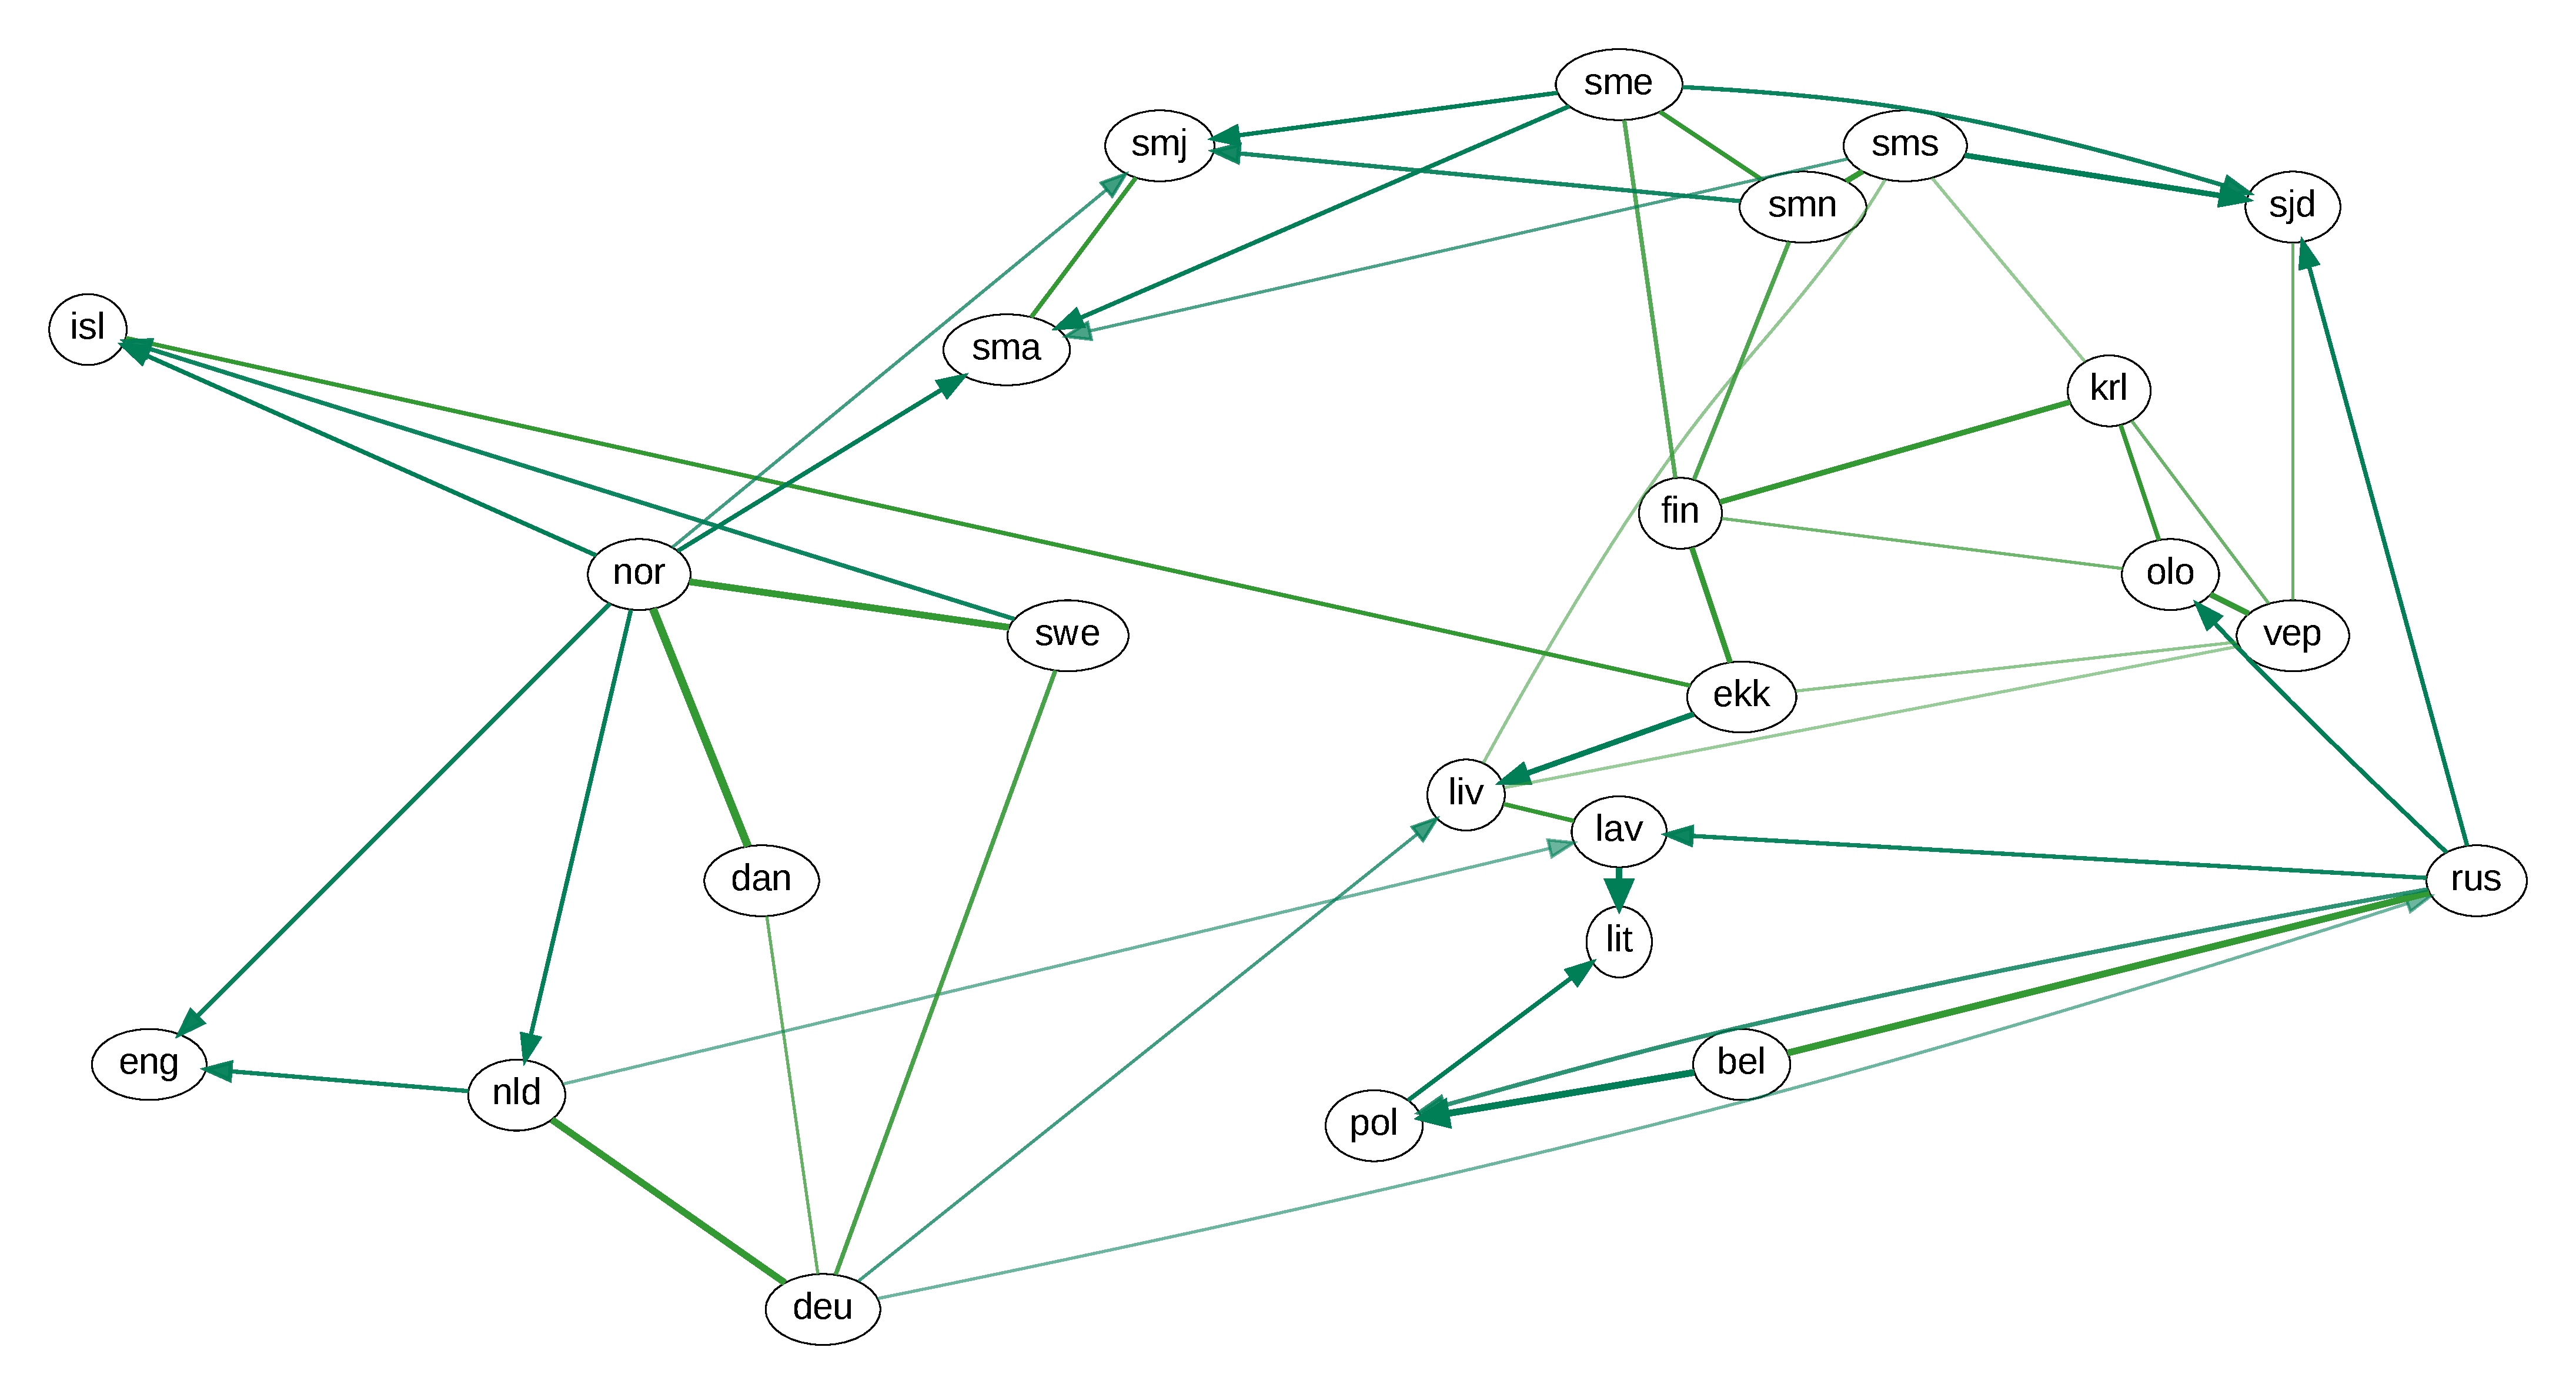
\includegraphics[width=\textwidth]{figures/baltic-contact-fs-tss.pdf}
 \vspace*{5mm}
 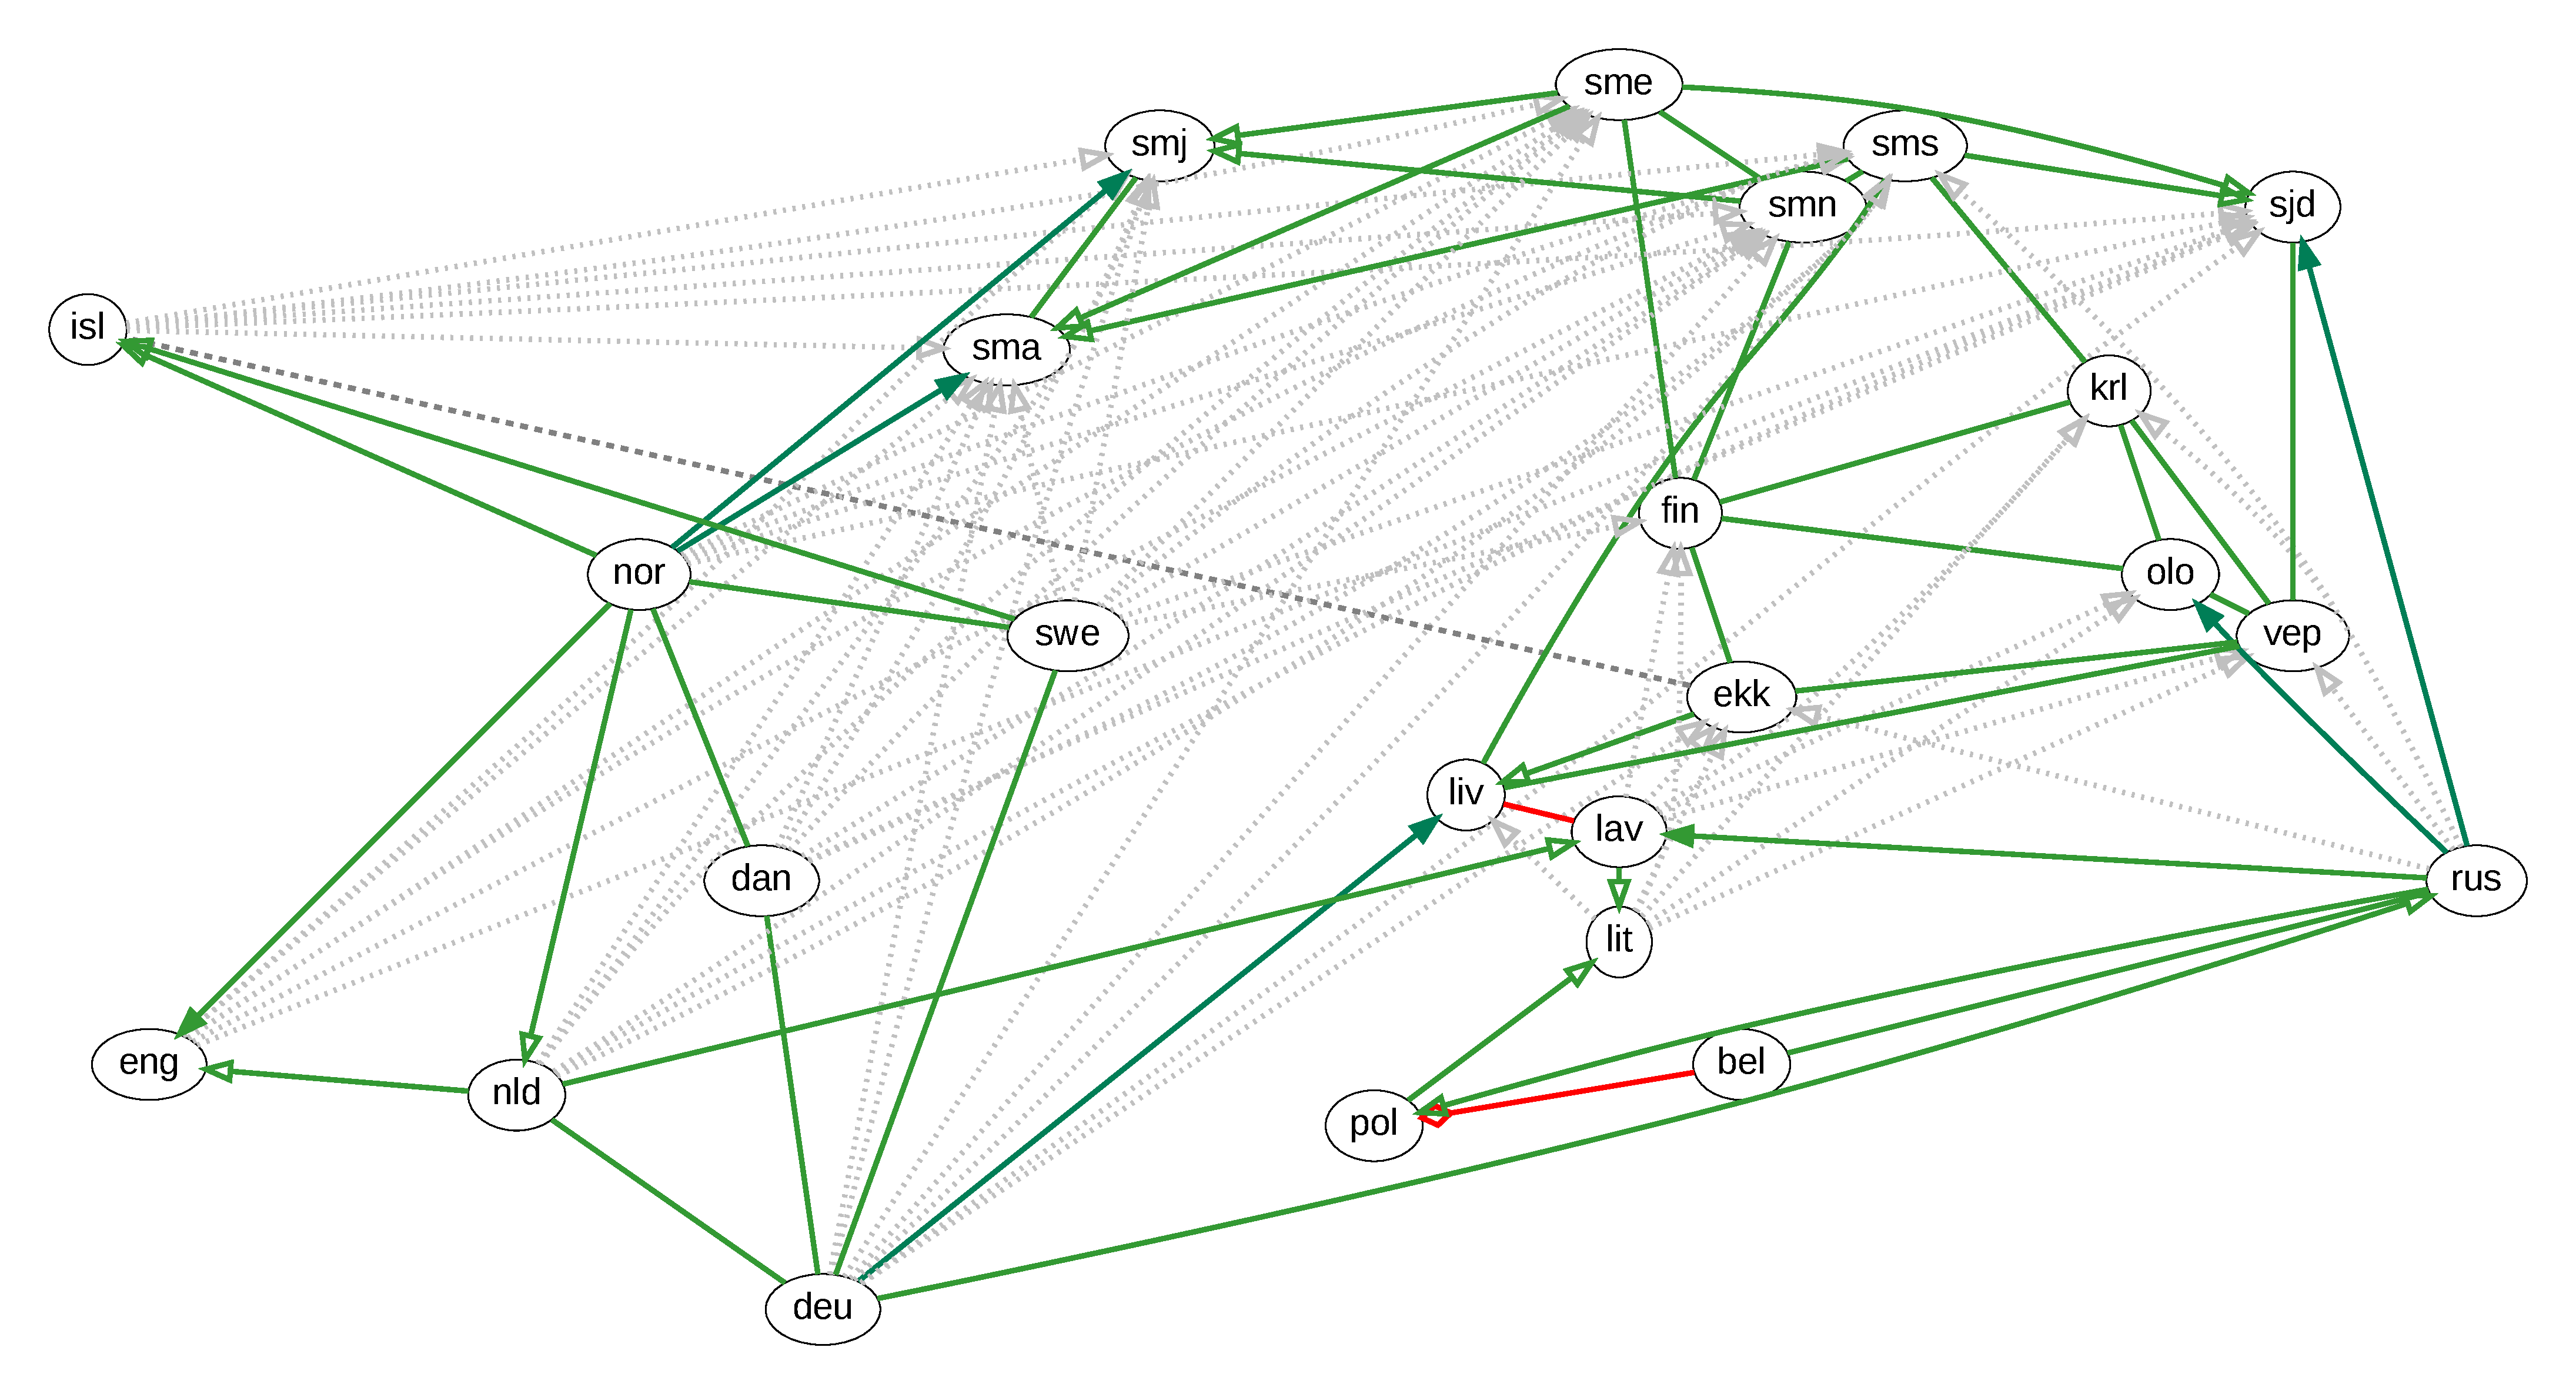
\includegraphics[width=\textwidth]{figures/baltic-contact-fs-tss-eval.pdf}
 \caption{Result and evaluation of contact flow on Baltic Sea data}
 \label{baltic-result-contact}
 \end{figure}
 
 \largerpage
 \subsubsection{Case study 2: Uralic and contact languages}
 \begin{sidewaysfigure}
 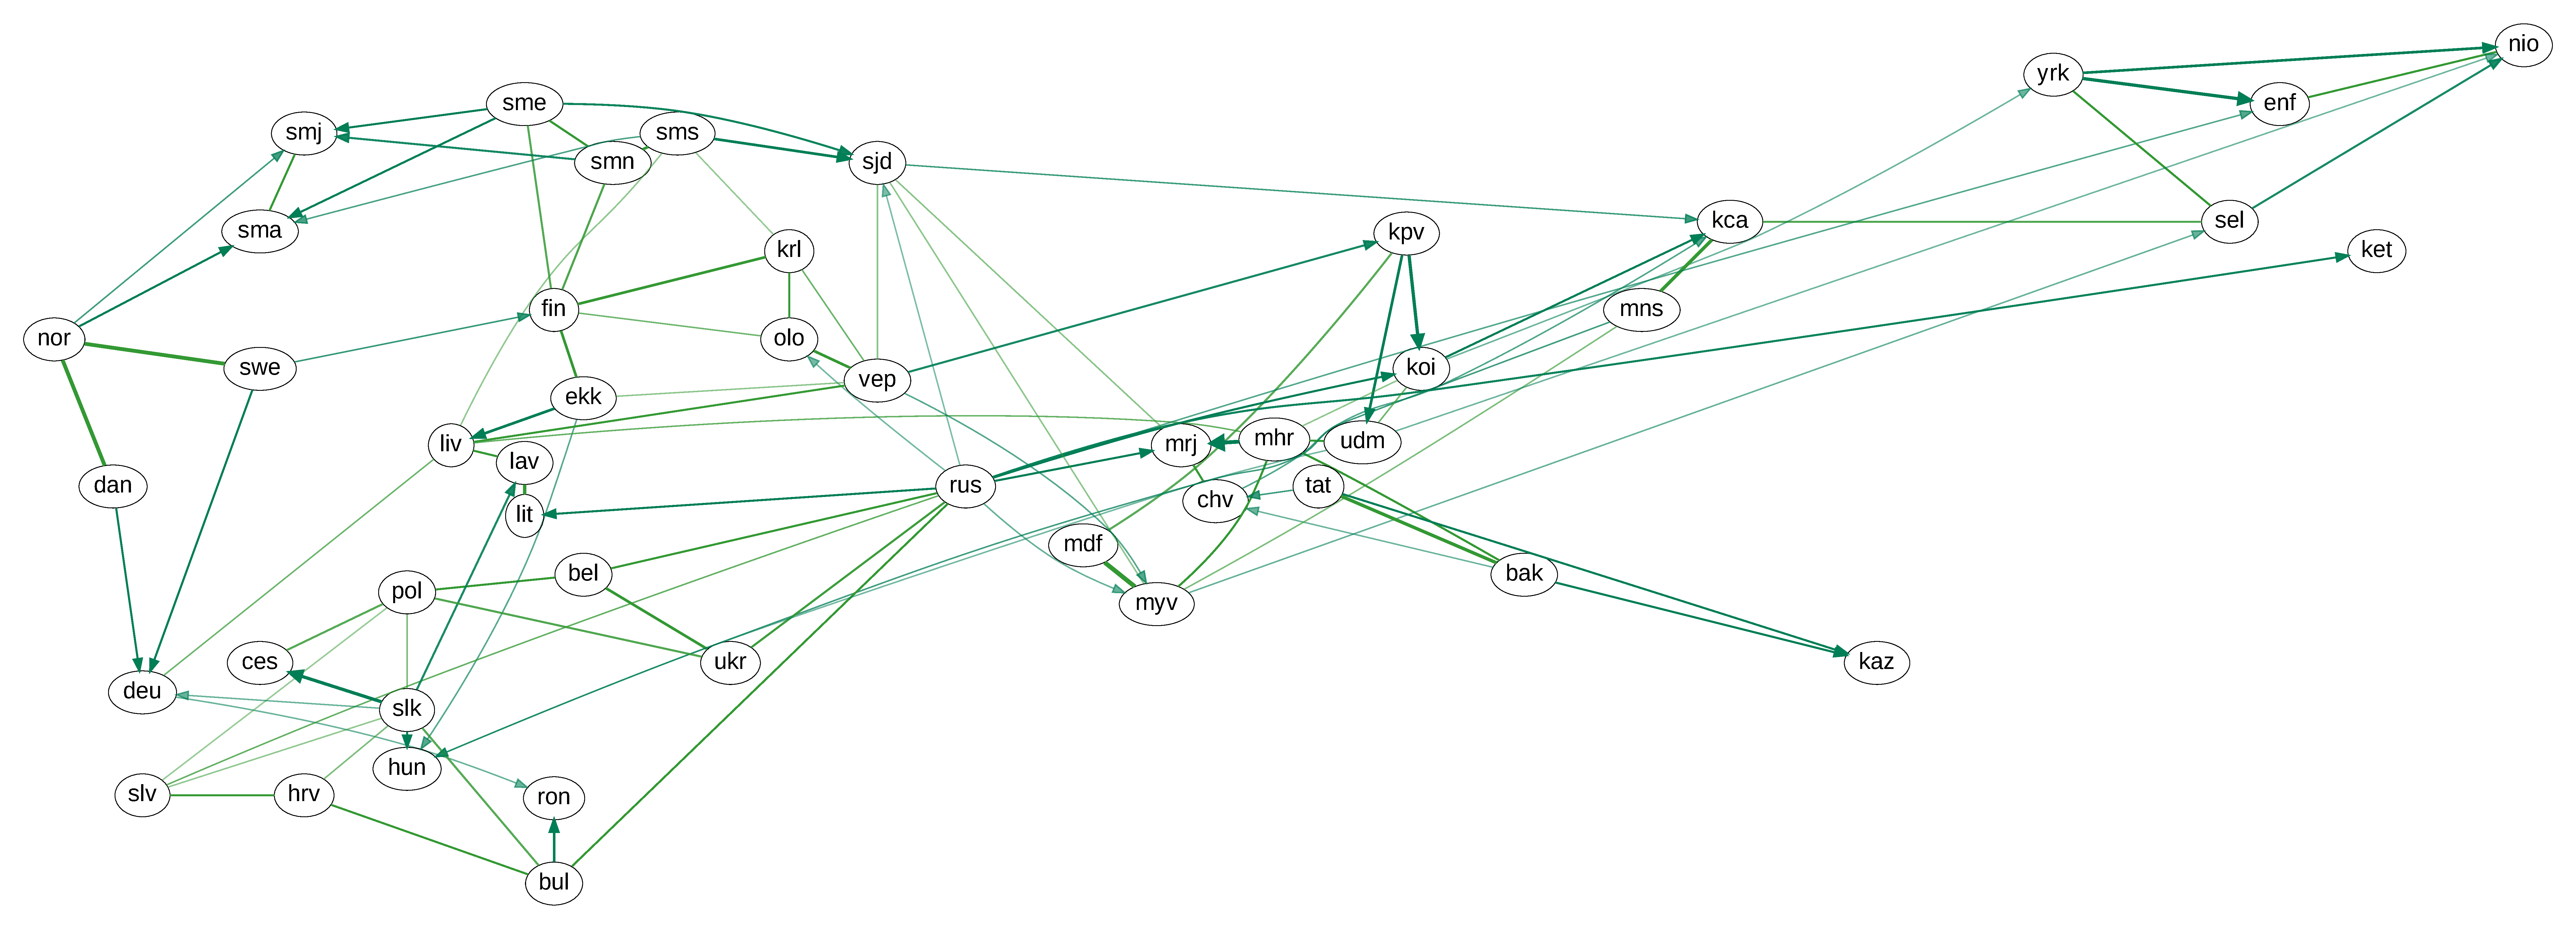
\includegraphics[width=\textwidth]{figures/uralic-contact-fs-tss.pdf}
 \vspace*{5mm}
 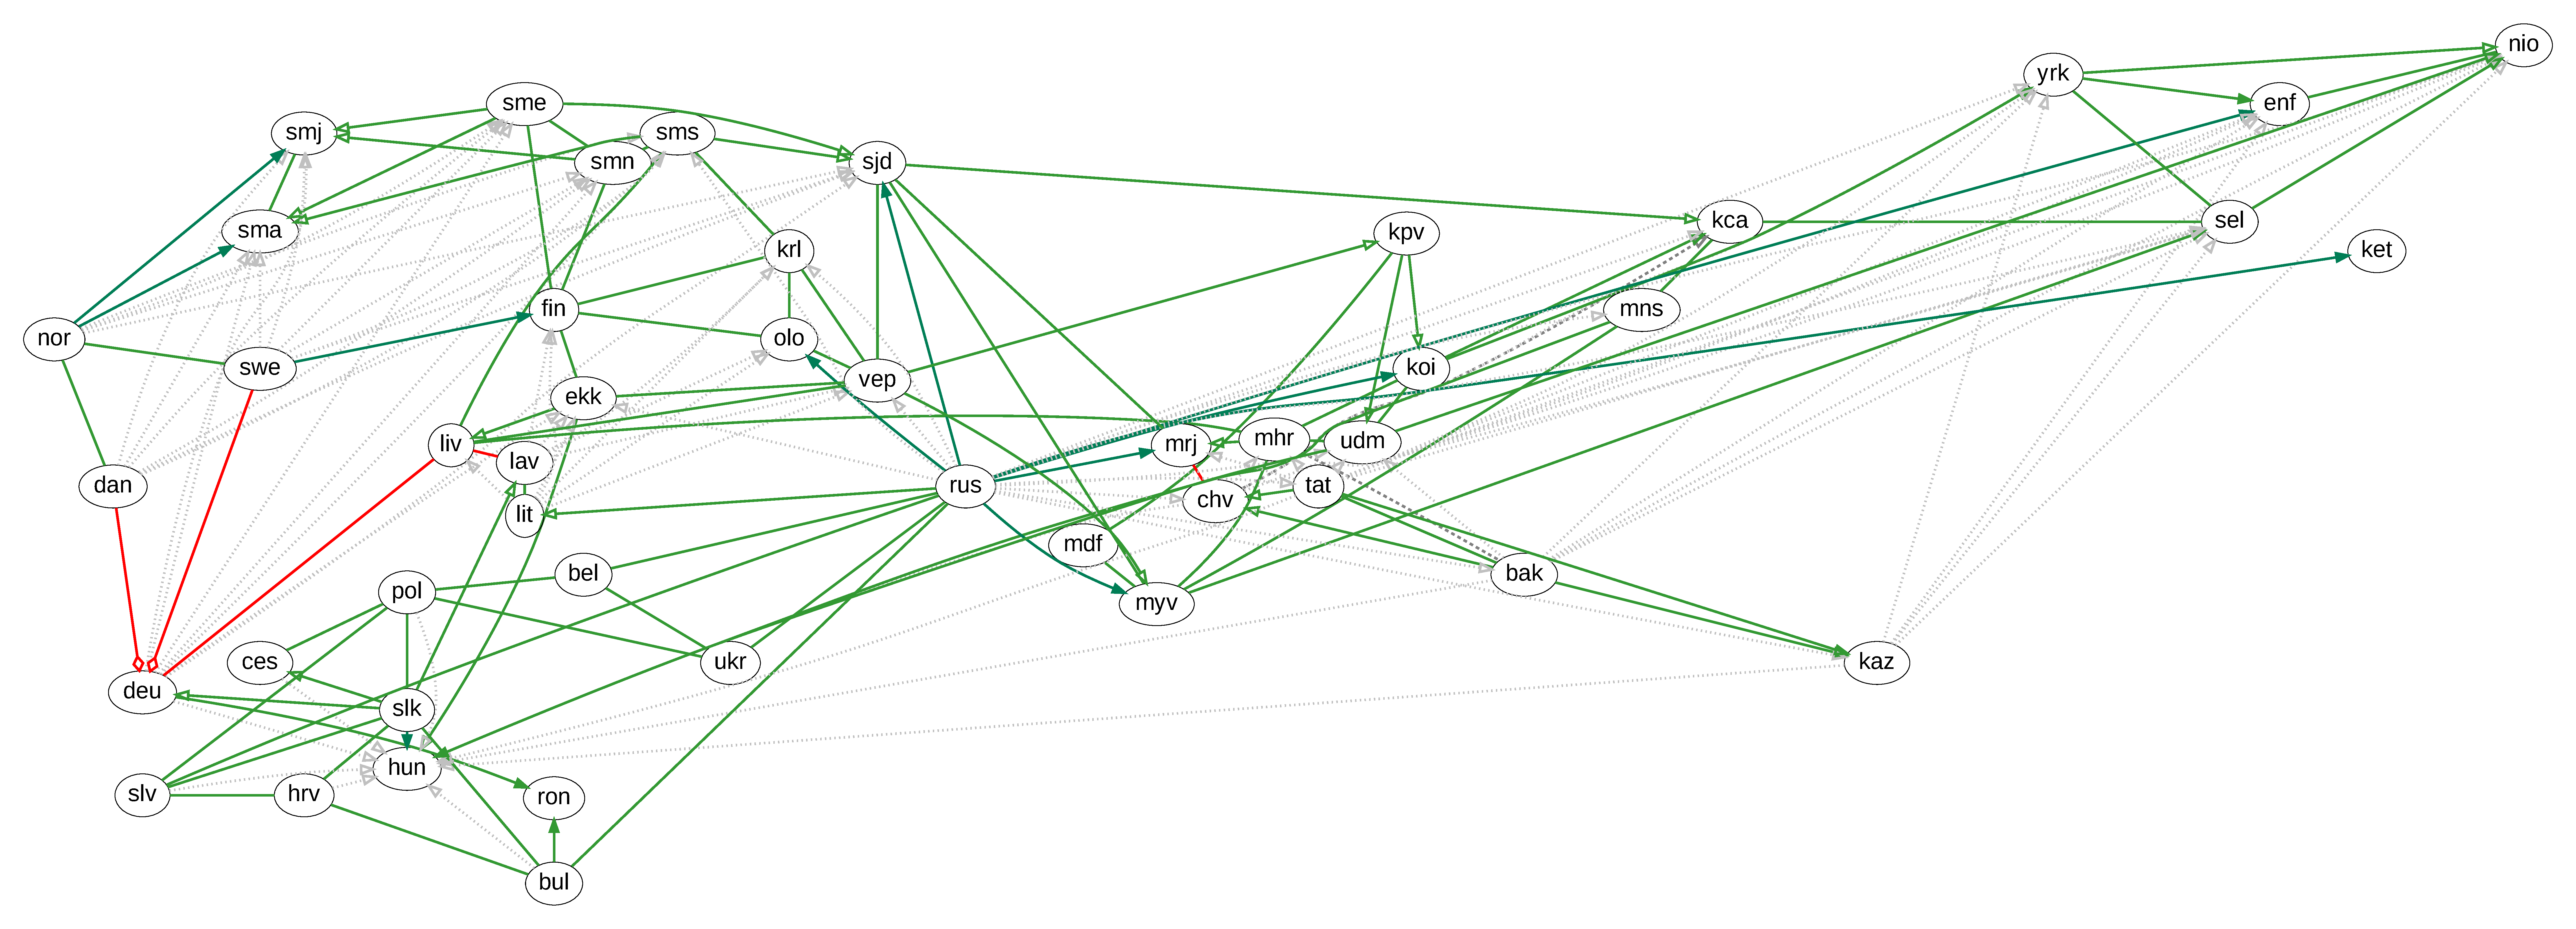
\includegraphics[width=\textwidth]{figures/uralic-contact-fs-tss-eval.pdf}
 \caption{Result and evaluation of contact flow on Uralic data}
 \label{uralic-result-contact}
 \end{sidewaysfigure}
 
The overall results of the Uralic case study, visualized in Figure \ref{uralic-result-contact}, are again quite convincing, especially in terms of phylum separation, with the exception of \ili{Kazakh} ($kaz$), which becomes separated from the other \ili{Turkic languages} by erroneous incoming directed arcs, and the wrong bidirected link between Latvian and Livonian, both of which were already explained in the first case study.
 
The only major problem with this result is a very interesting cluster of inverted arrows into \ili{German}, which did not appear in the smaller Baltic scenario, although it included all the involved languages as well. For \ili{Danish} and German, the triangles with \ili{Swedish} and \ili{Norwegian} are the only two relevant ones, and the same holds for Norwegian and Danish in reversed roles. The problem now is that all triples fit the v-structure assumption very well. For instance, for $dan \arrowLL deu \arrowLL nor$ we have a predicted overlap of 471 cognates according to the formula I derived, at an observed overlap of 482. The counterevidence scores for all triangles are below 0.1, i.e. they all fit the v-structure assumption very well. The problem is that the scenarios with German at the center tend to fit the v-structure assumption slightly better, so that we have a small amount of evidence against $deu \arrowLA dan$. The TSS score definition only builds on the ratio of scores, not on the actual strength of evidence, which leads to a TSS score ratio of 1.8 in favor of $dan \arrowLA deu$. In the Baltic sea scenario, this did not happen because \ili{Dutch} and \ili{English} provided further sources of high-overlap triples counterbalancing this difference. In general, having more languages in the dataset will always increase the stability of TSS, because there are more weighty triples to factor in. The fewer high-weight triangles are available for a language pair, the more unstable the TSS decision will be. We are going to see this effect very strongly in the Siberian case study.

Apart from this cluster of inverted arrows, the inferred contact flow network does not have any serious problems. The empty green arrows in the evaluation graph might serve to highlight a general difficulty of contact flow inference, however. To explain why so much spurious family-internal directionality is inferred, let us consider the \ili{Saami languages}. Like the other \ili{Western Saami languages}, \ili{Northern Saami} ($sme$) has loans from \ili{Norwegian}, but virtually all of these also exist in the smaller Saami languages that have been in even closer contact with Scandinavian languages. This means that it is most parsimonious for the model to explain away the connection from $sme$ to $nor$ by conditioning on $sma$ and $smj$. Locally, this causes the two languages to look like mixtures of their more easterly relatives with Norwegian, leading to directional arrows from $sme$ and $smn$ into $sma$ and $smj$.

\subsubsection{Case study 3: the linguistic landscape of Siberia}
 
\begin{sidewaysfigure}
 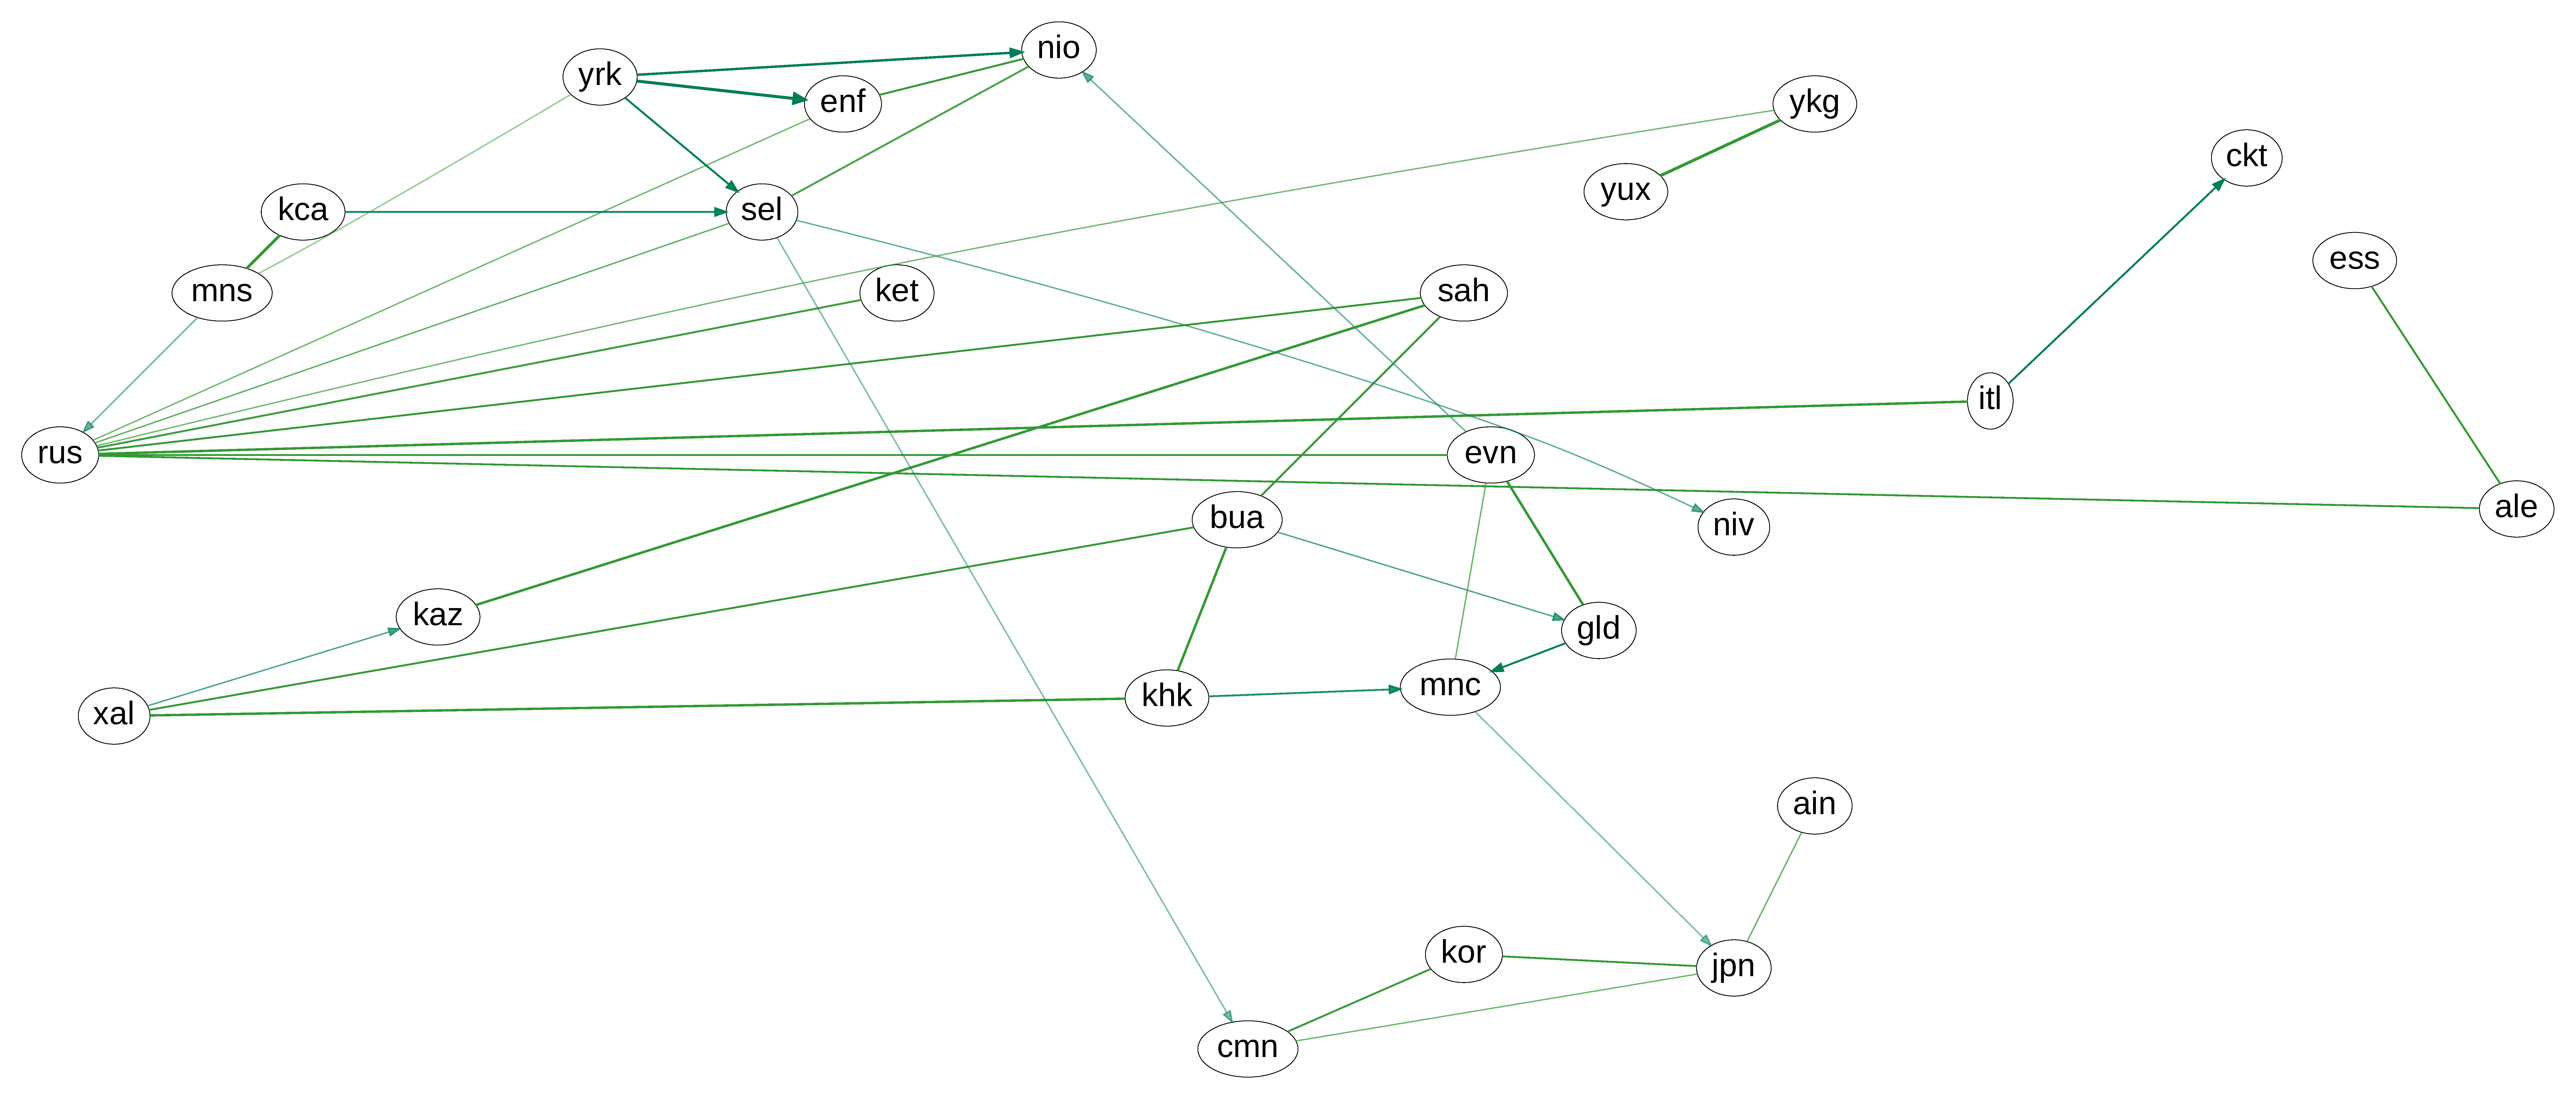
\includegraphics[width=0.8\textwidth]{figures/siberia-contact-fs-tss.pdf}
 \vspace*{5mm}
 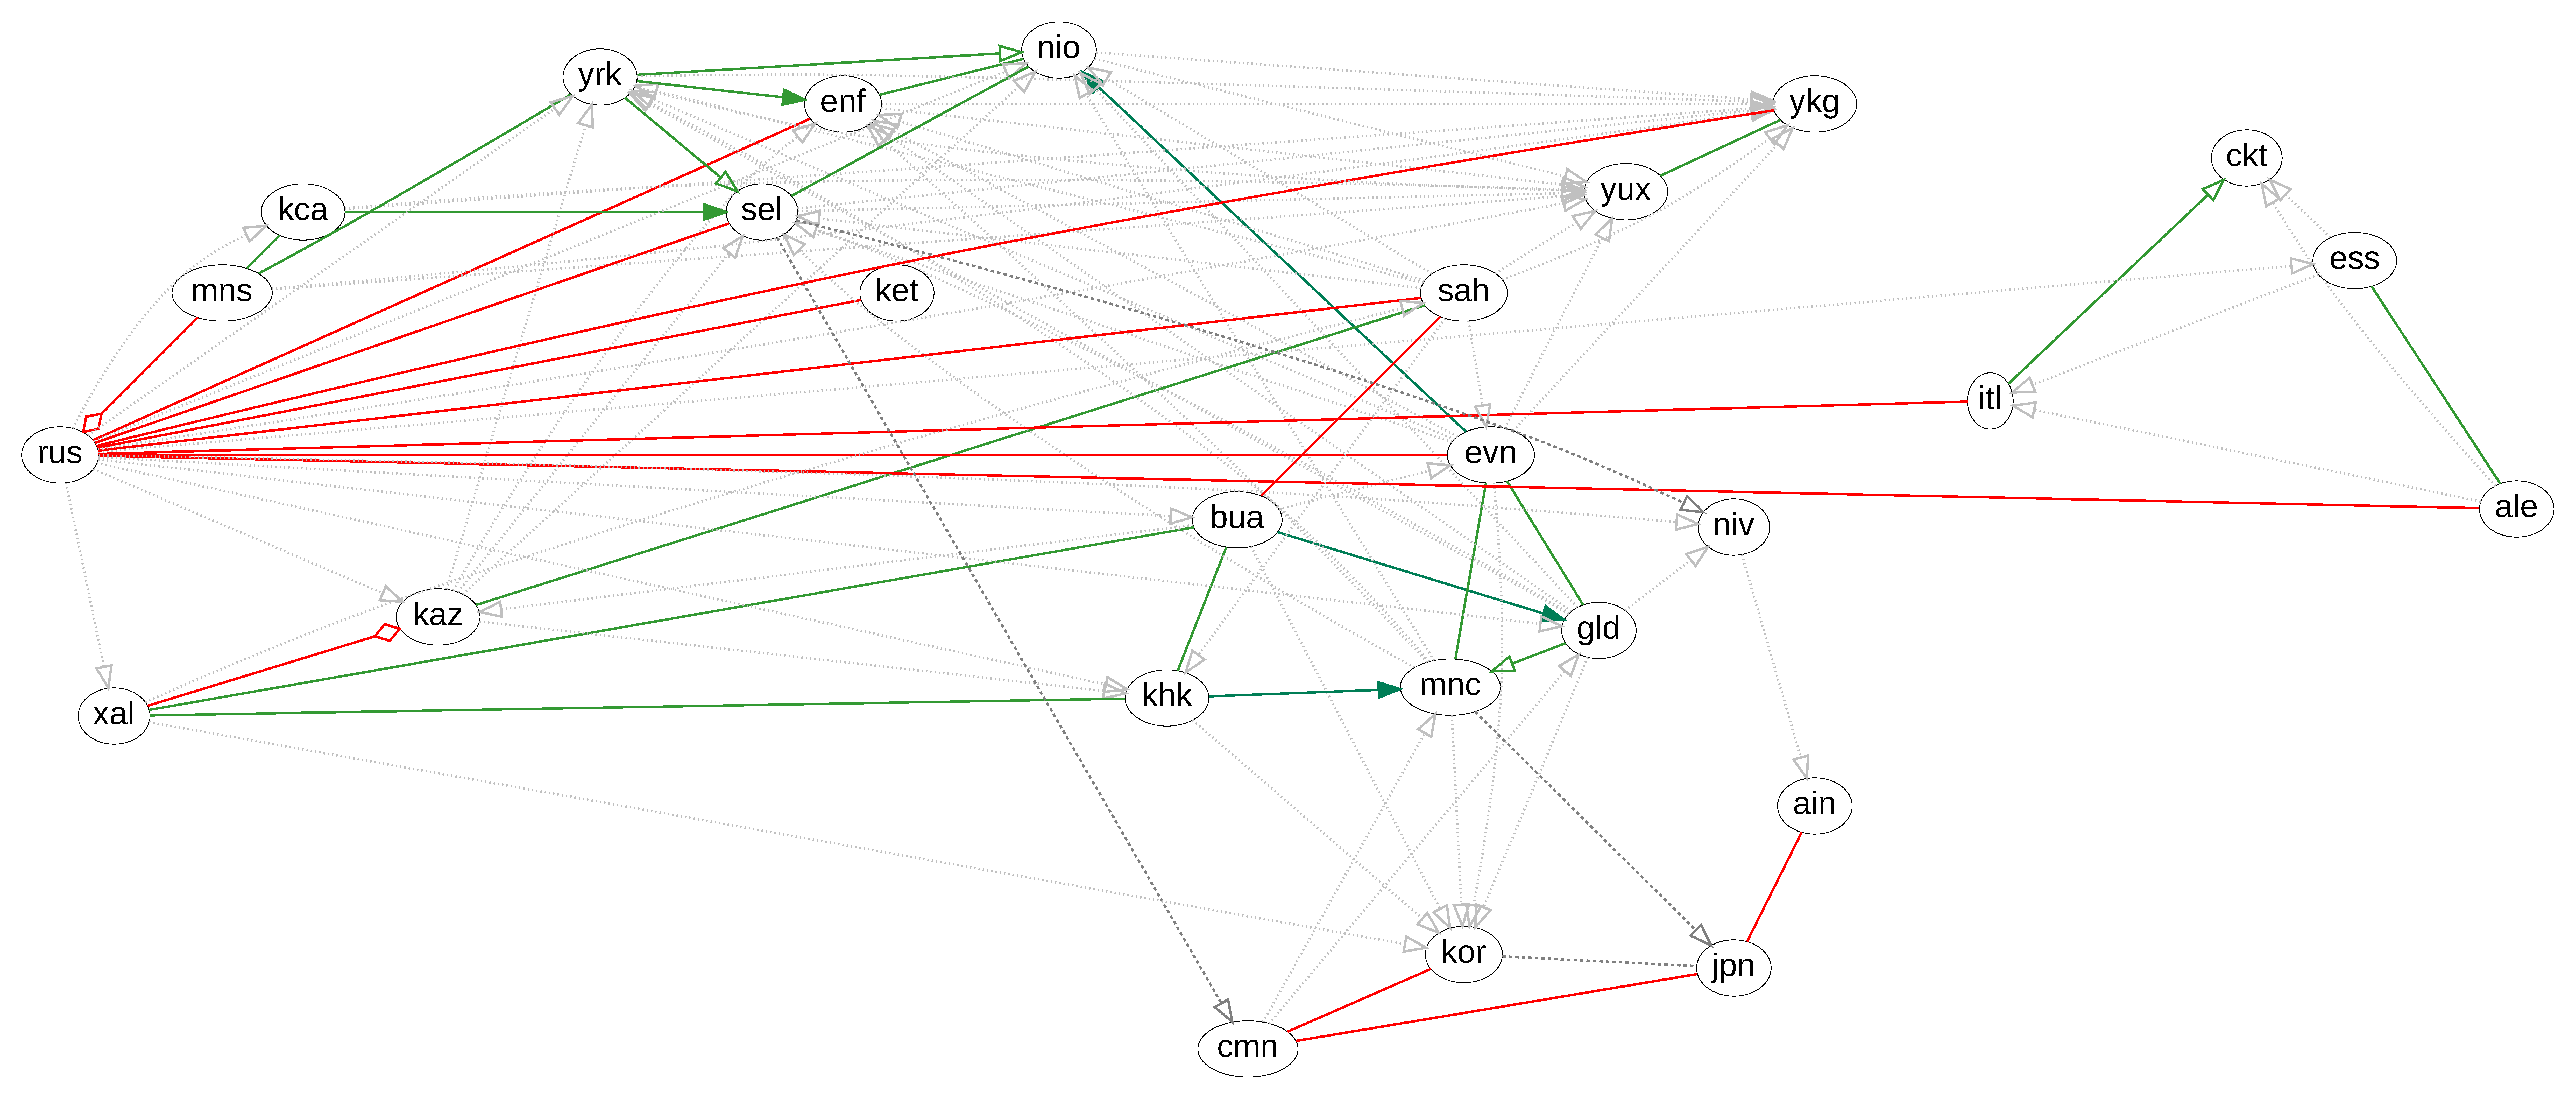
\includegraphics[width=0.8\textwidth]{figures/siberia-contact-fs-tss-eval.pdf}
 \caption{Result and evaluation of contact flow on Siberian data}
 \label{siberia-result-contact}
\end{sidewaysfigure}
 
 In this scenario, the results of CLFI are actually worse than those of PLFI. As the results in Figure \ref{siberia-result-contact} show, the star-shaped influence of \ili{Russian} on various minority languages is not recognized any more, in most cases leading to bidirectional arcs. This is again due to a lack of high-overlap triples involving the links in question. In the global NorthEuraLex network, the star pattern was inferred just as intended, because there were other \ili{Slavic languages} in the dataset which could serve to form high-overlap triples involving Russian. To see even more clearly how this problem is ingrained in the mechanics of TSS computation, let us take a look at some details behind the pair $rus \arrowLL sah$. The following third languages contribute the most to the triangle score sum: \ili{Kazakh} (30.3\%), \ili{Itelmen} (12\%), \ili{Buryat} and \ili{Kalmyk} (at 6.7\% each). We only have $|cog(rus,sah,kaz)| = 7$, against an overlap of 3.74 predicted for $rus \arrowLA sah \arrowAL 
kaz$, and 13.36 for $sah \arrowLA rus \arrowAL kaz$. The fit of both predictions with the true overlap is thus about equal. This pattern repeats for the other triangles, so that the score ratio reaches only 1.029, a signal which is weaker than any reasonable threshold. For other minority languages, the pattern repeats itself, even if some pairs like $rus \arrowLA ykg$ (TSS ratio 1.357) are much closer to the threshold. So why did everything work much better in the larger scenarios? The reason is that any additional Slavic language such as \ili{Ukrainian} will provide a high-overlap unshielded triple $ukr \arrowLL rus \arrowLL sah$, because Russian will screen off the Russian minority languages from $ukr$ during skeleton inference. The TSS criterion yields very high evidence against this being a v-structure, which tips the balance in favor of arrows going out of Russian for all languages Russian separates from Ukrainian. To summarize, TSS helps to aggregate and weight evidence from different triples, but in 
the absence of unshielded triples creating strong directional signals, TSS will be unstable or inconclusive. Using a pairwise score like TSS does not provide a means to overcome the theoretical results about causal inference, which tell us that unshielded triples are needed to securely establish the direction of causality.
 
 A further interesting phenomenon is displayed by the two-member Chukotko-Kamchatkan\il{Chukotko-Kamchatkan languages} family. \ili{Itelmen} ($itl$), the language whose lexicon was influenced much more strongly by Russian, is inferred to have been the intermediary for transmitting the Russian loans into \ili{Chukchi} ($ckt$), yielding a directional signal between the two related languages. This is a problem that is especially virulent in small language families, which is why we have not yet seen it in the other case studies. The wrong internal structure of Tungusic\il{Tungusic languages} is also created by $evn$ as the obvious entry point for all the Russian loans, which then get transmitted within the family on the path $evn \arrowLA gld \arrowLA mnc$, although this effect is not strong enough to yield a directional signal above the threshold.
 
 Finally, failure to recognize the directionality of contacts between \ili{Chinese}, \ili{Japanese}, and \ili{Korean} is again due to the absence of high-overlap triples that would yield directional information. The most relevant triple for all connections between these three isolates (in our study) is the one formed by the three languages. But the three-way overlap between the three languages is only very small at $|cog(cmn,jpn,kor)| = 14$, showing that the expected problems with recognizing Chinese loans based on \ili{Mandarin Chinese} have indeed materialized. In this triangle, there is not enough room for different directions to vastly differ in the fit of their prediction to the true overlap size, leading to hints of equal strength in every direction. In general, lexical flow inference will always run into problems when isolates are involved, and we can only expect it to work well if both languages connected by the link of interest have close relatives in the dataset. This is the reason why contact flow 
inference worked so much better on the Baltic Sea and Uralic test sets (where larger families meet) than in isolate-ridden Siberia, where even the colonial language is an isolate in our dataset.
 
 \subsubsection{Case study 4: a visit to the Caucasus}
 \begin{figure}
 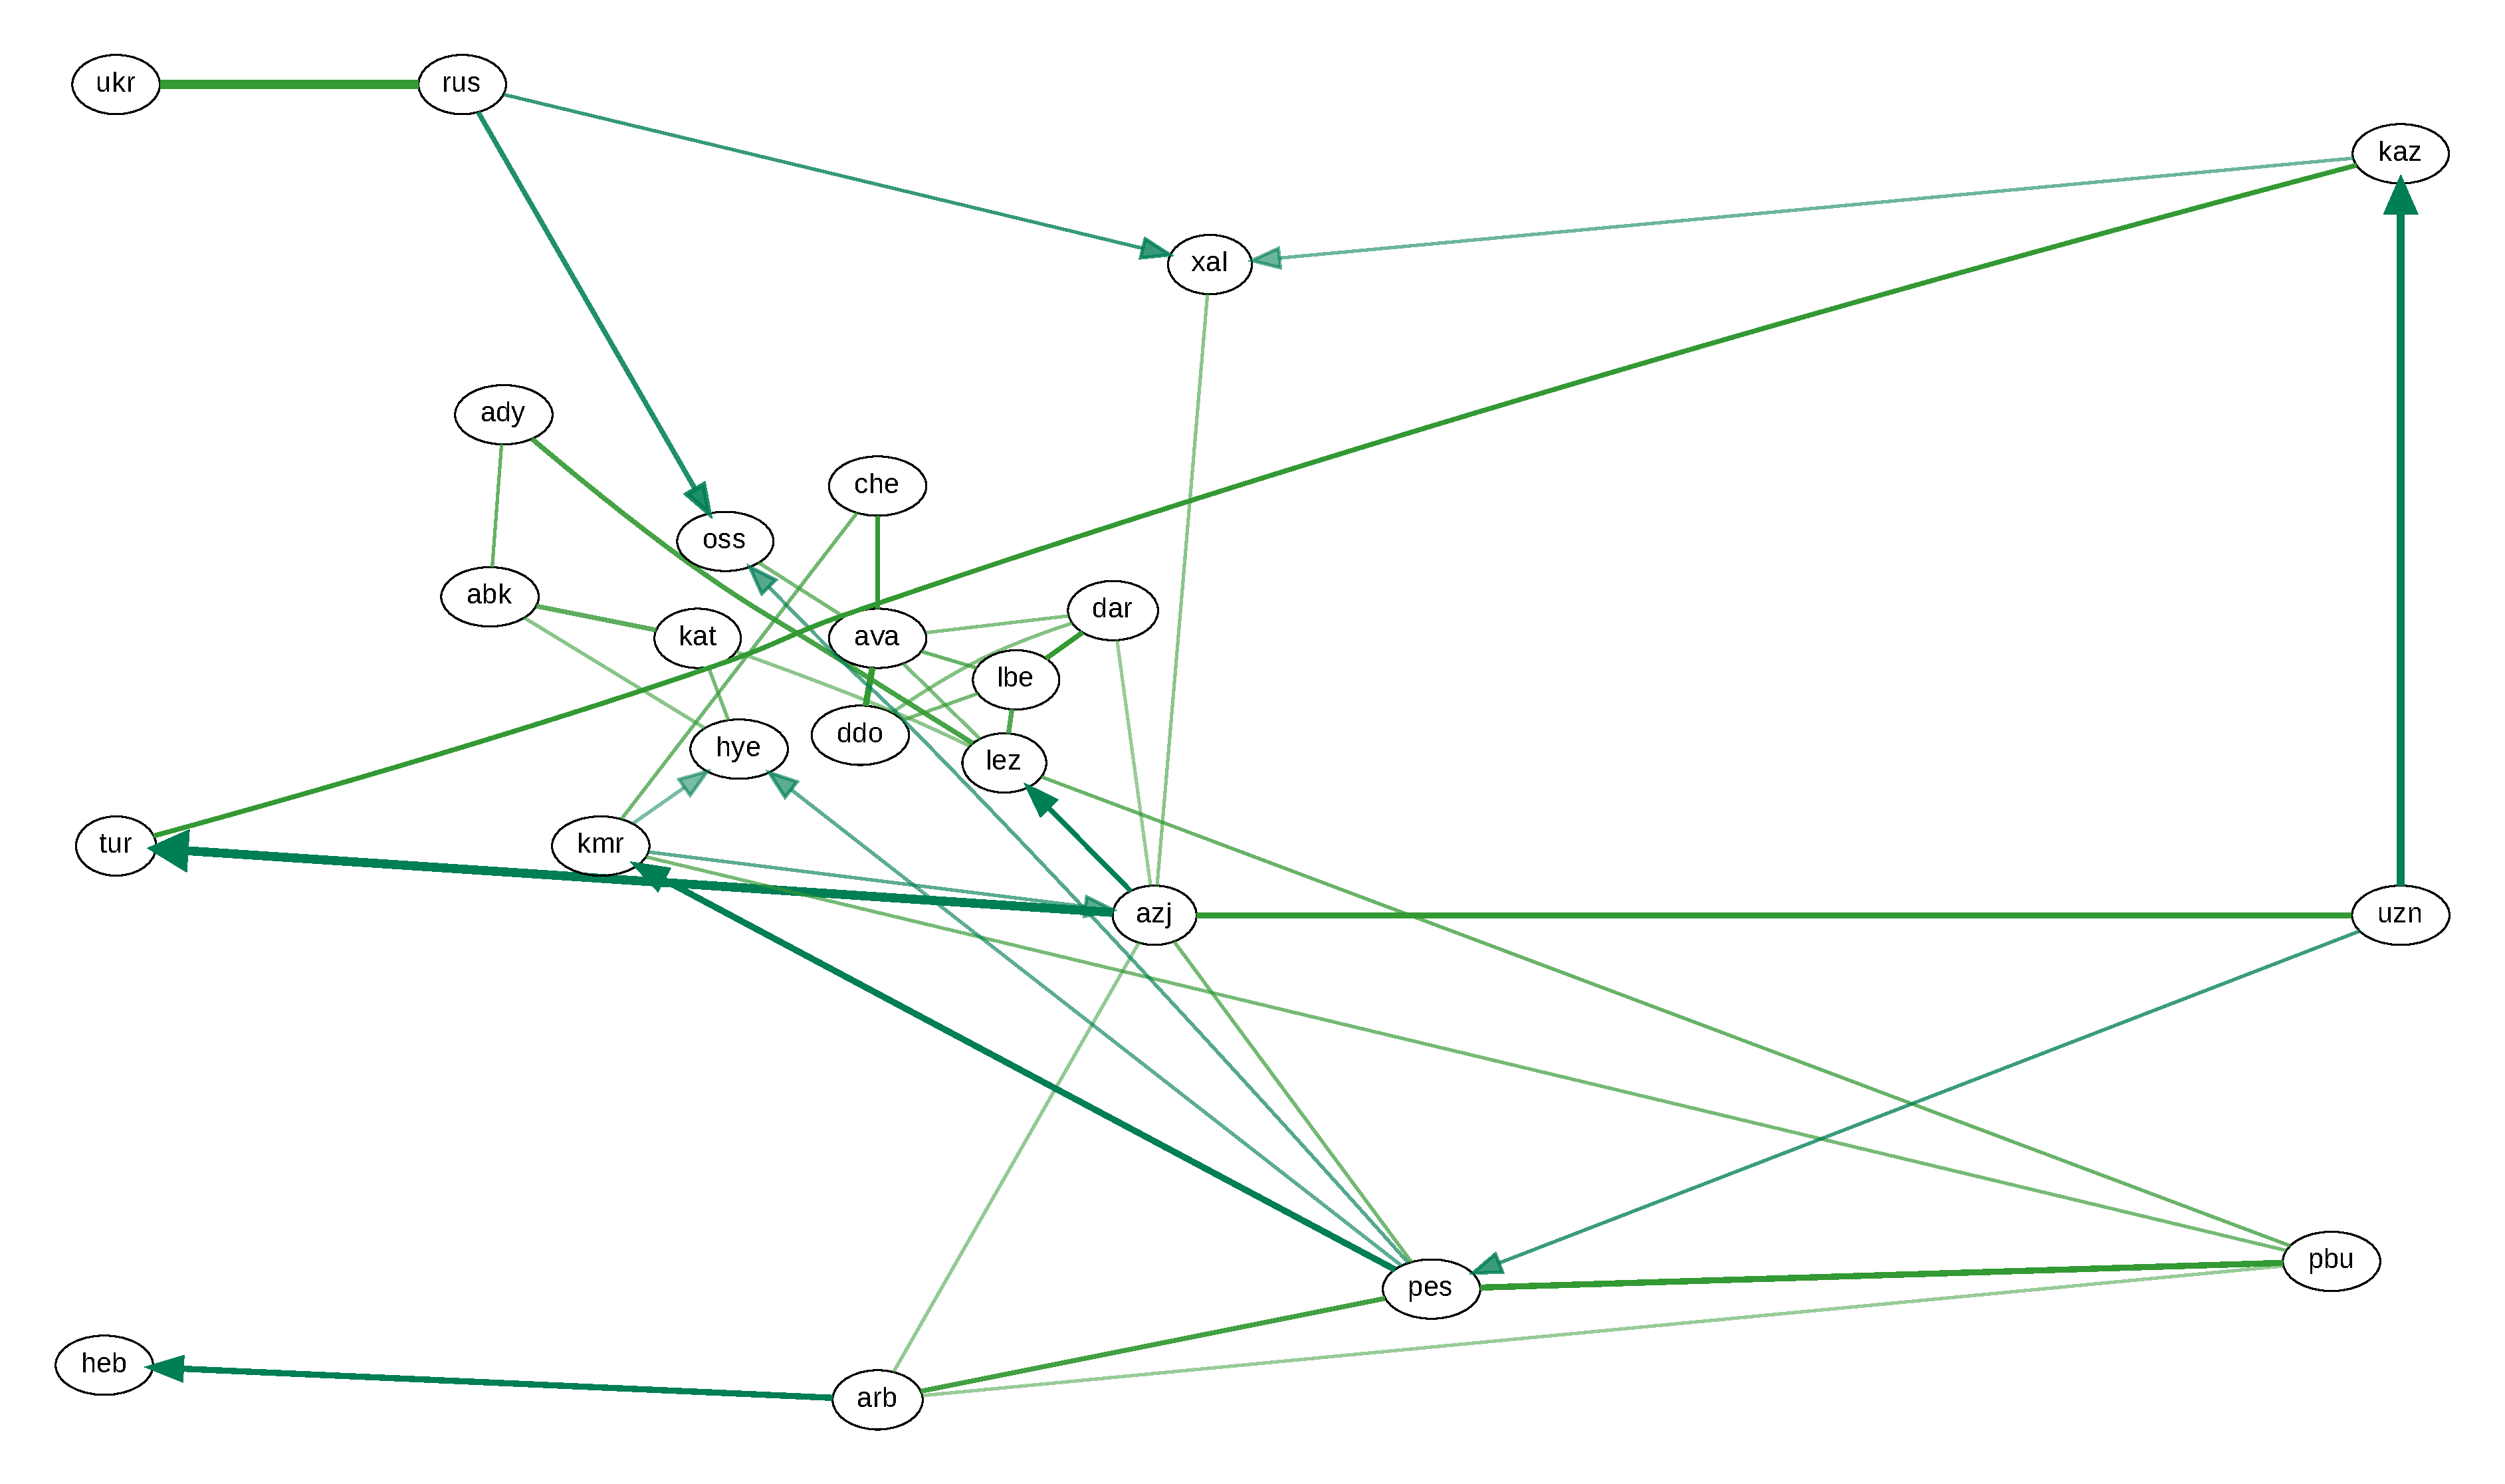
\includegraphics[width=\textwidth]{figures/caucasus-contact-fs-tss.pdf}
 \vspace*{5mm}
 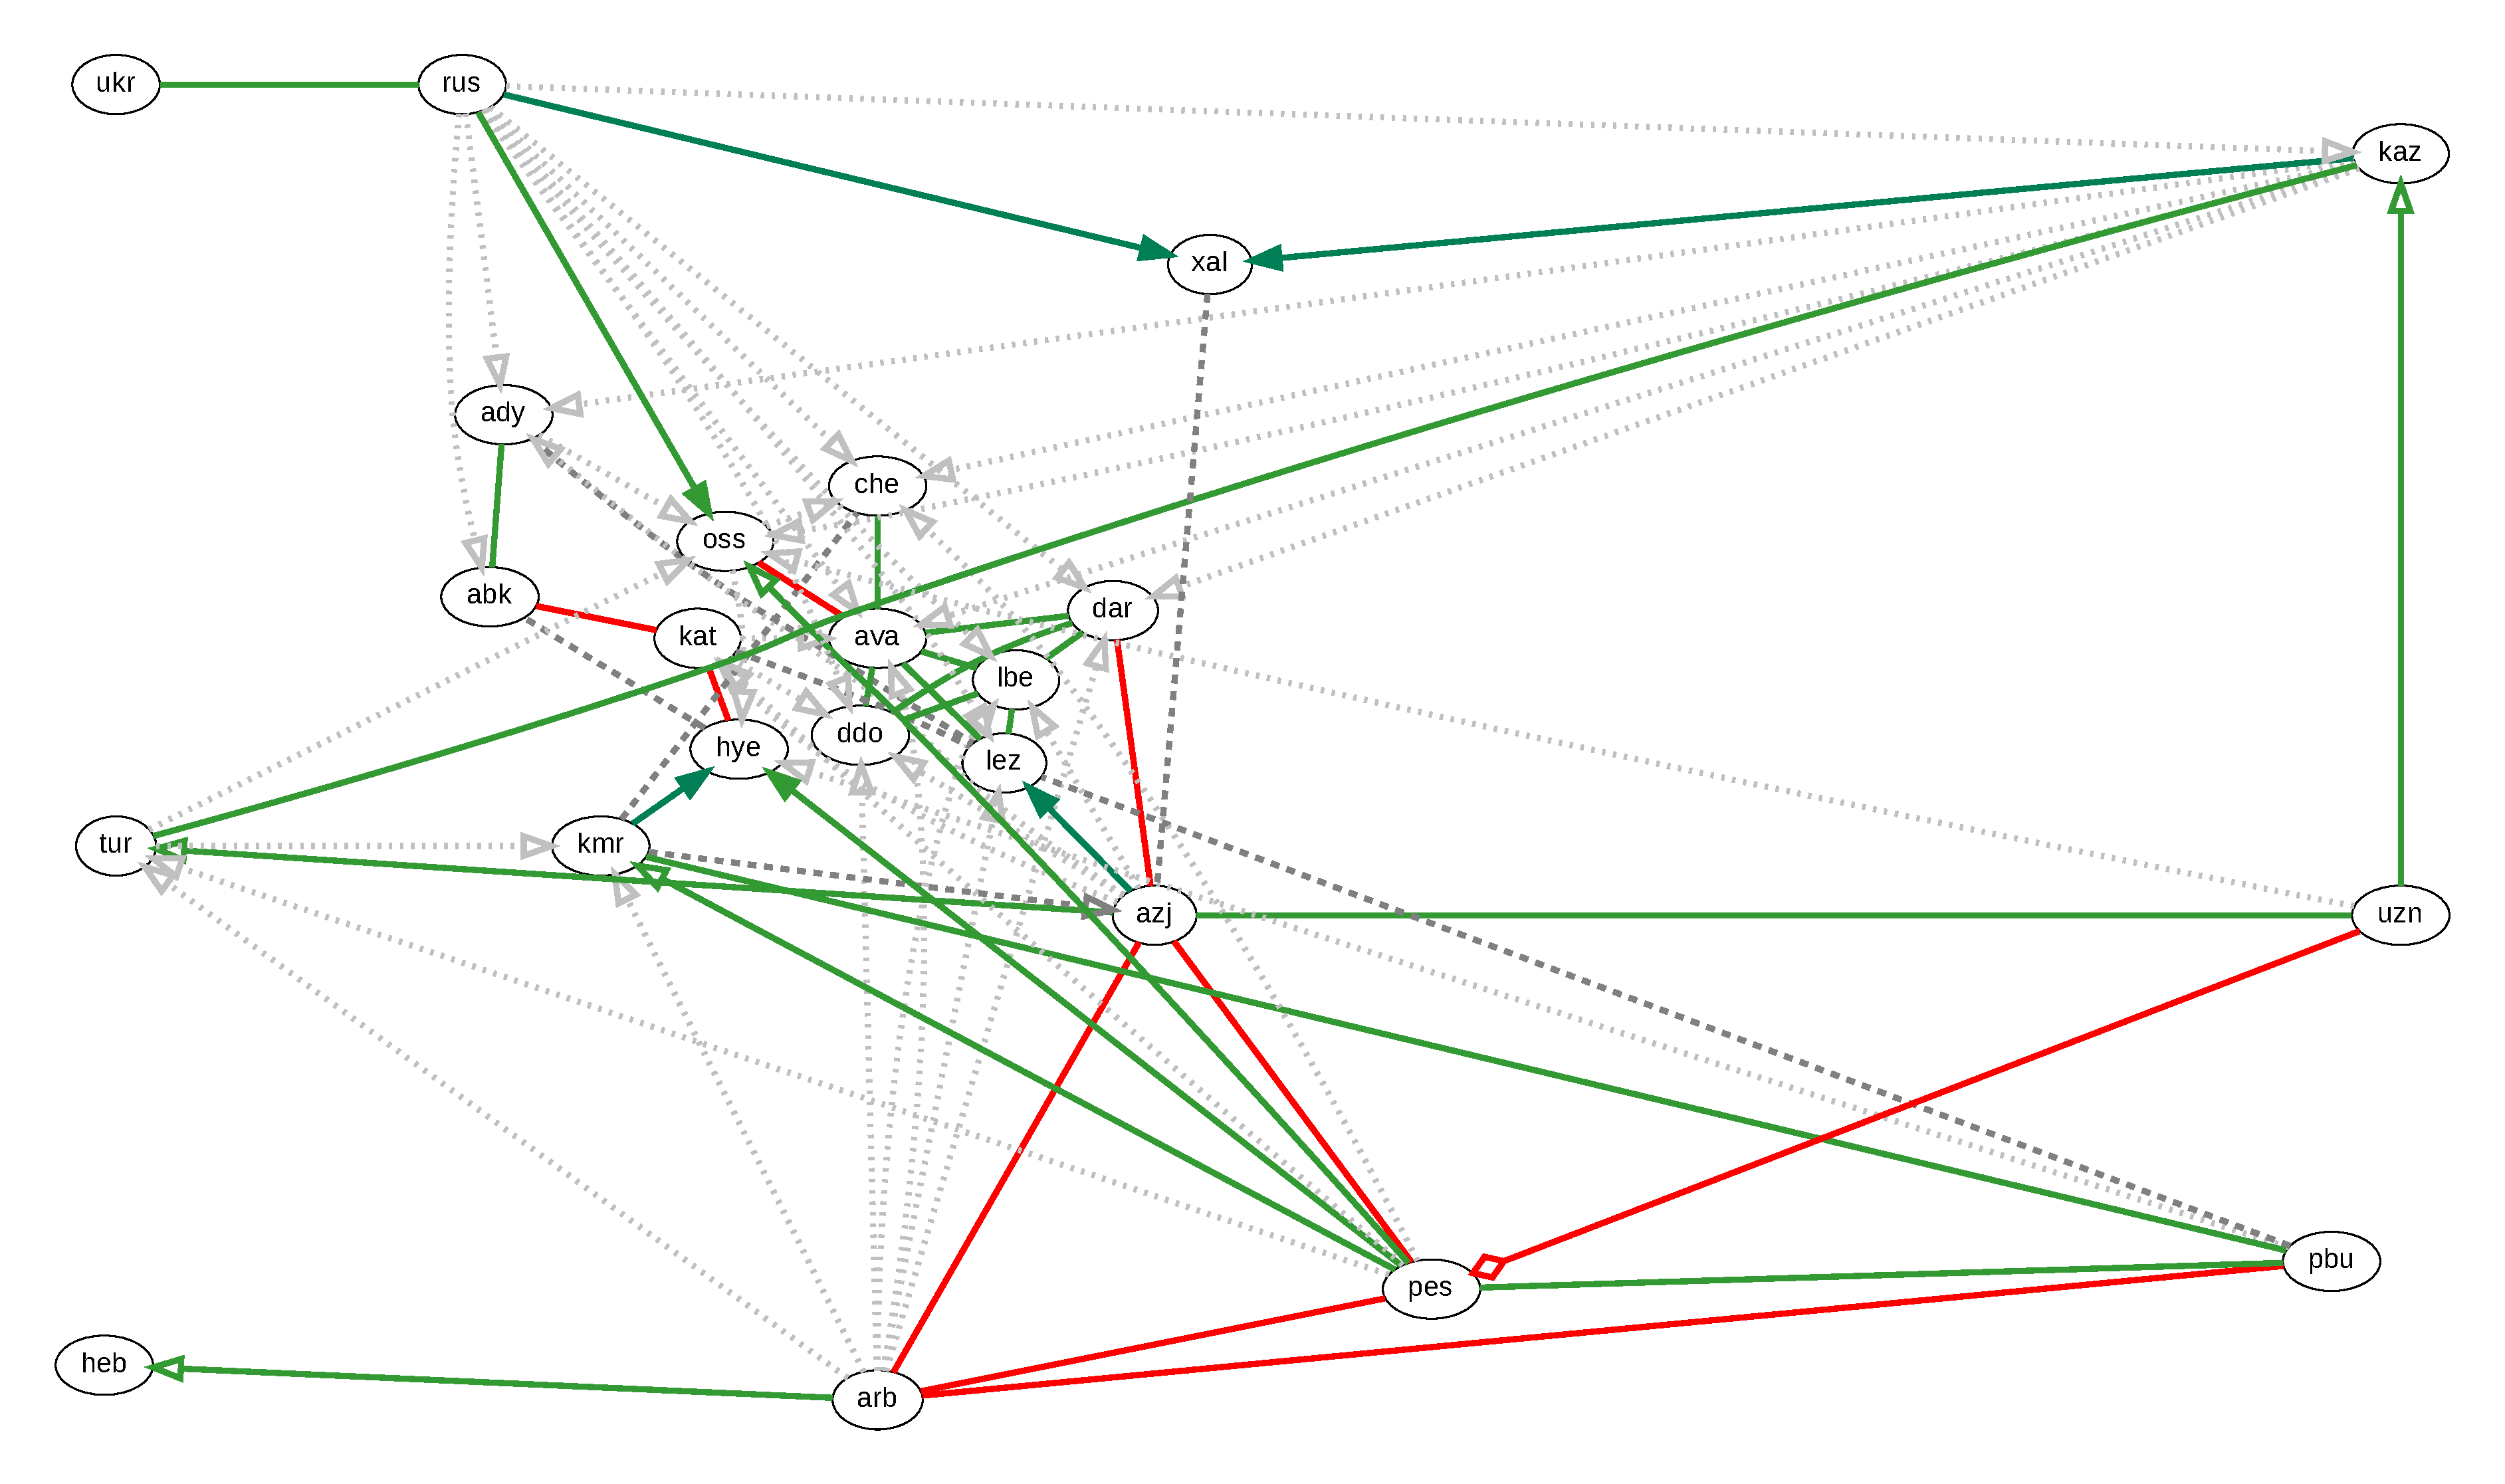
\includegraphics[width=\textwidth]{figures/caucasus-contact-fs-tss-eval.pdf}
 \caption{Result and evaluation of contact flow on Caucasian data}
 \label{caucasus-result-contact}
 \end{figure}
 
 In the results of the Caucasian case study visualized in Figure \ref{caucasus-result-contact}, it turns out that the absence of a proto-language does not help us prevent the erroneous arrow from \ili{Uzbek} into \ili{Persian}. The reason is that all the triangles formed from two Turkic languages plus Persian look very much like v-structures according to the predicted overlaps. This is not an issue of data sparseness as in previous cases, because the three-way overlap for such triples will typically exceed 60 cognates. Instead, the problem now is the very high overlap between the \ili{Turkic languages}, which would lead to a three-way overlap of the predicted size even if the true story were a v-structure. This is an instance of one of the cases where the TSS criterion is inadequate.
 
 The second interesting question in this case study is why \ili{Arabic}, which was correctly established to be a major external source of lexical material for the region in UFR-based PLFI, is a source of problems for TSS-based CLFI. Again looking at the TSS score ratios first, we find that the main problem is the triple of \ili{Persian}, Arabic, and \ili{Pashto}, with an overlap of $|cog(arb,pes,pbu)| = 70$ which does not fit the story $arb \arrowLA pbu \arrowLA pes$. The problem here is the assumption of independent sampling. The Arabic loans in Persian and Pashto overlap a lot more than the assumption of independent contacts would suggest, because they are concentrated in the religious and scientific vocabulary. This non-collider signal counteracts the collider signals coming from triples such as $arb \arrowLL pes \arrowLL kmr$. To alleviate this type of problem, one would need a much more explicit flow model which would model the flow beyond the local configuration, enforcing the constraint that there must be a directed path between any pair of languages that share a substantial marker of cognates, and take this into consideration when making local directionality decisions. Unfortunately, it is highly unlikely that inference in such a flow model would be tractable at the scale at which I am operating.

\subsection{Evaluation on simulated data}
As the final part of this chapter, I again check whether we can reproduce our findings about the relative performance of different CLFI variants on the simulated data. This time, a little more thought than before must go into the definition of the gold standard. 

\subsubsection{True and detectable histories}
For NorthEuraLex, the inclusion of a contact link into the gold standard presupposed the existence of a discernable layer of loans in the attested part of the language. While this was sometimes difficult to assess based on the available literature, it still provided an external way of getting at the desired information, and the resulting evolutionary network was already relatively flat similar to a contact flow network, because ancient contacts are less clearly known, and less frequently discussed in general descriptions of individual languages.

The main issue in generating such gold standard graphs for the simulated scenarios can be conceptualized as the difference between true and detectable histories. The \textit{true history} is what actually happened during the simulation, including contacts with substrate languages, i.e.\ languages without living descendants about whose existence we can only know due to loanwords they left in attested languages. This makes the true history easy to define based on the simulation trace.

In contrast, the \textit{detectable history} is only a subset of the events contained in the true history, informally defined as containing all the events of which some trace is still visible in the cognate data for living languages. By means of the detailed protocol of the complete history for each simulated scenario, the visibility of each event can be determined exactly by checking whether it is part of any word trace leading to a cognacy relation in the input data.

\subsubsection{Summarizing generated contact histories}
A true history gold standard will simply contain every contact link through which more than 25 lexical items were transmitted (based on 1,000 simulated concepts, and our CMI threshold of 0.025). However, expecting CLFI to infer this true history will not lead to a fair assessment of the system's performance. Instead, we need a gold standard that is comparable in difficulty to the equivalent task on the NorthEuraLex data. In other words, we need a way to extract a picture of the history of the linguistic region from the simulation protocols that is roughly comparable in shape and abstraction level to the NorthEuraLex gold standard.

This leads me to the following solution for generating gold standard graphs for the simulated data: Exploiting the existing infrastructure for tracing the history of every attested word (the detectable history), we consider each pair of languages in turn, and count the number of current words that were once borrowed from one language or one of its ancestors to the other language or one of its ancestors, stopping once we meet the lowest common ancestor of both languages. After discarding borrowing events which took place within the same cognate class, we arrive at a total number of transferred items in both directions, and put the appropriate arrow into the gold standard network if the number of borrowings in the respective direction exceeds 10 lexical items.

\subsubsection{Results}
Again, we start with the skeleton performance data in \tabref{contact-skeleton-evaluation-simulated}. The skeleton recall numbers are globally much better than on the NorthEuraLex data, and the differences between the different separation methods are again rather small, especially the difference between PC and FCI skeletons. Since the simulated gold standards based on detectable histories are defined in a much more objective way than the NorthEuraLex gold standard, the difference in recall suggests that a large portion of the contacts postulated by the NorthEuraLex data might not actually be detectable from the data, and that quite a few links, especially those reflecting very ancient contacts, should be removed from the gold standard. Apart from this difference, the small divergences in performance between skeleton inference methods show a very similar pattern as on the NorthEuraLex data, although this time, FCI consistently performs better than the vanilla PC algorithm. This difference once more illustrates that FCI can only play out its strengths on very clean datasets such as my simulated data, whereas it appears very prone to be affected by the type of noise seen in automatically inferred cognacy overlap data.

\begin{table}
 \centering
 \begin{tabular}{ccccc}
 \hline \hline
   & \multicolumn{2}{l}{Overlap separation} & \multicolumn{2}{l}{Flow separation}\\ 
   & VPC & FCI & VPC & FCI\\ 
 \hline
  skPrc & \textbf{0.966} & 0.963 & 0.933 & 0.934\\
  skRec & 0.559 & 0.621 & 0.740 & \textbf{0.750}\\
  skFsc & 0.708 & 0.755 & 0.825 & \textbf{0.832}\\
  \hline
 \end{tabular}
 \caption{Comparing CLFI skeleton performance on simulated data}
 \label{contact-skeleton-evaluation-simulated}
\end{table}

The numbers for arrow performance in \tabref{contact-arrow-evaluation-simulated} show that as in PLFI, the vanilla variant of causal inference fares a lot better on simulated data than on NorthEuraLex, very likely again due to the absence of noise, as opposed to the relatively high level of noise resulting from automated cognate clustering. Also, the FCI and VCI methods show some promise on the simulated data, whereas FCI was almost useless on NorthEuraLex. This is different from our observations when evaluating PLFI on simulated data, where the TSS directionality influence was clearly the best. The reason for this might be that the theory behind TSS was not adapted to the possible presence of hidden common causes. In comparison to PLFI, the arrow F-scores of the best method are a bit worse. The best arrow F-score on the MLmlt reconstruction was reached by the TSS method at 0.447, whereas we are now at 0.407 with the FS-VCI variant.

\begin{table}
 \centering
 \begin{tabular}{cccccc}
  \hline \hline
   & \multicolumn{5}{l}{Overlap separation}\\ 
        &   VPC &   FCI &   VCI &   UFR &   TSS \\ \hline
  arPrc & 0.366 & \textbf{0.529} & 0.366 & 0.405 & 0.434\\
  arRec & 0.486 & 0.452 & 0.486 & 0.409 & \textbf{0.513}\\
  arFsc & 0.417 & \textbf{0.488} & 0.417 & 0.407 & 0.470\\
  \hline
 \end{tabular}\\[0.5cm]
  \begin{tabular}{cccccc}
  \hline \hline
   & \multicolumn{5}{l}{Flow separation}\\ 
        &   VPC &   FCI &   VCI &   UFR &   TSS\\ \hline
  arPrc &  0.272 & 0.283 & \textbf{0.405} & 0.256 & 0.325\\
  arRec & 0.452 & 0.404 & 0.409 & \textbf{0.516} & 0.504\\
  arFsc & 0.339 & 0.332 & \textbf{0.407} & 0.342 & 0.395\\
  \hline
 \end{tabular}
 \caption{Comparing CLFI arrow performance on simulated data}
 \label{contact-arrow-evaluation-simulated}
\end{table}

Next, \tabref{contact-variant-comparison-simulated} ranks all the variants of CLFI according to their combined performance score on the simulated data. It is interesting that the performance on NorthEuraLex data is quite consistently much worse than on the simulated data, although as for PLFI, the combination of flow separation with the more robust VCI, TSS and UFR methods does not suffer as much from this. Unlike for CLFI, very different methods end up in the top ranks on simulated and NorthEuraLex data, with only the FS-TSS method staying in one of the top positions across data types. This seems to indicate that the way in which the gold standard was extracted from the simulated data might not be the perfect choice.

Though not the best-performing method on the simulated data, FS-TSS is clearly the best method according to the phylum separation measure. Separating the phyla appears not only to work well in selected example scenarios (such as the Baltic and Uralic case studies), but also across 50 sometimes rather challenging simulated scenarios. This shows that FS-TSS might be a useful tool for discerning different language families in situations which at first sight look rather chaotic.

\begin{table}
 \centering
 \begin{tabular}{lrrrrr}
\hline \hline
CLFI Variant & simulated & NELex  & difference & rank on NELex & phyloSep\\ 
\hline
\texttt{OS-FCI} & 0.368 & 0.137 & -0.231 & 6 & 0.714\\
\texttt{OS-TSS} & 0.355 & 0.140 & -0.215 & 5 & 0.737\\
\texttt{FS-TSS} & 0.329 & 0.283 & -0.046 & 1 & 0.783\\
\texttt{OS-VPC} & 0.315 & 0.104 & -0.211 & 7 & 0.711\\
\texttt{OS-VCI} & 0.315 & 0.103 & -0.212 & 8 & 0.711\\
\texttt{FS-VCI} & 0.288 & 0.252 & -0.036 & 2 & 0.738\\
\texttt{OS-UFR} & 0.288 & 0.151 & -0.137 & 4 & 0.738\\
\texttt{FS-FCI} & 0.283 & 0.088 & -0.195 & 9 & 0.642\\
\texttt{FS-UFR} & 0.282 & 0.242 & -0.040 & 3 & 0.723\\
\texttt{FS-VPC} & 0.282 & 0.071 & -0.211 & 10 & 0.673\\
  \hline
 \end{tabular}
 \caption{CLFI variants ranked by combined F-score on the simulated data}
 \label{contact-variant-comparison-simulated}
\end{table}

Summing up the results of CLFI, we have seen in the case studies that while the problems previously caused by reconstruction have disappeared, the reliability of v-structure tests appears to have dropped in comparison with PLFI. This is perhaps not too surprising, as only the phylogenetic lexical flow paradigm has clear instances of the lexicon of one language being in a very literal sense a mixture of words from other languages. In contrast, contact flow is frequently faced with situations where parts of the overlaps in the triple are actually due to common inheritance, leading to much more unpredictable overlap patterns, and hence to lower performance of v-structure tests. Still, the overall quality of CLFI results was quite comparable with PLFI, giving us another tool for data exploration that also performs quite well at phylum separation.

\chapter{Conclusion and outlook}\label{sec:8}
In this final chapter, I review the results of all the previous chapters, putting some of them into new contexts, and assessing their relationship to the current state of the field. Then, there is a longer section about possible future work building on my results. No research project of any scale is complete without having opened some new avenues for further research, and this book is certainly no exception. For the immediate future, there are many possible improvements to explore, and many steps to take in order to make the new software tools accessible to the wider community of historical linguists who are open to experimenting with computational methods. I therefore describe my current plans about future improvements to data and software, and list my ideas for continuing research in the area of applying causal inference on the level of entire languages. These ideas revolve around possible ways of assigning confidence values to arcs in lexical flow networks, and how more fine-grained methods of estimating conditional mutual information could lead to future improvements. I then comment on the possible place of lexical flow algorithms in the landscape of tools for computational historical linguistics, and a few final remarks express my personal opinion about where the field of computational historical linguistics is headed, and which parts of the uncharted research landscape seem most in need of exploration and development.

\section{Summary}
I start by revisiting all chapters of this book, and informally summarizing the new methods and findings that can be found in each of them. After the introductory chapters revisiting the current state of the fields of computational historical linguistics and of causal inference, \chapref{sec:4} describes the basic infrastructure that I implemented to get from paper dictionaries via raw phoneme sequences for the NorthEuraLex database to cognacy overlap data for most written languages of Northern Eurasia. While adapting and evaluating relatively standard techniques for most subtasks (sound correspondence detection, clustering cognates based on a string distance matrix), the chapter also includes some small innovations. The most important one is probably information-weighted segment alignment (IWSA), a new alignment method which not only uses sound correspondences to infer lower distance values between cognate words from related languages, but adds an additional weighting by the information content of each segment according to a gappy trigram model. This model automatically disregards frequently occurring morphological material such as infinitive endings when computing phoneme sequence distances by alignment, doing away with the need for stemming when working with dictionary data. The last sections of the chapter justify the decisions behind my gold standard of detectable language contact events in four subareas of Northern Eurasia, representing very different linguistic situations -- from intense but monodirectional contact between two large language families (the Baltic sea area) to a chaotic situation with several interacting indigenous families influenced from the outside by imperial languages from four different families (the Caucasus).

\chapref{sec:5} then presents a new simulation model for generating realistic cognate overlap testsets for entire linguistic regions, with up to ten language families interacting on an irregularly shaped continent, spawning new languages that spread to a limited number of locations. Language extinction is modeled as only occurring if a neighboring language splits and expands into an area previously occupied by another language, which then becomes extinct. I show that 50 random scenarios generated by the model are structurally very similar to the NorthEuraLex dataset, agreeing with the real data in many measures of tree structure, cognate set geometry, and word age distribution. These findings make the datasets generated by the model a valuable resource for other research in computational phylogenetics, but especially for evaluating lexical flow inference algorithms like the ones introduced in this book.

The starting point of \chapref{sec:6} was the question how a cognacy-encoded dataset can be used to define a consistent conditional mutual information measure on sets of languages, providing a mathematical model in which similarities of two languages in the form of lexical overlap can be explained away by the influence of other languages. In the causal inference framework, conditional independence tests can be used to answer the question which lateral connections need to be assumed in addition to a given phylogenetic tree to explain how the lexical material covering some set of concepts in a given set of languages ended up in the observable configuration. The coarse-grained nature of cognacy data posed considerable challenges to applying the causal inference paradigm, but a combination of new scoring methods based on the lexical flow metaphor was found to be sufficient for capturing a large number of horizontal connections. With the causal skeleton in place, the idea of detecting colliders (i.e.\ places where the 
lexicon of one language looks like a mixture of two other languages), and distinguishing them from other contact patterns, provides a directional signal for most lateral connections. The resulting directed graph can be interpreted as depicting the process by which the observable languages were generated from a small set of proto-languages. In the phylogenetic flow model explored in this chapter, the common ancestors of observed languages had to be modeled explicitly by some initial phylogenetic theory, and by reconstructing the ancestral states. Experiments on the simulated data confirmed that maximum-likelihood methods for ancestral state reconstruction are superior to other approaches, but also showed the limited reconstructability of contacts between proto-languages. While contacts between observable languages were inferred with sufficient reliability, signals between reconstructed proto-languages turned out to be unstable against different reconstruction strategies.

Informed by these problems, \chapref{sec:7} explored the alternative approach of not trying to infer historical contacts, but a network which indirectly models the presence of hidden common causes in the form of common proto-languages. Such contact flow networks constitute another new way of summarizing and visualizing cognacy data. They provide a clear display of directional signal in the contacts, while not displaying ancestral links on an equal footing, which could cause the interpreter of a phylogenetic flow network to assume that such knowledge could be inferred just as reliably as lexical flow between living languages. In terms of causal inference, the presence of hidden common causes implies we can no longer assume causal sufficiency, which creates a need for one of the variants of the more complex FCI algorithm to be applied. Again, a specialized technique for detecting collider patterns was necessary to achieve acceptable performance, but the resulting networks turned out to contain less severe errors than the 
results of phylogenetic lexical flow inference. In addition, the best combination of heuristics turned out to lead to networks in which languages with a common ancestor are very likely connected by a chain of bidirectional arcs, whereas languages whose only cognate overlaps are due to contact are linked by monodirectional arcs, very often pointing in the correct direction. 

\section{Future work}
To address the most important issue first, lexical flow inference remains in a somewhat unsatisfying position from a philosophical point of view. While lexical flow arguably provides a much more accurate picture of the forces shaping the lexicons of languages than mathematically simpler models such as phylogenetic trees or galled networks, applying the method to available data still requires some very crude simplifying assumptions to be mathematically tractable, and to lead to satisfactory results. The resulting approach is neither fully empirical, nor fully grounded in linguistic theory. While this general problem concerns many subareas of computational linguistics due to the very complex nature of languages as systems, in the present case this problem is exacerbated by the discrete nature of the underlying data and the rather high noise levels. These problems forced a framework which started out motivated by a well-developed and attractive mathematical theory to undergo so many modifications that it ultimately shifted towards a heuristic method that is mainly of interest for initial data exploration.

The lack of secure mathematical underpinnings is not a severe problem for an exploratory tool which can be used to quickly detect points of interest and to generate hypotheses which can later be tested using traditional methods. However, it detracts from the method's value as a potential way of arriving at reliable new knowledge. As few errors as the methods might make when disentangling the interactions between two language families in contact, the knowledge that it will make some mistakes means that we cannot expect the method to provide us with definitive answers to open questions about historical language contacts. 

In principle, this is a problem haunting all mathematical methods, but in contrast to fully probabilistic evolutionary network models, there is currently no good way to quantify the uncertainty inherent in the results of lexical flow inference. What would already be possible using the current implementation is an ensemble-based approach, as I have already hinted at in several places during the discussion of results for the case studies. Such an approach would perform a selection of different variants of PLFI or CLFI, such as FS-UFR and FS-TSS, and only include in the output structure the directional arrows that all variants agreed on. This could be exploited for a massive increase in precision at the cost of recall, and would therefore allow the linguist user to be much more confident of the results on their lexical dataset.

\largerpage
The next step will be to improve the mathematical underpinnings of the current approach by systematically exploring the possibilities of moving from heuristics and threshold values to sampling and statistical testing. One of the first steps would be to replace the threshold value currently used for conditional independence tests by an actual statistical test for vanishing conditional mutual information. Such a test will require deriving the distribution of overlap patterns under the null hypothesis, using more complex arguments of the type which led to my derivation of the hypergeometric distribution of overlaps for the v-structure test in \chapref{sec:7}.

A first simple approach to quantifiable uncertainty will very likely be based on resampling methods. If we run PLFI or CLFI a thousand times on bootstrap resamples of the cognacy data, we can derive an empirical joint distribution over variables representing the presence and directionality of each link, which could be marginalized to provide us with confidence values for each link. Due to the generality of graph models, this procedure would be conceptually simpler than the techniques by which consensus trees are inferred from samples of the posterior distribution in Bayesian phylogenetic tree inference. On the other hand, the resulting graphs will likely be much denser, and less easy to interpret, than consensus trees, because contradictory signals would simply lead to a proliferation of low-confidence links. Rerunning PLFI thousands of times on problems of the size of my case studies could be performed in a few days thanks to the short running time for each analysis, and due to the possibility of performing multiple runs in parallel.

The ultimate goal would of course be a comprehensive Bayesian approach to PLFI and CLFI inspired by the current state of the art in tree inference, which would also model the uncertainty inherent in all results of the pre-processing stages such as detecting cognates, and projecting cognate sets back in time to the proto-languages. First steps in this direction will likely be inspired by the model presented by \cite{murawaki_yamauchi_2018} for typological data. Their autologistic model jointly infers the contribution of vertical stability, horizontal diffusibility and universality to observable typological feature distributions, all of which have obvious parallels in the lexical flow inference task. Even though Murawaki and Yamauchi emphasize the differences from lexical data, which they perceive to be much less characterized by uncertainty, their focus on overcoming the problems posed by uncertainty and missing values in typological data makes their work very interesting for automatically inferred cognacy data, which are arguably just as uncertain as typological features. Despite all these promising ideas, given the small number of languages for which existing fully probabilistic evolutionary network approaches are still tractable, and the very long convergence times of Bayesian inference even for the much simpler problem of phylogenetic tree inference, it appears highly unlikely for such a comprehensive approach to scale to hundreds of languages in the near future.

In parallel to these endeavors, I am going to revisit other possibilities for conditional independence tests over basic vocabularies, with the goal of extracting an additional meaningful signal beyond pure cognacy from the form differences within each cognacy class. Such tests have the potential to be both more sensitive and more reliable than the current coarse-grained measure of conditional mutual information. In this context, it will also be worthwhile to explore neural approaches, letting the computer decide which features and feature combinations are relevant for classifying sets of languages as independent. This would also make it possible for lexical flow inference to benefit from the recent advances in distributed representations. The input for such methods could consist of a mixture of cognacy data and information-weighted form distances, but adding bag-of-sounds representations or even sets of positional phonetic features would very likely be worth exploring as well.

For all of these future directions of research, large amounts of high-quality training and test data will be of immense help. As mentioned in \chapref{sec:4}, the NorthEuraLex project is currently going through its second phase, with the purpose of adding not only another 89 languages, but also an etymological annotation layer based on the most recent etymological dictionaries of the larger families. Etymological coverage will inevitably remain incomplete even if it eventually evolves to model most of the available literature, but even a partial loanword annotation will provide an avenue to evaluating not only the existence of links in lexical flow networks, but also their weights. For this, the evaluation would likely be defined on the level of individual loans, counting how many loanwords were correctly detected as such, and whether the source language was inferred correctly. In a first step, the same analysis could already be performed on the simulated data in the near future, because here the ground truth of 
each etymology is known by design.

In the immediate future, the most pressing task is to refine the released software in such a way that it allows other linguists to experiment with PLFI and CLFI on their own datasets. The current version is still a typical piece of academic software, with all that entails in terms of sparse documentation, suboptimal error handling, and lacking introductory materials which could provide an entry point for novice users. While these issues are in the process of being addressed, the software is already released under the GPL in a Github repository\footnote{\url{https://github.com/jdellert/lexflow}}, allowing other researchers to explore the potential of causal inference on language data from an advanced starting point.

\largerpage
It would also be very interesting to simply apply the existing infrastructure to the many small cognacy-encoded datasets that are currently in development, perhaps helping scholars doing research on an underexplored language family to come up with a good first idea of possible contact signals hidden in their data. My intuition is that the ability to infer a phylogenetic network (albeit with a few errors) within hours, could be an attractive prospect for such scholars, but this intuition remains to be tested and substantiated.

Of course, once they have reached some level of maturity, lexical flow inference methods should be compared against future more probabilistic evolutionary network models, especially as soon as those are performant enough to tackle problems of the size we have been dealing with in this book. It will also be interesting to investigate how much of the signal is lost when using one of the more limited network types, thereby assessing whether the high generality of lexical flow networks is actually an advantage for finding the relevant contact patterns. All of these comparisons should also be performed on large amounts of simulated data as generated by my model, which could perhaps be further improved by tuning the currently fixed replacement rate to a development set.

Finally, coming to the question of what could be improved about the various pre-processing steps in order to maximize the potential of lexical flow inference, the top item on the list would be further progress in automated cognate detection. While ancestral state reconstruction might not improve much beyond the current state as it is unclear where additional information might come from, I am quite certain that cognacy detection could be much improved with the help of hitherto underused signals in the data. Better models of conditional sound changes and other important parts of the comparative method are certainly a worthwhile direction for future efforts, and lexical flow inference methods will immediately benefit from any advances in this field. In my view, the main reason why the field has not yet moved much beyond PMI-based sound correspondences has been the small amount of freely available lexical data with full phonetic encoding, a problem which has started to be addressed only fairly recently. It is likely that NorthEuraLex will be able to serve as a valuable resource in the development of such models.

\section{Final remarks}
The main contribution of my work to the field of computational historical linguistics could be summarized as follows: it provides a previously unexplored framework for evolutionary network inference from lexical data, managing to produce very general networks for problems of unprecedented size at acceptable error rates. The high performance of the method currently comes at the expense of knowledge about the uncertainty inherent in every part of the result, making it more of an exploratory tool than a possible source of proofs about historical language contacts and relationships.

One might perhaps have expected more in light of the very attractive theory behind the causal inference paradigm. This theory tells us that under certain assumptions, causal inference will provide us with objectively true statements about the causal relationships between statistical variables. In reality, the problem is that many of these assumptions, such as the reliability of higher-order conditional independence tests, typically do not hold, often not even approximately. Causal inference is therefore a lot more difficult to apply to a new problem than the attractive mathematical paradigm would suggest. It took a lot of effort to overcome the difficulties caused by violating the assumptions, and yet we end up with a result about the truths of which no guarantee can be given. Arguably, this is also the case for other types of reasoning, such as the traditional way arguments are made in historical linguistics. Still, human reasoners are much more flexible in the types of knowledge they can take into consideration, and they can actually come close to the ideal of considering all the available data that can be brought to bear on a specific question, such as the question whether Korean and Japanese are related by inheritance. No piece of evidence is ``out of scope'' in the workflow of historical linguistics, and a single new bit of knowledge can take all plausibility from an entire theory.

From the perspective of many historical linguists, the trend towards answering such questions based on simulation models and probabilistic methods contributes to a tendency to reduce the types and scope of evidence from which conclusions are drawn. This reductionism can be seen as a symptom of an ongoing perhaps unhealthy mathematization of the field. Databases make it easy to abstract over all the minute details which scholars so painstakingly collected over the past centuries, and to instead put one's time and trust into the refinement of mathematical models with the purpose of answering very general questions. The availability of large databases does not necessarily bring about advances in terms of the questions the field was previously interested in, but instead causes a shift in the focus of the field towards those questions which can be answered by statistical analysis of such data, even if the connection to the open questions of the field is tenuous at best. In their very critical assessment of existing mathematical approaches to historical linguistics, \cite{pereltsvaig_lewis_2015} describe recent developments within the field of geography as a cautionary example. In geography, this has led to a focus on statistical phenomena such as the distributions of city sizes across the world, and away from the development of tools which would allow us to understand in a very specific case how a certain city developed compared to a neighboring city, and for which reasons. If this grand-scheme mentality is combined with glossing over disturbing facts as one would treat measurement errors in physics, mathematical modeling turns into a potentially unhealthy trend, which might cause many sciences to confine themselves to continually redigesting noisy databases in order to explore this type of very general and abstract questions. A similar trend can already be observed in computational historical linguistics, where the most widely read (and cited) papers make very general claims about languages evolving in bursts \citep{atkinson_ea_2008}, or universals of the human lexicon \citep{youn_ea_2016}. While such results are certainly interesting in their own right, mathematical methods have so far contributed surprisingly little to answering the very complicated questions of detail that are involved in proving language relationship. Publications which explore phylogenetic networks as a means to shed more light on the history of a single language family or historical region, which are much closer to what historical linguists are interested in, seem much less attractive to the computational community. But the existing computational work that tries to answer the old questions that the comparative method was not able to solve conclusively, will not be readily accepted by the historical linguistics community as long as wrong partial results are treated as mere flukes that will not have an impact on the truth of the final result. Strong claims are derived from a mere two hundred words per language, although there are good reasons why historical linguistics has always built on the entire documented lexicon of the relevant languages, along with morphological and typological features that are beyond the scope of this book. In my view, statistical methods, especially the state-of-the-art methods operating in a Bayesian paradigm, could nevertheless gain wide acceptance if they incorporate much more of the available knowledge, as is generally considered good practice among Bayesian statisticians. Just as in other fields where statistics has been applied much longer, leaving out knowledge that would be available to form more informed priors should be considered problematic, and wider coverage of the available knowledge is where the focus of further developments in phylogenetic methods should lie.

The best-performing methods for automating parts of the comparative method display another set of very common problems. As algorithms get more complex, and are typically trained on gold standard data through machine learning, they turn more and more into black boxes, thus called because internal calculations become impossible to interpret for humans. For such systems, it must typically remain unclear whether they really capture some linguistically interpretable signal, or are actually trained to rely on much cruder criteria, as has frequently been the case in the history of machine learning. In my view, much of the problem is caused by the standardized ways in which tools are commonly evaluated in computational linguistics. For instance, methods for automated cognate detection are commonly evaluated only against a selection of test sets covering a single language family each. This means that there is a very high prior probability for words of the same meaning that sound vaguely familiar to be cognates. A system trained on this type of input will typically produce many false positives when applied to a dataset which spans several language families. Moreover, the focus on attaining ever higher F-scores loses some of its appeal when one becomes aware of the fact that this measure is dominated by the easier cases (cognacy among close siblings), hiding the fact that performance for the difficult cases (cognacy detection across subfamilies) is still a long shot from what human linguists can achieve based on the classical methods.

Partly due to these problems, the future role I see for mathematical models and computational tools in historical linguistics is less in fully computational theories, but more in the paradigm of machine-assisted theory development. Conceptually, a toolbox for machine-assisted historical linguistics would largely automate simple tasks such as dictionary lookup, applying postulated sound changes, phonetic pattern matching to find additional cognates, and finding the optimal sequence of conditional replacement rules, while still relying on human intuition and curiosity to make the high-level decisions, and to receive heuristic hints on which variants to explore next. The human linguist would be able to manipulate parts of the system's initial output at will, e.g. to reject an automatically generated sound law, mark a word that the system was uncertain about as an obvious borrowing, or expand a cognate set proposed by the system with additional forms which the imperfect automated cognate detection component missed. This interaction of course requires the system output to be framed in terms that a historical linguist is used to thinking in. The feedback would then be used by the system in its next round of automated theory refinement, changing bits of the model to accomodate the linguist's ideas, re-applying the model to the parts of the data the analyses of which the user has not yet declared final, and then displaying the results back to the user. This basic feedback loop would potentially lead to much accelerated development of etymological theories, because the human linguist could feed the system with ideas that it found impossible to generate on its own, whereas the computer could tell the human linguist in an instant whether e.g. their new idea for a reconstructed form covers all attested reflexes, and direct their attention to potential unresolved problems. The resulting fully specified theory (including all the decisions that were manually enforced or confirmed by the linguist) could then be shared in a digital format, which would allow other linguists to load the theory into their copies of the system, configuring it according to their knowledge, and inspecting the resulting changes to the automated analysis.

I have recently been given the chance to take the first steps towards building a prototype of such a system. The planned Etymological Inference Engine (EtInEn) will be built on Probabilistic Soft Logic (PSL), a recent framework for relational learning which allows to combine inviolable constraints (which I am using to implement the core logic of the comparative method) with weighted rules (which will allow modeling the heuristic rules which are commonly used when the logic does not yield results). The final system will be built around a backbone of a database of elementary assumptions connected by PSL constraints and rules, which will be used as a common interface to transmit information between a variety of specialized reasoning components. Many smaller parts of the infrastructure developed during the research leading up to this book could be turned into such components.  Information-weighted sequence alignment will help in automatically finding good candidates for cognates that no longer overlap in meaning due to semantic shifts. NorthEuraLex, covering a large number of well-researched languages, will provide the starting point for a very rich and accessible testset to play around with. Finally, PLFI and CLFI will find their place among many other tools as a quick way to generate a unique view on a dataset, helping to isolate the contacts which minimally need to be assumed to explain the shared lexical material, and coming up with a good starting hypothesis for this much quicker than a committee of human linguists could.


\appendix

\chapter{NorthEuraLex and the gold standard}
\section{Languages in NorthEuraLex 0.9}

\begin{center}
\small
\begin{longtable}{llll}
\hline\hline
\textbf{Family} & \textbf{Branch} & \textbf{Language} & \textbf{ISO 639-3}\\
\hline
\endfirsthead
\hline\hline
\textbf{Family} & \textbf{Branch} & \textbf{Language} & \textbf{ISO 639-3}\\
\hline
\endhead
\hline
\endfoot
\hline
\endlastfoot


Uralic&Finnic&Finnish&\texttt{fin}\\
&&North Karelian&\texttt{krl}\\
&&Olonets Karelian&\texttt{olo}\\
&&Veps&\texttt{vep}\\
&&Estonian&\texttt{ekk}\\
&&Livonian&\texttt{liv}\\
&Saami&Southern Saami&\texttt{sma}\\
&&Lule Saami&\texttt{smj}\\
&&Northern Saami&\texttt{sme}\\
&&Inari Saami&\texttt{smn}\\
&&Skolt Saami&\texttt{sms}\\
&&Kildin Saami&\texttt{sjd}\\
&Mari&Hill Mari&\texttt{mrj}\\
&&Meadow Mari&\texttt{mhr}\\
&Mordvin&Moksha&\texttt{mdf}\\
&&Erzya&\texttt{myv}\\
&Permian&Udmurt&\texttt{udm}\\
&&Komi-Permyak&\texttt{koi}\\
&&Komi-Zyrian&\texttt{kpv}\\
&Hungarian&Hungarian&\texttt{hun}\\
&Khantyic&Northern Khanty&\texttt{kca}\\
&Mansi&Northern Mansi&\texttt{mns}\\
&Samoyedic&Northern Selkup&\texttt{sel}\\
&&Tundra Nenets&\texttt{yrk}\\
&&Forest Enets&\texttt{enf}\\
&&Nganasan&\texttt{nio}\\
\hline
Eskimo-Aleut&Eskimo&Siberian Yupik&\texttt{ess}\\
&&Kalaallisut&\texttt{kal}\\
&Aleut&Aleut&\texttt{ale}\\
Indo-European&Indo-Aryan&Bengali&\texttt{ben}\\
&&Hindi&\texttt{hin}\\
&Iranian&Pashto&\texttt{pbu}\\
&&Persian&\texttt{pes}\\
&&Northern Kurdish&\texttt{kmr}\\
&&Ossetian&\texttt{oss}\\
&Armenic&Armenian&\texttt{hye}\\
&Graeco-Phrygian&Greek&\texttt{ell}\\
&Albanian&Albanian&\texttt{sqi}\\
&Balto-Slavic&Lithuanian&\texttt{lit}\\
&&Latvian&\texttt{lav}\\
&&Bulgarian&\texttt{bul}\\
&&Croatian&\texttt{hrv}\\
&&Slovene&\texttt{slv}\\
&&Slovak&\texttt{slk}\\
&&Czech&\texttt{ces}\\
&&Polish&\texttt{pol}\\
&&Ukrainian&\texttt{ukr}\\
&&Belarusian&\texttt{bel}\\
&&Russian&\texttt{rus}\\
&Germanic&Icelandic&\texttt{isl}\\
&&Norwegian (Bokmål)&\texttt{nor}\\
&&Swedish&\texttt{swe}\\
&&Danish&\texttt{dan}\\
&&German&\texttt{deu}\\
&&Dutch&\texttt{nld}\\
&&English&\texttt{eng}\\
&Celtic&Irish&\texttt{gle}\\
&&Welsh&\texttt{cym}\\
&&Breton&\texttt{bre}\\
&Italic&Latin&\texttt{lat}\\
&&French&\texttt{fra}\\
&&Catalan&\texttt{cat}\\
&&Spanish&\texttt{spa}\\
&&Portuguese&\texttt{por}\\
&&Italian&\texttt{ita}\\
&&Romanian&\texttt{ron}\\
\hline
Dravidian&South Dravidian&Kannada&\texttt{kan}\\
&&Malayalam&\texttt{mal}\\
&&Tamil&\texttt{tam}\\
&&Telugu&\texttt{tel}\\
\hline
Kartvelian&Georgian-Zan&Georgian&\texttt{kat}\\
\hline
Turkic&Bolgar&Chuvash&\texttt{chv}\\
&West Oghuz&Turkish&\texttt{tur}\\
&&North Azerbaijani&\texttt{azj}\\
&Uzbek&Northern Uzbek&\texttt{uzn}\\
&Kipchak&Kazakh&\texttt{kaz}\\
&&Bashkir&\texttt{bak}\\
&&Tatar&\texttt{tat}\\
&North Siberian Turkic&Sakha&\texttt{sah}\\
\hline
Mongolic&Eastern Mongolic&Khalkha Mongolian&\texttt{khk}\\
&&Buryat&\texttt{bua}\\
&&Kalmyk&\texttt{xal}\\
\hline
Tungusic&Northern Tungusic&Evenki&\texttt{evn}\\
&Central Tungusic&Nanai&\texttt{gld}\\
&Manchu-Jurchen&Manchu&\texttt{mnc}\\
\hline
Koreanic&Korean&Korean&\texttt{kor}\\
\hline
Japonic&Japanesic&Japanese&\texttt{jpn}\\
\hline
Ainu&Ainu&Hokkaido Ainu&\texttt{ain}\\
\hline
Nivkh&Nivkh&Nivkh&\texttt{niv}\\
\hline
Yukaghir&Northern Yukaghir&Tundra Yukaghir&\texttt{ykg}\\
&Kolymic&Kolyma Yukaghir&\texttt{yux}\\
\hline
Chukotko-&Chukotian&Chukchi&\texttt{ckt}\\
Kamchatkan&Itelmen&Itelmen&\texttt{itl}\\
\hline
Yeniseian&Northern Yeniseian&Ket&\texttt{ket}\\
\hline
Burushaski&Burushaski&Burushaski&\texttt{bsk}\\
\hline
Basque&Basque&Basque&\texttt{eus}\\
\hline
Abkhaz-Adyge&Abkhaz-Abaza&Abkhaz&\texttt{abk}\\
&Circassian&Adyghe&\texttt{ady}\\
\hline
Nakh-Daghestanian&Nakh&Chechen&\texttt{che}\\
&Daghestanian&Avar&\texttt{ava}\\
&&Tsez&\texttt{ddo}\\
&&Lak&\texttt{lbe}\\
&&Lezgian&\texttt{lez}\\
&&Dargwa&\texttt{dar}\\
\hline
Afro-Asiatic&Semitic&Standard Arabic&\texttt{arb}\\
&&Hebrew&\texttt{heb}\\
\hline
Sino-Tibetan&Sinitic&Mandarin Chinese&\texttt{cmn}\\
\hline
\end{longtable}
 \captionof{figure}{List of languages in NorthEuraLex 0.9 with their Glottolog classification}%
 \addtocounter{table}{-1}
\end{center}

\section{Family trees from Glottolog 3.0}
The guide trees for PLFI are based on a reduced version of the Glottolog tree which only covers the NorthEuraLex languages. The reduced tree was compactified by removing all the non-branching nodes, and giving each mother nodes the label of the highest common ancestor of all of its descendant nodes. The yEd Graph Editor\footnote{\url{https://www.yworks.com/products/yed}} was used to visualize the non-trivial family trees resulting from this procedure.

\begin{center}
 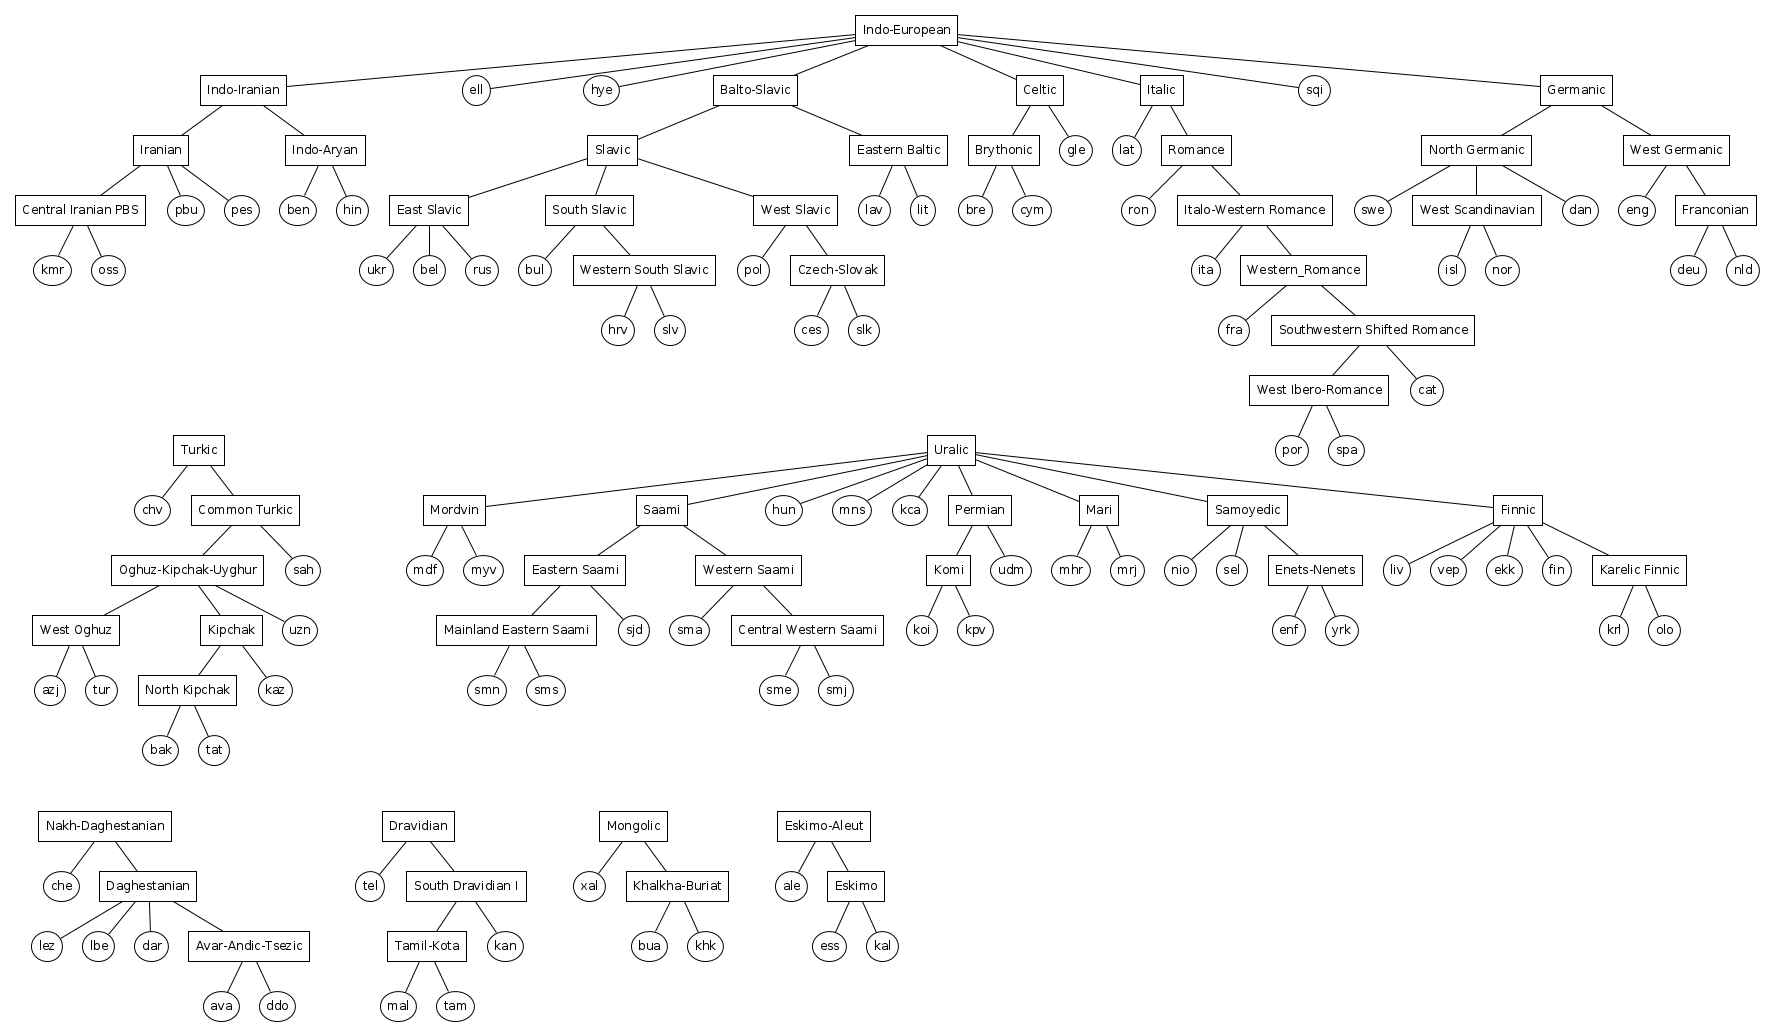
\includegraphics[width=\textwidth]{figures/glottolog-family-trees.png}
 \captionof{figure}{Reduced Glottolog family trees for NorthEuraLex 0.9}%
 \addtocounter{table}{-1} 
\end{center}

\newpage

\section{Summary of lexical flow gold standard}
This gold standard attempts to cover all contacts between languages in North\-Eu\-ra\-Lex 0.9, which implies that it also contains some contacts that were not discussed as part of any case study. For each attested language, the direct ancestor in the reduced Glottolog tree for all of NorthEuraLex is given. This first incoming arrow is not necessarily identical to the direct ancestor in the case studies, which are always based on a tree which is further reduced to only contain the languages spanned by the case study as leaves. All further arrows are due to contact, completely specifying all donor languages of lexical material in the respective language. Contacts between proto-languages are mentioned multiple times as influencing the descendants of the recipient language, with additional remarks specifying which ancestor of the current language was the recipient language.

\begin{center}
\footnotesize

\begin{longtable}{lll}
\hline\hline
\textbf{Language} & \textbf{Parent} & \textbf{Donor languages ($\simeq$ incoming arrows)}\\
\hline
\endfirsthead
\hline\hline
\textbf{Language} & \textbf{Parent} & \textbf{Donor languages ($\simeq$ incoming arrows)}\\
\hline
\endhead
\hline
\endfoot
\hline
\endlastfoot

\texttt{ben}: Bengali & Indo-Aryan & \\
\texttt{hin}: Hindi & Indo-Aryan & \texttt{pes}, \texttt{eng}\\
\texttt{pbu}: Pashto & Iranian & \texttt{pes}, \texttt{hin}, \texttt{arb}\\
\texttt{pes}: Persian & Iranian & \texttt{arb}\\
\texttt{kmr}: Northern Kurdish & Central Iranian PBS & \texttt{tur}, \texttt{arb}\\
\texttt{oss}: Ossetian & Central Iranian PBS & \texttt{ady}, \texttt{che}, Turkic, \texttt{oss}\\
\texttt{hye}: Armenian & Indo-European & \texttt{kat}, Iranian, \texttt{pes}\\
\texttt{ell}: Greek & Indo-European & \texttt{lat}, \texttt{tur}\\
\texttt{sqi}: Albanian & Indo-European & \texttt{ell}, \texttt{lat}, Slavic, \texttt{tur}\\
\texttt{lit}: Lithuanian & Eastern Baltic & \\
\texttt{lav}: Latvian & Eastern Baltic & \texttt{deu}, \texttt{rus}\\
\texttt{bul}: Bulgarian & South Slavic & \texttt{rus}, \texttt{tur}\\
\texttt{hrv}: Croatian & Western South Slavic & \\
\texttt{slv}: Slovene & Western South Slavic & \\
\texttt{slk}: Slovak & Czech-Slovak & \\
\texttt{ces}: Czech & Czech-Slovak & \\
\texttt{pol}: Polish & West Slavic & \texttt{lat}\\
\texttt{ukr}: Ukrainian & East Slavic & \texttt{pol}\\
\texttt{bel}: Belarusian & East Slavic & \texttt{pol}, \texttt{rus}\\
\texttt{rus}: Russian & East Slavic & \\
\texttt{isl}: Icelandic & West Scandinavian & \\
\texttt{nor}: Norwegian & West Scandinavian & \texttt{deu}, \texttt{dan}\\
\texttt{swe}: Swedish & North Germanic & \texttt{deu}\\
\texttt{dan}: Danish & North Germanic & \texttt{deu}\\
\texttt{deu}: German & Franconian & \texttt{lat} (via West Germanic)\\
\texttt{nld}: Dutch & Franconian & \texttt{lat} (via West Germanic), \texttt{fra}\\
\texttt{eng}: English & West Germanic & \texttt{lat} (via West Germanic),\\
 & & North Germanic, \texttt{fra}\\
\texttt{gle}: Irish & Celtic & \texttt{eng}\\
\texttt{cym}: Welsh & Brythonic & \texttt{lat}, \texttt{eng}\\
\texttt{bre}: Breton & Brythonic & \texttt{lat}, \texttt{fra}\\
\texttt{lat}: Latin & Italic & \\
\texttt{fra}: French & Western Romance & West Germanic, \texttt{ita}\\
\texttt{cat}: Catalan & SW Shifted Romance & \texttt{fra}, \texttt{spa}\\
\texttt{spa}: Spanish & West Ibero-Romance & \texttt{lat}, \texttt{arb}, \texttt{fra}\\
\texttt{por}: Portuguese & West Ibero-Romance & \texttt{lat}, \texttt{arb}\\
\texttt{ita}: Italian & Italo-Western Romance & \\
\texttt{ron}: Romanian & Romance & \texttt{sqi}, Slavic, \texttt{lat}, \texttt{hun}, \texttt{deu},\\
 & & \texttt{ell}, \texttt{tur}, \texttt{fra}\\
\hline
\texttt{fin}: Finnish & Finnic & E. Baltic (via Finnic), \texttt{swe}\\
\texttt{krl}: North Karelian & Karelic Finnic & E. Baltic (via Finnic), \texttt{rus}\\
\texttt{olo}: Olonets Karelian & Karelic Finnic & E. Baltic (via Finnic), \texttt{rus}\\
\texttt{vep}: Veps & Finnic & Eastern Baltic (via Finnic), \texttt{rus}\\
\texttt{ekk}: Estonian & Finnic & Eastern Baltic (via Finnic), \texttt{deu}, \texttt{rus}\\
\texttt{liv}: Livonian & Finnic & Eastern Baltic (via Finnic), \texttt{deu}, \texttt{lav}\\
\texttt{sma}: Southern Saami & Western Saami & Finnic and Germanic (via Saami),\\
& & N. Germanic (via W. Saami), \texttt{nor}\\
\texttt{smj}: Lule Saami & Central Western Saami & Finnic and Germanic (via Saami),\\
& & N. Germanic (via W. Saami), \texttt{swe}\\
\texttt{sme}: Northern Saami & Central Western Saami & Finnic and Germanic (via Saami),\\
& & N. Germanic (via W. Saami), \texttt{fin}\\
\texttt{smn}: Inari Saami & Mainland Eastern Saami & Finnic and Germanic (via Saami),\\ & & \texttt{fin}\\
\texttt{sms}: Skolt Saami & Mainland Eastern Saami & Finnic and Germanic (via Saami),\\
& & \texttt{krl}, \texttt{fin}, \texttt{rus}\\
\texttt{sjd}: Kildin Saami & Eastern Saami & Finnic and Germanic (via Saami),\\
& & \texttt{krl}, \texttt{rus}\\
\texttt{mrj}: Hill Mari & Mari &  \texttt{chv} (via Mari), \texttt{tat} (via Mari), \texttt{rus}\\
\texttt{mhr}: Meadow Mari & Mari & \texttt{chv} (via Mari), \texttt{tat} (via Mari)\\
\texttt{mdf}: Moksha & Mordvin & \\
\texttt{myv}: Erzya & Mordvin & \texttt{rus}\\
\texttt{udm}: Udmurt & Permian & \texttt{hun} (via Permian), \texttt{tat}, \texttt{bak}, \texttt{rus}\\
\texttt{koi}: Komi-Permyak & Komi & \texttt{rus}\\
\texttt{kpv}: Komi-Zyrian & Komi & \\
\texttt{hun}: Hungarian & Uralic & \texttt{kca}, Permian, Iranian, Turkic,\\
& & West Slavic, South Slavic, \texttt{deu}\\
\texttt{kca}: Northern Khanty & Uralic & \texttt{mns}, \texttt{hun}, \texttt{rus}\\
\texttt{mns}: Northern Mansi & Uralic & \texttt{kca}, \texttt{kpv}, \texttt{rus}\\
\texttt{yrk}: Tundra Nenets & Enets-Nenets & Turkic (via Samoyedic), \texttt{rus},\\
& & Tungusic (via Samoyedic), \texttt{kpv} \\
\texttt{enf}: Forest Enets & Enets-Nenets & Turkic (via Samoyedic), \texttt{rus},\\
& & Tungusic (via Samoyedic), \texttt{yrk} \\
\texttt{sel}: Northern Selkup & Samoyedic & Turkic (via Samoyedic), \texttt{rus},\\
& & Tungusic (via Samoyedic), \texttt{kca} \\
\texttt{nio}: Nganasan & Samoyedic & Turkic (via Samoyedic), \texttt{rus},\\
& & Tungusic (via Samoyedic) \\
\hline
\texttt{chv}: Chuvash & Turkic & \texttt{rus}\\
\texttt{tur}: Turkish & West Oghuz & \texttt{arb}, \texttt{pes}, \texttt{fra}, \texttt{ita}\\
\texttt{azj}: North Azerbaijani & West Oghuz & \texttt{arb}, \texttt{pes}\\
\texttt{uzn}: Northern Uzbek & Oghuz-Kipchak-Uyghur & \texttt{pes}\\
\texttt{kaz}: Kazakh & Kipchak & Mongolic, \texttt{rus}\\
\texttt{bak}: Bashkir & North Kipchak & \texttt{rus}\\
\texttt{tat}: Tatar & North Kipchak & \texttt{rus}\\
\texttt{sah}: Sakha & Common Turkic & \texttt{rus}, \texttt{bua}, \texttt{xal}\\
\hline
\texttt{khk}: Khalkha Mongolian & Khalkha-Buriat & Turkic, \texttt{rus}\\
\texttt{bua}: Buryat & Khalkha-Buriat & \texttt{rus}\\
\texttt{xal}: Kalmyk & Mongolic & Kipchak, \texttt{rus}\\
\hline
\texttt{evn}: Evenki & Tungusic & \texttt{bua}, \texttt{sah}, \texttt{rus}\\
\texttt{gld}: Nanai & Tungusic & \texttt{bua}, \texttt{rus}, \texttt{cmn}\\
\texttt{mnc}: Manchu & Tungusic & \texttt{khk}, \texttt{cmn}\\
\hline
\texttt{kor}: Korean & \textit{(none)} & Mongolic, Tungusic, \texttt{cmn}, \texttt{eng}\\
\hline
\texttt{jpn}: Japanese & \textit{(none)} & \texttt{cmn}, \texttt{eng}\\
\hline
\texttt{ain}: Hokkaido Ainu & \textit{(none)} & \texttt{niv}, \texttt{jpn}\\
\hline
\texttt{niv}: Nivkh & \textit{(none)} & \texttt{gld}, \texttt{rus}\\
\hline
\texttt{ykg}: Tundra Yukaghir & Yukaghir & Uralic (via Yukaghir), \texttt{evn} (via Yukaghir),\\ & & \texttt{sah} (via Yukaghir), \texttt{rus}\\
\texttt{yux}: Kolyma Yukaghir & Yukaghir & Uralic (via Yukaghir), \texttt{evn} (via Yukaghir),\\ & & \texttt{sah} (via Yukaghir), \texttt{rus}\\
\hline
\texttt{ckt}: Chukchi & Chukotko-Kamchatkan & Eskimo-Aleut (via CK)\\
\texttt{itl}: Itelmen & Chukotko-Kamchatkan & Eskimo-Aleut (via CK), \texttt{rus}\\
\hline
\texttt{ess}: Siberian Yupik & Eskimo & \texttt{rus}\\
\texttt{kal}: Kalaallisut & Eskimo & \texttt{dan}\\
\texttt{ale}: Aleut & Eskimo-Aleut & \texttt{rus}\\
\hline
\texttt{ket}: Ket & \textit{(none)} & \texttt{rus}\\
\hline
\texttt{kan}: Kannada & South Dravidian I & Indo-Aryan (via Dravidian), \texttt{eng}\\
\texttt{mal}: Malayalam & Tamil-Kota & Indo-Aryan (via Dravidian), \texttt{eng}\\
\texttt{tam}: Tamil & Tamil-Kota & Indo-Aryan (via Dravidian), \texttt{eng}\\
\texttt{tel}: Telugu & Dravidian & Indo-Aryan (via Dravidian), \texttt{eng}\\
\hline
\texttt{bsk}: Burushaski & \textit{(none)} & \texttt{hin}, Turkic\\
\hline
\texttt{kat}: Georgian & \textit{(none)} & \texttt{pes}, \texttt{azj}\\
\hline
\texttt{eus}: Basque & \textit{(none)} & \texttt{spa}\\
\hline
\texttt{abk}: Abkhaz & Abkhaz-Adyge & \texttt{kat}, \texttt{rus}\\
\texttt{ady}: Adyghe & Abkhaz-Adyge & \texttt{rus}, \texttt{azj}, Kipchak\\
\hline
\texttt{che}: Chechen & Nakh-Daghestanian & \texttt{oss}, \texttt{pes}, Kipchak, \texttt{rus}\\
\texttt{ava}: Avar & Avar-Andic-Tsezic & \texttt{kat}, \texttt{oss}, Kipchak, \texttt{arb}, \texttt{rus}\\
\texttt{ddo}: Tsez & Avar-Andic-Tsezic & \texttt{kat}, \texttt{azj}, \texttt{arb}, \texttt{rus}, \texttt{ava}\\
\texttt{lbe}: Lak & Daghestanian & \texttt{azj}, \texttt{arb}, \texttt{rus}, \texttt{ava}\\
\texttt{lez}: Lezgian & Daghestanian & \texttt{azj}, \texttt{arb}, \texttt{rus}\\
\texttt{dar}: Dargwa & Daghestanian & \texttt{azj}, Kipchak, \texttt{arb}, \texttt{rus}, \texttt{ava}\\
\hline
\texttt{arb}: Standard Arabic & Afro-Asiatic & \\
\texttt{heb}: Hebrew & Afro-Asiatic & Germanic, SW Shifted Romance\\
\hline
\texttt{cmn}: Mandarin Chinese & \textit{(none)} & \\
\end{longtable}
 \captionof{figure}{Gold standard for lexical flow, listing all incoming flows for each language}%
 \addtocounter{table}{-1}
\end{center}

\section{Concepts of NorthEuraLex 0.9}
The following table contains the full list of NorthEuraLex concepts in an order which is roughly grouped by semantic criteria, starting with body parts, then moving through landscape features towards plant and animal names, and so on. Internally, all concepts are identified by a German-language lemma with a rough part-of-speech annotation, which is given as the last column. Whenever concepts are referred to in the main text, they are instead referred to by the (sometimes annotated) English lemmas in the first column. The central column contains annotations which serve to disambiguate polysemous English glosses.

\begin{center}
\small
\begin{longtable}{lll}
\hline\hline
\textbf{Concept} & \textbf{Gloss and Explanation} & \textbf{Internal ID}\\
\hline
\endfirsthead
\hline\hline
\textbf{Concept} & \textbf{Gloss and Explanation} & \textbf{Internal ID}\\
\hline
\endhead
\hline
\endfoot
\hline
\endlastfoot

{\sc \lowercase{	EYE	}}	&	eye	\textit{\footnotesize [anatomy]}	&	Auge::N	\\
{\sc \lowercase{	EAR	}}	&	ear	\textit{\footnotesize [anatomy]}	&	Ohr::N	\\
{\sc \lowercase{	NOSE	}}	&	nose	\textit{\footnotesize [anatomy]}	&	Nase::N	\\
{\sc \lowercase{	MOUTH	}}	&	mouth	\textit{\footnotesize [anatomy]}	&	Mund::N	\\
{\sc \lowercase{	TOOTH	}}	&	tooth	\textit{\footnotesize (e.g. human incisor)}	&	Zahn::N	\\
{\sc \lowercase{	TONGUE	}}	&	tongue	\textit{\footnotesize [anatomy]}	&	Zunge::N	\\
{\sc \lowercase{	LIP	}}	&	lip	\textit{\footnotesize [anatomy]}	&	Lippe::N	\\
{\sc \lowercase{	CHEEK	}}	&	cheek	\textit{\footnotesize [anatomy]}	&	Wange::N	\\
{\sc \lowercase{	FACE	}}	&	face	\textit{\footnotesize (of a human)}	&	Gesicht::N	\\
{\sc \lowercase{	FOREHEAD	}}	&	forehead	\textit{\footnotesize (of a human)}	&	Stirn::N	\\
{\sc \lowercase{	HAIR	}}	&	hair	\textit{\footnotesize (of human head)}	&	Haar::N	\\
{\sc \lowercase{	MOUSTACHE	}}	&	moustache	\textit{\footnotesize (of a man)}	&	Schnurrbart::N	\\
{\sc \lowercase{	BEARD	}}	&	beard	\textit{\footnotesize (generic)}	&	Bart::N	\\
{\sc \lowercase{	CHIN	}}	&	chin	\textit{\footnotesize [anatomy]}	&	Kinn::N	\\
{\sc \lowercase{	JAW	}}	&	jaw	\textit{\footnotesize [anatomy]}	&	Kiefer[Anatomie]::N	\\
{\sc \lowercase{	THROAT	}}	&	throat	\textit{\footnotesize (from inside)}	&	Kehle::N	\\
{\sc \lowercase{	NECK	}}	&	neck	\textit{\footnotesize (from outside)}	&	Hals::N	\\
{\sc \lowercase{	NAPE \footnotesize (OF NECK)	}}	&	nape	\textit{\footnotesize (back side of neck)}	&	Genick::N	\\
{\sc \lowercase{	HEAD	}}	&	head	\textit{\footnotesize (e.g. of a human)}	&	Kopf::N	\\
{\sc \lowercase{	BACK	}}	&	back	\textit{\footnotesize (of a human)}	&	Rücken::N	\\
{\sc \lowercase{	BELLY	}}	&	belly	\textit{\footnotesize (of a human)}	&	Bauch::N	\\
{\sc \lowercase{	NAVEL	}}	&	navel	\textit{\footnotesize [anatomy]}	&	Nabel::N	\\
{\sc \lowercase{	BREAST	}}	&	bosom	\textit{\footnotesize (female breast)}	&	Busen::N	\\
{\sc \lowercase{	CHEST	}}	&	breast	\textit{\footnotesize (e.g. of a man)}	&	Brust::N	\\
{\sc \lowercase{	SHOULDER	}}	&	shoulder	\textit{\footnotesize [anatomy]}	&	Schulter::N	\\
{\sc \lowercase{	ARM	}}	&	arm	\textit{\footnotesize (of a human)}	&	Arm::N	\\
{\sc \lowercase{	ELBOW	}}	&	elbow	\textit{\footnotesize (of a human)}	&	Ellenbogen::N	\\
{\sc \lowercase{	HAND	}}	&	hand	\textit{\footnotesize (of a human)}	&	Hand::N	\\
{\sc \lowercase{	PALM OF HAND	}}	&	palm	\textit{\footnotesize [anatomy]}	&	Handfläche::N	\\
{\sc \lowercase{	FINGER	}}	&	finger	\textit{\footnotesize (of a human)}	&	Finger::N	\\
{\sc \lowercase{	FINGERNAIL	}}	&	fingernail	\textit{\footnotesize [anatomy]}	&	Fingernagel::N	\\
{\sc \lowercase{	\footnotesize FINGERNAIL OR TOENAIL	}}	&	nail	\textit{\footnotesize [anatomy]}	&	Nagel[Anatomie]::N	\\
{\sc \lowercase{	TOE	}}	&	toe	\textit{\footnotesize (of a human)}	&	Zeh::N	\\
{\sc \lowercase{	FOOT	}}	&	foot	\textit{\footnotesize (of a human)}	&	Fuß::N	\\
{\sc \lowercase{	HEEL	}}	&	heel	\textit{\footnotesize [anatomy]}	&	Ferse::N	\\
{\sc \lowercase{	KNEE	}}	&	knee	\textit{\footnotesize [anatomy]}	&	Knie::N	\\
{\sc \lowercase{	THIGH	}}	&	thigh	\textit{\footnotesize [anatomy]}	&	Oberschenkel::N	\\
{\sc \lowercase{	LEG	}}	&	leg	\textit{\footnotesize (of a human)}	&	Bein::N	\\
{\sc \lowercase{	BODY	}}	&	body	\textit{\footnotesize (of a living organism)}	&	Körper::N	\\
{\sc \lowercase{	SKIN	}}	&	skin	\textit{\footnotesize (of a human)}	&	Haut::N	\\
{\sc \lowercase{	BLOOD	}}	&	blood	\textit{\footnotesize (fluid)}	&	Blut::N	\\
{\sc \lowercase{	VEIN	}}	&	vein	\textit{\footnotesize [anatomy]}	&	Ader::N	\\
{\sc \lowercase{	TENDON	}}	&	sinew	\textit{\footnotesize [anatomy]}	&	Sehne::N	\\
{\sc \lowercase{	BONE	}}	&	bone	\textit{\footnotesize [anatomy]}	&	Knochen::N	\\
{\sc \lowercase{	BRAIN	}}	&	brain	\textit{\footnotesize [anatomy]}	&	Gehirn::N	\\
{\sc \lowercase{	HEART	}}	&	heart	\textit{\footnotesize [anatomy]}	&	Herz::N	\\
{\sc \lowercase{	STOMACH	}}	&	stomach	\textit{\footnotesize [anatomy]}	&	Magen::N	\\
{\sc \lowercase{	LIVER	}}	&	liver	\textit{\footnotesize [anatomy]}	&	Leber::N	\\
{\sc \lowercase{	BREATH	}}	&	breath	\textit{\footnotesize (breathing)}	&	Atem::N	\\
{\sc \lowercase{	HUNGER	}}	&	hunger	\textit{\footnotesize (condition)}	&	Hunger::N	\\
{\sc \lowercase{	TEAR \footnotesize (OF EYE)	}}	&	tear	\textit{\footnotesize (drop of fluid)}	&	Träne::N	\\
{\sc \lowercase{	TASTE	}}	&	flavour	\textit{\footnotesize (of something)}	&	Geschmack::N	\\
{\sc \lowercase{	FLAVOR	}}	&	odour	\textit{\footnotesize (of something)}	&	Geruch::N	\\
{\sc \lowercase{	SLEEP \footnotesize (STATE)	}}	&	sleep	\textit{\footnotesize (condition)}	&	Schlaf::N	\\
{\sc \lowercase{	DREAM	}}	&	dream	\textit{\footnotesize (while sleeping)}	&	Traum::N	\\
{\sc \lowercase{	SKY	}}	&	sky	\textit{\footnotesize (visible)}	&	Himmel::N	\\
{\sc \lowercase{	SUN	}}	&	sun	\textit{\footnotesize (celestial body)}	&	Sonne::N	\\
{\sc \lowercase{	MOON	}}	&	moon	\textit{\footnotesize (celestial body)}	&	Mond::N	\\
{\sc \lowercase{	STAR	}}	&	star	\textit{\footnotesize (in the night sky)}	&	Stern::N	\\
{\sc \lowercase{	AIR	}}	&	air	\textit{\footnotesize (where birds fly)}	&	Luft::N	\\
{\sc \lowercase{	WIND	}}	&	wind	\textit{\footnotesize (outside)}	&	Wind::N	\\
{\sc \lowercase{	WAVE	}}	&	wave	\textit{\footnotesize (on water)}	&	Welle::N	\\
{\sc \lowercase{	WATER	}}	&	water	\textit{\footnotesize (cold water)}	&	Wasser::N	\\
{\sc \lowercase{	ROCK	}}	&	stone	\textit{\footnotesize (substance)}	&	Stein::N	\\
{\sc \lowercase{	GROUND	}}	&	ground	\textit{\footnotesize (soil, earth)}	&	Boden::N	\\
{\sc \lowercase{	EARTH \footnotesize (SOIL)	}}	&	earth	\textit{\footnotesize (substance)}	&	Erde::N	\\
{\sc \lowercase{	DUST	}}	&	dust	\textit{\footnotesize (settled)}	&	Staub::N	\\
{\sc \lowercase{	SMOKE \footnotesize (EXHAUST)	}}	&	smoke	\textit{\footnotesize (from a fire)}	&	Rauch::N	\\
{\sc \lowercase{	SPARK	}}	&	spark	\textit{\footnotesize (from a fire)}	&	Funke::N	\\
{\sc \lowercase{	FIRE	}}	&	fire	\textit{\footnotesize (flames)}	&	Feuer::N	\\
{\sc \lowercase{	LIGHT \footnotesize (RADIATION)	}}	&	light	\textit{\footnotesize (from a natural source)}	&	Licht::N	\\
{\sc \lowercase{	SHADE	}}	&	shadow	\textit{\footnotesize (shady place)}	&	Schatten::N	\\
{\sc \lowercase{	WEATHER	}}	&	weather		&	Wetter::N	\\
{\sc \lowercase{	FOG	}}	&	fog		&	Nebel::N	\\
{\sc \lowercase{	CLOUD	}}	&	cloud	\textit{\footnotesize (bright)}	&	Wolke::N	\\
{\sc \lowercase{	RAIN \footnotesize (PRECIPITATION)	}}	&	rain	\textit{\footnotesize (falling)}	&	Regen::N	\\
{\sc \lowercase{	SNOW	}}	&	snow	\textit{\footnotesize (on the ground)}	&	Schnee::N	\\
{\sc \lowercase{	ICE	}}	&	ice	\textit{\footnotesize (natural substance)}	&	Eis::N	\\
{\sc \lowercase{	FROST	}}	&	frost	\textit{\footnotesize (freezing temperature)}	&	Frost::N	\\
{\sc \lowercase{	CHILL	}}	&	chill	\textit{\footnotesize (low temperature)}	&	Kälte::N	\\
{\sc \lowercase{	HEAT	}}	&	heat	\textit{\footnotesize (high temperature)}	&	Hitze::N	\\
{\sc \lowercase{	HOARFROST	}}	&	hoarfrost		&	Raureif::N	\\
{\sc \lowercase{	RAINBOW	}}	&	rainbow		&	Regenbogen::N	\\
{\sc \lowercase{	THUNDER	}}	&	thunder	\textit{\footnotesize (during thunderstorm)}	&	Donner::N	\\
{\sc \lowercase{	CURRENT	}}	&	current	\textit{\footnotesize (of a river)}	&	Strömung::N	\\
{\sc \lowercase{	DROP \footnotesize (OF LIQUID)	}}	&	drop	\textit{\footnotesize (e.g. water)}	&	Tropfen::N	\\
{\sc \lowercase{	FOAM	}}	&	foam	\textit{\footnotesize (on liquid)}	&	Schaum::N	\\
{\sc \lowercase{	DIRT	}}	&	dirt	\textit{\footnotesize (on objects)}	&	Schmutz::N	\\
{\sc \lowercase{	LAKE	}}	&	lake		&	See::N	\\
{\sc \lowercase{	SWAMP	}}	&	swamp	\textit{\footnotesize (impassable wet land)}	&	Sumpf::N	\\
{\sc \lowercase{	MOOR	}}	&	moor	\textit{\footnotesize (wasteland covered by heath)}	&	Moor::N	\\
{\sc \lowercase{	MEADOW	}}	&	meadow	\textit{\footnotesize (land covered with grass)}	&	Wiese::N	\\
{\sc \lowercase{	FOREST	}}	&	forest		&	Wald::N	\\
{\sc \lowercase{	HILL	}}	&	hill	\textit{\footnotesize (possibly wooded)}	&	Hügel::N	\\
{\sc \lowercase{	ELEVATION	}}	&	elevation	\textit{\footnotesize (of the ground)}	&	Anhöhe::N	\\
{\sc \lowercase{	MOUNTAIN	}}	&	mountain	\textit{\footnotesize (woodless)}	&	Berg::N	\\
{\sc \lowercase{	SUMMIT	}}	&	summit	\textit{\footnotesize (of a mountain)}	&	Gipfel::N	\\
{\sc \lowercase{	CAVE	}}	&	cave	\textit{\footnotesize (in a mountain)}	&	Höhle::N	\\
{\sc \lowercase{	PRECIPICE	}}	&	slope	\textit{\footnotesize (of a mountain)}	&	Abhang::N	\\
{\sc \lowercase{	SPRING \footnotesize (OF WATER)	}}	&	source	\textit{\footnotesize (of a river)}	&	Quelle::N	\\
{\sc \lowercase{	BROOK	}}	&	brook	\textit{\footnotesize (small river)}	&	Bach::N	\\
{\sc \lowercase{	RIVER	}}	&	river	\textit{\footnotesize (larger river)}	&	Fluss::N	\\
{\sc \lowercase{	SHORE	}}	&	shore	\textit{\footnotesize (of a lake)}	&	Ufer::N	\\
{\sc \lowercase{	COAST	}}	&	coast	\textit{\footnotesize (seashore)}	&	Küste::N	\\
{\sc \lowercase{	MAINLAND	}}	&	land	\textit{\footnotesize (as opposed to sea)}	&	Festland::N	\\
{\sc \lowercase{	SEA	}}	&	sea		&	Meer::N	\\
{\sc \lowercase{	BAY	}}	&	cove, bay	\textit{\footnotesize (small coastal inlet)}	&	Bucht::N	\\
{\sc \lowercase{	ISLAND	}}	&	island		&	Insel::N	\\
{\sc \lowercase{	FLOWER	}}	&	flower		&	Blume::N	\\
{\sc \lowercase{	GRASS	}}	&	grass	\textit{\footnotesize (ground cover)}	&	Gras::N	\\
{\sc \lowercase{	ROOT	}}	&	root	\textit{\footnotesize (of a plant)}	&	Wurzel::N	\\
{\sc \lowercase{	TREE	}}	&	tree	\textit{\footnotesize (plant)}	&	Baum::N	\\
{\sc \lowercase{	TREE TRUNK	}}	&	trunk	\textit{\footnotesize (of a tree)}	&	Stamm::N	\\
{\sc \lowercase{	BARK	}}	&	bark	\textit{\footnotesize (of a tree)}	&	Rinde::N	\\
{\sc \lowercase{	BRANCH	}}	&	limb	\textit{\footnotesize (of a tree)}	&	Ast::N	\\
{\sc \lowercase{	TWIG	}}	&	twig	\textit{\footnotesize (of a tree)}	&	Zweig::N	\\
{\sc \lowercase{	LEAF	}}	&	leaf	\textit{\footnotesize (of a plant)}	&	Blatt::N	\\
{\sc \lowercase{	BIRCH	}}	&	birch		&	Birke::N	\\
{\sc \lowercase{	PINE	}}	&	pine	\textit{\footnotesize (pine tree)}	&	Kiefer[Baum]::N	\\
{\sc \lowercase{	WILLOW	}}	&	willow		&	Weide[Baum]::N	\\
{\sc \lowercase{	FIR	}}	&	fir		&	Tanne::N	\\
{\sc \lowercase{	HORN \footnotesize (ANATOMY)	}}	&	horn	\textit{\footnotesize (of an animal)}	&	Horn::N	\\
{\sc \lowercase{	FEATHER	}}	&	feather	\textit{\footnotesize (of a bird)}	&	Feder::N	\\
{\sc \lowercase{	FUR	}}	&	fur	\textit{\footnotesize (of an animal)}	&	Fell::N	\\
{\sc \lowercase{	WING	}}	&	wing	\textit{\footnotesize (of a bird)}	&	Flügel::N	\\
{\sc \lowercase{	CLAW	}}	&	claw	\textit{\footnotesize (e.g. of a bird)}	&	Klaue::N	\\
{\sc \lowercase{	PAW	}}	&	paw	\textit{\footnotesize (e.g. of a cat)}	&	Kralle::N	\\
{\sc \lowercase{	TAIL	}}	&	tail	\textit{\footnotesize (e.g. of a dog)}	&	Schwanz::N	\\
{\sc \lowercase{	EGG	}}	&	egg	\textit{\footnotesize (e.g. of a bird)}	&	Ei::N	\\
{\sc \lowercase{	NEST	}}	&	nest	\textit{\footnotesize (e.g. of a bird)}	&	Nest::N	\\
{\sc \lowercase{	LAIR	}}	&	lair	\textit{\footnotesize (e.g. of a fox)}	&	Bau::N	\\
{\sc \lowercase{	ANIMAL	}}	&	animal		&	Tier::N	\\
{\sc \lowercase{	FLOCK \footnotesize (OF SHEEP)	}}	&	flock	\textit{\footnotesize (e.g. of sheep)}	&	Herde::N	\\
{\sc \lowercase{	COW	}}	&	cow		&	Kuh::N	\\
{\sc \lowercase{	BULL	}}	&	bull	\textit{\footnotesize (male bovine)}	&	Bulle::N	\\
{\sc \lowercase{	HORSE	}}	&	horse		&	Pferd::N	\\
{\sc \lowercase{	SHEEP	}}	&	sheep		&	Schaf::N	\\
{\sc \lowercase{	PIG	}}	&	pig		&	Schwein::N	\\
{\sc \lowercase{	DOG	}}	&	dog		&	Hund::N	\\
{\sc \lowercase{	CAT	}}	&	cat		&	Katze::N	\\
{\sc \lowercase{	BEAR	}}	&	bear		&	Bär::N	\\
{\sc \lowercase{	SQUIRREL	}}	&	squirrel		&	Eichhörnchen::N	\\
{\sc \lowercase{	ELK	}}	&	elk		&	Elch::N	\\
{\sc \lowercase{	FOX	}}	&	fox		&	Fuchs::N	\\
{\sc \lowercase{	HARE	}}	&	hare		&	Hase::N	\\
{\sc \lowercase{	MOUSE	}}	&	mouse		&	Maus::N	\\
{\sc \lowercase{	WOLF	}}	&	wolf		&	Wolf::N	\\
{\sc \lowercase{	BIRD	}}	&	bird		&	Vogel::N	\\
{\sc \lowercase{	SWARM	}}	&	swarm	\textit{\footnotesize (e.g. of birds)}	&	Schwarm::N	\\
{\sc \lowercase{	CHICKEN	}}	&	chicken		&	Huhn::N	\\
{\sc \lowercase{	ROOSTER	}}	&	cock	\textit{\footnotesize (male chicken)}	&	Hahn::N	\\
{\sc \lowercase{	GOOSE	}}	&	goose		&	Gans::N	\\
{\sc \lowercase{	EAGLE	}}	&	eagle		&	Adler::N	\\
{\sc \lowercase{	DUCK	}}	&	duck		&	Ente::N	\\
{\sc \lowercase{	OWL	}}	&	owl		&	Eule::N	\\
{\sc \lowercase{	CRANE	}}	&	crane		&	Kranich::N	\\
{\sc \lowercase{	CROW	}}	&	crow		&	Krähe::N	\\
{\sc \lowercase{	CUCKOO	}}	&	cuckoo		&	Kuckuck::N	\\
{\sc \lowercase{	SWAN	}}	&	swan		&	Schwan::N	\\
{\sc \lowercase{	FISH	}}	&	fish		&	Fisch::N	\\
{\sc \lowercase{	PERCH \footnotesize (FISH)	}}	&	perch		&	Barsch::N	\\
{\sc \lowercase{	PIKE \footnotesize (FISH)	}}	&	pike		&	Hecht::N	\\
{\sc \lowercase{	SNAKE	}}	&	snake		&	Schlange[Tier]::N	\\
{\sc \lowercase{	WORM	}}	&	worm		&	Wurm::N	\\
{\sc \lowercase{	SPIDER	}}	&	spider		&	Spinne::N	\\
{\sc \lowercase{	ANT	}}	&	ant		&	Ameise::N	\\
{\sc \lowercase{	LOUSE	}}	&	louse		&	Laus::N	\\
{\sc \lowercase{	MOSQUITO	}}	&	gnat		&	Mücke::N	\\
{\sc \lowercase{	FLY \footnotesize (INSECT)	}}	&	fly	\textit{\footnotesize (insect)}	&	Fliege::N	\\
{\sc \lowercase{	BUTTERFLY	}}	&	butterfly		&	Schmetterling::N	\\
{\sc \lowercase{	BERRY	}}	&	berry	\textit{\footnotesize (generic term)}	&	Beere::N	\\
{\sc \lowercase{	APPLE	}}	&	apple		&	Apfel::N	\\
{\sc \lowercase{	MUSHROOM	}}	&	mushroom	\textit{\footnotesize (generic term)}	&	Pilz::N	\\
{\sc \lowercase{	ONION	}}	&	onion	\textit{\footnotesize (edible)}	&	Zwiebel::N	\\
{\sc \lowercase{	SEED	}}	&	seed	\textit{\footnotesize (fertilized grain)}	&	Saat::N	\\
{\sc \lowercase{	GRAIN \footnotesize (SINGLE)	}}	&	grain	\textit{\footnotesize (single grain)}	&	Korn::N	\\
{\sc \lowercase{	HAY	}}	&	hay		&	Heu::N	\\
{\sc \lowercase{	SKIN \footnotesize (OF FRUIT)	}}	&	peel, husk	\textit{\footnotesize (e.g. of an apple)}	&	Schale::N	\\
{\sc \lowercase{	PIT \footnotesize (POTHOLE)	}}	&	pit	\textit{\footnotesize (hole in the ground)}	&	Grube::N	\\
{\sc \lowercase{	TRAP \footnotesize (PITFALL)	}}	&	trap	\textit{\footnotesize (e.g. mouse trap)}	&	Falle::N	\\
{\sc \lowercase{	NOOSE	}}	&	noose	\textit{\footnotesize (e.g. on a rope)}	&	Schlinge::N	\\
{\sc \lowercase{	TRACK \footnotesize (OF ANIMAL)	}}	&	track	\textit{\footnotesize (e.g. of an animal)}	&	Spur::N	\\
{\sc \lowercase{	ASH	}}	&	ash	\textit{\footnotesize (solid remains of a fire)}	&	Asche::N	\\
{\sc \lowercase{	FILTH	}}	&	filth	\textit{\footnotesize (that which soils or defiles)}	&	Dreck::N	\\
{\sc \lowercase{	IRON	}}	&	iron	\textit{\footnotesize (metal)}	&	Eisen::N	\\
{\sc \lowercase{	GOLD	}}	&	gold	\textit{\footnotesize (metal)}	&	Gold::N	\\
{\sc \lowercase{	SILVER	}}	&	silver	\textit{\footnotesize (metal)}	&	Silber::N	\\
{\sc \lowercase{	CHARCOAL	}}	&	coal	\textit{\footnotesize (combustible substance)}	&	Kohle::N	\\
{\sc \lowercase{	GLASS	}}	&	glass	\textit{\footnotesize (transparent substance)}	&	Glas::N	\\
{\sc \lowercase{	CLAY	}}	&	clay	\textit{\footnotesize (ductile material)}	&	Lehm::N	\\
{\sc \lowercase{	SAND	}}	&	sand	\textit{\footnotesize (material)}	&	Sand::N	\\
{\sc \lowercase{	PERSON	}}	&	human	\textit{\footnotesize (human being)}	&	Mensch::N	\\
{\sc \lowercase{	MAN	}}	&	man	\textit{\footnotesize (adult male human)}	&	Mann::N	\\
{\sc \lowercase{	WOMAN	}}	&	woman		&	Frau::N	\\
{\sc \lowercase{	CHILD \footnotesize (YOUNG HUMAN)	}}	&	child	\textit{\footnotesize (e.g. 10 years old)}	&	Kind::N	\\
{\sc \lowercase{	BOY	}}	&	boy	\textit{\footnotesize (male child)}	&	Junge::N	\\
{\sc \lowercase{	GIRL	}}	&	girl	\textit{\footnotesize (female child)}	&	Mädchen::N	\\
{\sc \lowercase{	FAMILY	}}	&	family	\textit{\footnotesize (relatives living together)}	&	Familie::N	\\
{\sc \lowercase{	GRANDFATHER	}}	&	grandfather	\textit{\footnotesize (e.g. father's father)}	&	Großvater::N	\\
{\sc \lowercase{	GRANDMOTHER	}}	&	grandmother	\textit{\footnotesize (e.g. father's mother)}	&	Großmutter::N	\\
{\sc \lowercase{	PARENTS	}}	&	parents		&	Eltern::N	\\
{\sc \lowercase{	FATHER	}}	&	father		&	Vater::N	\\
{\sc \lowercase{	MOTHER	}}	&	mother		&	Mutter::N	\\
{\sc \lowercase{	SON	}}	&	son		&	Sohn::N	\\
{\sc \lowercase{	DAUGHTER	}}	&	daughter		&	Tochter::N	\\
{\sc \lowercase{	BROTHER	}}	&	brother	\textit{\footnotesize (e.g. elder brother)}	&	Bruder::N	\\
{\sc \lowercase{	SISTER	}}	&	sister	\textit{\footnotesize (e.g. elder sister)}	&	Schwester::N	\\
{\sc \lowercase{	UNCLE	}}	&	uncle	\textit{\footnotesize (e.g. father's brother)}	&	Onkel::N	\\
{\sc \lowercase{	AUNT	}}	&	aunt	\textit{\footnotesize (e.g. father's sister)}	&	Tante::N	\\
{\sc \lowercase{	HUSBAND	}}	&	husband	\textit{\footnotesize (male spouse)}	&	Ehemann::N	\\
{\sc \lowercase{	WIFE	}}	&	wife	\textit{\footnotesize (female spouse)}	&	Ehefrau::N	\\
{\sc \lowercase{	JOY	}}	&	joy	\textit{\footnotesize (emotion)}	&	Freude::N	\\
{\sc \lowercase{	LAUGHTER	}}	&	laughter		&	Gelächter::N	\\
{\sc \lowercase{	HAPPINESS	}}	&	happiness		&	Glück::N	\\
{\sc \lowercase{	GRIEF	}}	&	grief	\textit{\footnotesize (sorrow, sadness)}	&	Kummer::N	\\
{\sc \lowercase{	LONGING	}}	&	wish	\textit{\footnotesize (longing)}	&	Wunsch::N	\\
{\sc \lowercase{	DESIRE	}}	&	desire	\textit{\footnotesize (to have something)}	&	Lust::N	\\
{\sc \lowercase{	SPIRIT	}}	&	spirit	\textit{\footnotesize (inner energy of a being)}	&	Geist::N	\\
{\sc \lowercase{	THOUGHT	}}	&	thought		&	Gedanke::N	\\
{\sc \lowercase{	MEMORY	}}	&	memory	\textit{\footnotesize (human ability)}	&	Gedächtnis::N	\\
{\sc \lowercase{	MIND	}}	&	mind	\textit{\footnotesize (ability for rational thought)}	&	Verstand::N	\\
{\sc \lowercase{	MEANING	}}	&	meaning	\textit{\footnotesize (denotation)}	&	Sinn::N	\\
{\sc \lowercase{	REASON	}}	&	reason	\textit{\footnotesize (motive, rationale)}	&	Grund::N	\\
{\sc \lowercase{	TRUTH	}}	&	truth		&	Wahrheit::N	\\
{\sc \lowercase{	CONVERSATION	}}	&	talk	\textit{\footnotesize (conversation)}	&	Gespräch::N	\\
{\sc \lowercase{	FAIRY TALE	}}	&	fairy tale		&	Märchen::N	\\
{\sc \lowercase{	STORY	}}	&	story	\textit{\footnotesize (oral narration)}	&	Erzählung::N	\\
{\sc \lowercase{	MESSAGE	}}	&	message		&	Nachricht::N	\\
{\sc \lowercase{	NEWS	}}	&	news		&	Neuigkeit::N	\\
{\sc \lowercase{	NAME	}}	&	name	\textit{\footnotesize (of a person)}	&	Name::N	\\
{\sc \lowercase{	RIDDLE	}}	&	puzzle	\textit{\footnotesize (riddle)}	&	Rätsel::N	\\
{\sc \lowercase{	SPEECH	}}	&	speech	\textit{\footnotesize (long oral message)}	&	Rede::N	\\
{\sc \lowercase{	LANGUAGE	}}	&	language		&	Sprache::N	\\
{\sc \lowercase{	VOICE	}}	&	voice	\textit{\footnotesize (sounds uttered by vocal cords)}	&	Stimme::N	\\
{\sc \lowercase{	WORD	}}	&	word	\textit{\footnotesize (unit of language)}	&	Wort::N	\\
{\sc \lowercase{	SIGN	}}	&	sign	\textit{\footnotesize (object bearing a message)}	&	Zeichen::N	\\
{\sc \lowercase{	CALL \footnotesize (APPEAL)	}}	&	call	\textit{\footnotesize (appeal)}	&	Ruf::N	\\
{\sc \lowercase{	NOISE	}}	&	noise	\textit{\footnotesize (unwanted loud sounds)}	&	Lärm::N	\\
{\sc \lowercase{	SOUND OR NOISE	}}	&	sound	\textit{\footnotesize (sensation perceived by ear)}	&	Laut::N	\\
{\sc \lowercase{	TONE \footnotesize (MUSIC)	}}	&	tone	\textit{\footnotesize (sound of a specific pitch)}	&	Ton::N	\\
{\sc \lowercase{	SONG	}}	&	song		&	Lied::N	\\
{\sc \lowercase{	QUIET	}}	&	calm	\textit{\footnotesize (absence of disturbances)}	&	Ruhe::N	\\
{\sc \lowercase{	PEOPLE \footnotesize (SEVERAL)	}}	&	people	\textit{\footnotesize (many persons)}	&	Leute::N	\\
{\sc \lowercase{	PEOPLE	}}	&	nation	\textit{\footnotesize (defined by common culture)}	&	Volk::N	\\
{\sc \lowercase{	WORK \footnotesize (LABOUR)	}}	&	work	\textit{\footnotesize (employment)}	&	Arbeit::N	\\
{\sc \lowercase{	GUEST	}}	&	guest		&	Gast::N	\\
{\sc \lowercase{	GIFT	}}	&	gift		&	Geschenk::N	\\
{\sc \lowercase{	GAME	}}	&	game	\textit{\footnotesize (playful activity)}	&	Spiel::N	\\
{\sc \lowercase{	COMPANIONSHIP	}}	&	company	\textit{\footnotesize (companionship)}	&	Gesellschaft::N	\\
{\sc \lowercase{	HELP	}}	&	help		&	Hilfe::N	\\
{\sc \lowercase{	FRIEND	}}	&	friend	\textit{\footnotesize (enjoyable company)}	&	Freund::N	\\
{\sc \lowercase{	COMPANION	}}	&	companion	\textit{\footnotesize (one spends time with)}	&	Kamerad::N	\\
{\sc \lowercase{	MATTER \footnotesize (AFFAIR)	}}	&	matter	\textit{\footnotesize (affair)}	&	Angelegenheit::N	\\
{\sc \lowercase{	COUNT \footnotesize (NUMBER)	}}	&	count	\textit{\footnotesize (quantity counted)}	&	Anzahl::N	\\
{\sc \lowercase{	KIND \footnotesize (THING)	}}	&	sort	\textit{\footnotesize (type)}	&	Art::N	\\
{\sc \lowercase{	PIECE	}}	&	piece	\textit{\footnotesize (separable part)}	&	Stück::N	\\
{\sc \lowercase{	PART	}}	&	part	\textit{\footnotesize (fraction of a whole)}	&	Teil::N	\\
{\sc \lowercase{	HALF	}}	&	half	\textit{\footnotesize (of a quantity)}	&	Hälfte::N	\\
{\sc \lowercase{	CIRCLE	}}	&	circle	\textit{\footnotesize (geometric figure)}	&	Kreis::N	\\
{\sc \lowercase{	CROSS	}}	&	cross	\textit{\footnotesize (geometric figure)}	&	Kreuz::N	\\
{\sc \lowercase{	LINE	}}	&	line	\textit{\footnotesize (geometric figure)}	&	Linie::N	\\
{\sc \lowercase{	STROKE \footnotesize (OF PEN)	}}	&	stroke	\textit{\footnotesize (with writing implement)}	&	Strich::N	\\
{\sc \lowercase{	GAP	}}	&	gap	\textit{\footnotesize (between objects)}	&	Abstand::N	\\
{\sc \lowercase{	DISTANCE	}}	&	distance	\textit{\footnotesize (between two points)}	&	Entfernung::N	\\
{\sc \lowercase{	AREA	}}	&	area	\textit{\footnotesize (extent of surface, region)}	&	Gegend::N	\\
{\sc \lowercase{	SPACE \footnotesize (FREE)	}}	&	space	\textit{\footnotesize (available space, e.g. in closet)}	&	Platz::N	\\
{\sc \lowercase{	PLACE \footnotesize (POSITION)	}}	&	place	\textit{\footnotesize (location, position)}	&	Ort::N	\\
{\sc \lowercase{	SIDE \footnotesize (OF OBJECT)	}}	&	side	\textit{\footnotesize (of an object)}	&	Seite::N	\\
{\sc \lowercase{	MIDDLE	}}	&	middle	\textit{\footnotesize (central part of something)}	&	Mitte::N	\\
{\sc \lowercase{	ITEM \footnotesize (TOUCHABLE)	}}	&	item	\textit{\footnotesize (physical object)}	&	Gegenstand::N	\\
{\sc \lowercase{	THING	}}	&	thing	\textit{\footnotesize (distinct entity)}	&	Sache::N	\\
{\sc \lowercase{	FRINGE	}}	&	fringe	\textit{\footnotesize (peripheral part)}	&	Rand::N	\\
{\sc \lowercase{	EDGE	}}	&	edge	\textit{\footnotesize (sharp terminating border)}	&	Kante::N	\\
{\sc \lowercase{	CORNER \footnotesize (OUTSIDE)	}}	&	corner	\textit{\footnotesize (external angle)}	&	Ecke::N	\\
{\sc \lowercase{	TIP \footnotesize (OF OBJECT)	}}	&	tip	\textit{\footnotesize (of a pointy object)}	&	Spitze::N	\\
{\sc \lowercase{	END \footnotesize (OF SPACE)	}}	&	end	\textit{\footnotesize (of a long object)}	&	Ende::N	\\
{\sc \lowercase{	HOLE	}}	&	hole	\textit{\footnotesize (in an object)}	&	Loch::N	\\
{\sc \lowercase{	CORNER	}}	&	angle	\textit{\footnotesize (internal, e.g. of a room)}	&	Winkel::N	\\
{\sc \lowercase{	PATTERN	}}	&	pattern	\textit{\footnotesize (regular repeated elements)}	&	Muster::N	\\
{\sc \lowercase{	SIZE \footnotesize (OF OBJECT)	}}	&	size	\textit{\footnotesize (dimensions of an object)}	&	Größe::N	\\
{\sc \lowercase{	LENGTH	}}	&	length		&	Länge::N	\\
{\sc \lowercase{	HEIGHT	}}	&	height		&	Höhe::N	\\
{\sc \lowercase{	WEIGHT	}}	&	weight	\textit{\footnotesize (mass as measured)}	&	Gewicht::N	\\
{\sc \lowercase{	AMOUNT	}}	&	amount	\textit{\footnotesize (quantity of a material)}	&	Menge::N	\\
{\sc \lowercase{	HEAP	}}	&	heap		&	Haufen::N	\\
{\sc \lowercase{	ROW \footnotesize (OF OBJECTS)	}}	&	row	\textit{\footnotesize (line of objects)}	&	Reihe::N	\\
{\sc \lowercase{	BOAT	}}	&	boat		&	Boot::N	\\
{\sc \lowercase{	PADDLE	}}	&	oar	\textit{\footnotesize (rowing implement)}	&	Ruder::N	\\
{\sc \lowercase{	SLEDGE	}}	&	sleigh		&	Schlitten::N	\\
{\sc \lowercase{	SKI	}}	&	ski		&	Ski::N	\\
{\sc \lowercase{	CAMPFIRE	}}	&	campfire		&	Lagerfeuer::N	\\
{\sc \lowercase{	LOAD	}}	&	load	\textit{\footnotesize (on a vehicle)}	&	Last::N	\\
{\sc \lowercase{	WALK \footnotesize (TRIP)	}}	&	walk	\textit{\footnotesize (trip made by walking)}	&	Gang::N	\\
{\sc \lowercase{	STEP	}}	&	step	\textit{\footnotesize (single pace)}	&	Schritt::N	\\
{\sc \lowercase{	NORTH	}}	&	north		&	Norden::N	\\
{\sc \lowercase{	SOUTH	}}	&	south		&	Süden::N	\\
{\sc \lowercase{	WEST	}}	&	west		&	Westen::N	\\
{\sc \lowercase{	EAST	}}	&	east		&	Osten::N	\\
{\sc \lowercase{	WOOD	}}	&	wood	\textit{\footnotesize (material)}	&	Holz::N	\\
{\sc \lowercase{	BOARD	}}	&	board	\textit{\footnotesize (large thin piece of wood)}	&	Brett::N	\\
{\sc \lowercase{	SLAB	}}	&	slab	\textit{\footnotesize (flat piece of solid material)}	&	Platte::N	\\
{\sc \lowercase{	SUPPORT \footnotesize (OF OBJECT)	}}	&	support, rest	\textit{\footnotesize (which keeps upright)}	&	Stütze::N	\\
{\sc \lowercase{	POLE	}}	&	pole	\textit{\footnotesize (long and slender piece of wood)}	&	Stange::N	\\
{\sc \lowercase{	STICK	}}	&	stick	\textit{\footnotesize (piece of wood used as a tool)}	&	Stock::N	\\
{\sc \lowercase{	STAFF	}}	&	staff	\textit{\footnotesize (long straight stick)}	&	Stab::N	\\
{\sc \lowercase{	TUBE	}}	&	pipe	\textit{\footnotesize (hollow conduit, tube)}	&	Rohr::N	\\
{\sc \lowercase{	HOUSE	}}	&	house	\textit{\footnotesize (building)}	&	Haus::N	\\
{\sc \lowercase{	HOME	}}	&	home	\textit{\footnotesize (one’s own dwelling place)}	&	Heim::N	\\
{\sc \lowercase{	STOVE	}}	&	stove	\textit{\footnotesize (heater)}	&	Ofen::N	\\
{\sc \lowercase{	FLOOR	}}	&	floor	\textit{\footnotesize (supporting surface of a room)}	&	Fußboden::N	\\
{\sc \lowercase{	TABLE	}}	&	table		&	Tisch::N	\\
{\sc \lowercase{	CHAIR	}}	&	chair		&	Stuhl::N	\\
{\sc \lowercase{	CRADLE	}}	&	cradle		&	Wiege::N	\\
{\sc \lowercase{	BED	}}	&	bed		&	Bett::N	\\
{\sc \lowercase{	SHELF	}}	&	shelf		&	Regal::N	\\
{\sc \lowercase{	BOX	}}	&	box		&	Kiste::N	\\
{\sc \lowercase{	WINDOW	}}	&	window		&	Fenster::N	\\
{\sc \lowercase{	DOOR	}}	&	door		&	Tür::N	\\
{\sc \lowercase{	GATE	}}	&	gate		&	Tor::N	\\
{\sc \lowercase{	FENCE	}}	&	fence		&	Zaun::N	\\
{\sc \lowercase{	ROOF	}}	&	roof		&	Dach::N	\\
{\sc \lowercase{	LADDER	}}	&	ladder		&	Leiter::N	\\
{\sc \lowercase{	BROOM	}}	&	broom		&	Besen::N	\\
{\sc \lowercase{	SPADE	}}	&	spade		&	Spaten::N	\\
{\sc \lowercase{	SHOVEL	}}	&	shovel		&	Schaufel::N	\\
{\sc \lowercase{	FORK	}}	&	fork	\textit{\footnotesize (for eating)}	&	Gabel::N	\\
{\sc \lowercase{	SPOON	}}	&	spoon		&	Löffel::N	\\
{\sc \lowercase{	KNIFE	}}	&	knife		&	Messer::N	\\
{\sc \lowercase{	NAIL \footnotesize (TOOL)	}}	&	nail	\textit{\footnotesize (spike-shaped metal fastener)}	&	Nagel::N	\\
{\sc \lowercase{	NET	}}	&	net	\textit{\footnotesize (mesh of string)}	&	Netz::N	\\
{\sc \lowercase{	HOOK	}}	&	hook		&	Haken::N	\\
{\sc \lowercase{	HANDLE	}}	&	handle	\textit{\footnotesize (by which object is held)}	&	Griff::N	\\
{\sc \lowercase{	LOCK	}}	&	lock		&	Schloss::N	\\
{\sc \lowercase{	PICTURE	}}	&	picture		&	Bild::N	\\
{\sc \lowercase{	IDOL	}}	&	figure	\textit{\footnotesize (e.g. representing a god)}	&	Figur::N	\\
{\sc \lowercase{	DOLL	}}	&	doll		&	Puppe::N	\\
{\sc \lowercase{	POUCH	}}	&	pouch		&	Beutel::N	\\
{\sc \lowercase{	BUNDLE	}}	&	bundle	\textit{\footnotesize (objects tied together)}	&	Bündel::N	\\
{\sc \lowercase{	BAG	}}	&	bag	\textit{\footnotesize (container for carrying)}	&	Tasche::N	\\
{\sc \lowercase{	BUCKET	}}	&	bucket		&	Eimer::N	\\
{\sc \lowercase{	LID \footnotesize (COVER, CAP)	}}	&	cover, lid	\textit{\footnotesize (of a container)}	&	Deckel::N	\\
{\sc \lowercase{	DISHWARE	}}	&	dishes	\textit{\footnotesize (dishware, crockery)}	&	Geschirr::N	\\
{\sc \lowercase{	SACK	}}	&	sack		&	Sack::N	\\
{\sc \lowercase{	CUP	}}	&	cup		&	Tasse::N	\\
{\sc \lowercase{	POT	}}	&	pot	\textit{\footnotesize (vessel for cooking)}	&	Topf::N	\\
{\sc \lowercase{	KETTLE	}}	&	kettle		&	Kessel::N	\\
{\sc \lowercase{	MEAL	}}	&	meal	\textit{\footnotesize (process of food intake)}	&	Essen::N	\\
{\sc \lowercase{	FOOD	}}	&	food		&	Nahrung::N	\\
{\sc \lowercase{	DISH \footnotesize (FOOD)	}}	&	dish		&	Speise::N	\\
{\sc \lowercase{	MEAT	}}	&	meat		&	Fleisch::N	\\
{\sc \lowercase{	GRAIN	}}	&	corn	\textit{\footnotesize (cereal grown for its grain)}	&	Getreide::N	\\
{\sc \lowercase{	MUSH	}}	&	mush		&	Brei::N	\\
{\sc \lowercase{	BREAD	}}	&	bread		&	Brot::N	\\
{\sc \lowercase{	SLICE	}}	&	slice	\textit{\footnotesize (e.g. of bread)}	&	Scheibe::N	\\
{\sc \lowercase{	FAT \footnotesize (ORGANIC SUBSTANCE)	}}	&	fat		&	Fett::N	\\
{\sc \lowercase{	BUTTER	}}	&	butter		&	Butter::N	\\
{\sc \lowercase{	OIL \footnotesize (ORGANIC SUBSTANCE)	}}	&	oil	\textit{\footnotesize (liquid vegetable fat)}	&	Öl::N	\\
{\sc \lowercase{	SALT	}}	&	salt		&	Salz::N	\\
{\sc \lowercase{	SOUP	}}	&	soup		&	Suppe::N	\\
{\sc \lowercase{	HONEY	}}	&	honey		&	Honig::N	\\
{\sc \lowercase{	MILK	}}	&	milk		&	Milch::N	\\
{\sc \lowercase{	TEA	}}	&	tea	\textit{\footnotesize (drink)}	&	Tee::N	\\
{\sc \lowercase{	LEATHER	}}	&	leather		&	Leder::N	\\
{\sc \lowercase{	WOOL	}}	&	wool		&	Wolle::N	\\
{\sc \lowercase{	CLOTH	}}	&	cloth	\textit{\footnotesize (woven fabric)}	&	Stoff::N	\\
{\sc \lowercase{	NEEDLE \footnotesize (FOR SEWING)	}}	&	needle	\textit{\footnotesize (for sewing)}	&	Nadel::N	\\
{\sc \lowercase{	THREAD	}}	&	thread		&	Faden::N	\\
{\sc \lowercase{	BUTTON	}}	&	button	\textit{\footnotesize (fastener on clothes)}	&	Knopf::N	\\
{\sc \lowercase{	KNOT	}}	&	knot	\textit{\footnotesize (looping of string)}	&	Knoten::N	\\
{\sc \lowercase{	PAINT \footnotesize (PIGMENTS)	}}	&	paint	\textit{\footnotesize (substance for colouring)}	&	Farbe::N	\\
{\sc \lowercase{	CLOTHES	}}	&	clothes		&	Kleidung::N	\\
{\sc \lowercase{	SHIRT	}}	&	shirt		&	Hemd::N	\\
{\sc \lowercase{	COLLAR	}}	&	collar	\textit{\footnotesize (e.g. on a coat)}	&	Kragen::N	\\
{\sc \lowercase{	SLEEVE	}}	&	sleeve		&	Ärmel::N	\\
{\sc \lowercase{	TROUSERS	}}	&	trousers		&	Hose::N	\\
{\sc \lowercase{	BELT	}}	&	belt	\textit{\footnotesize [clothing]}	&	Gürtel::N	\\
{\sc \lowercase{	CAP	}}	&	cap	\textit{\footnotesize (head covering)}	&	Mütze::N	\\
{\sc \lowercase{	SHOE	}}	&	shoe		&	Schuh::N	\\
{\sc \lowercase{	BOOT	}}	&	boot	\textit{\footnotesize (shoe covering part of leg)}	&	Stiefel::N	\\
{\sc \lowercase{	RING	}}	&	ring	\textit{\footnotesize (jewellery)}	&	Ring::N	\\
{\sc \lowercase{	RIBBON	}}	&	ribbon	\textit{\footnotesize (strip of cloth)}	&	Band::N	\\
{\sc \lowercase{	COMB	}}	&	comb	\textit{\footnotesize (implement for grooming)}	&	Kamm::N	\\
{\sc \lowercase{	MIRROR	}}	&	mirror		&	Spiegel::N	\\
{\sc \lowercase{	STRAP	}}	&	strap	\textit{\footnotesize (e.g. strip of leather)}	&	Riemen::N	\\
{\sc \lowercase{	STRING	}}	&	string	\textit{\footnotesize (made from twisted threads)}	&	Schnur::N	\\
{\sc \lowercase{	LEASH	}}	&	leash	\textit{\footnotesize (e.g. dog leash)}	&	Leine::N	\\
{\sc \lowercase{	BLANKET	}}	&	blanket	\textit{\footnotesize (for sleeping)}	&	Decke::N	\\
{\sc \lowercase{	PILLOW	}}	&	pillow	\textit{\footnotesize (for sleeping)}	&	Kissen::N	\\
{\sc \lowercase{	SCARF	}}	&	scarf	\textit{\footnotesize (worn around shoulders)}	&	Tuch::N	\\
{\sc \lowercase{	TOWEL	}}	&	towel	\textit{\footnotesize (sed for wiping)}	&	Handtuch::N	\\
{\sc \lowercase{	FORCE	}}	&	force	\textit{\footnotesize (applied to produce effect)}	&	Kraft::N	\\
{\sc \lowercase{	STRENGTH	}}	&	strength	\textit{\footnotesize (being strong)}	&	Stärke::N	\\
{\sc \lowercase{	HEALTHY	}}	&	health		&	Gesundheit::N	\\
{\sc \lowercase{	DISEASE	}}	&	illness		&	Krankheit::N	\\
{\sc \lowercase{	PAIN	}}	&	pain		&	Schmerz::N	\\
{\sc \lowercase{	WOUND	}}	&	wound		&	Wunde::N	\\
{\sc \lowercase{	FEVER	}}	&	fever		&	Fieber::N	\\
{\sc \lowercase{	MEDICINE	}}	&	medicine	\textit{\footnotesize (drug)}	&	Arznei::N	\\
{\sc \lowercase{	BRIDGE	}}	&	bridge		&	Brücke::N	\\
{\sc \lowercase{	WELL	}}	&	well	\textit{\footnotesize (source of water)}	&	Brunnen::N	\\
{\sc \lowercase{	PASTURE	}}	&	pasture		&	Weide::N	\\
{\sc \lowercase{	PATH	}}	&	path	\textit{\footnotesize (trail used by pedestrians)}	&	Pfad::N	\\
{\sc \lowercase{	WAY	}}	&	way	\textit{\footnotesize (connection between places)}	&	Weg::N	\\
{\sc \lowercase{	ROAD	}}	&	road	\textit{\footnotesize (way for travelling by vehicle)}	&	Straße::N	\\
{\sc \lowercase{	VILLAGE	}}	&	village		&	Dorf::N	\\
{\sc \lowercase{	TOWN	}}	&	town		&	Stadt::N	\\
{\sc \lowercase{	LETTER	}}	&	letter	\textit{\footnotesize (written message)}	&	Brief::N	\\
{\sc \lowercase{	BOOK	}}	&	book		&	Buch::N	\\
{\sc \lowercase{	CHARACTER	}}	&	character	\textit{\footnotesize (written symbol, letter)}	&	Buchstabe::N	\\
{\sc \lowercase{	NEWSPAPER	}}	&	newspaper		&	Zeitung::N	\\
{\sc \lowercase{	LIFE	}}	&	life	\textit{\footnotesize (state of being alive)}	&	Leben::N	\\
{\sc \lowercase{	DEATH	}}	&	death		&	Tod::N	\\
{\sc \lowercase{	GRAVE	}}	&	grave		&	Grab::N	\\
{\sc \lowercase{	CHURCH	}}	&	church		&	Kirche::N	\\
{\sc \lowercase{	SIN	}}	&	sin		&	Sünde::N	\\
{\sc \lowercase{	GOD	}}	&	god		&	Gott::N	\\
{\sc \lowercase{	WORKER	}}	&	worker		&	Arbeiter::N	\\
{\sc \lowercase{	BOSS	}}	&	boss	\textit{\footnotesize (supervisor)}	&	Chef::N	\\
{\sc \lowercase{	MASTER \footnotesize (TRADE)	}}	&	master	\textit{\footnotesize (expert tradesman)}	&	Meister::N	\\
{\sc \lowercase{	PHYSICIAN	}}	&	doctor	\textit{\footnotesize (physician)}	&	Arzt::N	\\
{\sc \lowercase{	TEACHER	}}	&	teacher		&	Lehrer::N	\\
{\sc \lowercase{	MONEY	}}	&	money		&	Geld::N	\\
{\sc \lowercase{	BUSINESS	}}	&	business	\textit{\footnotesize (commercial activity)}	&	Geschäft::N	\\
{\sc \lowercase{	SHOP	}}	&	shop		&	Laden::N	\\
{\sc \lowercase{	PRICE	}}	&	price		&	Preis::N	\\
{\sc \lowercase{	WARE	}}	&	ware		&	Ware::N	\\
{\sc \lowercase{	BENEFIT	}}	&	benefit	\textit{\footnotesize (advantage)}	&	Nutzen::N	\\
{\sc \lowercase{	WEALTH	}}	&	wealth		&	Reichtum::N	\\
{\sc \lowercase{	WORLD	}}	&	world	\textit{\footnotesize (universe)}	&	Welt::N	\\
{\sc \lowercase{	COUNTRY	}}	&	country	\textit{\footnotesize (set region of land)}	&	Land::N	\\
{\sc \lowercase{	STATE \footnotesize (POLITICS)	}}	&	state	\textit{\footnotesize (sovereign polity)}	&	Staat::N	\\
{\sc \lowercase{	KING	}}	&	king		&	König::N	\\
{\sc \lowercase{	POWER	}}	&	power	\textit{\footnotesize (ability to control)}	&	Macht::N	\\
{\sc \lowercase{	BORDER	}}	&	border	\textit{\footnotesize (between states)}	&	Grenze::N	\\
{\sc \lowercase{	WAR	}}	&	war		&	Krieg::N	\\
{\sc \lowercase{	ENEMY	}}	&	enemy	\textit{\footnotesize (hostile person)}	&	Feind::N	\\
{\sc \lowercase{	VIOLENCE	}}	&	violence	\textit{\footnotesize (use of force)}	&	Gewalt::N	\\
{\sc \lowercase{	FIGHT	}}	&	fight	\textit{\footnotesize (physical confrontation)}	&	Kampf::N	\\
{\sc \lowercase{	BOW	}}	&	bow	\textit{\footnotesize (weapon)}	&	Bogen[Waffe]::N	\\
{\sc \lowercase{	ARROW	}}	&	arrow	\textit{\footnotesize (projectile shot from bow)}	&	Pfeil::N	\\
{\sc \lowercase{	GUN	}}	&	gun	\textit{\footnotesize (firearm)}	&	Gewehr::N	\\
{\sc \lowercase{	MISTAKE	}}	&	mistake	\textit{\footnotesize (wrong action or decision)}	&	Fehler::N	\\
{\sc \lowercase{	UNTRUTH	}}	&	lie		&	Lüge::N	\\
{\sc \lowercase{	DAMAGE \footnotesize (HARM)	}}	&	damage	\textit{\footnotesize (material harm, detriment)}	&	Schaden::N	\\
{\sc \lowercase{	BAD LUCK	}}	&	misfortune	\textit{\footnotesize (undesirable condition)}	&	Unglück::N	\\
{\sc \lowercase{	FAULT	}}	&	fault	\textit{\footnotesize (blame, responsibility)}	&	Schuld::N	\\
{\sc \lowercase{	AGE	}}	&	age	\textit{\footnotesize (number of years since birth)}	&	Alter::N	\\
{\sc \lowercase{	END \footnotesize (OF TIME)	}}	&	end	\textit{\footnotesize (conclusion)}	&	Schluss::N	\\
{\sc \lowercase{	TIME	}}	&	time	\textit{\footnotesize (constant passing of events)}	&	Zeit::N	\\
{\sc \lowercase{	DAY \footnotesize (NOT NIGHT)	}}	&	day		&	Tag::N	\\
{\sc \lowercase{	MORNING	}}	&	morning		&	Morgen::N	\\
{\sc \lowercase{	MIDDAY	}}	&	noon		&	Mittag::N	\\
{\sc \lowercase{	EVENING	}}	&	evening		&	Abend::N	\\
{\sc \lowercase{	NIGHT	}}	&	night		&	Nacht::N	\\
{\sc \lowercase{	WEEK	}}	&	week		&	Woche::N	\\
{\sc \lowercase{	MONTH	}}	&	month		&	Monat::N	\\
{\sc \lowercase{	YEAR	}}	&	year		&	Jahr::N	\\
{\sc \lowercase{	SPRINGTIME	}}	&	spring		&	Frühling::N	\\
{\sc \lowercase{	SUMMER	}}	&	summer		&	Sommer::N	\\
{\sc \lowercase{	AUTUMN	}}	&	autumn		&	Herbst::N	\\
{\sc \lowercase{	WINTER	}}	&	winter		&	Winter::N	\\
{\sc \lowercase{	JANUARY	}}	&	January		&	Januar::N	\\
{\sc \lowercase{	FEBRUARY	}}	&	February		&	Februar::N	\\
{\sc \lowercase{	MARCH	}}	&	March		&	März::N	\\
{\sc \lowercase{	APRIL	}}	&	April		&	April::N	\\
{\sc \lowercase{	MAY	}}	&	May		&	Mai::N	\\
{\sc \lowercase{	JUNE	}}	&	June		&	Juni::N	\\
{\sc \lowercase{	JULY	}}	&	July		&	Juli::N	\\
{\sc \lowercase{	AUGUST	}}	&	August		&	August::N	\\
{\sc \lowercase{	SEPTEMBER	}}	&	September		&	September::N	\\
{\sc \lowercase{	OCTOBER	}}	&	October		&	Oktober::N	\\
{\sc \lowercase{	NOVEMBER	}}	&	November		&	November::N	\\
{\sc \lowercase{	DECEMBER	}}	&	December		&	Dezember::N	\\
{\sc \lowercase{	MONDAY	}}	&	Monday		&	Montag::N	\\
{\sc \lowercase{	TUESDAY	}}	&	Tuesday		&	Dienstag::N	\\
{\sc \lowercase{	WEDNESDAY	}}	&	Wednesday		&	Mittwoch::N	\\
{\sc \lowercase{	THURSDAY	}}	&	Thursday		&	Donnerstag::N	\\
{\sc \lowercase{	FRIDAY	}}	&	Friday		&	Freitag::N	\\
{\sc \lowercase{	SATURDAY	}}	&	Saturday		&	Samstag::N	\\
{\sc \lowercase{	SUNDAY	}}	&	Sunday		&	Sonntag::N	\\
{\sc \lowercase{	BIG	}}	&	big	\textit{\footnotesize (e.g. rock)}	&	groß::A	\\
{\sc \lowercase{	SMALL	}}	&	little	\textit{\footnotesize (e.g. rock)}	&	klein::A	\\
{\sc \lowercase{	LONG	}}	&	long	\textit{\footnotesize (object)}	&	lang::A	\\
{\sc \lowercase{	SHORT	}}	&	short	\textit{\footnotesize (object)}	&	kurz::A	\\
{\sc \lowercase{	WIDE	}}	&	wide	\textit{\footnotesize (e.g. river, bridge)}	&	breit::A	\\
{\sc \lowercase{	NARROW	}}	&	narrow	\textit{\footnotesize (e.g. river, bridge)}	&	schmal::A	\\
{\sc \lowercase{	DENSE	}}	&	dense	\textit{\footnotesize (e.g. hair, forest)}	&	dicht::A	\\
{\sc \lowercase{	THICK	}}	&	thick	\textit{\footnotesize (flat object)}	&	dick[Gegenstand]::A	\\
{\sc \lowercase{	THIN \footnotesize (OF SHAPE OF OBJECT)	}}	&	thin	\textit{\footnotesize (flat object)}	&	dünn::A	\\
{\sc \lowercase{	FINE OR THIN	}}	&	delicate, fine	\textit{\footnotesize (e.g. yarn, web)}	&	fein::A	\\
{\sc \lowercase{	SOLID	}}	&	firm, solid	\textit{\footnotesize (e.g. wood, wall)}	&	fest::A	\\
{\sc \lowercase{	FLAT	}}	&	flat	\textit{\footnotesize (object)}	&	flach::A	\\
{\sc \lowercase{	SMOOTH	}}	&	smooth	\textit{\footnotesize (surface)}	&	glatt::A	\\
{\sc \lowercase{	HARD	}}	&	hard	\textit{\footnotesize (e.g. shell)}	&	hart::A	\\
{\sc \lowercase{	SOFT	}}	&	soft	\textit{\footnotesize (e.g. cushion)}	&	weich::A	\\
{\sc \lowercase{	ROUND	}}	&	round	\textit{\footnotesize (circular)}	&	rund::A	\\
{\sc \lowercase{	POINTED	}}	&	pointed	\textit{\footnotesize (e.g. needle)}	&	spitz::A	\\
{\sc \lowercase{	SHARP	}}	&	sharp	\textit{\footnotesize (e.g. knife)}	&	scharf::A	\\
{\sc \lowercase{	BLUNT	}}	&	blunt	\textit{\footnotesize (e.g. knife)}	&	stumpf::A	\\
{\sc \lowercase{	HEAVY	}}	&	heavy	\textit{\footnotesize (of weight)}	&	schwer::A	\\
{\sc \lowercase{	BEAUTIFUL	}}	&	beautiful	\textit{\footnotesize (e.g. flower)}	&	schön::A	\\
{\sc \lowercase{	HOT	}}	&	hot	\textit{\footnotesize (e.g. fire)}	&	heiß::A	\\
{\sc \lowercase{	WARM	}}	&	warm		&	warm::A	\\
{\sc \lowercase{	COLD	}}	&	cold		&	kalt::A	\\
{\sc \lowercase{	COOL	}}	&	cool		&	kühl::A	\\
{\sc \lowercase{	FRESH	}}	&	fresh	\textit{\footnotesize (e.g. air)}	&	frisch::A	\\
{\sc \lowercase{	DAMP	}}	&	damp		&	feucht::A	\\
{\sc \lowercase{	WET	}}	&	wet		&	nass::A	\\
{\sc \lowercase{	DRY	}}	&	dry		&	trocken::A	\\
{\sc \lowercase{	FULL	}}	&	full	\textit{\footnotesize (container)}	&	voll::A	\\
{\sc \lowercase{	EMPTY	}}	&	empty	\textit{\footnotesize (container)}	&	leer::A	\\
{\sc \lowercase{	OPEN \footnotesize (OF DOOR)	}}	&	open	\textit{\footnotesize (e.g. door)}	&	offen::A	\\
{\sc \lowercase{	CLOSED	}}	&	closed	\textit{\footnotesize (e.g. door)}	&	geschlossen::A	\\
{\sc \lowercase{	CLEAN	}}	&	clean		&	sauber::A	\\
{\sc \lowercase{	DIRTY	}}	&	dirty		&	schmutzig::A	\\
{\sc \lowercase{	RAW	}}	&	raw	\textit{\footnotesize (uncooked)}	&	roh::A	\\
{\sc \lowercase{	RIPE	}}	&	ripe	\textit{\footnotesize (e.g. fruit)}	&	reif::A	\\
{\sc \lowercase{	TASTY	}}	&	delicious	\textit{\footnotesize (tasty)}	&	lecker::A	\\
{\sc \lowercase{	SWEET	}}	&	sweet	\textit{\footnotesize (taste)}	&	süß::A	\\
{\sc \lowercase{	BITTER	}}	&	bitter	\textit{\footnotesize (taste)}	&	bitter::A	\\
{\sc \lowercase{	SOUR	}}	&	sour	\textit{\footnotesize (e.g. lemon)}	&	sauer::A	\\
{\sc \lowercase{	BRIGHT	}}	&	bright	\textit{\footnotesize (full of light)}	&	hell::A	\\
{\sc \lowercase{	DARK	}}	&	dark	\textit{\footnotesize (devoid of light)}	&	dunkel::A	\\
{\sc \lowercase{	BLACK	}}	&	black		&	schwarz::A	\\
{\sc \lowercase{	WHITE	}}	&	white		&	weiß::A	\\
{\sc \lowercase{	RED	}}	&	red		&	rot::A	\\
{\sc \lowercase{	YELLOW	}}	&	yellow		&	gelb::A	\\
{\sc \lowercase{	BLUE	}}	&	blue		&	blau::A	\\
{\sc \lowercase{	GREEN	}}	&	green		&	grün::A	\\
{\sc \lowercase{	GREY	}}	&	grey		&	grau::A	\\
{\sc \lowercase{	COLORFUL	}}	&	colourful	\textit{\footnotesize (multicolored)}	&	bunt::A	\\
{\sc \lowercase{	CHEAP	}}	&	cheap		&	billig::A	\\
{\sc \lowercase{	EXPENSIVE	}}	&	expensive	\textit{\footnotesize (goods)}	&	teuer::A	\\
{\sc \lowercase{	PRECIOUS	}}	&	precious		&	wertvoll::A	\\
{\sc \lowercase{	BLIND	}}	&	blind		&	blind::A	\\
{\sc \lowercase{	DEAF	}}	&	deaf		&	taub::A	\\
{\sc \lowercase{	POWERFUL	}}	&	powerful	\textit{\footnotesize (forceful)}	&	kräftig::A	\\
{\sc \lowercase{	STRONG	}}	&	strong 	\textit{\footnotesize (tough)}	&	stark::A	\\
{\sc \lowercase{	WEAK	}}	&	weak	\textit{\footnotesize (feeble)}	&	schwach::A	\\
{\sc \lowercase{	FAT \footnotesize (OBESE)	}}	&	fat	\textit{\footnotesize (person)}	&	fett::A	\\
{\sc \lowercase{	THIN \footnotesize (SLIM)	}}	&	slim		&	schlank::A	\\
{\sc \lowercase{	GOOD-LOOKING	}}	&	pretty		&	hübsch::A	\\
{\sc \lowercase{	EVIL	}}	&	evil	\textit{\footnotesize (malevolent)}	&	böse::A	\\
{\sc \lowercase{	STUPID	}}	&	stupid	\textit{\footnotesize (person)}	&	dumm::A	\\
{\sc \lowercase{	LAZY	}}	&	lazy		&	faul::A	\\
{\sc \lowercase{	DILIGENT	}}	&	diligent		&	fleißig::A	\\
{\sc \lowercase{	STINGY	}}	&	stingy		&	geizig::A	\\
{\sc \lowercase{	CLEVER	}}	&	clever	\textit{\footnotesize (intelligent)}	&	klug::A	\\
{\sc \lowercase{	DEXTEROUS	}}	&	skilful		&	geschickt::A	\\
{\sc \lowercase{	DEAR	}}	&	dear	\textit{\footnotesize (beloved)}	&	lieb::A	\\
{\sc \lowercase{	MERRY	}}	&	merry		&	lustig::A	\\
{\sc \lowercase{	GENTLE	}}	&	gentle	\textit{\footnotesize (tender)}	&	sanft::A	\\
{\sc \lowercase{	BE HUNGRY	}}	&	hungry		&	hungrig::A	\\
{\sc \lowercase{	SICK	}}	&	sick, ill		&	krank::A	\\
{\sc \lowercase{	NAKED	}}	&	naked		&	nackt::A	\\
{\sc \lowercase{	SAD	}}	&	sad	\textit{\footnotesize (emotion)}	&	traurig::A	\\
{\sc \lowercase{	LIVING	}}	&	living		&	lebendig::A	\\
{\sc \lowercase{	GOOD	}}	&	good	\textit{\footnotesize (e.g. tool)}	&	gut::A	\\
{\sc \lowercase{	BAD	}}	&	bad	\textit{\footnotesize (e.g. tool)}	&	schlecht::A	\\
{\sc \lowercase{	CORRECT \footnotesize (RIGHT)	}}	&	correct		&	richtig::A	\\
{\sc \lowercase{	SEVERE	}}	&	nasty, dire		&	schlimm::A	\\
{\sc \lowercase{	TRUE	}}	&	true	\textit{\footnotesize (truthful)}	&	wahr::A	\\
{\sc \lowercase{	OLD \footnotesize (USED)	}}	&	old	\textit{\footnotesize (e.g. house)}	&	alt::A	\\
{\sc \lowercase{	NEW	}}	&	new		&	neu::A	\\
{\sc \lowercase{	FORMER	}}	&	former	\textit{\footnotesize (erstwhile)}	&	ehemalig::A	\\
{\sc \lowercase{	OLD \footnotesize (AGED)	}}	&	aged, old	\textit{\footnotesize (person)}	&	alt[Lebewesen]::A	\\
{\sc \lowercase{	YOUNG	}}	&	young		&	jung::A	\\
{\sc \lowercase{	POOR	}}	&	poor	\textit{\footnotesize (needy)}	&	arm::A	\\
{\sc \lowercase{	RICH	}}	&	rich		&	reich::A	\\
{\sc \lowercase{	FAMILIAR	}}	&	familiar		&	bekannt::A	\\
{\sc \lowercase{	FAME	}}	&	famous		&	berühmt::A	\\
{\sc \lowercase{	FOREIGN	}}	&	foreign		&	fremd::A	\\
{\sc \lowercase{	DIFFERENT	}}	&	different		&	verschieden::A	\\
{\sc \lowercase{	NEAR	}}	&	near		&	nah::A	\\
{\sc \lowercase{	FAR	}}	&	far		&	fern::A	\\
{\sc \lowercase{	LEFT	}}	&	left		&	linker::A	\\
{\sc \lowercase{	RIGHT	}}	&	right	\textit{\footnotesize (e.g. right leg)}	&	rechter::A	\\
{\sc \lowercase{	OTHER	}}	&	other		&	anderer::A	\\
{\sc \lowercase{	FIRST	}}	&	first		&	erster::A	\\
{\sc \lowercase{	SECOND	}}	&	second		&	zweiter::A	\\
{\sc \lowercase{	THIRD	}}	&	third		&	dritter::A	\\
{\sc \lowercase{	LAST \footnotesize (FINAL)	}}	&	last	\textit{\footnotesize (in a row)}	&	letzter::A	\\
{\sc \lowercase{	ALONE	}}	&	alone		&	allein::ADV	\\
{\sc \lowercase{	ALL AT ONCE	}}	&	at once	\textit{\footnotesize (in one go)}	&	auf einmal::ADV	\\
{\sc \lowercase{	TOGETHER	}}	&	together		&	zusammen::ADV	\\
{\sc \lowercase{	FOR A LONG TIME	}}	&	long		&	lange::ADV	\\
{\sc \lowercase{	SUDDENLY	}}	&	suddenly		&	plötzlich::ADV	\\
{\sc \lowercase{	INSTANTLY	}}	&	instantly		&	sofort::ADV	\\
{\sc \lowercase{	LATER	}}	&	later		&	später::ADV	\\
{\sc \lowercase{	NOW	}}	&	now		&	jetzt::ADV	\\
{\sc \lowercase{	TODAY	}}	&	today		&	heute::ADV	\\
{\sc \lowercase{	TOMORROW	}}	&	tomorrow		&	morgen::ADV	\\
{\sc \lowercase{	SOON	}}	&	soon		&	bald::ADV	\\
{\sc \lowercase{	THEN	}}	&	then		&	dann::ADV	\\
{\sc \lowercase{	YESTERDAY	}}	&	yesterday		&	gestern::ADV	\\
{\sc \lowercase{	ONCE \footnotesize (IN THE PAST)	}}	&	once	\textit{\footnotesize (once upon a time)}	&	einst::ADV	\\
{\sc \lowercase{	AT THAT TIME	}}	&	at that time		&	damals::ADV	\\
{\sc \lowercase{	AFTERWARDS	}}	&	afterwards		&	danach::ADV	\\
{\sc \lowercase{	BEFORE	}}	&	before		&	vorher::ADV	\\
{\sc \lowercase{	AT FIRST	}}	&	at first		&	zuerst::ADV	\\
{\sc \lowercase{	ONE TIME	}}	&	once		&	einmal::ADV	\\
{\sc \lowercase{	SOMETIMES	}}	&	sometimes		&	manchmal::ADV	\\
{\sc \lowercase{	OFTEN	}}	&	often		&	oft::ADV	\\
{\sc \lowercase{	ALWAYS	}}	&	always		&	immer::ADV	\\
{\sc \lowercase{	NEVER	}}	&	never		&	niemals::ADV	\\
{\sc \lowercase{	HERE	}}	&	here		&	hier::ADV	\\
{\sc \lowercase{	HITHER	}}	&	hither		&	hierhin::ADV	\\
{\sc \lowercase{	HENCE	}}	&	hence		&	von hier::ADV	\\
{\sc \lowercase{	THERE	}}	&	there		&	dort::ADV	\\
{\sc \lowercase{	THITHER	}}	&	thither		&	dorthin::ADV	\\
{\sc \lowercase{	AHEAD	}}	&	ahead		&	geradeaus::ADV	\\
{\sc \lowercase{	FORWARD	}}	&	forward		&	vorwärts::ADV	\\
{\sc \lowercase{	BACKWARD	}}	&	backward		&	rückwärts::ADV	\\
{\sc \lowercase{	BACK \footnotesize (DIRECTION)	}}	&	back		&	zurück::ADV	\\
{\sc \lowercase{	DOWN OR BELOW	}}	&	below		&	unten::ADV	\\
{\sc \lowercase{	DOWN	}}	&	down		&	hinab::ADV	\\
{\sc \lowercase{	ABOVE	}}	&	above		&	oben::ADV	\\
{\sc \lowercase{	UP	}}	&	up		&	hinauf::ADV	\\
{\sc \lowercase{	EVERYWHERE	}}	&	everywhere		&	überall::ADV	\\
{\sc \lowercase{	NOT	}}	&	not		&	nicht::ADV	\\
{\sc \lowercase{	A LITTLE	}}	&	a little		&	ein wenig::ADV	\\
{\sc \lowercase{	HARDLY	}}	&	hardly		&	kaum::ADV	\\
{\sc \lowercase{	VERY	}}	&	very		&	sehr::ADV	\\
{\sc \lowercase{	SO \footnotesize (IN THIS WAY)	}}	&	so		&	so::ADV	\\
{\sc \lowercase{	STILL	}}	&	still		&	noch::ADV	\\
{\sc \lowercase{	ONLY	}}	&	only	\textit{\footnotesize (e.g. only one cow)}	&	nur::ADV	\\
{\sc \lowercase{	ALREADY	}}	&	already		&	schon::ADV	\\
{\sc \lowercase{	AGAIN	}}	&	again		&	wieder::ADV	\\
{\sc \lowercase{	IN VAIN	}}	&	in vain		&	vergebens::ADV	\\
{\sc \lowercase{	IN FRONT OF	}}	&	in front of		&	vor::PRP	\\
{\sc \lowercase{	BEHIND	}}	&	behind		&	hinter::PRP	\\
{\sc \lowercase{	BELOW OR UNDER	}}	&	under		&	unter::PRP	\\
{\sc \lowercase{	THROUGH	}}	&	through	\textit{\footnotesize (e.g. window, hole)}	&	durch::PRP	\\
{\sc \lowercase{	NEXT TO	}}	&	next to		&	neben::PRP	\\
{\sc \lowercase{	BETWEEN	}}	&	between		&	zwischen::PRP	\\
{\sc \lowercase{	BECAUSE OF	}}	&	because of		&	wegen::PRP	\\
{\sc \lowercase{	THIS	}}	&	this		&	dies::PRN	\\
{\sc \lowercase{	THAT	}}	&	that		&	das::PRN	\\
{\sc \lowercase{	ALL	}}	&	everything		&	alles::PRN	\\
{\sc \lowercase{	I	}}	&	I		&	ich::PRN	\\
{\sc \lowercase{	THOU	}}	&	thou		&	du::PRN	\\
{\sc \lowercase{	HE OR SHE OR IT	}}	&	he		&	er::PRN	\\
{\sc \lowercase{	WE	}}	&	we		&	wir::PRN	\\
{\sc \lowercase{	YOU	}}	&	you	\textit{\footnotesize (plural)}	&	ihr::PRN	\\
{\sc \lowercase{	THEY	}}	&	they		&	sie::PRN	\\
{\sc \lowercase{	WHAT	}}	&	what		&	was::FPRN	\\
{\sc \lowercase{	WHO	}}	&	who		&	wer::FPRN	\\
{\sc \lowercase{	WHERE	}}	&	where		&	wo::FADV	\\
{\sc \lowercase{	WHITHER	}}	&	where to		&	wohin::FADV	\\
{\sc \lowercase{	HOW	}}	&	how		&	wie::FADV	\\
{\sc \lowercase{	WHY	}}	&	why		&	warum::FADV	\\
{\sc \lowercase{	HOW MUCH	}}	&	how much		&	wieviel::FNUM	\\
{\sc \lowercase{	ONE	}}	&	one		&	eins::NUM	\\
{\sc \lowercase{	TWO	}}	&	two		&	zwei::NUM	\\
{\sc \lowercase{	THREE	}}	&	three		&	drei::NUM	\\
{\sc \lowercase{	FOUR	}}	&	four		&	vier::NUM	\\
{\sc \lowercase{	FIVE	}}	&	five		&	fünf::NUM	\\
{\sc \lowercase{	SIX	}}	&	six		&	sechs::NUM	\\
{\sc \lowercase{	SEVEN	}}	&	seven		&	sieben::NUM	\\
{\sc \lowercase{	EIGHT	}}	&	eight		&	acht::NUM	\\
{\sc \lowercase{	NINE	}}	&	nine		&	neun::NUM	\\
{\sc \lowercase{	TEN	}}	&	ten		&	zehn::NUM	\\
{\sc \lowercase{	ELEVEN	}}	&	eleven		&	elf::NUM	\\
{\sc \lowercase{	TWELVE	}}	&	twelve		&	zwölf::NUM	\\
{\sc \lowercase{	TWENTY	}}	&	twenty		&	zwanzig::NUM	\\
{\sc \lowercase{	THIRTY	}}	&	thirty		&	dreißig::NUM	\\
{\sc \lowercase{	FORTY	}}	&	forty		&	vierzig::NUM	\\
{\sc \lowercase{	FIFTY	}}	&	fifty		&	fünfzig::NUM	\\
{\sc \lowercase{	SIXTY	}}	&	sixty		&	sechzig::NUM	\\
{\sc \lowercase{	SEVENTY	}}	&	seventy		&	siebzig::NUM	\\
{\sc \lowercase{	EIGHTY	}}	&	eighty		&	achtzig::NUM	\\
{\sc \lowercase{	NINETY	}}	&	ninety		&	neunzig::NUM	\\
{\sc \lowercase{	HUNDRED	}}	&	a hundred		&	hundert::NUM	\\
{\sc \lowercase{	THOUSAND	}}	&	a thousand		&	tausend::NUM	\\
{\sc \lowercase{	AND	}}	&	and		&	und::CNJ	\\
{\sc \lowercase{	OR	}}	&	or		&	oder::CNJ	\\
{\sc \lowercase{	STAND	}}	&	stand	\textit{\footnotesize (of a person)}	&	stehen::V	\\
{\sc \lowercase{	SIT	}}	&	sit	\textit{\footnotesize (of a person)}	&	sitzen::V	\\
{\sc \lowercase{	LIE \footnotesize (REST)	}}	&	lie	\textit{\footnotesize (of a person)}	&	liegen::V	\\
{\sc \lowercase{	HANG	}}	&	hang	\textit{\footnotesize (e.g. ``the coat is hanging'')}	&	hängen::V	\\
{\sc \lowercase{	BECOME	}}	&	become	\textit{\footnotesize (turn into)}	&	werden::V	\\
{\sc \lowercase{	HAPPEN	}}	&	happen	\textit{\footnotesize (occur)}	&	passieren::V	\\
{\sc \lowercase{	START	}}	&	begin	\textit{\footnotesize (start existing)}	&	beginnen::V	\\
{\sc \lowercase{	CEASE	}}	&	end	\textit{\footnotesize (stop existing)}	&	enden::V	\\
{\sc \lowercase{	\footnotesize CHANGE \footnotesize (BECOME DIFFERENT)	}}	&	change	\textit{\footnotesize (become sth. different)}	&	wechseln::V	\\
{\sc \lowercase{	RISE \footnotesize (MOVE UPWARDS)	}}	&	rise	\textit{\footnotesize (of the sun)}	&	aufgehen[Sonne]::V	\\
{\sc \lowercase{	SET \footnotesize (HEAVENLY BODIES)	}}	&	set	\textit{\footnotesize (of the sun)}	&	untergehen[Sonne]::V	\\
{\sc \lowercase{	SHINE	}}	&	shine	\textit{\footnotesize (of the sun)}	&	scheinen[Sonne]::V	\\
{\sc \lowercase{	THUNDER \footnotesize (VERB)	}}	&	thunder	\textit{\footnotesize (e.g. ``it thundered'')}	&	donnern::V	\\
{\sc \lowercase{	BLOW \footnotesize (OF WIND)	}}	&	blow	\textit{\footnotesize (of wind)}	&	wehen::V	\\
{\sc \lowercase{	FLOW \footnotesize (OF RIVER)	}}	&	stream	\textit{\footnotesize (in continuous manner)}	&	strömen::V	\\
{\sc \lowercase{	FLOW	}}	&	flow	\textit{\footnotesize (e.g. water)}	&	fließen::V	\\
{\sc \lowercase{	REVOLVE	}}	&	revolve	\textit{\footnotesize (e.g. of a wheel)}	&	sich drehen::V	\\
{\sc \lowercase{	SWAY	}}	&	sway	\textit{\footnotesize (move backward and forward)}	&	schwanken::V	\\
{\sc \lowercase{	SWING \footnotesize (MOVEMENT)	}}	&	swing	\textit{\footnotesize (move from side to side)}	&	schwingen::V	\\
{\sc \lowercase{	FALL	}}	&	fall	\textit{\footnotesize (swiftly move downwards)}	&	fallen::V	\\
{\sc \lowercase{	BURNING	}}	&	burn	\textit{\footnotesize (e.g. of wood)}	&	brennen::V	\\
{\sc \lowercase{	SMOKE \footnotesize (EMIT SMOKE)	}}	&	smoke	\textit{\footnotesize (give off smoke)}	&	rauchen::V	\\
{\sc \lowercase{	RAIN \footnotesize (RAINING)	}}	&	rain	\textit{\footnotesize (e.g. ``it is raining'')}	&	regnen::V	\\
{\sc \lowercase{	FREEZE	}}	&	freeze	\textit{\footnotesize (solidify, of liquid)}	&	gefrieren::V	\\
{\sc \lowercase{	THAW	}}	&	thaw	\textit{\footnotesize (e.g. of snow)}	&	tauen::V	\\
{\sc \lowercase{	MELT	}}	&	melt	\textit{\footnotesize (e.g. of ice)}	&	schmelzen::V	\\
{\sc \lowercase{	DRY UP	}}	&	dry	\textit{\footnotesize (e.g. of clothes)}	&	trocknen::V	\\
{\sc \lowercase{	BOIL \footnotesize (OF LIQUID)	}}	&	boil	\textit{\footnotesize (of water)}	&	sieden::V	\\
{\sc \lowercase{	SPOIL \footnotesize (BECOME SPOILED)	}}	&	rot	\textit{\footnotesize (e.g. of meat)}	&	faulen::V	\\
{\sc \lowercase{	DECAY	}}	&	decay	\textit{\footnotesize (e.g. of wood)}	&	verfaulen::V	\\
{\sc \lowercase{	SNAP \footnotesize (INTO BITS)	}}	&	snap	\textit{\footnotesize (e.g. of a thread)}	&	reißen::V	\\
{\sc \lowercase{	SINK \footnotesize (IN WATER)	}}	&	sink	\textit{\footnotesize (e.g. stone in water)}	&	versinken::V	\\
{\sc \lowercase{	PASS	}}	&	pass	\textit{\footnotesize (of time)}	&	vergehen::V	\\
{\sc \lowercase{	APPEAR	}}	&	appear	\textit{\footnotesize (e.g. light, ghost)}	&	erscheinen::V	\\
{\sc \lowercase{	DISAPPEAR	}}	&	disappear	\textit{\footnotesize (e.g. light, ghost)}	&	verschwinden::V	\\
{\sc \lowercase{	DROP\footnotesize (MOVEMENT)	}}	&	drop, descend	\textit{\footnotesize (e.g. water level)}	&	sinken::V	\\
{\sc \lowercase{	DECREASE	}}	&	decrease	\textit{\footnotesize (of quantity)}	&	abnehmen::V	\\
{\sc \lowercase{	INCREASE	}}	&	increase	\textit{\footnotesize (of quantity)}	&	zunehmen::V	\\
{\sc \lowercase{	RISE \footnotesize (MOVEMENT)	}}	&	rise	\textit{\footnotesize (e.g. water level)}	&	steigen::V	\\
{\sc \lowercase{	GROW	}}	&	grow	\textit{\footnotesize (e.g. of a plant)}	&	wachsen::V	\\
{\sc \lowercase{	SHINE \footnotesize (OF METAL)	}}	&	shine	\textit{\footnotesize (e.g. of metal, shiny surface)}	&	glänzen::V	\\
{\sc \lowercase{	TWINKLE	}}	&	sparkle, twinkle	\textit{\footnotesize (e.g. star, light)}	&	funkeln::V	\\
{\sc \lowercase{	BE NOISY	}}	&	be noisy	\textit{\footnotesize (e.g. children)}	&	lärmen::V	\\
{\sc \lowercase{	CHIME	}}	&	chime	\textit{\footnotesize (e.g. of bell)}	&	läuten::V	\\
{\sc \lowercase{	RING \footnotesize (SIGNAL)	}}	&	ring	\textit{\footnotesize (e.g. doorbell, phone)}	&	klingeln::V	\\
{\sc \lowercase{	TINKLE	}}	&	tinkle	\textit{\footnotesize (e.g. glass)}	&	klirren::V	\\
{\sc \lowercase{	ROAR \footnotesize (OF SEA)	}}	&	roar	\textit{\footnotesize (e.g. storm, sea)}	&	brausen::V	\\
{\sc \lowercase{	RUSTLE \footnotesize (OF LEAVES)	}}	&	rustle	\textit{\footnotesize (e.g. of leaves in breeze)}	&	rauschen::V	\\
{\sc \lowercase{	SOUND \footnotesize (OF INSTRUMENT)	}}	&	sound	\textit{\footnotesize (e.g. of instrument)}	&	klingen::V	\\
{\sc \lowercase{	BARKING	}}	&	bark	\textit{\footnotesize (of dog)}	&	bellen::V	\\
{\sc \lowercase{	HOWL	}}	&	howl	\textit{\footnotesize (e.g. of wolf)}	&	heulen::V	\\
{\sc \lowercase{	BLOW \footnotesize (WITH MOUTH)	}}	&	blow	\textit{\footnotesize (using the mouth)}	&	blasen::V	\\
{\sc \lowercase{	WHISTLE	}}	&	whistle	\textit{\footnotesize (using the mouth)}	&	pfeifen::V	\\
{\sc \lowercase{	SHOUT	}}	&	shout	\textit{\footnotesize (of human)}	&	schreien::V	\\
{\sc \lowercase{	GROAN	}}	&	groan	\textit{\footnotesize (e.g. in pain)}	&	stöhnen::V	\\
{\sc \lowercase{	TREMBLE	}}	&	tremble	\textit{\footnotesize (e.g. with fear)}	&	zittern::V	\\
{\sc \lowercase{	BE ALIVE	}}	&	live	\textit{\footnotesize (be alive)}	&	leben::V	\\
{\sc \lowercase{	BE BORN	}}	&	be born	\textit{\footnotesize (of human)}	&	geboren werden::V	\\
{\sc \lowercase{	BREATHE	}}	&	breathe	\textit{\footnotesize (of human)}	&	atmen::V	\\
{\sc \lowercase{	DRINK	}}	&	drink	\textit{\footnotesize (of human)}	&	trinken::V	\\
{\sc \lowercase{	EAT	}}	&	eat	\textit{\footnotesize (of human)}	&	essen::V	\\
{\sc \lowercase{	SWALLOW	}}	&	swallow	\textit{\footnotesize (e.g. food)}	&	schlucken::V	\\
{\sc \lowercase{	GET TIRED	}}	&	get tired		&	müde werden::V	\\
{\sc \lowercase{	FALL ASLEEP	}}	&	fall asleep		&	einschlafen::V	\\
{\sc \lowercase{	SLEEP	}}	&	sleep		&	schlafen::V	\\
{\sc \lowercase{	WAKE UP	}}	&	wake up		&	aufwachen::V	\\
{\sc \lowercase{	ARISE \footnotesize (FROM SLEEP)	}}	&	get up	\textit{\footnotesize (rise from one's bed)}	&	aufstehen::V	\\
{\sc \lowercase{	REST	}}	&	relax	\textit{\footnotesize (recreate)}	&	sich erholen::V	\\
{\sc \lowercase{	BECOME SICK	}}	&	fall ill		&	krank werden::V	\\
{\sc \lowercase{	BE ILL	}}	&	be ill		&	krank sein::V	\\
{\sc \lowercase{	ACHE	}}	&	ache	\textit{\footnotesize (e.g. of head)}	&	schmerzen::V	\\
{\sc \lowercase{	COUGH	}}	&	cough		&	husten::V	\\
{\sc \lowercase{	RECOVER	}}	&	recover	\textit{\footnotesize (from an illness)}	&	genesen::V	\\
{\sc \lowercase{	DIE	}}	&	die	\textit{\footnotesize (of human)}	&	sterben::V	\\
{\sc \lowercase{	PERISH \footnotesize (OF HUMAN)	}}	&	perish	\textit{\footnotesize (die violently)}	&	umkommen::V	\\
{\sc \lowercase{	MOVE \footnotesize (OF PERSON)	}}	&	move	\textit{\footnotesize (change place)}	&	sich bewegen::V	\\
{\sc \lowercase{	BUDGE	}}	&	budge	\textit{\footnotesize (change posture)}	&	sich rühren::V	\\
{\sc \lowercase{	STAND UP	}}	&	stand up	\textit{\footnotesize (e.g. from a chair)}	&	sich erheben::V	\\
{\sc \lowercase{	SIT DOWN	}}	&	sit down	\textit{\footnotesize (assume sitting position)}	&	sich setzen::V	\\
{\sc \lowercase{	TUMBLE	}}	&	tumble	\textit{\footnotesize (fall end over end)}	&	hinfallen::V	\\
{\sc \lowercase{	WALK	}}	&	walk	\textit{\footnotesize (move on the feet)}	&	laufen::V	\\
{\sc \lowercase{	STEP \footnotesize (VERB)	}}	&	step	\textit{\footnotesize (move the foot in walking)}	&	schreiten::V	\\
{\sc \lowercase{	TAKE A WALK	}}	&	take a walk		&	spazierengehen::V	\\
{\sc \lowercase{	MOVE IN HASTE	}}	&	rush	\textit{\footnotesize (move in haste)}	&	eilen::V	\\
{\sc \lowercase{	HURRY UP	}}	&	hurry	\textit{\footnotesize (do things quickly)}	&	sich beeilen::V	\\
{\sc \lowercase{	DASH \footnotesize (OF VEHICLE)	}}	&	dash	\textit{\footnotesize (e.g. of a vehicle)}	&	sausen::V	\\
{\sc \lowercase{	RUN	}}	&	run	\textit{\footnotesize (of human)}	&	rennen::V	\\
{\sc \lowercase{	JUMP	}}	&	jump	\textit{\footnotesize (of human)}	&	springen::V	\\
{\sc \lowercase{	CLIMB	}}	&	climb	\textit{\footnotesize (of human)}	&	klettern::V	\\
{\sc \lowercase{	SEESAW \footnotesize (ACTION)	}}	&	seesaw	\textit{\footnotesize (use a seesaw)}	&	schaukeln::V	\\
{\sc \lowercase{	CRAWL	}}	&	creep	\textit{\footnotesize (of human)}	&	kriechen::V	\\
{\sc \lowercase{	SWIM	}}	&	swim	\textit{\footnotesize (of human)}	&	schwimmen::V	\\
{\sc \lowercase{	DIVE	}}	&	dive	\textit{\footnotesize (of human)}	&	tauchen::V	\\
{\sc \lowercase{	ROW	}}	&	row	\textit{\footnotesize (propel a boat using oars)}	&	rudern::V	\\
{\sc \lowercase{	DRIVE	}}	&	drive	\textit{\footnotesize (travel by a vehicle)}	&	fahren::V	\\
{\sc \lowercase{	FLY \footnotesize (MOVE THROUGH AIR)	}}	&	fly	\textit{\footnotesize (e.g. of bird)}	&	fliegen::V	\\
{\sc \lowercase{	GO	}}	&	go	\textit{\footnotesize (move through space)}	&	gehen::V	\\
{\sc \lowercase{	LEAVE	}}	&	go away	\textit{\footnotesize (leave a place)}	&	weggehen::V	\\
{\sc \lowercase{	DEPART	}}	&	depart	\textit{\footnotesize (set out on a journey)}	&	abfahren::V	\\
{\sc \lowercase{	STOP \footnotesize (OF MOVEMENT)	}}	&	stop	\textit{\footnotesize (cease moving)}	&	anhalten::V	\\
{\sc \lowercase{	GO INSIDE	}}	&	go in	\textit{\footnotesize (go into an enclosed space)}	&	hineingehen::V	\\
{\sc \lowercase{	ENTER	}}	&	enter	\textit{\footnotesize (e.g. a building, a room)}	&	eintreten::V	\\
{\sc \lowercase{	COME	}}	&	come	\textit{\footnotesize (move here)}	&	kommen::V	\\
{\sc \lowercase{	ARRIVE	}}	&	arrive	\textit{\footnotesize (reach one's destination)}	&	ankommen::V	\\
{\sc \lowercase{	COME BACK	}}	&	come back	\textit{\footnotesize (return to a place)}	&	zurückkommen::V	\\
{\sc \lowercase{	REMAIN	}}	&	stay	\textit{\footnotesize (remain in a place)}	&	bleiben::V	\\
{\sc \lowercase{	WAIT \footnotesize (FOR)	}}	&	wait	\textit{\footnotesize (delay action until sth. happens)}	&	warten::V	\\
{\sc \lowercase{	AWAIT	}}	&	await	\textit{\footnotesize (wait for someone)}	&	erwarten::V	\\
{\sc \lowercase{	LOOK FOR	}}	&	look for	\textit{\footnotesize (seek, attempt to find)}	&	suchen::V	\\
{\sc \lowercase{	FIND	}}	&	find	\textit{\footnotesize (locate something searched for)}	&	finden::V	\\
{\sc \lowercase{	TRY	}}	&	try	\textit{\footnotesize (attempt)}	&	versuchen::V	\\
{\sc \lowercase{	PREPARE	}}	&	prepare	\textit{\footnotesize (make ready, set up)}	&	vorbereiten::V	\\
{\sc \lowercase{	LOVE	}}	&	love	\textit{\footnotesize (have a strong affection for)}	&	lieben::V	\\
{\sc \lowercase{	LIKE	}}	&	like	\textit{\footnotesize (favor, be in favor of)}	&	mögen::V	\\
{\sc \lowercase{	LAUGH	}}	&	laugh		&	lachen::V	\\
{\sc \lowercase{	MOVE EMOTIONALLY	}}	&	move	\textit{\footnotesize (arouse the feelings of)}	&	rühren::V	\\
{\sc \lowercase{	CRY	}}	&	weep, cry	\textit{\footnotesize (shed tears)}	&	weinen::V	\\
{\sc \lowercase{	GRUMBLE	}}	&	grumble	\textit{\footnotesize (complain in surly manner)}	&	schimpfen::V	\\
{\sc \lowercase{	BE ANNOYED	}}	&	be annoyed	\textit{\footnotesize (be irritated)}	&	sich ärgern::V	\\
{\sc \lowercase{	BE AFRAID	}}	&	be afraid	\textit{\footnotesize (be frightened)}	&	sich fürchten::V	\\
{\sc \lowercase{	FEAR \footnotesize (BE AFRAID)	}}	&	be afraid of	\textit{\footnotesize (fear)}	&	fürchten::V	\\
{\sc \lowercase{	FLEE	}}	&	flee	\textit{\footnotesize (run away)}	&	fliehen::V	\\
{\sc \lowercase{	ESCAPE	}}	&	escape	\textit{\footnotesize (e.g. from captivity)}	&	flüchten::V	\\
{\sc \lowercase{	SEE	}}	&	see	\textit{\footnotesize (perceive with the eyes)}	&	sehen::V	\\
{\sc \lowercase{	LOOK	}}	&	look at	\textit{\footnotesize (turn the eyes toward)}	&	anschauen::V	\\
{\sc \lowercase{	WATCH	}}	&	watch	\textit{\footnotesize (for period of time, e.g. movie)}	&	ansehen::V	\\
{\sc \lowercase{	HEAR	}}	&	hear	\textit{\footnotesize (perceive with the ears)}	&	hören::V	\\
{\sc \lowercase{	LISTEN	}}	&	listen	\textit{\footnotesize (pay attention to speech)}	&	zuhören::V	\\
{\sc \lowercase{	TASTE \footnotesize (SOMETHING)	}}	&	taste	\textit{\footnotesize (sample the flavor of)}	&	probieren::V	\\
{\sc \lowercase{	SMELL \footnotesize (PERCEIVE)	}}	&	smell	\textit{\footnotesize (sense the smell of)}	&	riechen::V	\\
{\sc \lowercase{	FEEL \footnotesize (TACTUALLY)	}}	&	feel	\textit{\footnotesize (sense)}	&	fühlen::V	\\
{\sc \lowercase{	SEEM	}}	&	seem	\textit{\footnotesize (appear, be perceived as)}	&	scheinen::V	\\
{\sc \lowercase{	VISIBLE	}}	&	show	\textit{\footnotesize (be visible)}	&	zu sehen sein::V	\\
{\sc \lowercase{	HEAR \footnotesize (INFORMATION)	}}	&	hear	\textit{\footnotesize (receive information about)}	&	vernehmen::V	\\
{\sc \lowercase{	SHIVER	}}	&	be cold	\textit{\footnotesize (feel sensation of coldness)}	&	frieren::V	\\
{\sc \lowercase{	DO	}}	&	do	\textit{\footnotesize (e.g. ``what are you doing?'')}	&	tun::V	\\
{\sc \lowercase{	BE ABLE	}}	&	can	\textit{\footnotesize (be able to)}	&	können::V	\\
{\sc \lowercase{	WANT	}}	&	want	\textit{\footnotesize (desire)}	&	wollen::V	\\
{\sc \lowercase{	BEGIN	}}	&	start	\textit{\footnotesize (initiate, e.g. a quarrel)}	&	anfangen::V	\\
{\sc \lowercase{	FINISH	}}	&	finish	\textit{\footnotesize (e.g. a piece of work)}	&	beenden::V	\\
{\sc \lowercase{	STOP \footnotesize (OF ACTIVITY)	}}	&	stop	\textit{\footnotesize (stop the current activity)}	&	aufhören::V	\\
{\sc \lowercase{	SUCCEED	}}	&	succeed	\textit{\footnotesize (be successful)}	&	gelingen::V	\\
{\sc \lowercase{	RESULT IN	}}	&	turn out	\textit{\footnotesize (result, end up)}	&	geraten::V	\\
{\sc \lowercase{	OPEN	}}	&	open	\textit{\footnotesize (e.g. a window)}	&	öffnen::V	\\
{\sc \lowercase{	SHUT	}}	&	close	\textit{\footnotesize (e.g. a window)}	&	schließen::V	\\
{\sc \lowercase{	PUT	}}	&	put	\textit{\footnotesize (in upright position, e.g. a glass)}	&	stellen::V	\\
{\sc \lowercase{	CAUSE TO SIT	}}	&	place	\textit{\footnotesize (cause someone to sit)}	&	setzen::V	\\
{\sc \lowercase{	LAY \footnotesize (VERB)	}}	&	lay	\textit{\footnotesize (e.g. money onto a table)}	&	legen::V	\\
{\sc \lowercase{	TOUCH	}}	&	touch	\textit{\footnotesize (make physical contact with)}	&	berühren::V	\\
{\sc \lowercase{	CONNECT	}}	&	connect	\textit{\footnotesize (join, e.g. using strings)}	&	verbinden::V	\\
{\sc \lowercase{	COVER	}}	&	cover	\textit{\footnotesize (e.g. a boat using a canvas)}	&	bedecken::V	\\
{\sc \lowercase{	HANG UP	}}	&	hang up	\textit{\footnotesize (e.g. a picture)}	&	aufhängen::V	\\
{\sc \lowercase{	LIGHT \footnotesize (IGNITE)	}}	&	light	\textit{\footnotesize (e.g. a candle)}	&	anzünden::V	\\
{\sc \lowercase{	PICK UP	}}	&	pick up	\textit{\footnotesize (from the floor)}	&	aufheben::V	\\
{\sc \lowercase{	LEAVE \footnotesize (SOMETHING)	}}	&	leave	\textit{\footnotesize (e.g. a coat at home)}	&	zurücklassen::V	\\
{\sc \lowercase{	LOSE \footnotesize (SOMETHING)	}}	&	lose	\textit{\footnotesize (e.g. a key)}	&	verlieren::V	\\
{\sc \lowercase{	DROP \footnotesize (SOMETHING)	}}	&	drop	\textit{\footnotesize (let fall from one's hands)}	&	fallen lassen::V	\\
{\sc \lowercase{	MAKE	}}	&	make	\textit{\footnotesize (create, bring about)}	&	machen::V	\\
{\sc \lowercase{	PRODUCE	}}	&	produce	\textit{\footnotesize (manufacture)}	&	herstellen::V	\\
{\sc \lowercase{	BUILD	}}	&	build	\textit{\footnotesize (e.g. a house)}	&	bauen::V	\\
{\sc \lowercase{	REPAIR	}}	&	repair, mend	\textit{\footnotesize (e.g. a car)}	&	reparieren::V	\\
{\sc \lowercase{	IMPROVE \footnotesize (SOMETHING)	}}	&	improve	\textit{\footnotesize (make better)}	&	verbessern::V	\\
{\sc \lowercase{	CHANGE	}}	&	alter	\textit{\footnotesize (make different)}	&	ändern::V	\\
{\sc \lowercase{	DIG	}}	&	dig	\textit{\footnotesize (in earth)}	&	graben::V	\\
{\sc \lowercase{	BEND	}}	&	bow	\textit{\footnotesize (e.g. the arm)}	&	beugen::V	\\
{\sc \lowercase{	BEND \footnotesize (SOMETHING)	}}	&	bend	\textit{\footnotesize (e.g. a pipe)}	&	biegen::V	\\
{\sc \lowercase{	TURN \footnotesize (SOMETHING)	}}	&	spin	\textit{\footnotesize (e.g. a skewer)}	&	drehen::V	\\
{\sc \lowercase{	FLIP	}}	&	turn over	\textit{\footnotesize (e.g. pancake, piece of meat)}	&	wenden::V	\\
{\sc \lowercase{	\footnotesize TURN AROUND \footnotesize (SOMETHING)	}}	&	turn, turn around	\textit{\footnotesize (e.g. palm)}	&	umdrehen::V	\\
{\sc \lowercase{	RAISE	}}	&	raise	\textit{\footnotesize (e.g. one's hand)}	&	heben::V	\\
{\sc \lowercase{	LIFT	}}	&	lift	\textit{\footnotesize (e.g. a box)}	&	hochheben::V	\\
{\sc \lowercase{	GRASP	}}	&	seize	\textit{\footnotesize (grab, e.g. a knife)}	&	ergreifen::V	\\
{\sc \lowercase{	HOLD	}}	&	hold	\textit{\footnotesize (in one's hands)}	&	halten::V	\\
{\sc \lowercase{	PRESS	}}	&	press	\textit{\footnotesize (exert weight or force against)}	&	drücken::V	\\
{\sc \lowercase{	PUSH	}}	&	push	\textit{\footnotesize (shove, e.g. a box)}	&	schieben::V	\\
{\sc \lowercase{	SCRAPE	}}	&	scrape	\textit{\footnotesize (e.g. a plate using a knife)}	&	kratzen::V	\\
{\sc \lowercase{	LICK	}}	&	lick	\textit{\footnotesize (e.g. a wound)}	&	lecken::V	\\
{\sc \lowercase{	BITE	}}	&	bite	\textit{\footnotesize (e.g. a child, of a dog)}	&	beißen::V	\\
{\sc \lowercase{	TEAR \footnotesize (SHRED)	}}	&	tear off	\textit{\footnotesize (e.g. a doll's arm)}	&	abreißen::V	\\
{\sc \lowercase{	CUT OFF	}}	&	cut off	\textit{\footnotesize (e.g. a piece of cake)}	&	abschneiden::V	\\
{\sc \lowercase{	TIE	}}	&	tie	\textit{\footnotesize (e.g. using a rope)}	&	binden::V	\\
{\sc \lowercase{	STICK \footnotesize (SOMETHING)	}}	&	stick	\textit{\footnotesize (e.g. a twig into a hole)}	&	stecken::V	\\
{\sc \lowercase{	GET DESTROYED	}}	&	break	\textit{\footnotesize (e.g. a bone)}	&	brechen::V	\\
{\sc \lowercase{	KNOCK	}}	&	knock	\textit{\footnotesize (e.g. on a wall)}	&	klopfen::V	\\
{\sc \lowercase{	HIT	}}	&	hit	\textit{\footnotesize (on purpose, e.g. a table)}	&	hauen::V	\\
{\sc \lowercase{	GLUE \footnotesize (SOMETHING)	}}	&	glue	\textit{\footnotesize (e.g. a poster to a wall)}	&	kleben::V	\\
{\sc \lowercase{	RUB	}}	&	rub	\textit{\footnotesize (e.g. glass with a rag)}	&	reiben::V	\\
{\sc \lowercase{	SPREAD \footnotesize (SOMETHING)	}}	&	spread	\textit{\footnotesize (e.g. fat on a surface)}	&	streichen::V	\\
{\sc \lowercase{	SHARPEN \footnotesize (SOMETHING)	}}	&	sharpen	\textit{\footnotesize (e.g. a knife)}	&	schleifen::V	\\
{\sc \lowercase{	CUT	}}	&	cut	\textit{\footnotesize (e.g. paper)}	&	schneiden::V	\\
{\sc \lowercase{	JOG	}}	&	jog	\textit{\footnotesize (e.g. on a door)}	&	rütteln::V	\\
{\sc \lowercase{	SHAKE	}}	&	shake	\textit{\footnotesize (e.g. a bottle)}	&	schütteln::V	\\
{\sc \lowercase{	SWING \footnotesize (SOMETHING)	}}	&	swing	\textit{\footnotesize (e.g. a flag, cloth)}	&	schwenken::V	\\
{\sc \lowercase{	POUR	}}	&	pour	\textit{\footnotesize (e.g. water into a glass)}	&	schütten::V	\\
{\sc \lowercase{	FILL	}}	&	fill	\textit{\footnotesize (e.g. a glass with water)}	&	füllen::V	\\
{\sc \lowercase{	WRAP	}}	&	wrap	\textit{\footnotesize (e.g. a fish in paper)}	&	einwickeln::V	\\
{\sc \lowercase{	CARRY	}}	&	carry	\textit{\footnotesize (e.g. a box)}	&	tragen::V	\\
{\sc \lowercase{	DRAG	}}	&	drag	\textit{\footnotesize (e.g. the trunk of a tree)}	&	schleppen::V	\\
{\sc \lowercase{	PULL	}}	&	pull	\textit{\footnotesize (e.g. a rope)}	&	ziehen::V	\\
{\sc \lowercase{	KEEP	}}	&	keep	\textit{\footnotesize (e.g. food, money)}	&	aufbewahren::V	\\
{\sc \lowercase{	THROW	}}	&	throw	\textit{\footnotesize (e.g. a ball)}	&	werfen::V	\\
{\sc \lowercase{	CATCH	}}	&	catch	\textit{\footnotesize (e.g. a ball)}	&	fangen::V	\\
{\sc \lowercase{	GRAB \footnotesize (SOMETHING)	}}	&	grab	\textit{\footnotesize (e.g. someone's arm)}	&	packen::V	\\
{\sc \lowercase{	HIDE \footnotesize (CONCEAL)	}}	&	hide		&	verstecken::V	\\
{\sc \lowercase{	DIVIDE	}}	&	divide	\textit{\footnotesize (split into parts)}	&	teilen::V	\\
{\sc \lowercase{	SEND	}}	&	send	\textit{\footnotesize (e.g. a letter)}	&	schicken::V	\\
{\sc \lowercase{	BRING	}}	&	bring		&	bringen::V	\\
{\sc \lowercase{	ADD	}}	&	add		&	hinzufügen::V	\\
{\sc \lowercase{	GET	}}	&	get	\textit{\footnotesize (obtain, e.g. important item)}	&	bekommen::V	\\
{\sc \lowercase{	RECEIVE	}}	&	receive	\textit{\footnotesize (be given)}	&	erhalten::V	\\
{\sc \lowercase{	TAKE	}}	&	take		&	nehmen::V	\\
{\sc \lowercase{	CHOOSE	}}	&	choose		&	wählen::V	\\
{\sc \lowercase{	SELECT	}}	&	select		&	auswählen::V	\\
{\sc \lowercase{	PRESERVE	}}	&	preserve		&	bewahren::V	\\
{\sc \lowercase{	HINDER	}}	&	hinder		&	behindern::V	\\
{\sc \lowercase{	\footnotesize SPOIL \scriptsize  (SOMEBODY OR SOMETHING)	}}	&	spoil	\textit{\footnotesize (e.g. the mood)}	&	verderben::V	\\
{\sc \lowercase{	DAMAGE	}}	&	damage	\textit{\footnotesize (e.g. a house, a vehicle)}	&	beschädigen::V	\\
{\sc \lowercase{	BREAK \footnotesize (CLEAVE)	}}	&	break	\textit{\footnotesize (e.g. a plate)}	&	zerbrechen::V	\\
{\sc \lowercase{	SHRED	}}	&	tear	\textit{\footnotesize (e.g. a cloth)}	&	zerreißen::V	\\
{\sc \lowercase{	DESTROY	}}	&	destroy	\textit{\footnotesize (e.g. a village)}	&	zerstören::V	\\
{\sc \lowercase{	BURN \footnotesize (SOMETHING)	}}	&	burn	\textit{\footnotesize (e.g. paper, wood)}	&	verbrennen::V	\\
{\sc \lowercase{	GIVE	}}	&	give		&	geben::V	\\
{\sc \lowercase{	PASS \footnotesize (SOMETHING)	}}	&	hand	\textit{\footnotesize (e.g. salt at table)}	&	reichen::V	\\
{\sc \lowercase{	DONATE	}}	&	give	\textit{\footnotesize (as a present, e.g. a book)}	&	schenken::V	\\
{\sc \lowercase{	PROMISE	}}	&	promise		&	versprechen::V	\\
{\sc \lowercase{	\footnotesize WISH \footnotesize (SOMEONE SOMETHING)	}}	&	wish	\textit{\footnotesize (e.g. luck)}	&	wünschen::V	\\
{\sc \lowercase{	PRAISE	}}	&	praise		&	loben::V	\\
{\sc \lowercase{	KISS	}}	&	kiss		&	küssen::V	\\
{\sc \lowercase{	ROCK \footnotesize (A CHILD)	}}	&	rock	\textit{\footnotesize (a child)}	&	wiegen::V	\\
{\sc \lowercase{	COVER \footnotesize (A CHILD)	}}	&	cover	\textit{\footnotesize (e.g. a child with a blanket)}	&	zudecken::V	\\
{\sc \lowercase{	WAKE	}}	&	wake		&	wecken::V	\\
{\sc \lowercase{	SHOW	}}	&	show		&	zeigen::V	\\
{\sc \lowercase{	GUIDE \footnotesize (TO DESTINATION)	}}	&	guide	\textit{\footnotesize (e.g. to one's destination)}	&	führen::V	\\
{\sc \lowercase{	TEACH	}}	&	teach	\textit{\footnotesize (e.g. to swim, to sew)}	&	lehren::V	\\
{\sc \lowercase{	INSTRUCT	}}	&	instruct	\textit{\footnotesize (e.g. children)}	&	unterrichten::V	\\
{\sc \lowercase{	RAISE \footnotesize (A CHILD)	}}	&	bring up	\textit{\footnotesize (raise, e.g. a child)}	&	aufziehen::V	\\
{\sc \lowercase{	LEAD \footnotesize (GUIDE)	}}	&	lead		&	leiten::V	\\
{\sc \lowercase{	URGE \footnotesize (SOMEONE)	}}	&	urge		&	antreiben::V	\\
{\sc \lowercase{	CAUSE SOMEONE TO	}}	&	let		&	lassen::V	\\
{\sc \lowercase{	INVITE	}}	&	invite	\textit{\footnotesize (to one's place)}	&	einladen::V	\\
{\sc \lowercase{	JOIN	}}	&	unite		&	vereinigen::V	\\
{\sc \lowercase{	VISIT	}}	&	visit	\textit{\footnotesize (e.g. a friend)}	&	besuchen::V	\\
{\sc \lowercase{	ENCOUNTER	}}	&	meet	\textit{\footnotesize (someone)}	&	treffen::V	\\
{\sc \lowercase{	MEET	}}	&	assemble	\textit{\footnotesize (of a group)}	&	sich versammeln::V	\\
{\sc \lowercase{	PLAY	}}	&	play	\textit{\footnotesize (e.g. of children)}	&	spielen::V	\\
{\sc \lowercase{	SING	}}	&	sing		&	singen::V	\\
{\sc \lowercase{	DANCE	}}	&	dance		&	tanzen::V	\\
{\sc \lowercase{	PART WAYS	}}	&	separate	\textit{\footnotesize (part ways)}	&	sich trennen::V	\\
{\sc \lowercase{	LEAVE \footnotesize (SOMEONE)	}}	&	leave	\textit{\footnotesize (someone)}	&	verlassen::V	\\
{\sc \lowercase{	RESCUE	}}	&	rescue	\textit{\footnotesize (someone)}	&	retten::V	\\
{\sc \lowercase{	GUARD \footnotesize (SOMEONE)	}}	&	guard	\textit{\footnotesize (e.g. a building)}	&	bewachen::V	\\
{\sc \lowercase{	PROTECT	}}	&	protect	\textit{\footnotesize (a person)}	&	schützen::V	\\
{\sc \lowercase{	DEFEND	}}	&	defend	\textit{\footnotesize (e.g. city, state)}	&	verteidigen::V	\\
{\sc \lowercase{	BRAWL	}}	&	brawl		&	sich schlagen::V	\\
{\sc \lowercase{	SHOOT	}}	&	shoot	\textit{\footnotesize (e.g. with a gun)}	&	schießen::V	\\
{\sc \lowercase{	WIN	}}	&	win		&	siegen::V	\\
{\sc \lowercase{	ANNOY	}}	&	annoy		&	ärgern::V	\\
{\sc \lowercase{	BEAT	}}	&	beat	\textit{\footnotesize (someone)}	&	schlagen::V	\\
{\sc \lowercase{	KICK	}}	&	kick	\textit{\footnotesize (someone, a dog)}	&	treten::V	\\
{\sc \lowercase{	STING	}}	&	sting	\textit{\footnotesize (e.g. with a needle)}	&	stechen::V	\\
{\sc \lowercase{	SHOVE \footnotesize (SOMEONE)	}}	&	shove	\textit{\footnotesize (someone)}	&	stoßen::V	\\
{\sc \lowercase{	STEAL	}}	&	steal		&	stehlen::V	\\
{\sc \lowercase{	DISTURB \footnotesize (SOMEONE)	}}	&	disturb		&	stören::V	\\
{\sc \lowercase{	BOTHER	}}	&	bother		&	belästigen::V	\\
{\sc \lowercase{	CONCEAL	}}	&	conceal	\textit{\footnotesize (e.g. a fact)}	&	verbergen::V	\\
{\sc \lowercase{	DECEIVE	}}	&	deceive		&	täuschen::V	\\
{\sc \lowercase{	BETRAY	}}	&	cheat	\textit{\footnotesize (e.g. someone of money)}	&	betrügen::V	\\
{\sc \lowercase{	KILL	}}	&	kill		&	töten::V	\\
{\sc \lowercase{	DWELL \footnotesize (LIVE, RESIDE)	}}	&	dwell		&	wohnen::V	\\
{\sc \lowercase{	WORK \footnotesize (ACTIVITY)	}}	&	work		&	arbeiten::V	\\
{\sc \lowercase{	GATHER	}}	&	gather	\textit{\footnotesize (e.g. mushrooms, berries)}	&	sammeln::V	\\
{\sc \lowercase{	PICK	}}	&	pick	\textit{\footnotesize (e.g. an apple)}	&	pflücken::V	\\
{\sc \lowercase{	HUNT	}}	&	hunt		&	jagen::V	\\
{\sc \lowercase{	CATCH FISH	}}	&	fish	\textit{\footnotesize (catch fish)}	&	fischen::V	\\
{\sc \lowercase{	CATCH \footnotesize (AN ANIMAL)	}}	&	catch	\textit{\footnotesize (an animal)}	&	fassen::V	\\
{\sc \lowercase{	HERD \footnotesize (CATTLE)	}}	&	herd	\textit{\footnotesize (cattle)}	&	hüten::V	\\
{\sc \lowercase{	DRIVE \footnotesize (CATTLE)	}}	&	drive	\textit{\footnotesize (cattle)}	&	treiben::V	\\
{\sc \lowercase{	TIE UP	}}	&	tie up	\textit{\footnotesize (an animal)}	&	anbinden::V	\\
{\sc \lowercase{	FEED	}}	&	feed	\textit{\footnotesize (an animal)}	&	füttern::V	\\
{\sc \lowercase{	DRAW MILK	}}	&	milk	\textit{\footnotesize (a cow)}	&	melken::V	\\
{\sc \lowercase{	CHOP	}}	&	chop	\textit{\footnotesize (e.g. kale)}	&	hacken::V	\\
{\sc \lowercase{	WATER \footnotesize (A PLANT)	}}	&	water	\textit{\footnotesize (e.g. flowers)}	&	gießen::V	\\
{\sc \lowercase{	RIPEN	}}	&	ripen	\textit{\footnotesize (of a plant, of a fruit)}	&	reifen::V	\\
{\sc \lowercase{	COOK \footnotesize (SOMETHING)	}}	&	cook	\textit{\footnotesize (e.g. a meal)}	&	zubereiten::V	\\
{\sc \lowercase{	BOIL \footnotesize (SOMETHING)	}}	&	boil	\textit{\footnotesize (e.g. vegetables)}	&	kochen::V	\\
{\sc \lowercase{	BAKE	}}	&	bake	\textit{\footnotesize (e.g. bread, a cake)}	&	backen::V	\\
{\sc \lowercase{	FRY	}}	&	fry	\textit{\footnotesize (e.g. meat)}	&	braten::V	\\
{\sc \lowercase{	STIR \footnotesize (SOMETHING)	}}	&	stir	\textit{\footnotesize (e.g. soup)}	&	umrühren::V	\\
{\sc \lowercase{	KNIT	}}	&	knit	\textit{\footnotesize (e.g. a jacket)}	&	stricken::V	\\
{\sc \lowercase{	SEW	}}	&	sew		&	nähen::V	\\
{\sc \lowercase{	DYE	}}	&	dye	\textit{\footnotesize (e.g. hair)}	&	färben::V	\\
{\sc \lowercase{	CLEAN \footnotesize (SOMETHING)	}}	&	clean	\textit{\footnotesize (e.g. using a brush)}	&	reinigen::V	\\
{\sc \lowercase{	WASH	}}	&	wash	\textit{\footnotesize (e.g. clothes)}	&	waschen::V	\\
{\sc \lowercase{	WIPE	}}	&	wipe		&	abwischen::V	\\
{\sc \lowercase{	RINSE	}}	&	rinse	\textit{\footnotesize (e.g. clothes, dishes)}	&	spülen::V	\\
{\sc \lowercase{	SWEEP	}}	&	sweep	\textit{\footnotesize (e.g. a room)}	&	fegen::V	\\
{\sc \lowercase{	SWEEP \footnotesize (SOMETHING)	}}	&	sweep	\textit{\footnotesize (e.g. leaves)}	&	kehren::V	\\
{\sc \lowercase{	BATHE	}}	&	bath	\textit{\footnotesize (e.g. in a river)}	&	baden::V	\\
{\sc \lowercase{	WASH \footnotesize (ONESELF)	}}	&	wash		&	sich waschen::V	\\
{\sc \lowercase{	TAKE OFF	}}	&	take off	\textit{\footnotesize (e.g. one's coat)}	&	ausziehen::V	\\
{\sc \lowercase{	PUT ON	}}	&	put on	\textit{\footnotesize (e.g. one's coat)}	&	anziehen::V	\\
{\sc \lowercase{	DRESS UP	}}	&	get dressed		&	sich anziehen::V	\\
{\sc \lowercase{	COMB \footnotesize (VERB)	}}	&	comb		&	kämmen::V	\\
{\sc \lowercase{	DECORATE	}}	&	decorate	\textit{\footnotesize (e.g. a house)}	&	schmücken::V	\\
{\sc \lowercase{	SAY	}}	&	say		&	sagen::V	\\
{\sc \lowercase{	SPEAK	}}	&	speak		&	sprechen::V	\\
{\sc \lowercase{	TALK \footnotesize (TO SOMEONE)	}}	&	talk		&	reden::V	\\
{\sc \lowercase{	CHAT \footnotesize (ACTIVITY)	}}	&	chat		&	sich unterhalten::V	\\
{\sc \lowercase{	ASK \footnotesize (INQUIRE)	}}	&	ask		&	fragen::V	\\
{\sc \lowercase{	ASK \footnotesize (REQUEST)	}}	&	request		&	bitten::V	\\
{\sc \lowercase{	TELL	}}	&	tell		&	erzählen::V	\\
{\sc \lowercase{	CONVEY \footnotesize (A MESSAGE)	}}	&	convey		&	mitteilen::V	\\
{\sc \lowercase{	CALL BY NAME	}}	&	name	\textit{\footnotesize (give a name to)}	&	nennen::V	\\
{\sc \lowercase{	CALL	}}	&	call	\textit{\footnotesize (someone to come)}	&	rufen::V	\\
{\sc \lowercase{	BOAST	}}	&	brag		&	prahlen::V	\\
{\sc \lowercase{	TRANSLATE	}}	&	translate	\textit{\footnotesize (e.g. text)}	&	übersetzen::V	\\
{\sc \lowercase{	THINK \footnotesize (REFLECT)	}}	&	think		&	denken::V	\\
{\sc \lowercase{	BELIEVE	}}	&	believe		&	glauben::V	\\
{\sc \lowercase{	NOTICE	}}	&	notice		&	bemerken::V	\\
{\sc \lowercase{	RECOGNIZE	}}	&	recognize		&	erkennen::V	\\
{\sc \lowercase{	UNDERSTAND	}}	&	grasp	\textit{\footnotesize (understand meaning of)}	&	begreifen::V	\\
{\sc \lowercase{	\footnotesize UNDERSTAND \footnotesize (ACOUSTICALLY)	}}	&	understand	\textit{\footnotesize (acoustically, e.g. call)}	&	verstehen::V	\\
{\sc \lowercase{	LEARN	}}	&	learn	\textit{\footnotesize (e.g. to sew)}	&	lernen::V	\\
{\sc \lowercase{	KNOW \footnotesize (SOMETHING)	}}	&	know	\textit{\footnotesize (be aware of)}	&	wissen::V	\\
{\sc \lowercase{	REMEMBER	}}	&	remember	\textit{\footnotesize (recall from memory)}	&	sich erinnern an::V	\\
{\sc \lowercase{	FORGET	}}	&	forget	\textit{\footnotesize (lose remembrance of)}	&	vergessen::V	\\
{\sc \lowercase{	MEASURE	}}	&	measure	\textit{\footnotesize (e.g. height of sth.)}	&	messen::V	\\
{\sc \lowercase{	COUNT	}}	&	count	\textit{\footnotesize (determine number of)}	&	zählen::V	\\
{\sc \lowercase{	CALCULATE	}}	&	calculate	\textit{\footnotesize (reckon)}	&	rechnen::V	\\
{\sc \lowercase{	READ	}}	&	read	\textit{\footnotesize (e.g. a book)}	&	lesen::V	\\
{\sc \lowercase{	PAINTING	}}	&	paint	\textit{\footnotesize (e.g. a picture)}	&	malen::V	\\
{\sc \lowercase{	DRAW \footnotesize (WITH PEN)	}}	&	draw	\textit{\footnotesize (e.g. a line)}	&	zeichnen::V	\\
{\sc \lowercase{	WRITE	}}	&	write	\textit{\footnotesize (e.g. a letter)}	&	schreiben::V	\\
{\sc \lowercase{	OWN	}}	&	own	\textit{\footnotesize (possess)}	&	besitzen::V	\\
{\sc \lowercase{	BUY	}}	&	buy	\textit{\footnotesize (e.g. goods)}	&	kaufen::V	\\
{\sc \lowercase{	SELL	}}	&	sell	\textit{\footnotesize (e.g. goods)}	&	verkaufen::V	\\
{\sc \lowercase{	PAY FOR	}}	&	pay for	\textit{\footnotesize (e.g. goods)}	&	bezahlen::V	\\
{\sc \lowercase{	PAY	}}	&	pay	\textit{\footnotesize (e.g. in a restaurant)}	&	zahlen::V	\\
{\sc \lowercase{	RULE	}}	&	rule	\textit{\footnotesize (e.g. country)}	&	beherrschen::V	\\
{\sc \lowercase{	ENDURE	}}	&	endure	\textit{\footnotesize (e.g. pain)}	&	ertragen::V	\\

\end{longtable}
 \captionof{figure}{List of the 1,016 concepts contained in NorthEuraLex 0.9}%
 \addtocounter{table}{-1} 
 
\end{center}

\chapter{Intermediate results}

\section{Inferred cognacy overlaps}
In this section, I provide an overivew of all cognacy overlaps beyond $3\%$ of concepts.
For every language, the other languages are sorted by the size of their overlap, making it possible to look up how closely related each pair of languages is inferred to be, and proving that automated cognacy detection on 1,016 concepts gives a rather fine-grained picture of lexical relatedness. Note that this number also corresponds to the unconditioned mutual information $i(X;Y)$ resulting from my information measure.

\begin{center}
\small
\begin{longtable}{ll}
\hline\hline
\textbf{language} & \textbf{neighbors by amount of overlap} (in percent of shared cognates)\\
\hline
\endfirsthead
\hline\hline
\textbf{language} & \textbf{neighbors by amount of overlap} (in percent of shared cognates)\\
\hline
\endhead
\hline
\endfoot
\hline
\endlastfoot

\texttt{fin} & \texttt{krl} (69), \texttt{olo} (60), \texttt{vep} (50), \texttt{ekk} (44), \texttt{liv} (30), \texttt{smn} (26), \texttt{sme} (22), \texttt{sms} (20),\\
 & \texttt{smj} (18), \texttt{sjd} (14), \texttt{sma} (14), \texttt{myv} (8), \texttt{mdf} (8), \texttt{mhr} (6), \texttt{kpv} (5), \texttt{koi} (5), \texttt{isl} (5),\\
 & \texttt{swe} (5), \texttt{kca} (5), \texttt{udm} (4), \texttt{mrj} (4), \texttt{nor} (4), \texttt{dan} (4), \texttt{deu} (3), \texttt{hun} (3), \texttt{mns} (3),\\
 & \texttt{lav} (3), \texttt{nld} (3), \texttt{lit} (3), \texttt{eng} (3) \\
\texttt{krl} & \texttt{olo} (69), \texttt{fin} (69), \texttt{vep} (58), \texttt{ekk} (41), \texttt{liv} (30), \texttt{smn} (22), \texttt{sms} (21), \texttt{sme} (20),\\
 & \texttt{sjd} (16), \texttt{smj} (15), \texttt{sma} (12), \texttt{myv} (8), \texttt{mdf} (8), \texttt{mhr} (6), \texttt{kpv} (5), \texttt{koi} (5), \texttt{udm} (5),\\
 & \texttt{mrj} (5), \texttt{kca} (5), \texttt{mns} (4), \texttt{hun} (4), \texttt{isl} (4), \texttt{rus} (3), \texttt{swe} (3), \texttt{ukr} (3), \texttt{lav} (3),\\
 & \texttt{bel} (3), \texttt{hrv} (3), \texttt{deu} (3), \texttt{slk} (3), \texttt{sel} (3), \texttt{nor} (3) \\
\texttt{olo} & \texttt{krl} (69), \texttt{vep} (67), \texttt{fin} (60), \texttt{ekk} (39), \texttt{liv} (30), \texttt{sms} (21), \texttt{smn} (20), \texttt{sme} (18),\\
 & \texttt{sjd} (17), \texttt{smj} (14), \texttt{sma} (11), \texttt{myv} (10), \texttt{mdf} (9), \texttt{rus} (9), \texttt{koi} (9), \texttt{mrj} (8), \texttt{mhr} (7),\\
 & \texttt{kpv} (7), \texttt{ukr} (7), \texttt{bel} (6), \texttt{udm} (6), \texttt{kca} (5), \texttt{itl} (5), \texttt{bul} (5), \texttt{hrv} (5), \texttt{slk} (5),\\
 & \texttt{pol} (5), \texttt{mns} (5), \texttt{slv} (4), \texttt{sel} (4), \texttt{ces} (4), \texttt{lav} (4), \texttt{hun} (4), \texttt{lit} (4), \texttt{ron} (3),\\
 & \texttt{yrk} (3), \texttt{enf} (3), \texttt{sah} (3), \texttt{isl} (3), \texttt{deu} (3), \texttt{evn} (3) \\
\texttt{vep} & \texttt{olo} (67), \texttt{krl} (58), \texttt{fin} (50), \texttt{ekk} (36), \texttt{liv} (30), \texttt{sms} (19), \texttt{smn} (18), \texttt{sjd} (17),\\
 & \texttt{sme} (16), \texttt{smj} (14), \texttt{sma} (11), \texttt{myv} (9), \texttt{mdf} (9), \texttt{kpv} (7), \texttt{koi} (7), \texttt{mhr} (6), \texttt{mrj} (6),\\
 & \texttt{udm} (6), \texttt{rus} (5), \texttt{kca} (5), \texttt{mns} (5), \texttt{bel} (4), \texttt{hun} (4), \texttt{ukr} (4), \texttt{lav} (4), \texttt{sel} (4),\\
 & \texttt{hrv} (4), \texttt{slk} (4), \texttt{bul} (3), \texttt{lit} (3), \texttt{pol} (3), \texttt{yrk} (3), \texttt{slv} (3), \texttt{itl} (3), \texttt{isl} (3),\\
 & \texttt{ron} (3), \texttt{ces} (3) \\
\texttt{ekk} & \texttt{fin} (44), \texttt{liv} (44), \texttt{krl} (41), \texttt{olo} (39), \texttt{vep} (36), \texttt{smn} (17), \texttt{sms} (17), \texttt{sme} (15),\\
 & \texttt{sjd} (15), \texttt{smj} (13), \texttt{sma} (11), \texttt{myv} (8), \texttt{mdf} (6), \texttt{mhr} (6), \texttt{koi} (6), \texttt{deu} (6), \texttt{lav} (6),\\
 & \texttt{mrj} (5), \texttt{isl} (5), \texttt{hun} (5), \texttt{nld} (5), \texttt{swe} (5), \texttt{dan} (5), \texttt{mns} (5), \texttt{nor} (5), \texttt{udm} (5),\\
 & \texttt{kpv} (5), \texttt{kca} (4), \texttt{rus} (4), \texttt{itl} (3), \texttt{slk} (3), \texttt{eng} (3), \texttt{hrv} (3), \texttt{ron} (3), \texttt{ita} (3),\\
 & \texttt{bul} (3), \texttt{spa} (3), \texttt{yrk} (3), \texttt{slv} (3), \texttt{por} (3), \texttt{bel} (3), \texttt{fra} (3), \texttt{cat} (3) \\
\texttt{liv} & \texttt{ekk} (44), \texttt{fin} (30), \texttt{krl} (30), \texttt{olo} (30), \texttt{vep} (30), \texttt{smn} (14), \texttt{sms} (14), \texttt{sjd} (14),\\
 & \texttt{sme} (13), \texttt{smj} (12), \texttt{sma} (10), \texttt{myv} (10), \texttt{lav} (9), \texttt{mdf} (9), \texttt{mhr} (7), \texttt{koi} (7), \texttt{deu} (7),\\
 & \texttt{kpv} (6), \texttt{dan} (6), \texttt{mrj} (6), \texttt{nor} (6), \texttt{swe} (5), \texttt{nld} (5), \texttt{mns} (5), \texttt{isl} (5), \texttt{udm} (5),\\
 & \texttt{kca} (5), \texttt{rus} (4), \texttt{hun} (4), \texttt{slk} (4), \texttt{eng} (4), \texttt{lit} (3), \texttt{yrk} (3), \texttt{hrv} (3), \texttt{bel} (3),\\
 & \texttt{bul} (3), \texttt{sel} (3), \texttt{ita} (3), \texttt{itl} (3), \texttt{cat} (3), \texttt{fra} (3), \texttt{slv} (3), \texttt{pol} (3), \texttt{ron} (3),\\
 & \texttt{spa} (3), \texttt{ukr} (3), \texttt{ces} (3), \texttt{enf} (3), \texttt{por} (3), \texttt{hin} (3) \\
\texttt{sma} & \texttt{smj} (42), \texttt{sme} (40), \texttt{smn} (33), \texttt{sms} (30), \texttt{sjd} (24), \texttt{fin} (14), \texttt{krl} (12), \texttt{olo} (11),\\
 & \texttt{vep} (11), \texttt{ekk} (11), \texttt{nor} (10), \texttt{liv} (10), \texttt{swe} (10), \texttt{dan} (9), \texttt{isl} (8), \texttt{mrj} (6), \texttt{deu} (6),\\
 & \texttt{mhr} (5), \texttt{nld} (5), \texttt{mdf} (5), \texttt{myv} (5), \texttt{eng} (4), \texttt{kca} (4), \texttt{kpv} (4), \texttt{udm} (4), \texttt{koi} (4),\\
 & \texttt{mns} (4), \texttt{hun} (3), \texttt{lav} (3) \\
\texttt{smj} & \texttt{sme} (54), \texttt{smn} (47), \texttt{sma} (42), \texttt{sms} (38), \texttt{sjd} (28), \texttt{fin} (18), \texttt{krl} (15), \texttt{olo} (14),\\
 & \texttt{vep} (14), \texttt{ekk} (13), \texttt{liv} (12), \texttt{nor} (9), \texttt{swe} (8), \texttt{dan} (8), \texttt{isl} (8), \texttt{mdf} (6), \texttt{deu} (6),\\
 & \texttt{myv} (6), \texttt{mrj} (6), \texttt{nld} (6), \texttt{mhr} (5), \texttt{udm} (5), \texttt{koi} (4), \texttt{kpv} (4), \texttt{eng} (4), \texttt{kca} (4),\\
 & \texttt{mns} (3), \texttt{hun} (3), \texttt{lav} (3) \\
\texttt{sme} & \texttt{smn} (60), \texttt{smj} (54), \texttt{sms} (47), \texttt{sma} (40), \texttt{sjd} (32), \texttt{fin} (22), \texttt{krl} (20), \texttt{olo} (18),\\
 & \texttt{vep} (16), \texttt{ekk} (15), \texttt{liv} (13), \texttt{nor} (7), \texttt{swe} (6), \texttt{mdf} (6), \texttt{dan} (6), \texttt{myv} (6), \texttt{isl} (6),\\
 & \texttt{mrj} (5), \texttt{mhr} (5), \texttt{deu} (5), \texttt{nld} (5), \texttt{udm} (4), \texttt{koi} (4), \texttt{kca} (4), \texttt{kpv} (4), \texttt{mns} (3),\\
 & \texttt{hun} (3), \texttt{eng} (3), \texttt{lav} (3), \texttt{sel} (3) \\
\texttt{smn} & \texttt{sme} (60), \texttt{sms} (57), \texttt{smj} (47), \texttt{sjd} (36), \texttt{sma} (33), \texttt{fin} (26), \texttt{krl} (22), \texttt{olo} (20),\\
 & \texttt{vep} (18), \texttt{ekk} (17), \texttt{liv} (14), \texttt{mdf} (7), \texttt{myv} (6), \texttt{mrj} (5), \texttt{kpv} (5), \texttt{mhr} (5), \texttt{udm} (5),\\
 & \texttt{isl} (5), \texttt{nor} (4), \texttt{kca} (4), \texttt{koi} (4), \texttt{swe} (4), \texttt{dan} (4), \texttt{mns} (4), \texttt{hun} (3), \texttt{deu} (3),\\
 & \texttt{lav} (3), \texttt{nld} (3) \\
\texttt{sms} & \texttt{smn} (57), \texttt{sme} (47), \texttt{sjd} (47), \texttt{smj} (38), \texttt{sma} (30), \texttt{krl} (21), \texttt{olo} (21), \texttt{fin} (20),\\
 & \texttt{vep} (19), \texttt{ekk} (17), \texttt{liv} (14), \texttt{myv} (8), \texttt{mdf} (8), \texttt{mhr} (6), \texttt{mrj} (6), \texttt{koi} (6), \texttt{kca} (6),\\
 & \texttt{kpv} (6), \texttt{rus} (5), \texttt{udm} (5), \texttt{mns} (5), \texttt{bel} (5), \texttt{ukr} (4), \texttt{sel} (4), \texttt{hun} (4), \texttt{hrv} (4),\\
 & \texttt{swe} (4), \texttt{slk} (4), \texttt{bul} (4), \texttt{isl} (4), \texttt{pol} (4), \texttt{slv} (3), \texttt{ces} (3), \texttt{nor} (3), \texttt{dan} (3),\\
 & \texttt{itl} (3), \texttt{lav} (3), \texttt{deu} (3), \texttt{niv} (3) \\
\texttt{sjd} & \texttt{sms} (47), \texttt{smn} (36), \texttt{sme} (32), \texttt{smj} (28), \texttt{sma} (24), \texttt{vep} (17), \texttt{olo} (17), \texttt{krl} (16),\\
 & \texttt{ekk} (15), \texttt{fin} (14), \texttt{liv} (14), \texttt{myv} (11), \texttt{mdf} (9), \texttt{koi} (9), \texttt{rus} (8), \texttt{mrj} (8), \texttt{mhr} (7),\\
 & \texttt{mns} (7), \texttt{kpv} (7), \texttt{kca} (7), \texttt{itl} (6), \texttt{udm} (6), \texttt{slv} (5), \texttt{hun} (5), \texttt{bul} (5), \texttt{slk} (5),\\
 & \texttt{hrv} (5), \texttt{bel} (4), \texttt{ukr} (4), \texttt{sel} (4), \texttt{ket} (4), \texttt{ess} (4), \texttt{ale} (4), \texttt{isl} (4), \texttt{lav} (4),\\
 & \texttt{pol} (4), \texttt{gld} (3), \texttt{evn} (3), \texttt{swe} (3), \texttt{yrk} (3), \texttt{ces} (3), \texttt{bua} (3), \texttt{dan} (3), \texttt{deu} (3),\\
 & \texttt{eng} (3), \texttt{uzn} (3), \texttt{hin} (3), \texttt{tat} (3), \texttt{nor} (3), \texttt{lat} (3), \texttt{ron} (3), \texttt{pbu} (3), \texttt{cat} (3),\\
 & \texttt{nld} (3), \texttt{xal} (3), \texttt{niv} (3), \texttt{enf} (3), \texttt{lez} (3), \texttt{bak} (3), \texttt{tam} (3) \\
\texttt{mrj} & \texttt{mhr} (59), \texttt{chv} (12), \texttt{myv} (10), \texttt{koi} (9), \texttt{rus} (9), \texttt{mdf} (8), \texttt{udm} (8), \texttt{olo} (8), \texttt{sjd} (8), \\
 & \texttt{kpv} (7), \texttt{bak} (7), \texttt{tat} (7), \texttt{vep} (6), \texttt{sms} (6), \texttt{uzn} (6), \texttt{liv} (6), \texttt{sma} (6), \texttt{smj} (6), \\
 & \texttt{bul} (5), \texttt{ekk} (5), \texttt{ukr} (5), \texttt{bel} (5), \texttt{sme} (5), \texttt{smn} (5), \texttt{azj} (5), \texttt{hrv} (5), \texttt{itl} (5), \\
 & \texttt{mns} (5), \texttt{hun} (5), \texttt{krl} (5), \texttt{kca} (5), \texttt{slk} (5), \texttt{fin} (4), \texttt{pol} (4), \texttt{slv} (4), \texttt{kaz} (4), \\
 & \texttt{sah} (4), \texttt{tur} (3), \texttt{ces} (3), \texttt{lez} (3), \texttt{ale} (3), \texttt{che} (3), \texttt{ell} (3), \texttt{ron} (3), \texttt{sel} (3), \\
 & \texttt{gld} (3), \texttt{oss} (3), \texttt{xal} (3), \texttt{dar} (3), \texttt{ket} (3), \texttt{lav} (3), \texttt{ess} (3) \\
\texttt{mhr} & \texttt{mrj} (59), \texttt{chv} (13), \texttt{myv} (11), \texttt{udm} (10), \texttt{tat} (10), \texttt{bak} (10), \texttt{koi} (9), \texttt{mdf} (9),\\
 & \texttt{kpv} (8), \texttt{olo} (7), \texttt{liv} (7), \texttt{sjd} (7), \texttt{uzn} (7), \texttt{sms} (6), \texttt{vep} (6), \texttt{kaz} (6), \texttt{ekk} (6),\\
 & \texttt{krl} (6), \texttt{rus} (6), \texttt{azj} (6), \texttt{fin} (6), \texttt{hun} (5), \texttt{sma} (5), \texttt{smj} (5), \texttt{sme} (5), \texttt{smn} (5),\\
 & \texttt{mns} (5), \texttt{kca} (5), \texttt{itl} (4), \texttt{sel} (4), \texttt{sah} (4), \texttt{tur} (4), \texttt{bul} (4), \texttt{lez} (4), \texttt{ukr} (3),\\
 & \texttt{bua} (3), \texttt{slk} (3), \texttt{gld} (3), \texttt{hrv} (3), \texttt{xal} (3), \texttt{bel} (3), \texttt{slv} (3), \texttt{che} (3), \texttt{pbu} (3),\\
 & \texttt{yrk} (3), \texttt{ale} (3), \texttt{ddo} (3), \texttt{pes} (3), \texttt{ron} (3), \texttt{ket} (3), \texttt{hye} (3), \texttt{evn} (3), \texttt{lav} (3) \\
\texttt{mdf} & \texttt{myv} (70), \texttt{sjd} (9), \texttt{olo} (9), \texttt{vep} (9), \texttt{mhr} (9), \texttt{liv} (9), \texttt{mrj} (8), \texttt{sms} (8), \texttt{fin} (8), \\
 & \texttt{krl} (8), \texttt{koi} (7), \texttt{smn} (7), \texttt{kpv} (6), \texttt{ekk} (6), \texttt{smj} (6), \texttt{sme} (6), \texttt{udm} (6), \texttt{rus} (6), \\
 & \texttt{sma} (5), \texttt{kca} (5), \texttt{sel} (5), \texttt{ukr} (5), \texttt{mns} (5), \texttt{bel} (4), \texttt{bul} (4), \texttt{hrv} (3), \texttt{itl} (3), \\
 & \texttt{pol} (3), \texttt{hun} (3), \texttt{ces} (3), \texttt{slv} (3), \texttt{chv} (3), \texttt{slk} (3), \texttt{yrk} (3), \texttt{ron} (3), \texttt{tat} (3) \\
\texttt{myv} & \texttt{mdf} (70), \texttt{mhr} (11), \texttt{sjd} (11), \texttt{olo} (10), \texttt{liv} (10), \texttt{mrj} (10), \texttt{vep} (9), \texttt{rus} (9),\\
 & \texttt{sms} (8), \texttt{krl} (8), \texttt{fin} (8), \texttt{ekk} (8), \texttt{koi} (8), \texttt{udm} (7), \texttt{kpv} (6), \texttt{smn} (6), \texttt{itl} (6),\\
 & \texttt{sel} (6), \texttt{sme} (6), \texttt{smj} (6), \texttt{ukr} (6), \texttt{mns} (6), \texttt{bel} (6), \texttt{kca} (5), \texttt{bul} (5), \texttt{hrv} (5),\\
 & \texttt{hun} (5), \texttt{slk} (5), \texttt{sma} (5), \texttt{slv} (5), \texttt{pol} (4), \texttt{ces} (4), \texttt{sah} (4), \texttt{chv} (4), \texttt{yrk} (4),\\
 & \texttt{tat} (3), \texttt{ron} (3), \texttt{bak} (3), \texttt{ess} (3), \texttt{evn} (3), \texttt{ale} (3), \texttt{uzn} (3), \texttt{ket} (3), \texttt{lav} (3),\\
 & \texttt{enf} (3), \texttt{bua} (3), \texttt{pbu} (3), \texttt{gld} (3), \texttt{xal} (3), \texttt{ykg} (3), \texttt{ava} (3), \texttt{lit} (3), \texttt{spa} (3),\\
 & \texttt{yux} (3), \texttt{che} (3), \texttt{azj} (3) \\
\texttt{udm} & \texttt{kpv} (37), \texttt{koi} (31), \texttt{mhr} (10), \texttt{mrj} (8), \texttt{kca} (7), \texttt{myv} (7), \texttt{olo} (6), \texttt{vep} (6), \texttt{mdf} (6), \\
 & \texttt{sjd} (6), \texttt{sms} (5), \texttt{krl} (5), \texttt{chv} (5), \texttt{smn} (5), \texttt{liv} (5), \texttt{smj} (5), \texttt{bak} (5), \texttt{ekk} (5), \\
 & \texttt{mns} (5), \texttt{tat} (5), \texttt{rus} (5), \texttt{fin} (4), \texttt{sel} (4), \texttt{hun} (4), \texttt{sme} (4), \texttt{sma} (4), \texttt{bel} (4), \\
 & \texttt{ukr} (4), \texttt{yrk} (3), \texttt{sah} (3), \texttt{uzn} (3), \texttt{lez} (3), \texttt{bul} (3), \texttt{kaz} (3), \texttt{itl} (3), \texttt{azj} (3), \\
 & \texttt{nio} (3) \\
\texttt{koi} & \texttt{kpv} (58), \texttt{udm} (31), \texttt{rus} (14), \texttt{mrj} (9), \texttt{bel} (9), \texttt{mhr} (9), \texttt{kca} (9), \texttt{bul} (9), \texttt{olo} (9), \\
 & \texttt{sjd} (9), \texttt{slk} (8), \texttt{ukr} (8), \texttt{mns} (8), \texttt{myv} (8), \texttt{pol} (8), \texttt{hrv} (7), \texttt{vep} (7), \texttt{liv} (7), \\
 & \texttt{mdf} (7), \texttt{slv} (7), \texttt{itl} (7), \texttt{ces} (6), \texttt{sms} (6), \texttt{ekk} (6), \texttt{krl} (5), \texttt{sel} (5), \texttt{fin} (5), \\
 & \texttt{yrk} (5), \texttt{smj} (4), \texttt{smn} (4), \texttt{chv} (4), \texttt{hun} (4), \texttt{sme} (4), \texttt{evn} (4), \texttt{lav} (4), \texttt{ron} (4), \\
 & \texttt{sah} (4), \texttt{enf} (4), \texttt{sma} (4), \texttt{ket} (3), \texttt{gld} (3), \texttt{bak} (3), \texttt{dar} (3), \texttt{hin} (3), \texttt{lez} (3), \\
 & \texttt{por} (3), \texttt{azj} (3), \texttt{spa} (3), \texttt{tat} (3), \texttt{pes} (3), \texttt{ava} (3), \texttt{ess} (3), \texttt{bua} (3), \texttt{nio} (3), \\
 & \texttt{nld} (3), \texttt{ykg} (3), \texttt{cat} (3), \texttt{ita} (3), \texttt{swe} (3) \\
\texttt{kpv} & \texttt{koi} (58), \texttt{udm} (37), \texttt{kca} (9), \texttt{mhr} (8), \texttt{olo} (7), \texttt{mrj} (7), \texttt{mns} (7), \texttt{vep} (7), \texttt{rus} (7), \\
 & \texttt{sjd} (7), \texttt{liv} (6), \texttt{myv} (6), \texttt{mdf} (6), \texttt{sms} (6), \texttt{krl} (5), \texttt{fin} (5), \texttt{ukr} (5), \texttt{bel} (5), \\
 & \texttt{smn} (5), \texttt{sel} (5), \texttt{ekk} (5), \texttt{smj} (4), \texttt{itl} (4), \texttt{pol} (4), \texttt{bul} (4), \texttt{sma} (4), \texttt{sme} (4), \\
 & \texttt{slv} (4), \texttt{hun} (4), \texttt{slk} (3), \texttt{ces} (3), \texttt{yrk} (3), \texttt{hrv} (3), \texttt{enf} (3), \texttt{nio} (3), \texttt{niv} (3), \\
 & \texttt{lav} (3), \texttt{sah} (3), \texttt{oss} (3) \\
\texttt{hun} & \texttt{slk} (6), \texttt{kca} (5), \texttt{mhr} (5), \texttt{sjd} (5), \texttt{mns} (5), \texttt{ekk} (5), \texttt{myv} (5), \texttt{slv} (5), \texttt{mrj} (5), \\
 & \texttt{hrv} (5), \texttt{rus} (5), \texttt{vep} (4), \texttt{ces} (4), \texttt{sms} (4), \texttt{udm} (4), \texttt{bul} (4), \texttt{liv} (4), \texttt{koi} (4), \\
 & \texttt{ron} (4), \texttt{pol} (4), \texttt{olo} (4), \texttt{krl} (4), \texttt{ukr} (4), \texttt{uzn} (4), \texttt{kpv} (4), \texttt{bel} (4), \texttt{itl} (3), \\
 & \texttt{smn} (3), \texttt{azj} (3), \texttt{smj} (3), \texttt{sma} (3), \texttt{mdf} (3), \texttt{fin} (3), \texttt{sme} (3), \texttt{bak} (3), \texttt{tat} (3), \\
 & \texttt{nld} (3), \texttt{chv} (3), \texttt{ale} (3), \texttt{deu} (3), \texttt{dan} (3), \texttt{tur} (3), \texttt{oss} (3), \texttt{nor} (3), \texttt{lat} (3), \\
 & \texttt{ket} (3), \texttt{sel} (3), \texttt{eng} (3) \\
\texttt{kca} & \texttt{mns} (32), \texttt{kpv} (9), \texttt{koi} (9), \texttt{udm} (7), \texttt{sel} (7), \texttt{sjd} (7), \texttt{sms} (6), \texttt{hun} (5), \texttt{olo} (5), \\
 & \texttt{myv} (5), \texttt{vep} (5), \texttt{mdf} (5), \texttt{liv} (5), \texttt{krl} (5), \texttt{mhr} (5), \texttt{mrj} (5), \texttt{fin} (5), \texttt{yrk} (4), \\
 & \texttt{ekk} (4), \texttt{smn} (4), \texttt{sma} (4), \texttt{sme} (4), \texttt{smj} (4), \texttt{chv} (3), \texttt{ykg} (3), \texttt{itl} (3), \texttt{rus} (3), \\
 & \texttt{bul} (3), \texttt{bel} (3), \texttt{ukr} (3), \texttt{pol} (3), \texttt{ces} (3), \texttt{nio} (3), \texttt{sah} (3) \\
\texttt{mns} & \texttt{kca} (32), \texttt{koi} (8), \texttt{kpv} (7), \texttt{sjd} (7), \texttt{sel} (6), \texttt{myv} (6), \texttt{itl} (5), \texttt{sms} (5), \texttt{hun} (5), \\
 & \texttt{liv} (5), \texttt{rus} (5), \texttt{ekk} (5), \texttt{mhr} (5), \texttt{mrj} (5), \texttt{udm} (5), \texttt{mdf} (5), \texttt{olo} (5), \texttt{vep} (5), \\
 & \texttt{yrk} (4), \texttt{bul} (4), \texttt{krl} (4), \texttt{smn} (4), \texttt{sma} (4), \texttt{smj} (3), \texttt{sme} (3), \texttt{ket} (3), \texttt{fin} (3), \\
 & \texttt{ron} (3), \texttt{ess} (3), \texttt{nio} (3), \texttt{slv} (3), \texttt{hrv} (3), \texttt{lat} (3), \texttt{ukr} (3), \texttt{slk} (3), \texttt{evn} (3), \\
 & \texttt{ita} (3), \texttt{chv} (3), \texttt{por} (3), \texttt{bel} (3), \texttt{spa} (3), \texttt{ykg} (3), \texttt{gld} (3), \texttt{lav} (3), \texttt{pol} (3), \\
 & \texttt{ale} (3), \texttt{sah} (3), \texttt{cat} (3) \\
\texttt{sel} & \texttt{yrk} (12), \texttt{nio} (10), \texttt{enf} (8), \texttt{kca} (7), \texttt{mns} (6), \texttt{rus} (6), \texttt{myv} (6), \texttt{koi} (5), \texttt{kpv} (5), \\
 & \texttt{mdf} (5), \texttt{udm} (4), \texttt{bul} (4), \texttt{olo} (4), \texttt{sms} (4), \texttt{mhr} (4), \texttt{sjd} (4), \texttt{vep} (4), \texttt{itl} (4), \\
 & \texttt{bel} (4), \texttt{hrv} (4), \texttt{ukr} (4), \texttt{sah} (4), \texttt{ces} (4), \texttt{niv} (3), \texttt{liv} (3), \texttt{slk} (3), \texttt{slv} (3), \\
 & \texttt{evn} (3), \texttt{ket} (3), \texttt{pol} (3), \texttt{mrj} (3), \texttt{ess} (3), \texttt{ykg} (3), \texttt{hun} (3), \texttt{krl} (3), \texttt{sme} (3), \\
 & \texttt{xal} (3) \\
\texttt{yrk} & \texttt{enf} (28), \texttt{nio} (18), \texttt{sel} (12), \texttt{koi} (5), \texttt{kca} (4), \texttt{mns} (4), \texttt{itl} (4), \texttt{rus} (4), \texttt{myv} (4), \\
 & \texttt{kpv} (3), \texttt{udm} (3), \texttt{liv} (3), \texttt{vep} (3), \texttt{sjd} (3), \texttt{olo} (3), \texttt{ukr} (3), \texttt{bul} (3), \texttt{mhr} (3), \\
 & \texttt{ekk} (3), \texttt{slv} (3), \texttt{evn} (3), \texttt{mdf} (3), \texttt{bel} (3), \texttt{ykg} (3), \texttt{niv} (3) \\
\texttt{enf} & \texttt{yrk} (28), \texttt{nio} (14), \texttt{sel} (8), \texttt{rus} (4), \texttt{koi} (4), \texttt{hrv} (3), \texttt{olo} (3), \texttt{slv} (3), \texttt{myv} (3), \\
 & \texttt{evn} (3), \texttt{kpv} (3), \texttt{slk} (3), \texttt{ukr} (3), \texttt{itl} (3), \texttt{bel} (3), \texttt{bul} (3), \texttt{liv} (3), \texttt{sjd} (3) \\
\texttt{nio} & \texttt{yrk} (18), \texttt{enf} (14), \texttt{sel} (10), \texttt{evn} (3), \texttt{mns} (3), \texttt{kpv} (3), \texttt{koi} (3), \texttt{udm} (3), \texttt{kca} (3), \\
 & \texttt{ykg} (3) \\
\texttt{ykg} & \texttt{yux} (21), \texttt{rus} (3), \texttt{sah} (3), \texttt{evn} (3), \texttt{kca} (3), \texttt{itl} (3), \texttt{mns} (3), \texttt{myv} (3), \texttt{sel} (3), \\
 & \texttt{hrv} (3), \texttt{koi} (3), \texttt{ukr} (3), \texttt{yrk} (3), \texttt{nio} (3) \\
\texttt{yux} & \texttt{ykg} (21), \texttt{myv} (3) \\
\texttt{ben} & \texttt{hin} (37), \texttt{tel} (10), \texttt{mal} (9), \texttt{kan} (9), \texttt{pbu} (7), \texttt{pes} (7), \texttt{por} (5), \texttt{bul} (4), \texttt{spa} (4), \\
 & \texttt{kmr} (4), \texttt{eng} (4), \texttt{cat} (4), \texttt{ron} (4), \texttt{tam} (4), \texttt{hrv} (4), \texttt{slk} (4), \texttt{ell} (4), \texttt{lat} (4), \\
 & \texttt{oss} (4), \texttt{ita} (3), \texttt{rus} (3), \texttt{fra} (3), \texttt{cym} (3), \texttt{lav} (3), \texttt{slv} (3), \texttt{bre} (3), \texttt{gle} (3), \\
 & \texttt{nld} (3), \texttt{bel} (3), \texttt{itl} (3), \texttt{dar} (3), \texttt{sqi} (3), \texttt{bsk} (3), \texttt{dan} (3), \texttt{hye} (3), \texttt{nor} (3) \\
\texttt{hin} & \texttt{ben} (37), \texttt{pes} (16), \texttt{pbu} (15), \texttt{kan} (15), \texttt{tel} (13), \texttt{mal} (12), \texttt{bsk} (9), \texttt{kmr} (9),\\
 & \texttt{tam} (6), \texttt{lez} (6), \texttt{arb} (6), \texttt{eng} (5), \texttt{uzn} (5), \texttt{bul} (5), \texttt{azj} (5), \texttt{oss} (5), \texttt{lat} (5),\\
 & \texttt{cat} (5), \texttt{rus} (5), \texttt{ron} (4), \texttt{hye} (4), \texttt{spa} (4), \texttt{por} (4), \texttt{tur} (4), \texttt{slv} (4), \texttt{ita} (4),\\
 & \texttt{slk} (4), \texttt{dar} (4), \texttt{hrv} (4), \texttt{deu} (4), \texttt{che} (4), \texttt{cym} (4), \texttt{fra} (4), \texttt{ell} (4), \texttt{bre} (4),\\
 & \texttt{ddo} (4), \texttt{ava} (4), \texttt{sqi} (3), \texttt{ady} (3), \texttt{nld} (3), \texttt{bel} (3), \texttt{tat} (3), \texttt{lav} (3), \texttt{pol} (3),\\
 & \texttt{kaz} (3), \texttt{lit} (3), \texttt{nor} (3), \texttt{ces} (3), \texttt{koi} (3), \texttt{swe} (3), \texttt{isl} (3), \texttt{sjd} (3), \texttt{ukr} (3),\\
 & \texttt{dan} (3), \texttt{bak} (3), \texttt{itl} (3), \texttt{gle} (3), \texttt{chv} (3), \texttt{liv} (3) \\
\texttt{pbu} & \texttt{pes} (24), \texttt{hin} (15), \texttt{kmr} (10), \texttt{azj} (10), \texttt{uzn} (9), \texttt{lez} (9), \texttt{arb} (9), \texttt{ben} (7), \texttt{tur} (7), \\
 & \texttt{bsk} (7), \texttt{tat} (6), \texttt{dar} (6), \texttt{ava} (5), \texttt{bak} (5), \texttt{lbe} (5), \texttt{kaz} (5), \texttt{oss} (5), \texttt{ddo} (5), \\
 & \texttt{che} (4), \texttt{ell} (3), \texttt{por} (3), \texttt{ron} (3), \texttt{eng} (3), \texttt{bul} (3), \texttt{ady} (3), \texttt{hye} (3), \texttt{chv} (3), \\
 & \texttt{rus} (3), \texttt{heb} (3), \texttt{myv} (3), \texttt{mhr} (3), \texttt{sjd} (3), \texttt{hrv} (3), \texttt{cat} (3), \texttt{dan} (3), \texttt{nor} (3), \\
 & \texttt{fra} (3), \texttt{lav} (3), \texttt{spa} (3), \texttt{itl} (3), \texttt{deu} (3), \texttt{nld} (3), \texttt{tam} (3), \texttt{tel} (3) \\
\texttt{pes} & \texttt{pbu} (24), \texttt{kmr} (18), \texttt{hin} (16), \texttt{azj} (15), \texttt{uzn} (13), \texttt{arb} (13), \texttt{lez} (10), \texttt{tur} (10),\\
 & \texttt{tat} (7), \texttt{ben} (7), \texttt{bsk} (6), \texttt{bak} (6), \texttt{kaz} (6), \texttt{dar} (6), \texttt{lbe} (6), \texttt{ava} (5), \texttt{oss} (5),\\
 & \texttt{hye} (4), \texttt{ddo} (4), \texttt{fra} (4), \texttt{bul} (3), \texttt{ron} (3), \texttt{cat} (3), \texttt{eng} (3), \texttt{por} (3), \texttt{spa} (3),\\
 & \texttt{che} (3), \texttt{koi} (3), \texttt{kat} (3), \texttt{heb} (3), \texttt{chv} (3), \texttt{hrv} (3), \texttt{slk} (3), \texttt{rus} (3), \texttt{mhr} (3),\\
 & \texttt{ita} (3), \texttt{sqi} (3), \texttt{lat} (3) \\
\texttt{kmr} & \texttt{pes} (18), \texttt{pbu} (10), \texttt{hin} (9), \texttt{tur} (8), \texttt{azj} (7), \texttt{uzn} (7), \texttt{lez} (6), \texttt{tat} (5), \texttt{ben} (4), \\
 & \texttt{arb} (4), \texttt{kaz} (4), \texttt{oss} (4), \texttt{bsk} (4), \texttt{sqi} (4), \texttt{bak} (4), \texttt{lbe} (3), \texttt{hye} (3), \texttt{che} (3), \\
 & \texttt{ava} (3), \texttt{dar} (3), \texttt{ron} (3), \texttt{bul} (3) \\
\texttt{oss} & \texttt{pes} (5), \texttt{pbu} (5), \texttt{hin} (5), \texttt{rus} (5), \texttt{ava} (4), \texttt{slk} (4), \texttt{kmr} (4), \texttt{ady} (4), \texttt{che} (4), \\
 & \texttt{dar} (4), \texttt{bul} (4), \texttt{lez} (4), \texttt{ben} (4), \texttt{slv} (4), \texttt{chv} (3), \texttt{ron} (3), \texttt{uzn} (3), \texttt{abk} (3), \\
 & \texttt{itl} (3), \texttt{ces} (3), \texttt{bel} (3), \texttt{bak} (3), \texttt{azj} (3), \texttt{ell} (3), \texttt{heb} (3), \texttt{pol} (3), \texttt{hrv} (3), \\
 & \texttt{deu} (3), \texttt{eng} (3), \texttt{mrj} (3), \texttt{hun} (3), \texttt{tat} (3), \texttt{kpv} (3), \texttt{lat} (3), \texttt{ukr} (3) \\
\texttt{hye} & \texttt{hin} (4), \texttt{kat} (4), \texttt{pes} (4), \texttt{abk} (4), \texttt{kmr} (3), \texttt{azj} (3), \texttt{spa} (3), \texttt{pbu} (3), \texttt{eng} (3), \\
 & \texttt{por} (3), \texttt{deu} (3), \texttt{ell} (3), \texttt{lav} (3), \texttt{dar} (3), \texttt{nor} (3), \texttt{lez} (3), \texttt{ita} (3), \texttt{mhr} (3), \\
 & \texttt{ron} (3), \texttt{uzn} (3), \texttt{ben} (3), \texttt{lat} (3) \\
\texttt{ell} & \texttt{ita} (9), \texttt{lat} (8), \texttt{spa} (7), \texttt{por} (7), \texttt{ron} (7), \texttt{cat} (7), \texttt{fra} (5), \texttt{bul} (5), \texttt{sqi} (5), \\
 & \texttt{eng} (5), \texttt{hrv} (4), \texttt{lav} (4), \texttt{slk} (4), \texttt{bre} (4), \texttt{slv} (4), \texttt{rus} (4), \texttt{lit} (4), \texttt{deu} (4), \\
 & \texttt{ben} (4), \texttt{hin} (4), \texttt{nld} (4), \texttt{pbu} (3), \texttt{swe} (3), \texttt{nor} (3), \texttt{dan} (3), \texttt{oss} (3), \texttt{mrj} (3), \\
 & \texttt{ces} (3), \texttt{hye} (3), \texttt{bel} (3), \texttt{gle} (3), \texttt{isl} (3), \texttt{pol} (3), \texttt{lez} (3), \texttt{ukr} (3), \texttt{eus} (3), \\
 & \texttt{che} (3) \\
\texttt{sqi} & \texttt{ron} (10), \texttt{ita} (8), \texttt{por} (8), \texttt{lat} (7), \texttt{cat} (7), \texttt{spa} (7), \texttt{fra} (7), \texttt{bul} (5), \texttt{ell} (5), \\
 & \texttt{cym} (5), \texttt{eng} (5), \texttt{bre} (5), \texttt{hrv} (4), \texttt{tur} (4), \texttt{gle} (4), \texttt{kmr} (4), \texttt{slk} (4), \texttt{hin} (3), \\
 & \texttt{rus} (3), \texttt{azj} (3), \texttt{deu} (3), \texttt{nor} (3), \texttt{eus} (3), \texttt{dan} (3), \texttt{ces} (3), \texttt{slv} (3), \texttt{bel} (3), \\
 & \texttt{swe} (3), \texttt{nld} (3), \texttt{ukr} (3), \texttt{lav} (3), \texttt{lit} (3), \texttt{ben} (3), \texttt{dar} (3), \texttt{uzn} (3), \texttt{pes} (3), \\
 & \texttt{pol} (3) \\
\texttt{bul} & \texttt{hrv} (56), \texttt{rus} (54), \texttt{slv} (49), \texttt{slk} (46), \texttt{bel} (45), \texttt{ces} (44), \texttt{ukr} (44), \texttt{pol} (43),\\
 & \texttt{lit} (12), \texttt{ron} (12), \texttt{lav} (11), \texttt{itl} (11), \texttt{koi} (9), \texttt{deu} (6), \texttt{ita} (6), \texttt{nld} (6), \texttt{mrj} (5),\\
 & \texttt{sqi} (5), \texttt{cat} (5), \texttt{eng} (5), \texttt{ell} (5), \texttt{hin} (5), \texttt{olo} (5), \texttt{por} (5), \texttt{myv} (5), \texttt{lat} (5),\\
 & \texttt{swe} (5), \texttt{sjd} (5), \texttt{spa} (5), \texttt{dan} (5), \texttt{nor} (5), \texttt{sah} (5), \texttt{ale} (5), \texttt{ben} (4), \texttt{sel} (4),\\
 & \texttt{isl} (4), \texttt{ket} (4), \texttt{ess} (4), \texttt{fra} (4), \texttt{hun} (4), \texttt{kpv} (4), \texttt{evn} (4), \texttt{mdf} (4), \texttt{gld} (4),\\
 & \texttt{mns} (4), \texttt{oss} (4), \texttt{mhr} (4), \texttt{sms} (4), \texttt{uzn} (3), \texttt{pes} (3), \texttt{vep} (3), \texttt{bre} (3), \texttt{cym} (3),\\
 & \texttt{azj} (3), \texttt{lez} (3), \texttt{chv} (3), \texttt{liv} (3), \texttt{pbu} (3), \texttt{tur} (3), \texttt{kca} (3), \texttt{kmr} (3), \texttt{udm} (3),\\
 & \texttt{yrk} (3), \texttt{ekk} (3), \texttt{enf} (3), \texttt{dar} (3), \texttt{ava} (3), \texttt{bua} (3) \\
\texttt{hrv} & \texttt{slv} (61), \texttt{bul} (56), \texttt{rus} (51), \texttt{slk} (49), \texttt{bel} (47), \texttt{ces} (46), \texttt{ukr} (45), \texttt{pol} (44),\\
 & \texttt{lit} (11), \texttt{itl} (10), \texttt{ron} (10), \texttt{lav} (9), \texttt{koi} (7), \texttt{deu} (6), \texttt{dan} (5), \texttt{myv} (5), \texttt{nld} (5),\\
 & \texttt{cat} (5), \texttt{swe} (5), \texttt{nor} (5), \texttt{ita} (5), \texttt{lat} (5), \texttt{por} (5), \texttt{mrj} (5), \texttt{olo} (5), \texttt{spa} (5),\\
 & \texttt{hun} (5), \texttt{eng} (5), \texttt{sjd} (5), \texttt{ell} (4), \texttt{sqi} (4), \texttt{ale} (4), \texttt{isl} (4), \texttt{vep} (4), \texttt{hin} (4),\\
 & \texttt{sel} (4), \texttt{ben} (4), \texttt{sah} (4), \texttt{sms} (4), \texttt{fra} (4), \texttt{mdf} (3), \texttt{evn} (3), \texttt{kpv} (3), \texttt{ket} (3),\\
 & \texttt{gld} (3), \texttt{liv} (3), \texttt{enf} (3), \texttt{mns} (3), \texttt{mhr} (3), \texttt{cym} (3), \texttt{ekk} (3), \texttt{oss} (3), \texttt{ess} (3),\\
 & \texttt{ava} (3), \texttt{krl} (3), \texttt{pes} (3), \texttt{dar} (3), \texttt{pbu} (3), \texttt{ddo} (3), \texttt{xal} (3), \texttt{ykg} (3) \\
\texttt{slv} & \texttt{hrv} (61), \texttt{slk} (51), \texttt{bul} (49), \texttt{ces} (47), \texttt{rus} (47), \texttt{pol} (42), \texttt{bel} (42), \texttt{ukr} (42),\\
 & \texttt{lit} (12), \texttt{lav} (11), \texttt{itl} (9), \texttt{ron} (9), \texttt{koi} (7), \texttt{deu} (6), \texttt{ita} (6), \texttt{por} (5), \texttt{spa} (5),\\
 & \texttt{sjd} (5), \texttt{lat} (5), \texttt{hun} (5), \texttt{nld} (5), \texttt{cat} (5), \texttt{swe} (5), \texttt{dan} (5), \texttt{myv} (5), \texttt{nor} (5),\\
 & \texttt{isl} (4), \texttt{hin} (4), \texttt{olo} (4), \texttt{eng} (4), \texttt{mrj} (4), \texttt{ell} (4), \texttt{ale} (4), \texttt{ket} (4), \texttt{evn} (4),\\
 & \texttt{kpv} (4), \texttt{oss} (4), \texttt{sms} (3), \texttt{sah} (3), \texttt{sel} (3), \texttt{mdf} (3), \texttt{vep} (3), \texttt{ben} (3), \texttt{fra} (3),\\
 & \texttt{liv} (3), \texttt{mns} (3), \texttt{enf} (3), \texttt{sqi} (3), \texttt{gld} (3), \texttt{mhr} (3), \texttt{bre} (3), \texttt{yrk} (3), \texttt{cym} (3),\\
 & \texttt{ekk} (3), \texttt{ess} (3) \\
\texttt{slk} & \texttt{ces} (79), \texttt{pol} (57), \texttt{bel} (53), \texttt{ukr} (52), \texttt{slv} (51), \texttt{rus} (50), \texttt{hrv} (49), \texttt{bul} (46),\\
 & \texttt{lit} (12), \texttt{lav} (11), \texttt{itl} (9), \texttt{koi} (8), \texttt{ron} (8), \texttt{deu} (7), \texttt{hun} (6), \texttt{nld} (5), \texttt{dan} (5),\\
 & \texttt{swe} (5), \texttt{myv} (5), \texttt{nor} (5), \texttt{sjd} (5), \texttt{ita} (5), \texttt{eng} (5), \texttt{olo} (5), \texttt{mrj} (5), \texttt{por} (4),\\
 & \texttt{lat} (4), \texttt{hin} (4), \texttt{oss} (4), \texttt{cat} (4), \texttt{spa} (4), \texttt{ell} (4), \texttt{isl} (4), \texttt{ale} (4), \texttt{ben} (4),\\
 & \texttt{sqi} (4), \texttt{sms} (4), \texttt{liv} (4), \texttt{vep} (4), \texttt{kpv} (3), \texttt{sah} (3), \texttt{evn} (3), \texttt{ekk} (3), \texttt{sel} (3),\\
 & \texttt{gld} (3), \texttt{bre} (3), \texttt{mhr} (3), \texttt{fra} (3), \texttt{cym} (3), \texttt{mns} (3), \texttt{ket} (3), \texttt{mdf} (3), \texttt{enf} (3),\\
 & \texttt{pes} (3), \texttt{krl} (3), \texttt{dar} (3), \texttt{ava} (3), \texttt{ess} (3) \\
\texttt{ces} & \texttt{slk} (79), \texttt{pol} (53), \texttt{ukr} (48), \texttt{bel} (47), \texttt{slv} (47), \texttt{hrv} (46), \texttt{rus} (46), \texttt{bul} (44),\\
 & \texttt{lit} (13), \texttt{lav} (11), \texttt{itl} (7), \texttt{ron} (7), \texttt{koi} (6), \texttt{deu} (5), \texttt{myv} (4), \texttt{hun} (4), \texttt{nld} (4),\\
 & \texttt{olo} (4), \texttt{ita} (4), \texttt{dan} (4), \texttt{swe} (4), \texttt{nor} (4), \texttt{sel} (4), \texttt{eng} (4), \texttt{kpv} (3), \texttt{sms} (3),\\
 & \texttt{por} (3), \texttt{cat} (3), \texttt{mdf} (3), \texttt{mrj} (3), \texttt{sjd} (3), \texttt{lat} (3), \texttt{hin} (3), \texttt{oss} (3), \texttt{spa} (3),\\
 & \texttt{sqi} (3), \texttt{sah} (3), \texttt{ell} (3), \texttt{fra} (3), \texttt{liv} (3), \texttt{cym} (3), \texttt{kca} (3), \texttt{ale} (3), \texttt{isl} (3),\\
 & \texttt{vep} (3) \\
\texttt{pol} & \texttt{bel} (61), \texttt{ukr} (58), \texttt{slk} (57), \texttt{ces} (53), \texttt{rus} (50), \texttt{hrv} (44), \texttt{bul} (43), \texttt{slv} (42),\\
 & \texttt{lit} (12), \texttt{lav} (11), \texttt{itl} (8), \texttt{koi} (8), \texttt{ron} (7), \texttt{deu} (6), \texttt{nld} (5), \texttt{olo} (5), \texttt{myv} (4),\\
 & \texttt{swe} (4), \texttt{nor} (4), \texttt{mrj} (4), \texttt{kpv} (4), \texttt{dan} (4), \texttt{ita} (4), \texttt{hun} (4), \texttt{por} (4), \texttt{spa} (4),\\
 & \texttt{eng} (4), \texttt{lat} (4), \texttt{cat} (4), \texttt{sms} (4), \texttt{sah} (4), \texttt{sjd} (4), \texttt{mdf} (3), \texttt{vep} (3), \texttt{hin} (3),\\
 & \texttt{isl} (3), \texttt{liv} (3), \texttt{sel} (3), \texttt{oss} (3), \texttt{ale} (3), \texttt{bre} (3), \texttt{kca} (3), \texttt{ell} (3), \texttt{mns} (3),\\
 & \texttt{fra} (3), \texttt{gle} (3), \texttt{sqi} (3) \\
\texttt{ukr} & \texttt{bel} (77), \texttt{rus} (65), \texttt{pol} (58), \texttt{slk} (52), \texttt{ces} (48), \texttt{hrv} (45), \texttt{bul} (44), \texttt{slv} (42),\\
 & \texttt{lit} (13), \texttt{lav} (11), \texttt{itl} (9), \texttt{koi} (8), \texttt{ron} (7), \texttt{olo} (7), \texttt{myv} (6), \texttt{kpv} (5), \texttt{mrj} (5),\\
 & \texttt{sah} (5), \texttt{deu} (5), \texttt{mdf} (5), \texttt{sms} (4), \texttt{swe} (4), \texttt{nld} (4), \texttt{sjd} (4), \texttt{vep} (4), \texttt{ale} (4),\\
 & \texttt{nor} (4), \texttt{sel} (4), \texttt{dan} (4), \texttt{hun} (4), \texttt{udm} (4), \texttt{ket} (4), \texttt{evn} (3), \texttt{isl} (3), \texttt{ita} (3),\\
 & \texttt{lat} (3), \texttt{eng} (3), \texttt{cat} (3), \texttt{mhr} (3), \texttt{krl} (3), \texttt{por} (3), \texttt{spa} (3), \texttt{liv} (3), \texttt{mns} (3),\\
 & \texttt{hin} (3), \texttt{yrk} (3), \texttt{kca} (3), \texttt{sqi} (3), \texttt{enf} (3), \texttt{gle} (3), \texttt{ykg} (3), \texttt{cym} (3), \texttt{ell} (3),\\
 & \texttt{oss} (3) \\
\texttt{bel} & \texttt{ukr} (77), \texttt{rus} (68), \texttt{pol} (61), \texttt{slk} (53), \texttt{ces} (47), \texttt{hrv} (47), \texttt{bul} (45), \texttt{slv} (42),\\
 & \texttt{lit} (12), \texttt{lav} (11), \texttt{koi} (9), \texttt{itl} (9), \texttt{ron} (7), \texttt{olo} (6), \texttt{myv} (6), \texttt{mrj} (5), \texttt{kpv} (5),\\
 & \texttt{sms} (5), \texttt{sah} (5), \texttt{deu} (5), \texttt{sjd} (4), \texttt{mdf} (4), \texttt{swe} (4), \texttt{vep} (4), \texttt{ita} (4), \texttt{sel} (4),\\
 & \texttt{nld} (4), \texttt{nor} (4), \texttt{ale} (4), \texttt{udm} (4), \texttt{dan} (4), \texttt{hun} (4), \texttt{por} (4), \texttt{hin} (3), \texttt{lat} (3),\\
 & \texttt{spa} (3), \texttt{cat} (3), \texttt{liv} (3), \texttt{eng} (3), \texttt{evn} (3), \texttt{isl} (3), \texttt{oss} (3), \texttt{ket} (3), \texttt{krl} (3),\\
 & \texttt{mhr} (3), \texttt{sqi} (3), \texttt{kca} (3), \texttt{ben} (3), \texttt{mns} (3), \texttt{gld} (3), \texttt{enf} (3), \texttt{ell} (3), \texttt{yrk} (3),\\
 & \texttt{ekk} (3) \\
\texttt{rus} & \texttt{bel} (68), \texttt{ukr} (65), \texttt{bul} (54), \texttt{hrv} (51), \texttt{pol} (50), \texttt{slk} (50), \texttt{slv} (47), \texttt{ces} (46),\\
 & \texttt{itl} (14), \texttt{lit} (14), \texttt{koi} (14), \texttt{lav} (13), \texttt{mrj} (9), \texttt{olo} (9), \texttt{myv} (9), \texttt{ron} (8), \texttt{sjd} (8),\\
 & \texttt{sah} (8), \texttt{kpv} (7), \texttt{sel} (6), \texttt{mdf} (6), \texttt{evn} (6), \texttt{mhr} (6), \texttt{sms} (5), \texttt{vep} (5), \texttt{deu} (5),\\
 & \texttt{ale} (5), \texttt{swe} (5), \texttt{ket} (5), \texttt{mns} (5), \texttt{ita} (5), \texttt{udm} (5), \texttt{hun} (5), \texttt{nld} (5), \texttt{nor} (5),\\
 & \texttt{oss} (5), \texttt{cat} (5), \texttt{hin} (5), \texttt{ess} (4), \texttt{dan} (4), \texttt{eng} (4), \texttt{lat} (4), \texttt{chv} (4), \texttt{por} (4),\\
 & \texttt{spa} (4), \texttt{gld} (4), \texttt{enf} (4), \texttt{liv} (4), \texttt{isl} (4), \texttt{yrk} (4), \texttt{bua} (4), \texttt{ell} (4), \texttt{xal} (4),\\
 & \texttt{ekk} (4), \texttt{ben} (3), \texttt{ykg} (3), \texttt{krl} (3), \texttt{lez} (3), \texttt{sqi} (3), \texttt{tat} (3), \texttt{ava} (3), \texttt{bak} (3),\\
 & \texttt{dar} (3), \texttt{kca} (3), \texttt{fra} (3), \texttt{pbu} (3), \texttt{niv} (3), \texttt{bre} (3), \texttt{pes} (3), \texttt{gle} (3) \\
\texttt{lit} & \texttt{lav} (40), \texttt{rus} (14), \texttt{ukr} (13), \texttt{ces} (13), \texttt{bul} (12), \texttt{pol} (12), \texttt{slv} (12), \texttt{slk} (12),\\
 & \texttt{bel} (12), \texttt{hrv} (11), \texttt{lat} (5), \texttt{eng} (5), \texttt{nor} (4), \texttt{dan} (4), \texttt{swe} (4), \texttt{isl} (4), \texttt{ron} (4),\\
 & \texttt{ell} (4), \texttt{deu} (4), \texttt{olo} (4), \texttt{liv} (3), \texttt{cym} (3), \texttt{nld} (3), \texttt{vep} (3), \texttt{por} (3), \texttt{cat} (3),\\
 & \texttt{hin} (3), \texttt{ita} (3), \texttt{spa} (3), \texttt{bre} (3), \texttt{fin} (3), \texttt{sqi} (3), \texttt{myv} (3) \\
\texttt{lav} & \texttt{lit} (40), \texttt{rus} (13), \texttt{slk} (11), \texttt{ces} (11), \texttt{bul} (11), \texttt{ukr} (11), \texttt{bel} (11), \texttt{slv} (11),\\
 & \texttt{pol} (11), \texttt{hrv} (9), \texttt{liv} (9), \texttt{deu} (7), \texttt{nld} (6), \texttt{eng} (6), \texttt{ekk} (6), \texttt{lat} (6), \texttt{nor} (5),\\
 & \texttt{dan} (5), \texttt{swe} (5), \texttt{spa} (5), \texttt{ron} (5), \texttt{isl} (5), \texttt{ita} (5), \texttt{itl} (5), \texttt{cat} (5), \texttt{por} (4),\\
 & \texttt{ell} (4), \texttt{olo} (4), \texttt{fra} (4), \texttt{vep} (4), \texttt{koi} (4), \texttt{sjd} (4), \texttt{bre} (3), \texttt{ben} (3), \texttt{hin} (3),\\
 & \texttt{smj} (3), \texttt{fin} (3), \texttt{sma} (3), \texttt{krl} (3), \texttt{myv} (3), \texttt{cym} (3), \texttt{sms} (3), \texttt{smn} (3), \texttt{sme} (3),\\
 & \texttt{sqi} (3), \texttt{kpv} (3), \texttt{hye} (3), \texttt{mns} (3), \texttt{pbu} (3), \texttt{gle} (3), \texttt{mrj} (3), \texttt{mhr} (3) \\
\texttt{isl} & \texttt{nor} (44), \texttt{dan} (43), \texttt{swe} (42), \texttt{deu} (29), \texttt{nld} (26), \texttt{eng} (23), \texttt{sma} (8), \texttt{smj} (8),\\
 & \texttt{sme} (6), \texttt{ekk} (5), \texttt{liv} (5), \texttt{smn} (5), \texttt{fin} (5), \texttt{lav} (5), \texttt{lat} (5), \texttt{ita} (5), \texttt{por} (5),\\
 & \texttt{slv} (4), \texttt{bul} (4), \texttt{hrv} (4), \texttt{rus} (4), \texttt{slk} (4), \texttt{cat} (4), \texttt{spa} (4), \texttt{lit} (4), \texttt{ron} (4),\\
 & \texttt{fra} (4), \texttt{sjd} (4), \texttt{gle} (4), \texttt{krl} (4), \texttt{sms} (4), \texttt{cym} (3), \texttt{ukr} (3), \texttt{pol} (3), \texttt{bre} (3),\\
 & \texttt{bel} (3), \texttt{hin} (3), \texttt{vep} (3), \texttt{olo} (3), \texttt{ell} (3), \texttt{ces} (3) \\
\texttt{nor} & \texttt{dan} (86), \texttt{swe} (77), \texttt{deu} (50), \texttt{nld} (45), \texttt{isl} (44), \texttt{eng} (31), \texttt{sma} (10), \texttt{smj} (9),\\
 & \texttt{ita} (7), \texttt{sme} (7), \texttt{spa} (6), \texttt{fra} (6), \texttt{ron} (6), \texttt{por} (6), \texttt{cat} (6), \texttt{liv} (6), \texttt{lat} (6),\\
 & \texttt{lav} (5), \texttt{hrv} (5), \texttt{gle} (5), \texttt{bul} (5), \texttt{slk} (5), \texttt{ekk} (5), \texttt{bre} (5), \texttt{rus} (5), \texttt{slv} (5),\\
 & \texttt{smn} (4), \texttt{cym} (4), \texttt{lit} (4), \texttt{pol} (4), \texttt{fin} (4), \texttt{ukr} (4), \texttt{ces} (4), \texttt{bel} (4), \texttt{sqi} (3),\\
 & \texttt{ell} (3), \texttt{hin} (3), \texttt{sms} (3), \texttt{sjd} (3), \texttt{hun} (3), \texttt{hye} (3), \texttt{krl} (3), \texttt{pbu} (3), \texttt{itl} (3),\\
 & \texttt{ben} (3) \\
\texttt{swe} & \texttt{nor} (77), \texttt{dan} (74), \texttt{deu} (49), \texttt{nld} (43), \texttt{isl} (42), \texttt{eng} (29), \texttt{sma} (10), \texttt{smj} (8),\\
 & \texttt{ita} (7), \texttt{fra} (7), \texttt{sme} (6), \texttt{lat} (6), \texttt{cat} (6), \texttt{spa} (6), \texttt{por} (6), \texttt{ron} (6), \texttt{liv} (5),\\
 & \texttt{hrv} (5), \texttt{lav} (5), \texttt{rus} (5), \texttt{bul} (5), \texttt{gle} (5), \texttt{slk} (5), \texttt{ekk} (5), \texttt{slv} (5), \texttt{bre} (5),\\
 & \texttt{fin} (5), \texttt{cym} (5), \texttt{ukr} (4), \texttt{pol} (4), \texttt{bel} (4), \texttt{smn} (4), \texttt{lit} (4), \texttt{ces} (4), \texttt{sms} (4),\\
 & \texttt{krl} (3), \texttt{sjd} (3), \texttt{ell} (3), \texttt{hin} (3), \texttt{sqi} (3), \texttt{itl} (3), \texttt{koi} (3) \\
\texttt{dan} & \texttt{nor} (86), \texttt{swe} (74), \texttt{deu} (51), \texttt{nld} (46), \texttt{isl} (43), \texttt{eng} (29), \texttt{sma} (9), \texttt{smj} (8),\\
 & \texttt{ita} (7), \texttt{fra} (6), \texttt{liv} (6), \texttt{spa} (6), \texttt{ron} (6), \texttt{cat} (6), \texttt{por} (6), \texttt{sme} (6), \texttt{lat} (6),\\
 & \texttt{hrv} (5), \texttt{lav} (5), \texttt{gle} (5), \texttt{slk} (5), \texttt{bul} (5), \texttt{ekk} (5), \texttt{slv} (5), \texttt{bre} (4), \texttt{rus} (4),\\
 & \texttt{cym} (4), \texttt{fin} (4), \texttt{pol} (4), \texttt{smn} (4), \texttt{ces} (4), \texttt{lit} (4), \texttt{ukr} (4), \texttt{bel} (4), \texttt{sjd} (3),\\
 & \texttt{sqi} (3), \texttt{ell} (3), \texttt{sms} (3), \texttt{hun} (3), \texttt{hin} (3), \texttt{pbu} (3), \texttt{ben} (3) \\
\texttt{deu} & \texttt{nld} (68), \texttt{dan} (51), \texttt{nor} (50), \texttt{swe} (49), \texttt{eng} (31), \texttt{isl} (29), \texttt{ita} (8), \texttt{fra} (7),\\
 & \texttt{lav} (7), \texttt{slk} (7), \texttt{liv} (7), \texttt{lat} (7), \texttt{ron} (7), \texttt{hrv} (6), \texttt{cat} (6), \texttt{smj} (6), \texttt{spa} (6),\\
 & \texttt{por} (6), \texttt{bul} (6), \texttt{slv} (6), \texttt{ekk} (6), \texttt{pol} (6), \texttt{sma} (6), \texttt{rus} (5), \texttt{ces} (5), \texttt{sme} (5),\\
 & \texttt{cym} (5), \texttt{bel} (5), \texttt{ukr} (5), \texttt{bre} (5), \texttt{gle} (5), \texttt{hin} (4), \texttt{ell} (4), \texttt{lit} (4), \texttt{fin} (3),\\
 & \texttt{sqi} (3), \texttt{smn} (3), \texttt{sjd} (3), \texttt{hun} (3), \texttt{oss} (3), \texttt{sms} (3), \texttt{hye} (3), \texttt{eus} (3), \texttt{krl} (3),\\
 & \texttt{itl} (3), \texttt{olo} (3), \texttt{pbu} (3) \\
\texttt{nld} & \texttt{deu} (68), \texttt{dan} (46), \texttt{nor} (45), \texttt{swe} (43), \texttt{eng} (36), \texttt{isl} (26), \texttt{ita} (9), \texttt{fra} (8),\\
 & \texttt{cat} (7), \texttt{por} (7), \texttt{spa} (7), \texttt{ron} (7), \texttt{lat} (6), \texttt{lav} (6), \texttt{bul} (6), \texttt{smj} (6), \texttt{bre} (5),\\
 & \texttt{sma} (5), \texttt{hrv} (5), \texttt{slk} (5), \texttt{cym} (5), \texttt{liv} (5), \texttt{slv} (5), \texttt{ekk} (5), \texttt{pol} (5), \texttt{gle} (5),\\
 & \texttt{rus} (5), \texttt{sme} (5), \texttt{ukr} (4), \texttt{ces} (4), \texttt{bel} (4), \texttt{ell} (4), \texttt{hin} (3), \texttt{lit} (3), \texttt{hun} (3),\\
 & \texttt{fin} (3), \texttt{smn} (3), \texttt{ben} (3), \texttt{itl} (3), \texttt{sqi} (3), \texttt{sjd} (3), \texttt{koi} (3), \texttt{eus} (3), \texttt{pbu} (3) \\
\texttt{eng} & \texttt{nld} (36), \texttt{deu} (31), \texttt{nor} (31), \texttt{dan} (29), \texttt{swe} (29), \texttt{isl} (23), \texttt{fra} (16), \texttt{ita} (15),\\
 & \texttt{cat} (13), \texttt{spa} (13), \texttt{por} (13), \texttt{gle} (11), \texttt{ron} (11), \texttt{cym} (10), \texttt{lat} (9), \texttt{bre} (6),\\
 & \texttt{lav} (6), \texttt{bul} (5), \texttt{hin} (5), \texttt{slk} (5), \texttt{sqi} (5), \texttt{ell} (5), \texttt{hrv} (5), \texttt{lit} (5), \texttt{rus} (4),\\
 & \texttt{sma} (4), \texttt{slv} (4), \texttt{smj} (4), \texttt{ben} (4), \texttt{mal} (4), \texttt{pol} (4), \texttt{liv} (4), \texttt{ces} (4), \texttt{eus} (3),\\
 & \texttt{pbu} (3), \texttt{ukr} (3), \texttt{bel} (3), \texttt{ekk} (3), \texttt{pes} (3), \texttt{sjd} (3), \texttt{sme} (3), \texttt{hye} (3), \texttt{oss} (3),\\
 & \texttt{fin} (3), \texttt{hun} (3) \\
\texttt{gle} & \texttt{cym} (12), \texttt{eng} (11), \texttt{bre} (9), \texttt{cat} (7), \texttt{fra} (7), \texttt{ita} (6), \texttt{spa} (6), \texttt{lat} (6), \texttt{por} (6), \\
 & \texttt{ron} (5), \texttt{nor} (5), \texttt{dan} (5), \texttt{swe} (5), \texttt{nld} (5), \texttt{deu} (5), \texttt{sqi} (4), \texttt{isl} (4), \texttt{ben} (3), \\
 & \texttt{eus} (3), \texttt{hin} (3), \texttt{ukr} (3), \texttt{ell} (3), \texttt{rus} (3), \texttt{lav} (3), \texttt{pol} (3) \\
\texttt{cym} & \texttt{bre} (23), \texttt{gle} (12), \texttt{eng} (10), \texttt{lat} (7), \texttt{cat} (7), \texttt{fra} (7), \texttt{ita} (7), \texttt{por} (7), \texttt{spa} (6), \\
 & \texttt{ron} (6), \texttt{nld} (5), \texttt{deu} (5), \texttt{sqi} (5), \texttt{swe} (5), \texttt{dan} (4), \texttt{nor} (4), \texttt{hin} (4), \texttt{isl} (3), \\
 & \texttt{lit} (3), \texttt{bul} (3), \texttt{ben} (3), \texttt{hrv} (3), \texttt{lav} (3), \texttt{slk} (3), \texttt{slv} (3), \texttt{eus} (3), \texttt{ces} (3), \\
 & \texttt{ukr} (3) \\
\texttt{bre} & \texttt{cym} (23), \texttt{fra} (14), \texttt{spa} (12), \texttt{ita} (11), \texttt{cat} (11), \texttt{por} (11), \texttt{gle} (9), \texttt{lat} (9),\\
 & \texttt{ron} (8), \texttt{eng} (6), \texttt{nld} (5), \texttt{swe} (5), \texttt{nor} (5), \texttt{deu} (5), \texttt{sqi} (5), \texttt{dan} (4), \texttt{ell} (4),\\
 & \texttt{eus} (4), \texttt{hin} (4), \texttt{lav} (3), \texttt{bul} (3), \texttt{isl} (3), \texttt{slk} (3), \texttt{ben} (3), \texttt{lit} (3), \texttt{rus} (3),\\
 & \texttt{slv} (3), \texttt{pol} (3) \\
\texttt{lat} & \texttt{ita} (41), \texttt{por} (34), \texttt{spa} (33), \texttt{cat} (31), \texttt{fra} (27), \texttt{ron} (27), \texttt{eng} (9), \texttt{bre} (9),\\
 & \texttt{ell} (8), \texttt{cym} (7), \texttt{sqi} (7), \texttt{deu} (7), \texttt{nld} (6), \texttt{swe} (6), \texttt{dan} (6), \texttt{gle} (6), \texttt{nor} (6),\\
 & \texttt{lav} (6), \texttt{bul} (5), \texttt{slv} (5), \texttt{hrv} (5), \texttt{eus} (5), \texttt{lit} (5), \texttt{hin} (5), \texttt{isl} (5), \texttt{slk} (4),\\
 & \texttt{rus} (4), \texttt{pol} (4), \texttt{ben} (4), \texttt{bel} (3), \texttt{ukr} (3), \texttt{ces} (3), \texttt{mns} (3), \texttt{sjd} (3), \texttt{hun} (3),\\
 & \texttt{oss} (3), \texttt{itl} (3), \texttt{hye} (3), \texttt{pes} (3) \\
\texttt{fra} & \texttt{cat} (46), \texttt{ita} (45), \texttt{spa} (38), \texttt{por} (37), \texttt{lat} (27), \texttt{ron} (26), \texttt{eng} (16), \texttt{bre} (14),\\
 & \texttt{nld} (8), \texttt{cym} (7), \texttt{deu} (7), \texttt{gle} (7), \texttt{swe} (7), \texttt{sqi} (7), \texttt{dan} (6), \texttt{nor} (6), \texttt{ell} (5),\\
 & \texttt{eus} (5), \texttt{bul} (4), \texttt{lav} (4), \texttt{isl} (4), \texttt{hrv} (4), \texttt{hin} (4), \texttt{pes} (4), \texttt{ben} (3), \texttt{slk} (3),\\
 & \texttt{liv} (3), \texttt{slv} (3), \texttt{rus} (3), \texttt{ces} (3), \texttt{pbu} (3), \texttt{ekk} (3), \texttt{pol} (3) \\
\texttt{cat} & \texttt{spa} (60), \texttt{ita} (54), \texttt{por} (54), \texttt{fra} (46), \texttt{ron} (32), \texttt{lat} (31), \texttt{eng} (13), \texttt{bre} (11),\\
 & \texttt{eus} (8), \texttt{gle} (7), \texttt{nld} (7), \texttt{cym} (7), \texttt{sqi} (7), \texttt{ell} (7), \texttt{deu} (6), \texttt{dan} (6), \texttt{swe} (6),\\
 & \texttt{nor} (6), \texttt{bul} (5), \texttt{hrv} (5), \texttt{slv} (5), \texttt{hin} (5), \texttt{lav} (5), \texttt{rus} (5), \texttt{slk} (4), \texttt{ben} (4),\\
 & \texttt{isl} (4), \texttt{pol} (4), \texttt{bel} (3), \texttt{ukr} (3), \texttt{ces} (3), \texttt{lit} (3), \texttt{pes} (3), \texttt{liv} (3), \texttt{itl} (3),\\
 & \texttt{sjd} (3), \texttt{pbu} (3), \texttt{koi} (3), \texttt{ekk} (3), \texttt{mns} (3) \\
\texttt{spa} & \texttt{por} (67), \texttt{cat} (60), \texttt{ita} (54), \texttt{fra} (38), \texttt{lat} (33), \texttt{ron} (30), \texttt{eng} (13), \texttt{bre} (12),\\
 & \texttt{eus} (8), \texttt{ell} (7), \texttt{nld} (7), \texttt{sqi} (7), \texttt{cym} (6), \texttt{nor} (6), \texttt{dan} (6), \texttt{deu} (6), \texttt{gle} (6),\\
 & \texttt{swe} (6), \texttt{slv} (5), \texttt{bul} (5), \texttt{hrv} (5), \texttt{lav} (5), \texttt{hin} (4), \texttt{ben} (4), \texttt{rus} (4), \texttt{slk} (4),\\
 & \texttt{pol} (4), \texttt{isl} (4), \texttt{bel} (3), \texttt{hye} (3), \texttt{ukr} (3), \texttt{lit} (3), \texttt{ces} (3), \texttt{liv} (3), \texttt{pes} (3),\\
 & \texttt{koi} (3), \texttt{ekk} (3), \texttt{itl} (3), \texttt{mns} (3), \texttt{pbu} (3), \texttt{myv} (3) \\
\texttt{por} & \texttt{spa} (67), \texttt{cat} (54), \texttt{ita} (52), \texttt{fra} (37), \texttt{lat} (34), \texttt{ron} (30), \texttt{eng} (13), \texttt{bre} (11),\\
 & \texttt{sqi} (8), \texttt{nld} (7), \texttt{ell} (7), \texttt{eus} (7), \texttt{cym} (7), \texttt{nor} (6), \texttt{deu} (6), \texttt{dan} (6), \texttt{gle} (6),\\
 & \texttt{swe} (6), \texttt{bul} (5), \texttt{slv} (5), \texttt{hrv} (5), \texttt{ben} (5), \texttt{isl} (5), \texttt{slk} (4), \texttt{hin} (4), \texttt{rus} (4),\\
 & \texttt{lav} (4), \texttt{pol} (4), \texttt{bel} (4), \texttt{pbu} (3), \texttt{ces} (3), \texttt{lit} (3), \texttt{ukr} (3), \texttt{koi} (3), \texttt{pes} (3),\\
 & \texttt{itl} (3), \texttt{hye} (3), \texttt{mns} (3), \texttt{liv} (3), \texttt{ekk} (3), \texttt{mal} (3) \\
\texttt{ita} & \texttt{cat} (54), \texttt{spa} (54), \texttt{por} (52), \texttt{fra} (45), \texttt{lat} (41), \texttt{ron} (33), \texttt{eng} (15), \texttt{bre} (11),\\
 & \texttt{ell} (9), \texttt{nld} (9), \texttt{sqi} (8), \texttt{deu} (8), \texttt{eus} (7), \texttt{swe} (7), \texttt{nor} (7), \texttt{dan} (7), \texttt{cym} (7),\\
 & \texttt{gle} (6), \texttt{bul} (6), \texttt{slv} (6), \texttt{hrv} (5), \texttt{slk} (5), \texttt{rus} (5), \texttt{lav} (5), \texttt{isl} (5), \texttt{hin} (4),\\
 & \texttt{pol} (4), \texttt{ces} (4), \texttt{bel} (4), \texttt{ben} (3), \texttt{ukr} (3), \texttt{liv} (3), \texttt{lit} (3), \texttt{mns} (3), \texttt{ekk} (3),\\
 & \texttt{pes} (3), \texttt{itl} (3), \texttt{koi} (3), \texttt{hye} (3) \\
\texttt{ron} & \texttt{ita} (33), \texttt{cat} (32), \texttt{por} (30), \texttt{spa} (30), \texttt{lat} (27), \texttt{fra} (26), \texttt{bul} (12), \texttt{eng} (11),\\
 & \texttt{sqi} (10), \texttt{hrv} (10), \texttt{slv} (9), \texttt{bre} (8), \texttt{rus} (8), \texttt{slk} (8), \texttt{bel} (7), \texttt{ukr} (7), \texttt{ell} (7),\\
 & \texttt{pol} (7), \texttt{ces} (7), \texttt{nld} (7), \texttt{deu} (7), \texttt{cym} (6), \texttt{dan} (6), \texttt{nor} (6), \texttt{swe} (6), \texttt{gle} (5),\\
 & \texttt{lav} (5), \texttt{hin} (4), \texttt{eus} (4), \texttt{koi} (4), \texttt{ben} (4), \texttt{hun} (4), \texttt{isl} (4), \texttt{lit} (4), \texttt{itl} (4),\\
 & \texttt{pbu} (3), \texttt{pes} (3), \texttt{olo} (3), \texttt{myv} (3), \texttt{oss} (3), \texttt{mns} (3), \texttt{liv} (3), \texttt{kmr} (3), \texttt{ekk} (3),\\
 & \texttt{sjd} (3), \texttt{lez} (3), \texttt{mrj} (3), \texttt{azj} (3), \texttt{arb} (3), \texttt{mhr} (3), \texttt{mdf} (3), \texttt{vep} (3), \texttt{hye} (3) \\
\texttt{tur} & \texttt{azj} (66), \texttt{uzn} (38), \texttt{tat} (35), \texttt{bak} (32), \texttt{kaz} (26), \texttt{chv} (16), \texttt{sah} (14), \texttt{pes} (10),\\
 & \texttt{lez} (9), \texttt{kmr} (8), \texttt{arb} (7), \texttt{pbu} (7), \texttt{dar} (5), \texttt{lbe} (5), \texttt{ddo} (4), \texttt{hin} (4), \texttt{sqi} (4),\\
 & \texttt{mhr} (4), \texttt{ava} (4), \texttt{xal} (4), \texttt{mrj} (3), \texttt{bul} (3), \texttt{hun} (3), \texttt{khk} (3), \texttt{bsk} (3) \\
\texttt{azj} & \texttt{tur} (66), \texttt{uzn} (45), \texttt{tat} (39), \texttt{bak} (36), \texttt{kaz} (31), \texttt{chv} (19), \texttt{pes} (15), \texttt{sah} (14),\\
 & \texttt{lez} (14), \texttt{pbu} (10), \texttt{arb} (9), \texttt{dar} (7), \texttt{kmr} (7), \texttt{lbe} (6), \texttt{mhr} (6), \texttt{ava} (6), \texttt{hin} (5),\\
 & \texttt{mrj} (5), \texttt{ddo} (5), \texttt{xal} (4), \texttt{che} (4), \texttt{bua} (4), \texttt{hun} (3), \texttt{sqi} (3), \texttt{bul} (3), \texttt{hye} (3),\\
 & \texttt{bsk} (3), \texttt{itl} (3), \texttt{kat} (3), \texttt{oss} (3), \texttt{koi} (3), \texttt{udm} (3), \texttt{khk} (3), \texttt{ady} (3), \texttt{ron} (3),\\
 & \texttt{heb} (3), \texttt{myv} (3) \\
\texttt{uzn} & \texttt{tat} (47), \texttt{kaz} (45), \texttt{azj} (45), \texttt{bak} (43), \texttt{tur} (38), \texttt{chv} (21), \texttt{sah} (15), \texttt{pes} (13),\\
 & \texttt{lez} (10), \texttt{pbu} (9), \texttt{arb} (7), \texttt{mhr} (7), \texttt{kmr} (7), \texttt{mrj} (6), \texttt{dar} (6), \texttt{ava} (6), \texttt{hin} (5),\\
 & \texttt{lbe} (5), \texttt{ddo} (4), \texttt{xal} (4), \texttt{bua} (4), \texttt{che} (4), \texttt{hun} (4), \texttt{bul} (3), \texttt{khk} (3), \texttt{udm} (3),\\
 & \texttt{oss} (3), \texttt{itl} (3), \texttt{myv} (3), \texttt{sjd} (3), \texttt{ady} (3), \texttt{gld} (3), \texttt{sqi} (3), \texttt{heb} (3), \texttt{hye} (3) \\
\texttt{kaz} & \texttt{bak} (48), \texttt{tat} (47), \texttt{uzn} (45), \texttt{azj} (31), \texttt{tur} (26), \texttt{chv} (19), \texttt{sah} (15), \texttt{lez} (8),\\
 & \texttt{mhr} (6), \texttt{pes} (6), \texttt{pbu} (5), \texttt{xal} (5), \texttt{dar} (4), \texttt{kmr} (4), \texttt{mrj} (4), \texttt{ddo} (4), \texttt{khk} (3),\\
 & \texttt{hin} (3), \texttt{arb} (3), \texttt{lbe} (3), \texttt{udm} (3), \texttt{bua} (3), \texttt{che} (3), \texttt{ava} (3), \texttt{bsk} (3) \\
\texttt{bak} & \texttt{tat} (68), \texttt{kaz} (48), \texttt{uzn} (43), \texttt{azj} (36), \texttt{tur} (32), \texttt{chv} (27), \texttt{sah} (17), \texttt{mhr} (10),\\
 & \texttt{lez} (8), \texttt{mrj} (7), \texttt{pes} (6), \texttt{dar} (6), \texttt{xal} (5), \texttt{bua} (5), \texttt{pbu} (5), \texttt{udm} (5), \texttt{arb} (5),\\
 & \texttt{ava} (5), \texttt{khk} (4), \texttt{che} (4), \texttt{ddo} (4), \texttt{lbe} (4), \texttt{kmr} (4), \texttt{rus} (3), \texttt{hun} (3), \texttt{myv} (3),\\
 & \texttt{itl} (3), \texttt{koi} (3), \texttt{oss} (3), \texttt{hin} (3), \texttt{ady} (3), \texttt{evn} (3), \texttt{gld} (3), \texttt{sjd} (3) \\
\texttt{tat} & \texttt{bak} (68), \texttt{kaz} (47), \texttt{uzn} (47), \texttt{azj} (39), \texttt{tur} (35), \texttt{chv} (26), \texttt{sah} (16), \texttt{mhr} (10),\\
 & \texttt{lez} (9), \texttt{pes} (7), \texttt{mrj} (7), \texttt{dar} (6), \texttt{pbu} (6), \texttt{xal} (6), \texttt{ava} (5), \texttt{ddo} (5), \texttt{udm} (5),\\
 & \texttt{bua} (5), \texttt{che} (5), \texttt{kmr} (5), \texttt{khk} (4), \texttt{arb} (4), \texttt{lbe} (4), \texttt{rus} (3), \texttt{myv} (3), \texttt{hin} (3),\\
 & \texttt{hun} (3), \texttt{gld} (3), \texttt{itl} (3), \texttt{koi} (3), \texttt{sjd} (3), \texttt{ady} (3), \texttt{oss} (3), \texttt{mdf} (3), \texttt{mnc} (3) \\
\texttt{chv} & \texttt{bak} (27), \texttt{tat} (26), \texttt{uzn} (21), \texttt{kaz} (19), \texttt{azj} (19), \texttt{tur} (16), \texttt{sah} (13), \texttt{mhr} (13),\\
 & \texttt{mrj} (12), \texttt{lez} (6), \texttt{udm} (5), \texttt{rus} (4), \texttt{koi} (4), \texttt{xal} (4), \texttt{ddo} (4), \texttt{myv} (4), \texttt{bua} (4),\\
 & \texttt{dar} (4), \texttt{kca} (3), \texttt{itl} (3), \texttt{oss} (3), \texttt{bul} (3), \texttt{lbe} (3), \texttt{hun} (3), \texttt{ady} (3), \texttt{ava} (3),\\
 & \texttt{mdf} (3), \texttt{pbu} (3), \texttt{mns} (3), \texttt{pes} (3), \texttt{khk} (3), \texttt{evn} (3), \texttt{hin} (3), \texttt{che} (3) \\
\texttt{sah} & \texttt{bak} (17), \texttt{tat} (16), \texttt{kaz} (15), \texttt{uzn} (15), \texttt{azj} (14), \texttt{tur} (14), \texttt{chv} (13), \texttt{rus} (8),\\
 & \texttt{bua} (7), \texttt{xal} (6), \texttt{khk} (6), \texttt{ukr} (5), \texttt{itl} (5), \texttt{bel} (5), \texttt{bul} (5), \texttt{evn} (4), \texttt{koi} (4),\\
 & \texttt{mrj} (4), \texttt{mhr} (4), \texttt{hrv} (4), \texttt{myv} (4), \texttt{sel} (4), \texttt{pol} (4), \texttt{slk} (3), \texttt{ykg} (3), \texttt{slv} (3),\\
 & \texttt{udm} (3), \texttt{olo} (3), \texttt{gld} (3), \texttt{ess} (3), \texttt{ces} (3), \texttt{dar} (3), \texttt{lez} (3), \texttt{ale} (3), \texttt{kpv} (3),\\
 & \texttt{mns} (3), \texttt{ket} (3), \texttt{kca} (3), \texttt{mnc} (3) \\
\texttt{khk} & \texttt{xal} (52), \texttt{bua} (48), \texttt{mnc} (6), \texttt{sah} (6), \texttt{tat} (4), \texttt{bak} (4), \texttt{gld} (3), \texttt{uzn} (3), \texttt{kaz} (3), \\
 & \texttt{azj} (3), \texttt{tur} (3), \texttt{chv} (3) \\
\texttt{xal} & \texttt{khk} (52), \texttt{bua} (45), \texttt{sah} (6), \texttt{tat} (6), \texttt{bak} (5), \texttt{kaz} (5), \texttt{mnc} (5), \texttt{gld} (4), \texttt{azj} (4), \\
 & \texttt{uzn} (4), \texttt{chv} (4), \texttt{evn} (4), \texttt{rus} (4), \texttt{itl} (4), \texttt{tur} (4), \texttt{mhr} (3), \texttt{ale} (3), \texttt{myv} (3), \\
 & \texttt{hrv} (3), \texttt{mrj} (3), \texttt{sjd} (3), \texttt{sel} (3) \\
\texttt{bua} & \texttt{khk} (48), \texttt{xal} (45), \texttt{sah} (7), \texttt{gld} (6), \texttt{bak} (5), \texttt{tat} (5), \texttt{mnc} (4), \texttt{uzn} (4), \texttt{azj} (4), \\
 & \texttt{rus} (4), \texttt{chv} (4), \texttt{evn} (3), \texttt{sjd} (3), \texttt{itl} (3), \texttt{mhr} (3), \texttt{myv} (3), \texttt{ale} (3), \texttt{kaz} (3), \\
 & \texttt{koi} (3), \texttt{ket} (3), \texttt{dar} (3), \texttt{bul} (3), \texttt{ady} (3) \\
\texttt{evn} & \texttt{gld} (23), \texttt{mnc} (10), \texttt{rus} (6), \texttt{itl} (6), \texttt{sah} (4), \texttt{ess} (4), \texttt{xal} (4), \texttt{koi} (4), \texttt{bul} (4), \\
 & \texttt{ale} (4), \texttt{slv} (4), \texttt{ket} (4), \texttt{hrv} (3), \texttt{slk} (3), \texttt{ukr} (3), \texttt{bua} (3), \texttt{sjd} (3), \texttt{ykg} (3), \\
 & \texttt{nio} (3), \texttt{bel} (3), \texttt{myv} (3), \texttt{sel} (3), \texttt{mns} (3), \texttt{enf} (3), \texttt{bak} (3), \texttt{yrk} (3), \texttt{niv} (3), \\
 & \texttt{chv} (3), \texttt{mhr} (3), \texttt{ady} (3), \texttt{olo} (3) \\
\texttt{mnc} & \texttt{gld} (18), \texttt{evn} (10), \texttt{khk} (6), \texttt{xal} (5), \texttt{bua} (4), \texttt{kor} (3), \texttt{jpn} (3), \texttt{tat} (3), \texttt{sah} (3) \\
\texttt{gld} & \texttt{evn} (23), \texttt{mnc} (18), \texttt{bua} (6), \texttt{xal} (4), \texttt{rus} (4), \texttt{itl} (4), \texttt{bul} (4), \texttt{khk} (3), \texttt{sjd} (3), \\
 & \texttt{hrv} (3), \texttt{koi} (3), \texttt{slk} (3), \texttt{tat} (3), \texttt{ess} (3), \texttt{ale} (3), \texttt{ady} (3), \texttt{mhr} (3), \texttt{sah} (3), \\
 & \texttt{slv} (3), \texttt{uzn} (3), \texttt{mrj} (3), \texttt{myv} (3), \texttt{bak} (3), \texttt{bel} (3), \texttt{mns} (3), \texttt{niv} (3), \texttt{che} (3) \\
\texttt{kor} & \texttt{jpn} (6), \texttt{cmn} (6), \texttt{mnc} (3) \\
\texttt{jpn} & \texttt{kor} (6), \texttt{cmn} (5), \texttt{ain} (4), \texttt{mnc} (3), \texttt{eus} (3) \\
\texttt{ain} & \texttt{jpn} (4) \\
\texttt{niv} & \texttt{sel} (3), \texttt{itl} (3), \texttt{rus} (3), \texttt{kpv} (3), \texttt{evn} (3), \texttt{gld} (3), \texttt{sjd} (3), \texttt{sms} (3), \texttt{yrk} (3) \\
\texttt{itl} & \texttt{rus} (14), \texttt{bul} (11), \texttt{hrv} (10), \texttt{ckt} (10), \texttt{slk} (9), \texttt{ukr} (9), \texttt{bel} (9), \texttt{slv} (9), \texttt{pol} (8), \\
 & \texttt{ces} (7), \texttt{koi} (7), \texttt{ale} (6), \texttt{sjd} (6), \texttt{myv} (6), \texttt{evn} (6), \texttt{olo} (5), \texttt{mns} (5), \texttt{ess} (5), \\
 & \texttt{ket} (5), \texttt{sah} (5), \texttt{mrj} (5), \texttt{lav} (5), \texttt{kpv} (4), \texttt{mhr} (4), \texttt{yrk} (4), \texttt{gld} (4), \texttt{sel} (4), \\
 & \texttt{ava} (4), \texttt{ron} (4), \texttt{xal} (4), \texttt{chv} (3), \texttt{hun} (3), \texttt{lez} (3), \texttt{ady} (3), \texttt{dar} (3), \texttt{ekk} (3), \\
 & \texttt{mdf} (3), \texttt{abk} (3), \texttt{bak} (3), \texttt{bua} (3), \texttt{kca} (3), \texttt{liv} (3), \texttt{uzn} (3), \texttt{azj} (3), \texttt{cat} (3), \\
 & \texttt{oss} (3), \texttt{sms} (3), \texttt{tat} (3), \texttt{vep} (3), \texttt{niv} (3), \texttt{nld} (3), \texttt{por} (3), \texttt{udm} (3), \texttt{ben} (3), \\
 & \texttt{enf} (3), \texttt{hin} (3), \texttt{spa} (3), \texttt{swe} (3), \texttt{ykg} (3), \texttt{che} (3), \texttt{deu} (3), \texttt{ita} (3), \texttt{lat} (3), \\
 & \texttt{nor} (3), \texttt{pbu} (3) \\
\texttt{ckt} & \texttt{itl} (10), \texttt{ess} (3) \\
\texttt{ale} & \texttt{itl} (6), \texttt{ess} (6), \texttt{rus} (5), \texttt{bul} (5), \texttt{hrv} (4), \texttt{ukr} (4), \texttt{slk} (4), \texttt{evn} (4), \texttt{sjd} (4), \\
 & \texttt{bel} (4), \texttt{slv} (4), \texttt{ket} (3), \texttt{kal} (3), \texttt{gld} (3), \texttt{hun} (3), \texttt{myv} (3), \texttt{mrj} (3), \texttt{xal} (3), \\
 & \texttt{bua} (3), \texttt{pol} (3), \texttt{abk} (3), \texttt{mhr} (3), \texttt{sah} (3), \texttt{mns} (3), \texttt{ces} (3) \\
\texttt{ess} & \texttt{kal} (15), \texttt{ale} (6), \texttt{itl} (5), \texttt{rus} (4), \texttt{bul} (4), \texttt{evn} (4), \texttt{sjd} (4), \texttt{gld} (3), \texttt{mns} (3), \\
 & \texttt{myv} (3), \texttt{ckt} (3), \texttt{sah} (3), \texttt{hrv} (3), \texttt{ket} (3), \texttt{koi} (3), \texttt{sel} (3), \texttt{slv} (3), \texttt{dar} (3), \\
 & \texttt{mrj} (3), \texttt{slk} (3) \\
\texttt{kal} & \texttt{ess} (15), \texttt{ale} (3), \texttt{arb} (3) \\
\texttt{kat} & \texttt{abk} (5), \texttt{hye} (4), \texttt{lez} (3), \texttt{ddo} (3), \texttt{azj} (3), \texttt{pes} (3), \texttt{che} (3), \texttt{dar} (3) \\
\texttt{kan} & \texttt{tel} (25), \texttt{mal} (20), \texttt{tam} (19), \texttt{hin} (15), \texttt{ben} (9) \\
\texttt{mal} & \texttt{tam} (32), \texttt{kan} (20), \texttt{tel} (19), \texttt{hin} (12), \texttt{ben} (9), \texttt{eng} (4), \texttt{por} (3) \\
\texttt{tam} & \texttt{mal} (32), \texttt{tel} (19), \texttt{kan} (19), \texttt{hin} (6), \texttt{ben} (4), \texttt{pbu} (3), \texttt{sjd} (3) \\
\texttt{tel} & \texttt{kan} (25), \texttt{tam} (19), \texttt{mal} (19), \texttt{hin} (13), \texttt{ben} (10), \texttt{pbu} (3) \\
\texttt{bsk} & \texttt{hin} (9), \texttt{pbu} (7), \texttt{pes} (6), \texttt{kmr} (4), \texttt{dar} (3), \texttt{lez} (3), \texttt{azj} (3), \texttt{ben} (3), \texttt{kaz} (3), \\
 & \texttt{tur} (3) \\
\texttt{eus} & \texttt{spa} (8), \texttt{cat} (8), \texttt{ita} (7), \texttt{por} (7), \texttt{fra} (5), \texttt{lat} (5), \texttt{ron} (4), \texttt{bre} (4), \texttt{eng} (3), \\
 & \texttt{sqi} (3), \texttt{gle} (3), \texttt{jpn} (3), \texttt{cym} (3), \texttt{deu} (3), \texttt{nld} (3), \texttt{ell} (3) \\
\texttt{abk} & \texttt{kat} (5), \texttt{ady} (5), \texttt{hye} (4), \texttt{itl} (3), \texttt{oss} (3), \texttt{ale} (3) \\
\texttt{ady} & \texttt{lez} (5), \texttt{abk} (5), \texttt{ava} (4), \texttt{che} (4), \texttt{dar} (4), \texttt{oss} (4), \texttt{hin} (3), \texttt{ddo} (3), \texttt{itl} (3), \\
 & \texttt{lbe} (3), \texttt{gld} (3), \texttt{arb} (3), \texttt{chv} (3), \texttt{pbu} (3), \texttt{heb} (3), \texttt{ket} (3), \texttt{uzn} (3), \texttt{bak} (3), \\
 & \texttt{tat} (3), \texttt{azj} (3), \texttt{bua} (3), \texttt{evn} (3) \\
\texttt{ava} & \texttt{ddo} (20), \texttt{dar} (12), \texttt{lbe} (12), \texttt{lez} (10), \texttt{che} (6), \texttt{uzn} (6), \texttt{azj} (6), \texttt{pes} (5), \texttt{pbu} (5), \\
 & \texttt{tat} (5), \texttt{arb} (5), \texttt{bak} (5), \texttt{oss} (4), \texttt{ady} (4), \texttt{tur} (4), \texttt{itl} (4), \texttt{hin} (4), \texttt{rus} (3), \\
 & \texttt{chv} (3), \texttt{kmr} (3), \texttt{hrv} (3), \texttt{koi} (3), \texttt{myv} (3), \texttt{bul} (3), \texttt{kaz} (3), \texttt{slk} (3) \\
\texttt{ddo} & \texttt{ava} (20), \texttt{lbe} (11), \texttt{dar} (10), \texttt{lez} (9), \texttt{azj} (5), \texttt{tat} (5), \texttt{arb} (5), \texttt{pbu} (5), \texttt{tur} (4), \\
 & \texttt{che} (4), \texttt{uzn} (4), \texttt{bak} (4), \texttt{pes} (4), \texttt{chv} (4), \texttt{hin} (4), \texttt{kaz} (4), \texttt{ady} (3), \texttt{kat} (3), \\
 & \texttt{hrv} (3), \texttt{mhr} (3), \texttt{heb} (3) \\
\texttt{lbe} & \texttt{dar} (14), \texttt{ava} (12), \texttt{lez} (12), \texttt{ddo} (11), \texttt{azj} (6), \texttt{pes} (6), \texttt{pbu} (5), \texttt{uzn} (5), \texttt{arb} (5), \\
 & \texttt{tur} (5), \texttt{tat} (4), \texttt{che} (4), \texttt{bak} (4), \texttt{kmr} (3), \texttt{ady} (3), \texttt{chv} (3), \texttt{kaz} (3), \texttt{heb} (3) \\
\texttt{lez} & \texttt{azj} (14), \texttt{dar} (12), \texttt{lbe} (12), \texttt{uzn} (10), \texttt{pes} (10), \texttt{ava} (10), \texttt{pbu} (9), \texttt{tur} (9), \texttt{ddo} (9), \\
 & \texttt{tat} (9), \texttt{bak} (8), \texttt{kaz} (8), \texttt{chv} (6), \texttt{hin} (6), \texttt{kmr} (6), \texttt{arb} (5), \texttt{ady} (5), \texttt{che} (5), \\
 & \texttt{oss} (4), \texttt{mhr} (4), \texttt{itl} (3), \texttt{rus} (3), \texttt{kat} (3), \texttt{bul} (3), \texttt{bsk} (3), \texttt{mrj} (3), \texttt{koi} (3), \\
 & \texttt{heb} (3), \texttt{udm} (3), \texttt{ron} (3), \texttt{sah} (3), \texttt{ell} (3), \texttt{hye} (3), \texttt{sjd} (3) \\
\texttt{dar} & \texttt{lbe} (14), \texttt{ava} (12), \texttt{lez} (12), \texttt{ddo} (10), \texttt{azj} (7), \texttt{tat} (6), \texttt{uzn} (6), \texttt{pes} (6), \texttt{bak} (6), \\
 & \texttt{pbu} (6), \texttt{tur} (5), \texttt{arb} (5), \texttt{che} (5), \texttt{kaz} (4), \texttt{ady} (4), \texttt{hin} (4), \texttt{oss} (4), \texttt{chv} (4), \\
 & \texttt{itl} (3), \texttt{bsk} (3), \texttt{rus} (3), \texttt{koi} (3), \texttt{kmr} (3), \texttt{sah} (3), \texttt{ket} (3), \texttt{ben} (3), \texttt{hrv} (3), \\
 & \texttt{mrj} (3), \texttt{heb} (3), \texttt{sqi} (3), \texttt{hye} (3), \texttt{bua} (3), \texttt{bul} (3), \texttt{slk} (3), \texttt{kat} (3), \texttt{ess} (3) \\
\texttt{che} & \texttt{ava} (6), \texttt{dar} (5), \texttt{lez} (5), \texttt{tat} (5), \texttt{ddo} (4), \texttt{bak} (4), \texttt{ady} (4), \texttt{azj} (4), \texttt{lbe} (4), \\
 & \texttt{oss} (4), \texttt{pbu} (4), \texttt{hin} (4), \texttt{uzn} (4), \texttt{kmr} (3), \texttt{mrj} (3), \texttt{pes} (3), \texttt{mhr} (3), \texttt{chv} (3), \\
 & \texttt{heb} (3), \texttt{kat} (3), \texttt{kaz} (3), \texttt{gld} (3), \texttt{itl} (3), \texttt{ket} (3), \texttt{arb} (3), \texttt{ell} (3), \texttt{myv} (3) \\
\texttt{ket} & \texttt{rus} (5), \texttt{itl} (5), \texttt{bul} (4), \texttt{sjd} (4), \texttt{slv} (4), \texttt{evn} (4), \texttt{ukr} (4), \texttt{ale} (3), \texttt{hrv} (3), \\
 & \texttt{koi} (3), \texttt{mns} (3), \texttt{myv} (3), \texttt{sel} (3), \texttt{ady} (3), \texttt{bel} (3), \texttt{slk} (3), \texttt{ess} (3), \texttt{dar} (3), \\
 & \texttt{bua} (3), \texttt{hun} (3), \texttt{mrj} (3), \texttt{che} (3), \texttt{mhr} (3), \texttt{sah} (3) \\
\texttt{arb} & \texttt{heb} (15), \texttt{pes} (13), \texttt{pbu} (9), \texttt{azj} (9), \texttt{tur} (7), \texttt{uzn} (7), \texttt{hin} (6), \texttt{lez} (5), \texttt{dar} (5), \\
 & \texttt{ddo} (5), \texttt{lbe} (5), \texttt{ava} (5), \texttt{bak} (5), \texttt{tat} (4), \texttt{kmr} (4), \texttt{ady} (3), \texttt{kaz} (3), \texttt{ron} (3), \\
 & \texttt{kal} (3), \texttt{che} (3) \\
\texttt{heb} & \texttt{arb} (15), \texttt{lez} (3), \texttt{ady} (3), \texttt{oss} (3), \texttt{pbu} (3), \texttt{pes} (3), \texttt{azj} (3), \texttt{dar} (3), \texttt{lbe} (3), \\
 & \texttt{che} (3), \texttt{ddo} (3), \texttt{uzn} (3) \\
\texttt{cmn} & \texttt{kor} (6), \texttt{jpn} (5) \\

\end{longtable}
 \captionof{figure}{Cognacy overlaps between languages in NorthEuraLex 0.9}%
 \addtocounter{table}{-1} 
\end{center}

\section{The Glottolog tree with branch lengths}

The following visualization of the Glottolog 3.0 tree for the NorthEuraLex languages with inferred branch lengths was produced using Dendroscope 3 \citep{dendroscope}. The length of branches from the virtual ROOT node to the proto-languages of each family is irrelevant, as these branches were not involved in any computations (ML reconstruction of ancestral cognates was performed separately for each family).

\begin{center}
 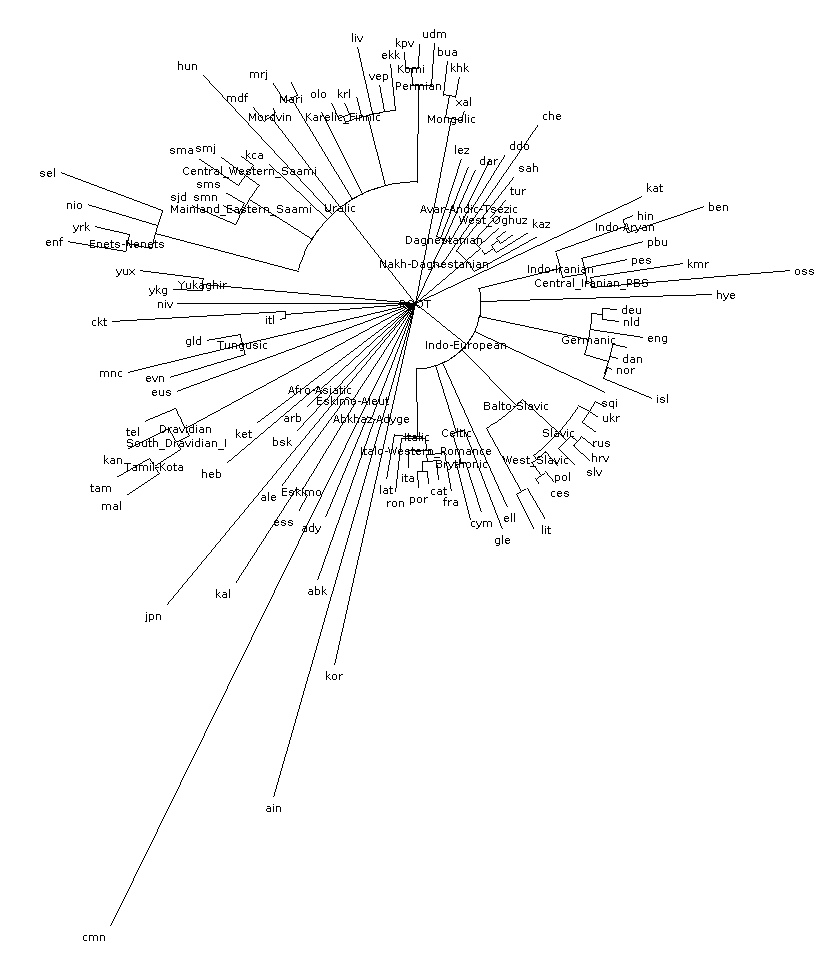
\includegraphics[width=0.9\textwidth]{figures/nelex-tree-with-lengths.png}
 \captionof{figure}{Reduced Glottolog tree with estimated branch lengths}%
 \addtocounter{table}{-1} 
\end{center}

\chapter{Proof of submodularity}
This appendix contains the proof showing that the measure $h(\mathbf{Z})$ for all subsets $\mathbf{Z} = \{Z_1,\dots,Z_m\} \subseteq \mathcal{L}$ of our set of languages $\mathcal{L}$ adheres to the elemental inequalities defining a submodular information measure.\\[0.5cm]
To start with the third condition,
\begin{equation*}
 h(\emptyset) = \sum_{i = 1}^n |\emptyset| = 0.
\end{equation*}\\[0.5cm]
Monotonicity is also trivially true:
\begin{equation*}
  h(\mathbf{Z} \backslash \{L_j\}) = \sum_{i = 1}^n \left(\left|\bigcup_{k=1}^m L_{k,i}(\omega)\right| - \left|L_{j,i}(\omega)\backslash \bigcup_{k=1}^m L_{k,i}(\omega)\right|\right) 
  \leq \sum_{i = 1}^n \left|\bigcup_{k=1}^m L_{k,i}(\omega)\right| = h(\mathbf{Z})
\end{equation*}\\[0.5cm]
Finally, here is the not less elementary proof of the sub-modularity condition:
\begin{multline}
 h(\mathbf{Z}) + h(\mathbf{Z} \cup L_h \cup L_j) 
 = \left|\bigcup_{k=1}^m L_{k,i}(\omega)\right| + \left|\bigcup_{k=1}^m L_{k,i}(\omega) \cup L_{h,i}(\omega) \cup L_{j,i}(\omega)\right|\\
 = 2 \cdot \left|\bigcup_{k=1}^m L_{k,i}(\omega)\right| + \left|L_{h,i}(\omega)\backslash \bigcup_{k=1}^m L_{k,i}(\omega)\right| + \left|L_{j,i}(\omega)\backslash \bigcup_{k=1}^m L_{k,i}(\omega)\right|
       - \left|(L_{h,i}(\omega) \cup L_{j,i}(\omega))\backslash \bigcup_{k=1}^m L_{k,i}(\omega)\right|\\
 \leq 2 \cdot \left|\bigcup_{k=1}^m L_{k,i}(\omega)\right| + \left|L_{h,i}(\omega)\backslash \bigcup_{k=1}^m L_{k,i}(\omega)\right| + \left|L_{j,i}(\omega)\backslash \bigcup_{k=1}^m L_{k,i}(\omega)\right|\\
 = \left|\bigcup_{k=1}^m L_{k,i}(\omega) \cup L_{h,i}(\omega)\right| + \left|\bigcup_{k=1}^m L_{k,i}(\omega) \cup L_{h,j}(\omega)\right|
 = h(\mathbf{Z} \cup L_h) + h(\mathbf{Z} \cup L_j)
\end{multline}

\chapter{Description of supplementary materials}
This appendix describes the contents of the digital supplementary materials distributed together with this thesis. These include the two testsets for cognate detection, the gold standard file for lexical flow on the NorthEuraLex data, the version of NorthEuraLex 0.9 with the inferred cognacy judgments used throughout Chapter 6 and 7, and the Glottolog tree with branch lengths inferred for Chapter 6 (see Appendix B.2). My reference implementations of the algorithms are available in a public repository on Github, and the files for all the simulated scenarios are available for download from my website.

\begin{center}
\small
\begin{longtable}{ll}
\hline \hline
 \textbf{File} & \textbf{Description}\\
\hline
\endfirsthead
\hline \hline
 \textbf{File} & \textbf{Description}\\
\hline
\endhead
\hline\\
\endfoot
\hline
\endlastfoot

 \texttt{cognacy-eval-pairs.tsv} 
  & The cognate detection testset derived from IELex.\\
  & One pair of words for the same concept per line.\\
  & First column is the NorthEuraLex concept ID,\\
  & followed by two blocks of four columns,\\
  & each defining a term by the ISO 639-3 code,\\
  & the orthographic form, the simplified\\
  & IPA representation, and a form ID. The last\\
  & column encodes cognacy according to IELex:\\
  & \texttt{T} for cognate pairs, \texttt{F} for non-cognate pairs.\\
 \hline
  \texttt{wold-nelex-intersect.tsv} 
  & Lists all instances of borrowings from WOLD\\
  & where both loanword and its source are in NELex.\\
  & Column 3 contains the loan in notation \textit{iso}:\textit{orth},\\
  & Column 4 the source word in the same format.\\
  & Column 2 is \texttt{wold} for borrowing events which\\
  & appear exactly identically in both databases,\\
  & and \texttt{woldx} if some adaptation was necessary.\\
  & Column 1 is always \texttt{1} (high confidence only).\\
 \hline
  \texttt{nelex-gold-standard-contact.txt} 
  & PLFI gold standard, one contact per line\\
  & in machine-readable format of form \texttt{A rel B}.\\
  & Language names from ISO 639-3 or Glottolog.\\
  & The symbol \texttt{-->} is for cross-family contacts,\\
  & \texttt{o->} for directional contacts within families.\\
 \hline
  \texttt{inferred-cognates.tsv} 
  & Inferred cognate sets over NorthEuraLex 0.9 for a\\
  & UPGMA threshold of 0.45, in a 5-column format.\\
  & Concept ID in Column 1, ISO 639-3 in Column 2,\\
  & orthography and IPA string in Columns 3 and 4,\\
  & Column 5 a numeric set ID (separate per concept).\\
 \hline
  \texttt{nelex-tree-with-lengths.nwk} 
  & Glottolog tree reduced to NorthEuraLex languages,\\
  & with inferred branch lengths, in Newick format.\\
\end{longtable}
\end{center}

  
% % copy the lines above and adapt as necessary

%%%%%%%%%%%%%%%%%%%%%%%%%%%%%%%%%%%%%%%%%%%%%%%%%%%% 
%%%             Backmatter                       %%% 
%%%%%%%%%%%%%%%%%%%%%%%%%%%%%%%%%%%%%%%%%%%%%%%%%%%%

%\is{some term| see {some other term}}
%\il{some language| see {some other language}}
%\issa{some term with pages}{some other term also of interest}
%\ilsa{some language with pages}{some other lect also of interest}
 
\iasa{Aikio, Antex}{Ánte, Luobbal Sámmol Sámmol}
\iasa{Ántex, Luobbal Sámmol Sámmol}{Aikio, Ante}
 
 
% There is normally no need to change the backmatter section
\sloppy
\backmatter
\phantomsection%this allows hyperlink in ToC to work
{\sloppy\printbibliography[heading=\lsReferencesTitle]}
\cleardoublepage

\phantomsection 
\addcontentsline{toc}{chapter}{\lsIndexTitle} 
\addcontentsline{toc}{section}{\lsNameIndexTitle}
\ohead{\lsNameIndexTitle} 
\printindex 
\cleardoublepage
  
\phantomsection 
\addcontentsline{toc}{section}{\lsLanguageIndexTitle}
\ohead{\lsLanguageIndexTitle} 
\printindex[lan] 
\cleardoublepage
  
\phantomsection 
\addcontentsline{toc}{section}{\lsSubjectIndexTitle}
\ohead{\lsSubjectIndexTitle} 
\printindex[sbj]
\ohead{} 
 
\end{document} 

% you can create your book by running
% xelatex main.tex 
